% Options for packages loaded elsewhere
% Options for packages loaded elsewhere
\PassOptionsToPackage{unicode}{hyperref}
\PassOptionsToPackage{hyphens}{url}
\PassOptionsToPackage{dvipsnames,svgnames,x11names}{xcolor}
%
\documentclass[
  hebrew,
  letterpaper,
  DIV=11,
  numbers=noendperiod]{scrreprt}
\usepackage{xcolor}
\usepackage{amsmath,amssymb}
\setcounter{secnumdepth}{5}
\usepackage{iftex}
\ifPDFTeX
  \usepackage[T1]{fontenc}
  \usepackage[utf8]{inputenc}
  \usepackage{textcomp} % provide euro and other symbols
\else % if luatex or xetex
  \usepackage{unicode-math} % this also loads fontspec
  \defaultfontfeatures{Scale=MatchLowercase}
  \defaultfontfeatures[\rmfamily]{Ligatures=TeX,Scale=1}
\fi
\usepackage{lmodern}
\ifPDFTeX\else
  % xetex/luatex font selection
  \setmainfont[]{Arial}
  \setsansfont[]{Arial}
\fi
% Use upquote if available, for straight quotes in verbatim environments
\IfFileExists{upquote.sty}{\usepackage{upquote}}{}
\IfFileExists{microtype.sty}{% use microtype if available
  \usepackage[]{microtype}
  \UseMicrotypeSet[protrusion]{basicmath} % disable protrusion for tt fonts
}{}
\makeatletter
\@ifundefined{KOMAClassName}{% if non-KOMA class
  \IfFileExists{parskip.sty}{%
    \usepackage{parskip}
  }{% else
    \setlength{\parindent}{0pt}
    \setlength{\parskip}{6pt plus 2pt minus 1pt}}
}{% if KOMA class
  \KOMAoptions{parskip=half}}
\makeatother
% Make \paragraph and \subparagraph free-standing
\makeatletter
\ifx\paragraph\undefined\else
  \let\oldparagraph\paragraph
  \renewcommand{\paragraph}{
    \@ifstar
      \xxxParagraphStar
      \xxxParagraphNoStar
  }
  \newcommand{\xxxParagraphStar}[1]{\oldparagraph*{#1}\mbox{}}
  \newcommand{\xxxParagraphNoStar}[1]{\oldparagraph{#1}\mbox{}}
\fi
\ifx\subparagraph\undefined\else
  \let\oldsubparagraph\subparagraph
  \renewcommand{\subparagraph}{
    \@ifstar
      \xxxSubParagraphStar
      \xxxSubParagraphNoStar
  }
  \newcommand{\xxxSubParagraphStar}[1]{\oldsubparagraph*{#1}\mbox{}}
  \newcommand{\xxxSubParagraphNoStar}[1]{\oldsubparagraph{#1}\mbox{}}
\fi
\makeatother


\usepackage{longtable,booktabs,array}
\usepackage{calc} % for calculating minipage widths
% Correct order of tables after \paragraph or \subparagraph
\usepackage{etoolbox}
\makeatletter
\patchcmd\longtable{\par}{\if@noskipsec\mbox{}\fi\par}{}{}
\makeatother
% Allow footnotes in longtable head/foot
\IfFileExists{footnotehyper.sty}{\usepackage{footnotehyper}}{\usepackage{footnote}}
\makesavenoteenv{longtable}
\usepackage{graphicx}
\makeatletter
\newsavebox\pandoc@box
\newcommand*\pandocbounded[1]{% scales image to fit in text height/width
  \sbox\pandoc@box{#1}%
  \Gscale@div\@tempa{\textheight}{\dimexpr\ht\pandoc@box+\dp\pandoc@box\relax}%
  \Gscale@div\@tempb{\linewidth}{\wd\pandoc@box}%
  \ifdim\@tempb\p@<\@tempa\p@\let\@tempa\@tempb\fi% select the smaller of both
  \ifdim\@tempa\p@<\p@\scalebox{\@tempa}{\usebox\pandoc@box}%
  \else\usebox{\pandoc@box}%
  \fi%
}
% Set default figure placement to htbp
\def\fps@figure{htbp}
\makeatother

\ifLuaTeX
  \usepackage{luacolor}
  \usepackage[soul]{lua-ul}
\else
  \usepackage{soul}
\fi


\ifLuaTeX
\usepackage[bidi=basic,provide=*]{babel}
\else
\usepackage[bidi=default,provide=*]{babel}
\fi
\ifPDFTeX
\else
\babelfont{rm}[]{Arial}
\fi
% get rid of language-specific shorthands (see #6817):
\let\LanguageShortHands\languageshorthands
\def\languageshorthands#1{}


\setlength{\emergencystretch}{3em} % prevent overfull lines

\providecommand{\tightlist}{%
  \setlength{\itemsep}{0pt}\setlength{\parskip}{0pt}}

\ifPDFTeX
  \TeXXeTstate=1
  \newcommand{\RL}[1]{\beginR #1\endR}
  \newcommand{\LR}[1]{\beginL #1\endL}
  \newenvironment{RTL}{\beginR}{\endR}
  \newenvironment{LTR}{\beginL}{\endL}
\fi


 


\usepackage{bidi}

% Force RTL for the whole document
\AtBeginDocument{\setRTL}

% Make underline safe: override soul \ul AFTER packages load
\AtBeginDocument{\renewcommand{\ul}[1]{\underline{#1}}}
\KOMAoption{captions}{tableheading}
\makeatletter
\@ifpackageloaded{tcolorbox}{}{\usepackage[skins,breakable]{tcolorbox}}
\@ifpackageloaded{fontawesome5}{}{\usepackage{fontawesome5}}
\definecolor{quarto-callout-color}{HTML}{909090}
\definecolor{quarto-callout-note-color}{HTML}{0758E5}
\definecolor{quarto-callout-important-color}{HTML}{CC1914}
\definecolor{quarto-callout-warning-color}{HTML}{EB9113}
\definecolor{quarto-callout-tip-color}{HTML}{00A047}
\definecolor{quarto-callout-caution-color}{HTML}{FC5300}
\definecolor{quarto-callout-color-frame}{HTML}{acacac}
\definecolor{quarto-callout-note-color-frame}{HTML}{4582ec}
\definecolor{quarto-callout-important-color-frame}{HTML}{d9534f}
\definecolor{quarto-callout-warning-color-frame}{HTML}{f0ad4e}
\definecolor{quarto-callout-tip-color-frame}{HTML}{02b875}
\definecolor{quarto-callout-caution-color-frame}{HTML}{fd7e14}
\makeatother
\makeatletter
\@ifpackageloaded{bookmark}{}{\usepackage{bookmark}}
\makeatother
\makeatletter
\@ifpackageloaded{caption}{}{\usepackage{caption}}
\AtBeginDocument{%
\ifdefined\contentsname
  \renewcommand*\contentsname{תוכן עניינים}
\else
  \newcommand\contentsname{תוכן עניינים}
\fi
\ifdefined\listfigurename
  \renewcommand*\listfigurename{רשימת תרשימים}
\else
  \newcommand\listfigurename{רשימת תרשימים}
\fi
\ifdefined\listtablename
  \renewcommand*\listtablename{רשימת טבלאות}
\else
  \newcommand\listtablename{רשימת טבלאות}
\fi
\ifdefined\figurename
  \renewcommand*\figurename{תרשים}
\else
  \newcommand\figurename{תרשים}
\fi
\ifdefined\tablename
  \renewcommand*\tablename{טבלה}
\else
  \newcommand\tablename{טבלה}
\fi
}
\@ifpackageloaded{float}{}{\usepackage{float}}
\floatstyle{ruled}
\@ifundefined{c@chapter}{\newfloat{codelisting}{h}{lop}}{\newfloat{codelisting}{h}{lop}[chapter]}
\floatname{codelisting}{רישום}
\newcommand*\listoflistings{\listof{codelisting}{רשימת רישומים}}
\makeatother
\makeatletter
\makeatother
\makeatletter
\@ifpackageloaded{caption}{}{\usepackage{caption}}
\@ifpackageloaded{subcaption}{}{\usepackage{subcaption}}
\makeatother
\usepackage{bookmark}
\IfFileExists{xurl.sty}{\usepackage{xurl}}{} % add URL line breaks if available
\urlstyle{same}
\hypersetup{
  pdftitle={מבוא להנדסת תהליכים},
  pdfauthor={ענבל צרפתי-ברעד},
  pdflang={he},
  colorlinks=true,
  linkcolor={blue},
  filecolor={Maroon},
  citecolor={Blue},
  urlcolor={Blue},
  pdfcreator={LaTeX via pandoc}}


\title{מבוא להנדסת תהליכים}
\author{ענבל צרפתי-ברעד}
\date{}
\begin{document}
\maketitle

\renewcommand*\contentsname{תוכן עניינים}
{
\hypersetup{linkcolor=}
\setcounter{tocdepth}{2}
\tableofcontents
}

\bookmarksetup{startatroot}

\chapter*{מבוא להנדסת
תהליכים}\label{ux5deux5d1ux5d5ux5d0-ux5dcux5d4ux5e0ux5d3ux5e1ux5ea-ux5eaux5d4ux5dcux5d9ux5dbux5d9ux5dd}
\addcontentsline{toc}{chapter}{מבוא להנדסת תהליכים}

\markboth{מבוא להנדסת תהליכים}{מבוא להנדסת תהליכים}

\section*{ד''ר ענבל
צרפתי-ברעד}\label{ux5d3ux5e8-ux5e2ux5e0ux5d1ux5dc-ux5e6ux5e8ux5e4ux5eaux5d9-ux5d1ux5e8ux5e2ux5d3}
\addcontentsline{toc}{section}{ד''ר ענבל צרפתי-ברעד}

\markright{ד''ר ענבל צרפתי-ברעד}

מיועד לסטודנטים וסטודנטיות בתחילת דרכם בתחום הנדסת תהליכים

תודות

ד״ר רחל ליכטנשטיין, המחלקה להנדסת ביוטכנולוגיה על שם אברם וסטלה
גולדשטיין־גורן פרופ׳ רונית ביטון, המחלקה להנדסה כימית היחידה לקידום
איכות ההוראה והלמידה אוניברסיטת בן־גוריון בנגב

\bookmarksetup{startatroot}

\chapter*{\texorpdfstring{{הקדמה}}{הקדמה}}\label{ux5d4ux5e7ux5d3ux5deux5d4}
\addcontentsline{toc}{chapter}{{הקדמה}}

\markboth{{הקדמה}}{{הקדמה}}

{בשנת 2020 התפרצה מגפת הקורונה והציבה בפני האנושות אתגר חסר תקדים: בתוך
פרק זמן קצר מאוד נדרש היה לפתח, לייצר ולחלק מיליארדי מנות חיסון ברחבי
העולם. מצד אחד, ההישג המדעי היה דרמטי -- בתוך פחות משנה פותחו חיסונים
חדשניים, חלקם בטכנולוגיות שלא נוסו קודם בקנה מידה עולמי. מצד שני, האתגר
לא הסתיים ברמת המחקר במעבדה: השלב הקריטי בקביעת קצב ההתחסנות של
האוכלוסיות היה אתגר של \textbf{העברה מפתרון ניסויי לייצור תעשייתי בקנה
מידה עצום}}.

{חברות התרופות נאלצו להקים קווי ייצור חדשים או להרחיב מתקנים קיימים
במהירות מסחררת. תהליכים שנמשכים בדרך כלל שנים ארוכות -- בניית מפעלים,
התאמת ציוד, והבטחת איכות קפדנית -- התרחשו תוך חודשים ספורים. כל שלב דרש
תיאום הדוק בין מהנדסי ומהנדסות תהליכים, מהנדסי ומהנדסות ביוטכנולוגיה,
אנשי ונשות רגולציה וגם כלכלנים וכלכלניות. מעבר לכך, יצרנים התמודדו עם
מחסור עולמי בציוד, בחומרי גלם ובכוח אדם מיומן}. {הרגולטורים נדרשו אף הם
להתאים את עצמם: במקום מסלול אישור ארוך ומדורג, נבנו מנגנוני "אישור
חירום" שעדיין שמרו על רמות בטיחות גבוהות אך איפשרו הפעלה מהירה של
מתקנים. ועדיין, לא כל הבעיות נפתרו בבת אחת. קצב ההתחסנות הושפע לא רק
מפיתוח החיסונים והוכחת יעילותם, אלא גם מיכולת הייצור, מהאישורים
הלוגיסטיים, ומהאתגרים של הפצה בקירור עמוק לכל נקודה על פני הגלובוס}.

{בחורף 2020--2021, עם תחילת מתן החיסונים נגד קורונה, הכמות שהגיעה לכל
מדינה הייתה מוגבלת מאוד. החיסונים הראשונים נשמרו בקפידה לקבוצות בסיכון
גבוה: צוותי רפואה, קשישים, וחולים כרוניים. רוב הציבור נאלץ להמתין
בסבלנות, כשברקע התפרסמו שוב ושוב תמונות של תורים ארוכים למנות חיסון
עודפות, שהיו עומדות לפוג תוך שעות ספורות. עבור רבים זו הייתה החוויה
הראשונה של "מחסור רפואי גלובלי": להבין שיש תרופה או חיסון שיכול להציל
חיים -- אבל היכולת לייצר ולהפיץ אותו מוגבלת מאוד}. {המצב הזה השתנה
בהדרגה. בתוך חודשים ספורים, ייצור החיסונים הפך לפרויקט תעשייתי עצום בקנה
מידה עולמי. אם בתחילת הדרך נספרו כל קרטון וכל בקבוקון, הרי שבסוף 2021
כבר יוצרו מעל 10 מיליארד מנות חיסון -- קצב שלא נראה כמותו בהיסטוריה של
התעשייה התרופתית. המעבר ממחסור חריף לשפע יחסי התרחש בזכות שילוב של
טכנולוגיות חדשות, הרחבת קווי ייצור, רגולציה מואצת ושיתוף פעולה
בינלאומי}.

{הסיפור הזה מדגיש היטב את תפקידה של הנדסת תהליכים: היא זו שמאפשרת להפוך
הישג מדעי נקודתי להישג מעשי בקנה מידה עולמי -- במהירות, באמינות, ובעלות
סבירה. ללא ההתרחבות הדרמטית של יכולות הייצור, החיסונים היו נשארים
במעבדות ובמרכזי מחקר, רחוקים מן האנשים שהיו זקוקים להם ביותר}. {מהנדסי
ומהנדסות תהליכים הם מי שמתרגמים ידע מדעי לתשתית תעשייתית ברת-קיימא, והם
ממלאים תפקיד קריטי בכל תחום שבו נדרשת הנדסה בקנה מידה גדול -- מתעשיית
המזון והתרופות ועד לאנרגיה ולכימיה מתקדמת}.

{במובן זה, מגפת הקורונה שימשה "שיעור חי" לעולם כולו: היא המחישה כיצד
אתגרים גלובליים תלויים לא רק במדע, אלא גם בהנדסה שמאפשרת להפוך רעיון
למציאות}. {הנדסת תהליכים היא הסיפור הזה -- איך מולקולה שנבדקה במעבדה
הופכת לחיסון שמציל חיים. איך חדשנות הופכת לאוכל על המדף, לאנרגיה נקייה,
או לשבב מחשב שמניע את הטלפון שלכם}. {הספר שלפניכם לא בא רק ללמד חוקים,
משוואות או דיאגרמות. הוא בא לספר את הסיפור של תחום שמחבר בין מדע לבין
חיים אמיתיים. תחום שנמצא בכל מקום -- גם אם לפעמים לא שמים לב.}

\bookmarksetup{startatroot}

\chapter{\texorpdfstring{{מה עושים מהנדסי ומהנדסות
תהליך?}}{מה עושים מהנדסי ומהנדסות תהליך?}}\label{ux5deux5d4-ux5e2ux5d5ux5e9ux5d9ux5dd-ux5deux5d4ux5e0ux5d3ux5e1ux5d9-ux5d5ux5deux5d4ux5e0ux5d3ux5e1ux5d5ux5ea-ux5eaux5d4ux5dcux5d9ux5da}

\section{\texorpdfstring{{מהי הנדסת
תהליך}?}{מהי הנדסת תהליך?}}\label{ux5deux5d4ux5d9-ux5d4ux5e0ux5d3ux5e1ux5ea-ux5eaux5d4ux5dcux5d9ux5da}

{הנדסת תהליך היא תחום הנדסי-מדעי רחב, העוסק בהמרת חומרי גלם למוצרים בעלי
ערך כלכלי או חברתי, באמצעות תהליכים מתוכננים ומבוקרים. בניגוד למדע
"טהור", שמבקש להבין תופעות טבע, מטרתה של הנדסת תהליך היא \textbf{לרתום
את הידע המדעי לצורך יישום מעשי}}. {מהנדסי תהליך שואלים לא רק \emph{מהי}
תגובה כימית או ביולוגית, אלא גם \emph{כיצד ניתן לתרגם אותה לייצור
תעשייתי} - יציב, בטוח, כלכלי ובר-קיימא}.

{התחום משלב ידע ממדעים בסיסיים -- כימיה, ביולוגיה, פיזיקה ומתמטיקה --
יחד עם כלים הנדסיים ותפיסה מערכתית. השאלה המרכזית היא תמיד מערכתית: איך
הופכים תהליך מקומי או תופעה מדעית לתהליך כולל, שבו חומרי גלם מוזרמים,
מומרצים, עוברים שינוי, מופרדים, ומניבים מוצר איכותי}?

{כיוון שהנדסת תהליך עוסקת \emph{בדרכים} ולא רק \emph{בתוצרים}}, {היא
מיושמת במגוון עצום של תחומים}.

{בתעשייה הכימית, לדוגמה, הנדסת תהליך מאפשרת ייצור של פולימרים, דשנים
ומתכות בקנה מידה עולמי. בתחום הביוטכנולוגיה היא מאפשרת הפקה של חלבונים,
חיסונים ותרופות, לעיתים באמצעות תאים חיים או אנזימים, תוך שמירה על תנאים
אופטימליים לריאקציה הביולוגית}. {מעבר לכך, הנדסת תהליך נוגעת גם באנרגיה
-- למשל בפיתוח דלק ביולוגי מאצות}; {בסביבה -- באמצעות טיפול בשפכים
תעשייתיים בעזרת ביוריאקטורים}; {ובמזון -- למשל בייצור יוגורט תעשייתי},
{שבו שליטה בתנאי התסיסה היא קריטית}.

{בכל התחומים הללו חוזרת אותה לוגיקה הנדסית\ul{: פירוק הבעיה ליחידות
פעולה (חימום, קירור, ערבוב, זרימה, ספיגה, הפרדה) ושילובן לתהליך
כולל}}\ul{.}

\subsection{\texorpdfstring{{מה מבדיל בין ביוטכנולוגים למהנדסי
ביוטכנולוגיה}?}{מה מבדיל בין ביוטכנולוגים למהנדסי ביוטכנולוגיה?}}\label{ux5deux5d4-ux5deux5d1ux5d3ux5d9ux5dc-ux5d1ux5d9ux5df-ux5d1ux5d9ux5d5ux5d8ux5dbux5e0ux5d5ux5dcux5d5ux5d2ux5d9ux5dd-ux5dcux5deux5d4ux5e0ux5d3ux5e1ux5d9-ux5d1ux5d9ux5d5ux5d8ux5dbux5e0ux5d5ux5dcux5d5ux5d2ux5d9ux5d4}

{ביוטכנולוגים וביוטכנולוגיות מתמקדים בחקר מערכות ביולוגיות בקנה מידה
קטן: הם מפתחים שיטות מעבדתיות חדשות, מאפיינים תאים וחלבונים, ומגלים
דרכים לנצל מנגנונים ביולוגיים ליצירת חומרים ותרופות. עבודתם עוסקת בשאלה
\emph{האם תהליך ביולוגי מסוים מתרחש וכיצד ניתן להשתמש בו
לרווחתנו}}\emph{?}

{מהנדסי ומהנדסות ביוטכנולוגיה, לעומת זאת, לוקחים את הממצאים הללו
ומתרגמים אותם למערכות בקנה מידה תעשייתי. הם מתמודדים עם האתגר של הפיכת
תהליכים עדינים ורגישים, כמו גידול תאים, ייצור חלבונים רקומביננטיים או
תסיסה מיקרוביאלית, למערכות יציבות, מבוקרות ורווחיות}.\\
{המשימה שלהם אינה רק להבין את התהליך, אלא להפוך אותו ליישים במפעל
ביוטכנולוגי}.

{אתגרים מרכזיים בעבודת מהנדס ביוטכנולוגיה כוללים}:

\begin{itemize}
\item
  {\textbf{אספקת חומרי גלם ביולוגיים}} -- {תאים, מצעי גידול, אנזימים}.
\item
  {\textbf{תכנון ביוריאקטורים}} -- {שליטה בלחץ, טמפרטורה}, pH, {רמות
  חמצן והזנה לקבלת מערכת הומוגנית}
\item
  {\textbf{הפרדת תוצרים}} -- {טיהור חלבונים, סינון תאים, הפרדת תרכובות
  מורכבות}.
\item
  {\textbf{בטיחות ביולוגית}} -- {מניעת זיהומים, עבודה בתנאים סטריליים,
  מניעת שחרור מיקרואורגניזמים}.
\end{itemize}

{במילים אחרות: הביוטכנולוג שואל} \emph{``{האם התא מייצר את
החלבון?"}\emph{{מהנדס הביוטכנולוגיה שואל} }''{איך אני מייצר מיליון מנות
תרופה בצורה יציבה, בטוחה ורווחית}?{}``}

\subsection{\texorpdfstring{{היבטים משלימים: כלכלה, רגולציה
וסביבה}}{היבטים משלימים: כלכלה, רגולציה וסביבה}}\label{ux5d4ux5d9ux5d1ux5d8ux5d9ux5dd-ux5deux5e9ux5dcux5d9ux5deux5d9ux5dd-ux5dbux5dcux5dbux5dcux5d4-ux5e8ux5d2ux5d5ux5dcux5e6ux5d9ux5d4-ux5d5ux5e1ux5d1ux5d9ux5d1ux5d4}

{כדי שתהליך ביוטכנולוגי יהפוך ממחקר מעבדתי לייצור תעשייתי, יש לשקלל
שלושה ממדים נוספים מעבר לצד הטכני-מדעי}:

\begin{itemize}
\item
  {\textbf{כלכלה}} -- {ייצור בקנה מידה גדול דורש חישוב עלויות של מצעי
  גידול, מערכות סטריליזציה, אנרגיה ותפעול. אם שלב הטיהור של חלבון יקר
  מדי -- המוצר לא יוכל לצאת לשוק}.
\item
  {\textbf{רגולציה}} -- {מוצרי ביוטכנולוגיה (כמו חיסונים או תרופות
  מבוססות תאים) כפופים לסטנדרטים מחמירים של רשויות בריאות. נדרש תיעוד
  מלא, בקרת איכות רציפה ותהליכי ייצור נקיים} (GMP).
\item
  {\textbf{סביבה}} -- {תהליכים ביוטכנולוגיים יוצרים פסולת ביולוגית
  ושפכים תעשייתיים. יש צורך בשיטות טיפול, ניטרול והשבה כדי למזער נזקים
  סביבתיים ולשמור על קיימות}.
\end{itemize}

{האיזון בין שלושת ההיבטים הללו -- כלכלה, רגולציה וסביבה -- לצד הידע
המדעי וההנדסי, הוא שמאפשר למהנדסי ביוטכנולוגיה להפוך תגלית ביולוגית
למערכת ייצור תעשייתית שמספקת ערך אמיתי לחברה}.

\section{\texorpdfstring{{איך נראית עבודת מהנדס ומהנדסת
התהליך}?}{איך נראית עבודת מהנדס ומהנדסת התהליך?}}\label{ux5d0ux5d9ux5da-ux5e0ux5e8ux5d0ux5d9ux5ea-ux5e2ux5d1ux5d5ux5d3ux5ea-ux5deux5d4ux5e0ux5d3ux5e1-ux5d5ux5deux5d4ux5e0ux5d3ux5e1ux5ea-ux5d4ux5eaux5d4ux5dcux5d9ux5da}

{עבודתם של מהנדסי ומהנדסות התהליך מורכבת ממספר שלבים עיקריים. שלבים אלו
אינם תמיד לינאריים -- לעיתים חוזרים אחורה, בוחנים חלופות חדשות או משנים
פרמטרים בהתאם לנתונים שמתקבלים}.

\textbf{{שלבים מרכזיים בהנדסת תהליך:}}

\begin{longtable}[]{@{}
  >{\raggedleft\arraybackslash}p{(\linewidth - 4\tabcolsep) * \real{0.3333}}
  >{\raggedleft\arraybackslash}p{(\linewidth - 4\tabcolsep) * \real{0.3333}}
  >{\raggedleft\arraybackslash}p{(\linewidth - 4\tabcolsep) * \real{0.3333}}@{}}
\toprule\noalign{}
\begin{minipage}[b]{\linewidth}\raggedleft
\textbf{שלב}
\end{minipage} & \begin{minipage}[b]{\linewidth}\raggedleft
\textbf{תיאור}
\end{minipage} & \begin{minipage}[b]{\linewidth}\raggedleft
\textbf{דוגמה}
\end{minipage} \\
\midrule\noalign{}
\endhead
\bottomrule\noalign{}
\endlastfoot
\textbf{אפיון הבעיה והגדרת מטרות} & זיהוי הצורך: ייצור חדש/שיפור/הפחתת
עלויות.קביעת יעדים כמותיים ואיכותיים (כמות ייצור, רמת טוהר, דרישות
רגולציה). & חברת ביוטכנולוגיה שרוצה לייצר חיסון מגדירה מראש כמה מנות
לשנה, טווח טמפרטורות לשימור, ואילו תקנים נדרשים. \\
\textbf{פיתוח ראשוני של התהליך} & בחירת מסלול תגובה או שיטה ביוטכנולוגית
(כימית/אנזימטית/ביולוגית).בחינת תנאים פיזיקליים (טמפרטורה, לחץ, pH,
ריכוזים). & בייצור בירה: תסיסת סוכרים לאלכוהול; בחירת זן שמרים, טמפרטורה
וזמן תסיסה. \\
\textbf{תכנון יחידות פעולה} & קביעת סוג הריאקטור (רציף/אצווה; עם/בלי
ערבוב).תכנון שלבי הפרדה (סינון, זיקוק, מיצוי).תכנון מערכות תומכות:
חימום, קירור, ערבוב, אוורור. & אתנול מדלק ביולוגי: ריאקטור לתסיסה +
זיקוק להפרדת אתנול־מים. \\
\textbf{שיקולי כלכלה ובטיחות} & בחינת עלויות חומרי גלם, אנרגיה
ותפעול.עמידה בתקני בטיחות ותכנון למניעת כשלים (לחץ יתר, טמפרטורה חריגה).
& תהליך הבר--בוש (אמוניה): תכנון מערכות בטיחות ללחצים גבוהים ויציבות
הכלים. \\
\textbf{בקרה ואופטימיזציה} & הטמעת מערכות בקרה בזמן אמת.ניתוח נתוני
תהליך ושיפורים מתמשכים. & ייצור אינסולין רקומביננטי: בקרה רציפה של pH
והריכוזים למקסום תפוקה והפחתת הפסדים. \\
\end{longtable}

\section{\texorpdfstring{{פתרון בעיות בהנדסת
תהליך}}{פתרון בעיות בהנדסת תהליך}}\label{ux5e4ux5eaux5e8ux5d5ux5df-ux5d1ux5e2ux5d9ux5d5ux5ea-ux5d1ux5d4ux5e0ux5d3ux5e1ux5ea-ux5eaux5d4ux5dcux5d9ux5da}

{פתרון בעיות הוא ליבת ההנדסה, ובמיוחד בהנדסת תהליך. אך חשוב להדגיש:
בניגוד לבעיות מתמטיות "טהורות", בעיות הנדסיות עוסקות במציאות, והמציאות
אינה ניתנת לתיאור מושלם}.

\subsection{\texorpdfstring{{מודלים כקירוב
למציאות}}{מודלים כקירוב למציאות}}\label{ux5deux5d5ux5d3ux5dcux5d9ux5dd-ux5dbux5e7ux5d9ux5e8ux5d5ux5d1-ux5dcux5deux5e6ux5d9ux5d0ux5d5ux5ea}

{בהנדסת תהליך אנו עושים שימוש במודלים מתמטיים -- משוואות מאזני חומר,
אנרגיה ותנע, משוואות קינטיות, מודלים אמפיריים ועוד -- כדי לתאר תהליכים
מורכבים. המודל מאפשר חישוב, חיזוי ואופטימיזציה}.\\
{אולם, המודלים הם תמיד \textbf{קירוב}}:

\begin{itemize}
\item
  {הם מתבססים על הנחות (לדוגמה: זרימה למינרית, מצב יציב, תגובה
  חד-שלבית)}.
\item
  {הם מפשטים מצבים מורכבים (למשל, מניחים שהתערובת אידיאלית או שהתנאים
  אחידים בכל המערכת)}.
\item
  {הם מתעלמים לעיתים מגורמים "קטנים" שבמציאות עשויים להיות משמעותיים
  (למשל, זיהום זעיר שמוביל לשינוי התוצאה)}.
\end{itemize}

{למרות זאת, מודלים טובים משמשים לחיסכון בזמן ומשאבים. תיאור מתמטי מלא של
מערכת פיזיקלית או ביולוגית יהיה בדרך כלל כה מורכב, עד שלא ניתן לפתור
אותו באופן אנליטי. גם אם נכתוב את המודל "המדויק ביותר", בסופו של דבר
ניאלץ להשתמש בקירובים נומריים שמכניסים שגיאות משלהם. לכן, לעיתים דווקא
מודל פשוט יותר מספק תובנות שימושיות יותר -- מפני שקל יותר לחשב אותו
ולבצע עליו ניתוחים}.

{במילים אחרות, המודל אינו "האמת", אלא כלי עבודה שמאפשר לנו להתקדם. כפי
שצוטט הסטטיסטיקאי ג'ורג' אי. פ. בוקס} (George E. P. Box){:}

\emph{"All models are wrong, but some are useful."}

{המהנדס חייב לדעת \textbf{להשתמש במודל בלי ליפול לאשליה שהוא המציאות
עצמה-} לדעת מתי המודל מספיק שימושי, ואילו שגיאות הוא מכניס לתמונה}. {לכן
חלק מהבעיה הוא גם לשאול: \emph{עד כמה הפתרון רלוונטי? מהי רמת הדיוק
הדרושה}}\emph{?}

\subsection{\texorpdfstring{{אסטרטגיות לפתרון
בעיות}}{אסטרטגיות לפתרון בעיות}}\label{ux5d0ux5e1ux5d8ux5e8ux5d8ux5d2ux5d9ux5d5ux5ea-ux5dcux5e4ux5eaux5e8ux5d5ux5df-ux5d1ux5e2ux5d9ux5d5ux5ea}

{פתרון בעיות בהנדסה איננו חד-כיווני. קיימות מספר גישות שיכולות לסייע}:

\begin{enumerate}
\def\labelenumi{\arabic{enumi}.}
\item
  \textbf{{גישה מההתחלה לסוף} (forward problem solving)}\\
  {מתחילים מהנתונים הידועים ומתקדמים שלב אחר שלב באמצעות המודלים עד
  לתוצאה המבוקשת}. {זה נוח כאשר יש שיטה מסודרת או שיש לנו את כל הנתונים
  מלאים. אבל} {אם יש נתון חסר או טעות בהתחלה -- אנחנו עלולים להתקע
  במקום, או להתפזר לחישובים שאינם רלוונטיים.}
\item
  \textbf{{גישה מהסוף להתחלה} {}(backward problem solving)}\\
  {מתחילים מהתוצאה הרצויה (מה אנחנו רוצים לדעת או לחשב) וחושבים לאחור:
  אילו משתנים דרושים כדי להגיע לשם? אילו משוואות עלינו להפעיל}? {}
\item
  \textbf{{גישה מהאמצע} (identifying the bottleneck)}\\
  {לעיתים הבעיה נתקעת סביב שלב מסוים -- למשל חוסר נתון קריטי, או משוואה
  שאיננו יודעים כיצד ליישם. במקרה כזה כדאי להתחיל דווקא מהנקודה הבעייתית
  ביותר, לפרק אותה, ולהמשיך ממנה קדימה ואחורה}.
\item
  \textbf{{גישה אינטגרטיבית} {}(mixed strategies)}\\
  {לרוב הפתרון אינו מתבצע בגישה אחת בלבד אלא בשילוב: מתחילים מהנתונים
  הידועים, מזהים את החסר, חושבים לאחור מהתוצאה, ולעיתים עוצרים באמצע כדי
  להתמודד עם מכשול נקודתי}.
\end{enumerate}

{כאשר נתקלים בשאלה ארוכה או מורכבת, לא ניגשים מיד לחישובים. פתרון בעיות
בהנדסה דורש סדר מחשבתי, ארגון מידע והסקת מסקנות מבוססות. התרשים הבא מציג
תהליך שיטתי --- מעין "אלגוריתם הנדסי" --- המסייע לגשת לכל שאלה בצורה
מסודרת: לקרוא, לנתח, לבחור כלים, להציב נתונים ולבדוק את סבירות התוצאה}.

\begin{tcolorbox}[enhanced jigsaw, colback=white, arc=.35mm, coltitle=black, breakable, toptitle=1mm, leftrule=.75mm, colbacktitle=quarto-callout-tip-color!10!white, opacitybacktitle=0.6, bottomtitle=1mm, titlerule=0mm, opacityback=0, colframe=quarto-callout-tip-color-frame, title=\textcolor{quarto-callout-tip-color}{\faLightbulb}\hspace{0.5em}{עצה}, rightrule=.15mm, bottomrule=.15mm, toprule=.15mm, left=2mm]

\textbf{{\ul{שלב א: ניתוח והגדרת הבעיה}}}

\begin{enumerate}
\def\labelenumi{\arabic{enumi}.}
\item
  {קריאה מהירה לסריקה כללית, ואז קריאה מדויקת של השאלה}.
\item
  {ניסוח היעד במילים שלך: מה בדיוק נדרש לחשב/להראות}.
\item
  {ציור דיאגרמה של המערכת; סימון נתונים ידועים (עם יחידות) ובלתי־ידועים
  (אותיות)}.
\item
  {זיהוי רמזים מילוליים (למשל ``גדול/קטן מאוד'', ``בקירוב'', ``בהשוואה
  ל--'') ושיוכם לתובנות הנדסיות}.
\end{enumerate}

\textbf{{\ul{שלב ב: תכנון הפתרון}}}

\begin{enumerate}
\def\labelenumi{\arabic{enumi}.}
\item
  {קביעת גבולות המערכת ובחירת בסיס חישוב (אם רלוונטי)}.
\item
  {רישום הנחות עבודה מוצהרות (מצב יציב/לא יציב, הזנחות, אידיאליזציות)}.
\item
  {פירוק הבעיה לבעיות קטנות}
\item
  {בחירת הכלים המתאימים: מאזני מסה/אנרגיה/תנע, משוואות מצב,
  קורלציות/טבלאות (קיטור, פסיכרומטרי וכו\textquotesingle)}.
\item
  {אם חסר נתון: חפשו במקורות/גרפים; ואם עדיין חסר --- הציעו הנחה סבירה
  וציינו אותה במפורש}.
\end{enumerate}

\textbf{{\ul{שלב ג: פתרון}}}

\begin{enumerate}
\def\labelenumi{\arabic{enumi}.}
\item
  {רישום המשוואות בסימנים תחילה (ללא מספרים) ובדיקת הומוגניות יחידות}.
\item
  {הצבה מסודרת של ערכים (עם יחידות!), פתרון אלגברי/נומרי/גרפי.}
\item
  {עבודה איטרטיבית: אם מתגלה חסר/סתירה --- חזרה לשלב ב' לעדכון
  הנחות/בחירת מסלול חלופי}.
\item
  {הצגת התוצאות בדיוק הנדסי סביר}
\end{enumerate}

\textbf{{\ul{שלב ד: בדיקה ואימות}}}

\begin{enumerate}
\def\labelenumi{\arabic{enumi}.}
\item
  {בדיקת שפיות'': יחידות נכונות, סדרי גודל סבירים, תחומים פיזיקליים
  הגיוניים}.
\item
  {הצבה חוזרת במשוואות} (Back-Substitution) {ובמידת האפשר בדיקה בדרך
  חלופית קצרה}.
\item
  {וידוא שעניתם בדיוק על מה שהתבקש (הגדרה, יחידות, דיוק/ספרות
  משמעותיות)}
\end{enumerate}

\end{tcolorbox}

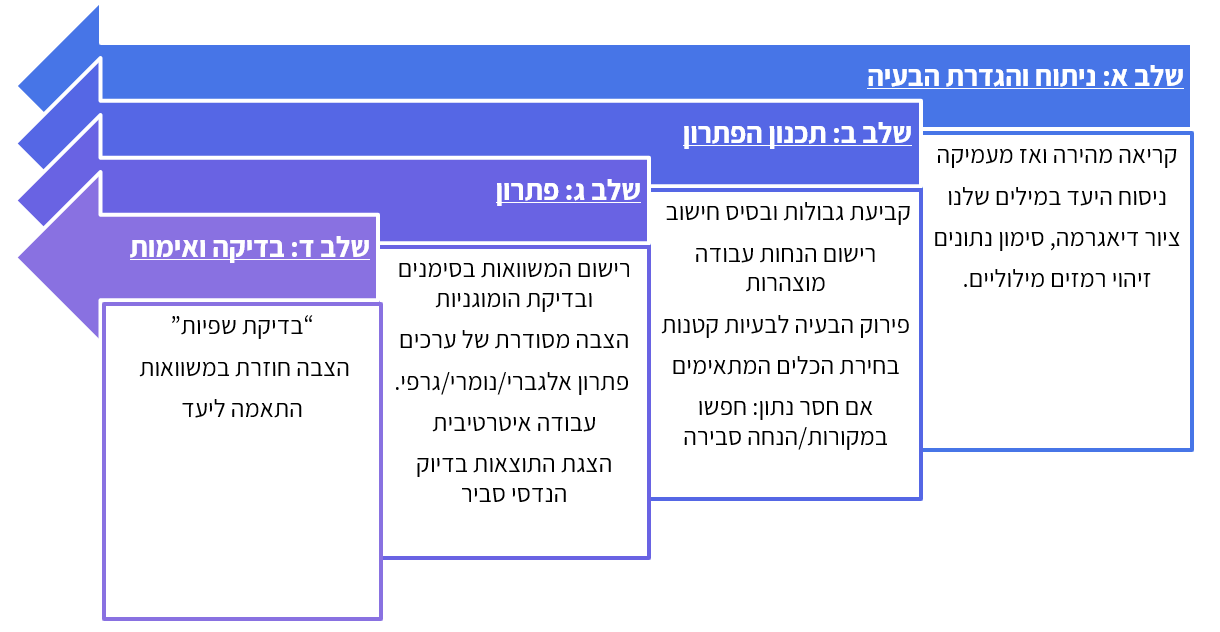
\includegraphics[width=6.5in,height=3.36736in]{media/media/image1.png}

Figure {1 - שלבים בפתרון בעיות}

\subsection{\texorpdfstring{{פתרון בעיות כמיומנות
נרכשת}}{פתרון בעיות כמיומנות נרכשת}}\label{ux5e4ux5eaux5e8ux5d5ux5df-ux5d1ux5e2ux5d9ux5d5ux5ea-ux5dbux5deux5d9ux5d5ux5deux5e0ux5d5ux5ea-ux5e0ux5e8ux5dbux5e9ux5ea}

{מעבר לגישות, חשוב לזכור כי פתרון בעיות הוא מיומנות שמתפתחת עם תרגול.
הטעויות הן החלק הכי חשוב בלמידה. הן מאפשרות לנו להבין היכן ההנחות לא היו
נכונות, היכן המודל לא התאים, או אילו נתונים נדרשו ולא נלקחו בחשבון}.
{כאשר פתרון מצליח מיד, אנו נוטים לעבור הלאה מבלי לשים לב מדוע הוא הצליח.
דווקא כאשר מתרחשת טעות אנו נדרשים לעצור, לנתח את מקור הבעיה, ולהבין את
המגבלות של דרך החשיבה שלנו. במובן זה,}

\begin{tcolorbox}[enhanced jigsaw, colback=white, arc=.35mm, coltitle=black, breakable, toptitle=1mm, leftrule=.75mm, colbacktitle=quarto-callout-note-color!10!white, opacitybacktitle=0.6, bottomtitle=1mm, titlerule=0mm, opacityback=0, colframe=quarto-callout-note-color-frame, title=\textcolor{quarto-callout-note-color}{\faInfo}\hspace{0.5em}{הערה}, rightrule=.15mm, bottomrule=.15mm, toprule=.15mm, left=2mm]

{טעות היא לא כישלון אלא מקור לתובנות חדשות}

\end{tcolorbox}

{היא מאלצת אותנו לשכלל את המיומנות, ומביאה אותנו לפתרונות עמוקים
ויצירתיים יותר}. {יכולת ההנדסה אינה נמדדת רק בפתרון "נכון", אלא גם (שלא
לומר, בעיקר) ביכולת להסביר למה פתרון מסוים שגוי, ולשפר אותו}.

{חשוב לזכור שפתרון בעיות זהו תהליך אינטראקטיבי ולא לינארי, התהליך כולל
שלבים של זיהוי הבעיה, פירוק לגורמים, שילוב ידע מתמטי וכימי, ו"בדיקת
שפיות" (בדיקה של סבירות הפתרון המתקבל). אך מעבר לכך יש שונות מאוד גדולה
בין המערכות השונות והדרכים להתמודד איתן. המטרה היא לפתח דרך מתודית
להתמודדות עם בעיות חדשות ולזהות באילו שלבים אנו נתקעים. תהליך זה כולל
שלבים כמו זיהוי הבעיה, הבנתה, שליפת מידע רלוונטי, סינתזה של הנתונים,
והערכת התוצאה תוך בדיקת יחידות, סדרי גודל ורמת הדיוק הנדרשת.}

\subsubsection{\texorpdfstring{{אימות התוצאות}(validating
results){}}{אימות התוצאות(validating results)}}\label{ux5d0ux5d9ux5deux5d5ux5ea-ux5d4ux5eaux5d5ux5e6ux5d0ux5d5ux5eavalidating-results}

{יש שלוש דרכים עיקריות לבצע אימות כזה}:

\begin{enumerate}
\def\labelenumi{\arabic{enumi}.}
\item
  \textbf{{הצבה חוזרת} (Back-Substitution)} -- {לאחר מציאת הפתרון,
  מציבים אותו בחזרה במשוואות המקוריות ובודקים אם הוא אכן מקיים אותן}.
  {זוהי דרך ישירה לוודא שהפתרון מתמטי תקין}.
\item
  \textbf{{בדיקת סדר גודל} (Order of Magnitude Estimation)} -- {מבצעים
  חישוב גס עם מספרים פשוטים או חזקות של 10 כדי להעריך את גודל התוצאה
  הצפוי}. {אם התוצאה המדויקת שונה בסדרי גודל -- סביר שנפלה טעות. אם היא
  קרובה -- זה נותן ביסוס לתוצאה שלא התרחקנו מהאמת}.
\item
  \textbf{{מבחן ההיגיון} (Test of Reasonableness)} -- {שואלים האם התוצאה
  אפשרית פיזיקלית: האם היא עומדת בתחומי המציאות}? {לדוגמה, אם קיבלנו
  טמפרטורה גבוהה מהשמש או מהירות גדולה ממהירות האור -- יש לשוב ולבדוק את
  הדרך}.
\end{enumerate}

{בדיקה עצמית היא אחת מאבני היסוד של החשיבה ההנדסית}. {מהנדס או מהנדסת
טובים אינם רק פותרים בעיות -- הם גם יודעים לזהות מתי הפתרון שלהם לא סביר
ולתקן בהתאם}.

\subsubsection{\texorpdfstring{{מחסומים בפתרון בעיות: זיהוי וכלים
להתמודדות}}{מחסומים בפתרון בעיות: זיהוי וכלים להתמודדות}}\label{ux5deux5d7ux5e1ux5d5ux5deux5d9ux5dd-ux5d1ux5e4ux5eaux5e8ux5d5ux5df-ux5d1ux5e2ux5d9ux5d5ux5ea-ux5d6ux5d9ux5d4ux5d5ux5d9-ux5d5ux5dbux5dcux5d9ux5dd-ux5dcux5d4ux5eaux5deux5d5ux5d3ux5d3ux5d5ux5ea}

{במקרים רבים סטודנטים וסטודנטיות נתקלים בקשיים שונים בתהליך הפתרון --
לעיתים בשל חוסר ידע, אך לרוב בשל עבודה לא שיטתית. טעויות שכיחות כוללות
קריאה שטחית של השאלה, בחירת משוואות לא מתאימות, בלבול ביחידות, או
חישובים מרושלים. לעיתים הקושי נובע ממתח ולחץ, או ממחשבה חד-כיוונית
שמובילה להיתקעות בפתרון אחד בלבד. ההתקדמות בלמידה מתחילה בזיהוי הסיבה
האמיתית לקושי -- האם מדובר בבעיה בהבנת הנתונים, בתכנון הדרך, או בהערכת
התוצאה -- ורק אז ניתן לשפר את המיומנות המתאימה.}

{כדי להתגבר על מחסומים בפתרון בעיות חשוב לפתח הרגלי חשיבה יעילים: לקרוא
את השאלה כמה פעמים ולנסח אותה במילים שלנו, לצייר דיאגרמה מסודרת של
הנתונים, לתכנן מראש את דרך הפתרון ולחזות תוצאה סבירה. בתחילת הדרך אנו
נעבוד עם מערכות פשוטות כך שעלולה להווצר נטייה לדלג על שלבים, חשוב לזכור
שהמטרה היא לא הפתרון של המערכת הספציפית, אלא פיתוח שיטות להתמודדות עם
מערכות מסובכות יותר בעתיד, ועל כן הדגש הוא על שימוש נכון בשיטות ולא על
התוצאה הסופית.}

\section{\texorpdfstring{{סיכום}}{סיכום}}\label{ux5e1ux5d9ux5dbux5d5ux5dd}

{הנדסת תהליך היא תחום רחב שמאחד עקרונות מדעיים, שיקולים הנדסיים וכלכלה
יישומית לכדי מסגרת אחת. היא גשר בין מעבדה לתעשייה, בין רעיונות חדשניים
ליישום בקנה מידה גדול. המהות שלה היא היכולת להמיר ידע לכדי תהליך מתוכנן
-- כזה שמשרת את החברה, מייצר ערך כלכלי, ושומר על בטיחות האדם והסביבה}.

{\hfill\break
}

\bookmarksetup{startatroot}

\chapter{\texorpdfstring{{מבוא לחישובים
הנדסיים}}{מבוא לחישובים הנדסיים}}\label{ux5deux5d1ux5d5ux5d0-ux5dcux5d7ux5d9ux5e9ux5d5ux5d1ux5d9ux5dd-ux5d4ux5e0ux5d3ux5e1ux5d9ux5d9ux5dd}

\section{\texorpdfstring{{מה נלמד בפרק
הזה}?}{מה נלמד בפרק הזה?}}\label{ux5deux5d4-ux5e0ux5dcux5deux5d3-ux5d1ux5e4ux5e8ux5e7-ux5d4ux5d6ux5d4}

\begin{itemize}
\item
  {\textbf{להמיר} גדלים פיזיקליים בין מערכות יחידות שונות בעזרת מקדמי
  המרה}.
\item
  {\textbf{לזהות} יחידות מקובלות למסה ולמשקל במערכות} SI, CGS
  {ואמריקאיות}; {\textbf{לחשב} משקל מתוך מסה ביחידות טבעיות או מוגדרות}.
\item
  {\textbf{לקבוע} מספר ספרות משמעותיות בערך נתון}; {\textbf{להחיל} כללים
  לקביעת ספרות משמעותיות בתוצאות של פעולות חשבון}.
\item
  {\textbf{לאמת} פתרון באמצעות הצבה חוזרת, בדיקת סדרי גודל ובחינת
  סבירות}.
\item
  {\textbf{לחשב} ממוצע, טווח, שונות וסטיית תקן מנתוני מדגם,
  ו\textbf{לפרש} את משמעותם}.
\item
  {\textbf{להסביר} את עקרון ההומוגניות הממדית של משוואות ו\textbf{להחיל}
  אותו על איברים לא ידועים}.
\item
  {\textbf{לבצע} אינטרפולציה ליניארית בין נתוני טבלה, ו\textbf{לנתח}
  מצבים שבהם השיטה עלולה להטעות}.
\item
  {\textbf{לגזור} משוואת קו ישר משתי נקודות נתונות, ו\textbf{להתאים} קו
  ישר לנתונים ניסיוניים}.
\item
  {\textbf{לזהות} ייצוגים גרפיים מתאימים (רגיל, חצי-לוגריתמי, לוגריתמי)
  עבור קשרים מסוג חזקה או אקספוננט}; {\textbf{לקבוע} פרמטרים מתוך גרף
  ליניארי}.
\end{itemize}

\section{\texorpdfstring{{מימדים
ויחידות}}{מימדים ויחידות}}\label{ux5deux5d9ux5deux5d3ux5d9ux5dd-ux5d5ux5d9ux5d7ux5d9ux5d3ux5d5ux5ea}

{כל תחום המדע וההנדסה בנוי על היכולת שלנו \textbf{לתאר תופעות באופן
מספרי ומדויק}}. {ברגע שאנחנו מתארים תופעה באמצעות מספר ויחידה, אנחנו
יכולים להשוות אותה לתופעות אחרות, לחשב חישובים מתמטיים, לבצע ניבויים ואף
לתכנן מערכות מורכבות. אבל כדי שכל זה יעבוד, עלינו להשתמש בשפה משותפת --
שפה של יחידות ומימדים}.

{אי-הבנה או חוסר הקפדה בהמרת יחידות עלול להוביל לשגיאות חמורות. דוגמה
מפורסמת לכך היא תאונת ה-}\emph{Gimli Glider}{, טיסה של חברת אייר קנדה
שבה המטוס המריא עם חצי מכמות הדלק הדרושה, עקב בלבול בין ליטרים לבין
פאונדים. חוסר תשומת לב לשאלה באיזו יחידת מידה מבטאים את כמות הדלק כמעט
הסתיים באסון. המקרה הזה מדגים עד כמה חיוני להבין היטב מהי מדידה ואיך
מבצעים המרה נכונה בין יחידות}.

\subsection{\texorpdfstring{{מהי
מדידה}?}{מהי מדידה?}}\label{ux5deux5d4ux5d9-ux5deux5d3ux5d9ux5d3ux5d4}

{מדידה היא אחת הפעולות הבסיסיות ביותר במדע ובהנדסה. כאשר אנו מבצעים
מדידה, אנו מבקשים לקבוע כמה גדול מאפיין מסוים של תופעה או עצם, ולבטא את
התוצאה בצורה מספרית. במילים אחרות}, \textbf{{מדידה היא תהליך של השוואת
גודל פיזיקלי ליחידת מידה מוסכמת, והבעת התוצאה במספר וביחידה}}.

{כדי להבין טוב יותר, כדאי להבחין בין שלושת המושגים}:

\textbf{{מידה} (Quantity):} {התכונה הפיסיקלית שניתנת למדידה ולהשוואה,
כמו מסה, אורך, לחץ, טמפרטורה או הספק.}

\textbf{{מימד} (Dimension):} {המאפיין הפיזיקלי הבסיסי של אותה מידה--
למשל אורך, מסה, זמן,} {או שילובים שלהם (למשל אורך ליחידת זמן). הממד מתאר
את סוג הגודל הפיזיקלי הנמדד.}

\textbf{{יחידה} (Unit):} {קנה המידה שבו משתמשים כדי לבטא את הממד. למשל,
אורך אפשר למדוד במטרים, סנטימטרים או אינצ'ים. זמן אפשר למדוד בשניות,
דקות או שעות}.

{לדוגמה: אם נאמר שהתאוצה היא} \(10\frac{m}{s^{2}}\) {, המידה היא התאוצה,
המימדים הם אורך ליחידת זמן בריבוע, והיחידות הן מטר לשנייה בריבוע.}

{חשוב לשים לב להבדל בין מימד ליחידה}:

\begin{tcolorbox}[enhanced jigsaw, colback=white, arc=.35mm, coltitle=black, breakable, toptitle=1mm, leftrule=.75mm, colbacktitle=quarto-callout-note-color!10!white, opacitybacktitle=0.6, bottomtitle=1mm, titlerule=0mm, opacityback=0, colframe=quarto-callout-note-color-frame, title=\textcolor{quarto-callout-note-color}{\faInfo}\hspace{0.5em}{הערה}, rightrule=.15mm, bottomrule=.15mm, toprule=.15mm, left=2mm]

\begin{itemize}
\tightlist
\item
  {\textbf{המימד} עונה על השאלה \emph{מה אנחנו מודדים}} -- {אורך, זמן,
  מסה, טמפרטורה}.
\item
  {\textbf{היחידה} עונה על השאלה מהו הגודל המוסכם אליו אנו משווים -}
  {מטרים, שניות, קילוגרמים, מעלות צלזיוס}.
\end{itemize}

\end{tcolorbox}

\subsection{\texorpdfstring{{יחידות מידה -- מסע קצר
בהיסטוריה}}{יחידות מידה -- מסע קצר בהיסטוריה}}\label{ux5d9ux5d7ux5d9ux5d3ux5d5ux5ea-ux5deux5d9ux5d3ux5d4-ux5deux5e1ux5e2-ux5e7ux5e6ux5e8-ux5d1ux5d4ux5d9ux5e1ux5d8ux5d5ux5e8ux5d9ux5d4}

{לפני שהיה סטנדרט בינלאומי, כל תרבות השתמשה ביחידות שונות. רבות מהן היו
מבוססות על גוף האדם או על צורכי היומיום. למשל}:

\begin{itemize}
\item
  \textbf{{אמה} (Cubit):} {המרחק מהמרפק עד קצה האצבעות, ששימש במצרים
  העתיקה לבנייה}.
\item
  \textbf{פאתום (Fathom):} אורך של שישה צעדי רגל, בערך ‎1.8‎ מטר, ששימש
  למדידת עומק מים.
\item
  \textbf{מיל רומי (Roman Mile):} מקור השם \emph{מייל} הוא מהמילה
  הלטינית \emph{mille passus} --- כלומר ``אלף צעדים''.\\
  אצל הרומאים צעד נחשב לשני פסיעות (צעד שמאל וצעד ימין יחד), ולכן המיל
  הרומי היה שווה לאלף זוגות צעדים --- בערך ‎1480‎ מטר.\\
  יחידת מדידה זו שימשה את הלגיונות הרומיים לסימון דרכים ונשארה בסיס לחלק
  מהיחידות שהתפתחו מאוחר יותר באירופה.
\item
  \textbf{{מייל ימי}:} {כ-1.852 ק"מ, נבעה מחיבור בין מפות הכוכבים
  למרחקים על פני הים, באמצעות מדידות סקסנט ומחישובים של הימאים. היום
  מייל ימי מוגדר כ"דקת קשת" המרחק שמקבלים כאשר מחלקים את היקף כדור הארץ
  ל360 מעלות ו60 דקות בכל מעלה.}
\item
  \textbf{{סמאוט} (Smoot):} {יחידת מידה הומוריסטית שהומצאה ב}MIT {ושווה
  לאורך גופו של סטודנט בשם אוליבר סמאוט (כ}-{1.70 מ\textquotesingle)}.
\end{itemize}

{יחידות אלו אולי נראות לנו מוזרות או מגוחכות היום, אך הן היו הגיוניות
בתקופתן. היתרון הגדול בשימוש ביחידות המבוססות על גוף האדם הוא נוחות
וזמינות: לכל אחד יש יד, רגל או אמה, ולכן לא צריך כלי מדידה מיוחד כדי
לקבוע מרחקים או גדלים. כך למשל, חקלאי יכול היה למדוד שדה בצעדים, ובנאי
יכול היה למדוד קורות לפי אמות ידיו. עם זאת, יחידות כאלו סובלות מבעיה
מרכזית -- הן אינן אחידות. אורך הזרוע של אדם אחד שונה מזה של אחר, ואפילו
אצל אותו אדם המדידה אינה מדויקת לאורך זמן. חוסר האחידות הזה מקשה מאוד על
תקשורת מדעית וטכנית: מה שאצל אחד הוא "אמה" של 45 ס"מ יכול אצל אחר להיות
50 ס"מ. לכן, ככל שהמדע והטכנולוגיה התקדמו, התעורר צורך ביחידות מוסכמות,
קבועות ומוגדרות היטב. השימוש ביחידות בינלאומיות מאפשר לנו לתקשר ידע
בצורה אמינה וברורה, לבצע חישובים עקביים, ולמנוע טעויות שנובעות מפרשנויות
שונות של אותה מידה}.

\subsection{\texorpdfstring{{מעבר בין
יחידות}}{מעבר בין יחידות}}\label{ux5deux5e2ux5d1ux5e8-ux5d1ux5d9ux5df-ux5d9ux5d7ux5d9ux5d3ux5d5ux5ea}

{הצורך ביחידות מוסכמות אינו נובע רק מהיסטוריה של בלבול או נוחות, אלא מכך
שאין כל משמעות פיזיקלית לחיבור בין גדלים מימדים שונים}. {אי אפשר לחבר
שלושה מטרים לחמש שניות, משום שמדובר בגדלים השייכים לקטגוריות שונות
לגמרי. כמו כן, כאשר עובדים עם אותו מימד אפשר לבצע חיבור והשוואה -- אך
ורק אם כל הערכים מבוטאים באותה יחידה. אם הערכים נתונים ביחידות שונות,
למשל מטרים וסנטימטרים, תחילה נמיר את כולם ליחידה אחידה ורק אז נוכל לחבר
או להשוות ביניהם. רק כאשר כל הגדלים באותו ממד ובאותה יחידה, ניתן לבצע
פעולות של חיבור, חיסור והשוואה בין ערכים.}

{מצד שני, בעוד שחיבור וחיסור אפשריים רק כאשר מדובר באותו ממד ובאותה
יחידה (או לאחר המרה ליחידה אחידה), הרי שבכפל ובחילוק היחידות מתנהגות ממש
כמו גורמים אלגבריים: ניתן להכפיל אותן, לחלק אותן ואף לצמצם ביניהן}.
{בצורה זו אנו יכולים לעבור בין יחידות שונות באותו מימד, ואף ליצור יחידות
חדשות המייצגות גדלים פיזיקליים חדשים.}

{במילים פשוטות}

\begin{tcolorbox}[enhanced jigsaw, colback=white, arc=.35mm, coltitle=black, breakable, toptitle=1mm, leftrule=.75mm, colbacktitle=quarto-callout-tip-color!10!white, opacitybacktitle=0.6, bottomtitle=1mm, titlerule=0mm, opacityback=0, colframe=quarto-callout-tip-color-frame, title=\textcolor{quarto-callout-tip-color}{\faLightbulb}\hspace{0.5em}{עצה}, rightrule=.15mm, bottomrule=.15mm, toprule=.15mm, left=2mm]

\begin{itemize}
\tightlist
\item
  {אי אפשר לחבר גדלים ממימדים שונים:}
  \(1\text{ }m + 3\text{ }L = \text{undefined}\)❌
\item
  {אפשר לחבר רק כשיש אותו מימד ואותה יחידה:}
  \(10\text{ }cm + 5\text{ }cm = 15\text{ }cm\)✅
\item
  {אם היחידות שונות -- חייבים להמיר:}
  \(10\text{ }m + 20\text{ }ft = ?\){← המרה ליחידה אחידה}
\item
  {בכפל ובחילוק היחידות מתנהגות כמו ביטוי אלגברי:}

  \begin{itemize}
  \tightlist
  \item
    {ניתן להכפיל, לחלק ולצמצם יחידות} {באותו המימד}
  \item
    {בצורה זו ניתן להגדיר יחידות נגזרות (כוח, אנרגיה, לחץ).}
  \end{itemize}
\end{itemize}

\end{tcolorbox}

{המהירות מוגדרת על ידי חלוקת המרחק בזמן ולכן}

\[\frac{30km}{3h} = 10\frac{km}{h}\]

{אלו הן יחידות נגזרות, ואנו נדון בהן בהרחבה בהמשך הפרק.}

{על מנת לעבור מיחידה אחת ליחידה אחרת, נשתמש בפקטור מעבר}

{פקטור מעבר} \textbf{(Conversion Factor) {}}{-\\
יחס בין שתי יחידות השייכות לאותו המימד ומייצגות את אותה הכמות.}

{זהו יחס מתמטי בין שתי יחידות של אותו ממד, שמבחינה פיסיקלית שווה ל}-{1.
פקטור המעבר מאפשר לשנות את היחידות מבלי לשנות את הגודל עצמו}.

\[1m = 100cm\  \rightarrow \ \ \frac{1m}{100cm}\ \ \ \ \ or \ \ \ \ \frac{100cm}{1m}\]

\[1h = 3600s\  \rightarrow \ \ \ \ \frac{1h}{3600s}\ \ \ \ \ or \ \ \ \frac{3600s}{1h}\]

{כאשר נכפיל גודל פיזיקלי בפקטור מעבר}, \textbf{{המספר ישתנה, היחידות
יתעדכנו, אבל הגודל הפיזיקלי עצמו יישאר זהה}}. {לדוגמה, אם נאמר שאורך
מסוים הוא 1.5 מטר, אפשר לבטא אותו גם כ}-{150 סנטימטר -- שתי הצורות
נכונות, והגודל האמיתי לא השתנה}. {היחסים בין הגדלים השונים הם קבועים
וניתן למצוא אותן בספרים.}

Figure {2 - גדלים לצורך העברת יחידות. הטבלה מתוך }Felder, R.M.,
Rousseau, R.W., \& Bullard, L.G. (2016). Elementary Principles of
Chemical Processes (4th ed.). Wiley

{השתמשו בטבלה על מנת להגדיר את פקטורי המעבר הבאים}

\begin{itemize}
\item
  {ליטר לגלון (}L-\textgreater gal{)}
\item
  {מטר לפיט (}m-\textgreater ft{)}
\end{itemize}

{כעת נוכל להשתמש בפקטור המעבר על מנת לפתור את המשוואה}
\[10m + 20ft = ?\] {לצורך כך נמצא את פקטור המעבר בין מטר לפיט. על פי
הטבלה} 1m=3.28ft {ולכן נוכל להגדיר את פקטורי המעבר}
\[\frac{1m}{3.28ft}\ \ \ \ \ or\ \ \ \frac{3.28ft}{1m}\] {וכך נוכל לחשב}
\[20ft\  \times \frac{1m}{3.028ft} = 6.1m\]

{שימו לב שניתן לצמצם את היחידות הישנות כך שאנו נשארים רק עם היחידות
החדשות.}

{בתחום שלנו נהוג לכתוב מעבר זה באמצעות שימוש \textbf{בסרגל מעבר יחידות}
הנראה כך}

\begin{enumerate}
\def\labelenumi{\arabic{enumi}.}
\item
  {הוא מאפשר לנו לראות בצורה יותר ברורה שלא נעשתה טעות במעבר היחידות.\\
  אם בטעות היינו כותבים}
\end{enumerate}

{היינו רואים שהיחידות לא מצטמצמות כפי שרצינו ומתקנים את ההצבה}

\begin{enumerate}
\def\labelenumi{\arabic{enumi}.}
\setcounter{enumi}{1}
\item
  הוא מאפשר לנו לשרשר מספר מעברי יחידות אחד אחרי השני, ללא חישובי ביניים
  כך שהסיכוי לטעות חישובית במהלך המעברים מצטמצם משמעותית.\\
  כך למשל, אם נרצה לעבור מיחידות של \textbf{ft/h} ליחידות של
  \textbf{m/min}, נגדיר את פקטורי המעבר הנדרשים באמצעות הטבלה:

  \[
  \frac{1h}{60min} \quad \text{or} \quad \frac{60min}{1h} \quad ; \quad \frac{1m}{3.28ft} \quad \text{or} \quad \frac{3.28ft}{1m}
  \]
\end{enumerate}

\textbf{{שימוש בסרגל יחידות הוא כלי מרכזי להמרות נכונות ולמניעת
טעויות}\emph{.}} {השיטה מחייבת להציב את הכמות הנתונה בצד שמאל, ולצידה
סדרה של גורמי המרה הכתובים כשברים. כל גורם נבחר כך שיבטל את היחידות הלא
רצויות ויחליף אותן ביחידות המבוקשות. ברגע שמציבים את היחידות בתוך השברים
ומצמצמים אותן באופן אלגברי, נותרת בסוף רק היחידה הרצויה}\emph{.}

{חשוב להכיר בכך שזו אינה שיטה אינטואיטיבית עבור רוב הסטודנטים בתחילת
הדרך: בהתחלה היא עשויה להיראות מסורבלת או מלאכותית. עם זאת, לאחר
שמתרגלים לעבוד כך, מתגלה יתרון גדול -- לא רק שהשיטה כמעט מבטלת טעויות
בסיסיות, אלא היא גם מספקת כלי להתמודדות עם מצבים חדשים ולא מוכרים. כאשר
מופיעה בעיה שלא ראינו בעבר, עצם העבודה עם היחידות מובילה אותנו בצעדים
מסודרים אל הפתרון}\emph{.}

{משאית נסעה מרחק של} 25mile {במשך 20 דקות. מהי המהירות של המשאית במטר
לשנייה?}

\subsection{\texorpdfstring{{סיכום}}{סיכום}}\label{ux5e1ux5d9ux5dbux5d5ux5dd-1}

{בפרק זה הכרנו את המושגים הבסיסיים של עולם המדידה:}

\begin{itemize}
\item
  {\textbf{מדידה} (}measurement{) היא פעולה של השוואת גודל ליחידת מידה
  מוסכמת.}
\item
  {\textbf{מידה} (}quantity{) היא תכונה פיסיקלית אותה ניתן לכמת.}
\item
  {\textbf{מימד} (}dimention{) הוא סוג הגודל (אורך, מסה, זמן...).}
\item
  {\textbf{יחידה} (}unit{) היא קנה המידה (מטר, קילוגרם, שנייה).}
\item
  {\textbf{פקטור מעבר} (}conversion factor{) הוא יחס בין שתי יחידות
  השייכות לאותו המימד ומייצגות את אותה הכמות}
\end{itemize}

{בנוסף למדנו גם כיצד לבצע המרות באמצעות \textbf{סרגל היחידות} (}simple
dimensional analysis{). שיטה זו מבטיחה עבודה עקבית עם היחידות, מונעת
טעויות נפוצות ומסייעת להבין מצבים חדשים ולא מוכרים.}

\section{\texorpdfstring{{מערכות
יחידות}}{מערכות יחידות}}\label{ux5deux5e2ux5e8ux5dbux5d5ux5ea-ux5d9ux5d7ux5d9ux5d3ux5d5ux5ea}

מערכת יחידות היא מסגרת מוסכמת של יחידות בסיס ונגזרות, המאפשרת למדוד
ולחשב גדלים פיזיקליים בצורה עקבית. כל מערכת יחידות מורכבת משלושה מרכיבים
-- יחידות בסיס, יחידות מרובות, ויחידות נגזרות.\\
בעולם המדע וההנדסה נעשה שימוש בכמה מערכות יחידות שונות. המערכת המרכזית
והמוסכמת כיום היא \textbf{המערכת הבינלאומית (SI)}, המבוססת על המטר,
הקילוגרם והשנייה, והיא המערכת הרשמית ברוב מדינות העולם.\\
לצד ה־\textbf{SI} קיימת גם \textbf{מערכת ה־CGS}, שהייתה נפוצה יותר בעבר
ובה יחידות הבסיס הן הסנטימטר, הגרם והשנייה. בארצות הברית מקובלת בעיקר
\textbf{המערכת האמריקאית (American Engineering System -- AES)}, שבה
יחידות הבסיס הן הרגל, הפאונד־מסה והשנייה.\\
ההבדלים בין מערכות אלו מתבטאים בעיקר בבחירת יחידות הבסיס ובמורכבות
ההמרות ביניהן, אך כולן מבוססות על אותם עקרונות של מדידה עקבית.

\subsection{\texorpdfstring{{מידות
בסיסיות}}{מידות בסיסיות}}\label{ux5deux5d9ux5d3ux5d5ux5ea-ux5d1ux5e1ux5d9ux5e1ux5d9ux5d5ux5ea}

ישנן 7 מידות בסיסיות אשר מהוות את המימדים הבסיסיים מהם יוגדרו כל שאר
המידות. בכל מערכות היחידות המידות הבסיסיות הן זהות, אך היחידות בהן
מודדים מידות אלו משתנות. יחידות אלו אינן מוגדרות מתוך יחידות אחרות אלא
מהוות נקודת מוצא מוסכמת למדידה.

\textbf{יחידות בסיס במערכות מדידה שונות}

\begin{longtable}[]{@{}
  >{\centering\arraybackslash}p{(\linewidth - 8\tabcolsep) * \real{0.2000}}
  >{\centering\arraybackslash}p{(\linewidth - 8\tabcolsep) * \real{0.2000}}
  >{\centering\arraybackslash}p{(\linewidth - 8\tabcolsep) * \real{0.2000}}
  >{\centering\arraybackslash}p{(\linewidth - 8\tabcolsep) * \real{0.2000}}
  >{\centering\arraybackslash}p{(\linewidth - 8\tabcolsep) * \real{0.2000}}@{}}
\toprule\noalign{}
\begin{minipage}[b]{\linewidth}\centering
\textbf{מידה}
\end{minipage} & \begin{minipage}[b]{\linewidth}\centering
\textbf{ביטוי מימדי}
\end{minipage} & \begin{minipage}[b]{\linewidth}\centering
\textbf{SI{(סימן / שם)}}
\end{minipage} & \begin{minipage}[b]{\linewidth}\centering
\textbf{CGS{(סימן / שם)}}
\end{minipage} & \begin{minipage}[b]{\linewidth}\centering
\textbf{AES{(סימן / שם)}}
\end{minipage} \\
\midrule\noalign{}
\endhead
\bottomrule\noalign{}
\endlastfoot
אורך & {[}L{]} & mmeter & cmcentimeter & ftfoot \\
מסה & {[}M{]} & kgkilogram & ggram & lbₘpound \\
זמן & {[}T{]} & ssecond & ssecond & ssecond \\
טמפרטורה & {[}Θ{]} & Kkelvin & Kkelvin & °Ffahrenheit \\
זרם חשמלי & {[}I{]} & Aampere & Aampere & Aampere \\
כמות חומר & {[}N{]} & molmole & molgram-mole & lb-molpound-mole \\
עוצמת אור & {[}J{]} & Cdcandela & Cdcandela & Cdcandela \\
\end{longtable}

Figure {3} - {היחידות הבסיסיות עבור כל מערכת יחידות}

\subsection{\texorpdfstring{{יחידות
מרובות}}{יחידות מרובות}}\label{ux5d9ux5d7ux5d9ux5d3ux5d5ux5ea-ux5deux5e8ux5d5ux5d1ux5d5ux5ea}

{\textbf{יחידות מרובות} הן יחידות שמוגדרות כשבר או כמכפלה של יחידות
בסיס. לדוגמא -- יחידת הבסיס של זמן היא שנייה אך אנו נוהגים להתייחס לזמן
גם בדקות, שעות, ימים או שנים. מבחינה עקרונית כל גודל פיסיקלי ניתן להביע
ביחידות הבסיס עצמן, אך הדבר אינו נוח: מה היה קורה לו היינו צריכים
וצריכות לתאר את הגיל שלנו בשניות?} {לכן, יחידות מרובות משמשות אותנו לא
מתוך הכרח מתמטי אלא כדי לאפשר הצגה יעילה ונוחה יותר של כמויות גדולות או
קטנות במיוחד}.

דוגמאות לכך ניתן למצוא בכל מערכת יחידות: את משקל המשאית ב SI אנו נעדיף
לתאר בטונות (Ton) ולא בק"ג, ואת המרחק בין ישראל ללונדון ב AES נתאר במייל
(mile) ולא ברגל (ft).

שיטה נוספת לייצוג פשוט של גדלים פיזיקליים היא באמצעות שימוש בקידומות
(prefixes), אשר מהוות דרך נוחה להציג ערכים גדולים או קטנים מאוד מבלי
להכביד במספרים ארוכים. כל קידומת מייצגת מכפלה או שבר של יחידת הבסיס,
והיא נצמדת לסימול היחידה עצמה.

לדוגמה, הקידומת k (קילו) מציינת מכפלה של \(10^3\) -- כלומר אלף יחידות:
\(1~\text{km} = 1000~\text{m}\)  \(1~\text{kg} = 1000~\text{g}\)  \(1~\text{kJ} = 1000~\text{J}\)

באופן דומה, הקידומת μ (מיקרו) מציינת שבר של \(10^{-6}\) -- כלומר
מיליונית מהיחידה:
\(1~\text{μm} = 10^{-6}~\text{m}\)  \(1~\text{μs} = 10^{-6}~\text{s}\)  \(1~\text{μL} = 10^{-6}~\text{L}\)

השימוש בקידומות התפתח במסגרת מערכת ה־SI, אך כיום הן מקובלות גם במערכות
יחידות אחרות, כגון AES, ולכן הפכו לסטנדרט אוניברסלי. עבור מהנדסים
ומהנדסות, שליטה בקידומות אלו חיונית, שכן הן כלי מרכזי להצגה מדויקת,
קריאה ויעילה של נתונים מדעיים והנדסיים.

Figure {4 - קידומות מוכרים ליחידות, מתוך }García, José. (2025).
Dimensional Analysis in Chemistry Textbooks 1900-2020 and an Algebraic
Alternative. Educación Química. 36. 82-108.
10.22201/fq.18708404e.2025.1.88260

{השלימו באמצעות טבלת הקידומות} \[\begin{matrix}
\mathbf{1}\mathbf{Mg} & = & \_\_\_\_\_\_\_\_\_\_\mathbf{g}\_\_ \\
\_\_\_\_\_\_\_\_\_\_\_\_\_\_ & = & \mathbf{1.5*1}\mathbf{0}^{\mathbf{- 6}}\mathbf{s} \\
\mathbf{1}\mathbf{nm} & & \_\_\_\_\_\_\_\_\_\_\_\_\_\mathbf{m}
\end{matrix}\]

\subsection{\texorpdfstring{{יחידות
נגזרות}}{יחידות נגזרות}}\label{ux5d9ux5d7ux5d9ux5d3ux5d5ux5ea-ux5e0ux5d2ux5d6ux5e8ux5d5ux5ea}

יחידות נגזרות הן יחידות שמתקבלות משילוב מתמטי של יחידות הבסיס ---
באמצעות כפל או חילוק. בעוד יחידות הבסיס נבחרות כמוסכמות בינלאומיות שאינן
תלויות זו בזו, יחידות נגזרות מתארות גדלים פיזיקליים מורכבים יותר, כמו
מהירות, תאוצה, כוח, אנרגיה ולחץ.

יחידות נגזרות הן ביטוי מתמטי פשוט של יחידות הבסיס. כך למשל, מהירות נמדדת
במטר לשנייה (\(m/s\)), תאוצה במטר לשנייה בריבוע (\(m/s^{2}\)), כוח
בניוטון (\(N = kg \cdot m/s^{2}\)), ואנרגיה בג׳אול
(\(J = kg \cdot m^{2}/s^{2}\)).

טבלה זו מדגימה כיצד כל גודל פיזיקלי מורכב מתפרק תמיד לשילוב של המידות
היסודיות: במקרים אלו - מסה, אורך וזמ {כך לדוגמא במערכת} SI

\begin{longtable}[]{@{}
  >{\centering\arraybackslash}p{(\linewidth - 8\tabcolsep) * \real{0.2000}}
  >{\centering\arraybackslash}p{(\linewidth - 8\tabcolsep) * \real{0.2000}}
  >{\centering\arraybackslash}p{(\linewidth - 8\tabcolsep) * \real{0.2000}}
  >{\centering\arraybackslash}p{(\linewidth - 8\tabcolsep) * \real{0.2000}}
  >{\centering\arraybackslash}p{(\linewidth - 8\tabcolsep) * \real{0.2000}}@{}}
\toprule\noalign{}
\begin{minipage}[b]{\linewidth}\centering
\textbf{גודל פיזיקלי}
\end{minipage} & \begin{minipage}[b]{\linewidth}\centering
\textbf{סימול יחידה}
\end{minipage} & \begin{minipage}[b]{\linewidth}\centering
\textbf{יחידה}
\end{minipage} & \begin{minipage}[b]{\linewidth}\centering
\textbf{ביטוי ביחידות בסיס}
\end{minipage} & \begin{minipage}[b]{\linewidth}\centering
\textbf{ביטוי במימדים}
\end{minipage} \\
\midrule\noalign{}
\endhead
\bottomrule\noalign{}
\endlastfoot
מהירות & \(m/s\) & מטר לשנייה & \(m/s\) &
\([\mathbf{L}]/[\mathbf{T}]\) \\
תאוצה & \(m/s^2\) & מטר לשנייה² & \(m/s^2\) &
\([\mathbf{L}]/[\mathbf{T}]^{\mathbf{2}}\) \\
כוח & \(N\) & ניוטון & \(kg \cdot m/s^2\) &
\([\mathbf{M}]\cdot[\mathbf{L}]/[\mathbf{T}]^{\mathbf{2}}\) \\
אנרגיה & \(J\) & ג'אול & \(kg \cdot m^2/s^2\) &
\([\mathbf{M}]\cdot[\mathbf{L}]^{\mathbf{2}}/[\mathbf{T}]^{\mathbf{2}}\) \\
לחץ & \(Pa\) & פסקל & \(kg/(m \cdot s^2)\) &
\([\mathbf{M}]/([\mathbf{L}]\cdot[\mathbf{T}]^{\mathbf{2}})\) \\
הספק & \(W\) & וואט & \(kg \cdot m^2/s^3\) &
\([\mathbf{M}]\cdot[\mathbf{L}]^{\mathbf{2}}/[\mathbf{T}]^{\mathbf{3}}\) \\
\end{longtable}

{מעבר ליחידות הנגזרות שמוגדרות ישירות מתוך יחידות הבסיס (כמו ניוטון או
ג'אול), קיימות גם \textbf{יחידות מורכבות נוספות} שנקבעו לשימוש נוח יותר
בתחומים שונים. יחידות אלו מבטאות את אותם המימדים הפיזיקליים -- אך בערכים
מספריים נוחים או ביחידות מותאמות למדידות מעשיות}.\\
{כך, למשל, לחץ ניתן למדידה הן ב}-{פסקל} (Pa) {והן ב}-{אטמוספירה} (atm),
{ואנרגיה יכולה להימדד בג'אול} (J) {או בארג} (erg). {הבחירה ביחידה תלויה
בהקשר}: {ניסויי מעבדה, תעשייה או מערכת המדידה הנהוגה, אך כולן שקולות
מבחינת המימדים שהן מייצגות}.

\begin{longtable}[]{@{}
  >{\centering\arraybackslash}p{(\linewidth - 8\tabcolsep) * \real{0.2000}}
  >{\centering\arraybackslash}p{(\linewidth - 8\tabcolsep) * \real{0.2000}}
  >{\centering\arraybackslash}p{(\linewidth - 8\tabcolsep) * \real{0.2000}}
  >{\centering\arraybackslash}p{(\linewidth - 8\tabcolsep) * \real{0.2000}}
  >{\centering\arraybackslash}p{(\linewidth - 8\tabcolsep) * \real{0.2000}}@{}}
\toprule\noalign{}
\begin{minipage}[b]{\linewidth}\centering
\textbf{מערכת}
\end{minipage} & \begin{minipage}[b]{\linewidth}\centering
\textbf{גודל פיזיקלי}
\end{minipage} & \begin{minipage}[b]{\linewidth}\centering
\textbf{שם יחידה}
\end{minipage} & \begin{minipage}[b]{\linewidth}\centering
\textbf{סימול}
\end{minipage} & \begin{minipage}[b]{\linewidth}\centering
\textbf{ערך היחידה}
\end{minipage} \\
\midrule\noalign{}
\endhead
\bottomrule\noalign{}
\endlastfoot
\textbf{SI} & לחץ & אטמוספירה & atm &
\(\mathbf{1\ atm = 101{,}325\ Pa}\) \\
\textbf{SI} & נפח & ליטר & L & \(\mathbf{1\ L = 10^{-3}\ m^{3}}\) \\
\textbf{SI} & מסה & טון & T & \(\mathbf{1\ T = 10^{3}\ kg}\) \\
\textbf{CGS} & כוח & דיין & dyne &
\(\mathbf{1\ dyne = 1\ \frac{g \cdot cm}{s^{2}}}\) \\
\textbf{CGS} & אנרגיה & ארג & erg &
\(\mathbf{1\ erg = 1\ g \cdot cm^{2}/s^{2}}\) \\
\textbf{AES / U.S. customary} & הספק & כוח סוס (Horsepower) & hp &
\(\mathbf{1\ hp \approx 550\ \frac{ft \cdot lb_{f}}{s}}\) \\
\textbf{AES / U.S. customary} & נפח & גלון & Gal &
\(\mathbf{1\ gal \approx 231\ in^{3}}\) \\
\end{longtable}

{מה פקטור המעבר בין} dyne {ל-}N{? חשבו באמצעות יחידות הבסיס.} {(רמז-
התחילו בביטוי ביחידות הבסיס של אחד מהם, והשתמשו במעברי יחידות על מנת
להמיר אותן כך שיתאימו ליחידות הבסיס של השני)}

\subsection{\texorpdfstring{{כוח
ומשקל}}{כוח ומשקל}}\label{ux5dbux5d5ux5d7-ux5d5ux5deux5e9ux5e7ux5dc}

במערכת ה־SI כל יחידות הבסיס הוגדרו כך שהקשרים ביניהן עקביים ומדויקים,
ולכן נגזרות כמו ניוטון או ג׳אול אינן דורשות מקדם תיקון - היחידות
``מסונכרנות'' באופן טבעי. לעומת זאת, במערכת ה־AES יחידות הבסיס אינן
מוגדרות כך, ולכן כאשר מחשבים כוח או גדלים נגזרים אחרים נדרש להשתמש בקבוע
תיקון נומרי (\(g_{c}\)) כדי לשמור על עקביות מימדית.

{נזכר כי מתוך החוק השני של ניוטון אנו יודעים ש}

\[F = ma\]

{במערכת} SI {יחידת הכח הוגדרה כך שהיא שווה מבחינה נומרית למכפלת יחידות
הבסיס המרכיבות אותה.}

\[1N \equiv 1Kg*\frac{m}{s^{2}}\]

{ובאופן דומה במערכת} \emph{CGS} {הוגדרה יחידת הכח} \emph{dyne} {כך ש}

\[1dyne \equiv 1g*\frac{cm}{s^{2}}\]

{לעומת זאת, ביחידות} \emph{AES} {כח של} \(1lb_{f}\) {לא הוגדרה מתוך
יחידות הבסיס אלא הוגדרה היסטורית כמשקלו של פאונד מסה אחד בתנאי כבידה
סטנדרטיים, ז"א}

\[1lbf \equiv 32.174\frac{lb_{m}ft}{s^{2}}\]

{לכן, במערכת היחידות האמריקאית הגדירו מחדש את החוק השני של ניוטון כך ש}

\[F = \frac{ma}{g_{c}}\ \ \ \ \ ;\ \ \ \ \ g_{c} = 32.174\frac{lb_{m}ft}{lb_{f}s^{2}}\]

\subsubsection{\texorpdfstring{יישום חוקי ניוטון ושימוש ב- \(g_c\) (SI
ו-AES)}{יישום חוקי ניוטון ושימוש ב- g\_c (SI ו-AES)}}\label{ux5d9ux5d9ux5e9ux5d5ux5dd-ux5d7ux5d5ux5e7ux5d9-ux5e0ux5d9ux5d5ux5d8ux5d5ux5df-ux5d5ux5e9ux5d9ux5deux5d5ux5e9-ux5d1--g_c-si-ux5d5-aes}

\textbf{מטרת הדוגמה:} להמחיש את השימוש העקבי בחוק השני של ניוטון באמצעות
קבוע ההמרה \(g_c\), ולהראות כיצד הוא מגשר בין יחידות המסה ליחידות הכוח
בכל שיטה.

גוף בעל מסה \(M\) מונח על משטח אופקי חסר חיכוך. תאוצת הכובד המקומית היא
\(g\). עליכם לחשב:

\begin{enumerate}
\def\labelenumi{\arabic{enumi}.}
\tightlist
\item
  \textbf{חישוב סטטי (\(W\)):} כוח הכבידה (המשקל) הפועל על הגוף.
\item
  \textbf{חישוב דינמי (\(a\)):} התאוצה שיקבל הגוף כתוצאה מהפעלת כוח
  אופקי חיצוני \(F\).
\end{enumerate}

בצעו את החישובים עבור שני המקרים הבאים:

\begin{itemize}
\tightlist
\item
  \textbf{מקרה א' (מערכת SI):} המסה \(M=100 \text{ kg}\), תאוצת הכובד
  \(g=9.81 \text{ m/s}^2\), והכוח \(F=500 \text{ N}\).
\item
  \textbf{מקרה ב' (מערכת AES):} המסה \(M=100 \text{ lb}_m\), תאוצת הכובד
  \(g=32.2 \text{ ft/s}^2\), והכוח \(F=50 \text{ lb}_f\).
\end{itemize}

המשוואה הכללית לחוק השני של ניוטון, כאשר המסה מופרדת, היא:

\[
F = M \cdot \frac{a}{g_c}
\]

עבור משקל (\(W\)), התאוצה היא \(g\):

\[
W = M \cdot \frac{g}{g_c}
\]

\emph{חלק א': מערכת יחידות בינלאומית (SI)}

במערכת זו, נהוג לרוב להשמיט את \(g_c\) כי ערכו הוא 1, אך כדי להבין כיצד
היחידות משתנות מקילוגרם לניוטון, נציב אותו במפורש. ערך הקבוע הוא:
\[g_c = 1 \frac{kg \cdot m}{N \cdot s^2}\]

\textbf{1. חישוב המשקל:}

\[
W = 100 \text{ kg} \cdot \frac{9.81 \frac{\text{m}}{\text{s}^2}}{1 \frac{\text{kg} \cdot \text{m}}{\text{N} \cdot \text{s}^2}}
\]

נסדר את היחידות כדי לראות את הצמצום: ה-\(kg\), ה-\(m\) וה-\(s^2\)
מצטמצמים כולם, וה-\(N\) (שנמצא במכנה של המכנה) עולה למונה:

\[
W = 100 \cdot \frac{9.81}{1} \text{ N} = \mathbf{981 \text{ N}}
\]

\textbf{2. חישוב התאוצה:}

נבודד את \(a\) מהמשוואה: \(a = \frac{F \cdot g_c}{M}\)

\[
a = \frac{500 \text{ N} \cdot 1 \frac{\text{kg} \cdot \text{m}}{\text{N} \cdot \text{s}^2}}{100 \text{ kg}}
\]

כאן ניתן לראות בבירור שהניוטון (\(N\)) מצטמצם, והקילוגרם (\(kg\))
מצטמצם, ונותרנו רק עם יחידות תאוצה:

\[
a = \frac{500}{100} \frac{\text{m}}{\text{s}^2} = \mathbf{5 \frac{\text{m}}{\text{s}^2}}
\]

\emph{חלק ב': מערכת יחידות הנדסית (AES)}

במערכת זו, השימוש ב-\(g_c\) הוא קריטי לא רק ליחידות אלא גם לערך המספרי.
ערך הקבוע הוא: \[g_c = 32.2 \frac{lb_m \cdot ft}{lb_f \cdot s^2}\]

\textbf{1. חישוב המשקל:}

נציב בנוסחה כאשר המסה מוכפלת ביחס התאוצות:

\[
W = 100 \text{ lb}_m \cdot \frac{32.2 \frac{\text{ft}}{\text{s}^2}}{32.2 \frac{\text{lb}_m \cdot \text{ft}}{\text{lb}_f \cdot \text{s}^2}}
\]

הערכים המספריים \(32.2\) מצטמצמים ל-1. מבחינת יחידות: ה-\(lb_m\),
\(ft\), ו-\(s^2\) מצטמצמים, וה-\(lb_f\) עולה למונה:

\[
W = 100 \cdot 1 \text{ lb}_f = \mathbf{100 \text{ lb}_f}
\]

\textbf{2. חישוב התאוצה:}

נשתמש שוב בנוסחה \(a = \frac{F \cdot g_c}{M}\):

\[
a = \frac{50 \text{ lb}_f \cdot 32.2 \frac{\text{lb}_m \cdot \text{ft}}{\text{lb}_f \cdot \text{s}^2}}{100 \text{ lb}_m}
\]

כאן ה-\(lb_f\) וה-\(lb_m\) מצטמצמים, ואנו נשארים עם יחידות אורך וזמן
בלבד:

\[
a = \frac{50 \cdot 32.2}{100} \frac{\text{ft}}{\text{s}^2} = \frac{1610}{100} \frac{\text{ft}}{\text{s}^2} = \mathbf{16.1 \frac{\text{ft}}{\text{s}^2}}
\]

\begin{tcolorbox}[enhanced jigsaw, colback=white, arc=.35mm, coltitle=black, breakable, toptitle=1mm, leftrule=.75mm, colbacktitle=quarto-callout-tip-color!10!white, opacitybacktitle=0.6, bottomtitle=1mm, titlerule=0mm, opacityback=0, colframe=quarto-callout-tip-color-frame, title=\textcolor{quarto-callout-tip-color}{\faLightbulb}\hspace{0.5em}{תובנה לסיכום}, rightrule=.15mm, bottomrule=.15mm, toprule=.15mm, left=2mm]

ההשוואה בין המקרים מחדדת נקודה חשובה:

\begin{itemize}
\tightlist
\item
  ב-\textbf{SI}, המעבר הוא ישיר. ניתן לחשוב על ניוטון (\(N\)) פשוט
  כקיצור ל-\(kg \cdot m/s^2\).
\item
  ב-\textbf{AES}, לעולם אין להשוות ישירות בין כוח למסה ללא התיווך של
  \(g_c\). בחישוב הדינמי (סעיף 2), השמטת ה-\(g_c\) הייתה מובילה לתוצאה
  שגויה של \(0.5 ft/s^2\) במקום התוצאה הנכונה שהיא \(16.1 ft/s^2\).
\end{itemize}

\end{tcolorbox}

{צפיפות המים היא}\(62.4\frac{lb_{m}}{ft^{3}}\)\\
{מה יהיה המשקל של} \(500ft^{3}\) {מים?}

\subsection{\texorpdfstring{{סיכום -- מערכות
יחידות}}{סיכום -- מערכות יחידות}}\label{ux5e1ux5d9ux5dbux5d5ux5dd-ux5deux5e2ux5e8ux5dbux5d5ux5ea-ux5d9ux5d7ux5d9ux5d3ux5d5ux5ea}

\begin{itemize}
\tightlist
\item
  {חישובים פיזיקליים והנדסיים מחייבים שימוש במערכת יחידות עקבית.
  \textbf{מערכת יחידות} מוגדרת כאוסף מוסכם של יחידות בסיס, יחידות נגזרות
  וכללי המרה ביניהן, שמאפשר לבצע מדידות והשוואות באופן אחיד.}
\item
  \ul{בעולם קיימות שלוש מערכות עיקריות:}

  \begin{itemize}
  \tightlist
  \item
    SI -- המערכת הבינלאומית, המבוססת על מטר, קילוגרם ושנייה.
  \item
    CGS -- דומה למערכת SI אך מבוססת על סנטימטר, גרם ושנייה.
  \item
    AES / U.S. customary -- יחידות הבסיס הן רגל (\(ft\)), פאונד־מסה
    (\(lb_m\)) ושנייה (\(s\)).
  \end{itemize}
\item
  \ul{בכל מערכת יש שלושה סוגים של יחידות:}

  \begin{itemize}
  \tightlist
  \item
    {\textbf{יחידות בסיסיות} הן אבני היסוד של כל מערכת יחידות. קיימות 7
    מידות בסיסיות כאשר במערכת ה}SI {מוגדרות: מטר (אורך), קילוגרם (מסה),
    שנייה (זמן), קלווין (טמפרטורה), מול (כמות חומר), אמפר (זרם חשמלי)
    וקנדלה (עוצמת אור). כל גודל פיזיקלי אחר ניתן להבעה כשילוב מתמטי של
    יחידות בסיס.}
  \item
    {\textbf{יחידות מרובות} הן שברים או מכפלות של יחידות בסיס, שנועדו
    לנוחות שימוש. כך, זמן נמדד לא רק בשניות אלא גם בדקות, שעות או שנים;
    מסות גדולות מתוארות בטונות ולא בקילוגרמים ובמערכת האמריקאית במיילים
    במקום ברגל למדידת מרחקים גדולים.}
  \item
    {\textbf{יחידות נגזרות}: מתקבלות משילוב מתמטי של יחידות בסיס --
    לדוגמא}\\
    {מהירות (}\(m/s\){), כוח (}\(N = kg \cdot m/s^{2}\){), אנרגיה
    (}\(J = kg \cdot m^{2}/s^{2}\){).}
  \end{itemize}
\item
  {\textbf{חשוב לזכור}: ב-}SI {אין צורך בקבועי תיקון, אך ב} AES{, אנו
  משתמשים ב}g\textsubscript{c} {על מנת לשמור על עקביות בין}
  lb\textsubscript{m}{ל --} lb\textsubscript{f}{.}
\end{itemize}

\section{\texorpdfstring{{הומגניות של משוואות ומספרים חסרי
מימד}}{הומגניות של משוואות ומספרים חסרי מימד}}\label{ux5d4ux5d5ux5deux5d2ux5e0ux5d9ux5d5ux5ea-ux5e9ux5dc-ux5deux5e9ux5d5ux5d5ux5d0ux5d5ux5ea-ux5d5ux5deux5e1ux5e4ux5e8ux5d9ux5dd-ux5d7ux5e1ux5e8ux5d9-ux5deux5d9ux5deux5d3}

\subsection{\texorpdfstring{{הומוגניות של משוואות}Dimensional
Homogeneity{}}{הומוגניות של משוואותDimensional Homogeneity}}\label{ux5d4ux5d5ux5deux5d5ux5d2ux5e0ux5d9ux5d5ux5ea-ux5e9ux5dc-ux5deux5e9ux5d5ux5d5ux5d0ux5d5ux5eadimensional-homogeneity}

{לאורך הדיון ביחידות ובממדים ראינו שגדלים פיזיקליים ניתנים לחיבור או
לחיסור \textbf{רק כאשר היחידות שלהם זהות}}. {אם היחידות זהות, נובע מכך
שגם \textbf{המימדים} של כל אחד מהאיברים חייבים להיות זהים. לדוגמה, אם
שני גדלים ניתנים לביטוי ביחידות של גרם לשנייה} (\(g/s\)), {הרי שלשניהם
יש ממד של מסה לזמן} \((M/T)\). {מכאן נובע כלל חשוב}:

{**כל משוואה פיזיקלית תקפה חייבת להיות הומוגנית ממדית**} -- {כלומר, לכל
האיברים הניתנים לחיבור בשני צדי המשוואה חייבים להיות אותם ממדים}.

\textbf{במשוואה:}

\[
V = V_{0} + a t
\]

ננתח את המימדים של כל אחד מהאיברים:

\[
V, V_{0} \Longrightarrow \frac{length}{time} = \frac{[L]}{[T]} \quad ; \quad
a \Rightarrow \frac{length}{time^{2}} = \frac{[L]}{[T]^{2}} \quad ; \quad
t \Rightarrow time = [T]
\]

ונראה אילו מימדים כלל האיברים במשוואה:

\[
V \frac{[L]}{[T]} = V_{0} \frac{[L]}{[T]} + a \frac{[L]}{[T]^{2}} t [T]
\]

ניתן לראות שכל האיברים במשוואה מתכנסים ליחידות של \textbf{length/time},
ולכן המשוואה \textbf{הומוגנית מימדית}.

{לעומת זאת, המשוואה}

\[V\frac{\lbrack L\rbrack}{\lbrack T\rbrack} = V_{0}\frac{\lbrack L\rbrack}{\lbrack T\rbrack} + t\lbrack T\rbrack\ \ \ \ \ \mathbf{}\]

{איננה הומוגנית מימדית ולכן אינה יכולה להיות פיזיקלית, , ז"א היא לא
מתארת קשר אפשרי במציאות.}

{גם כאשר משוואה עומדת בכלל ההומוגניות המימדית, עדיין נדרש שכל האיברים
יהיו באותן יחידות בפועל.} {לדוגמא, עבור המשוואה הבאה}

\[V\left( \frac{m}{s} \right) = V_{0}\left( \frac{m}{s} \right) + a\left( \frac{m}{s^{2}} \right)t(s)\]

{אם התאוצה ניתנת לנו ביחידות של} \(\left( \frac{m}{s^{2}} \right)\) {אבל
הזמן נתון לנו בדקות} \(t(min)\){, יש לבצע המרה ליחידה אחידה לפני הצבה
במשוואה, ז"א קודם כל נמיר את הזמן לשניות ולאחר מכן נציב במשוואה.\\
\strut \\
עיקרון זה אינו רק דרישת תקינות מתמטית -- הוא גם כלי משמעותי בניתוח
תוצאות ניסוי ובהסקת חוקים חדשים}. {כאשר אנו בוחנים את הקשר בין גדלים
נמדדים, ניתוח המימדים מאפשר לבדוק אם המשוואה המוצעת אפשרית מבחינה
פיזיקלית, ולהסיק את המימדים והיחידות של קבועים ניסיוניים}. {לדוגמא
הפיזיקאי גֵּיי-לוסאק ערך בתחילת המאה ה-19 סדרת ניסויים שבהם חימם גזים בכלי
סגור -- כך שכמות הגז והנפח נותרו קבועים. הוא הבחין בתופעה עקבית}: {ככל
שהטמפרטורה עלתה}, {הלחץ של הגז על דפנות הכלי עלה ביחס ישר לטמפרטורה
המוחלטת}. {מתוך המדידות הניסיוניות הללו הוא ניסח את הקשר}:

\[P = kT\] {כאשר הלחץ נמדד ביחידות של} Pa {והטפ\textquotesingle{}
ביחידות של} K{.}

{מתוך הומוגניות המשוואה ניתן להסיק את יחידות הקבוע} **
\[P(Pa) = k(?)T(K)\ \  = > k\left( \frac{Pa}{K} \right)\]

ופיזיקלית, קיבלנו ערך המייצג את מידת השינוי בלחץ ביחידות של פסקל (Pa)
לכל שינוי של מעלה אחת קלווין (K).

ידוע כי עבור מערכת מסוימת היחס בין הלחץ לטמפרטורה הוא\\
\(P(\text{Pa}) = 300 \times T(\text{K})\)

\begin{enumerate}
\def\labelenumi{\arabic{enumi}.}
\tightlist
\item
  מהו \(k\)? רשמו את ערכו המלא, כולל יחידות.\\
\item
  הסבירו באופן מילולי מה משמעותו של הקבוע --- איזה שינוי מתואר במערכת?\\
\item
  במקרים רבים נהוג למדוד לחץ ביחידות של אטמוספירה. ברצוננו לנסח את
  המשוואה כך שהתוצאה תתקבל באטמוספירות באופן ישיר. מה יהיה ערכו הנומרי
  החדש של \(k\) במקרה זה? מה יהיו היחידות שלו?\\
\end{enumerate}

\subsection{\texorpdfstring{{מספרים חסרי
מימד}}{מספרים חסרי מימד}}\label{ux5deux5e1ux5e4ux5e8ux5d9ux5dd-ux5d7ux5e1ux5e8ux5d9-ux5deux5d9ux5deux5d3}

{מספר חסר מימד} (dimensionless number) {הוא מספר שאינו נושא יחידות מידה}

{הוא המתקבל כתוצאה מחלוקה של גדלים בעלי אותן יחידות, כך שהיחידות מתבטלות
והתוצאה היא גודל טהור. מספרים חסרי מימד חשובים במיוחד בתכנון ובהבנה של
תהליכים הנדסיים: הם מאפשרים להקטין את מספר המשתנים הדרושים לתיאור תופעה,
להשוות בין מערכות שונות שנמדדות ביחידות שונות, ולבנות תמונה כללית של
ההתנהגות הפיזיקלית של מערכת בלי תלות בקנה המידה או ביחידות}.

{דוגמה פשוטה למספר חסר מימד היא השבר המסתי (}mass fraction{) שמבטא את
החלק היחסי של רכיב מסוים במערכת הכוללת. אם נסמן את מסת הרכיב ב}-\(m(x)\)
{ואת מסת המערכת הכוללת ב}-\(m(total)\), {נקבל}:

\[\frac{w}{w} = \frac{m(x)}{m(total)} = \frac{\lbrack M\rbrack}{\lbrack M\rbrack}\]

{היחידות מתבטלות, ולכן השבר המסתי הוא מספר חסר מימד}.

במעבדה לפיתוח משקאות אנרגיה עובדים שני צוותים במקביל, וכל אחד מהם פיתח
נוסחה שונה למשקה חדש.\\
החומר הפעיל במשקה הוא \textbf{קפאין (A)}, והשאר הוא תמיסה מתוקה.

הצוות הראשון, מישראל, מדווח כי מסת הקפאין במשקה שלו היא \textbf{80mg} על
כל \textbf{250g} של משקה.\\
הצוות השני, מארצות הברית, מדווח כי מסת הקפאין במשקה שלו היא \textbf{0.02
lbₘ} על כל \textbf{0.5 lbₘ} של משקה.

שני הצוותים טוענים שהמשקה שלהם ``חזק יותר'' --- כלומר, שיש בו יותר קפאין
באופן יחסי לתמיסה הכוללת.

\textbf{השאלה:}\\
בלי להמיר את היחידות ל־ק''ג או לפאונדים --- מי צודק?\\
באיזה משקה יש אחוז גבוה יותר של קפאין?

{אחד היתרונות הגדולים של שימוש במספרים חסרי מימד הוא היכולת להשוות בין
מערכות בעלות קני מידה שונים}. {אם שתי מערכות שונות מתוארות על-ידי אותם
מספרים חסרי מימד, נוכל לצפות שהן יתנהגו באופן דומה מבחינה פיזיקלית -- גם
אם אחת מהן קטנה פי אלף מהשנייה. עיקרון זה מאפשר למהנדסים ולחוקרים לבנות
מודלים מוקטנים במעבדה כדי לבדוק תהליכים שיתרחשו במתקנים אמיתיים, יקרים
או מסוכנים}.

{אחד המספרים חסרי המימד המפורסמים במיותר הוא מספר ריינולדס. מספר מאוד
חשוב בהנדסת תהליכים המבטא את היחס בין כוחות האינרציה והצמיגות ומשמש
לאפיון פרופיל הזרימה בצינור.}

\[\mathbf{Re =}\frac{\mathbf{D \bullet v \bullet \rho}}{\mathbf{\mu}}\]

D{- קוטר הצינור} \((m)\)

\(\mathbf{v}\) {-- מהירות הזורם} \(\left( \frac{m}{s} \right)\)

\(\mathbf{\rho}\) {-- צפיפות הזורם} \(\left( \frac{Kg}{m^{3}} \right)\)

\(\mathbf{\mu}\) {-- צמיגות הזורם} \(\left( \frac{Kg}{m\ s} \right)\)

{הראו שמספר ריינולדס הוא חסר יחידות.}

Figure {5 - אפיון פרופילי זרימה באמצעות מספר ריינולדס. הזרימה תהיה
לינרית כאשר} Re\textless2100{, ותהיה טורבולנטית כאשר}
Re\textgreater4000{.}

{מהנדסי אווירונאוטיקה משתמשים בין השאר במספר ריינולדס כדי לבחון דגמים
מוקטנים של מטוסים. כל עוד הדגם והמטוס האמיתי פועלים תחת אותו מספר
ריינולדס}, {היחס בין כוחות האינרציה והצמיגות זהה -- ולכן תבנית הזרימה
סביבם תהיה דומה. בדרך זו ניתן לחזות כיצד ישפיע שינוי בצורה או בזווית
הכנף על המטוס המלא, על ידי בנייה של דגם מוקטן בלבד.}

\subsection{\texorpdfstring{{סיכום: הומוגניות של משוואות ומספרים חסרי
מימד}}{סיכום: הומוגניות של משוואות ומספרים חסרי מימד}}\label{ux5e1ux5d9ux5dbux5d5ux5dd-ux5d4ux5d5ux5deux5d5ux5d2ux5e0ux5d9ux5d5ux5ea-ux5e9ux5dc-ux5deux5e9ux5d5ux5d5ux5d0ux5d5ux5ea-ux5d5ux5deux5e1ux5e4ux5e8ux5d9ux5dd-ux5d7ux5e1ux5e8ux5d9-ux5deux5d9ux5deux5d3}

\begin{itemize}
\tightlist
\item
  {\textbf{הומוגניות מימדית} היא תנאי הכרחי לכל משוואה פיזיקלית תקפה --
  כל האיברים במשוואה חייבים להיות באותם מימדים}.
\item
  {בדיקת הומוגניות מאפשרת לגלות טעויות נפוצות, לבדוק אם משוואה
  ``פיזיקלית'', ולמצוא את היחידות של קבועים ניסיוניים}.
\item
  {\textbf{ניתוח מימדי} הוא כלי עוצמתי להסקת קשרים בין גדלים גם בלי לדעת
  את הנוסחה המלאה}.
\item
  {\textbf{מספרים חסרי מימד} נוצרים מחלוקה של גדלים בעלי אותן יחידות --
  היחידות מתבטלות, והתוצאה היא גודל טהור}.
\item
  {באמצעותם ניתן להשוות בין מערכות שונות, לבנות מודלים בקנה מידה מוקטן,
  ולתאר תופעות באופן כללי ואוניברסלי}.
\item
  {דוגמאות נפוצות: מספר ריינולדס (זרימה), מספר פראוד (כובד), מספר נוסלט
  (מעבר חום)}.
\item
  {בסופו של דבר, הבנה של הומוגניות ושל מספרים חסרי מימד היא \textbf{בסיס
  להבנה פיזיקלית עמוקה ולחשיבה הנדסית נכונה}}.
\end{itemize}

\section{\texorpdfstring{{דיוק, הדירות וספרות
משמעותיות}}{דיוק, הדירות וספרות משמעותיות}}\label{ux5d3ux5d9ux5d5ux5e7-ux5d4ux5d3ux5d9ux5e8ux5d5ux5ea-ux5d5ux5e1ux5e4ux5e8ux5d5ux5ea-ux5deux5e9ux5deux5e2ux5d5ux5eaux5d9ux5d5ux5ea}

כשאנחנו מודדים משהו - טמפרטורה של תמיסה, משקל של דגימה או אורך של צינור
- אנחנו נוטים לחשוב שהתוצאה שמופיעה על המסך או על הצג היא ``הערך
האמיתי''.אבל במציאות, כל מדידה היא רק הערכה של הגודל הפיזיקלי. נניח ששני
אנשים מודדים את אותה טמפרטורת מים: האחד משתמש במדחום דיגיטלי שמציג
‎\(37.2^\circ\text{C}\)‎, והשני במדחום זכוכית ישן שמראה בערך
‎\(37^\circ\text{C}\)‎. שניהם צודקים, אך לא באותה מידה. הראשון יודע את
התוצאה בדיוק של עשירית מעלה, ואילו השני רק בקירוב של מעלה אחת. {אם נחזור
על המדידה שוב ושוב, נקבל אולי 37.2, 37.3 או 37.1 -- כלומר, גם במכשיר
הטוב יותר נראה תמיד סטייה מסויימת בין מדידה למדידה, ההבדל הוא בשאלה עד
כמה גדולה התנודה בין המדידות.}

{שינויים קטנים כאלה נובעים ממגבלות של המכשיר, מתנאי הסביבה או מהאופן שבו
בוצעה המדידה}.\\
{לכן בכל תוצאה יש טווח קטן של אי-ודאות -- טווח שבתוכו סביר להניח שהערך
האמיתי נמצא}.\\
{כשנרשום את התוצאה, נרצה לשקף את רמת הוודאות שלנו, ולשם כך נשתמש רק
במספר הספרות \textbf{המשמעותיות}} -- {כלומר, הספרות שיש להן משמעות
פיזיקלית אמיתית, ולא רק תוצאה של חישוב במחשבון}.

{כדי להבין עד כמה מדידה מסוימת אמינה, אנו בוחנים אותה משתי זוויות
שונות}:

\textbf{{דיוק} (Accuracy)} -- {עד כמה המדידה קרובה לערך האמיתי}.

\textbf{{הדירות/עקביות} (Precision)} -- {עד כמה המדידות חוזרות על עצמן
כשמבצעים אותן שוב}.

Figure {6 - דיוק והדירות}

{כאשר אנחנו רושמים תוצאה מדעית או הנדסית, המספר שאנו כותבים צריך לשקף את
רמת האמינות של המדידה}. {אין טעם לכתוב 54.44183 גרם אם המאזניים שלנו
מסוגלות למדוד רק עד עשירית הגרם -- זו אשליה של דיוק שאינו קיים באמת}.
{מספר הספרות שאנו כוללים בתוצאה הוא בעצם דרך לתקשר את רמת הדיוק
והחזרתיות של המדידה}.

{\textbf{ספרות משמעותיות} (}significant figures{) הן כל הספרות במספר
המעידות על רמת הדיוק של המדידה}. {הן כוללות את כל הספרות שאנו בטוחים
בהן}, {ועוד ספרה אחת נוספת שאנו מעריכים}.

לדוגמה, אם שקלתי דגימה מסוימת וקיבלתי תוצאה של ‎2.36‎ גרם - שתי הספרות
הראשונות (2 ו־3) הן ודאיות, ואילו השלישית (6) מייצגת את חוסר הוודאות
במדידה, כלומר הערכה של הגודל הקטן ביותר שאנו רגישים אליו. אם נמדוד את
אותה הדגימה שוב, ייתכן שהפעם נקבל ‎2.35 g‎ או ‎2.37 g‎. {כך הספרות
המשמעותיות הופכות לגשר בין החישוב המתמטי לבין העולם הפיזי}:\\
{הן מבטאות לא רק את המספר עצמו, אלא גם כמה אנחנו סומכים עליו}.

\begin{tcolorbox}[enhanced jigsaw, colback=white, arc=.35mm, coltitle=black, breakable, toptitle=1mm, leftrule=.75mm, colbacktitle=quarto-callout-note-color!10!white, opacitybacktitle=0.6, bottomtitle=1mm, titlerule=0mm, opacityback=0, colframe=quarto-callout-note-color-frame, title=\textcolor{quarto-callout-note-color}{\faInfo}\hspace{0.5em}{הערה}, rightrule=.15mm, bottomrule=.15mm, toprule=.15mm, left=2mm]

\ul{\textbf{חשוב לזכור --- רק לערכים שנמדדו יש ספרות משמעותיות.}}\\
כאשר אנו מבצעים מדידה, כל ספרה בתוצאה משקפת את רמת הוודאות של המכשיר ושל
התהליך -- ולכן יש לה משמעות פיזיקלית אמיתית.\\
לעומת זאת, קבועים והמרות יחידות (כמו ‎1 kg = 2.20462 lb‎) נחשבים כבעלי
אינסוף ספרות משמעותיות, משום שאנו יכולים להתחייב על נכונותם בכל רמת דיוק
שנרצה.\\
אם נצטרך לדעת את הספרות הבאות, נוכל למצוא ערכים מדויקים יותר בספרות
המדעית. כך למשל, מהירות האור נחשבת בדרך כלל בקירוב ל־‎300,000,000 m/s‎ ---
ערך נוח לשימוש יומיומי או לרוב החישובים.\\
עם זאת, הערך המדויק הוא ‎299,792,458 m/s‎.

\end{tcolorbox}

{גם מספרים שלמים שמקורם בספירה - למשל חמישה חתולים או שלושה מיכלים - הם
מדויקים לחלוטין, כי אין בהם אי-ודאות כלל}. {במילים אחרות, אנחנו יכולים
``להתחייב'' על 5.000000 בדיוק}. {ההבחנה הזו חשובה במיוחד בעת חישובים: רק
המספרים הנמדדים קובעים כמה ספרות משמעותיות תופיע בתוצאה הסופית, בעוד
הקבועים או המספרים השלמים אינם מגבילים את רמת הדיוק}.

\subsection{\texorpdfstring{{כללי ספרות
משמעותיות}}{כללי ספרות משמעותיות}}\label{ux5dbux5dcux5dcux5d9-ux5e1ux5e4ux5e8ux5d5ux5ea-ux5deux5e9ux5deux5e2ux5d5ux5eaux5d9ux5d5ux5ea}

{כאשר אנו רואים מספר כתוב, עולה השאלה}: \textbf{{כיצד נדע כמה ספרות
משמעותיות יש בו}?}\\
{כמובן שכל הספרות שאינן אפס הן משמעותיות, אך האפסים דורשים תשומת לב
מיוחדת}. {לפעמים הם מציינים ערך מדוד אמיתי, ולפעמים הם רק ``ממלאים
מקום'' כדי להראות היכן נמצאת הנקודה.\\
אם אני אומרת שבכלי מסויים יש לי 1000 ליטר, האם זה אומר שאני מתחייבת עד
רמת המיליליטר, או שהכוונה היא לסדר גודל של 1000 ליטר (שיכול להיות כל
מספר בטווח של 950-1050 ליטר) והאפסים נמצאים שם רק כדי לייצג את סדר הגודל
של הדגימה? כדי להבדיל ביניהם, ניעזר בכמה כללים פשוטים שיעזרו לנו לקבוע
אילו ספרות נחשבות משמעותיות ואילו לא.}

\begin{longtable}[]{@{}
  >{\centering\arraybackslash}p{(\linewidth - 6\tabcolsep) * \real{0.2500}}
  >{\centering\arraybackslash}p{(\linewidth - 6\tabcolsep) * \real{0.2500}}
  >{\centering\arraybackslash}p{(\linewidth - 6\tabcolsep) * \real{0.2500}}
  >{\centering\arraybackslash}p{(\linewidth - 6\tabcolsep) * \real{0.2500}}@{}}
\toprule\noalign{}
\begin{minipage}[b]{\linewidth}\centering
\textbf{כלל}
\end{minipage} & \begin{minipage}[b]{\linewidth}\centering
\textbf{דוגמה}
\end{minipage} & \begin{minipage}[b]{\linewidth}\centering
\textbf{מספר הספרות המשמעותיות}
\end{minipage} & \begin{minipage}[b]{\linewidth}\centering
\textbf{הערות}
\end{minipage} \\
\midrule\noalign{}
\endhead
\bottomrule\noalign{}
\endlastfoot
כל הספרות שאינן אפס נחשבות משמעותיות & ‎347‎ & 3 & --- \\
& ‎58.26‎ & 4 & --- \\
אפסים בין ספרות שאינן אפס נחשבים משמעותיים & ‎205‎ & 3 & --- \\
& ‎1003‎ & 4 & --- \\
אפסים מובילים אינם משמעותיים & ‎0.0045‎ & 2 & האפסים רק ממקמים את הנקודה
העשרונית \\
& ‎0.000300‎ & 3 & האפסים שאחרי הספרה 3 נחשבים משמעותיים \\
אפסים בסוף מספר עם נקודה עשרונית נחשבים משמעותיים & ‎2.300‎ & 4 & כל
האפסים שאחרי הספרה 3 נחשבים \\
& ‎0.050‎ & 2 & --- \\
אפסים בסוף מספר שלם בלי נקודה עשרונית אינם בהכרח משמעותיים & ‎1500‎ & לא
ניתן לדעת & יש לכתוב בכתיב מדעי כדי להבהיר \\
& ‎1.5 × 10³‎ & 2 & --- \\
& ‎1.50 × 10³‎ & 3 & --- \\
מספרים מדויקים (ספירה או קבועים) נחשבים כבעלי אינסוף ספרות משמעותיות & 5
מבחנות, 60 שניות בדקה & ∞ & אינם מגבילים את הדיוק בחישוב \\
\end{longtable}

\textbf{כמה ספרות משמעותיות יש בכל אחד מהמספרים הבאים?}

\begin{enumerate}
\def\labelenumi{\arabic{enumi}.}
\tightlist
\item
  \(0.0045\)\\
\item
  \(205\)\\
\item
  \(1.50 \times 10^{3}\)\\
\item
  \(1500\)\\
\item
  \(0.000300\)
\end{enumerate}

{כאשר אנו מבצעים חישובים המבוססים על נתונים מדודים, עלינו לזכור שכל אחד
מהנתונים כולל רמת דיוק מוגבלת}. {אין טעם להציג תוצאה ארוכה ומדויקת יותר
מהמידע שנמדד בפועל -- זו תהיה \textbf{אשליה של דיוק שאינו קיים}}. {לכן
נקבעו כללים ברורים כיצד לקבוע כמה ספרות משמעותיות מותר לשמור בתוצאה של
חישוב}.

\begin{enumerate}
\def\labelenumi{\arabic{enumi}.}
\item
  {רמת הדיוק של התוצאה הסופית נקבעת לפי \textbf{הנתון הפחות מדויק}
  שבחישוב}.\\
  {עם זאת, הדרך ליישם כלל זה שונה בין \textbf{כפל/חילוק} לבין
  \textbf{חיבור/חיסור}}.
\item
  {בכפל או בחילוק, מספר הספרות המשמעותיות בתוצאה צריך להיות שווה למספר
  הספרות המשמעותיות שבנתון הפחות מדויק}. {דוגמה}:{\hfill\break
  }\[2.3 \times 1.245 = 2.8635\] {הנתון הראשון (2.3) כולל שתי ספרות
  משמעותיות בלבד, ולכן גם התוצאה תיכתב כך}:
\end{enumerate}

\[2.3 \times 1.245 = \mathbf{2.9}\]

\begin{enumerate}
\def\labelenumi{\arabic{enumi}.}
\setcounter{enumi}{2}
\item
  {בחיבור או חיסור, יש לשים לב למיקום הנקודה העשרונית}:{\hfill\break
  התוצאה צריכה לכלול ספרות עד אותה רמת דיוק (אותו מקום עשרוני) כמו הנתון
  הפחות מדויק}. {דוגמה}: {\hfill\break
  }\[345.2 + 1.353 = 346.553\] {מכיוון של-345.2 יש ספרה אחת אחרי הנקודה,
  נכתוב את התוצאה כך}:{\hfill\break
  }\[345.2 + 1.353 = \mathbf{46.6}\]
\item
  {כאשר יש צורך לעגל מספר, נשתמש בכלל הבא}:
\end{enumerate}

\begin{itemize}
\item
  {אם הספרה הראשונה שמושמטת \textbf{קטנה מ-5}}, {נשאיר את הספרה האחרונה
  כפי שהיא (נעגל כלפי מטה)}
\item
  {אם היא \textbf{גדולה מ-5}}, {נוסיף 1 לספרה האחרונה שנשמרת (נעגל כלפי
  מעלה)}
\item
  אם היא בדיוק \textbf{5}, נשמור את הספרה האחרונה \textbf{זוגית} (כדי
  להימנע מהטיה שיטתית במאגרי נתונים): \[
  2.845 \rightarrow 2.84 \\
  2.855 \rightarrow 2.86
  \]
\item
  {חישובים ארוכים מומלץ \textbf{לא לעגל בכל שלב}}, {אלא לשמור ערכים
  ארוכים יותר לאורך הדרך ולעגל רק בסוף}. {כך נמנע מהצטברות של שגיאות
  עיגול ביניים}.
\end{itemize}

\textbf{כתבו כל תוצאה ברמת הדיוק המתאימה:}

\begin{enumerate}
\def\labelenumi{\arabic{enumi}.}
\tightlist
\item
  \(2.3 \times 1.245 = \; ?\)\\
\item
  \(45.2 \div 1.2 = \; ?\)\\
\item
  \(0.056 \times 3.12 = \; ?\)\\
\item
  \(45.2 + 1.35 = \; ?\)\\
\item
  \(2.06 - 0.142 = \; ?\)\\
\item
  \(0.230 + 1.2 = \; ?\)
\end{enumerate}

\subsection{\texorpdfstring{{כתיבה מדעית של מספרים}(Scientific
notation){}}{כתיבה מדעית של מספרים(Scientific notation)}}\label{ux5dbux5eaux5d9ux5d1ux5d4-ux5deux5d3ux5e2ux5d9ux5ea-ux5e9ux5dc-ux5deux5e1ux5e4ux5e8ux5d9ux5ddscientific-notation}

{אחת הדרכים הברורות ביותר לבטא על אילו ספרות אנחנו מוכנים ``להתחייב" היא
באמצעות כתיבה מדעית}. {במקום למנות אינסוף אפסים או להסתבך עם נקודות
עשרוניות ארוכות, אנחנו מבטאים את המספר כרצף הספרות עליהן אנחנו מוכנים
להתחייב כפול סדר הגודל של המספר המיוצג על ידי עשר בחזקת מספר שלם כלשהו.}

{בכתיבה מדעית המספר נכתב בצורה}: \[a \times 10^{n}\] {כאשר} \(a\) {הוא
מספר עשרוני בטווח בין 1 ל-10, המכיל את כל הספרות המשמעותיות ורק אותן\\
ו-}\(n\) {הוא מספר שלם (חיובי או שלילי) המציין את סדר הגודל}.

\begin{itemize}
\tightlist
\item
  {מהירות האור} \(3.00 \times 10^{8}\text{ m/s}\) {במקום} 300,000,000{.}
\item
  {מסת מולקולת מים} \(2.99 \times 10^{- 26}\text{ kg}\) {במקום}
  ‎0.0000000000000000000000000299‎
\end{itemize}

{הצורה הזו מאפשרת להציג בבירור גם \textbf{את סדר הגודל} וגם \textbf{את
רמת הדיוק}}

\begin{tcolorbox}[enhanced jigsaw, colback=white, arc=.35mm, coltitle=black, breakable, toptitle=1mm, leftrule=.75mm, colbacktitle=quarto-callout-tip-color!10!white, opacitybacktitle=0.6, bottomtitle=1mm, titlerule=0mm, opacityback=0, colframe=quarto-callout-tip-color-frame, title=\textcolor{quarto-callout-tip-color}{\faLightbulb}\hspace{0.5em}{עצה}, rightrule=.15mm, bottomrule=.15mm, toprule=.15mm, left=2mm]

{איך ממירים לכתיבה מדעית}?{\hfill\break
1. מזיזים את הנקודה העשרונית כך שתשאר ספרה אחת בלבד משמאל
לה}.{\hfill\break
2. סופרים כמה מקומות הזזנו את הנקודה -- זה יהיה ערך המעריך}
\(n\).{\hfill\break
אם הזזנו שמאלה} {}\(\ n \leftarrow\){חיובי}.{\hfill\break
אם הזזנו ימינה} \(n \leftarrow \ \) {שלילי}.

\end{tcolorbox}

\begin{tcolorbox}[enhanced jigsaw, colback=white, arc=.35mm, coltitle=black, breakable, toptitle=1mm, leftrule=.75mm, colbacktitle=quarto-callout-tip-color!10!white, opacitybacktitle=0.6, bottomtitle=1mm, titlerule=0mm, opacityback=0, colframe=quarto-callout-tip-color-frame, title=\textcolor{quarto-callout-tip-color}{\faLightbulb}\hspace{0.5em}{עצה}, rightrule=.15mm, bottomrule=.15mm, toprule=.15mm, left=2mm]

\[{0.0045 = 4.5 \times 10^{- 3}
}{72000 = 7.2 \times 10^{4}
}\]{הכתיבה המדעית חשובה כי היא מאפשרת להשוות מספרים בקלות לפי סדרי
גודל}.{היא מונעת בלבול בקריאת אפסים מיותרים והיא שומרת על המשמעות
הפיזיקלית של הספרות כך שנוכל לזהות בקלות את הספרות שאנו מוכנים להתחייב
עליהן.}

\end{tcolorbox}

\textbf{המירו את המספרים הבאים לכתיבה מדעית, ושמרו על מספר הספרות
המשמעותיות שניתן לפי הנתון:}

\begin{longtable}[]{@{}ccc@{}}
\toprule\noalign{}
\textbf{מספר רגיל} & \textbf{כתיבה מדעית} & \textbf{כמה ספרות משמעותיות
יש?} \\
\midrule\noalign{}
\endhead
\bottomrule\noalign{}
\endlastfoot
0.00056 & & \\
82300 & & \\
0.0120 & & \\
6,450,000 & & \\
0.00450 & & \\
\end{longtable}

\subsection{\texorpdfstring{{לסיכום}}{לסיכום}}\label{ux5dcux5e1ux5d9ux5dbux5d5ux5dd}

\begin{itemize}
\tightlist
\item
  כל מדידה כוללת \textbf{אי־ודאות}, ולכן הספרות בתוצאה מייצגות את
  \textbf{רמת הדיוק} של המדידה.\\
\item
  הספרות המשמעותיות הן כל הספרות \textbf{שאנחנו בטוחים בהן}, ועוד אחת
  \textbf{מוערכת} לפי יכולת המכשיר.\\
\item
  כדי לזהות ספרות משמעותיות:

  \begin{itemize}
  \tightlist
  \item
    כל ספרה שאינה אפס --- משמעותית.\\
  \item
    אפסים עשויים להיות משמעותיים או לא --- תלוי במיקומם ובנקודה
    העשרונית.\\
  \end{itemize}
\item
  בחישובים:

  \begin{itemize}
  \tightlist
  \item
    \textbf{כפל/חילוק} --- שמרו את מספר הספרות המשמעותיות של
    \textbf{הנתון הפחות מדויק}.\\
  \item
    \textbf{חיבור/חיסור} --- שמרו את רמת הדיוק (המיקום העשרוני) של
    \textbf{הנתון הפחות מדויק}.\\
  \end{itemize}
\item
  \textbf{המטרה:} להציג תוצאה אמינה --- לא מדויקת מדי, ולא גסה מדי.\\
\item
  כדי להימנע משורה של אפסים, נשתמש ב־\textbf{כתיבה מדעית}:\\
  \(a \times 10^{n}\), כאשר \(a\) הוא מספר בין 1 ל־10 ו־\(n\) הוא מעריך
  שלם.
\end{itemize}

\section{\texorpdfstring{{ניתוח והצגת נתוני
תהליך}}{ניתוח והצגת נתוני תהליך}}\label{ux5e0ux5d9ux5eaux5d5ux5d7-ux5d5ux5d4ux5e6ux5d2ux5ea-ux5e0ux5eaux5d5ux5e0ux5d9-ux5eaux5d4ux5dcux5d9ux5da}

\subsection{\texorpdfstring{{הערכה של נתונים ניסיוניים -- ממוצע וסטיית
תקן}}{הערכה של נתונים ניסיוניים -- ממוצע וסטיית תקן}}\label{ux5d4ux5e2ux5e8ux5dbux5d4-ux5e9ux5dc-ux5e0ux5eaux5d5ux5e0ux5d9ux5dd-ux5e0ux5d9ux5e1ux5d9ux5d5ux5e0ux5d9ux5d9ux5dd-ux5deux5deux5d5ux5e6ux5e2-ux5d5ux5e1ux5d8ux5d9ux5d9ux5ea-ux5eaux5e7ux5df}

{בכל ניסוי הנדסי שבו מבצעים מדידות חוזרות, לעולם לא נקבל את אותה תוצאה
בדיוק. תנאי העבודה, איכות הדגימה, דיוק המדידה ואפילו הבדל של שנייה אחת
בזמן הדגימה -- כולם גורמים לפיזור בתוצאות. לכן כל גודל מדוד נחשב {משתנה
מקרי}}, {והתוצאה שאנו רושמים היא רק {אומדן} לערך האמיתי}.

{כדי להעריך את הערך ``האמיתי'' ביותר משתמשים ב-{ממוצע המדגם}}:

{{ממוצע המדגם}}

\[\overset{ˉ}{X} = \frac{1}{N}\sum_{i = 1}^{N}X_{i}\]

{זהו הערך הנותן אומדן לערך המשתנה במערכת על בסיס כלל המדידות שנערכו}

{{דוגמה 1 -- מד זרימה בתהליך תעשייתי}:}\\
{בבדיקות חוזרות של ספיקה בצינור התקבלו הערכים {[}10.2, 9.8, 10.1, 9.9,
10.0{]} ליטר/דקה}.\\
{הממוצע הוא} \(\overset{ˉ}{X} = 10.0\text{ L/min}\).\\
{זהו האומדן הסביר ביותר לספיקה האמיתית, גם אם בפועל כל מדידה מעט שונה}.

אך ערך הממוצע עצמו לא עוזר לנו לדעת עד כמה המדידות הדירות. כאשר יש לנו
רק מדידה אחת, או שאין מידע נוסף, נניח שהשגיאה היא חצי מהספרה האחרונה ---
‎\(132.4 \pm 0.5\)‎. עם זאת, כדי לדעת מהי רמת הדיוק האמיתית של המדידה
נבדוק את הפיזור סביב הממוצע. נעשה זאת באמצעות חישוב סטיית תקן
(\(\sigma\)) ו־שונות (\(s^2\)).

\[s^{2} = \frac{1}{N - 1}\sum_{i = 1}^{N}{(X_{i} - \overset{ˉ}{X})^{2}}\text{     ;      }\sigma = \sqrt{s^{2}}\]

{ככל שהערכים רחוקים יותר מהממוצע, השונות וסטיית התקן גדלות -- כלומר, יש
לנו פחות בטחון בכך שהממוצע אכן משקף לנו את הערך ה"אמיתי".}

תרגיל -- צפיפות ביומסה במערכת תסיסה (fermenter): נמדדו ריכוזי תאים בשתי
מערכות שונות.

\begin{itemize}
\tightlist
\item
  \textbf{מערכת א׳:} נמדדו ריכוזי תאים {[}1.83, 1.81, 1.79, 1.85,
  1.80{]} גרם/ליטר.\\
\item
  \textbf{מערכת ב׳:} נמדדו ריכוזי תאים {[}1.90, 1.75, 1.84, 1.78,
  1.87{]} גרם/ליטר.
\end{itemize}

איזו מערכת יציבה יותר?

\subsection{\texorpdfstring{{מדידה עקיפה וכיול
נתונים}}{מדידה עקיפה וכיול נתונים}}\label{ux5deux5d3ux5d9ux5d3ux5d4-ux5e2ux5e7ux5d9ux5e4ux5d4-ux5d5ux5dbux5d9ux5d5ux5dc-ux5e0ux5eaux5d5ux5e0ux5d9ux5dd}

{בכל תהליך הנדסי אנו נשענים על נתונים ניסיוניים --} {מדידות של טמפרטורה,
לחץ, ספיקה, ריכוז וכדומה. הנתונים הללו הם הבסיס להבנה, לבקרה ולתכנון}.\\
{עם זאת, ברוב המקרים איננו יכולים למדוד ישירות את הגודל שאנו באמת
מעוניינים בו. במקום זאת אנו מודדים גודל אחר, נלווה}, {שקל למדוד אותו
(למשל מוליכות חשמלית או בליעת אור), ומשתמשים בקשר הידוע ביניהם כדי לחשב
את המשתנה הרצוי}. {כדי להגדיר קשר זה נבצע \textbf{ניסוי כיול}} -- {נמדוד
את המשתנה הנלווה עבור ערכים ידועים של המשתנה האמיתי, ונשתמש בתוצאות כדי
למצוא משוואה או גרף כיול. משם נוכל, בכל מדידה עתידית, לחשב את הערך
המבוקש}. {לדוגמה, איננו יכולים למדוד ישירות את \textbf{ריכוז החומר
בתמיסה}}, {אך אנו יודעים שלכל חומר יש נטייה לבלוע אור באורכי גל מסוימים,
וככל שריכוז החומר גבוה יותר -- בליעת האור גדולה יותר. קשר זה מוכר בשם
\textbf{חוק ביר--למבר}}. {ערך הבליעה שמתקבל במכשיר נמדד ביחידות}
{שרירותיות (}a.u. -- arbitrary units{) יחידה חסרת ממד הנובעת הנובעת
מההגדרה הלוגריתמית של הבליעה. ככל שהבליעה גדולה יותר, כך ריכוז החומר
בתמיסה גבוה יותר}. {ליחידה זו אין משמעות פיסיקלית ישירה אך מה שחשוב לנו
הוא ההבדלים בין הערכים השונים, שבעזרתם יבנה גרף הכיון.}

{לכן נפעל בשלבים}:

\begin{enumerate}
\def\labelenumi{\arabic{enumi}.}
\item
  {נאתר (על סמך ספרות או מדידה) את \textbf{אורך הגל} שבו בליעת החומר
  מרבית}.
\item
  {נמדוד את \textbf{בליעת האור} עבור סדרת תמיסות שריכוזן ידוע}.
\item
  {נבנה \textbf{עקומת כיול} --} {גרף של בליעה לעומת ריכוז}.
\item
  {נמדוד את בליעת האור של \textbf{תמיסת הנעלם}}, {ובעזרת עקומת הכיול
  נסיק את ריכוזה}.
\end{enumerate}

{}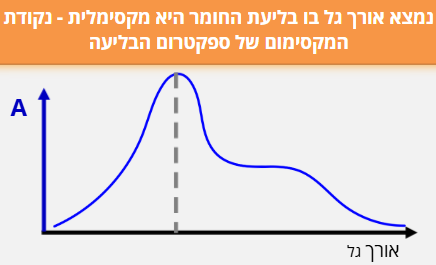
\includegraphics[width=2.95035in,height=1.79322in]{media/media/image6.png}
{}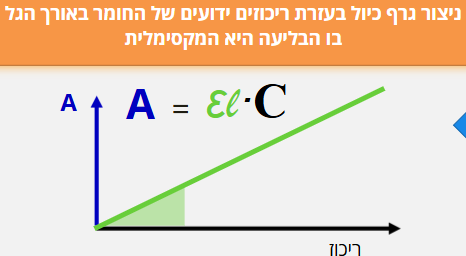
\includegraphics[width=3.26215in,height=1.79209in]{media/media/image7.png}

Figure {7- מציאת ריכוז תמיסת נעלם בשיטות ספקטרוסקופיות - שלב ראשון מציאת
אורך הגל המקסימלי, שלב שני בניית גרף כיול, ושלב שלישי -- מדידת הבליעה של
תמיסת נעלם והסקת הערך המהגרף. כל התמונות מתוך הלומדה ``ספקטרוסקופיה,
מבוא למשוואת ביר למברט'', ד''ר אלינה גולדשטיין לויטין, היחידה לקידום
איכות ההוראה והלמידה באוניברסיטת בן גוריון}

{לאחר שביצענו כיול וקיבלנו גרף המתאר את הקשר בין המשתנה הנמדד למשתנה
הרצוי, נרצה להשתמש בו כדי לחשב ערכים חדשים}. {עם זאת}, \textbf{{לא כל
מצב מחושב באותה דרך}}: {לעיתים יש לנו רק שתי נקודות כיול סמוכות, ולעיתים
סדרת נתונים שלמה שנראית לינארית או מתפזרת סביב קו מגמה. במקרים אחרים
הקשר בין המשתנים כלל אינו לינארי, ולכן נידרש לבצע \textbf{לינאריזציה}}
-- {הגדרה מחדש של המשתנים, או שימוש בגרפים לוגריתמים/חצי לוגריתמים, על
מנת שנוכל לעבד את הגרפים כגרפים ישרים.}

\subsection{\texorpdfstring{{אינטרפולציה
ואקסטרפולציה}}{אינטרפולציה ואקסטרפולציה}}\label{ux5d0ux5d9ux5e0ux5d8ux5e8ux5e4ux5d5ux5dcux5e6ux5d9ux5d4-ux5d5ux5d0ux5e7ux5e1ux5d8ux5e8ux5e4ux5d5ux5dcux5e6ux5d9ux5d4}

{במדידות ניסיוניות אנו אוספים נקודות נתונים המתארות את הקשר בין שני
משתנים, אך לא תמיד נוכל למדוד את כל הערכים האפשריים. לעיתים נרצה להעריך
את ערכו של המשתנה עבור נקודה \textbf{שלא נמדדה ישירות} --} {בין שתי
נקודות ידועות או מחוץ לתחום הנתונים}

\textbf{אינטרפולציה (Interpolation)} --- תהליך הערכת ערכו של משתנה
בנקודה הנמצאת \emph{בתוך} טווח הנתונים הידועים.\\
ההנחה היא שהקשר בין הנקודות בתחום זה נשמר, ולכן ההערכה נחשבת אמינה
יחסית.

\textbf{אקסטרפולציה (Extrapolation)} --- תהליך הערכת ערכו של משתנה
\emph{מחוץ} לטווח הנתונים הידועים.\\
האמינות של האומדן פוחתת ככל שמתרחקים מטווח הנתונים, שכן אין ודאות שהמגמה
שנצפתה בתחום הנמדד נשמרת גם מעבר לו.

{שתי השיטות מבוססות על ההנחה שהקשר שנמצא בין המשתנים נמשך גם בנקודות שלא
נמדדו, אך חשוב לזכור כי באקסטרפולציה גדל הסיכון לשגיאה} -- {אין ודאות
שהמגמה תישמר מעבר לגבולות הנתונים שנמדדו בפועל}. {כדי לבצע חיזויים כאלה
נדרש מודל מתמטי המתאר את הקשר בין המשתנים. מודל זה יכול להיות פשוט --
כמו קו ישר בין שתי נקודות -- או מורכב יותר, כמו עקומה לא ליניארית
המותאמת לנתונים. במקרים אחרים נשתמש בטריקים מתמטיים כמו לינאריזציה או
גרפים לוגיים כדי להציג קשרים מורכבים בצורה פשוטה וברורה}.

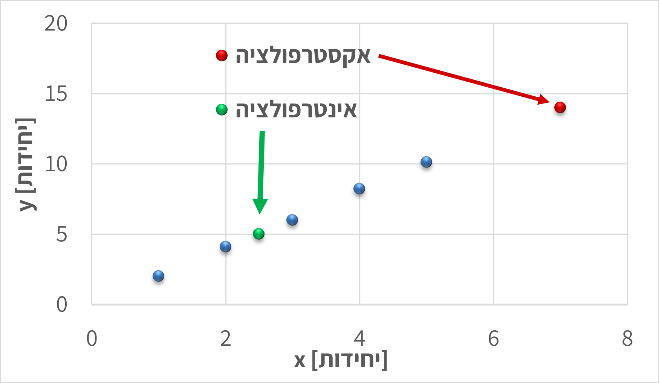
\includegraphics[width=3.20853in,height=1.86736in]{media/media/image9.png}
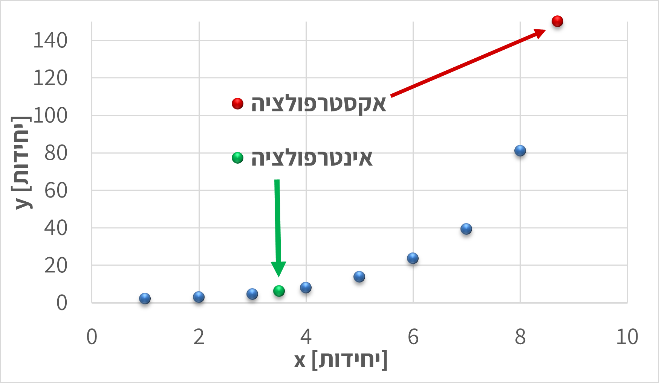
\includegraphics[width=3.17406in,height=1.84745in]{media/media/image10.png}

Figure {8 - בשני הגרפים מוצגות דוגמאות למדידה של ערכים שלא נמדדו ישירות:
הנקודות הכחולות הן הערכים שנמדדו, הנקודות הירוקות מייצגות חיזוי בתוך
תחום המדידות (אינטרפולציה), והנקודות האדומות -- חיזוי מחוץ לתחום המדידות
(אקסטרפולציה), שבו גובר הסיכון לסטות מהמגמה האמיתית}.

\subsection{\texorpdfstring{{אינטרפולציה
מקומית}}{אינטרפולציה מקומית}}\label{ux5d0ux5d9ux5e0ux5d8ux5e8ux5e4ux5d5ux5dcux5e6ux5d9ux5d4-ux5deux5e7ux5d5ux5deux5d9ux5ea}

{כאשר נרצה להעריך את ערכו של משתנה בנקודה שנמצאת בין שתי מדידות ידועות},
{נשתמש ב-\textbf{אינטרפולציה מקומית}} \textbf{(Local Interpolation)}.\\
{הרעיון פשוט: אם שתי נקודות סמוכות מראות מגמה כמעט ישרה, ניתן להניח
שהקשר ביניהן ליניארי בטווח הצר הזה. כך נוכל לחשב את ערך המשתנה המבוקש
לפי קו ישר המחבר בין שתי הנקודות}.

{אם הנקודות הן} \((x_{1},y_{1})\){ו-}\((x_{2},y_{2})\), {ניתן לחשב את}
\(y\) {עבור ערך ביניים של} \(x\){לפי}:

\[y = y_{1} + \frac{x - x_{1}}{x_{2} - x_{1}}(y_{2} - y_{1})\]

{שיטה זו נוחה במיוחד בגרפים ניסיוניים או בטבלאות כיול, שבהם נרצה למצוא
ערך חסר \emph{בתוך} התחום שנמדד}. {עם זאת, יש לזכור כי ההנחה הליניארית
תקפה רק \textbf{בקרבת הנקודות, ובהנחה שהמדידות מדוייקות באופן יחסי.}}
{כאשר המרווחים גדולים, המדידות רועשות, ו/או הנתונים מתנהגים באופן שאינו
לינארי, יש לעבור לשיטות מדויקות יותר כגון התאמת קו או התאמת עקומה}.

Figure {9 - חישוב אינטרפולציה לינארית בין שתי נקודות מדידה סמוכות לצורך
הערכת ערך החסר בתוך טווח הנתונים.}

\subsection{\texorpdfstring{{התאמת קו ישר} (Linear
Fit){.}}{התאמת קו ישר (Linear Fit).}}\label{ux5d4ux5eaux5d0ux5deux5ea-ux5e7ux5d5-ux5d9ux5e9ux5e8-linear-fit.}

{כאשר ברשותנו מספר נקודות מדידה המתארות קשר כמעט ליניארי בין שני משתנים,
נוכל לתאר את הנתונים באמצעות התאמת קו ישר} (Linear Fit){.} {במקרה זה,
אנו לא מסתכלים רק על האזור המסויים בו נמצא הערך שלנו, אלא משתמשים
בנקודות על הגרף על מנת לייצר משוואת קו ישר}.

{המודל המתמטי הוא}:

\[y = ax + b\] {אם נבחר כל שתי נקודות על הקו},
\((x_{1},y_{1})\){ו-}\((x_{2},y_{2})\), {נוכל לחשב את מקדמי המשוואה
לפי}:

\[a = \frac{y_{2} - y_{1}}{x_{2} - x_{1}},b = y_{1} - ax_{1}\] {במקרה זה
משוואת הקו מבוססת על הנקודות אותן בחרנו, לפי ההנחה שאלו שתי הנקודות
שמייצגות את הישר בצורה הטובה ביותר ("לפי העין"). לאחר שמצאנו את משוואת
הקו, נוכל להשתמש בה גם לצורך אינטרפולציה וגם לצורך אקסטרפולציה. עם זאת,
חשוב לזכור כי ככל שנצא רחוק יותר מתחום המדידות}, {האמינות של
האקסטרפולציה פוחתת}. {כאשר הנתונים מצייתים באופן הדוק לקו ישר, ניתן
להתאים את הקו ``בעין'' או על סמך שתי נקודות בלבד. אך כאשר קיים פיזור או
רעש מדידה, יש להיעזר בכלים סטטיסטיים מדויקים יותר.}

Figure {10 הגרף מציג שתי התאמות לינאריות לסט נתונים זהה, כאשר כל אחת
מבוססת על זוג נקודות שונה. השוואת הקווים מדגימה כיצד בחירת נקודות שונות
משפיעה על שיפוע ונקודת החיתוך של המשוואה}

\subsection{\texorpdfstring{{רגרסיה לינארית} (Linear
Regression)}{רגרסיה לינארית (Linear Regression)}}\label{ux5e8ux5d2ux5e8ux5e1ux5d9ux5d4-ux5dcux5d9ux5e0ux5d0ux5e8ux5d9ux5ea-linear-regression}

{במדידות אמיתיות כמעט תמיד קיימות שגיאות מדידה ורעש אקראי. לכן, גם אם
הקשר בין המשתנים ליניארי באופן עקרוני, הנקודות בפועל אינן נופלות בדיוק
על קו אחד אלא מפוזרות סביבו}. {במצב כזה, לא ניתן לבחור שתי נקודות ולבנות
מהן קו מייצג -- יש צורך בשיטה שתמצא את הקו ``הכי מתאים}'' {לכל הנתונים
יחד}. {שיטה זו נקראת רגרסיה ליניארית}, {והיא מבוססת על עיקרון ה-}Least
Squares{, "שיטת הריבועים הפחותים".}\\
{לפי עיקרון זה, נבחר את השיפוע} \(a\) {והחיתוך} \(b\) {של הקו}
\(y = ax + b\) {כך שסכום הריבועים של ההפרשים בין הערכים הנמדדים}
\(y_{i}\) {לערכים החזויים לפי הקו יהיה הקטן ביותר}:

\[\text{minimal\:\,\:\,}\sum_{i}^{}{(y_{i} - (ax_{i} + b))^{2}}\]
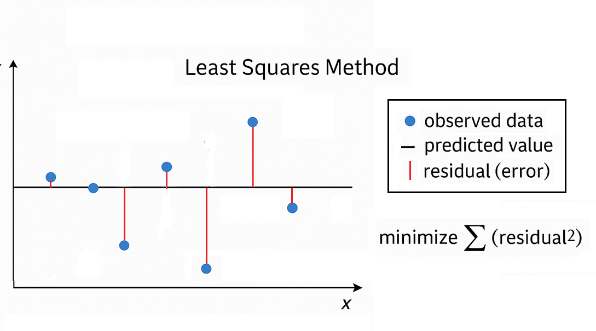
\includegraphics[width=2.69075in,height=1.27926in]{media/media/image13.png}

{כלומר, הקו שנבחר הוא זה שמייצג בצורה הטובה ביותר את כלל הנתונים, גם אם
כל נקודה בודדת סוטה ממנו מעט}.

{רגרסיה ליניארית אינה רק דרך ציור מדויקת יותר של קו; היא גם מספקת
\textbf{מדדים כמותיים} לאיכות ההתאמה, כמו מקדם הקורלציה} \(R^{2}\),
{המעיד עד כמה הקו מתאר את הנתונים היטב}.

{במעבדות ובתעשייה, רגרסיה ליניארית משמשת לעיתים קרובות ליצירת
\textbf{עקומות כיול אמינות}} -- {למשל, במכשירי ספקטרופוטומטר, שבהם נבנה
קו כיול על סמך מדידות רועשות ומחשבים את ריכוז הדגימה הלא ידועה לפי
משוואת הקו שהתקבלה}.

Figure {11 - הנקודות המייצגות נתונים ניסיוניים, והקו מציג את קו הרגרסיה
שנקבע לפי שיטת הריבועים הפחותים.}

\subsection{\texorpdfstring{{התאמת עקומה לא ליניארית} (Nonlinear Curve
Fitting)}{התאמת עקומה לא ליניארית (Nonlinear Curve Fitting)}}\label{ux5d4ux5eaux5d0ux5deux5ea-ux5e2ux5e7ux5d5ux5deux5d4-ux5dcux5d0-ux5dcux5d9ux5e0ux5d9ux5d0ux5e8ux5d9ux5ea-nonlinear-curve-fitting}

{לא כל קשר בין משתנים הוא ליניארי. במקרים רבים -- במיוחד בתהליכים
כימיים, ביולוגיים או פיזיקליים -- הנתונים מראים \textbf{עקומה ברורה}}:
{הקצב משתנה עם הזמן, הבליעה מתקרבת לערך רוויה, או הלחץ תלוי בריבוע
הטמפרטורה. במצבים כאלה, קו ישר כבר אינו מתאים, ונדרש לבצע \textbf{התאמת
עקומה לא ליניארית}}.

{במקום להשתמש במשוואה מהצורה} \(y = ax + b\), {נבחר פונקציה שתואמת את
האופי של הנתונים, למשל}:

\[y = ae^{bx},y = ax^{b},y = a(x - x_{0})^{2} + c\]

{נחשב את הפרמטרים} \(a,b,c\){כך שהעקומה תתאים בצורה הטובה ביותר למדידות
-- לעיתים בעזרת חישוב ממוחשב (למשל בשיטת הריבועים המינימליים
הלא-ליניארית)}. {לעיתים נבחר את הצורה של הפונקציה לפי ידע פיזיקלי מוקדם
(למשל תגובה אקספוננציאלית או קצב תלוי חזקתית), ובמקרים אחרים פשוט נבחן
איזו פונקציה מתאימה טוב יותר לנתונים}.

Figure 12 -- {הגרף מציג נתונים המתואמים לעקומה מהצורה} {\(y = 2x^{3}\)}
{, כדוגמה למקרה שבו הקשר בין המשתנים אינו ליניארי.}

עם זאת, התאמות לא־ליניאריות קשות יותר להערכה אינטואיטיבית: בעקומה מורכבת
קשה לעין האנושית להבחין אם ההתאמה ``מדויקת'' או לא, במיוחד כשיש כמה
פרמטרים חופשיים. לכן חשוב להיעזר גם בידע הפיזיקלי על התהליך וגם במדדים
מספריים (כמו \(R^{2}\) או סטיות התקן של הפרמטרים) כדי לוודא שההתאמה
סבירה ולא רק מתמטית. לבסוף, ככל שמספר הפרמטרים גדל, כך גם הסיכון ל־התאמת
יתר (overfitting) --- מצב שבו הפונקציה ``מתאימה'' את עצמה לכל נקודה אך
מאבדת משמעות פיזיקלית.

\href{simulations/leastsquares.html}{סימולציה: המחשת שיטת הריבועים
המינימליים}

\subsection{\texorpdfstring{\textbf{{לינאריזציה}}
(Linearization)}{לינאריזציה (Linearization)}}\label{ux5dcux5d9ux5e0ux5d0ux5e8ux5d9ux5d6ux5e6ux5d9ux5d4-linearization}

{במקרים רבים נעדיף להמיר קשר לא ליניארי לקשר \textbf{ליניארי}}, {כדי
להקל על ניתוח הנתונים או על התאמת קו ישר. פעולה זו נקראת
\textbf{לינאריזציה}} -- {הפיכת המשוואה לצורה ישרה על-ידי שינוי המשתנים
או הצירים}.

Figure 13 -- {לינאריזציה עבור הגרף מתמונה 11. לאחר החלפת המשתנה} {x}
{במשתנה} {\(z = x^{3}\)} {, התקבל גרף ליניארי.}

הרעיון פשוט: אם ניתן לכתוב את המשוואה כך שתתקבל הצגה מהצורה

\[
f(x) = a\,g(x) + b
\]

אז גרף של ( f(x) ) לעומת ( g(x) ) יניב \textbf{קו ישר}, שממנו ניתן לחשב
את השיפוע ( a ) והחיתוך ( b ).

\[
y = 3x^{3}
\]

נגדיר משתנה חדש ( u = x\^{}\{3\} ).\\
גרף של ( y ) מול ( u ) הוא קו ישר עם שיפוע ( 3 ) וחיתוך ( 0 ).

דוגמה נוספת:

\[
y = a e^{bx}
\]

נחיל לוג טבעי על שני צידי המשוואה:

\([\ln y = \ln a + b x]\)

גרף של \(\ln y\) מול \(x\) הוא קו ישר:\\
השיפוע הוא \(b\), והחיתוך עם הציר הוא \(\ln a\).

{השימוש בלינאריזציה מקל מאוד על זיהוי מגמות, על חישוב פרמטרים, ועל הערכת
איכות ההתאמה בעין -- מאחר שקל לנו יותר לזהות ``ישרות'' של קו מאשר
עקמומיות של עקומה}.\\
{עם זאת, יש לזכור שלינאריזציה משנה את יחידות הצירים ואת משמעות המשתנים,
ולכן יש \textbf{להחזיר את התוצאה למשתנים המקוריים} בסיום הניתוח}.

\begin{tcolorbox}[enhanced jigsaw, colback=white, arc=.35mm, coltitle=black, breakable, toptitle=1mm, leftrule=.75mm, colbacktitle=quarto-callout-tip-color!10!white, opacitybacktitle=0.6, bottomtitle=1mm, titlerule=0mm, opacityback=0, colframe=quarto-callout-tip-color-frame, title=\textcolor{quarto-callout-tip-color}{\faLightbulb}\hspace{0.5em}{טיפ: דפי עבודה אינטראקטיביים לריבועים המינימליים}, rightrule=.15mm, bottomrule=.15mm, toprule=.15mm, left=2mm]

רוצים לתרגל צעד-אחר-צעד את חישוב קו הרגרסיה אחרי לינאריזציה של מודל
לא-ליניארי?\\
הקישורים הבאים מובילים לדפי עבודה אינטראקטיביים (הסימולציה תיפתח בעמוד
חדש):

\begin{itemize}
\tightlist
\item
  \href{simulations/LeastSquaresCalc.html}{דף עבודה 1 -- חישוב קו
  הרגרסיה צעד-אחר-צעד}
\item
  \href{simulations/LeastSquaresCalc2.html}{דף עבודה 2 -- הדגמה, מציאת
  הקשר בין הזמן לכמות חלבון}
\end{itemize}

מומלץ לפתוח את דפי העבודה בלשונית נפרדת, ולחזור לפרק תוך כדי פתרון.

\end{tcolorbox}

\subsection{\texorpdfstring{{שימוש בגרפים לוגיים
וסמילוגיים}}{שימוש בגרפים לוגיים וסמילוגיים}}\label{ux5e9ux5d9ux5deux5d5ux5e9-ux5d1ux5d2ux5e8ux5e4ux5d9ux5dd-ux5dcux5d5ux5d2ux5d9ux5d9ux5dd-ux5d5ux5e1ux5deux5d9ux5dcux5d5ux5d2ux5d9ux5d9ux5dd}

{לפני עידן המחשבים, אחת הדרכים הנפוצות לנתח נתונים ניסיוניים הייתה שימוש
בגרפים לוגיים} (Log-- {}Log) {ו-סמילוגיים} (Semi--Log){. גרפים אלה שימשו
להמחשה גרפית של קשרים מתמטיים לא ליניאריים -- בעיקר קשרים אקספוננציאליים
ו-חזקתיים --} {והיו כלי בסיסי בעבודתו של כל מהנדס או חוקר}. {}

Figure {14} {- דפים לוגריתמים וסמי לוגריתמים. שימוש בגרפים מסוג זה מאפשר
להציג קשרים אקספוננציאליים וחזקתיים כקווים ישרים, ולזהות בקלות את טיב
הקשר בין המשתנים}.

Figure {15השוואה בין גרף ליניארי, סמי-לוגריתמי ולוגריתמי-לוגריתמי.}

\begin{longtable}[]{@{}
  >{\centering\arraybackslash}p{(\linewidth - 6\tabcolsep) * \real{0.2500}}
  >{\centering\arraybackslash}p{(\linewidth - 6\tabcolsep) * \real{0.2500}}
  >{\centering\arraybackslash}p{(\linewidth - 6\tabcolsep) * \real{0.2500}}
  >{\centering\arraybackslash}p{(\linewidth - 6\tabcolsep) * \real{0.2500}}@{}}
\toprule\noalign{}
\begin{minipage}[b]{\linewidth}\centering
\textbf{סוג גרף}
\end{minipage} & \begin{minipage}[b]{\linewidth}\centering
\textbf{ליניארי}
\end{minipage} & \begin{minipage}[b]{\linewidth}\centering
\textbf{סמי־לוגריתמי}
\end{minipage} & \begin{minipage}[b]{\linewidth}\centering
\textbf{לוג־לוגריתמי}
\end{minipage} \\
\midrule\noalign{}
\endhead
\bottomrule\noalign{}
\endlastfoot
\textbf{צירי הסקאלה} & שני הצירים ליניאריים & ציר אחד (בדרך כלל \(y\))
לוגריתמי, והשני ליניארי & שני הצירים לוגריתמיים \\
\textbf{סוג הקשר} & קשר ישר & קשר אקספוננציאלי & קשר חזקתי \\
\textbf{צורת המשוואה} & \(y = a + bx\) & \(y = a e^{bx}\) &
\(y = a x^{b}\) \\
\textbf{פירוש השיפוע (\(m\))} & קצב שינוי קבוע של \(y\) ביחס ל־\(x\) &
קצב הגידול או הדעיכה האקספוננציאלי & המעריך (\(b\)) בקשר החזקתי \\
\textbf{חישוב השיפוע בפועל} & \(m = \dfrac{\Delta y}{\Delta x}\) &
\(b = \dfrac{\ln(y_2) - \ln(y_1)}{x_2 - x_1}\) &
\(b = \dfrac{\log(y_2) - \log(y_1)}{\log(x_2) - \log(x_1)}\) \\
\textbf{משמעות פיזיקלית} & השיפוע הוא השינוי המוחלט (כמו מהירות, קצב
זרימה וכו׳) & מציין שיעור שינוי יחסי קבוע (למשל קצב דעיכה רדיואקטיבית) &
מתאר יחס קנה־מידה --- כיצד \(y\) משתנה כאשר \(x\) מוכפל פי ערך קבוע \\
\end{longtable}

{כיום, בעידן התוכנות והחישובים הדיגיטליים, כמעט ואין צורך לצייר גרפים
לוגריתמיים באופן ידני}.\\
{עם זאת}, {הבנה של הצגה לוגית חשובה מאוד -- היא מאפשרת לנו להעריך בצורה
נכונה שינויים לוגריתמיים או אקספוננציאליים (למשל גידול מעריכי או דעיכה
מהירה), ולפרש נכונה גרפים מדעיים שבהם קני מידה כאלה עדיין נפוצים}.

\textbf{בטבלת הכיול הבאה נמדדה בליעת אור (y, ביחידות a.u.) עבור ריכוזים
שונים של חומר (x, ביחידות mol/L):}

\begin{longtable}[]{@{}cccccc@{}}
\toprule\noalign{}
x (mol/L) & \textbf{0.10} & \textbf{0.20} & \textbf{0.30} &
\textbf{0.40} & \textbf{0.50} \\
\midrule\noalign{}
\endhead
\bottomrule\noalign{}
\endlastfoot
y (a.u.) & 0.48 & 0.96 & 1.45 & 1.94 & 2.44 \\
יחידות שרירותיות & & & & & \\
\end{longtable}

\begin{enumerate}
\def\labelenumi{\arabic{enumi}.}
\tightlist
\item
  השתמשו באינטרפולציה מקומית כדי להעריך את ערך הבליעה עבור
  \textbf{y=1.70a.u.}\\
\item
  מצאו את משוואת הקו המתארת את הנתונים, בהנחה שהקשר ליניארי.\\
\item
  השתמשו במשוואה שמצאתם כדי למצוא את הריכוז עבור \textbf{y=2.85a.u.}\\
\item
  אילו היה מספר רב של נקודות מדידה, באיזו מן השיטות המוזכרות בפרק היה
  כדאי להשתמש?
\end{enumerate}

\subsection{סט תרגילים: בחירת שיטת הערכה מנתונים
גרפיים}\label{ux5e1ux5d8-ux5eaux5e8ux5d2ux5d9ux5dcux5d9ux5dd-ux5d1ux5d7ux5d9ux5e8ux5ea-ux5e9ux5d9ux5d8ux5ea-ux5d4ux5e2ux5e8ux5dbux5d4-ux5deux5e0ux5eaux5d5ux5e0ux5d9ux5dd-ux5d2ux5e8ux5e4ux5d9ux5d9ux5dd}

כאשר אנו רוצים להעריך נתונים, אנחנו ננסה לעשות את זה מצד אחד מדוייק ומצד
שני מהר. לכן ננסה לחפש את השיטה שתתן לנו את התוצאה הכי קרובה במינימום
מאמץ. נסו לענות על השאלות הבאות ולנמק מדוע בחרתם כל שיטה. יכולות להיות
תשובות רבות, מה שחשוב הוא הנימוק. התשובות פה ממחישות נימוקים אפשריים
לבחירה מסויימת.

\begin{figure}

\centering{

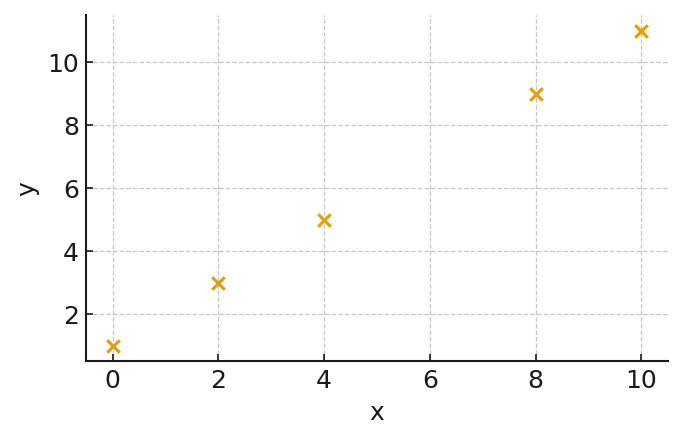
\includegraphics[width=0.6\linewidth,height=\textheight,keepaspectratio]{images/ex1.png}

}

\caption{\label{fig-ex1}גרף לשאלה 1}

\end{figure}%

בגרף מוצגים נתונים של (y) כפונקציה של (x). הנקודות כמעט מסודרות על קו
ישר. אין ברשותינו מחשב זמין, אלא רק מחשבון פשוט יחסית.

נרצה להעריך את הערך של (y) עבור ערך ביניים של (x).

באיזו שיטה כדאי להשתמש?

\begin{tcolorbox}[enhanced jigsaw, colback=white, arc=.35mm, coltitle=black, breakable, toptitle=1mm, leftrule=.75mm, colbacktitle=quarto-callout-note-color!10!white, opacitybacktitle=0.6, bottomtitle=1mm, titlerule=0mm, opacityback=0, colframe=quarto-callout-note-color-frame, title=\textcolor{quarto-callout-note-color}{\faInfo}\hspace{0.5em}{פתרון}, rightrule=.15mm, bottomrule=.15mm, toprule=.15mm, left=2mm]

יש לנו נקודות שיוצרות קו שנראה ישר יחסית כשהנקודה נמצאת בתוך הטווח, אבל
רחוקה מנקודות אחרות, ולכן כדאי להשתמש בשיטה של התאמה פשוטה של קו ישר.

\end{tcolorbox}

\begin{figure}

\centering{

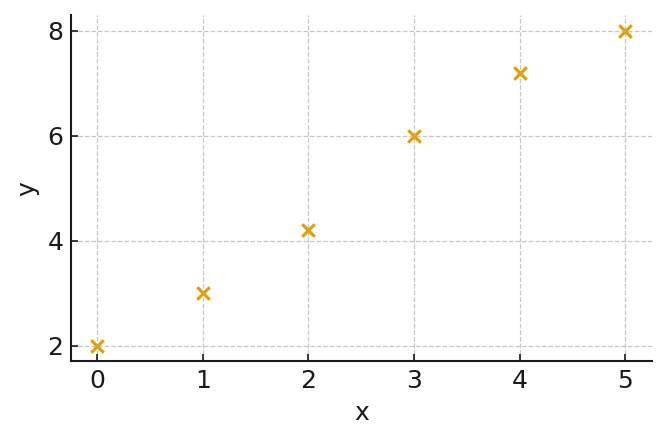
\includegraphics[width=0.6\linewidth,height=\textheight,keepaspectratio]{images/ex2.png}

}

\caption{\label{fig-ex2}גרף לשאלה 2}

\end{figure}%

בגרף מוצגים ערכי (y) כפונקציה של הזמן (t) בין (t=0) לבין (t=5). נרצה
להעריך את ערך (y) בזמן (t=8), מחוץ לטווח המדידה.

איזו שיטה מתאימה ביותר כדי להעריך את (y) בזמן (t=8)?

\begin{tcolorbox}[enhanced jigsaw, colback=white, arc=.35mm, coltitle=black, breakable, toptitle=1mm, leftrule=.75mm, colbacktitle=quarto-callout-note-color!10!white, opacitybacktitle=0.6, bottomtitle=1mm, titlerule=0mm, opacityback=0, colframe=quarto-callout-note-color-frame, title=\textcolor{quarto-callout-note-color}{\faInfo}\hspace{0.5em}{פתרון}, rightrule=.15mm, bottomrule=.15mm, toprule=.15mm, left=2mm]

הגרף נראה יחסית לינארי, אבל עם סטיות למעלה ולמטה, כמו כן, באקסטרפולציה
השגיאה גדלה ולכן נרצה ישר מדוייק ככל האפשר, ולכן נעשה רגרסיה לינארית

\end{tcolorbox}

\begin{figure}

\centering{

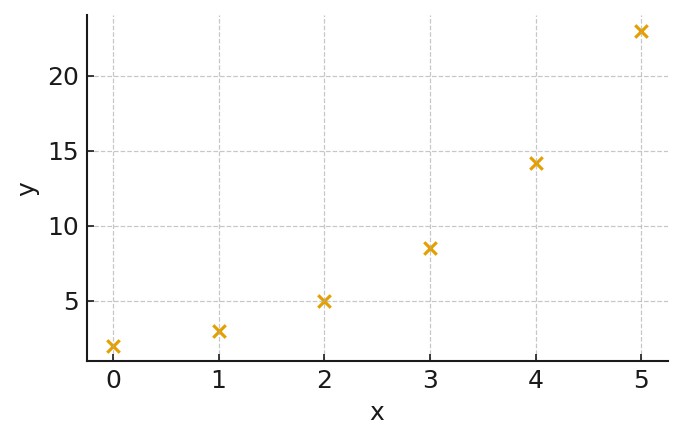
\includegraphics[width=0.6\linewidth,height=\textheight,keepaspectratio]{images/ex4.png}

}

\caption{\label{fig-ex4}גרף לשאלה 4}

\end{figure}%

בגרף מוצגת גדילה שנראית אקספוננציאלית של (y) כפונקציה של הזמן (t). הקשר
מתואר על ידי מודל פיסיקלי מהצורה (y = Ce\^{}\{kt\}).

כיצד נבנה את המשוואה ונמצא את הקבועים המתאימים למודל?

\begin{tcolorbox}[enhanced jigsaw, colback=white, arc=.35mm, coltitle=black, breakable, toptitle=1mm, leftrule=.75mm, colbacktitle=quarto-callout-note-color!10!white, opacitybacktitle=0.6, bottomtitle=1mm, titlerule=0mm, opacityback=0, colframe=quarto-callout-note-color-frame, title=\textcolor{quarto-callout-note-color}{\faInfo}\hspace{0.5em}{פתרון}, rightrule=.15mm, bottomrule=.15mm, toprule=.15mm, left=2mm]

עבור מודל \(\(y = Ce^{kt}\)\) נפעיל ln על שני האגפים, ונקבל קשר לינארי
בין \(\(\ln y\)\) לבין t, ואז נעשה רגרסיה לינארית על הנתונים. מאחר
ומדובר במציאת קבועים לתיאור מערכת פיסיקלית נבחר בשיטה הכי מדוייקת שיש
לנו. ברמה העקרונית ניתן להשתמש גם בשיטת הריבועים המינימלים עבור רגרסיה
שאינה לינארית, אך במקרה זה החישוב הוא משמעותית יותר מסובך ולא ניתן לפתור
אותו באופן ישיר אלא רק בצורה נומרית.

\end{tcolorbox}

\begin{figure}

\centering{

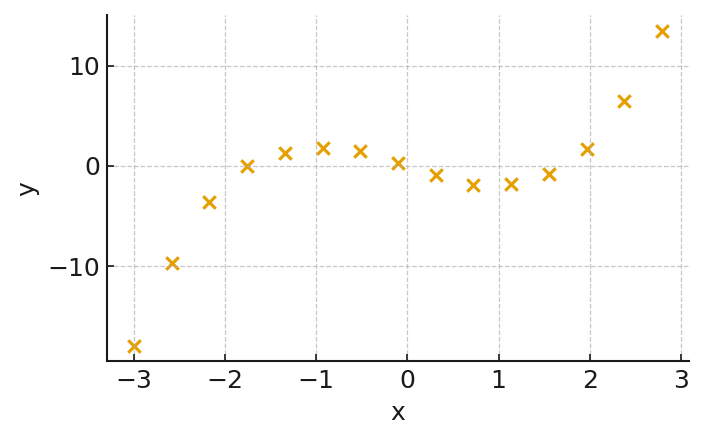
\includegraphics[width=0.6\linewidth,height=\textheight,keepaspectratio]{images/ex5.png}

}

\caption{\label{fig-ex5}גרף לשאלה 5}

\end{figure}%

בגרף מוצגת פונקציה כללית של (y) מול (x). נרצה להעריך את ערך (y)
ב-(x=1.8),אך אין לנו מודל פיסיקלי המתאר את המערכת איזו שיטה עדיפה?

\begin{tcolorbox}[enhanced jigsaw, colback=white, arc=.35mm, coltitle=black, breakable, toptitle=1mm, leftrule=.75mm, colbacktitle=quarto-callout-note-color!10!white, opacitybacktitle=0.6, bottomtitle=1mm, titlerule=0mm, opacityback=0, colframe=quarto-callout-note-color-frame, title=\textcolor{quarto-callout-note-color}{\faInfo}\hspace{0.5em}{פתרון}, rightrule=.15mm, bottomrule=.15mm, toprule=.15mm, left=2mm]

כאן מעניינת אותנו התנהגות מקומית באזור קטן, ולא מודל גלובלי לכל התחום.
הנקודות קרובות יחסית, ורואים מגמה עקבית ולא רועשת, כך שסביר מאוד
שהפונקציה עצמה פועלת באופן מאוד קרוב לנתונים, וכי המשתנים בין כל שתי
נקודות סמוכות מתנהגים כקו ישר. לכן נבחר באינטרפולציה מקומית

\end{tcolorbox}

\subsection{\texorpdfstring{{סיכום}}{סיכום}}\label{ux5e1ux5d9ux5dbux5d5ux5dd-2}

בעבודה הנדסית וניסויית אנו כמעט תמיד נדרשים להסיק מסקנות מתוך מדידות
חלקיות.\\
האתגר הוא לייצג את הנתונים בדרך שתאפשר לנבא ערכים חדשים ולבדוק אם הם
סבירים מבחינה פיזיקלית.\\
לשם כך עומדים לרשותנו כלים ברמות שונות של מורכבות:

\begin{itemize}
\tightlist
\item
  \textbf{אינטרפולציה מקומית} מאפשרת להעריך ערכים \emph{בין} שתי נקודות
  סמוכות.\\
\item
  \textbf{התאמת קו ישר} יוצרת מודל פשוט שמתאר את המגמה הכללית של נתונים
  שנראים ליניאריים באופן יחסי.\\
\item
  \textbf{רגרסיה ליניארית} מחשבת קו מייצג סטטיסטי כאשר קיימות סטיות ורעש
  מדידה.\\
\item
  \textbf{התאמת עקומה לא־ליניארית} מרחיבה את השיטה למקרים שבהם הקשר בין
  המשתנים מתואר בעזרת פונקציה מורכבת יותר.
\item
  \textbf{ליניאריזציה וגרפים לוגריתמיים} מאפשרים להפוך קשרים
  לא־ליניאריים לייצוגים ישרים שקל לנתח בעין ובחישוב.
\end{itemize}

בין אם מדובר בקו פשוט או בעקומה מורכבת, המטרה המשותפת היא אחת -\\
למצוא תיאור מתמטי אמין של הנתונים ולבחון עד כמה הוא מייצג את המציאות.\\
גם בעידן שבו תוכנות מבצעות עבורנו את כל ההתאמות בלחיצת כפתור, חשוב להבין
את העקרונות שמאחורי השיטות:\\
רק כך נוכל להעריך את אמינות התוצאות, לזהות מתי חיזוי הוא סביר ומתי מדובר
באקסטרפולציה מסוכנת,\\
ולשלב בין ניתוח מתמטי לבין שיקול הנדסי ופיזיקלי נכון.

\bookmarksetup{startatroot}

\chapter{\texorpdfstring{{תהליכים ומשתני
תהליך}}{תהליכים ומשתני תהליך}}\label{ux5eaux5d4ux5dcux5d9ux5dbux5d9ux5dd-ux5d5ux5deux5e9ux5eaux5e0ux5d9-ux5eaux5d4ux5dcux5d9ux5da}

\section{\texorpdfstring{{מה נלמד בפרק
הזה}?}{מה נלמד בפרק הזה?}}\label{ux5deux5d4-ux5e0ux5dcux5deux5d3-ux5d1ux5e4ux5e8ux5e7-ux5d4ux5d6ux5d4-1}

\begin{itemize}
\item
  {{להגדיר ולהסביר} את המושגים הבסיסיים של צפיפות, משקל סגולי, יחידות
  מוליות} {(}mole gram-mole, pound-mole{), וגדלי טמפרטורה ולחץ}.
\item
  {{להמחיש ולזהות} משתנים בתרשים תהליך -- זרמים, משתני מצב והרכב --
  ולתאר את תפקידם בתהליך הנדסי}.
\item
  {{להבדיל ולהשוות} בין סוגי לחצים (מוחלט, נמדד ואטמוספרי), ולנתח מצבים
  בהם הלחץ נמדד בעזרת מנומטר או עמוד נוזל}.
\item
  {{לבצע ולנמק} חישובים המקשרים בין מסה, נפח ומולים, בהתבסס על צפיפות
  ומשקל מולקולרי}.
\item
  {{להמיר ולפרש} הרכב תערובת בין שברי מסה לשברי מולים, ולחשב משקל
  מולקולרי ממוצע של תערובת מרובת רכיבים}.
\item
  {{להמיר ולהעריך} יחידות טמפרטורה בין קלווין, צלזיוס, פרנהייט וראנקין,
  ולהבין את משמעות הבחירה ביחידת מידה בתיאור תהליך פיזיקלי או
  ביוטכנולוגי}.
\end{itemize}

\section{\texorpdfstring{{מהו תהליך
הנדסי?}}{מהו תהליך הנדסי?}}\label{ux5deux5d4ux5d5-ux5eaux5d4ux5dcux5d9ux5da-ux5d4ux5e0ux5d3ux5e1ux5d9}

{תהליך הוא רצף של פעולות פיזיקליות או כימיות שבמהלכן חומרי גלם עוברים
שינוי} {בהרכבם, בצורתם או באנרגיה שלהם.}

{לעבודתם של מהנדסי ומהנדסות התהליך שלושה היבטים: תכנון, תפעול
ואופטימיזציה של תהליכים במפעלי הייצור השונים, כך שהתהליכים יהיו יציבים,
בטוחים, רווחיים ויעילים לאורך זמן.}

\textbf{{תכנון התהליך} (Process Design)} -- {הגדרה של יחידות הפעולה,
תנאי ההפעלה והציוד הדרוש כך שהתהליך יעמוד במטרות הייצור ובדרישות
הבטיחות}.

\textbf{{תפעול התהליך} (Process Operation)} -- {פיקוח יומיומי על תהליך
קיים, ניטור נתונים בזמן אמת, וזיהוי חריגות או תקלות בתפקוד המערכת}.

\textbf{{אופטימיזציה של התהליך} (Process Optimization)} -- {ניתוח
ביצועים וחיפוש מתמיד אחר דרכים לשפר יעילות, להפחית צריכת אנרגיה ולהגדיל
תפוקה}.

{שלושת השלבים הללו משקפים את עיקר העשייה של מהנדס ומהנדסת תהליך: לא רק
להבין מה קורה במערכת, אלא גם \textbf{לדעת לשלוט בה ולכוון אותה}}.

{כל תהליך בנוי מיחידות פעולה} (Unit Operations)

{יחידות פעולה}- (Unit Operations) {רכיבים נפרדים שכל אחד מהם מבצע שינוי
מסוים בחומר}:

Figure {16- תיאור כללי של תהליך בדיאגרמת בלוקים}

{יש סוגים רבים של יחידות פעולה, אך הבסיסיות ביותר, בהן נשתמש בספר זה, הן
--}

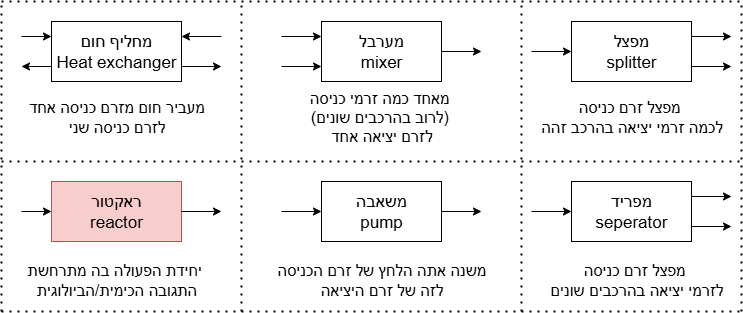
\includegraphics[width=6.5in,height=2.7375in]{media/media/image20.png}
Figure {17 - יחידות פעולה בסיסיות בתהליך הכימי/ביולוגי}

\subsection{\texorpdfstring{{דיאגרמות לתכנון
תהליך}}{דיאגרמות לתכנון תהליך}}\label{ux5d3ux5d9ux5d0ux5d2ux5e8ux5deux5d5ux5ea-ux5dcux5eaux5dbux5e0ux5d5ux5df-ux5eaux5d4ux5dcux5d9ux5da}

{מהנדסים משתמשים בתרשימים שונים כדי לתאר תהליכים -- כל תרשים מתאים לרמת
פירוט אחרת של התכנון}.

\begin{enumerate}
\def\labelenumi{\arabic{enumi}.}
\item
  \textbf{Block Flow Diagram (BFD)}
\end{enumerate}

תרשים כללי ופשוט המתאר את מבנה התהליך ברמת המאקרו. הוא מציג את שלבי
העיבוד העיקריים ואת כיווני זרימת החומר ביניהם, ללא פירוט של ציוד, נתונים
תרמודינמיים או יחידות מדידה. תרשימי BFD משמשים להבנת עקרון הפעולה של
התהליך ולתקשורת ראשונית בין צוותים הנדסיים בשלב התכנון המוקדם.

Figure {18} {-} Block flow process diagram for the production of benzene
(Turton et al., 2012)

\begin{enumerate}
\def\labelenumi{\arabic{enumi}.}
\setcounter{enumi}{1}
\item
  \textbf{Process Flow Diagram (PFD)}
\end{enumerate}

תרשים המשמש לתכנון הנדסי מפורט של תהליך. הוא כולל את כל יחידות הפעולה
העיקריות, קווים לכל זרמי החומר והאנרגיה, ונתוני פעולה בסיסיים כגון
טמפרטורה (T), לחץ (P) וספיקות. לעיתים מוצג בו גם ציוד עזר חשוב. תרשימי
PFD משמשים לביצוע חישובי מאזן חומר ואנרגיה ולשלבי התכנון הראשוניים של
תהליך תעשייתי.

Figure {19-} Process Flow Diagram Detailing the Nitric Acid Process
(Towler and Sinnott, 2013)

\textbf{Piping and Instrumentation Diagram (P\&ID)}

התרשים המפורט ביותר בתכנון התהליך. הוא כולל את כל קווי הצנרת, השסתומים,
החיישנים, מכשירי המדידה, יחידות הבקרה והאזעקות. תרשימי P\&ID משמשים
מהנדסי מכשור, בקרה ותפעול בשלבי הבנייה, ההפעלה והתחזוקה של מתקנים
תעשייתיים.

Figure {20 - תזרים צנרת ומכשור.} Copyright © 2025 Edrawsoft

{\ul{כיצד נצייר תהליך?}}

כדי לנתח תהליך, נייצג אותו באופן סכמטי כתרשים בלוקים (Block Flow Diagram
- BFD). כל בלוק מייצג יחידת פעולה אחת, וחצים מייצגים את זרמי החומר או
האנרגיה הנכנסים והיוצאים מן הבלוקים. ליד כל חץ נציין את שם הזרם ואת
המשתנים הפיזיקליים החשובים: טמפרטורה (T), לחץ (P), ספיקת מסה (ṁ), והרכב
(xᵢ). לעיתים מסמנים גם מסגרת גבולות מערכת (System Boundary), המגדירה מה
נכלל בתהליך ומה לא. כך נוצר ייצוג גרפי של תהליך מורכב, שממנו ניתן בהמשך
לגזור את משוואות מאזן החומר והאנרגיה.

{תהליך תסיסה} (Fermentation Process) {כדי להמחיש את רעיון התרשים, נבחן
תהליך פשוט של ייצור בירה}. {בתהליך זה מוזרמים שני חומרים למיכל תסיסה}
(Fermentation Reactor):{\hfill\break
- תמיסת סוכר} (Substrate Feed) {מהווה את מקור האנרגיה
לשמרים}.{\hfill\break
- תמיסת שמרים} (Cell Suspension) {מכילה תאים חיים המבצעים את התגובה
הביולוגית}. {בתוך המיכל מתרחשת תגובה ביוכימית}: {השמרים ממירים את
הסוכרים ל-אתנול (מוצר רצוי) ו-פחמן דו-חמצני (תוצר לוואי) מהמיכל יוצא זרם
אחד ובו תערובת של מים, אתנול ותאים מתים}. {וזרם נוסף של פחמן דו חמצני
במצב גזי} {תרשים התהליך ייראה כך}:
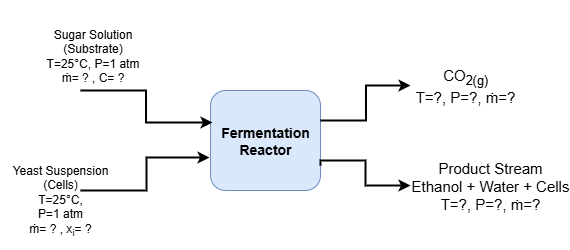
\includegraphics[width=5.9375in,height=2.60417in]{media/media/image24.png}
Figure {21 - תרשים בלוקים - מערכת תסיסה}

\section{\texorpdfstring{{משתני
תהליך}}{משתני תהליך}}\label{ux5deux5e9ux5eaux5e0ux5d9-ux5eaux5d4ux5dcux5d9ux5da}

{אחר שזיהינו את שלבי התהליך ואת יחידות הפעולה המרכיבות אותו, נוכל להתחיל
לבחון אותו לעומק. כל אחת מהיחידות בתהליך -- בין אם מדובר במיכל ערבוב,
במחליף חום או במגדל ספיגה -- מאופיינת על-ידי משתני תהליך} (process
variables){.}

\textbf{{משתני תהליך} (Process Variables)} {הם גדלים פיזיקליים או כימיים
הנמדדים או נשלטים במהלך פעולה של מערכת תהליכית, ומשמשים לתיאור מצבה בזמן
נתון.}

{משתנים אלה כוללים גדלים כמו טמפרטורה, לחץ, ספיקה, ריכוז והרכב כימי},
{והם אלה שמאפשרים לנו לכמת את מה שקורה בכל שלב של התהליך. במילים אחרות,
אם תרשים הבלוקים מציג לנו את ``מה קורה'' בתהליך, משתני התהליך הם
\textbf{השפה הכמותית} שבאמצעותה מהנדסים ומהנדסות מתארים מה מתרחש בתוך כל
יחידת פעולה, וכיצד שינוי באחד מהם משפיע על שאר מרכיבי המערכת}.

\textbf{דוגמאות למשתני תהליך}

\begin{longtable}[]{@{}ccc@{}}
\toprule\noalign{}
\textbf{סוג המשתנה} & \textbf{דוגמאות} & \textbf{מה הוא מתאר} \\
\midrule\noalign{}
\endhead
\bottomrule\noalign{}
\endlastfoot
תרמודינמי & טמפרטורה (T), לחץ (P) & מצבי אנרגיה והתנהגות חומרים \\
זרימה & ספיקה מסה / נפח & כמה חומר עובר ביחידת זמן \\
הרכב & ריכוז, אחוז מסה, שבר מולרי & תכולת חומרים בתערובת \\
\end{longtable}

\section{\texorpdfstring{{מסה
ונפח}}{מסה ונפח}}\label{ux5deux5e1ux5d4-ux5d5ux5e0ux5e4ux5d7}

כאשר אנו ניגשים לתאר מערכת, שני הגדלים הראשונים שבהם נשתמש כמעט בכל
תהליך הם מסה (Mass) ו-נפח (Volume). הם מתארים כמה חומר יש לנו וכמה מקום
הוא תופס. הכמות שלהם תלויה בגודל המערכת שבה אנו עוסקים: אם נבחן כוס
שתייה, נפח המים (ובהתאם גם מסת המים) יהיה קטן מזה שבדלי או בבריכה. לכן
אלו תכונות התלויות בגודל המערכת, או במונחים הנדסיים - תכונות אקסטנסיביות
(Extensive Properties).

{עם זאת, תכונות כאלה אינן נוחות כשאנחנו רוצים להשוות בין מערכות שונות או
לתאר התנהגות של חומר שאינה תלויה בגודל המתקן. לצורך כך אנו מחפשים תכונות
שאינן תלויות במערכת, תלויות אשר קבועות עבור חומר מסויים ללא תלות במערכת.
אם נשווה טיפת מים, כוס מים ודלי מלא מים -- נראה שכמות המים משתנה, אבל
היחס בין המסה לנפח נשאר כמעט קבוע}. {למשל, ליטר אחד של מים שוקל בקירוב
קילוגרם אחד}. {גם אם נכפיל את הכמות פי עשרה או פי אלף, היחס הזה לא
ישתנה: בכל פעם נקבל בערך קילוגרם לכל ליטר}.

{כאשר היחס בין שני גדלים אקסטנסיביים נשאר קבוע עבור חומר מסוים, אפשר
להגדיר ממנו \textbf{תכונה אינטנסיבית}}\textbf{(Intensive Properties)}
{}-- {תכונה שמאפיינת את החומר עצמו, בלי קשר לגודל או לכמות}. {לדוגמא --
היחס בין המסה לנפח של חומר מסויים בתנאי לחץ וטמפ\textquotesingle{}
מסויימים.\\
}

\subsection{\texorpdfstring{{צפיפות} {}(Density) {ונפח סגולי} (Specific
Volume){.}}{צפיפות (Density) ונפח סגולי (Specific Volume).}}\label{ux5e6ux5e4ux5d9ux5e4ux5d5ux5ea-density-ux5d5ux5e0ux5e4ux5d7-ux5e1ux5d2ux5d5ux5dcux5d9-specific-volume.}

היחס בין \textbf{מסה} ל־\textbf{נפח} נקרא \textbf{צפיפות}, ומסומן באות
היוונית ρ (rho):

\[
\rho = \frac{m}{V} \quad ; \quad [\rho] = \frac{[M]}{[L]^3} \quad \Longrightarrow \quad \frac{kg}{m^3}, \; \frac{g}{cm^3}, \; \frac{lb_m}{ft^3}
\]

{הצפיפות היא בעצם המסה של יחידת נפח אחת של חומר. זהו גודל
\textbf{אינטנסיבי,} מפני שהוא אינו תלוי בגודל המערכת אלא באופי החומר
ובתנאים שהוא נמצא בהם (למשל בטמפרטורה ובלחץ)}. {במילים אחרות -- בין אם
ניקח גרם אחד של מים או קילוגרם שלם, הצפיפות שלהם תישאר זהה, כל עוד
התנאים זהים}. {למשל, הצפיפות של מים בטמפרטורה של} \(4℃\) {היא}

\[\rho_{H_{2}O} = 1.000\frac{g}{cm^{3}} = 1000\frac{kg}{m^{3}} = 0.0624\frac{lb_{m}}{ft^{3}}\]

{הנפח הסגולי} (Specific Volume) {מגדיר מהו הנפח ליחידת מסה - ההיפוך של
הצפיפות} \[v = \frac{V}{m} = \frac{1}{\rho}\]

{תכונות פיזיקליות כמו צפיפות}, {נקודת רתיחה}, {טמפרטורת התכה}, {מקדם
שבירה ועוד -- אינן נמדדות בכל פעם מחדש, אלא נלקחות לרוב ממקורות אמינים
של נתונים ניסיוניים}. {כמו}
\href{https://hbcp-chemnetbase-com.bengurionu.idm.oclc.org/contents/ContentsSearch.xhtml?dswid=-9306}{{CRC
Handbook of Chemistry and Physics,}} {ו-}
\href{https://primo.bgu.ac.il/discovery/fulldisplay?docid=alma990020411320204361&context=L&vid=972BGU_INST:972BGU&lang=he&search_scope=MyInst_and_CI&adaptor=Local\%20Search\%20Engine&tab=Everything&query=any,contains,Perry\%E2\%80\%99s\%20Chemical\%20Engineers\%E2\%80\%99\%20Handbook&facet=tlevel,include,online_resources&mode=basic&offset=0}{{\emph{Perry's
Chemical Engineers' Handbook}}}.{, בהם מופיעים ערכים מדויקים של תכונות
עבור אלפי חומרים -- אורגניים ואי-אורגניים כאחד. הספרים כולל טבלאות של
צפיפויות בטמפרטורות שונות, מקדמי התפשטות תרמית, צמיגויות, חום סגולי
ותכונות נוספות החיוניות לחישובים הנדסיים}. {}

{בעזרת} CRC Handbook of Chemistry and Physics {או} \emph{Perry's
Chemical Engineers' Handbook}{. מצאו את ערכי הצפיפות (}ρ{) בטמפרטורת
החדר עבור החומרים הבאים:}

\begin{itemize}
\tightlist
\item
  \textbf{{אתנול}(Ethanol){}}
\item
  \textbf{{בנזן}(Benzene){}}
\item
  \textbf{{כלורופורם}(Chloroform){}}
\item
  \textbf{{גליצרול}(Glycerol){}}
\end{itemize}

{\textbf{א.} ציינו את יחידות הצפיפות כפי שהן מופיעות בטבלה.}\\
{\textbf{ב.} המירו את הערכים ליחידות מערכת} SI (kg/m³){.}\\
{\textbf{ג.} השוו בין החומרים: מי מהחומרים צפוף יותר ממי, ומה ניתן להסיק
על כך מבחינת הציפה במים?}

\subsection{\texorpdfstring{{משקל סגולי} (Specific
Gravity)}{משקל סגולי (Specific Gravity)}}\label{ux5deux5e9ux5e7ux5dc-ux5e1ux5d2ux5d5ux5dcux5d9-specific-gravity}

{לעיתים קרובות נוח להשוות את צפיפותו של חומר לצפיפות של חומר ייחוס},
{במקום להשתמש בערכים מוחלטים}. {לצורך כך משתמשים בגודל חסר-ממדים משקל
סגולי (}Specific gravity{)}

\textbf{משקל סגולי} (\emph{Specific gravity}, SG) --- היחס בין צפיפות של
חומר לצפיפות של חומר ייחוס ידוע:

\[
SG = \frac{\rho_{\text{material}}}{\rho_{\text{reference}}}
\]

ברוב המקרים, החומר המשמש כייחוס הוא \textbf{מים נוזליים} בטמפרטורה של
(4\^{}\circ C) ולחץ של ‎1‎atm, אשר הצפיפות שלהם במערכת ‎SI‎ היא:

\[
\rho_{H_2O} = 1.000\frac{g}{cm^{3}} = 1000\frac{kg}{m^{3}} = 62.43\frac{lb_{m}}{ft^{3}}
\]

היות ש־\textbf{SG} הוא יחס בין שתי צפיפויות, הוא חסר יחידות.\\
ניתן לראות שבעת חישוב צפיפות באמצעות הצפיפות הסגולית במערכת ‎SI‎ או במערכת
‎GCS‎, הערך הנומרי של צפיפות החומר שווה לערך המשקל הסגולי שלו.

עבור ( SG = 0.85 ):

\[
SG = 0.85 = \frac{\rho_{\text{material}}}{\rho_{\text{reference}}}
\;\Rightarrow\;
\rho_{\text{material}} = 0.85 \times \rho_{\text{reference}} = 0.85 \times 1.000\frac{g}{cm^{3}}
\]

\[
\rho_{\text{material}} = 0.85\frac{g}{cm^{3}}
\]

צפיפות החומר היא \textbf{0.85 גרם לסמ״ק}.

במערכת היחידות האמריקאית (AES), הצפיפות של מים נמדדת כשווה ל־
\(62.43\ \frac{lb_{m}}{ft^{3}}\).

לכן הערך המספרי של הצפיפות \textbf{אינו שווה} לערך ה־\(SG\), מאחר שערך
הייחוס שונה.\\
יש להמיר תחילה את הצפיפות ליחידות המתאימות לפני שמחשבים את ה־\(SG\),
לפי:

\[
SG = \frac{\rho_{\text{material}}}{62.43\ \frac{lb_{m}}{ft^{3}}}
\]

אם הצפיפות של נוזל מסוים היא (78.0~\frac{lb_{m}}{ft^{3}}), המשקל הסגולי
שלו יהיה:

\[
SG = \frac{78.0\ \frac{lb_{m}}{ft^{3}}}{62.43\ \frac{lb_{m}}{ft^{3}}} = 1.25
\]

ערכי הצפיפות של חומר מסוים הם:

\[
\rho = 800\ \frac{kg}{m^{3}} \quad \text{(SI)}
\]

\[
\rho = 49.9\ \frac{lb_{m}}{ft^{3}} \quad \text{(AES)}
\]

חשבּו את ערך \(SG\) על פי כל אחד מהנתונים בנפרד.\\
מה ניתן להסיק מהתוצאות?

מכיוון שהמשקל הסגולי (\emph{Specific Gravity}) מוגדר כיחס בין שתי
צפיפויות --- צפיפות החומר וצפיפות חומר הייחוס --- הוא \textbf{אינו תלוי
ביחידות המדידה}.\\
כל שינוי ביחידות ישפיע באותו יחס על המונה והמחנה, ולכן הערך הנומרי של
\(SG\) יישאר זהה בכל מערכת יחידות. במילים אחרות, מדובר בגודל \textbf{חסר
ממדים} (\emph{dimensionless}), המבטא השוואה טהורה בין צפיפויות, וניתן
להשתמש באותו הערך ללא תלות במערכת היחידות שבה אנו עובדים.

כמו כן, מאחר שה־\(SG\) מבוסס על יחס, הוא מאפשר להעריך בקלות את התנהגות
החומר ביחס לחומר הייחוס.\\
כאשר ערך ה־\(SG\) קטן מ־1, המשמעות היא שהחומר קל יותר מהייחוס (לרוב מים)
והוא ייטה לצוף;\\
כאשר הוא גדול מ־1, החומר צפוף יותר וייטה לשקוע. תכונה זו הופכת את המשקל
הסגולי לכלי שימושי ומהיר לזיהוי חומרים ולהבנה אינטואיטיבית של
התנהגותם,\\
מבלי להזדקק לחישובי צפיפות מפורטים בכל מערכת יחידות.

\begin{tcolorbox}[enhanced jigsaw, colback=white, arc=.35mm, coltitle=black, breakable, toptitle=1mm, leftrule=.75mm, colbacktitle=quarto-callout-note-color!10!white, opacitybacktitle=0.6, bottomtitle=1mm, titlerule=0mm, opacityback=0, colframe=quarto-callout-note-color-frame, title=\textcolor{quarto-callout-note-color}{\faInfo}\hspace{0.5em}{הערה}, rightrule=.15mm, bottomrule=.15mm, toprule=.15mm, left=2mm]

בכל טבלה של תכונות פיזיקליות חשוב לשים לב לתנאי המדידה של הנתונים.\\
בעמודות המציינות משקל סגולי (\(SG\)) מופיעה לעיתים הכותרת \textbf{SG
(20°/4°)} שפירושה הוא: \textbf{המשקל הסגולי של החומר בטמפרטורה של}
\(\mathbf{20^\circ C}\) \textbf{ביחס למים בטמפרטורה של}
\(\mathbf{4^\circ C}\). עבור חלק מהחומרים ערכי ה- \(SG\) נמדדו
בטמפרטורות שונות, ולכן מופיע ליד המספר סימון קטן. לדוגמה:
\(SG = {0.783}^{18}\) מציין שהמדידה בוצעה ב־\(18^\circ C\), ואילו
\(SG = {1.266}^{15}\) נמדדה ב־\(15^\circ C\).\\
המספר הקטן אינו חזקה מתמטית, אלא מציין \textbf{את טמפרטורת המדידה}.
מכיוון שהצפיפות - ובהתאם גם המשקל הסגולי - משתנים מעט עם הטמפרטורה, יש
לוודא תמיד שהנתונים נלקחים באותם תנאים לפני שמשווים בין חומרים או מבצעים
חישובי המרה.

\end{tcolorbox}

\subsection{\texorpdfstring{{ספיקות} (Flow
rate)}{ספיקות (Flow rate)}}\label{ux5e1ux5e4ux5d9ux5e7ux5d5ux5ea-flow-rate}

{כאשר נתחיל לדבר על מערכות יהיו מקרים בהם תהיה לנו תנועה קבועה של חומר
לתוך ומחוץ למערכת. על מנת לאפיין את התהליך נצטרך לדעת באיזה קצב חומרים
נכנסים ויוצאים מהמערכת}. {הגודל המתאר זאת נקרא ספיקה} (Flow rate){.
ובהתאם:}

\textbf{ספיקה מסה} (\emph{Mass flow rate}) - כמות המסה העוברת בנקודה
מסוימת ליחידת זמן.\\
מסומנת בדרך כלל כ-\(\dot{m}\) (m-dot) ומוגדרת על פי: \[
\dot{m} = \frac{dm}{dt}
\]

\textbf{ספיקה נפחית} (\emph{Volumetric flow rate}) - הנפח העובר ליחידת
זמן.\\
מסומנת כ-\(\dot{V}\) ומוגדרת על פי: \[
\dot{V} = \frac{dV}{dt}
\]

\begin{quote}
{שני סוגי הספיקה קשורים זה לזה דרך הצפיפות}:
{}\(\rho = \frac{m}{V} = \frac{\overset{.}{m}}{\overset{.}{V}}\) {}

{כמו כן, כאשר נדבר על מולים נוכל להגדיר גם ספיקה מולרית}
\end{quote}

\textbf{{ספיקה מולרית -} (Molar flow rate)} {כמות המולים העוברת יחידת
זמן} \(\dot{n} = \frac{dn}{dt}\)

{בצינור זורמים מים בטמפרטורה של} \(25℃\)\\
{הספיקה הנפחית הנמדדת היא}
\(\dot{V} = 2.0 \times 10^{- 3}\text{ m³/s}\)\\
{וצפיפות המים בטמפרטורה זו היא} \(\rho = 997\text{ kg/m³}\)\\
{א. חשבו את \textbf{ספיקת המסה} של הזרימה.}

{ב. כמה זמן יידרש למלא מיכל בנפח של} \(0.5m^{3}\)

\section{\texorpdfstring{{הרכב
כימי}}{הרכב כימי}}\label{ux5d4ux5e8ux5dbux5d1-ux5dbux5d9ux5deux5d9}

{רוב החומרים בטבע ובמערכות תהליך הם תערובות. לתרכובת ולהרכב התערובת יש
השפעה ישירה על תכונות פיזיקליות (צפיפות, צמיגות, נקודת רתיחה) ועל אופן
החישוב ההנדסי. בפרק זה נסקור דרכי ייצוג נפוצות של הרכב, ונראה כיצד לעבור
בין ייצוגים שונים.}

\subsection{\texorpdfstring{{מול ומשקל אטומי
ומולקולרי}}{מול ומשקל אטומי ומולקולרי}}\label{ux5deux5d5ux5dc-ux5d5ux5deux5e9ux5e7ux5dc-ux5d0ux5d8ux5d5ux5deux5d9-ux5d5ux5deux5d5ux5dcux5e7ux5d5ux5dcux5e8ux5d9}

{כאשר אנו מאפיינים חומר הכי קל להתחיל מהמאפיין המוחשי ביותר שלו -- המסה.
המסה מספרת לנו כמה ``חומר'' יש במערכת אבל היא אינה אומרת לנו כמה צורונים
שונים יש בתוך המערכת. בדיוק כמו שאם יגידו לנו שבכיתה מסויימת יש 1,000
ק"ג של תלמידים, לא נוכל לדעת כמה תלמידים יש לנו בפועל. מאחר וכמות
הצורונים (אטומים/מולקולות/יונים/אלקטרונים/וכו...) היא עצומה, היה צריך
להגדיר יחידת מידה שתאפשר לנו לספור את כמות הצורונים בנוחות.}

מול (\emph{mol}) הוא יחידת מידה לכמות חומר - דרך לספור צורונים במספרים
עצומים שאי אפשר לספור ישירות. במערכת ה־SI יחידת כמות החומר היא
\textbf{מול (mol)}, המוגדרת כך שמול אחד מכיל בדיוק:

\[N_{A} = 6.02214076 \times 10^{23}\frac{particles}{mol}\] {צורונים.
המספר הזה נקרא מס\textquotesingle{} אבוגדרו.}

לכל מערכת יחידות יש יחידת כמות מותאמת לשאר היחידות במערכת:

\begin{itemize}
\tightlist
\item
  \textbf{במערכת CGS} (יחידות גרם-מול): \(1\,g\!-\!mol = 1\,mol\) (למעשה
  ההגדרה מקבילה ל-mol המוכר מכימיה)\\
\item
  \textbf{במערכת SI} (יחידות קילוגרם-מול):
  \(1\,kg\!-\!mol = 1\,kmol = 1000\,mol\)\\
\item
  \textbf{במערכת AES} (יחידות פאונד-מול):
  \(1\,lb_{m}\!-\!mol = 1\,lbmol = 453.592\,mol\)
\end{itemize}

{כדי להשוות בין חומרים שונים ומערכות שונות, עלינו למצוא את התכונה אשר
נשארת זהה עבור אותו החומר במערכות שונות\emph{.}} {תכונה זו נקראת משקל
אטומי (לאטומים) או משקל מולקולרי (למולקולות), והיא מייצגת את המסה של מול
אחד של אותם צורונים. זוהי תכונה אינטנסיבית, כלומר קבועה לחומר מסוים
ואינה משתנה עם גודל המערכת.}

{שימו לב- למרות שבספרות נהוג לדבר על משקל או} weight {הכוונה היא למסת
החומר ולא להגדרה הפיזיקלית של משקל - הכח המופעל על גוף באמצעות שדה
הכבידה. נוכל לדעת בודאות האם מדובר במסה או במשקל על ידי היחידות.}

{על מנת להפוך מס\textquotesingle{} מולים למסה אנו משתמשים במשקל
מולקולרי. את המשקלים האטומיים ניתן למצוא בטבלה המחזורית. באופן פורמלי,
המספרים המופיעים בטבלה המחזורית מוגדרים כ\textbf{מסות אטומיות יחסיות} -}
{כלומר, יחסים חסרי ממד בין המסה של אטום אחד של היסוד לבין 1/12 מהמסה של
אטום פחמן-12. לכן, מבחינה פורמלית, הם אינם בעלי יחידות.}

{עבור כל מערכת יחידות המשקל המולקולרי מוגדר כמסה האטומים היחסית עם
יחידות התואמות למערכת בה אנחנו משתמשים}
\[Mw\left\lbrack \frac{g}{gmol} \right\rbrack = Mw\left\lbrack \frac{kg}{kgmol} \right\rbrack = Mw\left\lbrack \frac{lb_{m}}{lbmol} \right\rbrack\]

{מסה מולרית של תרכובת - כסכום המסות האטומיות של האטומים שמרכיבים אותה},
{והיא מייצגת את המסה של מול אחד של מולקולות מהתרכובת.}

{כך לדוגמא, המסה המולקולרית של גלוקוז}

{}\(Mw\left( C_{6}H_{12}O_{6} \right) = 6*Mw(C) + 12*Mw(H) + 6*Mw(O)\)

\[Mw\left( C_{6}H_{12}O_{6} \right) = 6*Mw(12.01) + 12*Mw(H1.01) + 6*Mw(15.99) = 180.18\]

{והיחידות תלויות במערכת היחידות בה אנו משתמשים}

\[Mw\left( C_{6}H_{12}O_{6} \right) = 180.18\left\lbrack \frac{g}{gmol} \right\rbrack = 180.18\left\lbrack \frac{kg}{kgmol} \right\rbrack = 180.18\left\lbrack \frac{lb_{m}}{lbmol} \right\rbrack\]

א. מהי המסה המולרית של אלומיניום ביחידות SI?

ב. מהי המסה המולרית של אלומיניום ביחידות AES?

ג. כמה מול אטומי אלומיניום יש ב־\(100\,g\) של אלומיניום?

ד. כמה פאונד־מול (\(lb\!-\!mol\)) יש ב־\(100\,g\) של אלומיניום?

\subsection{\texorpdfstring{{תערובות
והרכבן}}{תערובות והרכבן}}\label{ux5eaux5e2ux5e8ux5d5ux5d1ux5d5ux5ea-ux5d5ux5d4ux5e8ux5dbux5d1ux5df}

{רוב החומרים בטבע ובמערכות תהליך אינם טהורים, אלא מורכבים ממספר חומרים
שונים}. {כאשר שני חומרים או יותר מצויים יחד במצב פיזיקלי אחיד (גז, נוזל
או מוצק), אנו מכנים את המערכת תערובת} (mixture){. לדוגמה, אוויר הוא
תערובת של גזים (חנקן, חמצן, ארגון ועוד), ומיץ פטל הוא תערובת נוזלית}.
{על מנת לתאר הרכב כימי של תערובתף לא מספיק להגדיר את כמות החומר הכוללת,
אלא לתאר \emph{כמה יש מכל מרכיב} יחסית לאחרים}. {תיאור זה יכול להיעשות
בדרכים שונות, בהתאם למה שנוח למדידה או לחישוב}.

\subsubsection{\texorpdfstring{{שבר מסתי/מולרי (Mass/Mole Fraction)
ואחוז מסתי/מולרי (Mass/Mole
Percentage)}}{שבר מסתי/מולרי (Mass/Mole Fraction) ואחוז מסתי/מולרי (Mass/Mole Percentage)}}\label{ux5e9ux5d1ux5e8-ux5deux5e1ux5eaux5d9ux5deux5d5ux5dcux5e8ux5d9-massmole-fraction-ux5d5ux5d0ux5d7ux5d5ux5d6-ux5deux5e1ux5eaux5d9ux5deux5d5ux5dcux5e8ux5d9-massmole-percentage}

\textbf{שבר מסתי} (\emph{Mass Fraction}) - היחס בין מסת רכיב מסוים למסה
הכוללת של התערובת: \[
x_{A} = \frac{m_{A}}{\sum m_{i}}
\]

\textbf{שבר מול} (\emph{Mole Fraction}) - היחס בין מספר המולים של רכיב
למספר הכולל של מולים בתערובת: \[
y_{A} = \frac{n_{A}}{\sum n_{i}}
\]

{בשני המקרים נקבל ערך הנע בין 0-1 (1 מייצג את התערובת המלואה). אם נעדיף
להציג את הערך באחוזים, ניתן לכפול את השבר ב100\%. אין הבדל עקרוני בין
הצגה של הרכב התערובת כשבר (ערך בין 0 ל־1) לבין הצגה באחוזים (ערך בין 0
ל־100\%). שתי הדרכים \textbf{אקוויולנטיות לחלוטין מבחינה חישובית}}, {אך
חשוב להקפיד על עקביות לאורך כל החישוב -- כלומר, לא לערבב בין אחוזים
לשברים באותה משוואה}. {שני סוגי השברים, מסה ומול, הם גדלים חסרי מימד
ויחסיים בלבד, ומאפשרים לתאר בדיוק את הרכב התערובת בלי קשר לגודלה}.

\subsubsection{\texorpdfstring{{משקל מולקולרי ממוצע של
תערובת}}{משקל מולקולרי ממוצע של תערובת}}\label{ux5deux5e9ux5e7ux5dc-ux5deux5d5ux5dcux5e7ux5d5ux5dcux5e8ux5d9-ux5deux5deux5d5ux5e6ux5e2-ux5e9ux5dc-ux5eaux5e2ux5e8ux5d5ux5d1ux5ea}

{כאשר תערובת מורכבת ממספר חומרים שונים, לכל אחד מהם יש \textbf{משקל
מולקולרי שונה}}.\\
{אם נרצה לתאר את התערובת כולה בעזרת גודל יחיד, שיהיה אפשר להשתמש בו
לחישובים עבור כלל המערכת, נשתמש ב־\textbf{משקל מולקולרי ממוצע}}

\textbf{{משקל מולקולרי ממוצע-}} {גודל שמייצג את המסה הממוצעת של מול אחד
של תערובת החומרים}.

{ניתן לחשב את את המשקל המולקולרי הממוצע במספר אופנים. אם אנו יודעים מהו
\textbf{שבר המול} של כל רכיב} (\(y_{i}\)) - {כלומר, איזה חלק מהמולים
בתערובת שייך לכל חומר - נסכום את מכפלת השברים המוליים עם המסות המולריות
של כל רכיב.}

\[\overset{ˉ}{M} = \sum_{i}^{}{y_{i}{Mw}_{i}}\]

{אם במקום זאת נתון \textbf{שבר המסה} של כל רכיב (}\(x_{i}\){), כלומר
איזה חלק מהמסה הכוללת שייך לכל חומר נוכל לחשב את הממוצע המשוקלל לפי
המסות של הרכיבים.}

\[\frac{1}{\overset{ˉ}{M}} = \sum_{i}^{}\frac{x_{i}}{M_{i}}\] {שתי
הדרכים נותנות את אותו ערך בסופו של דבר -- רק נקודת המוצא שונה (מולית או
מסתית)}.

{אוויר יבש הוא תערובת של בערך 79\% חנקן} (N₂) {ו־21\% חמצן} (O₂) {לפי
שברי מול}.\\
{המשקלים המולקולריים הם 28 ו־32 בהתאמה, ולכן}:
\[\overset{ˉ}{M} = (0.79)\left( 28\frac{g}{mol} \right) + (0.21)\left( 32\frac{g}{mol} \right) = 29\frac{g}{mol}\]
{כלומר, נוכל להתייחס אל האוויר כולו כאילו "מול אחד" שלו שוקל בממוצע 29
גרם}.

{מה יהיה המשקל המולקולרי הממוצע של אויר ביחידות} AES{?}

\begin{tcolorbox}[enhanced jigsaw, colback=white, arc=.35mm, coltitle=black, breakable, toptitle=1mm, leftrule=.75mm, colbacktitle=quarto-callout-note-color!10!white, opacitybacktitle=0.6, bottomtitle=1mm, titlerule=0mm, opacityback=0, colframe=quarto-callout-note-color-frame, title=\textcolor{quarto-callout-note-color}{\faInfo}\hspace{0.5em}{הערה}, rightrule=.15mm, bottomrule=.15mm, toprule=.15mm, left=2mm]

\ul{כיצד חושבה הנוסחה לחישוב מסה מולרית של תערובת באמצעות שברים מסתיים?}

מאחר ואנו מחפשים תכונה שאינה תלויה בכמות, נשתמש בבסיס חישוב.\\
\textbf{בסיס חישוב} - מאחר ואנחנו מחפשים יחס בין ערכים, נוכל לבצע את
הניתוח על כל כמות של חומר, ולכן נבחר את הכמות שהכי נוחה לנו לחישוב.

נניח שבחרנו בסיס נוח של \(1\,kg\) תערובת. אז:

המסה של כל רכיב תהיה\\
\[
m_{i} = x_{i} \times 1\,kg
\]

מספר המולים של כל רכיב הוא\\
\[
n_{i} = \frac{m_{i}}{M_{i}} = \frac{x_{i}}{M_{i}}
\]

מספר המולים הכולל הוא\\
\[
n_{\text{total}} = \sum_{i} n_{i} = \sum_{i} \frac{x_{i}}{M_{i}}
\]

כעת, נזכור שהתחלנו את החישוב עם מסה כוללת של \(1\,kg\), ולכן אם נחשב את
המסה הכוללת חלקי מספר המולים הכולל - נקבל את המשקל המולקולרי הממוצע:

\[
\overline{M}\left[\frac{kg}{kmol}\right] = \frac{m_{\text{total}}}{n_{\text{total}}} = \frac{1\,kg}{\sum_{i} \frac{x_{i}}{M_{i}}\,kmol}
\]

וזה בדיוק מביא אותנו לצורה של הנוסחה:

\[
\boxed{\frac{1}{\overline{M}} = \sum_{i} \frac{x_{i}}{M_{i}}}
\]

\end{tcolorbox}

\subsubsection{\texorpdfstring{{ריכוזים}}{ריכוזים}}\label{ux5e8ux5d9ux5dbux5d5ux5d6ux5d9ux5dd}

{כאשר תיארנו את הרכב התערובת באמצעות שברים מסתיים או שברים מולריים},
{תיארנו \emph{את היחס} בין הרכיבים בתערובת, אך לא \emph{את הפיזור} של
החומר במרחב}. {שבר מולרי של 0.2 אומר שרכיב} A {מהווה חמישית מהתערובת ---
אבל לא אומר האם מדובר במערכת דלילה מאוד (למשל תערובת גזים בלחץ נמוך) או
במערכת מרוכזת מאוד (תמיסה סמיכה או נוזל דחוס)}. {}

{ההבדל הזה הוא קריטי בתהליכים הנדסיים}:

\begin{itemize}
\item
  {קצב תגובה כימית תלוי בכמה מולקולות יש בנפח נתון}.
\item
  {מעבר מסה תלוי בהפרשי ריכוזים במרחב, לא ביחסי מסה}.
\item
  {תכנון זרימה דורש לדעת כמה קילוגרמים או מולים זורמים לשנייה דרך צינור
  נתון}.
\end{itemize}

{על כן, במקרים מקרים אנחנו נעדיף להשתמש ביחידות של ריכוז לתיאור כמותי של
חומר ביחס למרחב הפיזי}.

\ul{ריכוז מסתי} (\emph{Mass Concentration}) - הריכוז המסתי של רכיב
בתערובת מתאר את \textbf{כמות המסה} של אותו רכיב ביחס \textbf{לנפח הכולל}
של המערכת.

\[
c_{A} = \frac{m_{A}}{V} \quad ; \quad [c_{A}]: \ \frac{kg}{m^{3}},\ \frac{g}{L},\ \frac{lb_{m}}{ft^{3}}
\]

כאשר \(m_{A}\) היא המסה של רכיב \(A\), ו־\(V\) הוא הנפח הכולל של
התערובת.

לדוגמה, בתמיסה שבה \(10\,g\) מלח מומסים בתמיסה בנפח \(200\,mL\), הריכוז
המסתי של המלח הוא:

\[
c_{salt} = \frac{10\,g}{0.2\,L} = 50\,\frac{g}{L}
\]

כלומר, בכל ליטר תמיסה יש \(50\,g\) מלח.

\textbf{ריכוז מולרי} (\emph{Molar Concentration}) - מספר המולים של רכיב
ביחס לנפח:

\[
C_{A} = \frac{n_{A}}{V} \quad ; \quad [C_{A}]:\ \frac{kmol}{m^{3}}\ ;\ \frac{mol}{L}\ ;\ \frac{lbmol}{ft^{3}}
\]

כלומר, אם אנו יודעים שתמיסה מסוימת מכילה \(0.5\) מול של NaOH על כל ליטר
תמיסה, הריכוז המולרי יהיה:

\[
C_{NaOH} = \frac{0.5\,mol}{1\,L} = 0.5\,\frac{mol}{L} = 0.5\,M
\]

דרך נוספת לתאר את התמיסה היא באמצעות מולר (\(M = \frac{mol}{L}\)). במקרה
זה נאמר שהריכוז בתמיסה הוא \(0.5\,M\).

\subsubsection{\texorpdfstring{{תמיסות מהולות מאוד} (Dilute
Solutions)}{תמיסות מהולות מאוד (Dilute Solutions)}}\label{ux5eaux5deux5d9ux5e1ux5d5ux5ea-ux5deux5d4ux5d5ux5dcux5d5ux5ea-ux5deux5d0ux5d5ux5d3-dilute-solutions}

{במקרים רבים בהרבה, אחד הרכיבים בתערובת נמצא בריכוז נמוך מאוד ביחס
לאחרים - למשל מזהמים באוויר, מלחים במי שתייה או חלבונים בתמיסות
ביולוגיות}. {בתערובות כאלה, שבהן הרכיב המבוקש מהווה חלק קטן מאוד
מהמערכת, נוח להשתמש ביחידות ייחודיות המתאימות לתיאור ריכוזים קטנים
במיוחד}. {}

{יחידות} \textbf{ppm (parts per million) {}}{ו -}\textbf{ppb (parts per
billion)} {מבטאות כמה חלקים מהרכיב קיימים לכל מיליון או לכל מיליארד
חלקים של התערובת}.\\
{הן ניתנות להגדרה על בסיס מסה או על בסיס מולים - בהתאם לסוג המערכת}:
\[{\text{ppm}_{A} = y_{A} \times 10^{6\ \ }\text{or}{\ \ \ \ \ x}_{A} \times 10^{6}
}{\text{ppb}_{A} = y_{A} \times 10^{9}\text{or}{\ \ \ \ x}_{A} \times 10^{9}
}\] {כאשר} \(y_{A}\){הוא שבר מולרי ו}-\(x_{A}\) {הוא שבר מסתי}.

לדוגמה, אם באוויר נמדדו \(15\,ppm\) של גז מסוים, המשמעות היא שבכל מיליון
מולים של אוויר יש \(15\) מולים של אותו גז. באופן דומה, אם דם מכיל
\(68\,ppm\) של קריאטינין על בסיס מסה, המשמעות היא שבכל קילוגרם דם יש
\(68\,mg\) של קריאטינין.

{יחידות} ppm {ו-}ppb {} {נפוצות במיוחד בתחומים שבהם יש חשיבות רבה גם
לכמויות זעירות של חומר}:

\begin{itemize}
\item
  {ניטור איכות אוויר ומים (מזהמים, מתכות כבדות, תרכובות נדיפות)}.
\item
  {בקרה ביוטכנולוגית וביוכימית (ריכוזי אנזימים, חלבונים או תוצרים)}.
\item
  {תעשיות פרמצבטיות ומזון, שבהן יש להקפיד על עקבות של מזהמים}.
\end{itemize}

{יחידות אלו נוחות מפני שהן מאפשרות להביע ריכוזים קטנים מאוד בערכים
קריאים וברורים --- מבלי להשתמש במערכות יחידות גדולות או במספרים מדעיים}.

\subsection{\texorpdfstring{{סיכום}}{סיכום}}\label{ux5e1ux5d9ux5dbux5d5ux5dd-3}

בפרק זה עברנו מהתיאורים הפשוטים של ``כמה יש'' (מסה ונפח) לתיאורים
שמאפשרים להשוות מערכות שונות - מול, משקל מולקולרי וריכוזים.

\begin{itemize}
\tightlist
\item
  \textbf{גדלים בסיסיים:}

  \begin{itemize}
  \tightlist
  \item
    מסה (m) - כמה חומר יש במערכת שלנו.\\
  \item
    נפח (V) - כמה מקום הוא תופס.\\
  \item
    צפיפות (\(\rho = \frac{m}{V}\)) - כמה חומר ביחידת נפח; תכונה של
    החומר עצמו.\\
  \item
    צפיפות יחסית (SG) - יחס בין צפיפות החומר לצפיפות המים; חסרת מימד.
  \end{itemize}
\item
  \textbf{כמות חומר ברמת חלקיקים:}

  \begin{itemize}
  \tightlist
  \item
    מול (mol) - יחידת ``ספירה'' של \(6.022 \times 10^{23}\) חלקיקים.\\
  \item
    יחידות מותאמות למערכת:
    \(\mathbf{kmol\ (SI)},\ \mathbf{gmol\ (CGS)},\ \mathbf{lbmol\ (AES)}\).\\
  \item
    משקל מולקולרי (M) - המסה של מול אחד של חומר (\(g/mol\), \(kg/kmol\),
    \(lbm/lbmol\)).
  \end{itemize}
\item
  \textbf{תערובות והרכב:}

  \begin{itemize}
  \tightlist
  \item
    שבר מסתי (x) - חלקו של רכיב לפי מסה.\\
  \item
    שבר מולרי (y) - חלקו של רכיב לפי מולים.\\
  \item
    משקל מולקולרי ממוצע - מייצג את המסה של מול אחד של תערובת.
  \end{itemize}
\item
  \textbf{ריכוזים:}

  \begin{itemize}
  \tightlist
  \item
    ריכוז מסתי - מסה של רכיב ביחידת נפח.\\
  \item
    ריכוז מולרי - מולים של רכיב ביחידת נפח.\\
  \item
    ppm / ppb - יחידות לריכוזים קטנים מאוד (חלקים למיליון / מיליארד).
  \end{itemize}
\end{itemize}

\section{\texorpdfstring{{טמפרטורה}}{טמפרטורה}}\label{ux5d8ux5deux5e4ux5e8ux5d8ux5d5ux5e8ux5d4}

{ביומיום אנחנו משתמשים במילים \emph{חום} ו־\emph{טמפרטורה} כמעט באותו
מובן אומרים "היום חם" או "המרק איבד חום". אבל מבחינה פיזיקלית, אלו שני
מושגים שונים לגמרי}. {טמפרטורה היא מדד למצב האנרגיה של הגוף - כמה אנרגיה
קינטית יש \emph{בממוצע} לחלקיקיו}. {חום,} {לעומת זאת, הוא אנרגיה בתנועה
-} {הכמות הכוללת של אנרגיה תרמית שעוברת מגוף אחד לאחר בגלל הפרש
טמפרטורות}. {כאשר אנו מחממים מים, אנחנו \emph{מעבירים חום} מהגז/חשמל
למים, כתוצאה מכך הטמפרטורה של המים עולה}.

{מבחינה מיקרוסקופית, כל חומר מורכב מחלקיקים, אטומים או מולקולות, הנמצאים
בתנועה מתמדת}. {בגז הם נעים בחופשיות ומתנגשים זה בזה; בנוזל הם רוטטים
ומחליקים זה לצד זה; ובמוצק הם רוטטים סביב מיקומם הקבוע בסריג}. {המהירות
והעוצמה של תנועות אלה קובעות את \textbf{האנרגיה הקינטית} של החלקיקים,
וזו בדיוק מה שהטמפרטורה מודדת}. {כאשר אנו אומרים שחומר ``חם יותר'',
המשמעות היא שחלקיקיו נעים מהר יותר, כלומר האנרגיה הקינטית הממוצעת שלהם
גבוהה יותר}. {כאשר הוא ``קר יותר'', תנועת החלקיקים מואטת והאנרגיה קטנה}.
{במילים אחרות}:

{הטמפרטורה היא מדד לרמת התנועה המולקולרית במערכת -- ככל שהתנועה מהירה
יותר, כך הטמפרטורה גבוהה יותר}.

{לאורך ההיסטוריה, בני האדם רצו למדוד ``כמה חם'' או ``כמה קר'', אבל לא
הייתה דרך מוחלטת לעשות זאת}. {החוויה האנושית של חום וקור היא יחסית: מה
שנעים לנו בקיץ עשוי להיראות קפוא בחורף}.\\
{לכן נדרש היה סולם מוסכם שיתרגם את התחושה הסובייקטיבית למספר
אובייקטיבי}. {הניסיונות הראשונים נעשו עוד במאה ה־17, כשחוקרים גילו
שחומרים שונים (כמו כספית, אלכוהול או אוויר) מתפשטים באופן עקבי כאשר הם
מתחממים ומתכווצים כשהם מתקררים}. {הם השתמשו בשינוי הגודל הזה כדי ליצור
מד טמפרטורה} - {צינור זכוכית דק ובו נוזל שמתפשט או מתכווץ}. {אבל כדי
להשתמש במד חום כזה באופן עקבי, היה צורך להגדיר נקודות ייחוס קבועות:
טמפרטורות שכולם יוכלו לשחזר}.

\subsection{\texorpdfstring{{סולמות טמפ\textquotesingle{} יחסיים --
צלזיוס
ופרנהייט}}{סולמות טמפ\textquotesingle{} יחסיים -- צלזיוס ופרנהייט}}\label{ux5e1ux5d5ux5dcux5deux5d5ux5ea-ux5d8ux5deux5e4-ux5d9ux5d7ux5e1ux5d9ux5d9ux5dd-ux5e6ux5dcux5d6ux5d9ux5d5ux5e1-ux5d5ux5e4ux5e8ux5e0ux5d4ux5d9ux5d9ux5d8}

{כאן נכנסו לתמונה סולמות הטמפרטורה הראשונים}:

\begin{itemize}
\item
  \textbf{דניאל פרנהייט} (\emph{Fahrenheit}) בחר במאה ה־18 שתי נקודות
  שנראו לו יציבות - הקפאת תערובת של מלח וקרח (\(0^\circ F\)) וטמפרטורת
  הגוף של אדם בריא (\(96^\circ F\)), וחילק את הסקאלה ל־96 חלקים שווים.
\item
  \textbf{אנדרס צלזיוס} (\emph{Celsius}) בחר בשתי נקודות אחרות:
  \(0^\circ C\) לקיפאון מים, ו־\(100^\circ C\) לרתיחה. המרווח בין שתי
  הנקודות חולק ל־100 חלקים שווים.
\end{itemize}

{שני הסולמות הללו הם יחסיים - האפס שלהם לא סימן ``אין חום בכלל"}; {הם
מבוססים על נקודות ייחוס נוחות, אך לא על עקרון פיזיקלי מוחלט}. {רק בהמשך,
עם התפתחות הפיזיקה התרמודינמית, נבנה סולם שבו נקודת האפס משקפת גבול
פיזיקלי ממשי - המקום שבו נפסקת כמעט כל תנועה של חלקיקים}.

\subsection{\texorpdfstring{{סולמות טמפ\textquotesingle{} מוחלטים --
קלוין
וראנקין}}{סולמות טמפ\textquotesingle{} מוחלטים -- קלוין וראנקין}}\label{ux5e1ux5d5ux5dcux5deux5d5ux5ea-ux5d8ux5deux5e4-ux5deux5d5ux5d7ux5dcux5d8ux5d9ux5dd-ux5e7ux5dcux5d5ux5d9ux5df-ux5d5ux5e8ux5d0ux5e0ux5e7ux5d9ux5df}

{במאה ה־19, עם התפתחות התרמודינמיקה}, {גילו מדענים כי קיים גבול תחתון
לטמפרטורה -- נקודה שבה כמעט כל תנועה מולקולרית נפסקת}. {נקודה זו נקראת
האפס המוחלט}: {הטמפרטורה שבה לא ניתן עוד להוציא אנרגיה קינטית מן
המערכת}. {לא ניתן להגיע אליה בפועל, אך אפשר להתקרב אליה מאוד באמצעים
ניסיוניים}.

{על בסיס עיקרון זה פיתח הלורד קלווין} (Lord Kelvin) {בשנת 1848 סולם חדש}
-- \textbf{{סולם קלווין} (K)} -- {שבו האפס מייצג את האפס המוחלט, וכל
יחידת קלווין שווה בדיוק למעלת צלזיוס אחת}.\\
{כלומר, השינוי של טמפרטורה נשמר, אך נקודת האפס הוזזה}:

\[T(K) = T({^\circ}C) + 273.15\ \ \ \ \ \ ;\ \ \ 1℃ = 1K\] בהתאם,
טמפרטורת הקיפאון של מים היא \(273.15\,K\) וטמפרטורת הרתיחה היא
\(373.15\,K\).

{מאחר שבשלב זה סולם צלזיוס כבר היה בשימוש נרחב במדע ובתעשייה}, {קלווין
ביקש לשמור על תאימות מלאה עמו}. {לכן נקבע כי גודל השינוי בין שתי
טמפרטורות} ΔT {יישאר זהה בשני הסולמות}.\\
{במילים אחרות, שינוי של מעלה אחת בקלווין שקול בדיוק לשינוי של מעלה אחת
בצלזיוס, ורק נקודת האפס שונתה}. {משמעות הדבר היא שכל הנוסחאות הפיזיקליות
שתלויות \ul{בשינוי טמפרטורה} (הפרש בין טמפרטורות) נותרו נכונות ללא צורך
בשינוי יחידות.}

{באופן דומה, המהנדס הסקוטי ויליאם ראנקין הציע גרסה אבסולוטית לסולם
פרנהייט, שנועדה לשמור על אותה נוחות חישובית במערכת היחידות האמריקאית}.
{ב־סולם ראנקין} (R°){,} {נקודת האפס היא שוב האפס המוחלט, אך המרווח בין
דרגות נשמר זהה למעלת פרנהייט}:

\[T({^\circ}R) = T({^\circ}F) + 459.67\ \ \ \ \ \ ;\ \ \ \ \ \ 1\ ℉ = 1\ {^\circ}R\]
{סולמות קלווין וראנקין, אשר הוגדרו על בסיס עקרון פיסיקלי (האפס המוחלט),
תוכננו כך שיישארו תואמים לסולמות היחסיים שקדמו להם}. {}

\subsection{\texorpdfstring{{שימוש בסולמות טמפ\textquotesingle{}
השונים}}{שימוש בסולמות טמפ\textquotesingle{} השונים}}\label{ux5e9ux5d9ux5deux5d5ux5e9-ux5d1ux5e1ux5d5ux5dcux5deux5d5ux5ea-ux5d8ux5deux5e4-ux5d4ux5e9ux5d5ux5e0ux5d9ux5dd}

\begin{longtable}[]{@{}
  >{\raggedright\arraybackslash}p{(\linewidth - 8\tabcolsep) * \real{0.1257}}
  >{\raggedright\arraybackslash}p{(\linewidth - 8\tabcolsep) * \real{0.1829}}
  >{\raggedright\arraybackslash}p{(\linewidth - 8\tabcolsep) * \real{0.2514}}
  >{\raggedright\arraybackslash}p{(\linewidth - 8\tabcolsep) * \real{0.1943}}
  >{\raggedright\arraybackslash}p{(\linewidth - 8\tabcolsep) * \real{0.2457}}@{}}
\toprule\noalign{}
\begin{minipage}[b]{\linewidth}\raggedright
מאפיין
\end{minipage} & \begin{minipage}[b]{\linewidth}\raggedright
צלזיוס (°C)
\end{minipage} & \begin{minipage}[b]{\linewidth}\raggedright
קלווין (K)
\end{minipage} & \begin{minipage}[b]{\linewidth}\raggedright
פרנהייט (°F)
\end{minipage} & \begin{minipage}[b]{\linewidth}\raggedright
ראנקין (°R)
\end{minipage} \\
\midrule\noalign{}
\endhead
\bottomrule\noalign{}
\endlastfoot
סוג הסולם & יחסי & אבסולוטי & יחסי & אבסולוטי \\
נקודת אפס & קיפאון מים = \(0^\circ C\) & אפס מוחלט = \(0\,K\) & קיפאון
תערובת מלח־קרח = \(0^\circ F\) & אפס מוחלט = \(0^\circ R\) \\
קיפאון מים & \(0^\circ C\) & \(273.15\,K\) & \(32^\circ F\) &
\(491.67^\circ R\) \\
רתיחת מים & \(100^\circ C\) & \(373.15\,K\) & \(212^\circ F\) &
\(671.67^\circ R\) \\
גודל השינוי (ΔT) & \(1^\circ C\) & \(\Delta 1\,K = \Delta 1^\circ C\) &
\(1^\circ F\) & \(\Delta 1^\circ R = \Delta 1^\circ F\) \\
\end{longtable}

Figure {22}- {השוואה בין שלושת סרגלי טמפרטורה - פרנהייט, צלזיוס וקלווין
מתוך} LibreTexts Physics{,} {לפי רישיון} Creative Commons BY-NC-SA 4.0.

\begin{tcolorbox}[enhanced jigsaw, colback=white, arc=.35mm, coltitle=black, breakable, toptitle=1mm, leftrule=.75mm, colbacktitle=quarto-callout-tip-color!10!white, opacitybacktitle=0.6, bottomtitle=1mm, titlerule=0mm, opacityback=0, colframe=quarto-callout-tip-color-frame, title=\textcolor{quarto-callout-tip-color}{\faLightbulb}\hspace{0.5em}{עצה}, rightrule=.15mm, bottomrule=.15mm, toprule=.15mm, left=2mm]

כאשר מדברים על טמפרטורה עצמה - למשל *``הטמפרטורה בחדר היא*
\(25^\circ C\)'' - המשמעות תלויה בסולם שנבחר. אותו מצב פיזיקלי יתואר
בערכים שונים בכל סולם, למשל:

\[
25^\circ C = 298.15\,K = 77^\circ F = 536.7^\circ R
\]

אבל כאשר מדברים על \textbf{שינוי טמפרטורה} (למשל עלייה של
\(10^\circ C\), או ירידה של \(5^\circ F\)), המרווחים בסולמות קלווין
וצלזיוס זהים, ולכן\\
\(\Delta T(K) = \Delta T(^\circ C)\) ,
\(\Delta T(^\circ R) = \Delta T(^\circ F)\).

כלומר, אם חומר מתחמם \(10^\circ C\) - זה שקול לעלייה של \(10\,K\), ואם
הוא יורד \(5^\circ F\) - זה שווה ערך לירידה של \(5^\circ R\).

על כן, חשוב להבחין בין \textbf{ערך מוחלט של טמפרטורה}, המשפיע על חישובי
אנרגיה או נפח, לבין \textbf{שינוי טמפרטורה}, הקובע זרימת חום, העברת
אנרגיה או קצב תגובה.\\
רוב המשוואות התרמודינמיות דורשות שימוש בסולמות אבסולוטיים כמו \(K\) או
\(^\circ R\), בעוד שבחישובים יחסיים או במדידות שדה מקומיות ניתן להשתמש
גם בצלזיוס או פרנהייט - כל עוד מבצעים את ההמרות הנכונות.

\end{tcolorbox}

נתונה טמפרטורה של \(200^\circ R\). מה יהיה ערכה של הטמפרטורה בצלזיוס,
בפרנהייט ובקלווין?

\subsection{טמפרטורה בסרגל מעבר יחידות -- מה מיוחד
כאן?}\label{ux5d8ux5deux5e4ux5e8ux5d8ux5d5ux5e8ux5d4-ux5d1ux5e1ux5e8ux5d2ux5dc-ux5deux5e2ux5d1ux5e8-ux5d9ux5d7ux5d9ux5d3ux5d5ux5ea-ux5deux5d4-ux5deux5d9ux5d5ux5d7ux5d3-ux5dbux5d0ux5df}

רוב היחידות עוברות המרה בעזרת יחס פשוט: כפל או חילוק. בטמפרטורה זה שונה,
כי בין צלזיוס לקלווין (למשל) יש חיבור של קבוע, וברגע שיש חיבור, אי אפשר
לייצר ``יחס המרה'' קבוע לשימוש בסרגל מעבר יחידות. לכן חייבים להבחין בין
מצבים שבהם נדרש מעבר מלא לבין מצבים שבהם מותר להישאר ביחסי המרה בלבד.
אנו נדגים כאן באמצעות שימוש בצלזיוס וקלווין, אך הנאמר נכון לכלל מעברי
הטמפרטורה. בסרגל מעבר יחידות אנחנו משתמשים רק במעברים מהצורה:

\[
y = ax
\]

כלומר יחס קבוע שאינו תלוי בערך.

אבל כאשר אנחנו מנסים לעבוד עם טמפרטורות אבסולוטיות, המעבר כולל הוספה של
קבוע (למשל: \(273.15\) במעבר לטמפרטורת קלווין):

\[
T_K = T_{^\circ C} + 273.15
\]

וכשננסה להציב את זה כיחס נקבל:

\[
\frac{T_K}{T_{^\circ C}} = \frac{T_{^\circ C} + 273.15}{T_{^\circ C}} = 1 + \frac{273.15}{T_{^\circ C}}
\]

אם נציב נראה שהתוצאה משתנה כתלות בטמפרטורה אותה אנחנו מנסים לגלות, ולכן
אי אפשר להגדיר יחס המרה קבוע המשמש לכל המקרים.

לעומת זאת, מה קורה בהפרשי טמפרטורה? אם נסתכל על שני ערכים במעלות צלזיוס
\(T_1, T_2\).

מה שמעניין אותנו זה ההפרש שלהם:

\[
\Delta T_{^\circ C} = T_2 - T_1
\]

ואם נרצה להעביר לקלווין? המעבר לקלווין יוסיף \(273.15\) לשניהם. בהפרש:

\[
\Delta T_K = (T_2 + 273.15) - (T_1 + 273.15)
\]

הקבוע מתבטל, ולכן:

\[
\Delta T_K = T_2 - T_1 = \Delta T_{^\circ C}
\]

כלומר: בהפרשי טמפרטורות ניתן לייצג את השינוי באמצעות יחס קבוע, ולכן כאן
אפשר להשתמש בסרגל מעבר יחידות.

\begin{tcolorbox}[enhanced jigsaw, colback=white, arc=.35mm, coltitle=black, breakable, toptitle=1mm, leftrule=.75mm, colbacktitle=quarto-callout-tip-color!10!white, opacitybacktitle=0.6, bottomtitle=1mm, titlerule=0mm, opacityback=0, colframe=quarto-callout-tip-color-frame, title=\textcolor{quarto-callout-tip-color}{\faLightbulb}\hspace{0.5em}{עצה}, rightrule=.15mm, bottomrule=.15mm, toprule=.15mm, left=2mm]

איך יודעים מתי צריך טמפרטורה אבסולוטית ומתי מספיק הפרש?

אם המשוואה שואלת ``מה הטמפרטורה שהמערכת נמצאת בה'' אנו צריכים ערך
אבסולוטי. במקרה זה, אם נרצה לעשות מעבר יחידות נעשה אותו מחוץ לסרגל מעבר
היחידות ונציב את הערך אחרי ההמרה. דוגמאות אופייניות: משוואת הגז
האידיאלי, משוואות קינטיות, חישוב אנרגיה פנימית, חישובי שיווי־משקל של
פאזה.

אם המשוואה שואלת ``מה השינוי בטמפ''' או ``כמה השתנה עבור יחידת
טמפרטורה?'' המודל תלוי רק בגודל הפער בין שתי טמפרטורות ולא בטמפרטורה
עצמה. במקרה זה אנחנו עובדים בתוך סרגל מעבר היחידות ומציבים את גורם
ההמרה. זה יקרה לרוב במשוואות העוסקות בזרימת חום, העברת חום, קירור, בידוד
או הולכת חום.

\end{tcolorbox}

\subsection{\texorpdfstring{{שיטות שונות למדידת וחישוב
טמפרטורה}}{שיטות שונות למדידת וחישוב טמפרטורה}}\label{ux5e9ux5d9ux5d8ux5d5ux5ea-ux5e9ux5d5ux5e0ux5d5ux5ea-ux5dcux5deux5d3ux5d9ux5d3ux5ea-ux5d5ux5d7ux5d9ux5e9ux5d5ux5d1-ux5d8ux5deux5e4ux5e8ux5d8ux5d5ux5e8ux5d4}

{לא ניתן למדוד ישירות את ``האנרגיה הקינטית הממוצעת'' של חלקיקי החומר --
אין מכשיר שמודד תנועה מולקולרית אחת לאחת}. {לכן מדידת
טמפ\textquotesingle{} מבוססת על \textbf{תכונה פיזיקלית אחרת} של חומר
שמשתנה באופן קבוע עם הטמפרטורה}. {ברגע שהקשר בין התכונה לבין הטמפרטורה
ידוע, אפשר לחשב ממנה את ערך הטמפרטורה הנדרש}.

{באופן כללי קיימות \textbf{ארבע משפחות עיקריות של שיטות
מדידה}}\textbf{:}

\subsubsection{\texorpdfstring{{מדידת התפשטות תרמית} (Thermal
Expansion)}{מדידת התפשטות תרמית (Thermal Expansion)}}\label{ux5deux5d3ux5d9ux5d3ux5ea-ux5d4ux5eaux5e4ux5e9ux5d8ux5d5ux5ea-ux5eaux5e8ux5deux5d9ux5ea-thermal-expansion}

{אחת השיטות הוותיקות והפשוטות ביותר למדידת טמפרטורה היא באמצעות
\textbf{מדחום נוזלי}}. {מדחום כזה, שבו נוזל (בדרך כלל כספית או אלכוהול)
כלוא בצינור זכוכית צר, מבוסס על התפשטות הנוזל עם עליית הטמפרטורה
והתכווצותו כשהוא מתקרר}. {השינוי בנפח מתורגם ישירות לשינוי בגובה עמוד
הנוזל, שמסומן בסולם טמפרטורה}.\\
{מדחומים כאלה אמינים וזולים, ואינם דורשים מקור חשמל או תחזוקה מיוחדת,
ולכן משמשים למדידות פשוטות ולבקרת טמפרטורה כללית}. {עם זאת, הם מתאימים
רק לטווח טמפרטורות מצומצם יחסית, מגיבים באיטיות, ושבירים -- ולכן כמעט
ואינם בשימוש בתעשייה מודרנית}.

\subsubsection{\texorpdfstring{{שינוי התנגדות חשמלית} (Resistance
Thermometry)}{שינוי התנגדות חשמלית (Resistance Thermometry)}}\label{ux5e9ux5d9ux5e0ux5d5ux5d9-ux5d4ux5eaux5e0ux5d2ux5d3ux5d5ux5ea-ux5d7ux5e9ux5deux5dcux5d9ux5ea-resistance-thermometry}

{שיטה מדויקת בהרבה מבוססת על \textbf{שינוי התנגדות חשמלית של חומרים}}.
{במכשירים כמו תרמיסטור או} RTD (Resistance Temperature Detector) {מנצלים
את העובדה שהתנגדותם של חומרים מסוימים, ובמיוחד של מתכות כגון פלטינה או
ניקל, משתנה באופן צפוי עם שינוי הטמפרטורה}. {ב}RTD {השינוי כמעט ליניארי,
מה שמאפשר מדידה מדויקת ויציבה לאורך זמן; בתרמיסטור השינוי חד יותר, ולכן
הוא רגיש במיוחד לשינויים קטנים אך פחות מדויק בטווח רחב}. {מכשירים אלו
מתאימים למדידות רציפות ובקרה עדינה, ומשמשים למשל בבקרת תסיסות ביולוגיות,
במערכות קירור או במכשור מעבדתי}.\\
{הם דורשים כיול ומיגון מפני רעשים חשמליים, אך מצטיינים בדיוק ובאמינות
גבוהה}.

\subsubsection{\texorpdfstring{{מדידת מתח תרמי}
(Thermocouple)}{מדידת מתח תרמי (Thermocouple)}}\label{ux5deux5d3ux5d9ux5d3ux5ea-ux5deux5eaux5d7-ux5eaux5e8ux5deux5d9-thermocouple}

{במקרים שבהם נדרשת מדידה בתנאים קיצוניים או בתגובה מהירה, נעשה שימוש
ב-\textbf{תרמוקפל}} \textbf{(Thermocouple)}{. מכשיר זה מורכב משתי מתכות
שונות המחוברות בקצה אחד}. {כאשר הקצה המחובר נחשף לטמפרטורה שונה מהקצה
החופשי, נוצר ביניהם מתח חשמלי קטן שתלוי בהפרש הטמפרטורות}. {המתח הזה
נמדד ומומר לטמפרטורה באמצעות כיול ידוע מראש}. {תרמוקפלים אמנם פחות
מדויקים מטווחים נמוכים, אך הם עמידים, מהירים, וזולים לייצור -- ולכן
מתאימים במיוחד לתהליכים תעשייתיים, לתנורי בעירה, ולמדידות שבהן נדרש
תגובה מהירה לשינויי טמפרטורה}.

\subsubsection{\texorpdfstring{{מדידת קרינה תרמית} (Radiation /
Pyrometry)}{מדידת קרינה תרמית (Radiation / Pyrometry)}}\label{ux5deux5d3ux5d9ux5d3ux5ea-ux5e7ux5e8ux5d9ux5e0ux5d4-ux5eaux5e8ux5deux5d9ux5ea-radiation-pyrometry}

{לבסוף, כאשר לא ניתן למדוד את הטמפרטורה במגע ישיר - למשל בתנורים
בטמפרטורות גבוהות במיוחד, במתכות מותכות או במערכות בתנועה - משתמשים
ב־\textbf{פירומטר (}}\textbf{Pyrometer{).}}{פירומטרים מודדים את הקרינה
האלקטרומגנטית הנפלטת מהגוף, בדרך כלל בתחום האינפרא־אדום, וממירים את
עוצמת הקרינה או את אורך הגל לאומדן של טמפרטורה}. {מדידה כזו מאפשרת
להעריך את הטמפרטורה ללא מגע, אך היא מושפעת ממאפייני פני השטח של הגוף
(כמו צבע וברק) ומן הסביבה שבה מתבצעת המדידה}. {פירומטרים הם הכלי המועדף
למדידות מרחוק, בייחוד בתעשיית המתכות, בזכוכית ובחומרים קרמיים}.

\begin{longtable}[]{@{}
  >{\raggedright\arraybackslash}p{(\linewidth - 8\tabcolsep) * \real{0.1831}}
  >{\raggedright\arraybackslash}p{(\linewidth - 8\tabcolsep) * \real{0.2254}}
  >{\raggedright\arraybackslash}p{(\linewidth - 8\tabcolsep) * \real{0.1549}}
  >{\raggedright\arraybackslash}p{(\linewidth - 8\tabcolsep) * \real{0.1690}}
  >{\raggedright\arraybackslash}p{(\linewidth - 8\tabcolsep) * \real{0.2676}}@{}}
\caption{Table {1 - השוואה בין שיטות למדידת חום}}\tabularnewline
\toprule\noalign{}
\begin{minipage}[b]{\linewidth}\raggedright
סוג המכשיר
\end{minipage} & \begin{minipage}[b]{\linewidth}\raggedright
עיקרון פעולה
\end{minipage} & \begin{minipage}[b]{\linewidth}\raggedright
יתרונות
\end{minipage} & \begin{minipage}[b]{\linewidth}\raggedright
חסרונות
\end{minipage} & \begin{minipage}[b]{\linewidth}\raggedright
שימושים עיקריים
\end{minipage} \\
\midrule\noalign{}
\endfirsthead
\toprule\noalign{}
\begin{minipage}[b]{\linewidth}\raggedright
סוג המכשיר
\end{minipage} & \begin{minipage}[b]{\linewidth}\raggedright
עיקרון פעולה
\end{minipage} & \begin{minipage}[b]{\linewidth}\raggedright
יתרונות
\end{minipage} & \begin{minipage}[b]{\linewidth}\raggedright
חסרונות
\end{minipage} & \begin{minipage}[b]{\linewidth}\raggedright
שימושים עיקריים
\end{minipage} \\
\midrule\noalign{}
\endhead
\bottomrule\noalign{}
\endlastfoot
\textbf{מדחום נוזלי} & התפשטות נוזל (כספית או אלכוהול) עם שינוי טמפרטורה
& מבנה פשוט, אמין, אינו דורש מקור חשמל & טווח טמפרטורות מוגבל, תגובה
איטית, שביר & מדידות בסיסיות, טמפרטורת סביבה ונוזלים בטמפרטורה נמוכה \\
\textbf{RTD / תרמיסטור} & שינוי ההתנגדות החשמלית של מתכת או חומר קרמי
כתלות בטמפרטורה & מדויק מאוד, יציב לאורך זמן, מתאים למדידות רציפות &
רגיש לרעשים חשמליים, דורש כיול תקופתי & מערכות בקרה, ביוריאקטורים,
מעבדות \\
\textbf{תרמוקפל} & יצירת מתח חשמלי קטן עקב הפרש טמפרטורה בין שתי מתכות
שונות (אפקט סיבק) & טווח מדידה רחב מאוד, תגובה מהירה, עמיד בתנאים
קיצוניים & דיוק מוגבל בטמפרטורות נמוכות, דורש נקודת ייחוס & תנורים
תעשייתיים, בעירה, תהליכי מעבר חום \\
\textbf{פירומטר} & מדידת הקרינה האלקטרומגנטית הנפלטת מהגוף החם (בד״כ
אינפרא־אדום) & מדידה ללא מגע, מתאימה לטמפרטורות גבוהות במיוחד & מושפעת
ממאפייני פני השטח ומהסביבה, יקרה יחסית & תעשיית מתכות וזכוכית, מדידות
מרחוק, תנורי התכה \\
\end{longtable}

{הבחירה באיזו שיטה להשתמש תלויה בדרישות הדיוק, בטווח הטמפרטורות, במהירות
התגובה ובאופי הסביבה התעשייתית שבה מתבצעת המדידה}. {לעיתים נשלב כמה
שיטות באותה מערכת}: {למשל, תרמוקפל למדידת קצה ריאקטור ו-}RTD{, למדידה
רציפה באזור הבקרה}.

\subsection{\texorpdfstring{{סיכום}}{סיכום}}\label{ux5e1ux5d9ux5dbux5d5ux5dd-4}

\begin{itemize}
\item
  טמפרטורה היא \textbf{מדד לאנרגיה הקינטית הממוצעת} של חלקיקי החומר,
  והיא מתארת את מידת החום או הקור של גוף. יש להבחין בין
  \textbf{טמפרטורה} (מצב של מערכת) לבין \textbf{חום} (אנרגיה העוברת בין
  גופים עקב הפרש טמפרטורות).
\item
  קיימים ארבעה סולמות מרכזיים למדידת טמפרטורה:

  \begin{itemize}
  \tightlist
  \item
    \textbf{צלזיוס (C°)} ו־\textbf{פרנהייט (F°)} - סולמות יחסיים
    המבוססים על נקודות שרירותיות.
  \item
    \textbf{קלווין (K)} ו־\textbf{ראנקין (R°)} - סולמות אבסולוטיים
    המבוססים על האפס המוחלט.
  \end{itemize}
\item
  קלווין וראנקין שומרים על אותו מרווח בין דרגות כמו צלזיוס ופרנהייט, כדי
  להבטיח \textbf{תאימות נומרית} עם הסולמות הקודמים. שינוי טמפרטורה זהה
  בין קלווין וצלזיוס (\(\Delta K = \Delta^\circ C\)), ובין ראנקין
  ופרנהייט (\(\Delta^\circ R = \Delta^\circ F\)).
\item
  מדידת טמפרטורה מתבצעת באופן עקיף באמצעות \textbf{תכונה פיזיקלית משתנה}
  של חומר: נפח, התנגדות, מתח חשמלי או קרינה. ארבעת המכשירים העיקריים
  למדידת טמפרטורה הם:

  \begin{itemize}
  \tightlist
  \item
    \textbf{מדחום נוזלי} - מבוסס על התפשטות נוזל; פשוט אך מוגבל לטווחים
    צרים.
  \item
    \textbf{RTD / תרמיסטור} - מבוסס על שינוי התנגדות; מדויק ויציב
    למדידות רציפות.
  \item
    \textbf{תרמוקפל} - מודד מתח תרמי; מתאים לטווחים רחבים ולתהליכים
    מהירים.
  \item
    \textbf{פירומטר} - מודד קרינה תרמית; מאפשר מדידה ללא מגע בטמפרטורות
    גבוהות מאוד.
  \item
    הבחירה במכשיר המדידה תלויה בטווח הטמפרטורות, ברמת הדיוק הנדרשת,
    במהירות התגובה ובאפשרות למדידה ישירה או מרחוק.
  \end{itemize}
\end{itemize}

\section{\texorpdfstring{{לחץ}}{לחץ}}\label{ux5dcux5d7ux5e5}

{כאשר נוזל או גז כלואים במיכל, הם אינם ``שקטים''. חלקיקי החומר נעים
ומתנגשים ללא הרף בדפנות. כל התנגשות מפעילה דחיפה קטנה, וביחד נוצר כוח
מצטבר על פני שטח הדופן - זהו בדיוק \textbf{הלחץ}}. {הלחץ מתאר עד כמה
החומר ``דוחף'' את סביבתו -- כמה כוח הוא מפעיל \emph{ליחידת שטח}. כאשר
אותו כוח מתפזר על שטח גדול, הלחץ קטן; וכשהוא מתרכז בשטח קטן -- הלחץ גדל.
בהנדסת תהליכים, הלחץ הוא אחד הגדלים המרכזיים שמתארים את מצב החומר
במערכת: הוא קובע אם נוזל יזרום או יישאר במקומו, כמה כוח נדרש כדי להזרים
אותו, ואילו עומסים יפעלו על הציוד}.

{נניח שזורם - נוזל או גז - כלוא במיכל סגור. בכל רגע, חלקיקי הזורם נעים
ומתנגשים בדפנות. התוצאה הכוללת של כל ההתנגשויות האלה היא כוח שמופעל על
שטח הדופן}. {כדי לתאר את הכוח הזה באופן עצמאי מגודל המיכל או הצינור, אנו
מחשבים כמה כוח פועל \textbf{על כל יחידת שטח} של הדופן.}

{גודל זה נקרא \textbf{לחץ} ומסומן} \(P\):

\[P = \frac{F}{A}\]

כאשר \(F\) הוא הכוח המינימלי שיש להפעיל על פקק חסר חיכוך כדי למנוע
מהזורם לפרוץ החוצה דרך חור ששטחו \(A\).

\emph{{.}}
\includegraphics[width=1.84003in,height=2.30004in]{media/media/image26.gif}
{}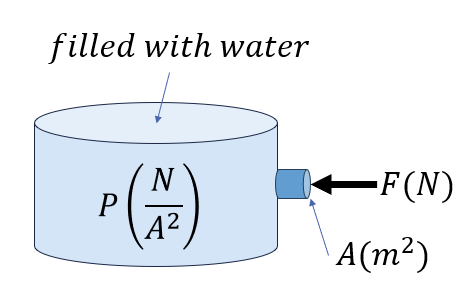
\includegraphics[width=3.85916in,height=1.66296in]{media/media/image27.png}

\textbf{איור 23 -- אטימת חור במיכל עם לחץ מים.} מקור: \emph{Flex Seal}.

{הלחץ הוא \textbf{מאפיין של הזרם עצמו}}, {ולא רק של נקודת המגע. במצב
מנוחה, המולקולות דוחפות אחת את השנייה כך שהלחץ בכל נקודה באותו עומק או
באותו מצב זרימה הוא זהה --- גם אם אין שם פתח או פקק ממשיים. לכן ניתן
לדבר על ``הלחץ במערכת'' או ``הלחץ בצינור'', כאילו היה זה גודל אחיד המתאר
את כל הזורם}.

יחידות הלחץ הן יחידות של כוח חלקי שטח. במערכת SI נהוג למדוד לחץ בפסקל
(Pa), כאשר

\[
1\,Pa = 1\,\frac{N}{m^{2}} = 1\,\frac{kg}{m\cdot s^{2}}
\]

יחידות נוספות נפוצות הן torr, atm ו־psi
\(\left(\frac{lb_{m}}{in^{2}}\right)\).

\subsubsection{\texorpdfstring{{לחץ
אטמוספירי}}{לחץ אטמוספירי}}\label{ux5dcux5d7ux5e5-ux5d0ux5d8ux5deux5d5ux5e1ux5e4ux5d9ux5e8ux5d9}

{באותו האופן האוויר שסביבנו מפעיל עלינו לחץ. האוויר הוא תערובת של גזים
שחלקיקיהם נעים ומתנגשים כל הזמן והתנגשויות אלה מפעילות כח עלינו ועל כל
מה שנמצא סביבנו.}

{הכוח הכולל שמפעילה האטמוספירה על כל יחידת שטח של פני הקרקע או של גוף
כלשהו נקרא \textbf{לחץ אטמוספירי}}.

{הלחץ האטמוספירי בגובה פני הים הוא בערך}:

\[P_{atm} = 1.013*10^{5}Pa = 1atm\]

{כלומר, האוויר שסביבנו מפעיל על כל מטר מרובע של הגוף שלנו כוח של
כקילוגרם אחד -- ואיננו מרגישים זאת רק משום שהלחץ בתוך גופנו שווה לזה
שבחוץ}. {אם נסתכל על פחית שתייה פתוחה "ריקה", אנו יודעים שהיא לא באמת
ריקה, אלא מכילה אוויר באותו הלחץ כמו האוויר שסביבנו. אם נחבר פחית זו
למשאבת ואקום כאשר נשאב את האויר מתוך הפחית, כבר לא תהיה התנגדות ללחץ
שהאויר שמחוץ לפחית מפעיל, והפחית תקרוס פנימה.}

\textbf{איור 24 -- פחית מחוברת למשאבת ואקום.} הוצאת האוויר גורמת ללחץ
האטמוספירי למעוך את הפחית פנימה.\\
נוצר בעזרת בינה מלאכותית (\emph{Nano Banana}, 2025).

{הלחץ האטמוספירי איננו קבוע בכל מקום}. {ככל שעולים לגובה רב יותר -- על
פני הר, במטוס או בבלון מזג אוויר -- יש \textbf{פחות שכבות אוויר
מעלינו}}, {ולכן גם \textbf{פחות משקל של אוויר הלוחץ כלפי מטה}}.\\
{התוצאה היא ירידה הדרגתית בלחץ האטמוספירי עם העלייה בגובה. לכן הלחץ
בגובה פני הים הוא כ-1 אטמוספירה, אך בגובה של כ־5 ק"מ (בערך מחצית גובה
האוורסט) הלחץ יורד כמעט למחצית מערכו}.{\hfill\break
כאשר אומרים לנו שאנו נמצאים בתנאים של לחץ אטמוספירי הכוונה היא} P=1atm

\textbf{איור 25 -- האטמוספירה בנויה משכבות של אוויר.} כל שכבה מפעילה
משקל על השכבות שמתחתיה, ולכן ככל שיורדים לגובה נמוך יותר - המולקולות
נדחסות והלחץ עולה בהתאם.\\
נוצר בעזרת בינה מלאכותית (\emph{Nano Banana}, 2025).

\subsection{\texorpdfstring{{לחץ
הידרוסטטי}}{לחץ הידרוסטטי}}\label{ux5dcux5d7ux5e5-ux5d4ux5d9ux5d3ux5e8ux5d5ux5e1ux5d8ux5d8ux5d9}

{בדומה לאטמוספירה, גם בתוך נוזל או גז הנמצא במנוחה הלחץ משתנה עם הגובה.
כל שכבה של זורם נושאת את משקל השכבות שמעליה, ולכן ככל שיורדים לעומק גדול
יותר -- כך גדל המשקל המצטבר מעל הנקודה, והלחץ עולה}. {}

Figure {26- לחץ הידרוסטטי של מים, ככל שהחריר בנקודה יותר נמוכה, הלחץ
גבוה יותר ולכן הזרימה החוצה מאותו החריר תהיה חזקה יותר.}

נניח עמוד זורם שגובהו \(h\), צפיפותו \(\rho\), והוא פתוח לאוויר.\\
הלחץ בראש העמוד יהיה הלחץ האטמוספירי (\(P_{0}\)), והלחץ בתחתית העמוד
יהיה:

\[
P = P_{0} + \frac{\rho g h}{g_{c}}
\]

זהו \textbf{הלחץ ההידרוסטטי} - הלחץ הנובע ממשקל הזורם עצמו.

{הנוסחה תקפה לכל זורם במנוחה, בין אם מדובר בשמן במיכל, במים בצינור או
באוויר בשכבות התחתונות של האטמוספירה}. {עיקרון זה מסביר תופעות רבות שאנו
פוגשים בחיי היומיום ובהנדסה}:\\
{מדוע צוללים חשים בלחץ גדל עם העומק, מדוע סכר נבנה עבה יותר בבסיסו,
ומדוע תחתית מיכל תעשייתי חייבת לעמוד בעומסים גדולים בהרבה מחלקו העליון}.

\subsubsection{\texorpdfstring{{ע֫ומד
(במלעיל)}}{ע֫ומד (במלעיל)}}\label{ux5e2ux5d5ux5deux5d3-ux5d1ux5deux5dcux5e2ux5d9ux5dc}

אחת הדרכים לביטוי לחץ היא לא ביחידות של כוח ליחידת שטח, אלא
כ\textbf{גובה שקול של זורם} שהיה מפעיל את אותו לחץ. נניח עמוד זורם בגובה
\(h\), בצפיפות \(\rho\). הלחץ בתחתיתו הוא \(P = \rho g h\). ניתן להביע
את הלחץ בתחתית העמוד באמצעות גובה נוזל מסוים (לרוב כספית או מים) שהיה
גורם לאותו הלחץ.

{{עומד לחץ} או {גובה שקול ללחץ (}}{head{),}}{והוא מבטא את הלחץ ביחידות
של אורך של נוזל.}

לחץ של ‎1‎ אטמוספירה ניתן לביטוי כעומד של ‎10.3‎ מטר מים או ‎760‎ מילימטר
כספית:

\[
1\,atm = 101325\,Pa = 760\,mmHg = 10.3\,mH_{2}O = 29.92\,inHg
\]

{אנו יכולים למצוא את העומד על ידי חלוקת הלחץ בצפיפות הנוזל הרצוי}

\[P_{head} = \frac{\rho_{fluid\ }\frac{g}{g_{c}}}{P\ \left( \frac{force}{area} \right)}\]

\begin{tcolorbox}[enhanced jigsaw, colback=white, arc=.35mm, coltitle=black, breakable, toptitle=1mm, leftrule=.75mm, colbacktitle=quarto-callout-note-color!10!white, opacitybacktitle=0.6, bottomtitle=1mm, titlerule=0mm, opacityback=0, colframe=quarto-callout-note-color-frame, title=\textcolor{quarto-callout-note-color}{\faInfo}\hspace{0.5em}{הערה}, rightrule=.15mm, bottomrule=.15mm, toprule=.15mm, left=2mm]

{יחידות העומד} (Head) {נראות במבט ראשון זהות ליחידות של \textbf{אורך -}
למשל מטרים או סנטימטרים - אך משמעותן הפיזיקלית שונה לחלוטין}. {כאשר אנו
אומרים ``גובה של 2 מטרים'', הכוונה היא למרחק פיזי במרחב}. {לעומת זאת,
כשאנחנו אומרים ``עומד לחץ של 2 מטר מים'', אין מדובר במרחק ממשי, אלא
ב\textbf{גובה שקול של עמוד מים שהיה יוצר את אותו לחץ}}.
\[P(mmHg) = P_{0}(mmHg) + h(mmHg)\] {כיצד נזהה שמדובר בעומד ולא באורך
אמיתי}?\\
{נבחן את \textbf{ההקשר הפיזיקלי} אם הגודל מופיע כחלק מביטוי של לחץ}
\((P = \rho gh)\) {ויחד עימו מוזכר נוזל מסויים (לרוב מים או כספית) --
מדובר בעומד}. {אם הוא מתאר מיקום במרחב (כמו גובה מיכל, אורך צינור או
מרחק בין נקודות) -- מדובר באורך}.

\end{tcolorbox}

\subsection{\texorpdfstring{{הבדלים בין גזים לנוזלים: צפיפויות והפרשי
גובה}}{הבדלים בין גזים לנוזלים: צפיפויות והפרשי גובה}}\label{ux5d4ux5d1ux5d3ux5dcux5d9ux5dd-ux5d1ux5d9ux5df-ux5d2ux5d6ux5d9ux5dd-ux5dcux5e0ux5d5ux5d6ux5dcux5d9ux5dd-ux5e6ux5e4ux5d9ux5e4ux5d5ux5d9ux5d5ux5ea-ux5d5ux5d4ux5e4ux5e8ux5e9ux5d9-ux5d2ux5d5ux5d1ux5d4}

ראינו כי בזורמים, הלחץ משתנה כתלות בעומק לפי המשוואה ההידרוסטטית:

\[P = P_0 + \rho g h\]

עם זאת, בהנדסת תהליכים נהוג לעיתים קרובות להניח כי הלחץ בתוך מכל המלא
בגז הוא אחיד בכולו, ללא תלות בגובה. מדוע אנו עושים זאת עבור גזים אך לא
עבור נוזלים?

ההבדל טמון ב\textbf{צפיפות (\(\rho\))}. צפיפותם של גזים נמוכה בדרך כלל
בסדרי גודל מצפיפותם של נוזלים (לרוב פי 1,000 בקירוב). כאשר אנו מציבים
ערך נמוך של צפיפות במשוואה ההידרוסטטית, התוספת ללחץ (\(\rho g h\)) הופכת
להיות קטנה מאוד, עד כדי כך שהיא זניחה עבור הפרשי גובה האופייניים לציוד
תעשייתי (מטרים בודדים עד עשרות מטרים).

\begin{tcolorbox}[enhanced jigsaw, colback=white, arc=.35mm, coltitle=black, breakable, toptitle=1mm, leftrule=.75mm, colbacktitle=quarto-callout-tip-color!10!white, opacitybacktitle=0.6, bottomtitle=1mm, titlerule=0mm, opacityback=0, colframe=quarto-callout-tip-color-frame, title=\textcolor{quarto-callout-tip-color}{\faLightbulb}\hspace{0.5em}{כלל אצבע הנדסי}, rightrule=.15mm, bottomrule=.15mm, toprule=.15mm, left=2mm]

\begin{itemize}
\tightlist
\item
  \textbf{בנוזלים:} השינוי בלחץ עם הגובה הוא משמעותי וחובה להתחשב בו.
\item
  \textbf{בגזים:} במערכות תעשייתיות סטנדרטיות, נזניח את השינוי בלחץ
  כתלות בגובה ונניח כי הלחץ אחיד בכל נפח הגז (אלא אם מדובר בהפרשי גובה
  אטמוספריים או במדידות מדויקות במיוחד).
\end{itemize}

\end{tcolorbox}

השוואה כמותית -- מיכל דו-פאזי כדי להבין את סדרי הגודל ולהצדיק את ההזנחה
של עמוד הגז, נבחן מיכל אחסון גבוה המכיל נוזל וגז.

\textbf{תיאור המערכת:} מיכל אחסון בגובה כולל של \(20\) מטרים מכיל מים
בחציו התחתון וחנקן (\(N_2\)) בחציו העליון.

\begin{itemize}
\tightlist
\item
  גובה עמוד המים: \(10\) מטרים.
\item
  גובה עמוד הגז (חנקן): \(10\) מטרים.
\item
  הלחץ הנמדד בראש המיכל (בנקודה הגבוהה ביותר) הוא
  \(P_{top} = 2 \text{ atm}\).
\end{itemize}

\textbf{נתונים:}

\begin{itemize}
\tightlist
\item
  צפיפות המים: \(\rho_{water} = 1000 \frac{kg}{m^3}\)
\item
  צפיפות החנקן (בתנאים אלו): \(\rho_{gas} \approx 1.2 \frac{kg}{m^3}\)
\end{itemize}

חשבו: א. מהו הלחץ במרכז המיכל (בממשק שבין הגז לנוזל)? ב. מהו הלחץ בתחתית
המיכל? ג. השוו את תוספת הלחץ שתרם עמוד הגז לעומת תוספת הלחץ שתרם עמוד
הנוזל.

\begin{tcolorbox}[enhanced jigsaw, colback=white, arc=.35mm, coltitle=black, breakable, toptitle=1mm, leftrule=.75mm, colbacktitle=quarto-callout-note-color!10!white, opacitybacktitle=0.6, bottomtitle=1mm, titlerule=0mm, opacityback=0, colframe=quarto-callout-note-color-frame, title=\textcolor{quarto-callout-note-color}{\faInfo}\hspace{0.5em}{פתרון}, rightrule=.15mm, bottomrule=.15mm, toprule=.15mm, left=2mm]

\textbf{א. חישוב הלחץ בממשק (תרומת עמוד הגז):}

נחשב את תוספת הלחץ ההידרוסטטי של הגז לאורך 10 מטרים:
\[\Delta P_{gas} = \rho_{gas} \cdot \frac{g}{g_c} \cdot h = 1.2 \frac{kg}{m^3} \cdot \frac{9.81 \frac{m}{s^2}}{1} \cdot 10 m = 117.7 \text{ Pa}\]

נמיר לאטמוספירות כדי להשוות ללחץ בראש המיכל:
\[\Delta P_{gas} = \frac{117.7}{101325} \approx 0.0011 \text{ atm}\]

הלחץ בממשק הוא הלחץ בראש המיכל ועוד התוספת:
\[P_{interface} = 2 + 0.0011 = 2.0011 \text{ atm}\]

\emph{אנו רואים שהשינוי בכלל לא נכנס בטווח הספרות המשמעותיות שאנו
מתייחסים אליהם.}

\textbf{ב. חישוב הלחץ בתחתית (תרומת עמוד הנוזל):}

כעת נחשב את תוספת הלחץ של עמוד המים (גם הוא בגובה 10 מטרים):
\[\Delta P_{liquid} = \rho_{water} \cdot \frac{g}{g_c} \cdot h = 1000 \frac{kg}{m^3} \cdot \frac{9.81 \frac{m}{s^2}}{1} \cdot 10 m = 98,100 \text{ Pa}\]

נמיר לאטמוספירות:
\[\Delta P_{liquid} = \frac{98100}{101325} \approx 0.968 \text{ atm}\]

הלחץ בתחתית הוא הלחץ בממשק ועוד תוספת הנוזל:
\[P_{bottom} = 2.0011 + 0.968 \approx 2.97 \text{ atm}\]

\textbf{ג. מסקנה:}

עבור אותו גובה בדיוק (\(10\) מטרים), עמוד הנוזל הוסיף כמעט \textbf{1
אטמוספירה} ללחץ, בעוד עמוד הגז הוסיף כ-\textbf{אלפית אטמוספירה} בלבד.

\end{tcolorbox}

\begin{tcolorbox}[enhanced jigsaw, colback=white, arc=.35mm, coltitle=black, breakable, toptitle=1mm, leftrule=.75mm, colbacktitle=quarto-callout-warning-color!10!white, opacitybacktitle=0.6, bottomtitle=1mm, titlerule=0mm, opacityback=0, colframe=quarto-callout-warning-color-frame, title=\textcolor{quarto-callout-warning-color}{\faExclamationTriangle}\hspace{0.5em}{ומה קורה כשהזורמים בתנועה?}, rightrule=.15mm, bottomrule=.15mm, toprule=.15mm, left=2mm]

חשוב להדגיש: ההזנחה שביצענו כעת מתייחסת לשינוי הלחץ הנובע מ\textbf{משקל
עמוד הגז בלבד} (הלחץ ההידרוסטטי, \(\rho g h\)). במערכות שבהן הגז
\textbf{זורם} בצינורות (במיוחד במהירויות גבוהות או למרחקים ארוכים), הלחץ
עשוי להשתנות באופן משמעותי בגלל \textbf{חיכוך} עם דפנות הצינור. בשלב זה
של הקורס אנו מתמקדים בלחצים סטטיים (מנוחה). כאשר נלמד על זרימה, נראה
כיצד לחשב גם את מפלי הלחץ הנובעים מזרימה של זורם. אולם הכלל נשאר תקף:
תרומת \textbf{הפרשי הגובה} ללחץ של גז היא כמעט תמיד זניחה, בין אם הוא
עומד ובין אם הוא זורם.

\end{tcolorbox}

\subsection{\texorpdfstring{{לחץ אטמוספירי, לחץ מוחלט ולחץ
יחסי}}{לחץ אטמוספירי, לחץ מוחלט ולחץ יחסי}}\label{ux5dcux5d7ux5e5-ux5d0ux5d8ux5deux5d5ux5e1ux5e4ux5d9ux5e8ux5d9-ux5dcux5d7ux5e5-ux5deux5d5ux5d7ux5dcux5d8-ux5d5ux5dcux5d7ux5e5-ux5d9ux5d7ux5e1ux5d9}

{עד עתה כשדיברנו על לחץ, התייחסנו ללחץ מוחלט - כלומר, לחץ שנמדד ביחס
לואקום - מצב בו אין צורונים כלל, ולכן אין התנגשויות ולא מופעל כח. אבל
למעט מקרים נדירים מופעל עלינו לחץ חיצוני קבוע - הלחץ האטמוספירי. במרבית
המדידות המכשירים יראו לנו את הלחץ היחסי} \emph{(Gauge Pressure)} {- הלחץ
הנמדד ביחס ללחץ האטמוספירי}\emph{.} {כאשר מד הלחץ מחובר לאוויר החופשי,
הוא מציג ערך אפס, מפני שהלחץ שבתוכו שווה בדיוק ללחץ האטמוספירה שמחוצה
לו}\emph{.} {רק כאשר הלחץ במערכת גדול או קטן מהלחץ החיצוני, המד מראה ערך
חיובי או שלילי בהתאמה}\emph{.}

{הקשר בין שני סוגי הלחץ הוא פשוט}\emph{:}

\[P_{abs} = P_{\text{gauge}} + P_{\text{atmospheric}}\] {כאשר}
\(P_{\text{gauge}} = 0\), {פירושו שהלחץ במערכת שווה ללחץ האטמוספירי}.

כאשר הערך שלילי, משמעות הדבר שהלחץ במערכת קטן מהלחץ האטמוספירי - מצב
הנקרא \textbf{ואקום חלקי}. במקרה זה מכשיר המדידה יראה ערך שלילי, והערך
הזה מייצג את ``עוצמת הואקום''. לדוגמה, אם המכשיר מראה ערך של
\(-100\,mmHg\), המשמעות היא שהלחץ האבסולוטי הוא \(660\,mmHg\), ויש לנו
ואקום של 10 ס''מ כספית.

\begin{tcolorbox}[enhanced jigsaw, colback=white, arc=.35mm, coltitle=black, breakable, toptitle=1mm, leftrule=.75mm, colbacktitle=quarto-callout-note-color!10!white, opacitybacktitle=0.6, bottomtitle=1mm, titlerule=0mm, opacityback=0, colframe=quarto-callout-note-color-frame, title=\textcolor{quarto-callout-note-color}{\faInfo}\hspace{0.5em}{הערה}, rightrule=.15mm, bottomrule=.15mm, toprule=.15mm, left=2mm]

\begin{itemize}
\tightlist
\item
  יחידות המיועדות רק ללחץ אבסולוטי: \textbf{atma}, \textbf{psia}\\
\item
  יחידות המיועדות רק ללחץ יחסי: \textbf{atmg}, \textbf{psig}\\
\item
  שאר היחידות (למשל \textbf{Pa} או \textbf{mmHg}) דורשות ציון מפורש\\
\item
  אם אין ציון מפורש, ניתן להניח שמדובר בלחץ אבסולוטי
\end{itemize}

\end{tcolorbox}

\subsubsection{\texorpdfstring{{ברומטר ולחץ
ברומטרי}}{ברומטר ולחץ ברומטרי}}\label{ux5d1ux5e8ux5d5ux5deux5d8ux5e8-ux5d5ux5dcux5d7ux5e5-ux5d1ux5e8ux5d5ux5deux5d8ux5e8ux5d9}

{כשאין מידע נוסף אנו מעריכים את הלחץ החיצוני המופעל עלינו כלחץ של}
1atm{. אך הלחץ המדוייק תלוי בתנאים שבהם אנו נמצאים כמו הגובה מעל (או
מתחת) פני הים והטמפ\textquotesingle{} שאנו נמצאים בה. על מנת למדוד את
הלחץ המופעל עלינו על ידי האטמוספירה בפועל בנקודה מסויימת בזמן מסויים,}
{נשתמש במכשיר שנקרא {ברומטר}}{(Barometer){.}} {}

{ברומטר כספית הוא מכשיר פשוט אך מדויק למדידת הלחץ על פני השטח. הוא מורכב
מצינור זכוכית ארוך (בדרך כלל באורך של כ־90 ס״מ), שצידו האחד אטום וסגור},
{והצד השני פתוח ומוטבל בתוך כלי המכיל כספית נוזלית}. {את הצינור ממלאים
לחלוטין בכספית, סוגרים את קצהו העליון, והופכים אותו כך שקצהו הפתוח ייטבל
במיכל}. {כאשר הצינור מונח כך, חלק מהכספית מחליקה החוצה אל המיכל, אך רובה
נותרת בצינור}. {בחלק העליון של הצינור נוצר חלל כמעט ריק} -- {ואקום כמעט
מושלם} -- {משום שאין בו אוויר כלל}. {במצב זה נוצר שיווי משקל בין שני
כוחות}: {הלחץ שמפעיל האוויר האטמוספירי על פני הכספית שבמיכל} ,{ומשקל
עמוד הכספית שבתוך הצינור}. {שיווי המשקל מתואר על ידי}:

\[P_{\text{barometer}} = \frac{\rho_{\text{Hg}}gh}{g_{c}}\]

כאשר h הוא גובה עמוד הכספית הנותר בצינור.

{מאחר והחלל שבחלק העליון של הצינור הוא למעשה וואקום, הלחץ בראש עמוד
הכספית כמעט אפסי}.\\
{מכאן שהלחץ הנמדד בברומטר הוא לחץ מוחלט ביחס לוואקום זה, וניתן להשתמש בו
כערך הייחוס (לחץ ברומטרי) לכל חישוב של לחצים יחסיים במכשירים אחרים}.

\[P_{abs} = P_{\text{gauge}} + P_{\text{barometer}}\]

הסטודנטית החרוצה סתוונית אחראית על בדיקת תקינות מיכל גז במפעל בו היא
עובדת.\\
מד הלחץ (\emph{Gauge}) המותקן על המכל מראה \(200\,kPa\).\\
הלחץ האטמוספירי באותו היום נמדד בברומטר כספית ועמד על \(720\,mmHg\).\\
ידוע כי המכל מתוכנן לעמוד בלחץ אבסולוטי מרבי של \(310\,kPa\).

האם המכל נמצא בתחום התקין או שקיים חשש לחריגה מהלחץ המותר?

\subsection{\texorpdfstring{. {מכשירים למדידת
לחץ}}{. מכשירים למדידת לחץ}}\label{ux5deux5dbux5e9ux5d9ux5e8ux5d9ux5dd-ux5dcux5deux5d3ux5d9ux5d3ux5ea-ux5dcux5d7ux5e5}

{קיימות שיטות רבות למדידת לחץ, השונות זו מזו בעקרון הפעולה, בטווחי
הלחצים המתאימים ובדיוק הנדרש}. {לפי} \emph{Perry's Chemical Engineers'
Handbook{,}} {ניתן לחלק את מכשירי המדידה לשלוש קבוצות עיקריות}:

\begin{enumerate}
\def\labelenumi{\arabic{enumi}.}
\item
  \textbf{{שיטות מבוססות עמוד נוזל} (liquid-column methods)} -- {כמו
  המנומטר, שבהן הלחץ נמדד באמצעות גובה נוזל המאזן את הלחץ הפועל עליו.
  שיטות אלו פשוטות, מדויקות יחסית ומתאימות במיוחד למדידות לחץ נמוך}.
\item
  \textbf{{שיטות אלסטיות} (elastic-element methods)} -- {מבוססות על
  עיוות מכני של רכיב מתכתי אלסטי, כמו בצינור בורדון, בדיאפרגמה או במפוח.
  הלחץ גורם לעיוות מבוקר שמומר לתנועה מכנית הניתנת לקריאה על גבי סקלת
  מד. שיטות אלו נפוצות בתעשייה למדידת לחצים בינוניים וגבוהים}.
\item
  \textbf{{שיטות חשמליות} (electrical methods)} -- {משתמשות בחיישנים
  אלקטרוניים} ({כגון} strain gauges {או חיישנים פייזו־אלקטריים}),
  {הממירים את העיוות המכני לאות חשמלי. שיטות אלו מאפשרות מדידה מדויקת
  ורציפה, ומתאימות במיוחד למערכות בקרה אוטומטיות}.
\end{enumerate}

{שלוש הקטגוריות הללו מתבססות על עקרון משותף: הפיכת הלחץ הפועל לגודל מדיד
-- גובה נוזל, תזוזה מכנית, או אות חשמלי -- הניתן לכיול ביחידות של פסקל,
בר או אטמוספירה}.

\subsubsection{\texorpdfstring{{שיטות אלסטיות למדידת
לחץ}}{שיטות אלסטיות למדידת לחץ}}\label{ux5e9ux5d9ux5d8ux5d5ux5ea-ux5d0ux5dcux5e1ux5d8ux5d9ux5d5ux5ea-ux5dcux5deux5d3ux5d9ux5d3ux5ea-ux5dcux5d7ux5e5}

{בשיטות אלסטיות נמדד הלחץ באמצעות {עיוות מכני של רכיב מתכתי
אלסטי}}\textbf{.} {כאשר נוזל או גז מפעילים לחץ על רכיב גמיש --- כמו
צינור דק, קרום מתכת או מפוח --- הלחץ גורם לשינוי בצורתו. שינוי זה מומר
לתנועה מדידה, לרוב באמצעות מנגנון מכני פשוט המחובר למחוג או חיישן}.
{השיטה הנפוצה ביותר היא {צינור בורדון}}{(Bourdon tube)}{\textbf{.} צינור
זה בנוי מצינור מתכתי קעור בעל חתך אליפטי, המעוקל בצורת חצי עיגול או
סליל. הקצה הפתוח של הצינור מחובר אל מקור הלחץ, בעוד שהקצה השני סגור
ויכול לנוע בחופשיות}. {כאשר הלחץ הפנימי בצינור עולה, דפנות הצינור נמתחות
והצורה הקמורה נוטה להתיישר. תנועה קטנה זו מועברת באמצעות מנגנון של מנוף
וגלגל שיניים אל מחוג המורה את הלחץ על גבי סקלת המד}.

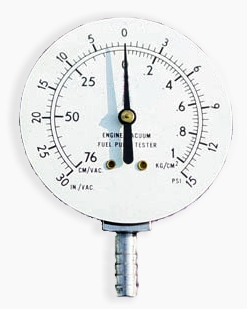
\includegraphics[width=2.05088in,height=2.56567in]{media/media/image31.jpg}
{}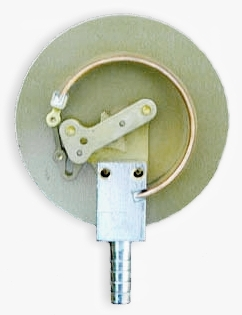
\includegraphics[width=1.98575in,height=2.58476in]{media/media/image32.jpg}

\textbf{איור 27 -- מד לחץ מסוג בורדון (Bourdon Gauge).} מימין: מראה
חיצוני של מד הלחץ, שבו תנועת המחוג מציגה את ערך הלחץ על גבי סולם
מכויל.\\
משמאל: מבט פנימי של מנגנון המדידה -- צינור מתכתי קמור בצורת C (צינור
בורדון) המחובר לקו הלחץ. מקור: ויקיפדיה

{מדי לחץ מסוג בורדון פשוטים, אמינים, ואינם דורשים מקור אנרגיה חיצוני. הם
מתאימים למדידה של {לחץ מדומה}} {(Gauge Pressure)} {ומספקים תוצאות
מדויקות בטווח רחב מאוד של לחצים, החל ממאות קילו־פסקל ועד מאות מגה־פסקל}.
{חסרונם העיקרי הוא רגישות לשינויים מהירים בלחץ ולבלאי מכני לאורך זמן}.
{בזכות פשטותם ואמינותם, מדי בורדון נחשבים עד היום לאחד המכשירים הנפוצים
ביותר למדידת לחץ במערכות תעשייתיות, במעבדות ובמתקני בקרה}.

{מלבד צינור בורדון, קיימות שיטות נוספות למדידת לחץ המבוססות על אותו
עיקרון של עיוות אלסטי של רכיב מתכתי}. {במכשירי דיאפרגמה הלחץ מפעיל כוח
על קרום מתכתי דק המתעוות בהתאם לעוצמת הלחץ, ובמכשירי מפוח} (bellows)
{הלחץ גורם להתפשטות או כיווץ של גליל מתקפל דק}. {בכל המקרים מדובר בהמרה
של שינוי מכני קטן --- כיפוף, מתיחה או התרחבות --- לתנועה מדידה, אשר
מתורגמת להצגה אנלוגית או לאות חשמלי}. {מכשירים אלה מאפשרים מדידה מדויקת
גם בטווחי לחץ שונים מאוד, החל מהפרשי לחץ זעירים ועד ללחצים גבוהים
בתעשייה, והם מהווים את הבסיס למרבית מדי הלחץ המכניים המודרניים}.

\subsubsection{\texorpdfstring{{שיטות חשמליות למדידת
לחץ}}{שיטות חשמליות למדידת לחץ}}\label{ux5e9ux5d9ux5d8ux5d5ux5ea-ux5d7ux5e9ux5deux5dcux5d9ux5d5ux5ea-ux5dcux5deux5d3ux5d9ux5d3ux5ea-ux5dcux5d7ux5e5}

{בשיטות חשמליות נמדד הלחץ בעזרת חיישנים ההופכים עיוות מכני לאות חשמלי
מדיד}. {בכל השיטות העיקרון זהה: לחץ הפועל על רכיב גמיש גורם לשינוי פיזי
(כיפוף, מתיחה או דחיסה), והמערכת האלקטרונית מתרגמת שינוי זה לשינוי במתח,
בזרם או במטען}. {היתרון המרכזי של שיטות אלו הוא האפשרות לשלב אותן
במערכות בקרה ממוחשבות, ולקבל מדידה רציפה, מדויקת ומהירה של לחצים גם
בתנאים משתנים}. {קיימים שלושה סוגים עיקריים של חיישנים חשמליים}:

\begin{itemize}
\item
  {}Strain Gauge {- חוט מתכתי דק או סרט מוליך שההתנגדות החשמלית שלו
  משתנה בהתאם למידת המתיחה או הדחיסה. שינוי ההתנגדות מומר ישירות לשינוי
  במתח החשמלי ומאפשר מדידת לחצים סטטיים לאורך זמן}.
\item
  Piezo-resistive Sensor {- מבוסס על שינוי בהתנגדות החשמלית של חומרים
  מוליכים למחצה (כמו סיליקון) כתוצאה מלחץ מכני. חיישנים אלה רגישים
  במיוחד ומתאימים למערכות מדידה מדויקות, כולל יישומים רפואיים
  ותעשייתיים}.
\item
  Piezo-electric Sensor {-} {מבוסס על תופעת הפייזואלקטריות, שבה גבישים
  מסוימים (כמו קוורץ או חומרים קרמיים) מייצרים מטען חשמלי חדש כשהם
  נתונים ללחץ. המטען מומר לאות חשמלי באמצעות מעגל הגברה, ומאפשר מדידה של
  לחצים דינמיים מאוד -- כמו פיצוצים, רטט או פעימות מהירות במנועים}.
  {}~{יש לציין כי חיישנים אלו אינם מתאימים למדידת לחץ סטטי (קבוע) לאורך
  זמן, כיוון שהמטען החשמלי נוטה להתפוגג.}
\end{itemize}

{החיישנים החשמליים משלבים בין רגישות גבוהה}, {מהירות תגובה ויכולת
אינטגרציה במערכות בקרה מתקדמות}. {עם זאת, יש להבחין בין חיישנים המתאימים
ללחצים קבועים לבין כאלה המשמשים למדידות רגעיות בלבד -- בהתאם לעקרון
הפעולה של כל טכנולוגיה}.

\subsection{\texorpdfstring{{מנומטרים}}{מנומטרים}}\label{ux5deux5e0ux5d5ux5deux5d8ux5e8ux5d9ux5dd}

\textbf{{מנומטרים} (Manometers)} {הם מהמכשירים הפשוטים והמדויקים ביותר
למדידת לחץ}. {הם פועלים על עקרון בסיסי של שיווי משקל הידרוסטטי: כאשר
עמודת נוזל נמצאת במנוחה, הפרש הגבהים בין שני צדדים של הצינור משקף את
הפרש הלחצים ביניהם}. {מנומטר טיפוסי הוא צינור בצורת} U {המכיל נוזל מדידה
(כמו כספית או מים). כאשר שני צדדיו חשופים ללחצים שונים, הנוזל נע עד
שהפרשי הלחצים משתווים להפרש המשקלים של עמודות הנוזל בשני הצדדים. גובה
עמודת הנוזל מהווה מדד ישיר להפרש הלחצים בין הנקודות}.

\subsubsection{\texorpdfstring{{משוואת המנומטר
הכללית}}{משוואת המנומטר הכללית}}\label{ux5deux5e9ux5d5ux5d5ux5d0ux5ea-ux5d4ux5deux5e0ux5d5ux5deux5d8ux5e8-ux5d4ux5dbux5dcux5dcux5d9ux5ea}

העיקרון הפיזיקלי הבסיסי הוא שהלחץ זהה בכל שתי נקודות הנמצאות באותו גובה
באותו נוזל רציף.\\
נניח שני לחצים בשני הקצוות, \(P_{1}\) ו־\(P_{2}\), ושני זורמים בצינור --
נוזל מדידה בצפיפות \(\rho_{1}\) וזורם (לרוב אוויר) בצפיפות \(\rho_{2}\).

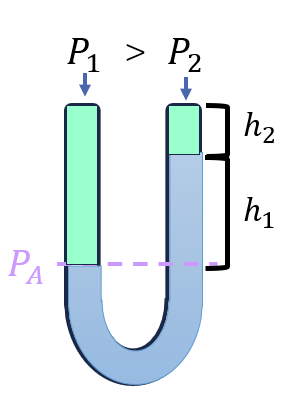
\includegraphics[width=1.41in,height=2.02in]{media/media/image33.png}

\textbf{איור 28 -- משוואת המנומטר הכללית.} נוזל המדידה מסומן בכחול (לרוב
מים או כספית), הזורם העליון בירוק (לרוב אוויר, זניח), והלחצים החיצוניים
הם \(P_{1}\) ו־\(P_{2}\).

{אם נעקוב לאורך הצינור מצד 1, דרך נוזל המדידה, ועד לצד 2 -- נוכל להשוות
את הלחצים בנקודות שבאותו גובה}.\\
{נכתוב את הלחץ בכל זרוע ונשווה ביניהם} {וקיבלנו את}

{משוואת המנומטר הכללית}
\[P_{1} + \rho_{2}\frac{g}{g_{c}}(h_{1} + h_{2}) = P_{2} + \rho_{1}\frac{g}{g_{c}}h_{1} + \rho_{2}\frac{g}{g_{c}}h_{2}\]
{המתארת את הקשר בין הלחצים, צפיפויות הנוזלים והפרשי הגבהים בצינור}.

{במרבית היישומים הזורם העליון הוא גז (לרוב אוויר), שצפיפותו קטנה בהרבה
מצפיפות נוזל המדידה}.\\
{במקרה זה ניתן להזניח את תרומתו, ואז נקבל את}

{משוואת המנומטר כאשר הצפיפות של הזורם העליון זניחה:}
\[P_{1} - P_{2} = \rho\frac{g}{g_{c}}h\] כאשר \(\rho\) היא צפיפות נוזל
המדידה בלבד.

אם \(h > 0\) - הלחץ בצד 1 גבוה יותר; אם \(h < 0\) - הלחץ בצד 2 גבוה
יותר.

נוסחה זו היא הצורה הפשוטה והנפוצה של \textbf{משוואת המנומטר}. אם אחד
הצדדים של המנומטר פתוח לאטמוספירה, ניתן להשתמש בו למדידת לחץ יחסי
(\emph{Gauge Pressure}), ואם שני הצדדים מחוברים לנקודות שונות במערכת -
הוא מודד \textbf{הפרש לחצים} (\emph{Differential Pressure}). מנומטרים
משמשים בעיקר ביישומים שבהם נדרש דיוק גבוה בטווחי לחץ נמוכים, כמו כיול
חיישנים, ניסויי זרימה במעבדה או מדידות בפרויקטים חינוכיים. לעומת זאת,
במערכות תעשייתיות בלחצים גבוהים משתמשים לרוב במדי לחץ אלסטיים או
אלקטרוניים, שהם קומפקטיים ועמידים יותר.

{נתונה המערכת הבאה:\\
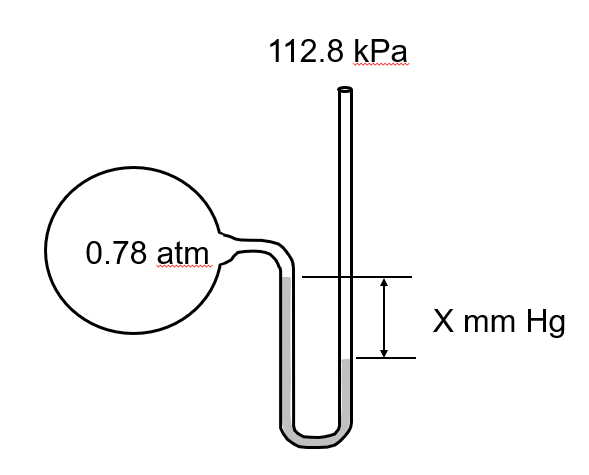
\includegraphics[width=2.01046in,height=1.62134in]{media/media/image34.png}
1. באיזה צד הלחץ יותר גבוה?\\
2. מהו} h{?}

\subsubsection{\texorpdfstring{{סוגי
מנומטרים}}{סוגי מנומטרים}}\label{ux5e1ux5d5ux5d2ux5d9-ux5deux5e0ux5d5ux5deux5d8ux5e8ux5d9ux5dd}

Figure {29}- {סוגי מנומטרים}

\textbf{{מנומטר פתוח} \emph{(Open-End Manometer)}}

במנומטר פתוח צד אחד של הצינור חשוף לאטמוספירה, והצד השני מחובר לנקודה
במערכת שבה נרצה למדוד את הלחץ. אם הלחץ במערכת גדול מהלחץ האטמוספירי -
מפלס הנוזל בצד הפתוח יעלה; ואם הוא קטן - יירד.

\begin{itemize}
\item
  מאחר והמנומטר פתוח לאטמוספירה, הוא מראה את הלחץ היחסי
  (\emph{gauge}):\\
  \(P_{1g} = \rho \frac{g}{g_{c}} h\)
\item
  אם נרצה לדעת את הלחץ האבסולוטי בצינור, נצטרך להוסיף את הלחץ
  האטמוספירי:\\
  \[P_{1a} = P_{atm} + P_{1g} = P_{atm} + \rho\frac{g}{g_{c}}h\]
\end{itemize}

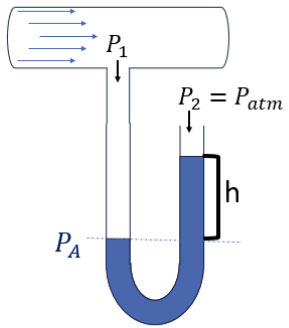
\includegraphics[width=1.50808in,height=1.7116in]{media/media/image36.png}

\textbf{{מנומטר סגור} \emph{(Sealed-End Manometer)}}

{במנומטר סגור צד אחד של הצינור אטום ומכיל ריק כמעט מוחלט}
\emph{(Vacuum)}{,} {והצד השני מחובר למערכת. מכיוון שבצד האטום הלחץ אפסי
בקירוב, הלחץ הנמדד הוא לחץ מוחלט}

\[P_{1a} = 0 + \rho\frac{g}{g_{c}}h\]
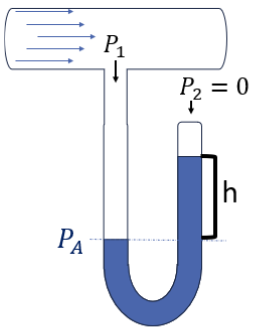
\includegraphics[width=1.34823in,height=1.69815in]{media/media/image37.png}

\textbf{{מנומטר דיפרנציאלי} \emph{(Differential Manometer)}}

{במנומטר דיפרנציאלי שני הצדדים מחוברים לשתי נקודות שונות במערכת}\emph{.*
{המכשיר מודד ישירות את \textbf{הפרש הלחצים} בין שתי הנקודות, ללא קשר
ללחץ האטמוספרי}}.*

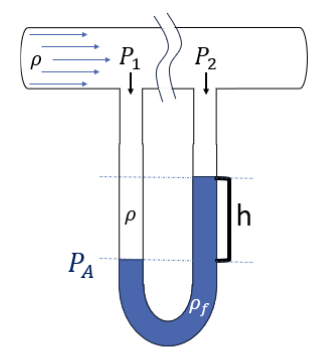
\includegraphics[width=1.55713in,height=1.73623in]{media/media/image38.png}

\[P_{1} + \rho\frac{g}{g_{c}}h = P_{2} + \rho_{f}\frac{g}{g_{c}}h\ \ \ \  \Longrightarrow \ \ \ \ \ \ \boxed{\mathrm{\Delta}P = P_{1} - P_{2} = \left( \rho_{f} - \rho \right)\frac{g}{g_{c}}h\text{~}}\]
כאשר \(\rho_{f}\) היא צפיפות נוזל המדידה ו־\(\rho\) היא צפיפות הזורם
במערכת.\\
אם צפיפות הזורם נמוכה משמעותית מצפיפות נוזל המנומטר (למשל אם מדובר
באוויר), נקבל:

\[
P_{1} - P_{2} = \rho \frac{g}{g_{c}} h
\]

\textbf{{מנומטר משופע} \emph{(Inclined Manometer)}}

במנומטר משופע אחת הזרועות של הצינור איננה אנכית אלא מונחת בזווית קטנה
ביחס לאופק. העיקרון הפיזיקלי זהה לזה של מנומטר רגיל, אך השיפוע מאפשר
למדוד שינויים קטנים מאוד בלחץ בדיוק גבוה יותר.

על כן, בהנחה שצפיפות הזורם במערכת זניחה:

\[
\Delta P = \rho \frac{g}{g_{c}} h = \rho \frac{g}{g_{c}} L \sin(\theta)
\]

כאשר \(L\) הוא המרחק הנמדד לאורך הצינור ו־\(\theta\) היא זווית ההטיה.
ככל ש־\(\theta\) קטנה יותר, נוכל להבחין בשינויים קטנים יותר בלחץ.

{}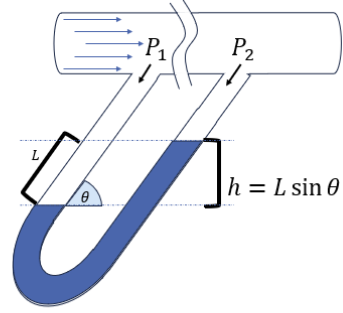
\includegraphics[width=2.14656in,height=1.95881in]{media/media/image39.png}

\textbf{{מנומטר עם צד רחב} \emph{(Large-Reservoir Manometer)}}

{במנומטר זה אחת הזרועות רחבה בהרבה מהשנייה}\emph{.* {כאשר הלחץ משתנה,
מפלס הנוזל בצד הצר נע מעלה או מטה באופן מורגש, בעוד שהשינוי במאגר הרחב
קטן משמעותית. לכן, יש להתחשב ביחס בין שטחי החתך של שני הצדדים}},*
\(A_{1}\){ו־}\(A_{2}\) {כדי לתקן את החישוב}\emph{.}

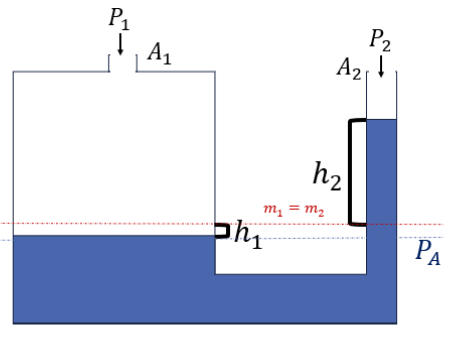
\includegraphics[width=3.13211in,height=2.4029in]{media/media/image40.png}

{אנו יודעים כי המסה שירדה בצד אחד חייבת להיות שווה למסה שעלתה בצד השני.
לכן, אם נסתכל על הנפח שעלה וירד ביחס לקו האדום -}

\[m_{1} = m_{2}\ \ ;\ \ \ m = \rho V\]

\[V_{1} = A_{1}h_{1}\ \ \ \ \ \ V_{2} = A_{2}h_{2}\]

\[m_{1} = \rho A_{1}h_{1}\ \ \ \ ;\ \ \ m_{2} = \rho A_{2}h_{2}\  \Rightarrow \ \rho A_{1}h_{1} = \rho A_{2}h_{2}\  \Rightarrow h_{1} = h_{2}\frac{A_{2}}{A_{1}}\]

** {כדי לחשב את הלחץ} \(P_{1}\) {נניח כי צפיפות האויר זניחה, וכי הצד
השני של המנומטר פתוח לאטמוספירה}

\[P_{1} = P_{2} + \rho\frac{g}{g_{c}}\left( h_{1} + h_{2} \right)\]

\[\boxed{P_{1} = P_{atm} + \rho\frac{g}{g_{c}}h_{2}\left( 1 + \frac{A_{2}}{A_{1}} \right)}\]

{אם המאגר רחב מאוד יחסית לצינור הצר, ניתן להגיד ש}
\(A_{1} \gg A_{2},\ h_{1} \ll h_{2}\) {והמשוואה מתלכדת עם המשוואה של
מנומטר רגיל.}

\[P_{1} = P_{atm} + \rho\frac{g}{g_{c}}h_{2}\left( 1 + \frac{A_{2}}{A_{1}} \right) = P_{atm} + \rho\frac{g}{g_{c}}h_{2}\]

{מבנה זה מאפשר \textbf{מדידה נוחה וקריאה מדויקת של הפרש גבהים}}\emph{,}
{כיוון שהשינוי מתרכז כולו בצינור הצר}\emph{.} {מנומטרים כאלה נפוצים
במעבדות ובמדידות כיול, שבהן נדרשת רגישות גבוהה אך שינוי לחץ
מוגבל}\emph{.}

\subsubsection{\texorpdfstring{{סיכום
מנומטרים}}{סיכום מנומטרים}}\label{ux5e1ux5d9ux5dbux5d5ux5dd-ux5deux5e0ux5d5ux5deux5d8ux5e8ux5d9ux5dd}

{מנומטרים הם מהמכשירים הפשוטים, המדויקים והמהימנים ביותר למדידת לחצים
והפרשי לחצים}.\\
{הם מבוססים על עקרון \textbf{שיווי המשקל ההידרוסטטי}}, {שלפיו הלחץ בנוזל
במנוחה תלוי רק בצפיפותו, בתאוצת הכובד ובגובה עמודת הנוזל}.\\
{הפרש הגבהים בין פני הנוזל בשתי זרועות הצינור מתורגם ישירות להפרש לחצים
על־פי המשוואה}: \[\Delta P = \rho gh\] {צורתו של המנומטר -- פתוח, סגור,
דיפרנציאלי, משופע או עם צד רחב -- נקבעת לפי סוג המדידה הרצויה: לחץ
מוחלט, לחץ יחסי או הפרש לחצים בין שני מקומות במערכת}. {למרות פשטותם,
מנומטרים משמשים עד היום במעבדות, בבדיקות כיול ובמערכות בקרה, בזכות רמת
הדיוק הגבוהה והיכולת לספק מדידה ישירה וברורה של לחץ באמצעות גובה עמודת
נוזל}.

{במכון הנדסי נתון מיכל מלבני ברוחב} \(1.0\text{~}m\) {ואורך}
\(3.0\text{~}m\){.}\\
{המיכל מלא עד לגובה} \(5.0\text{~}m\) {בחומר} Methyl Ethyl Ketone
(MEK){.}\\
{נתון:} \(S.G = 0.805\){.\\
הלחץ האטמוספירי באותו יום הוא} \(772\text{~}mmHg\){.}

\begin{enumerate}
\def\labelenumi{\arabic{enumi}.}
\tightlist
\item
  חשבו את הכח הפועל על תחתית המיכל\\
\item
  מהו העומד ביחידות של mMEK?\\
\item
  באחד הימים ירד גשם ונכנסו מים למיכל. יש לנו מד לחץ בתחתית הכלי, כיצד
  ניתן לחשב כמה מים נכנסו למיכל?\\
\item
  כיצד ניתן להחזיר את המיכל למצבו המקורי (ללא המים)?
\end{enumerate}

\begin{tcolorbox}[enhanced jigsaw, colback=white, arc=.35mm, coltitle=black, breakable, toptitle=1mm, leftrule=.75mm, colbacktitle=quarto-callout-note-color!10!white, opacitybacktitle=0.6, bottomtitle=1mm, titlerule=0mm, opacityback=0, colframe=quarto-callout-note-color-frame, title=\textcolor{quarto-callout-note-color}{\faInfo}\hspace{0.5em}{פתרון סעיף א}, rightrule=.15mm, bottomrule=.15mm, toprule=.15mm, left=2mm]

נתונים: מיכל מלבני: רוחב \(W = 1.0 \text{ m}\), אורך
\(L = 3.0 \text{ m}\) ולכן שטח תחתית \(A = WL = 3.0 \text{ m}^2\)

גובה נוזל: \(H = 5.0 \text{ m}\)

נוזל (MEK):
\[SG = 0.805 \Rightarrow \rho_{MEK} = 0.805 \cdot 1000 \text{ kg/m}^3 = 805 \text{ kg/m}^3\]

תאוצת הכובד: \(g = 9.8 \text{ m/s}^2\)

לחץ אטמוספרי: \[
P_{atm} = 772 \text{ mmHg} \times \frac{101325 \text{ Pa}}{760 \text{ mmHg}} = 1.029 \times 10^5 \text{ Pa}
\] א. הכוח על תחתית המיכל

הלחץ בתחתית (מוחלט): \(P_b = P_{atm} + \rho_{MEK} g H\)

הכוח על התחתית: \(F = P_b \cdot A\)

חישוב הלחץ ההידרוסטטי: \[
\Delta P = \rho_{MEK} g H = \frac{805 \text{ kg}}{\text{m}^3} \cdot 9.8 \frac{\text{m}}{\text{s}^2} \cdot 5.0 \text{ m} = 3.9485 \times 10^4 \frac{\text{kg}}{\text{m s}^2} = 3.9485 \times 10^4 \frac{\text{N}}{\text{m}^2}
\]

חישוב הלחץ בתחתית: \[
P_b = 1.029 \times 10^5 + 3.9485 \times 10^4 = 1.424 \times 10^5 \text{ Pa}
\]

חישוב הכוח הסופי: \[
\boxed{F = P_b A = 1.424 \times 10^5 \frac{\text{N}}{\text{m}^2} \cdot 3.0 \text{ m}^2 = 4.3 \times 10^5 \text{ N}}
\]

\end{tcolorbox}

\begin{tcolorbox}[enhanced jigsaw, colback=white, arc=.35mm, coltitle=black, breakable, toptitle=1mm, leftrule=.75mm, colbacktitle=quarto-callout-note-color!10!white, opacitybacktitle=0.6, bottomtitle=1mm, titlerule=0mm, opacityback=0, colframe=quarto-callout-note-color-frame, title=\textcolor{quarto-callout-note-color}{\faInfo}\hspace{0.5em}{פתרון סעיף ב}, rightrule=.15mm, bottomrule=.15mm, toprule=.15mm, left=2mm]

לחץ gauge בתחתית ביחידות של \(m\text{MEK}\)

לחץ \(gauge\) בתחתית ביחידות של \(m\text{MEK}\). לחץ \(gauge\) הוא למעשה
תרומת עמודת הנוזל בלבד. אנחנו רוצים להביע את העומד באמצעות יחידות של
\(m\text{MEK}\). במילים אחרות אנו עונים על השאלה מהו הגובה של
\(\text{MEK}\) שמפעיל לחץ כזה? הגובה הוא \(5.0\text{m}\) ולכן עומד הלחץ
הוא \(5.0\text{mMEK}\) (שווה ערך ל-\(3.95 \times 10^4 \text{ Pa}\)).

\end{tcolorbox}

\begin{tcolorbox}[enhanced jigsaw, colback=white, arc=.35mm, coltitle=black, breakable, toptitle=1mm, leftrule=.75mm, colbacktitle=quarto-callout-note-color!10!white, opacitybacktitle=0.6, bottomtitle=1mm, titlerule=0mm, opacityback=0, colframe=quarto-callout-note-color-frame, title=\textcolor{quarto-callout-note-color}{\faInfo}\hspace{0.5em}{פתרון סעיף ג}, rightrule=.15mm, bottomrule=.15mm, toprule=.15mm, left=2mm]

מה \(SG\) אנו יודעים שמים צפופים יותר מה-\(\text{MEK}\) ו לכן ייווצרו
שתי שכבות: מים בתחתית, \(\text{MEK}\) למעלה. מד הלחץ בתחתית מודד את ה
\(gauge\) הנוצר מסך הנוזל שמעליו. אנו יודעים מהו הלחץ שה \(\text{MEK}\)
יוצר, ולכן ההפרש בין ה \(gauge\) ללחץ של ה\(\text{MEK}\) יתן לנו בדיוק
את הלחץ של עמודת המים. מאחר ואנו יודעים את צפיפות המים ואת השטח של המיכל
נוכל לחשב את גובה המים היוצר את הלחץ הזה. או לחילופין, לחשב את עומד המים
הנובע מהפרש זה.

\end{tcolorbox}

\begin{tcolorbox}[enhanced jigsaw, colback=white, arc=.35mm, coltitle=black, breakable, toptitle=1mm, leftrule=.75mm, colbacktitle=quarto-callout-note-color!10!white, opacitybacktitle=0.6, bottomtitle=1mm, titlerule=0mm, opacityback=0, colframe=quarto-callout-note-color-frame, title=\textcolor{quarto-callout-note-color}{\faInfo}\hspace{0.5em}{פתרון סעיף ד}, rightrule=.15mm, bottomrule=.15mm, toprule=.15mm, left=2mm]

לצורך הוצאת המים מהמיכל, אנו יודעים מהפרש הצפיפויות שהמים הם השכבה
התחתונה, ולכן ניתן לרוקן בעדינות דרך פתח ניקוז תחתון את כל המים עד
שמגיעים לתחילת שכבת ה\(\text{MEK}\).

\end{tcolorbox}

\subsection{\texorpdfstring{{סיכום}}{סיכום}}\label{ux5e1ux5d9ux5dbux5d5ux5dd-5}

\begin{itemize}
\tightlist
\item
  לחץ הוא הכוח הפועל בניצב ליחידת שטח: \(P = \frac{F}{A}\)
\item
  לחץ בזורם הוא הכוח שהנוזל או הגז מפעיל בניצב על כל יחידת שטח שבתוכו או
  על גבולות הכלי המכיל אותו.
\item
  לחץ נוזל במנוחה עולה עם העומק בהתאם לצפיפות הנוזל ולכוח הכובד:
  \(\Delta P = \rho \frac{g}{g_{c}} h\)
\item
  \textbf{עומד (Head)} הוא הגובה השקול של עמודת נוזל שמייצרת לחץ נתון --
  כלומר, גובה עמוד הנוזל שהיה יוצר את אותו לחץ במנוחה.
\item
  \textbf{סוגי לחצים:}

  \begin{itemize}
  \tightlist
  \item
    \textbf{לחץ מוחלט (Absolute Pressure):} נמדד מה־\emph{Vacuum}.
  \item
    \textbf{לחץ אטמוספירי (Atmospheric Pressure):} לחץ האוויר שמסביבנו.
  \item
    \textbf{לחץ יחסי (Gauge Pressure):} ההפרש בין הלחץ המוחלט ללחץ
    האטמוספירי.\\
    \(P_{\text{abs}} = P_{\text{gauge}} + P_{\text{atm}}\)
  \end{itemize}
\item
  \textbf{מכשירים למדידת לחץ:}

  \begin{itemize}
  \tightlist
  \item
    \textbf{ברומטר (Barometer):} מודד את הלחץ האטמוספירי בעזרת עמוד
    כספית סגור.
  \item
    \textbf{מנומטר (Manometer):} מודד הפרשי לחצים באמצעות עמודת נוזל
    בצורת U:

    \begin{itemize}
    \tightlist
    \item
      פתוח → לחץ יחסי\\
    \item
      סגור → לחץ מוחלט\\
    \item
      דיפרנציאלי → הפרש לחצים\\
    \item
      משופע / צד רחב → דיוק גבוה למדידות קטנות
    \end{itemize}
  \end{itemize}
\item
  \textbf{עקרונות מרכזיים לזכור:}

  \begin{itemize}
  \tightlist
  \item
    הלחץ שווה בכל נקודה באותו גובה באותו נוזל.
  \item
    הפרש לחצים ניתן לחישוב לפי הפרש גבהים במנוחה.
  \item
    לרוב ניתן להזניח את צפיפות האוויר שבתוך המנומטר.
  \item
    מדידות לחץ הן הבסיס להבנת זרימה, מעבר חום ובקרה בתהליכים הנדסיים.
  \end{itemize}
\end{itemize}

\bookmarksetup{startatroot}

\chapter{מאזני
חומר}\label{ux5deux5d0ux5d6ux5e0ux5d9-ux5d7ux5d5ux5deux5e8}

\section{מה נלמד בפרק
הזה?}\label{ux5deux5d4-ux5e0ux5dcux5deux5d3-ux5d1ux5e4ux5e8ux5e7-ux5d4ux5d6ux5d4-2}

\begin{itemize}
\item
  \textbf{להגדיר ולהסביר} מושגים מרכזיים: תהליך מנה, חצי-מנה, רציף, מצב
  יציב ומצב לא יציב, מחזור, זרם פסילה, דרגות חופש, המרה של מגיב מגביל,
  אחוז עודף מגיב, תפוקה, בררנות, הרכב יבש, אוויר תיאורטי ואחוז עודף
  אוויר.
\item
  \textbf{לשרטט ולסמן} תרשימי זרימה, \textbf{לבחור} בסיס חישוב,
  \textbf{לזהות} תתי-מערכות
\item
  \textbf{לבצע} ניתוח דרגות חופש
\item
  \textbf{לנסח ולפתור} מאזני חומרים למערכות פשוטות ומורכבות (יחידה אחת
  או ריבוי יחידות, כולל מחזור, מעקף וזרם פסילה).
\item
  \textbf{ליישם} שיטות שונות לכתיבת מאזנים בתהליכים עם תגובות: מאזן
  מולקולרי, מאזן אטומי או שימוש במידת תגובה.
\item
  \textbf{לחשב} חישובי בעירה: קצב הזנת אוויר מתוך אחוז עודף נתון או
  להפך, \textbf{לקבוע} קצב זרימה והרכב גזי מוצרים, כולל במצבים של חמצון
  חלקי.
\end{itemize}

\section{מאזני מסה}\label{ux5deux5d0ux5d6ux5e0ux5d9-ux5deux5e1ux5d4}

\subsection{משוואת מאזן החומר
הכללית}\label{ux5deux5e9ux5d5ux5d5ux5d0ux5ea-ux5deux5d0ux5d6ux5df-ux5d4ux5d7ux5d5ux5deux5e8-ux5d4ux5dbux5dcux5dcux5d9ux5ea}

בפרק הקודם הכרנו את מושגי היסוד של תהליך תעשייתי: חומרי גלם, יחידות
פעולה ותרשימי זרימה.\\
ראינו שכל תהליך, פשוט או מורכב, ניתן לתאר כרצף של יחידות פעולה המחוברות
ביניהן בזרמי חומר.\\
עד כה הסתפקנו בתיאור איכותי: \emph{מה קורה בכל שלב,} ואילו משתנים (לחץ,
טמפרטורה, ספיקה, הרכב) מאפיינים את הזרמים. בשלב הבא נרצה לדעת לא רק
\emph{אילו תהליכים מתרחשים}, אלא מה הכמויות הנדרשות. כמה מגיב אנחנו
צריכים? מהי כמות התוצר שאנו מקבלים? ומה קורה בדרך? כדי לענות על שאלות
כאלה נשתמש באחד הכלים המרכזיים של ההנדסה \textbf{מאזן החומר (Material
Balance)} ובאמצעותו נוכל לתאר ולחשב את זרימות החומרים בכל חלק בתהליך -
ממכל בודד ועד למתקן תעשייתי שלם.

מאזן חומר הוא ביטוי מתמטי לעיקרון פשוט ועמוק: \textbf{חומר לא נעלם ואינו
נוצר יש מאין.} כל מה שנכנס למערכת, יוצא ממנה נוצר בתוכה או נצרך בה חייב
בסופו של דבר להתאזן.

הצורה הכללית של מאזן החומר ניתנת לכתיבה כך:
\[\text{Input} - \text{Output} + \text{Generation} - \text{Consumption} = \text{Accumulation}\]
מה שנכנס, פחות מה שיצא, בתוספת מה שנוצר, פחות מה שנצרך - שווה בדיוק למה
שהצטבר

נניח שיש לנו מערכת - למשל ריאקטור. אנחנו יכולים לעקוב אחרי החומר שנכנס
אליו, מה שיוצא ממנו, מה שנוצר בו כתוצאה מתגובה, ומה שנצרך. אם נחבר את כל
אלה, נקבל את השינוי בכמות החומר בתוך המערכת לאורך זמן. כמות החומר עצמה
יכולה להיכתב בצורות שונות בהתאם לנוחות החישוב ולסוג הבעיה: מסה, מספר
מולים, ריכוז, ואף ספירת חלקיקים ברמת מולקולות או אטומים. כל עוד אנו
עקביים בבחירה -- המאזן יישאר נכון.

אחת הדרכים להבין את מאזן המסה היא לחשוב עליו כמו על ניהול חשבון בנק.
חשבון הבנק שלנו הוא "מערכת" אשר יש בה בתנועה של ה"חומר" שלנו, כסף. בכל
רגע נכנס כסף, יוצא כסף, מצטברת ריבית, נגרעות עמלות - ובסוף התקופה אנחנו
רואים אם היתרה גדלה או קטנה.

\begin{longtable}[]{@{}
  >{\raggedright\arraybackslash}p{(\linewidth - 6\tabcolsep) * \real{0.1565}}
  >{\raggedright\arraybackslash}p{(\linewidth - 6\tabcolsep) * \real{0.2925}}
  >{\raggedright\arraybackslash}p{(\linewidth - 6\tabcolsep) * \real{0.2177}}
  >{\raggedright\arraybackslash}p{(\linewidth - 6\tabcolsep) * \real{0.3197}}@{}}
\toprule\noalign{}
\begin{minipage}[b]{\linewidth}\raggedright
רכיב במאזן
\end{minipage} & \begin{minipage}[b]{\linewidth}\raggedright
משמעות פיזיקלית
\end{minipage} & \begin{minipage}[b]{\linewidth}\raggedright
דוגמה בהנדסת תהליכים
\end{minipage} & \begin{minipage}[b]{\linewidth}\raggedright
דוגמה מחשבון בנק
\end{minipage} \\
\midrule\noalign{}
\endhead
\bottomrule\noalign{}
\endlastfoot
כניסה (Input) & חומר שנכנס למערכת מן הסביבה & זרם הזנה הנכנס לריאקטור &
משכורת או הפקדה לחשבון \\
יצירה (Generation) & חומר חדש שנוצר בתוך המערכת & יצירת תוצר בתגובה
כימית & ריבית על חסכון או רווח מהשקעה \\
הוצאה (Output) & חומר שעוזב את המערכת & זרם מוצרים היוצא מן הריאקטור &
תשלומים ורכישות \\
צריכה (Consumption) & חומר שנעלם עקב תגובה או תהליך פנימי & מגיב שנצרך
בתגובה כימית & עמלות בנק או ריבית על משיכת יתר \\
צבירה (Accumulation) & השינוי בכמות החומר בתוך המערכת לאורך זמן & שינוי
במסה בתוך מיכל או מערכת & ההפרש בין כל ההכנסות וההוצאות - שינוי ביתרה \\
\end{longtable}

וכמו בחשבון בנק, חשוב מאוד שנהיה מסוגלים לכמת את מה שקורה לאורך זמן. מהו
הקצב שבו נרצה להזרים את המגיבים? מהי כמות התוצר שאנו יכולים לייצר בחודש?
לצורך כך עלינו להסתכל על המאזן באופן מתמטי.

בכל שנה חווה עיירת המהנדסים \emph{פרוצסיה} שינויים באוכלוסייה: 180
תושבים מצטרפים, 240 עוזבים, 60 תינוקות נולדים ו-50 תושבים נפטרים.

בעיירה השכנה \emph{איזובלאנס} המגמות שונות: מדי שנה נכנסים 90 תושבים
חדשים, 70 עוזבים, נולדים 25 תינוקות ונפטרים 20 תושבים.

א. באיזו עיירה קצב השינוי באוכלוסייה גדול יותר, ובאיזו כיוון (עלייה או
ירידה)?\\
ב. איזו עיירה יותר גדולה?

\subsection{צורות כתיבה של מאזן מסה - דיפרנציאלית
ואינטגרלית}\label{ux5e6ux5d5ux5e8ux5d5ux5ea-ux5dbux5eaux5d9ux5d1ux5d4-ux5e9ux5dc-ux5deux5d0ux5d6ux5df-ux5deux5e1ux5d4---ux5d3ux5d9ux5e4ux5e8ux5e0ux5e6ux5d9ux5d0ux5dcux5d9ux5ea-ux5d5ux5d0ux5d9ux5e0ux5d8ux5d2ux5e8ux5dcux5d9ux5ea}

מאזן המסה הכללי מתאר את השינוי בכמות החומר בתוך מערכת כתוצאה ממה שנכנס,
יוצא, נוצר או נצרך. את העיקרון הזה ניתן לבטא בשתי דרכים מתמטיות שקולות,
האחת מדגישה את השינוי \emph{בכל רגע בזמן}, והשנייה את השינוי \emph{בין
שני רגעים בזמן}.

\textbf{מאזן דיפרנציאלי} מתאר את מה שמתרחש במערכת בכל רגע נתון. כל אחד
מהאיברים במשוואה מייצג \textbf{קצב} (קצב כניסה, קצב יצירה וכו').

\[\frac{d\left( \text{Mass}\text{ }\text{in}\text{ }\text{system} \right)}{dt} = {\dot{m}}_{\text{in}} - {\dot{m}}_{\text{out}} + {\dot{m}}_{\text{generation}} - {\dot{m}}_{\text{consumption}}\]

כל האיברים נמדדים ליחידת זמן - למשל גרם לשנייה, ליטר לדקה, אנשים לשנה.
זהו הסוג המשמש בדרך כלל לתיאור תהליכים \textbf{רציפים}, שבהם הזרימה
והתגובות מתרחשות ללא הפסקה. צורה זו מאפשרת לנו לתאר מערכות בזמן משתנה:
כמו מילוי מיכל, תגובה המתפתחת עם הזמן, או ריאקטור שבו קצב הזרימה או
ההרכב משתנים.

\textbf{מאזן אינטגרלי} מתאר את מה שמתרחש בין שני רגעים בזמן. כאן כל איבר
במשוואה מייצג \textbf{כמות כוללת} של חומר

\[\Delta\left( \text{Mass in system} \right) = \int\left( {\dot{m}}_{\text{in}} - {\dot{m}}_{\text{out}} + {\dot{m}}_{\text{generation}} - {\dot{m}}_{\text{consumption}} \right)\text{ }dt\]

\[\mathrm{\Delta}m = m_{in} - m_{out} + m_{gen} - m_{con}\]

היחידות הן של מסה, מולים, נפח וכו'. מאזן כזה מתאים בדרך כלל
ל\textbf{תהליכי אצווה} \textbf{(Batch)} או \textbf{חצי־אצווה}
\textbf{(Semi-batch)} - כאשר שני הרגעים הם תחילת התהליך (לאחר הכנסת
החומר) וסופו (לפני הוצאת התוצר).

לדוגמא - נניח מיכל שאליו נכנס זרם של מים בקצב קבוע ויוצא זרם אחר.

אם נרצה לדעת \emph{איך מסת המים משתנה בכל רגע} - נשתמש במאזן
\textbf{דיפרנציאלי}.

אם נרצה לדעת \emph{כמה מים נוספו במצטבר במשך שעה} - נשתמש במאזן
\textbf{אינטגרלי}

במצב עמיד (Steady State)כמות החומר בתוך המערכת אינה משתנה עם הזמן -
כלומר, קצב הצבירה/הצבירה עצמה שווים לאפס. \(\frac{d\dot{m}}{dt} = 0\)

לכן חייב להיות שוויון בין מה שמגדיל כמות חומר במערכת (מה שנכנס/מה שנוצר)
לבין מה שמקטין את כמות החומר במערכת (מה שיוצא/מה שנצרך). ברגע שזה קורה,
ההבחנה בין הצורה הדיפרנציאלית והצורה האינטגרלית של המאזן נעלמת, והשתיים
מתלכדות לאותה משוואה פשוטה כאשר ההבדל הוא רק ביחידות, האם אנו מודדים
כמויות או ספיקות? זוהי הצורה הפשוטה והנפוצה ביותר של מאזן מסה, כזו
שמתארת מערכת שפועלת ברציפות ובתנאים יציבים לאורך זמן.

\[0 = {\dot{m}}_{in} - {\dot{m}}_{out} + {\dot{m}}_{generation} - {\dot{m}}_{consumption}\]

\[0 = m_{in} - m_{out} + m_{generation} - m_{consumption}\]

\begin{tcolorbox}[enhanced jigsaw, colback=white, arc=.35mm, coltitle=black, breakable, toptitle=1mm, leftrule=.75mm, colbacktitle=quarto-callout-tip-color!10!white, opacitybacktitle=0.6, bottomtitle=1mm, titlerule=0mm, opacityback=0, colframe=quarto-callout-tip-color-frame, title=\textcolor{quarto-callout-tip-color}{\faLightbulb}\hspace{0.5em}{עצה}, rightrule=.15mm, bottomrule=.15mm, toprule=.15mm, left=2mm]

שימו לב - מצב עמיד אומר שאין שינוי *בזמן*. בהחלט יתכן מצב עמיד שבו אנו
רואים שינוי בערך מסויים (כמות חומר מסויים, טמפ\textquotesingle{} וכו...)
לאורך המערכת. מה שחשוב הוא שאם נסתכל על המערכת עכשיו או אם נסתכל על
המערכת עוד שעה או עוד שבוע - היא תמיד תראה אותו הדבר.

\end{tcolorbox}

אם יש שינוי בזמן זה נקרא במצב לא עמיד (Unsteady State)/מצב מעבר
(Transient State)
\[\frac{\mathbf{d}\dot{\mathbf{m}}}{\mathbf{dt}} \neq \mathbf{0}\]

\subsection{סיכום}\label{ux5e1ux5d9ux5dbux5d5ux5dd-6}

מאזן חומר מבוסס על שימור חומר: • מאזן דיפרנציאלי:

\begin{itemize}
\item
  מתאר \emph{קצב}.
\item
  מתאים לתהליך רציף.
\end{itemize}

\begin{itemize}
\item
  מאזן אינטגרלי:

  \begin{itemize}
  \item
    מתאר \emph{הפרש} בין שני רגעים.
  \item
    מתאים לתהליך מנתי/חצי־מנתי.
  \end{itemize}
\item
  מצב עמיד: אין שינוי בזמן, הצבירה = 0, ולכן כניסה+יצירה = יציאה+צריכה.
\item
  מצב לא עמיד: יש שינוי בכמות החומר לאורך הזמן.
\end{itemize}

\section{הגדרות בסיסיות של מערכות
ותהליכים}\label{ux5d4ux5d2ux5d3ux5e8ux5d5ux5ea-ux5d1ux5e1ux5d9ux5e1ux5d9ux5d5ux5ea-ux5e9ux5dc-ux5deux5e2ux5e8ux5dbux5d5ux5ea-ux5d5ux5eaux5d4ux5dcux5d9ux5dbux5d9ux5dd}

\subsection{סוגי
מערכות}\label{ux5e1ux5d5ux5d2ux5d9-ux5deux5e2ux5e8ux5dbux5d5ux5ea}

כדי להשתמש במאזן המסה עלינו להגדיר קודם \emph{\ul{על מה בדיוק אנחנו
עושים את המאזן}}, כלומר מהי המערכת שלנו. מערכת היא גבול מדומיין או ממשי
שאנו מציבים סביב חלק כלשהו מן העולם כדי לנתח את מה שקורה בו. היא יכולה
להיות פשוטה מאוד, כמו מיכל מים יחיד, או מורכבת, כמו מפעל שלם הכולל עשרות
יחידות פעולה וזרמי חומר המחוברים ביניהן.

ברגע שהוגדרו גבולות המערכת, כל מה שעובר דרכם נכלל בחשבון שלנו: חומר
שנכנס או יוצא, תגובות שמתרחשות בתוכה, וחומר שנשמר או נעלם ממנה. הבחירה
בגבולות היא שתקבע איך תיראה המשוואה ואילו זרמים נצטרך לחשב, ולכן זהו אחד
השלבים הכי משמעותיים בניתוח המערכות. לעיתים נבחר להתמקד רק ביחידה אחת,
כמו ריאקטור או מפריד, ולעיתים נרחיב את הגבולות כך שיכללו תהליך שלם, הכול
תלוי בשאלה שאנו שואלים.

נהוג להבחין בין כמה סוגים עיקריים של מערכות:

\begin{itemize}
\item
  \textbf{מערכת פתוחה} מערכת שבה יש מעבר מסה דרך הגבולות
\item
  \textbf{מערכת סגורה} אין מעבר של מסה דרך הגבולות, אך ייתכן חילוף של
  אנרגיה (חום או עבודה).
\item
  \textbf{מערכת מבודדת} אידיאלית בלבד; אינה מחליפה לא מסה ולא אנרגיה (לא
  חום ולא עבודה) עם סביבתה.
\end{itemize}

{משמאל מערכת פתוחה, באמצע מערכת סגורה, מימין מערכת מבודדת }

השלב הקריטי בהגדרת מערכת הוא \textbf{קביעת הגבולות} שלה. הגבול הוא קו
מדומיין (ולעיתים גם ממשי) שמפריד בין המערכת לבין סביבתה. דרך הגבול הזה
יכולים לעבור חומרים, אנרגיה או עבודה, והוא קובע אילו תהליכים נכללים
במאזן ואילו מתרחשים מחוצה לו. אם יש חומר החוצה את הגבול נאמר שהמערכת
פתוחה; אם לא, היא סגורה; ואם אין מעבר של מסה וגם לא של חום או עבודה היא
מבודדת. במערכות מורכבות נוכל לשנות את מיקום הגבול כדי להתבונן בתהליך
מזוויות שונות, פעם על כל המערכת, ופעם על יחידת פעולה אחת בתוכה (תת
מערכת). נוכל לבנות מאזן כולל על כלל החומר במערכת, או מאזן נפרד עבור כל
רכיב כימי. כל אחד מן המאזנים האלה תקף כל עוד הוא מתייחס לאותה מערכת
ולגבולות שהוגדרו.

{-- גבולות של מערכות תת מערכת ראשונה -- גבולות המפעל, גבולות ממשיים. תת
מערכת שנייה -- מקטע הנהר, גבולות דמיוניים. מערכת כוללת -- סך ההחומרים
הנכנסים ויוצאים מהמפעל ומהאזור הנבחר בנהר. שילוב של גבולות ממשיים
ודמיוניים.}

\begin{figure}[H]

{\centering 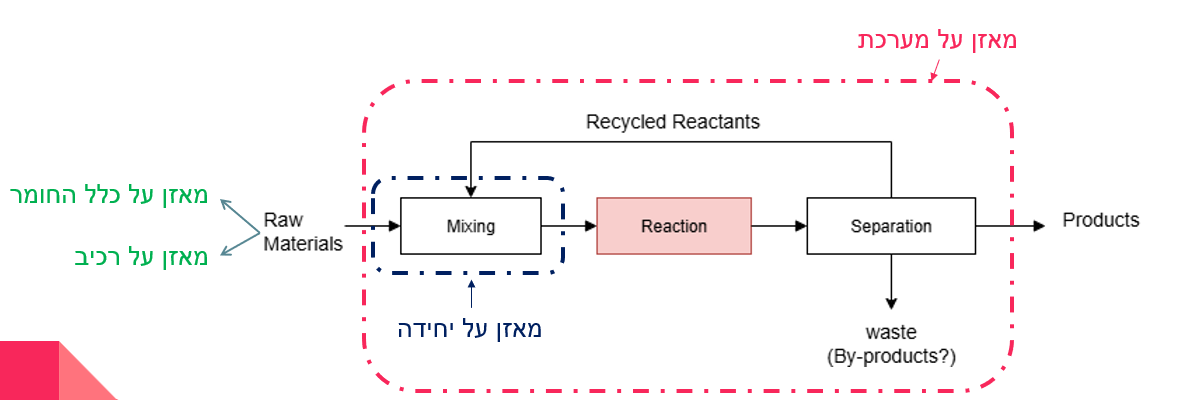
\includegraphics[width=6.5in,height=2.19236in]{images/IntroToCHemEng2/media/image47.png}

}

\caption{- מאזן מסה על מערכת/מאזן מסה על יחידה}

\end{figure}%

\subsection{סוגי תהליכים: מנתי, חצי־מנתי
ורציף}\label{ux5e1ux5d5ux5d2ux5d9-ux5eaux5d4ux5dcux5d9ux5dbux5d9ux5dd-ux5deux5e0ux5eaux5d9-ux5d7ux5e6ux5d9ux5deux5e0ux5eaux5d9-ux5d5ux5e8ux5e6ux5d9ux5e3}

כשאנחנו מדברים על תהליכים אנחנו מחלקים אותם למספר סוגים. התהליך יכול
להיות מנתי, חצי-מנתי או רציף. כמו כן, נוכל לדבר על מערכות במצב עמיד
(steady state, STST) או מערכות העוברות שינוי (transient).

\begin{itemize}
\item
  \textbf{תהליך מנתי, אצווה (batch)}\\
  בתהליך מנתי כל החומר מוכנס למערכת בתחילת התהליך, ואין זרימה פנימה או
  החוצה בזמן הפעולה. לאחר תקופה מסוימת התהליך נעצר, והתוצר נשלף. לדוגמא
  - תהליך התסיסה בהכנת יין הוא מנתי. במאזן המסה מדובר במערכת סגורה
  מבחינת מסה, ולכן משתמשים בדרך כלל במאזן אינטגרלי בין מצב התחלתי לסופי.
\item
  \textbf{תהליך חצי־מנתי (Semi-batch)}\\
  בתהליך חצי מנתי, אנו מתחילים עם מערכת המכילה חלק מהרכיבים, אך יתר
  הרכיבים נכנסים או יוצאים תוך כי כדי התהליך. לדוגמה, ייתכן הזנה מתמדת
  של מגיב חדש, אך בלי זרם מוצרים החוצה עד סוף התגובה. כמו בהכנת מרנג:
  מקציפים חלבונים במיקסר תוך כדי הוספה הדרגתית של סוכר. בתחילת התהליך
  קיימת כמות קבועה של חלבונים, ובמהלך ההקצפה נכנס חומר חדש (סוכר) אל תוך
  המערכת באופן הדרגתי, אך דבר אינו יוצא ממנה עד לסיום התהליך.
\item
  \textbf{תהליך רציף (Continuous):}\\
  בתהליך רציף חומר נכנס ויוצא כל הזמן, והתהליך מתרחש ללא הפסקה. לאחר
  תקופה מסוימת המערכת מגיעה למצב יציב שבו כל הזרמים, ההרכבים והטמפרטורות
  קבועים בזמן - זהו מצב עמיד.
\end{itemize}

{- סוגי תהליכים}

\subsection{סיכום}\label{ux5e1ux5d9ux5dbux5d5ux5dd-7}

\begin{itemize}
\item
  מערכת - חלק מן העולם שאנו תחומים בגבול כדי לבצע עליו מאזן מסה.

  \begin{itemize}
  \item
    הגבול יכול להיות ממשי או דמיוני
  \item
    מה שעובר את הגבול נכנס לחשבון; מה שלא לא. בחירת הגבולות קובעת את
    המאזן.
  \end{itemize}
\item
  סוגי מערכות:

  \begin{itemize}
  \item
    מערכת פתוחה: יש מעבר מסה דרך הגבול.
  \item
    מערכת סגורה: אין מעבר מסה, אבל אנרגיה יכולה לעבור.
  \item
    מערכת מבודדת: לא מסה ולא אנרגיה עוברות.
  \end{itemize}
\item
  במערכות מורכבות אפשר לבחור תתי־מערכות שונות; כל בחירה יוצרת מאזן אחר
  אך עקבי.
\item
  סוגי תהליכים:

  \begin{itemize}
  \item
    תהליך מנתי: כל החומר בפנים מראש, אין זרימה בזמן התהליך.
  \item
    תהליך חצי־מנתי: חלק מהחומר בפנים, חלק מוזרם פנימה או החוצה במהלך
    התהליך.
  \item
    תהליך רציף כניסה ויציאה רציפות. לרוב שואפים למצב עמיד שבו התנאים
    קבועים בזמן.
  \end{itemize}
\end{itemize}

\section{שלבים בניתוח ופתרון
מערכות}\label{ux5e9ux5dcux5d1ux5d9ux5dd-ux5d1ux5e0ux5d9ux5eaux5d5ux5d7-ux5d5ux5e4ux5eaux5e8ux5d5ux5df-ux5deux5e2ux5e8ux5dbux5d5ux5ea}

בניתוח מערכות תהליכיות חשוב לזהות מראש את מאפייני המערכת, משום שהם
קובעים את צורת המאזנים ואת אופן הפתרון. נהוג למיין מערכות לפי שלושה
היבטים מרכזיים.

\begin{itemize}
\item
  \textbf{מבנה התהליך}- האם מדובר במערכת של \emph{יחידה אחת} עם גבול
  מערכת אחד, או \emph{מערכת רב־יחידתית} שבה זרמים עוברים בין כמה יחידות
  עיבוד?
\item
  \textbf{כימיה בתהליך} - האם המערכת פועלת \emph{ללא תגובה כימית}, כך
  שמספר המינים הכימיים קבוע, או שמתרחשת \emph{תגובה כימית} המשנה את הרכב
  המערכת ואת מספר המאזנים הבלתי תלויים.
\item
  \textbf{אופי הפעולה בזמן} - האם התהליך פועל במצב \emph{עמיד} (כל
  המשתנים קבועים בזמן) \emph{מנתי} (עיבוד אצווה ללא זרימה רציפה), או
  \emph{חצי־מנתי} שבו רק חלק מהזרמים רציפים.
\end{itemize}

סיווג ראשוני זה מאפשר לבחור את הכלים המתאימים לניתוח המערכת, ובהמשך
לבנות פתרון עקבי וברור. בשלב ראשון נתחיל עם המערכות הפשוטות ביותר -
מערכות בעלות יחידה אחת וללא תגובה כימית. כדי להדגים את שיטת העבודה נפתח
בשאלה פשוטה מאוד. הפשטות כאן מכוונת: היא מאפשרת לנו להתמקד בשלבי הניתוח
עצמם ולא במורכבות חשבונית. נציג את השאלה במלואה, ולאחר מכן נפתור אותה
בהדרגה, שלב אחר שלב, תוך הדגמה מפורשת של כל רכיב בתהליך הפתרון.

שאלה לדוגמא: לתוך סיר מוסיפים 5.0kg תותים טריים המכילים 90\%wt מים ו-
3.0kg סוכר לבן. מבשלים את הריבה ובסיום הבישול מקבלים 6.0kg ריבה מוכנה.
נניח כי כל הסוכר/מוצקי התותים נשארים בריבה. מהו אחוז המים בריבה המוגמרת
\%wt?

בואו נעקוב אחר פתרון השאלה שלב אחר שלב

\subsection{שלב א: ניתוח והגדרת
הבעיה}\label{ux5e9ux5dcux5d1-ux5d0-ux5e0ux5d9ux5eaux5d5ux5d7-ux5d5ux5d4ux5d2ux5d3ux5e8ux5ea-ux5d4ux5d1ux5e2ux5d9ux5d4}

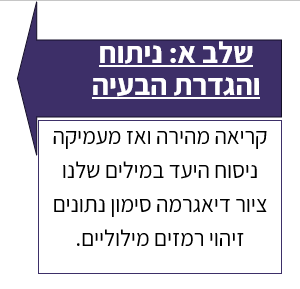
\includegraphics[width=2.08344in,height=1.97927in]{images/IntroToCHemEng2/media/image49.png}

בשלב הראשון עוצרים לרגע עם העיפרון ומתרכזים רק בקריאה מדויקת של השאלה.
המטרה כאן אינה לקפוץ מיד לפתרון, אלא להבין מה בדיוק מבקשים מאיתנו: מה
נתון, מה נדרש, ומהי נקודת הסיום שאליה אנחנו אמורים להגיע. בשלב זה עדיין
אין צורך לזהות את מבנה המערכת או את דרך הפתרון; לעיתים קרובות הקריאה
הראשונית אפילו אינה חושפת את כל מאפייני התהליך, ואלו יתבררו רק בשלבים
הבאים. כאן אנו פשוט מגדירים לעצמנו את מטרת החישוב ואת סוג התוצאה שאנו
מחפשים.

לתוך הסיר נכנסים שני מרכיבים: תותים טריים, שמורכבים ממוצקי תותים ומים,
וסוכר טהור. לאחר הבישול מתקבלת ריבה במשקל ידוע. לפי הנתון, כל המוצקים
וכל הסוכר נשארים בריבה, ולכן השינוי היחיד הוא כמות המים שמתאדה במהלך
הבישול. מטרתנו היא למצוא מהו אחוז המים בריבה הסופית מתוך מסת הריבה
הכוללת.

לאחר מכן מעבירים את המידע מתיאור מילולי לייצוג חזותי מסודר. דיאגרמה טובה
אינה רק ציור סכמטי, אלא כלי לארגון המידע. בשלב זה חשוב לזהות גם את
הנתונים המספריים כולל יחידות, וגם את הנתונים המילוליים, משום שגם תיאור
מילולי עשוי להכיל מידע כמותי שיש לפרש ולהכניס לדיאגרמה. הדיאגרמה תאפשר
לנו לזהות את הזרמים הרלוונטיים ולבחור את גבולות המערכת.

יש כמה כללים מקובלים שמסייעים לשמור על בהירות:

\begin{itemize}
\item
  מקובל לכתוב את הנתון הכולל של כל זרם מעל החץ, ואת פירוט הרכיבים מתחת
  לחץ. כתיבה עקבית כזו מאפשרת לזהות במהירות מהי המסה הכוללת של כל זרם
  ומהו הרכבו.
\item
  אנו מתייחסים לכל המשתנים המשפיעים על המאזן. במקום שבו ערך הנתון ידוע
  לנו, נכתוב אותו במפורש; במקום שבו חסר מידע, נשתמש בנוטציה שמסמנת את
  הנעלם. תיאורטית, ניתן לבחור כל סימון שנוח לנו, אבל עדיף לבחור נוטציה
  מדעית מקובלת ולהתמיד בה לאורך כל הדרך. כתיבה קונסיסטנטית מקלה על זיהוי
  המאזנים הבלתי תלויים ועל מעקב אחר כל מרכיב בתהליך.
\item
  עבור נתונים שאינם ידועים נכתוב גם את היחידות שאנו מעוניינים בהם
\end{itemize}

דיאגרמה שנכתבה היטב משמשת לנו כנקודת מוצא לשלב הבא, שבו נבצע ניתוח של
המשתנים הידועים והנעלמים ונגדיר את המשוואות המתאימות.

לתוך סיר מוסיפים \hl{5.0kg תותים טריים} המכילים \hl{90\%wt מים} ו-
\hl{3.0kg סוכר לבן.} מבשלים את הריבה ובסיום הבישול מקבלים \hl{6.0kg
ריבה} מוכנה. \hl{נניח כי כל הסוכר/מוצקי התותים נשארים בריבה.} מהו אחוז
המים בריבה המוגמרת \%wt?

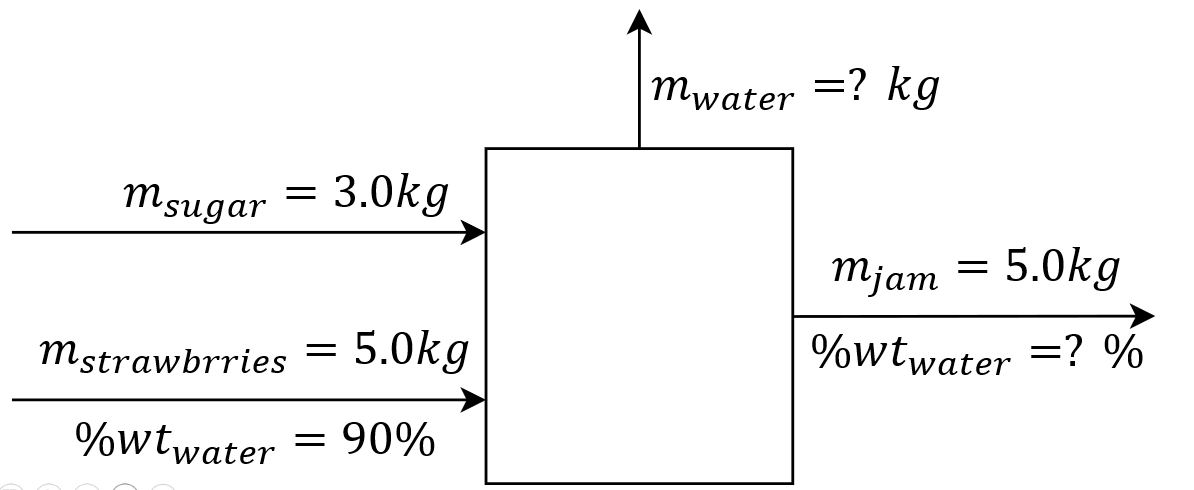
\includegraphics[width=6.5in,height=2.66736in]{images/IntroToCHemEng2/media/image50.png}

\subsection{שלב ב: תכנון
הפתרון}\label{ux5e9ux5dcux5d1-ux5d1-ux5eaux5dbux5e0ux5d5ux5df-ux5d4ux5e4ux5eaux5e8ux5d5ux5df}

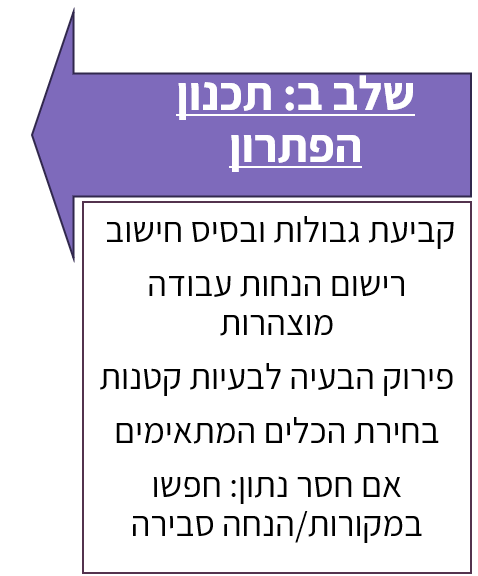
\includegraphics[width=1.78127in,height=2.14647in]{images/IntroToCHemEng2/media/image51.png}

\ul{קביעת גבולות}

איך נבחר את גבול המערכת? לאחר ציור הדיאגרמה נבחר את המערכת שאותה ננתח על
ידי הגדרת הגבולות שלה. הגבול צריך לכלול בדיוק את החלק בתהליך שבו מתרחש
השינוי הרלוונטי לחישוב. כדי לבחור גבול מתאים נשאל?

\begin{itemize}
\item
  מה אני מנסה לחשב? המערכת חייבת לכלול את כל מה שמשפיע על הגודל הזה
\item
  אילו זרמים נכנסים ויוצאים מהמערכת? המערכת צריכה לכלול את כל מה שמשפיע
  על הגודל הזה.
\item
  האם המאזן על המערכת הזו נותן מספיק מידע? אם לא יש להגדיר מערכות נוספות
\end{itemize}

לעיתים גבול אחד אינו נותן את כל המשוואות או אינו מבודד את המשתנים
הדרושים. במקרים כאלה נגדיר מגדירים מערכת נוספת עם גבול שונה (רחב או צר
יותר), נכתוב מאזן חדש עבור המערכת הזו ונשלב בין כל המאזנים שהתקבלו. על
תהליך זה ניתן לחזור גם פעם שלישית, רביעית ואף יותר, כתלות במורכבות
המערכת, עד שהמידע הדרוש לפתרון יהיה מלא וברור. חשוב לוודא שהמערכות
שהגדרנו באמת מספקות מידע בלתי תלוי זו מזו, נדבר על זה בהרחבה כשנגיע
לניתוח דרגות חופש.

יש לנו רק יחידה אחת ולכן גבולות המערכת יהיו גבולות היחידה

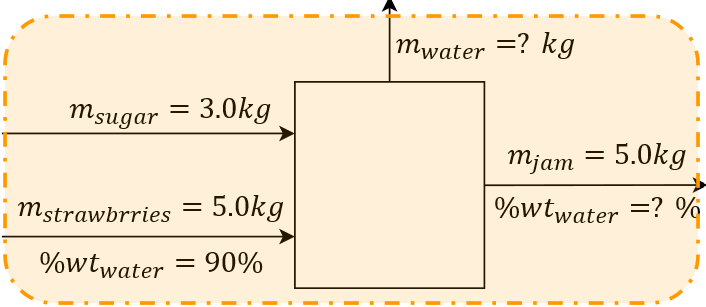
\includegraphics[width=4.90303in,height=2.13205in]{images/IntroToCHemEng2/media/image52.png}

\ul{בחירת בסיס חישוב}

בכל בעיית מאזני מסה נדרש לבחור \textbf{בסיס חישוב}, כמות או קצב זרימה של
אחד הזרמים או אחד ממרכיבי הזרם שבתהליך, שעל פיו נבנה את כל החישובים.
הבחירה בבסיס אינה קובעת את הפתרון הפיזי של הבעיה, אלא רק יוצרת מערכת
נוחה ומסודרת של משוואות. כאשר נתונים קצבי זרימה או כמויות בשאלה, לרוב
נבחר את אחד מהם כבסיס טבעי. אם אין נתון כזה, מקובל להניח ערך נוח,
בדרך-כלל לזרם בעל הרכב ידוע. למשל, כאשר ההרכב ניתן כשברים משקליים נוח
לבחור בסיס של 100kg וכאשר ההרכב ניתן כשברים מולריים, נבחר בדרך כלל בסיס
של 100mol. בחירה קונסיסטנטית של בסיס מאפשרת לכתוב מאזנים ברורים, לקבוע
את הנעלמים, ולפתור את מערכת המשוואות בצורה נשלטת ומסודרת.

במקרה הזה, סביר להניח שמה שהכתיב לנו את כמות הריבה שאנחנו מכינים זה כמות
התותים שהיה לנו, ולכן נבחר את זה כבסיס חישוב.

\ul{רישום הנחות}

במצבים רבים המערכת האמיתית מורכבת בהרבה מכפי שאפשר לייצג בחישוב ידני.
מטרתן של הנחות העבודה היא לפשט את המודל כך שיהיה ניתן לנסח עבורו מאזנים
ברורים ולפתור אותם. הנחות אינן "קיצור דרך" אלא כלי שמאפשר לנו לוותר
באופן מבוקר על פרטים שאינם חיוניים לחישוב, כדי ליצור גרסה נקייה ופשוטה
יותר של התהליך - גרסה שאותה כן ניתן לנתח באופן ישיר. עם זאת, הנחה טובה
חייבת לעמוד בשני מבחנים חשובים.

\textbf{המבחן הראשון הוא מבחן ההיגיון הפיזיקלי.}\\
הנייר סופג הכל, אבל התהליך הפיזיקלי לא. מותר לפשט, אך הפישוט חייב להיות
עקבי עם המציאות. למשל, במרבית התמיסות המדוללות ניתן להניח שהצפיפות דומה
לזו של מים; אך זה אינו סביר עבור מי מלח רוויים מים המלח. כל הנחה חייבת
להתאים להרכב החומרים, לאופי היחידה התהליכית ולחוקי השימור הבסיסיים.

\textbf{המבחן השני הוא בדיקה בדיעבד.}\\
הנחות הן זמניות במהותן: אנחנו בוחרים אותן כדי להתחיל את החישוב, אבל
חייבים לבדוק שהמודל הפשוט שבנינו אכן תואם את התוצאות. ייתכן שנאסוף
נתונים ונגלה שההנחה שלנו (``רק מים מתאדים'', למשל) לא עומדת בחינה - ואז
נידרש לשוב ולבנות מודל מעודכן. זהו חלק טבעי מתהליך בניית מודלים: ניסוח,
בדיקה, התאמה מחדש.

חשוב להבדיל בין שלושה סוגי מידע שונים

\begin{itemize}
\item
  \textbf{נתונים (Data)}\\
  אלו ערכים שניתנים במפורש בשאלה: מספרים, הרכבים, קצבי זרימה, ערכים
  ועקרונות פיזיקליים חד-משמעיים. הנתונים הם העובדות היחידות שאיננו מרשים
  לעצמנו לשנות או לפרש מחדש. הם מהווים את בסיס החישוב.
\item
  \textbf{הנחות שניתנו לנו בשאלה}\\
  אלו קירובים שנאמר לנו באופן מפורש שמותר לנו להניח בשאלה. משפטים כאלה
  מתפקדים עבורינו כנתונים לכל דבר, אבל הם מגלמים בתוכם הפשטה של המודל.
  הם מכתיבים לנו אילו תהליכים אנחנו אמורים לכלול ואילו להתעלם מהם.
\item
  \textbf{הנחות שאנחנו מוסיפים בעצמנו}\\
  כאן נכנס שיקול הדעת שלנו: אלו הנחות שאינן מופיעות בשאלה אבל נדרשות כדי
  לפשט את המודל או להשלים מידע חסר. ההנחות הללו חייבות להיות פיזיקליות
  והגיוניות והן חייבות להיבדק בדיעבד.\\
  זוהי ה''אמנות'' של ניתוח תהליכים: להניח מספיק כדי שהבעיה תהיה פתירה
  ותיתן לנו תוצאה בקירוב טוב, אבל לא להניח יותר מדי כך שהשגיאה תהיה
  גדולה מדי או להניח דברים שסותרים את התהליך.
\end{itemize}

הנחות מתוך השאלה\\
- "כל הסוכר/מוצקי התותים נשארים בריבה"\\
- מכאן נובע באופן ישיר שהחומר היחיד שיוצא לא כחלק מהריבה הוא מים

הנחות שאנחנו מוסיפים\\
- גבולות המערכת קשיחים, אין אובדן של חומר (נניח עקב התזה או דליפה)\\
-אין שחרור של גזים נוספים (למשל שחרור של פחמן דו חמצני עקב שריפת סוכרים)

\ul{פירוק הבעיה לבעיות קטנות}

פירוק בעיה לבעיות קטנות הוא לא שלב שנעשה ב״מכה אחת״. ברוב המקרים מתחילים
עם חלוקה ראשונית של הצעדים, ואז מגלים באמצע הדרך שחסר נתון, שהסדר לא
עובד, או שצריך לחשב משהו מוקדם יותר ממה שחשבנו. זה טבעי לחלוטין: פירוק
טוב כמעט תמיד מתפתח באופן איטרטיבי. מנסים סדר אחד, בודקים מה אפשר לחשב
כבר עכשיו, מה עדיין חסום, ומה דורש שלב נוסף. אם משהו לא מסתדר - מחליפים
סדר או מוסיפים תת־בעיות.

לא חייבים לחשוב על התהליך באופן לינארי מההתחלה עד הסוף. לפעמים נתחיל
מהשלבים הראשונים של התהליך, לפעמים דווקא מהתוצאה הסופית שאליה אנחנו
רוצים להגיע, ולפעמים נזהה צוואר בקבוק - שלב מסוים שבו מרוכזת עיקר
המורכבות - ונבנה את החלוקה לבעיות קטנות סביבו. המטרה אינה למצוא את
הפירוק המושלם בניסיון הראשון, אלא לבנות בהדרגה מסלול עבודה שכל שלב בו
מסתמך על מידע שכבר נמצא בידינו. עם הזמן (והנסיון) לומדים לזהות מראש
פירוקים יעילים יותר ופחות כך שהתהליך מתקצר.

חלוקה לבעיות קטנות - כמה מים הכנסנו למערכת?\\
- כמה מים התאדו?\\
- כמה מים נשארו בריבה?

\ul{בחירת הכלים המתאימים ומציאת נתונים נוספים}

לאחר שהוגדרו המערכת, הגבולות וההנחות, מגיע השלב שבו בוחרים את הכלים
שיאפשרו להתקדם בפועל בחישוב. הכלים המרכזיים העומדים לרשותנו הם יחסית
מעטים, אך כמעט כל בעיה במאזני מסה נפתרת באמצעות שילוב ביניהם. ראשית,
נעזרים בהרכבים - שברים משקליים או מולריים - שמאפשרים לתרגם נתונים
מילוליים או יחסיים למסות ומולים של כל רכיב. לצד זאת פועלים חוקי השימור
הבסיסיים, שימור מסה, שימור רכיב מסויים ובהמשך גם שימור אטומים ושימור
אנרגיה. חוקי השימור הם הבסיס לכל מאזן.

כאשר נדרש נתון שאינו מופיע במפורש בשאלה, אפשר להיעזר במשוואות פיזיקליות
כלליות, כמו משוואת הגז האידיאלי, יחסי מסיסות, או קשרים בין נפח, מסה
וצפיפות. במקרים רבים נזדקק גם לנתונים מספרי־נתונים חיצוניים - מסות
מולריות, צפיפויות, מסיסויות, או קבועים תרמודינמיים. לעיתים הנתון הדרוש
קיים, אך ביחידות שאינן מתאימות למאזן, במקרה כזה המרת יחידות פשוטה מאפשרת
להתקדם. ולבסוף, כאשר חסר נתון ואין משוואה פיזיקלית שיכולה לספק אותו,
משלימים את הפער באמצעות הנחה סבירה ועקבית שניתן לבדוק בדיעבד. את כל
הנתונים, המשוואות, ההמרות וההנחות מאחדים בסופו של דבר לכדי מערכת
משוואות, שהן החוליה האחרונה בתהליך הבחירה והחישוב.

נוכל להשתמש בהרכב כדי לחשב את מסת המים בהתחלה, במאזני מסה (כללי+מאזן על
המים) לבדוק איך הם מתחלקים בין הזרמים, ואז בהכרב שוב כדי למצוא את החלק
היחסי של המים

אחר שמגדירים את המערכת, בוחרים את הכלים ומפרקים את הבעיה לצעדים, מגיע
שלב הפתרון עצמו. בשלב זה מתחילים ברישום מסודר של המשוואות בסימנים, תוך
הקפדה שהן יהיו \textbf{הומוגניות ביחידות} - כלומר שכל איבר בכל משוואה
יופיע באותן יחידות פיזיקליות. לאחר מכן מציבים את הערכים הידועים בצורה
מסודרת, ומשאירים רק את הנעלמים הדרושים לפתרון. את הפתרון ניתן לבצע בשלוש
דרכים: אלגברית (כאשר קיימת משוואה סגורה וברורה), נומרית (כאשר נדרש חישוב
חוזר או פתרון משוואות שאינן לינאריות), או גרפית (כאשר היחסים המתקבלים
נתונים כעקומות או כטבלאות).

העבודה בשלב זה לעיתים איטרטיבית: אם הפתרון אינו עקבי, התוצאה אינה
הגיונית, או שהיחידות אינן מתאימות - חוזרים צעד אחד אחורה ומעדכנים
משוואה, נתון או הנחה. בסיום, מציגים את התוצאות בצורה נקייה, תוך שימוש
ב\textbf{דיוק הנדסי סביר} - לא יותר ספרות ממה שמצדיקים הנתונים ולא פחות
ממה שנדרש כדי להעביר את המשמעות הכמותית של הפתרון.

\subsection{\texorpdfstring{\emph{שלב ג: הפתרון
עצמו}}{שלב ג: הפתרון עצמו}}\label{ux5e9ux5dcux5d1-ux5d2-ux5d4ux5e4ux5eaux5e8ux5d5ux5df-ux5e2ux5e6ux5deux5d5}

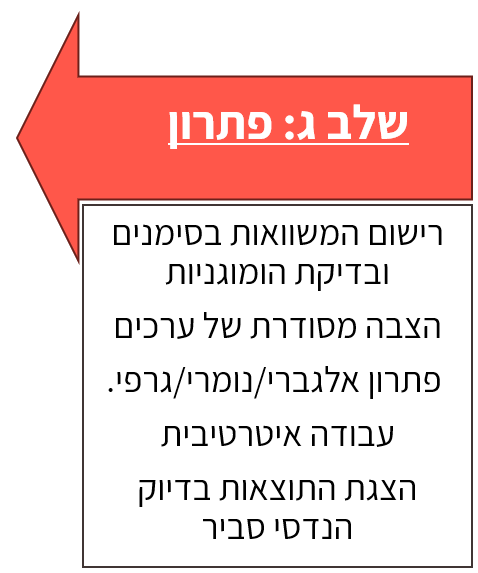
\includegraphics[width=1.76125in,height=2.11128in]{images/IntroToCHemEng2/media/image53.png}

לאחר שמגדירים את המערכת, בוחרים את הכלים ומפרקים את הבעיה לצעדים, מגיע
שלב הפתרון עצמו. בשלב זה נתחיל ברישום מסודר של המשוואות בסימנים, תוך
הקפדה שהן יהיו \textbf{הומוגניות ביחידות}, כלומר שכל איבר בכל משוואה
יופיע באותן יחידות פיזיקליות. לאחר מכן מציבים את הערכים הידועים בצורה
מסודרת, ומשאירים רק את הנעלמים הדרושים לפתרון. בשלב זה לרוב נפתור את
המשוואות באופן אלגברי, ז"א באופן מתמטי ישיר. בהמשך הדרך אנו נקבל משוואות
שלא ניתן לפתור באופן מתמטי ישיר, ונוכל רק להעריך את הפתרונות בצורה
נומרית או גרפית.

\textbf{פתרון אלגברי:} מציאת הנעלם על ידי סידור המשוואות ופתרון מפורש
באמצעות פעולות אלגבריות רגילות.\\
\textbf{פתרון נומרי:} מציאת ערך מקורב לנעלם באמצעות חישוב חוזר או שיטת
קירוב, כאשר אין פתרון מפורש.\\
\textbf{פתרון גרפי:} קביעת ערך הנעלם מתוך גרף או טבלה, בדרך כלל לפי
נקודת חיתוך או ערך מתאים על עקומה.

העבודה בשלב זה לעיתים איטרטיבית: אם הפתרון אינו עקבי, התוצאה אינה
הגיונית, או שהיחידות אינן מתאימות: חוזרים צעד אחד אחורה ומעדכנים משוואה,
נתון או הנחה. בסיום, מציגים את התוצאות בצורה נקייה תוך שימוש בדיוק הנדסי
סביר, לא יותר ספרות ממה שמצדיקים הנתונים ולא פחות ממה שנדרש כדי להעביר
את המשמעות הכמותית של הפתרון.

מסת המים בכניסה

\[5.0kgStrawberries*\frac{90kgWater}{100kgStrawberries} = 4.5kgWaterInStraberries\]

מאזן מסה כללי

\[m_{sugar} + m_{strawberries} = m_{jam} + m_{water}\]

מאזן מסה על המים

\[m_{WaterInStrawbwrries} = m_{water} + m_{WaterInJam}\]

מאזן מסה כללי

\[3.0kg + 5.0kg = 6.0kg + m_{water}\]

\[m_{water} = 2.0kg\]

מאזן מסה על המים

\[4.5kg = 2.0kg + m_{WaterInJam}\]

\[m_{WaterInJam} = 2.5kg\]

מציאת האחוז המסתי של מים בריבה

\[\% wt = \frac{m_{WaterInJam}}{m_{jam}}*100\%\]

\[\% wt = \frac{2.5kg}{6.0kg}*100\% = 41.66666\% = 42\%\]

\emph{מסת המים מהווה 42\% ממסת הריבה}

\subsection{שלב ד בדיקה
ואימות}\label{ux5e9ux5dcux5d1-ux5d3-ux5d1ux5d3ux5d9ux5e7ux5d4-ux5d5ux5d0ux5d9ux5deux5d5ux5ea}

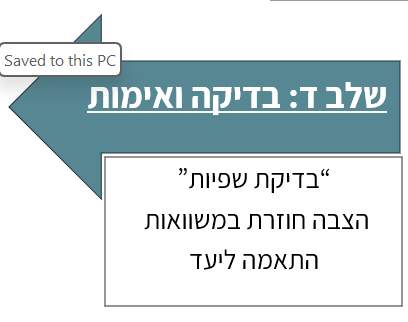
\includegraphics[width=2.00079in,height=1.5153in]{images/IntroToCHemEng2/media/image54.png}

לאחר שמתקבלת התוצאה המספרית, יש לבצע בדיקה סופית שמוודאת שהפתרון אכן
תואם את התהליך הפיזיקלי ואת כל מה שהוגדר בשלבי העבודה הקודמים. בשלב זה
בודקים את ``שפיות'' התוצאה: האם היא בטווח הגיוני? האם היא עומדת בכל
ההנחות? האם היחידות עקביות? לאחר מכן מבצעים הצבה חוזרת של התוצאה
במשוואות המקוריות כדי לוודא שהמאזן נסגר במדויק, ושאין סתירה בין שלבי
החישוב. אם משהו אינו מסתדר - חוזרים שלב אחד אחורה, מתקנים ומאמתים שוב.
המטרה היא לוודא שהתוצאה אינה רק חישובית נכונה, אלא גם פיזיקלית סבירה
ומתאימה לייעד שאליו כיוונו.

קיבלנו 42\% וזהו ערך הגיוני. אם היינו מקבלים ערך שלילי או ערך שגדול
מ100\% היינו צריכים לבדוק את עצמינו. כעת מומלץ (מהתוצאה הסופית, לכמות
המים בריבה, לכמות המים שהתאדתה) כדי לבדוק שהמספרים עדיין מסתדרים. שימו
לב שכתיבה של 41.66666\% אינה מדוייקת מבחינה פיסיקלית. רקמת הדיוק של
המדידה שלנו לא מספיק טובה. באופן כללי ניתן להגיד שיש לנו שתי ספרות
משמעותיות. ובאופן מחמיר נגיד שיש לנו ספר משמעותית אחת (בגלל הנתון של
אחוז המים בתותים, 90\% זו ספרה משמעותית אחת) כך שהמחמירים יגידו שיש 40\%
מים בריבה, ושאין לנו אפשרות לחשב במדויק יותר.

\subsection{חישוב מאזני מסה בסיסיים (ללא תגובה
כימית)}\label{ux5d7ux5d9ux5e9ux5d5ux5d1-ux5deux5d0ux5d6ux5e0ux5d9-ux5deux5e1ux5d4-ux5d1ux5e1ux5d9ux5e1ux5d9ux5d9ux5dd-ux5dcux5dcux5d0-ux5eaux5d2ux5d5ux5d1ux5d4-ux5dbux5d9ux5deux5d9ux5ea}

תזכורת - שלבי הפתרון של שאלה בהנדסת תהליך

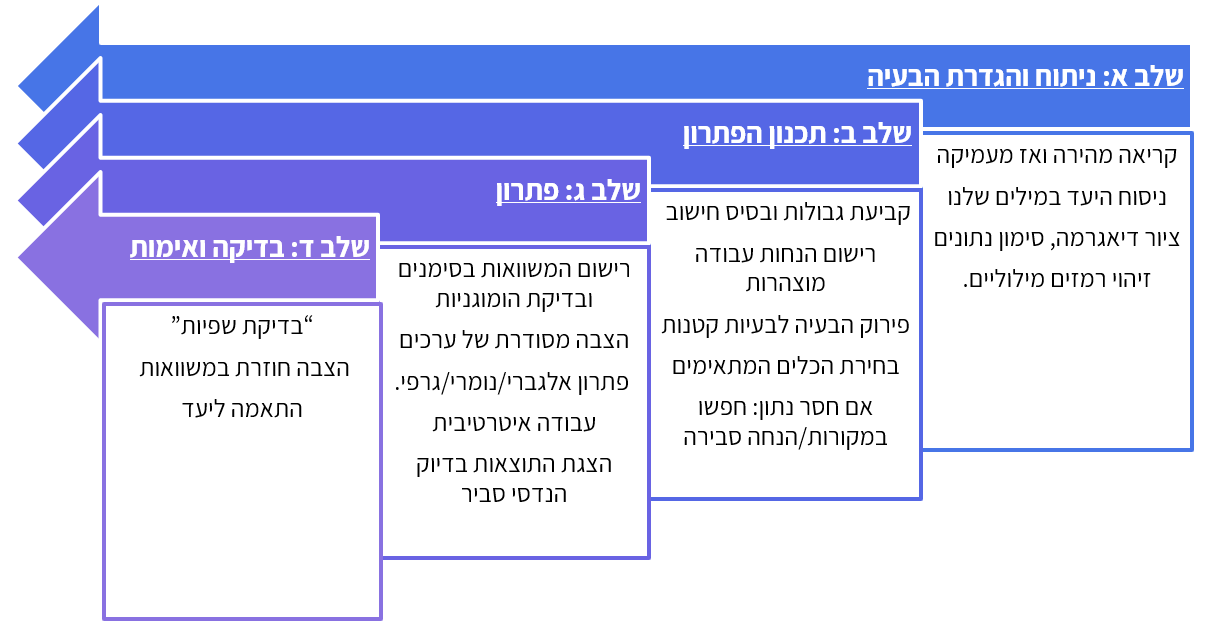
\includegraphics[width=6.5in,height=3.36667in]{images/IntroToCHemEng2/media/image55.png}

\subsubsection{מאזן חומר על מצב
עמיד}\label{ux5deux5d0ux5d6ux5df-ux5d7ux5d5ux5deux5e8-ux5e2ux5dc-ux5deux5e6ux5d1-ux5e2ux5deux5d9ux5d3}

במפעל לייצור אתנול ביולוגי פועל עמוד זיקוק רציף. על מנת לעמוד בדרישות
האיכות של הדלק, עלינו לזקק אותו עד לרמה של 90\% אתנול. המערכת מוזנת
בתמיסת 40\% אתנול בהזנה של \(1000\frac{Kg}{h}\), הזרם התחתון הודגם
והתגלה כי ריכוז האתנול בו הוא 5\%. המערכת במצב יציב ואין צבירה של חומר
בעמוד. מה יהיו הספיקות בזרמי היציאה? כל האחוזים בשאלה הם אחוזים מסתיים.
זהו תהליך זיקוק שמטרתו להגיע לריכוז אתנול גבוה. אנו יודעים את הנתונים
בכניסה, ואנחנו יודעים מה הריכוזים ביציאה. המטרה למצוא את הספיקות ביציאה.
כמה ק"ג לשעה יש בכל אחד מהזרמים?
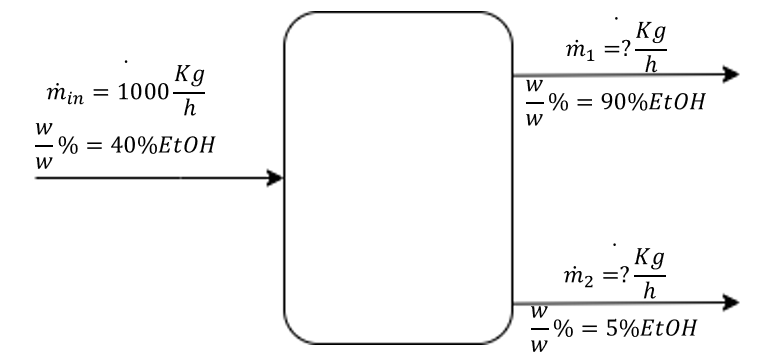
\includegraphics[width=5.29194in,height=2.48624in]{images/IntroToCHemEng2/media/image56.png}
למען הנוחות, נעביר את האחוזים המסתיים הנתונים לצורה מפורשת
\[\frac{w}{w}\% = 40\% EtOH = \frac{40kgEtOH}{100kgSolution}\]
\[\frac{w}{w}\% = 90\% EtOH = \frac{90kgEtOH}{100kgSolution}\]
\[\frac{w}{w}\% = 5\% EtOH = \frac{50kgEtOH}{100kgSolution}\]

נתון כי המערכת במצב עמיד,\\
נכתוב מאזני מסה על המערכת כולה, ועל האתנול בלבד

\emph{מאזן מסה כללי} \({\dot{m}}_{in} = \dot{m_{1}} + {\dot{m}}_{2}\)

\emph{מאזן על האתנול}
\({\dot{m}}_{in}\frac{w}{w}_{in} = \dot{m_{1}}\frac{w}{w}_{1} + {\dot{m}}_{2}{\frac{w}{w}_{in}}_{2}\)

\emph{נציב:\\
מאזן מסה כללי} \(1000\frac{Kg}{h} = \dot{m_{1}} + {\dot{m}}_{2}\)

\emph{מאזן על האתנול}

\[1000\frac{Kg_{solution}}{h}*\frac{40KgEtOH}{100Kg_{solution}} = \dot{m_{1}}\frac{90KgEtOH}{100Kg_{solution}} + {\dot{m}}_{2}\frac{5KgEtOH}{100Kg_{solution}}\]

קיבלנו שתי משוואות בשני נעלמים, מכאן ואילך זה פיתוח אריתמתי (העברת
אגפים, הכפלה בקבועים וכדומה) שבסופו נקבל

\[\dot{m_{1}} = 410\frac{Kg}{h},\dot{m_{2}} = 590\frac{Kg}{h}\]

כדי לוודא שהתשובות נכונות נציב אותן בחזרה במשוואות ונבדוק אם המשוואות
מתקיימות

\emph{מאזן מסה
כללי}\(1000\frac{Kg}{h} = 410\frac{Kg}{h} + 590\frac{Kg}{h}\)

\emph{מאזן על האתנול}

\[1000\frac{Kg_{solution}}{h}*\frac{40KgEtOH}{100Kg_{solution}} = 410\frac{Kg}{h}\frac{90KgEtOH}{100Kg_{solution}} + 590\frac{Kg}{h}\frac{5KgEtOH}{100Kg_{solution}}\]

\subsubsection{מאזן חומר על תהליך
מנתי}\label{ux5deux5d0ux5d6ux5df-ux5d7ux5d5ux5deux5e8-ux5e2ux5dc-ux5eaux5d4ux5dcux5d9ux5da-ux5deux5e0ux5eaux5d9}

הסטודנטית החרוצה סתוונית נדרשת להכין מנה (Batch) של 1,000 ליטר תמיסת מלח
פיזיולוגית (Saline) בריכוז של 0.9\% משקלי. לרשותה עומדים שני מקורות:

תמיסת מלח מרוכזת בריכוז 5.0\% (w/w).

תמיסת מלח מדוללת בריכוז 0.50\% (w/w).

כמה קילוגרמים של כל אחת מהתמיסות יש להזין למיכל הערבוב כדי לקבל את המנה
המבוקשת?\\
ניתן להניח כי צפיפות תמיסת המלח הפזיולוגית שווה לצפיפות מים.

\textbf{פתרון:}

אנחנו צריכים לערבב את שתי התמיסות על מנת לקבל 1000 ליטר של תמיסת מלח
בריכוז מסויים. אנחנו צריכים לגלות מהי המסה הנדרשת לערבב מכל תמיסה כדי
לקבל את הריכוז ונפח הרצויים.

דיאגרמה ונתונים -\\
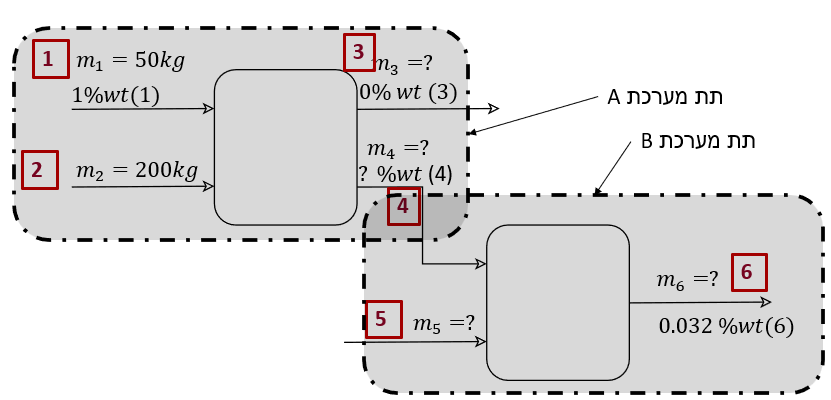
\includegraphics[width=6.28623in,height=2.33465in]{images/IntroToCHemEng2/media/image57.png}

אנו יכולים להניח שצפיפות התמיסה המתקבלת היא כצפיפות המים. נוכל לחשב את
מסת התמיסה המתקבלת ואז נבצע שני מאזני מסה -- מאזן כולל ומאזן על רכיב

\emph{מסת התמיסה בסוף התהליך}

\[m_{f} = 1000L*\frac{m^{3}}{1000L}*\frac{1000kg}{m^{3}} = 1000kg\]

\emph{מאזן מסה כולל}

\[m_{1} + m_{2} = m_{f}\]

*מאזן מסה על המלח (מטעמי נוחות עברתי לשברים מסתיים במקום אחוזים)*
\[m_{1}*0.05 + m_{2}*0.005 = 1000kg*0.009\]

\[0.05m_{1} + 0.005\left( 1000kg - m_{1} \right) = 9kg\]

\[0.05m_{1} + 5kg - 0.005m_{1} = 9kg\]

\[0.05m_{1} + 5kg - 0.005m_{1} = 9kg\]

\[0.045m_{1} = 4k\]

\[m1 = 88kg = 90kg\]

\[m_{2} = 1000kg - 90kg = 910kg\]

צריך יותר מהתמיסה השנייה כי הריכוז יותר קרוב לריכוז של התמיסה השנייה.\\
אם רוצים להיות בטוחים שלא היתה טעות חישוב, ניתן לעשות את החישוב פעם
שנייה אך עם הצבה הפוכה
\(0.05\left( 1000 - m_{2} \right) + 0.005m_{2} = 9kg\)

\subsubsection{מאזן חומר על תהליך חצי
מנתי}\label{ux5deux5d0ux5d6ux5df-ux5d7ux5d5ux5deux5e8-ux5e2ux5dc-ux5eaux5d4ux5dcux5d9ux5da-ux5d7ux5e6ux5d9-ux5deux5e0ux5eaux5d9}

במפעל משקאות קלים נעשה שימוש במיכלי נירוסטה גדולים לצורך מילוי והכנת
משקאות מוגזים. לפני שממלאים משקה למיכל יש להבטיח שרמת החמצן החופשי במיכל
נמוכה, כדי למנוע חמצון של המשקה ושינויים בטעם או בצבע. לאחר שהמיכל
מתרוקן, החלל הפנוי שבו מתמלא שוב באוויר מהסביבה, ולכן נותר בו חמצן שיש
לסלק לפני מילוי המשקה. לשם הורדת כמות החמצן מבצעים תהליך Purging:
מזרימים לתוך המיכל גז פחמן דו-חמצני \(CO_{2}\) טהור, אשר נכנס מתחתית
המיכל ודוחף החוצה תערובת של אוויר ו-\(CO_{2}\) מהפתח העליון.

ידוע כי בתחילת התהליך יש במיכל \(\ m_{O_{2},i} = 32g\ \)חמצן חופשי.
מערכת ה־Purging מסירה חמצן בקצב קבוע של \(r = 0.8\text{~g/min}\). גז
ה-CO₂ הנכנס אינו מכיל חמצן. אין תגובה כימית היוצרת או צורכת חמצן. הטכנאי
הפעיל את מערכת הpurging במשך עשרים דקות. כמה חמצן ישאר במיכל בסוף
התהליך?\\
\strut \\
פתרון:\\
ניסוח במילים שלנו: בתוך המיכל יש חמצן, מוציאים אותו על ידי הזרמת פחמן דו
חמצני שדוחף את החמצן החוצה בקצב קבוע. כמה חמצן נשאר בכלי אחרי 20 דקות?

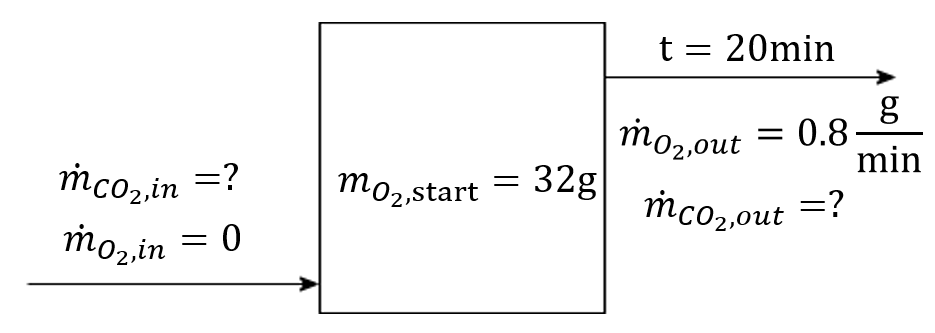
\includegraphics[width=4.58862in,height=1.63396in]{images/IntroToCHemEng2/media/image58.png}

נראה כאילו חסר לנו הרבה מידע, אבל האמת היא שהפחמן הדו חמצני לא מעניין
אותנו. ברור לנו שיש כמות שנכנסת, כמות שמצטברת בפנים והשאר יוצא, אבל
המספרים לא רלוונטיים כי לא עליהם שאלו אותנו. יספיק לנו מאזן מסה על
החמצן.

מה שהיה בהתחלה פחות מה שיצא נותן לנו את מה שנשאר
\(m_{start} - m_{out} = m_{finish}\)

אנחנו יכולים לחשב כמה יצא לפי הזמן
\(m_{out} = {\dot{m}}_{O_{2},out}*t = 0.8\frac{g}{\min}*20min = 16g\)

ולכן כמות החמצן בסיום תהיה \(32g - 16g = 16g\)

\emph{אנו רואים שהמספר שקיבלנו הוא בטווח הנכון.}

אנקדוטה -- בפעם הראשונה שחישבתי את זה יצא לי שכמות החמצן שיצאה היא 160
גרם, מה שכמובן לא הגיוני, ואז בדקתי וראיתי שהעתקתי נתון לא נכון -- קצב
היציאה היה 0.8g/min ולא 8g/min. אלו בדיוק סוג הטעויות שאנחנו מקווים
למצוא בשלב הזה.

\subsection{\texorpdfstring{ניתוח דרגות חופש \textbf{(}Degrees of
Freedom
Analysis\textbf{)}}{ניתוח דרגות חופש (Degrees of Freedom Analysis)}}\label{ux5e0ux5d9ux5eaux5d5ux5d7-ux5d3ux5e8ux5d2ux5d5ux5ea-ux5d7ux5d5ux5e4ux5e9-degrees-of-freedom-analysis}

.לפני שאנחנו רצים למחשבון ומתחילים להציב מספרים, ישנה שאלה אחת חשובה
שחייבת להישאל:~\textbf{האם הבעיה הזו בכלל ניתנת לפתרון?}

נדמיין שקיבלנו את המשוואה הבאה:\(x + y = 10\). האם ניתן למצוא למשוואה
פתרון יחיד? התשובה היא לא יש לנו שני נעמים, ועבור כל x שנציב נוכל למצוא
y שמתאים לו. למשל עבור x=5 נקבל y=5, ועבור x=-2 נקבל y=12. יש לנו אינסוף
פתרונות אפשריים. כדי לפתור את הבעיה, אנחנו צריכים מידע נוסף. למשל,
משוואה נוספת: \(x - y = 2\). כעת יש לנו שתי משוואות בלתי תלויות ושני
נעלמים -- אנחנו מקבלים פתרון יחיד \(x = 6,\ y = 4\)

בהנדסת תהליכים המצבים מורכבים הרבה יותר, עם עשרות זרמים, רכיבים
ונעלמים.~\textbf{ניתוח דרגות חופש (DOF)}~הוא שיטה שיטתית וקריטית שנועדה
לוודא שיש לנו מספיק מידע כדי לפתור את הבעיה,~\emph{לפני}~שנבזבז זמן יקר
על חישובי סרק או ניסיונות לפתור בעיה שאינה מוגדרת היטב.

מספר דרגות החופש מוגדר כהפרש בין מספר הנעלמים במערכת לבין מספר המשוואות
הבלתי תלויות המקשרות בינהם

\[n_{DOF} = n_{unknowns\_ variables} - n_{indep.\ eq,}\]

כאשר: \(n_{unknown\_ variables}\) - מספר המשתנים הלא ידועים בבעיה
(ספיקות, הרכבים וכו...)\\
ו- \(n_{indep.\ eq,}\) - מספר המשוואות \textbf{\ul{הבלתי-תלויות}}

מתוך \(n_{DOF}\) אנו יכולים להסיק האם ניתן להגיע למסקנה יחידה עבור מערכת
מסויימת.

אם \(n_{DOF} = 0\) נאמר שהבעיה מוגדרת היטב (Well-specified). מאחר ומספר
הנעלמים שווה למספר המשוואות נקבל פתרון יחיד לבעיה.

אם \(n_{DOF} < 0\) נאמר שהבעיה היא יתר-מוגדרת (Over-specified) -- יש
יותר משוואות מנעלמים. במקרה זה יש לנו "יותר מדי מידע". ייתכן שחלק
מהנתונים הם מיותרים (Redundent), אך הסכנה הגדולה יותר היא שנקבל נתונים
הסותרים זה את זה. לדוגמא שעל פי חישוב אחד המערכת נמצאת
בטמפ\textquotesingle{} של 273K, ועל פי חישוב אחר נקבל דווקא 298K. אין
טעם לבזבז טעם בלנסות ולפתור מערכת יתר-מוגדרת אשר ייתכן שמכילה נתונים
סותרים. לכן חשוב מאוד לבדוק את עקביות הנתונים, לוותר על משוואות שלא
נותנות מידע חדש או להסיר אילוצים מיותרים, לדוגמא -- הנחות שהוספנו כדי
לפשט את המערכת.

אם \(n_{DOF} > 0\) נאמר שהבעיה תת-מוגדרת (Underspecified), יש יותר
נעלמים ממשוואות. במקרה זה מבחינה מתמטית יהיו לנו אינסוף פתרונות בדיוק
כמו בדוגמא למעלה. לכן עלינו קודם כל אם זה באמת המצב: אולי פספסנו נתונים
(מספריים או מילוליים)? אולי יש משוואות פיסיקליות נוספות שמשפיעות לנו על
המערכת כמו משוואת הגזים האידיאליים? אולי יש קבועים אותם ניתן להוציא
מהספרות? המשמעות המעשית תלויה בהקשר שבו אנו פועלים:

\begin{itemize}
\item
  \textbf{בחיים האמיתיים (תכנון הנדסי):} דרגות החופש מייצגות
  \textbf{בחירה.} אם קיבלנו \(n_{DOF} = 2\) המשמעות היא שעלינו, כמהנדסים
  ומהנדסות, לקבל החלטה ולקבוע באופן יזום את ערכם של שני משתנים (למשל,
  לקבוע את ספיקת ההזנה ואת טמפרטורת הריאקטור). אלו נקראים "משתני תכנון"
  (Design Variables). ברגע שנקבע את הערכים הללו, שאר המשתנים במערכת
  ייקבעו באופן אוטומטי כתוצאה מכך, והמערכת תהפוך למוגדרת היטב
  \(n_{DOF} = 0\).
\item
  \textbf{במסגרת הקורס (פתרון תרגילים):} בדרך כלל אנו מחפשים פתרון יחיד
  וספציפי. לכן, אם קיבלנו ערך חיובי סביר להניח שחסר לנו מידע -- נתון,
  משוואה, הנחה -- אשר יהפוך את המערכת למערכת מוגדרת היטב בעלת פתרון
  יחיד.
\end{itemize}

משוואות בלתי תלויות - בת''ל לרוב נוכל לזהות בקלות יחסית את מספר הנעלמים
הלא ידועים לנו באמצעות ציור הדיאגרמה. האתגר המשמעותי הוא זיהוי מספר
המשוואות הבלתי תלויות העומדות לרשותינו. מהם הכללים לפיהם נקבע את כמות
המשוואות הבלתי תלויות?

\begin{enumerate}
\def\labelenumi{\arabic{enumi}.}
\item
  משוואות מאזן חומר -- עבור מערכת עם X רכיבים כימיים שונים (וללא תגובה
  כימית) ניתן לכתוב לכל היותר X משוואות מאזן חומר בלתי תלויות. אם נכתוב
  משוואה לכל אחד מהרכיבים בנפרד, מאזן החומר הכולל יהיה בעצם הסכום של כל
  המשוואות שכתבנו ולכן לא יתן מידע חדש. אם נכתוב את מאזן החומר הכולל אנו
  יכולים לכתוב משוואות על X-1 רכיבים. כמות הרכיב האחרון תגזר מהכמות
  הכוללת פחות הכמות של כל אחד מהרכיבים אותם חישבנו.
\item
  מאפייני תהליך הקושרים בין נעלמים -- אילוצים הנקבעים על ידי מתכנן.ת
  המערכת על מנת שתעבוד באופן רצוי, למשל יחסי זרימה ("40\% מהזרם חוזר
  בתחזיר"), יחסים בין הרכבים ("הריכוז של החומר במיכל התגובה הוא מחצית
  מהריכוז בהזנה"), או ביצועי היחידה ("הניצולת של הראקטור היא 85\%").
\item
  תכונות וחוקים פיזיקליים המגדירים קשרים בין המשתנים השונים. הדוגמא הכי
  בולטת היא משוואת הגזים האידיאליים המקשרת בין הלחץ, הנפח,
  הטמפ\textquotesingle{} ומספר המולים. לאחר שנקבעו שלושה מארבעת הערכים
  הללו, הרביעי חייב לקבל ערך המקיים את המשוואה. משוואות אלו לא תמיד יהיו
  כתובות לנו בפירוש, ואחד הדברים שעלינו לעשות הוא לחשוב אילו חוקים
  פיזיקליים מגבילים את התנהגות המערכת.
\item
  אילוצים פיסיקליים - אלו משוואות הנובעות מההגדרות הבסיסיות ביותר של
  שברים -לדוגמא, סכום השברים המסתיים של זרם/מערכת חייב להיות שווה ל1.
\item
  קשרים סטויכיומטריים -- רלוונטיים רק למערכות שיש בהן תגובות כימיות. יחס
  התגובה בין הרכיבים השונים בתגובה (מגיבים ותוצרים) מהווה גם הוא משוואה
  בלתי תלויה. יש מספר דרכים שונות לאפיין קשרים אלו, אנו נדון עליהם כאשר
  נגיע לפרק המשלב תגובות כימיות בתוך המערכות שלנו.
\item
  מאזני אנרגיה בלתי תלויים -- במערכות שבהן הטמפרטורה משתנה או שיש מעברי
  חום משמעותיים חוק שימור האנרגיה יספק לנו משוואה נוספת. בשלב זה אנו
  נתמקד במאזני חומר. מאזני אנרגיה יתווספו רק בשלב מאוחר יותר בספר.\\
\end{enumerate}

\begin{tcolorbox}[enhanced jigsaw, colback=white, arc=.35mm, coltitle=black, breakable, toptitle=1mm, leftrule=.75mm, colbacktitle=quarto-callout-tip-color!10!white, opacitybacktitle=0.6, bottomtitle=1mm, titlerule=0mm, opacityback=0, colframe=quarto-callout-tip-color-frame, title=\textcolor{quarto-callout-tip-color}{\faLightbulb}\hspace{0.5em}{עצה}, rightrule=.15mm, bottomrule=.15mm, toprule=.15mm, left=2mm]

\ul{\emph{אז מה נעשה בפועל?}}

\ul{שלב 1: שרטוט וסימון מלא} נצייר את תרשים הזרימה.\\
נסמן את כל המשתנים הידועים.\\
נסמן משתנים נעלמים באותיות (למשל ( \dot{m}\_1 , x\_A ) ).

\ul{שלב 2: ספירת הנעלמים} \(n_{unknowns\_ variables}\)

נעבור על התרשים שציירנו ונספור משתנים לא ידועים. כל אות שסימנו בשלב
הקודם מייצגת נעלם אחד.

\ul{שלב 3: ספירת המשוואות הבלתי-תלויות} \(n_{indep.\ eq,}\) נסרוק את
מקורות המידע לפי הסדר:

\begin{enumerate}
\def\labelenumi{\arabic{enumi}.}
\item
  \textbf{מאזני חומר בלתי־תלויים}\\
  כמה רכיבים שונים יש במערכת?\\
  מספר הרכיבים הוא מספר משוואות המאזן שאפשר לכתוב.
\item
  \textbf{מפרטי תהליך (Process Specifications)}\\
  נחפש בטקסט השאלה נתונים נוספים, לדוגמה:\\
  ``40\% מהזרם הולך למעקף'',\\
  ``יחס המסה בין A ל־B הוא 1:3'',\\
  ``ספיקת היציאה שווה לספיקת הכניסה''.
\item
  \textbf{משוואות פיזיקליות}\\
  חוקי טבע רלוונטיים: משוואת הגזים האידיאלים, יחסי מסה--מולים--נפח,
  ועוד.
\item
  \textbf{אילוצים פיזיקליים (סכום שברים)}\\
  עבור כל זרם שבו כל הרכיבים מופיעים כשברים לא ידועים, יש להוסיף משוואה
  אחת:\\
  {[} \sum\_i x\_i = 1 {]}
\end{enumerate}

בהמשך, כאשר נוסיף תגובות כימיות ומאזני אנרגיה, יתווספו גם משוואות
מתחומים אלו

\ul{שלב 4: חישוב דרגות החופש וקבלת החלטה} נחשב:

\[N_{DOF} = N_{unknowns} - N_{equations}\]

\begin{itemize}
\item
  אם \(N_{DOF}\, = \, 0\ \)הגענו למצב הרצוי, ניתן להתחיל לכתוב את
  המשוואות ולפתור אותן מתמטית (בזהירות...)
\item
  אם \(N_{DOF}\, > \, 0\) חסר מידע - לא ננסה לפתור עדיין אלא נתמקד
  במציאות עוד נתונים/משוואות

  \begin{enumerate}
  \def\labelenumi{\arabic{enumi}.}
  \item
    נבדוק שוב: האם פספסנו נתון בשאלה? האם שכחנו משוואה פיזיקלית? האם יש
    נתון שניתן להוציא מספר הנתונים ולא התייחסנו אליו?
  \item
    אם לא מצאנו כלום, זה הזמן לבחור \textbf{בסיס חישוב} (Basis of
    Calculation) . הנחת בסיס חישוב (למשל: "נניח שספיקת ההזנה היא 100 ק"ג
    לשעה") מורידה דרגת חופש אחת.
  \end{enumerate}
\item
  אם \(N_{DOF}\, < \, 0\) יש עודף מידע ועלינו לעצור ולחשב מסלול מחדש. יש
  יותר מדי נתונים וייתכן שהם סותרים זה את זה. נבדוק את העקביות של נתוני
  השאלה ונסיר משוואות מיותרות אשר לא נותנות לנו מידע חדש.
\end{itemize}

\end{tcolorbox}

לדוגמא, בואו ננתח דרגות חופש למערכת הבאה:

במפעל תרופות, פסולת הנוזלים מתהליך הניקוי מכילה תערובת של מים ואצטון.
כדי למנוע זיהום סביבתי ולחסוך בעלויות רכש, המפעל מזרים את הפסולת לעמוד
זיקוק במטרה להשיב את האצטון לשימוש חוזר. הפסולת מוזנת למתקן בספיקה של
\(2,500\frac{kg}{h}\), ומבדיקות מעבדה עולה שהרכב הזרם הוא 40\% אצטון
ו60\% מים (אחוזים משקליים). למתקן הזיקוק שני צינורות יציאה -- צינור לזרם
המכיל בעיקר אצטון לשימוש חוזר (תוצר עליון), וצינור לזרם התחתון הנשלח
לטיפול בשפכים. על קו היציאה של התוצר העליון מורכב מד זרימה המראה ספיקה
של \(950\frac{kg}{h}\). המערכת מתוכננת לעמוד ברגולציה הקובעת כי ריכוז
האצטון בשפכים לא יעלה על 2\% (משקלי). האם אנו יכולים לחשב את רמת הטוהר
של האצטון הממוחזר ואת כמות השפכים הנוצרת?

פתרון: קודם כל נצייר דיאגרמה מלאה, עם כל המשתנים -- הידועים והלא ידועים

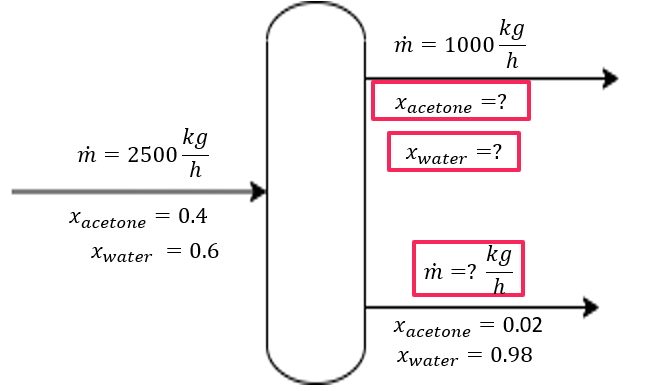
\includegraphics[width=4.54885in,height=2.71542in]{images/IntroToCHemEng2/media/image59.png}

ניתן לראות שיש 3 משתנים לא ידועים.

נספור משוואות בלתי תלויות

2 רכיבים (מים ואצטון) = שני מאזני מסה = שתי משוואות בלתי תלויות

סכום ההרכבים בזרם העליון חייב להיות שווה 1 = משוואה בלתי תלויה אחת

מפרט -- אין נתונים שלא התייחסנו אליהם

חוקים פיסיקליים -- אין חוקים המשפיעים על המערכת הזו.

סך הכל 3 משוואות בלתי תלויות

נחשב דרגות חופש

\[N_{DOF} = N_{unknowns} - N_{equations} = 3 - 3\]

מסקנה = הבעיה מוגדרת היטב, אפשר לגשת לכתיבת משוואות מלאה ופתרון.

בעת קביעת הרכב לא ידוע, אם הגדרנו כל אחד מהמשתנים בנפרד -- תהיה לנו
משוואת אילוץ אחת. לרוב נכתוב את זה בדרך חסכונית שבה נגדיר את אחד המשתנים
על בסיס משתני ההרכב האחרים, ואז יהיה לנו נעלם אחד פחות ומשוואת אילוץ אחת
פחות.

כאן לדוגמא במקום להגדיר את הרכב המים בזרם העליון כמשתנה נפרד היינו
יכולים להגדיר אותו מראש (כבר בתרשים) כ-\(x_{water} = 1 - x_{acetone}\).
במקרה זה היינו אומרים שיש לנו רק שני נעלמים (הרכב האצטון בזרם העליון
ומסת ספיקת השפכים) ושתי משוואות בלתי תלויות (מאזני מסה הנובעים משני
רכיבים המרכיבים את המערכת)

\subsection{סיכום שלבים בניתוח
מערכות}\label{ux5e1ux5d9ux5dbux5d5ux5dd-ux5e9ux5dcux5d1ux5d9ux5dd-ux5d1ux5e0ux5d9ux5eaux5d5ux5d7-ux5deux5e2ux5e8ux5dbux5d5ux5ea}

\ul{אלגוריתם כללי לפתרון}

\begin{itemize}
\item
  מגדירים את גבולות המערכת.
\item
  רושמים את כל הנתונים הידועים מהשאלה (ספיקות, ריכוזים, תנאי פעולה).
\item
  מגדירים את כל הנעלמים הדרושים לפתרון.
\item
  מבצעים ניתוח דרגות חופש: משווים בין מספר הנעלמים למספר משוואות מאזן
  עצמאיות.
\item
  כותבים את משוואת המאזן הכללי ואת מאזני הרכיבים הדרושים. מוצאים
  משוואות/נתונים נוספים לפי הצורך.
\item
  מציבים נתונים במשוואות ופותרים אלגברית את הנעלמים.
\item
  מבצעים בדיקת סבירות: יחידות עקביות, ריכוזים בין 0 ל־1, ספיקות חיוביות.
\end{itemize}

\ul{ניתוח דרגות חופש}

\begin{itemize}
\item
  מגדירים את המערכת והגבולות שלה.
\item
  מונים את כל הנעלמים העצמאיים הדרושים לפתרון.
\item
  מונים את כל המשוואות הבלתי־תלויות שניתן לכתוב (מאזני רכיבים, מאזן
  כולל, קשרי שיווי משקל, משוואות תהליך וכדומה).
\item
  מחשבים: \(N_{DOF} = n_{unkowns} - n_{indp.eq.}\)
\item
  מפרשים את התוצאה:

  \begin{itemize}
  \item
    \(N_{DOF} = 0\)המערכת מוגדרת ופתירה.
  \item
    \(N_{DOF} > 0\)חסר מידע -- יש למצוא מידע חסר או להניח הנחות
    רלוונטיות
  \item
    \(N_{DOF} < 0\)עודף מידע, יש לזהות כפילויות ולוותר על אילוצים
    מיותרים.
  \end{itemize}
\end{itemize}

\section{מאזנים על מערכות מרובות יחידות (ללא תגובה
כימית)}\label{ux5deux5d0ux5d6ux5e0ux5d9ux5dd-ux5e2ux5dc-ux5deux5e2ux5e8ux5dbux5d5ux5ea-ux5deux5e8ux5d5ux5d1ux5d5ux5ea-ux5d9ux5d7ux5d9ux5d3ux5d5ux5ea-ux5dcux5dcux5d0-ux5eaux5d2ux5d5ux5d1ux5d4-ux5dbux5d9ux5deux5d9ux5ea}

\subsection{עקרונות כללים בפתרון מערכות מרובות
יחידות}\label{ux5e2ux5e7ux5e8ux5d5ux5e0ux5d5ux5ea-ux5dbux5dcux5dcux5d9ux5dd-ux5d1ux5e4ux5eaux5e8ux5d5ux5df-ux5deux5e2ux5e8ux5dbux5d5ux5ea-ux5deux5e8ux5d5ux5d1ux5d5ux5ea-ux5d9ux5d7ux5d9ux5d3ux5d5ux5ea}

עד כה ניתחנו מערכות המכילות יחידה אחת, במקרים אלו התמונה לרוב ברורה: אין
יותר מדי אפשרויות מבחינת הגבולות שמגדירים, הזרמים שמסמנים והמאזנים
שפותרים. אבל תהליכים תעשייתיים אמיתיים מורכבים בנויים כרצף של יחידות
פעולה - ערבוב, חימום, ריאקציה, הפרדה - שכל אחת מהן משפיעה על הבאה אחריה.
ברגע שמחברים אותן למערכת אחת, הבעיה מפסיקה להיות תרגיל אלגברי נקודתי
והופכת לארגון של רשת זרמים, תלויות ומשוואות.

זה בדיוק המקום שבו אנליזה של מערכות רבות יחידות נכנסת לתמונה. המטרה היא
לפתח דרך מסודרת להתבונן בשרשרת שלמה: לזהות אילו משתנים מופיעים בכל
יחידה, אילו משוואות עומדות לרשותנו, ואיך מעבירים מידע מחלק אחד של המערכת
לחלק אחר. בשונה ממאזן פשוט על מיכל בודד, כאן האופן שבו נבחר את המערכות
ותתי המערכות שלנו, הסדר שבו נכתוב את המאזנים, וההבנה של תלות הדדית בין
יחידות - כל אלה הופכים להיות חלק מהפתרון עצמו.

לדוגמא: נתונה מערכת המפרידה תערובת של אצטון, מתנול ומים. הנתונים בציור.
מה צריכה להיות הספיקה בזרם התחתון היוצא מעמוד הזיקוק הראשון?

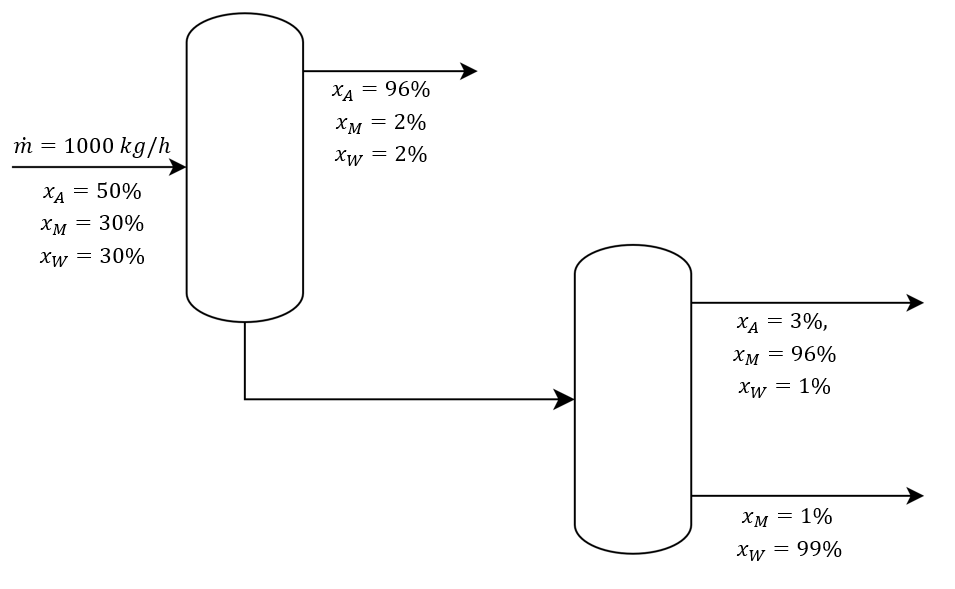
\includegraphics[width=6.39789in,height=3.94605in]{images/IntroToCHemEng2/media/image60.png}

בשלב הראשון נרצה לעשות סדר בנתונים. קודם כל נסמן כל אחד מהזרמים במספר,
ונוסיף גם את המשתנים שאינם ידועים, כך שלכל נתון יהיה סימון ייעודי.\\
בנוסף, ניתן להעביר את כל האחוזים המסתיים לשברים על מנת שיהיה יותר נוח
לעבוד איתם.\\
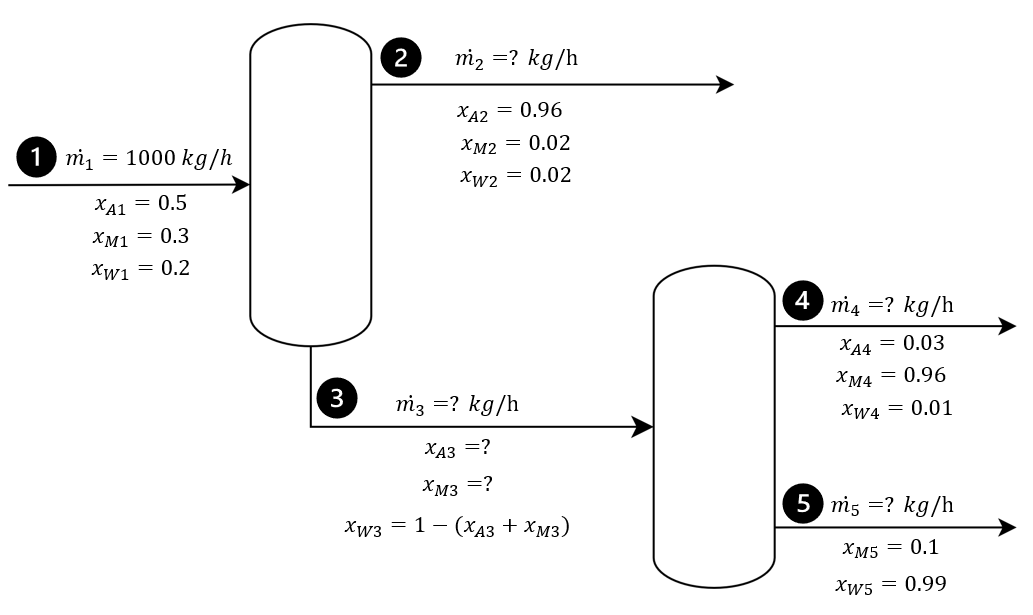
\includegraphics[width=6.5in,height=3.87014in]{images/IntroToCHemEng2/media/image61.png}

משתנים לא ידועים -
\({\dot{m}}_{2},{\dot{m}}_{3},{\dot{m}}_{4},{\dot{m}}_{5},x_{A3},\ x_{M3}\)

הנחות -- מצב עמיד, אחוז האצטון בזרם 5 זניח \(x_{A5} = 0\)

כעת נסתכל על המערכות האפשריות. ניתן להסתכל על המערכת המלאה, וניתן להסתכל
על כל אחת מעמודות הזיקוק בנפרד. עבור כל אחת מהאפשרויות נעשה ניתוח דרגות
חופש כדי לבדוק האם יש לנו מספיק נתונים ומה הסדר המועדף להתמודדות.\\
עבור כל אפשרות נצייר את גבול המערכת ונסתכל על כל החיצים שחוצים את הגבול.
חשוב לזכור שחץ שאינו נחסם על ידי מיכל או חיבור ניתן להתייחס אליו כאילו
מתקדם עד אינסוף ולכן נאריך חיצים קצרים לבדוק האם הם חוצים את גבול המערכת

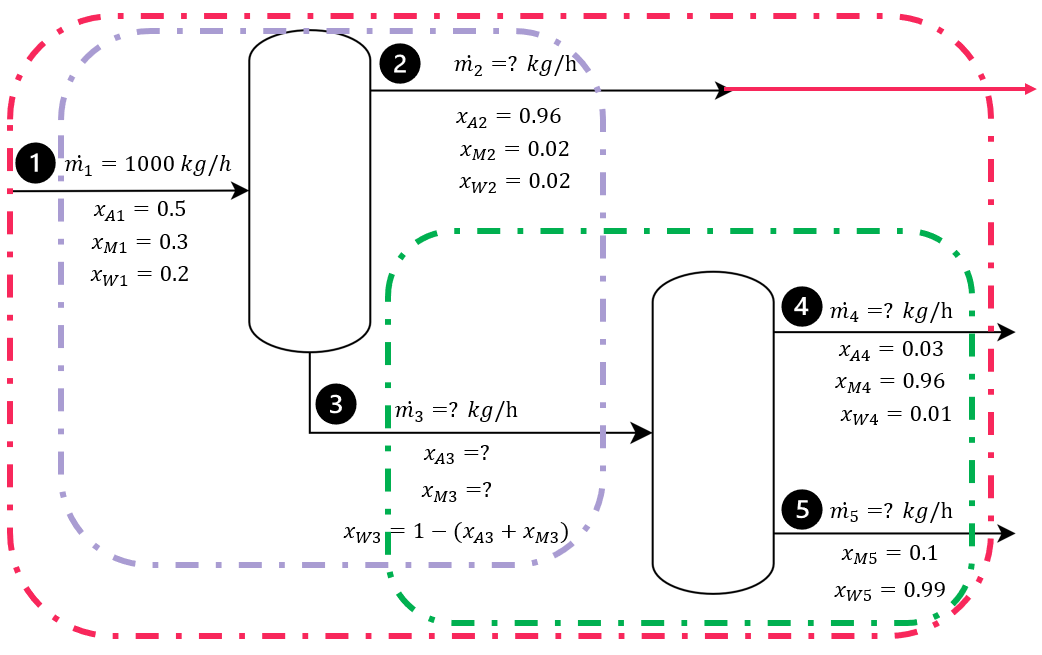
\includegraphics[width=6.5in,height=4.08611in]{images/IntroToCHemEng2/media/image62.png}

\textbf{\ul{המערכת הכוללת -}}

המשתנים שאינם ידועים הם \({\dot{m}}_{2},{\dot{m}}_{4},{\dot{m}}_{5}\)
ולכן \(n_{unknowns} = n_{U} = 3\)

יש לנו שלושה רכיבים המרכיבים את הזרמים (מים, אצטון ומתנול) ולכן נוכל
לכתוב 3 מאזני מסה

\(n_{indepenent_{equations}} = n_{E} = 3\) ז"א 3 משוואות בת"ל.

ניתוח דרגות חופש
\(\mathbf{n}_{\mathbf{U}}\mathbf{-}\mathbf{n}_{\mathbf{E}}\mathbf{= 3 - 3 = 0}\)
המערכת הכוללת \textbf{פתירה}

\textbf{\ul{עמוד הזיקוק הראשון -}}

\ul{אם ננסה לפתור את עמוד הזיקוק לפני שפתרנו את המערכת הכוללת --}

המשתנים שאינם ידועים הם \({\dot{m}}_{2},{\dot{m}}_{3},x_{A3},x_{M3}\ \)
ולכן \(n_{unknowns} = n_{U} = 4\)

יש לנו שלושה רכיבים המרכיבים את הזרמים (מים, אצטון ומתנול) ולכן נוכל
לכתוב 3 מאזני מסה

\(n_{indepenent_{equations}} = n_{E} = 3\) ז"א 3 משוואות בת"ל.

ניתוח דרגות חופש
\(\mathbf{n}_{\mathbf{U}}\mathbf{-}\mathbf{n}_{\mathbf{E}}\mathbf{= 4 - 3 = 1}\)
המערכת הכוללת \textbf{לא פתירה}

\ul{אבל אם ננסה לפתור אותו אחרי שפתרנו את המערכת הכוללת} -
\(\dot{m_{2}}\) ידוע ולכן

המשתנים שאינם ידועים הם \({\dot{m}}_{3},x_{A3},x_{M3}\ \) ולכן
\(n_{unknowns} = n_{U} = 3\)

יש לנו שלושה רכיבים המרכיבים את הזרמים (מים, אצטון ומתנול) ולכן נוכל
לכתוב 3 מאזני מסה

\(n_{indepenent_{equations}} = n_{E} = 3\) ז"א 3 משוואות בת"ל.

ניתוח דרגות חופש
\(\mathbf{n}_{\mathbf{U}}\mathbf{-}\mathbf{n}_{\mathbf{E}}\mathbf{= 3 - 3 = 0}\)
המערכת הכוללת \textbf{פתירה}

**בשלב זה למעשה נסיים למצוא את כל הנעלמים, אבל נעשה ניתוח על עמוד הזיקוק
השני לצורך המחשה**

\textbf{עמוד הזיקוק השני}

{[}אם ננסה לפתור קודם כל את עמוד הזיקוק השני --{]}\{.underline\} המשתנים
שאינם ידועים הם
\({\dot{m}}_{3},{\dot{m}}_{4},{\dot{m}}_{5},x_{A3},x_{M3}\ \) ולכן
\(n_{unknowns} = n_{U} = 5\)

יש לנו שלושה רכיבים המרכיבים את הזרמים (מים, אצטון ומתנול) ולכן נוכל
לכתוב 3 מאזני מסה

\(n_{indepenent_{equations}} = n_{E} = 3\) ז"א 3 משוואות בת"ל.

ניתוח דרגות חופש
\(\mathbf{n}_{\mathbf{U}}\mathbf{-}\mathbf{n}_{\mathbf{E}}\mathbf{= 5 - 3 = 2}\)
המערכת הכוללת \textbf{לא פתירה}

\ul{אבל אם ננסה לפתור את עמוד הזיקוק השני אחרי שפתרנו את המערכת הראשית}

\({\dot{m}}_{4},{\dot{m}}_{5}\) -- ידועים, ולכן יהיו לנו רק 3 משתנים
משתנים ו3 משוואות בת"ל והמערבת תהיה \textbf{פתירה}

\textbf{ואנחנו רואים שהדרך המועדפת היא קודם כל לפתור את המערכת הכוללת
ולאחר מכן את עמוד הזיקוק הראשון, ולאחר מכן נוכל לבצע בדיקת שפיות באמצעות
השלמת המאזנים על עמוד הזיקוק השני.}

כעת ניתן להתחיל לפתור

מערכת כוללת -
\({\dot{m}}_{1} = {\dot{m}}_{2} + {\dot{m}}_{4} + {\dot{m}}_{5}\)

מאזן על האצטון -
\({\dot{m}}_{1}x_{A1} = {\dot{m}}_{2}x_{A2} + {\dot{m}}_{4}x_{A4} + {\dot{m}}_{5}x_{A5}\)

מאזן על המתנול -
\({\dot{m}}_{1}x_{M1} = {\dot{m}}_{2}x_{M2} + {\dot{m}}_{4}x_{M4} + {\dot{m}}_{5}x_{M5}\)

הצבה

\[1000\frac{kg}{h} = {\dot{m}}_{2} + {\dot{m}}_{4} + {\dot{m}}_{5}\]

\[1000\frac{kg}{h}*0.5 = {\dot{m}}_{2}*0.96 + {\dot{m}}_{4}*0.03 + {\dot{m}}_{5}*0\]

(תזכורת -- אחוז האצטון בזרם 5 זניח)

\[1000\frac{kg}{h}*0.3 = {\dot{m}}_{2}*0.02 + {\dot{m}}_{4}*0.096 + {\dot{m}}_{5}*0.01\]

כעת יש שלוש משוואות עם שלושה נעלמים ובעזרת קצת אריתמתיקה נפתור ונקבל

\[{\dot{m}}_{2} = 511.462,\ \ {\dot{m}}_{4} = 299.879,\ \ {\dot{m}}_{5} = 188.659\]

ולכן הערכה מיטבית של המשתנים (הגדרה מקלה של שתי ספרות משמעותיות)

\[{\dot{m}}_{2} = 510\frac{kg}{h},\ \ {\dot{m}}_{4} = 300\frac{kg}{h},\ \ {\dot{m}}_{5} = 190\frac{kg}{h}\]

\{ עצירה לבדיקת שפיות לפני שממשיכים- מאחר ואנחנו מפרידים תערובת למרכיבים
שלה, אנחנו מצפים שהערכים יהיו קרובים (אך לא זהים) לחלק היחסי מהתערובת\}

כעת נעבור לעמוד הזיקוק הראשון

\[Mass\ balance:\ \ \ \ \ {\dot{m}}_{1} = {\dot{m}}_{2} + {\dot{m}}_{3}\]

\[Acetone\ balance:\ \ \ \ \ {\dot{m}}_{1}x_{A1} = {\dot{m}}_{2}x_{A2} + {\dot{m}}_{3}x_{A3}\]

\[Methanol\ balance:\ \ \ \ {\dot{m}}_{1}x_{M2} = {\dot{m}}_{2}x_{M2} + {\dot{m}}_{3}x_{M3}\]

נציב

\[1000\frac{kg}{h} = 510\frac{kg}{h} + {\dot{m}}_{3}\]

\[1000\frac{kg}{h}*0.5 = 510\frac{kg}{h}0.96 + {\dot{m}}_{3}x_{A3}\]

\[1000\frac{kg}{h}*0.3 = 510\frac{kg}{h}*0.02 + {\dot{m}}_{3}x_{M3}\]

ואחרי קצת אריתמתיקה נקבל

\[{\dot{m}}_{3}\  = \ 490\ ,\ \ \ x_{A3} = 0.021224,\ \ \ \ \ x_{M3} = 0.59143\]

ולכן הערכה מיטבית של הערכים

\[{\dot{m}}_{3}\  = \ 490\frac{kg}{h}\ ,\ \ \ x_{A3} = 0.021,\ \ \ \ \ x_{M3} = 0.59\]

\{בדיקת שפיות רגעית -- רוב האצטון יצא בזרם העליון, ולכן סביר שריכוז
האצטון בזרם התחתון יהיה נמוך\}

נבדוק על ידי הצבה של מאזן המסה הכולל של עמוד הזיקוק השני

\[{\dot{m}}_{3} = {\dot{m}}_{4} + {\dot{m}}_{5}\  = > \ \ \ \ 490\frac{kg}{h} = 300\frac{kg}{h} + 190\frac{kg}{h}\]

ומצאנו את כלל הספיקות ואת ההרכב של זרם 3.

\[{\dot{m}}_{2} = 510\frac{kg}{h},\ \ \ \ {\dot{m}}_{3}\  = \ 490\frac{kg}{h},\ \ {\dot{m}}_{4} = 300\frac{kg}{h},\ \ {\dot{m}}_{5} = 190\frac{kg}{h}\]

\[x_{A3} = 0.021,\ \ \ \ \ x_{M3} = 0.59\]

\begin{tcolorbox}[enhanced jigsaw, colback=white, arc=.35mm, coltitle=black, breakable, toptitle=1mm, leftrule=.75mm, colbacktitle=quarto-callout-tip-color!10!white, opacitybacktitle=0.6, bottomtitle=1mm, titlerule=0mm, opacityback=0, colframe=quarto-callout-tip-color-frame, title=\textcolor{quarto-callout-tip-color}{\faLightbulb}\hspace{0.5em}{עצה}, rightrule=.15mm, bottomrule=.15mm, toprule=.15mm, left=2mm]

לחשוב כמו מהנדס.ת: למה אכפת לנו מזרם הביניים?

לכאורה, אם חישבנו את הספיקות הסופיות -
\({\dot{m}}_{2},{\dot{m}}_{4},{\dot{m}}_{5}\) אנחנו יכולים להעריך כמה
קיבלנו מכל תוצר. מדוע חשוב לנו לדעת מה קורה בזרם שמחבר בין היחידות? יש
סיבות רבות, נפרט כאן מספר דוגמאות פשוטות:

\begin{itemize}
\item
  תכנון ציוד (Sizing): נניח שאנחנו צריכים לקנות את המשאבה שמעבירה את
  הנוזל מיחידה 1 ליחידה 2, או לתכנן את הקוטר של עמוד הזיקוק השני. אם לא
  נדע כמה חומר עובר שם ליחידת זמן (הספיקה \({\dot{m}}_{3}\) ) לא נוכל
  לבחור ציוד בגודל המתאים. משאבה קטנה מדי לא תעמוד בעומס, משאבה גדולה
  מדי תבזבז כסף ואנרגיה.
\item
  צריכת אנרגיה: כמות האנרגיה שצריך להשקיע ביחידה השנייהתלויה ישירות
  בכמות החומר שנכנסת אליה. צריך לדעת את הספיקה כדי לחשב את עלויות החשמל
  והקיטור של המפעל.
\item
  איתור תקלות (Troubleshooting): נניח שהתוצר הסופי בזרם 4 לא עומד
  בדרישות התהליך (לדוגמא -- מכיל יותר מדי מים) איך נמצא את מקור הבעיה?
  אולי יחידה 2 לא עובדת טוב, או שאולי יחידה 1 שלחה לה זרם "מלוכלך" מדי
  שהיא לא אמורה להתמודד איתו. מדידה וחישוב של זרם הביניים הם שלבים
  הכרחיים לצורך זיהוי הבעיה ופתרונה.
\end{itemize}

\end{tcolorbox}

\subsection{מפצל, מעקף
ותחזיר}\label{ux5deux5e4ux5e6ux5dc-ux5deux5e2ux5e7ux5e3-ux5d5ux5eaux5d7ux5d6ux5d9ux5e8}

עד כה עסקנו בתהליכים שבהם הזרימה הייתה חד-סטרית: חומרי הגלם נכנסים
ליחידה, עוברים עיבוד, והמוצרים ממשיכים הלאה. מבנה כזה נראה פשוט, אך ברוב
התהליכים הכימיים הוא אינו יעיל: חומרי גלם שלא הגיבו, תוצרים בריכוז לא
מתאים או זרם שיצא חם מדי מחייבים חשיבה מחודשת על מסלול הזרימה. במקום
תהליך ליניארי, התעשייה עושה שימוש במבנה מרושת של זרמים שמתחברים, מתפצלים
וחוזרים אחורה, כדי לשפר יעילות, לחסוך אנרגיה ולשלוט באיכות התוצרים.

כדי לבנות רשת כזו נשתמש בחמישה רכיבי זרימה בסיסיים שנפגוש בפרק זה

\textbf{צומת ערבוב (Mixer)} - נקודת מפגש שבה כמה זרמים מתאחדים לזרם יחיד
בעל הרכב חדש.\\
\textbf{מפצל (Splitter)} - נקודה שבה זרם אחד מתחלק למספר זרמים קטנים
יותר, תוך שמירה על אותו הרכב.\\
\textbf{מפריד (Seperator) --} נקודה שבה זרם אחד מתחלק למספר זרמים בעלי
הרכבים שונים.\\
\textbf{מעקף (Bypass)} - זרם העוקף יחידה מסוימת וחוזר להתחבר downstream
כדי לכוונן את תנאי התהליך.\\
\textbf{תחזיר (Recycle)} - החזרת חלק מזרם היציאה לנקודת ערבוב בכניסה,
לשם ניצול חוזר של חומרי גלם או שיפור יציבות התהליך.

כל אחד מהרכיבים האלה ישפיע באופן שונה על המערכת, על דרגות החופש שלה ועל
הדרך לפתרון.

\subsubsection{צומת
ערבוב}\label{ux5e6ux5d5ux5deux5ea-ux5e2ux5e8ux5d1ux5d5ux5d1}

צומת ערבוב היא נקודה בתהליך שבה שני זרמים או יותר מתאחדים לזרם יציאה
אחד. מבחינה הנדסית, זהו לרוב חיבור צנרת פשוט (חיבור T) או מכל בחישה
ייעודי. המאפיין המרכזי של צומת הערבוב הוא שתכונות זרם היציאה הן ממוצע
משוקלל של זרמי הכניסה.

\begin{enumerate}
\def\labelenumi{\arabic{enumi}.}
\item
  \textbf{מאזן מסה כולל:} סכום המסות הנכנסות שווה למסה היוצאת
  \(\left( \mathbf{\ }{\sum_{}^{}\dot{\mathbf{m}}}_{\mathbf{in}}\mathbf{=}{\dot{\mathbf{m}}}_{\mathbf{out}} \right).\)
\item
  \textbf{מאזן רכיבים:} הרכב הזרם היוצא
  \(\left( \mathbf{x}_{\mathbf{i,out}} \right)\) נקבע על פי היחס בין
  הספיקות של הזרמים המתערבבים.
\end{enumerate}

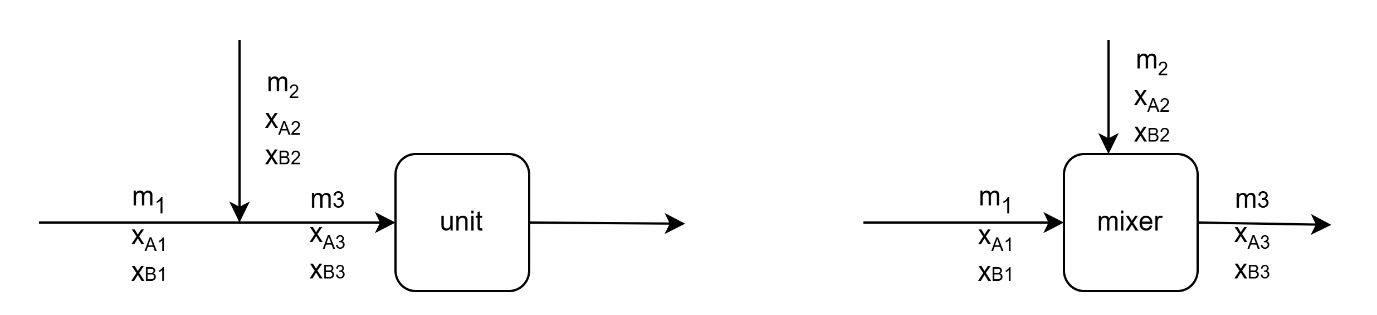
\includegraphics[width=6.20126in,height=1.41667in]{images/IntroToCHemEng2/media/image63.png}

\subsubsection{מפצל}\label{ux5deux5e4ux5e6ux5dc}

המפצל מחלק זרם אחד למספר זרמים קטנים יותר, תוך שמירה על אותו הרכב.
מבחינה חישובית זהו רכיב "פתוח": הוא יוצר נעלמים חדשים (קצבי הזרימה
ביציאות) אך מספק רק משוואת מאזן מסה אחת. לכן מפצל תמיד מוסיף דרגות חופש:
אם יש בו \(N\)יציאות, הרי שיש \(N - 1\) דרגות חופש שדורשות נתון תפעולי
כלשהו (כמו יחס זרימה או אחוז חלוקה).

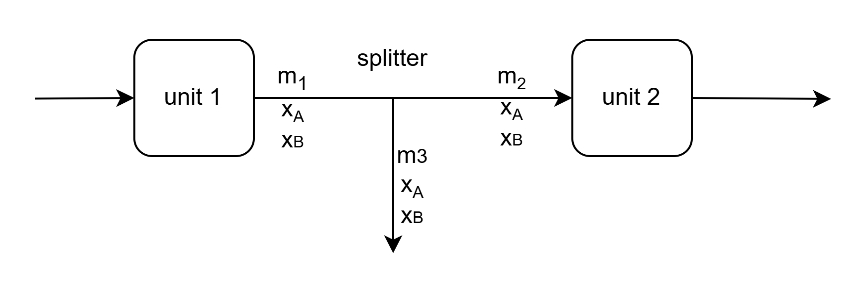
\includegraphics[width=3.9375in,height=1.3125in]{images/IntroToCHemEng2/media/image64.png}

\subsubsection{מפריד}\label{ux5deux5e4ux5e8ux5d9ux5d3}

מפריד הוא יחידת תהליך המקבלת זרם אחד ומפיקה ממנו שני זרמים או יותר, אך
בניגוד למפצל \textbf{הרכבים של הזרמים היוצאים אינם זהים להרכב הכניסה}.
ההפרדה מתבצעת באמצעות מנגנון פיזיקלי (לדוגמה: התעבות, אידוי, שקיעה,
סינון, הפרדה בין שלבים).

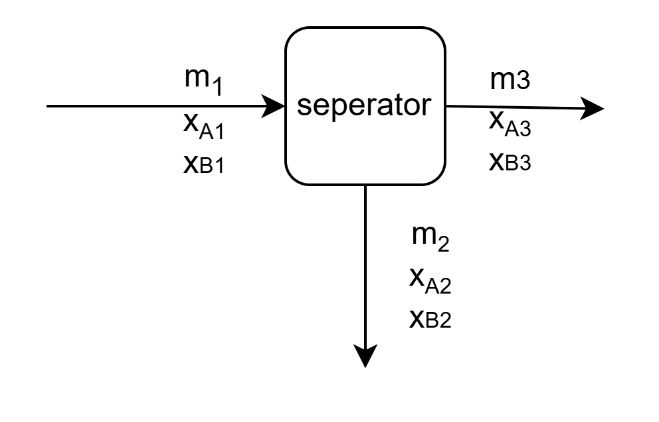
\includegraphics[width=2.99298in,height=1.70833in]{images/IntroToCHemEng2/media/image65.png}

\subsubsection{מעקף (Bypass)}\label{ux5deux5e2ux5e7ux5e3-bypass}

מעקף הוא מצב שבו חלק מן הזרימה עוקף יחידה מסוימת ומתחבר בחזרה בהמשך
התהליך (downstream). הוא מייצר דרגת חופש אחת, משום שכעת צריך להחליט כמה
מהזרם עוקף את היחידה וכמה נכנס אליה. הבחירה הזו מאפשרת לשלוט בתכונות
הסופיות (למשל טמפרטורה סופית או ריכוז).

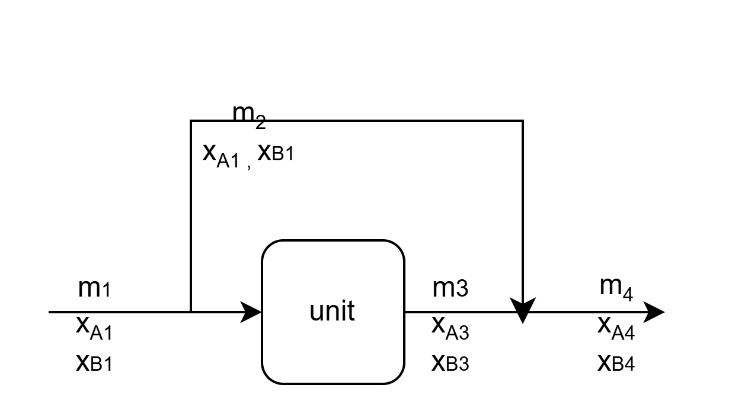
\includegraphics[width=3.3325in,height=1.47639in]{images/IntroToCHemEng2/media/image66.png}

\subsubsection{תחזיר (Recycle)}\label{ux5eaux5d7ux5d6ux5d9ux5e8-recycle}

עד כה תיארנו זרימה שמתקדמת רק קדימה. אולם בתעשייה הכימית, לעיתים נדירות
התגובה הכימית מסתיימת ב-100\% המרה במעבר אחד. מגבלות של שיווי משקל כימי
(Equilibrium) או קינטיקה איטית גורמות לכך שזרם היציאה מהריאקטור יכיל
כמות משמעותית של חומר גלם יקר שלא הגיב. זריקת חומר זה לפח (או לסביבה)
היא בזבוז כלכלי ומפגע סביבתי. הפתרון ההנדסי הוא התחזיר השבת חלק מזרם
היציאה חזרה אל הכניסה.

ברגע שקיימת לולאת תחזיר, הכניסה לריאקטור מורכבת משני מקורות. עלינו
להבדיל בין:

\begin{itemize}
\item
  \textbf{הזנה טרייה (Fresh Feed)}: חומר הגלם החדש שנכנס למערכת ממקור
  חיצוני (למשל, ממיכל האחסון).
\item
  \textbf{הזנה כוללת (Gross Feed)}: הזרם שנכנס בפועל לתוך יחידת העיבוד
  (למשל, לריאקטור). זרם זה הוא תוצאה של חיבור (בצומת הערבוב) בין ההזנה
  הטרייה לבין זרם התחזיר.\\
  \[{\dot{m}}_{Gross} = {\dot{m}}_{Fresh} + {\dot{m}}_{Recycle}\]
\end{itemize}

\pandocbounded{
\includegraphics[keepaspectratio]{images/IntroToCHemEng2/media/image70.png}}

כאשר בונים או מנתחים תרשים זרימה, כל אחד מרכיבי התהליך -- מפצל, ערבוב,
מפריד, מעקף או תחזיר -- יכול לשמש כתת־מערכת עצמאית או כחלק מתת־מערכת
גדולה יותר. הבחירה אינה טכנית אלא אסטרטגית: מטרתה לפשט את החישוב ולהגדיר
קבוצה של משתנים שניתן לסגור עליה מאזן מסה. לעיתים נוח להתחיל מיחידה
בודדת, כמו מפריד או ריאקטור, ולפתור אותה בפני עצמה; במקרים אחרים נכון
יותר להתייחס לכמה יחידות כאל מערכת אחת, משום שהקשרים ביניהן (כמו זרם
מחזור או מעקף) מכתיבים התנהגות משותפת שאי אפשר לנתח בנפרד. לכן, החלק
החשוב הוא לא רק לזהות את הרכיבים, אלא להבין מהי ``המערכת הנכונה'' עבור
שלב מסוים בפתרון -- מערכת שהמאזנים שלה עצמאיים, שהמשוואות בה ברורות,
ושדרגות החופש בה סבירות.

במפעל לייצור אשלגן חנקתי \(\left( KNO_{3} \right)\) מוזרמת תמיסת מלח
(הזנה טרייה) בקצב של \(1.0*10^{3}\frac{kg}{h}\). ריכוז המלח בהזנה הטרייה
הוא20\% משקלי. התמיסה נכנסת לצומת ערבוב, שם היא פוגשת זרם תחזיר. הזרם
המאוחד נכנס למאייד (Evaporator) המאדה חלק מהמים, כך שביציאה מהמאייד
מתקבלת תמיסה מרוכזת מאוד המכילה 50\% מלח. התמיסה המרוכזת עוברת למגבש
(Crystallizer) שם הטמפרטורה יורדת ומלח מוצק שוקע. מהמגבש יוצאים שני
זרמים: זרם אחד של גבישי \(KNO_{3}\) טהורים (ללא מים), וזרם תחזיר של
תמיסה רוויה המכילה 37\% מלח המוחזרת כולה אל צומת הערבוב בכניסה.

מהם קצב ייצור הגבישים, קצב זרימת המים המתאדים וקצב זרימת התחזיר.

פתרון:\\
אנחנו מקבלים תמיסת מלח ואנחנו מרכזים אותה על מנת שהמלח ישקע ויצאו לי
גבישים יבשים, את המים והמלח שנשארו אנחנו מעבירים להתחלה, ואנחנו רוצים
לחשב את הספיקות של א. ייצור הגבישים ב. זרימת המים ג. תחזיר

שלב ראשון -- נצייר את המערכת עם כל הנתונים (נסו לבד לפני שפותחים)

\begin{tcolorbox}[enhanced jigsaw, colback=white, arc=.35mm, coltitle=black, breakable, toptitle=1mm, leftrule=.75mm, colbacktitle=quarto-callout-note-color!10!white, opacitybacktitle=0.6, bottomtitle=1mm, titlerule=0mm, opacityback=0, colframe=quarto-callout-note-color-frame, title=\textcolor{quarto-callout-note-color}{\faInfo}\hspace{0.5em}{דיאגרמת המערכת}, rightrule=.15mm, bottomrule=.15mm, toprule=.15mm, left=2mm]

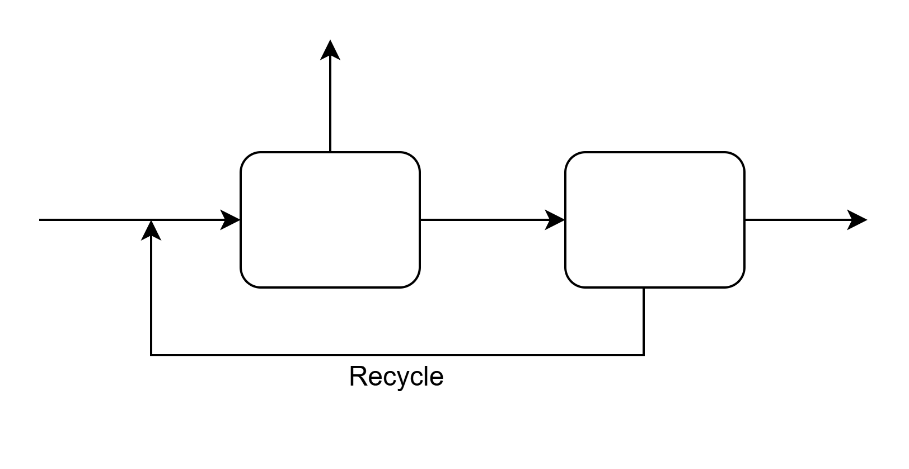
\includegraphics[width=6.5in,height=3.39653in]{images/IntroToCHemEng2/media/image67.png}

\end{tcolorbox}

הנחות: מצב עמיד, בסיס חישוב -- שעה.

מהם גבולות המערכת ותתי המערכות שאנחנו יכולים לחשב?

\begin{tcolorbox}[enhanced jigsaw, colback=white, arc=.35mm, coltitle=black, breakable, toptitle=1mm, leftrule=.75mm, colbacktitle=quarto-callout-note-color!10!white, opacitybacktitle=0.6, bottomtitle=1mm, titlerule=0mm, opacityback=0, colframe=quarto-callout-note-color-frame, title=\textcolor{quarto-callout-note-color}{\faInfo}\hspace{0.5em}{הגדרת מערכות ותתי מערכות}, rightrule=.15mm, bottomrule=.15mm, toprule=.15mm, left=2mm]

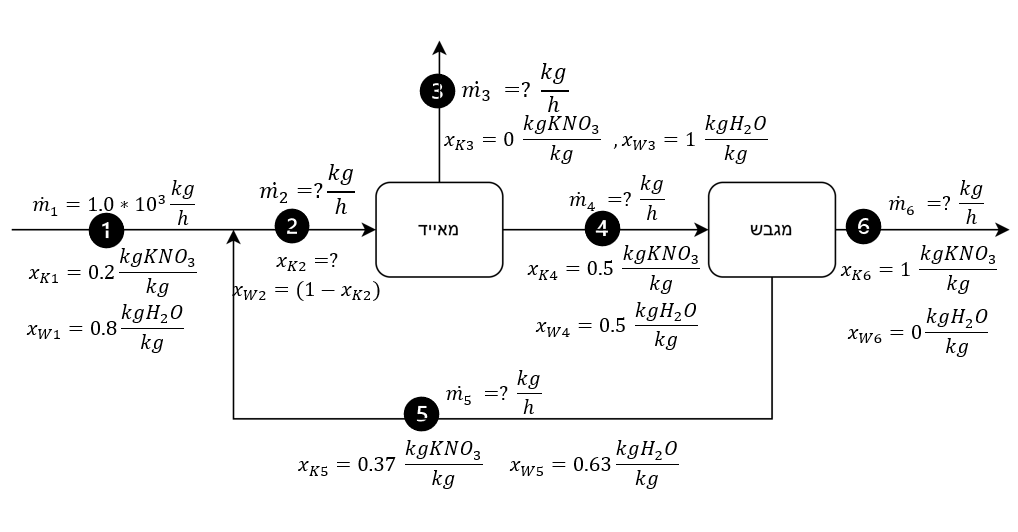
\includegraphics[width=6.5in,height=3.37847in]{images/IntroToCHemEng2/media/image68.png}

\end{tcolorbox}

נבצע ניתוח דרגות חופש לכל אחת מהמערכות.

\begin{tcolorbox}[enhanced jigsaw, colback=white, arc=.35mm, coltitle=black, breakable, toptitle=1mm, leftrule=.75mm, colbacktitle=quarto-callout-note-color!10!white, opacitybacktitle=0.6, bottomtitle=1mm, titlerule=0mm, opacityback=0, colframe=quarto-callout-note-color-frame, title=\textcolor{quarto-callout-note-color}{\faInfo}\hspace{0.5em}{ניתוח דרגות חופש}, rightrule=.15mm, bottomrule=.15mm, toprule=.15mm, left=2mm]

\begin{itemize}
\tightlist
\item
  עבור המערכת הכוללת (ורוד) הזרמים שחוצים את גבולות המערכת הם 1,3,6\\
  הנעלמים : \({\dot{m}}_{3},{\dot{m}}_{6}\) משוואות בת"ל -- שני רכיבים
  (מים, מלח) -- שתי משוואות מאזן מסה
\end{itemize}

\[DOF = 2 - 2\] \hl{המערכת פתירה}

\begin{itemize}
\tightlist
\item
  עבור נקודת הערבוב (שחור) הזרמים שחוצים את הגבולות הם 1,2,5\\
  נעלמים: \({\dot{m}}_{2},{\dot{m}}_{5},\ x_{K2}\) משוואות בת"ל- שני
  רכיבים (מים, מלח) -- שתי משוואות מאזן מסה
\end{itemize}

\[DOF = 3 - 2\]

\hl{המערכת לא פתירה}\\

\begin{itemize}
\tightlist
\item
  עבור המאייד - זרמים חוצים - 2,3,4\\
  נעלמים - \({\dot{m}}_{2},\ x_{K2},{\dot{m}}_{3},{\dot{m}}_{4}\)
  משוואות בת"ל -- שני רכיבים -- שתי משוואות מאזן מסה
\end{itemize}

\[DOF = 4 - 2\]

\hl{המערכת לא פתירה}

\begin{itemize}
\tightlist
\item
  עבור מגבש - זרמים חוצים - 4,5,6
\end{itemize}

נעלמים - \({\dot{m}}_{4},\ {\dot{m}}_{5},{\dot{m}}_{6}\) משוואות בת"ל --
שני רכיבים -- שתי משוואות מאזן מסה\\
\[DOF = 3 - 2\]

\hl{המערכת לא פתירה}\\

\end{tcolorbox}

כעת אנחנו יכולים לתכנן מסלול לפתרון.\\

\begin{tcolorbox}[enhanced jigsaw, colback=white, arc=.35mm, coltitle=black, breakable, toptitle=1mm, leftrule=.75mm, colbacktitle=quarto-callout-note-color!10!white, opacitybacktitle=0.6, bottomtitle=1mm, titlerule=0mm, opacityback=0, colframe=quarto-callout-note-color-frame, title=\textcolor{quarto-callout-note-color}{\faInfo}\hspace{0.5em}{פתרון}, rightrule=.15mm, bottomrule=.15mm, toprule=.15mm, left=2mm]

ניתן לפתור את המערכת הכללית -- ולמצוא את
\({\dot{m}}_{3},{\dot{m}}_{6}\).\\
כשיש לנו את \(,{\dot{m}}_{6}\) אנחנו יכולים להוריד דרגת חופש אחת מהמגבש,
ואז המגבש פתיר.\\
\strut \\
אחרי שאנחנו מוצאים את \({\dot{m}}_{4},\ {\dot{m}}_{5}\) גם נקודת הערבוב
תהיה פתירה, וגם המאייד יהיה פתיר. נפתור אחד מהם ונציב בשני כדי לבדוק
שהמאזן נפתר.

\end{tcolorbox}

עכשיו אפשר להתחיל לפתור.\\

\begin{tcolorbox}[enhanced jigsaw, colback=white, arc=.35mm, coltitle=black, breakable, toptitle=1mm, leftrule=.75mm, colbacktitle=quarto-callout-note-color!10!white, opacitybacktitle=0.6, bottomtitle=1mm, titlerule=0mm, opacityback=0, colframe=quarto-callout-note-color-frame, title=\textcolor{quarto-callout-note-color}{\faInfo}\hspace{0.5em}{דיאגרמת המערכת}, rightrule=.15mm, bottomrule=.15mm, toprule=.15mm, left=2mm]

\{תזכורת, בחרתי בסיס חישוב של שעה, ולכן אני יכולה לעשות את החישוב ישירות
על המסות ולא על הספיקות, התוצאה תהיה אותה תוצאה\}

\ul{המערכת הכוללת -}

מאזן מסה כולל - \(m_{1} = m_{3} + m_{6}\)

מאזן על המלח- \(m_{1}*0.2 = m_{3}*0 + m_{6}*1\)

הצבה \(1.0*10^{3}kg*0.2 = m_{6}*1\)

\[1.0*10^{3}kg*0.2 = \boxed{m_{6} = 2.0*10^{2}kg}\]

\[1.0*10^{3}kg = m_{3} + 2.0*10^{2}kg\ \  = > \ \ \ \boxed{m_{3} = 8.0*10^{2}kg}\ \]

\{בדיקת שפיות רגעית -- למלח ולמים יש רק נקודת כניסה אחת ונקודת יציאה
אחת. אם אין הצטברות, כל מה שנכנס חייב לצאת ולכן זה חייב להיות שווה לכמות
המלח שנכנסת למערכת\}

\ul{נפתור את המגבש}

מאזן מסה כולל - \(m_{4} = m_{5} + m_{6}\)

מאזן על המלח- \(m_{4}*0.5 = m_{5}*0.37 + m_{6}*1\)

הצבה -

\[m_{4} = m_{5} + 2.0*10^{2}kg\]

\[m_{4}*0.5 = m_{5}*0.37 + 2.0*10^{2}kg*1\]

\{שתי משוואות בשני נעלמים, דורש מעט אריתמתיקה\}

\[m_{4}*0.5 = (m_{4} - 2.0*10^{2}kg)*0.37 + 2.0*10^{2}kg*1\]

\[\boxed{m_{4} = 960kg}\]

\[\boxed{m_{5} = 760kg}\] \{בדיקת שפיות רגעית - במבט ראשון זה עלול
להראות מוזר, איך זה יכול להיות שהכמות בזרם m4 שווה כמעט לכל מה שנכנס אם
יש מים שמתאדים? אבל אז נזכרים שחלק מהתמיסה חוזרת חזרה וממלאת שוב את
המאייד אז זה סביר\}

נסתכל על נקודת הערבוב

מאזן מסה כולל - \(m_{1} + m_{5} = m_{2}\)

מאזן על המלח- \(m_{1}*0.2 + m_{5}*0.37 = m_{2}*x_{K2}\)

נציב

\[1000kg + 760kg = \boxed{m_{2} = 1760kg}\]

\[1000kg*0.2 + 760kg*0.37 = 1760kg*x_{K2}\]

\[x_{K2} = 0.27\]

נסתכל על המאייד לראות שהמאזן על המסה נסגר כמו שהוא אמור

מאזן מסה כולל - \(m_{2} = m_{3} + m_{4}\)

מאזן על המלח-\(m_{2}*0.27 = m_{3}*0 + m_{4}*0.5\)

נבדוק

\[1760kg = 800kg + 960kg\ \ \ \]

\[1760kg*0.27 = 800kg*0 + 960kg*0.5\]

\[1760kg*0.27 = 470kg\]

\[800kg*0 + 960kg*0.5 = 480kg\]

\end{tcolorbox}

\begin{tcolorbox}[enhanced jigsaw, colback=white, arc=.35mm, coltitle=black, breakable, toptitle=1mm, leftrule=.75mm, colbacktitle=quarto-callout-tip-color!10!white, opacitybacktitle=0.6, bottomtitle=1mm, titlerule=0mm, opacityback=0, colframe=quarto-callout-tip-color-frame, title=\textcolor{quarto-callout-tip-color}{\faLightbulb}\hspace{0.5em}{עצה}, rightrule=.15mm, bottomrule=.15mm, toprule=.15mm, left=2mm]

זהו שוויון אמפירי - כאשר כוללים את שגיאות המדידה בערכים הראשוניים, זה
הגיוני שאם מחשבים בדרכים קצת שונות מקבלים מספרים קצת שונים, כל עוד אנחנו
סביב אותו המספר והוא מסתדר מבחינת כל המערכת - אנחנו בסדר.

\end{tcolorbox}

נחזור לבדוק מה שאלו אותנו - שאלו אותנו לגבי הספיקות של הקריסטלים הנוצרים
\({\dot{m}}_{6}\), המים שהתאדו \({\dot{m}}_{3}\), וספיקת התחזיר
\({\dot{m}}_{5}\).\\
תזכורת - למען הנוחות עשינו את כל החישובים לפי בסיס חישוב של שעה, ולכן
עכשיו עלינו לחזור לספיקות.

\[Crystal\ flow\ rate\ \ \ \ \ \ \ \ \ \ {\dot{m}}_{6} = 2.0*10^{2}\frac{kgKNO_{3}}{h}\]

\[Water\ flow\ rate\ \ \ \ \ \ \ \ {\dot{m}}_{3} = 8.0*10^{2}\frac{kgH_{2}O}{h}\]

\[Recycle\ flow\ rate\ \ \ \ \ {\dot{m}}_{5} = 760\frac{kg}{h}\]

בתהליכים רב־יחידתיים גם בעיות שנראות פשוטות על הנייר הופכות במהירות
למבוכות של זרמים, הסתעפויות והפרדות. אין דרך אמיתית להתמודד עם מערכות
כאלה בלי שיטה: להגדיר את המערכת, לזהות את הזרמים, לכתוב את המאזנים
ולבדוק את דרגות החופש. הגישה השיטתית אינה כלי לימודי, אלא הכרח הנדסי -
מפני שבעולם האמיתי המאזן כמעט אף פעם לא ``נסגר'' באופן מושלם. תמיד יש
סטיות במדידות, הפסדים קטנים, ציוד שלא מתנהג בדיוק על פי המודל. המטרה
אינה למצוא פתרון מושלם מתמטית, אלא פתרון שמספיק קרוב למציאות כדי שנוכל
לקבל בעזרתו החלטות בטוחות ומושכלות

\subsection{גמלון}\label{ux5d2ux5deux5dcux5d5ux5df}

גמלון (scaling) הוא תהליך שבו מגדילים או מקטינים את גודל התהליך ההנדסי,
תוך שמירה על המבנה הכללי של התרשים ועל היחסים בין הזרמים. הרעיון הבסיסי
פשוט: תהליך שעובד היטב בקנה מידה מסוים ניתן לבצע גם בקנה מידה אחר, כל
עוד נשמרים אותם יחסי זרימה והרכבים. כך ניתן, למשל, לקחת תהליך מעבדתי קטן
ולהפיק ממנו זרימות תעשייתיות, או להפך, לצמצם תהליך גדול לצורך בדיקות
ופיתוח.

פקטור גמלון (scaling factor) הוא כלי מתמטי שמאפשר ליישם את הגמלון עצמו.
פקטור הגמלון הוא מספר שבו מכפילים את כל זרמי החומר או קצבי הזרימה
בתהליך, מבלי לשנות את ההרכב שלהם. כאשר כל הזרמים מוכפלים באותו פקטור,
התהליך נשאר מאוזן - מאזן המסה נשמר, וחלקי המסה של כל רכיב בכל זרם נותרים
זהים. כך אפשר, לדוגמה, להגדיל את התהליך פי 10, פי 300 או פי 1,000, כל
עוד ההכפלה אחידה התהליך נשאר עקבי ונכון מבחינת החישובים.

\pandocbounded{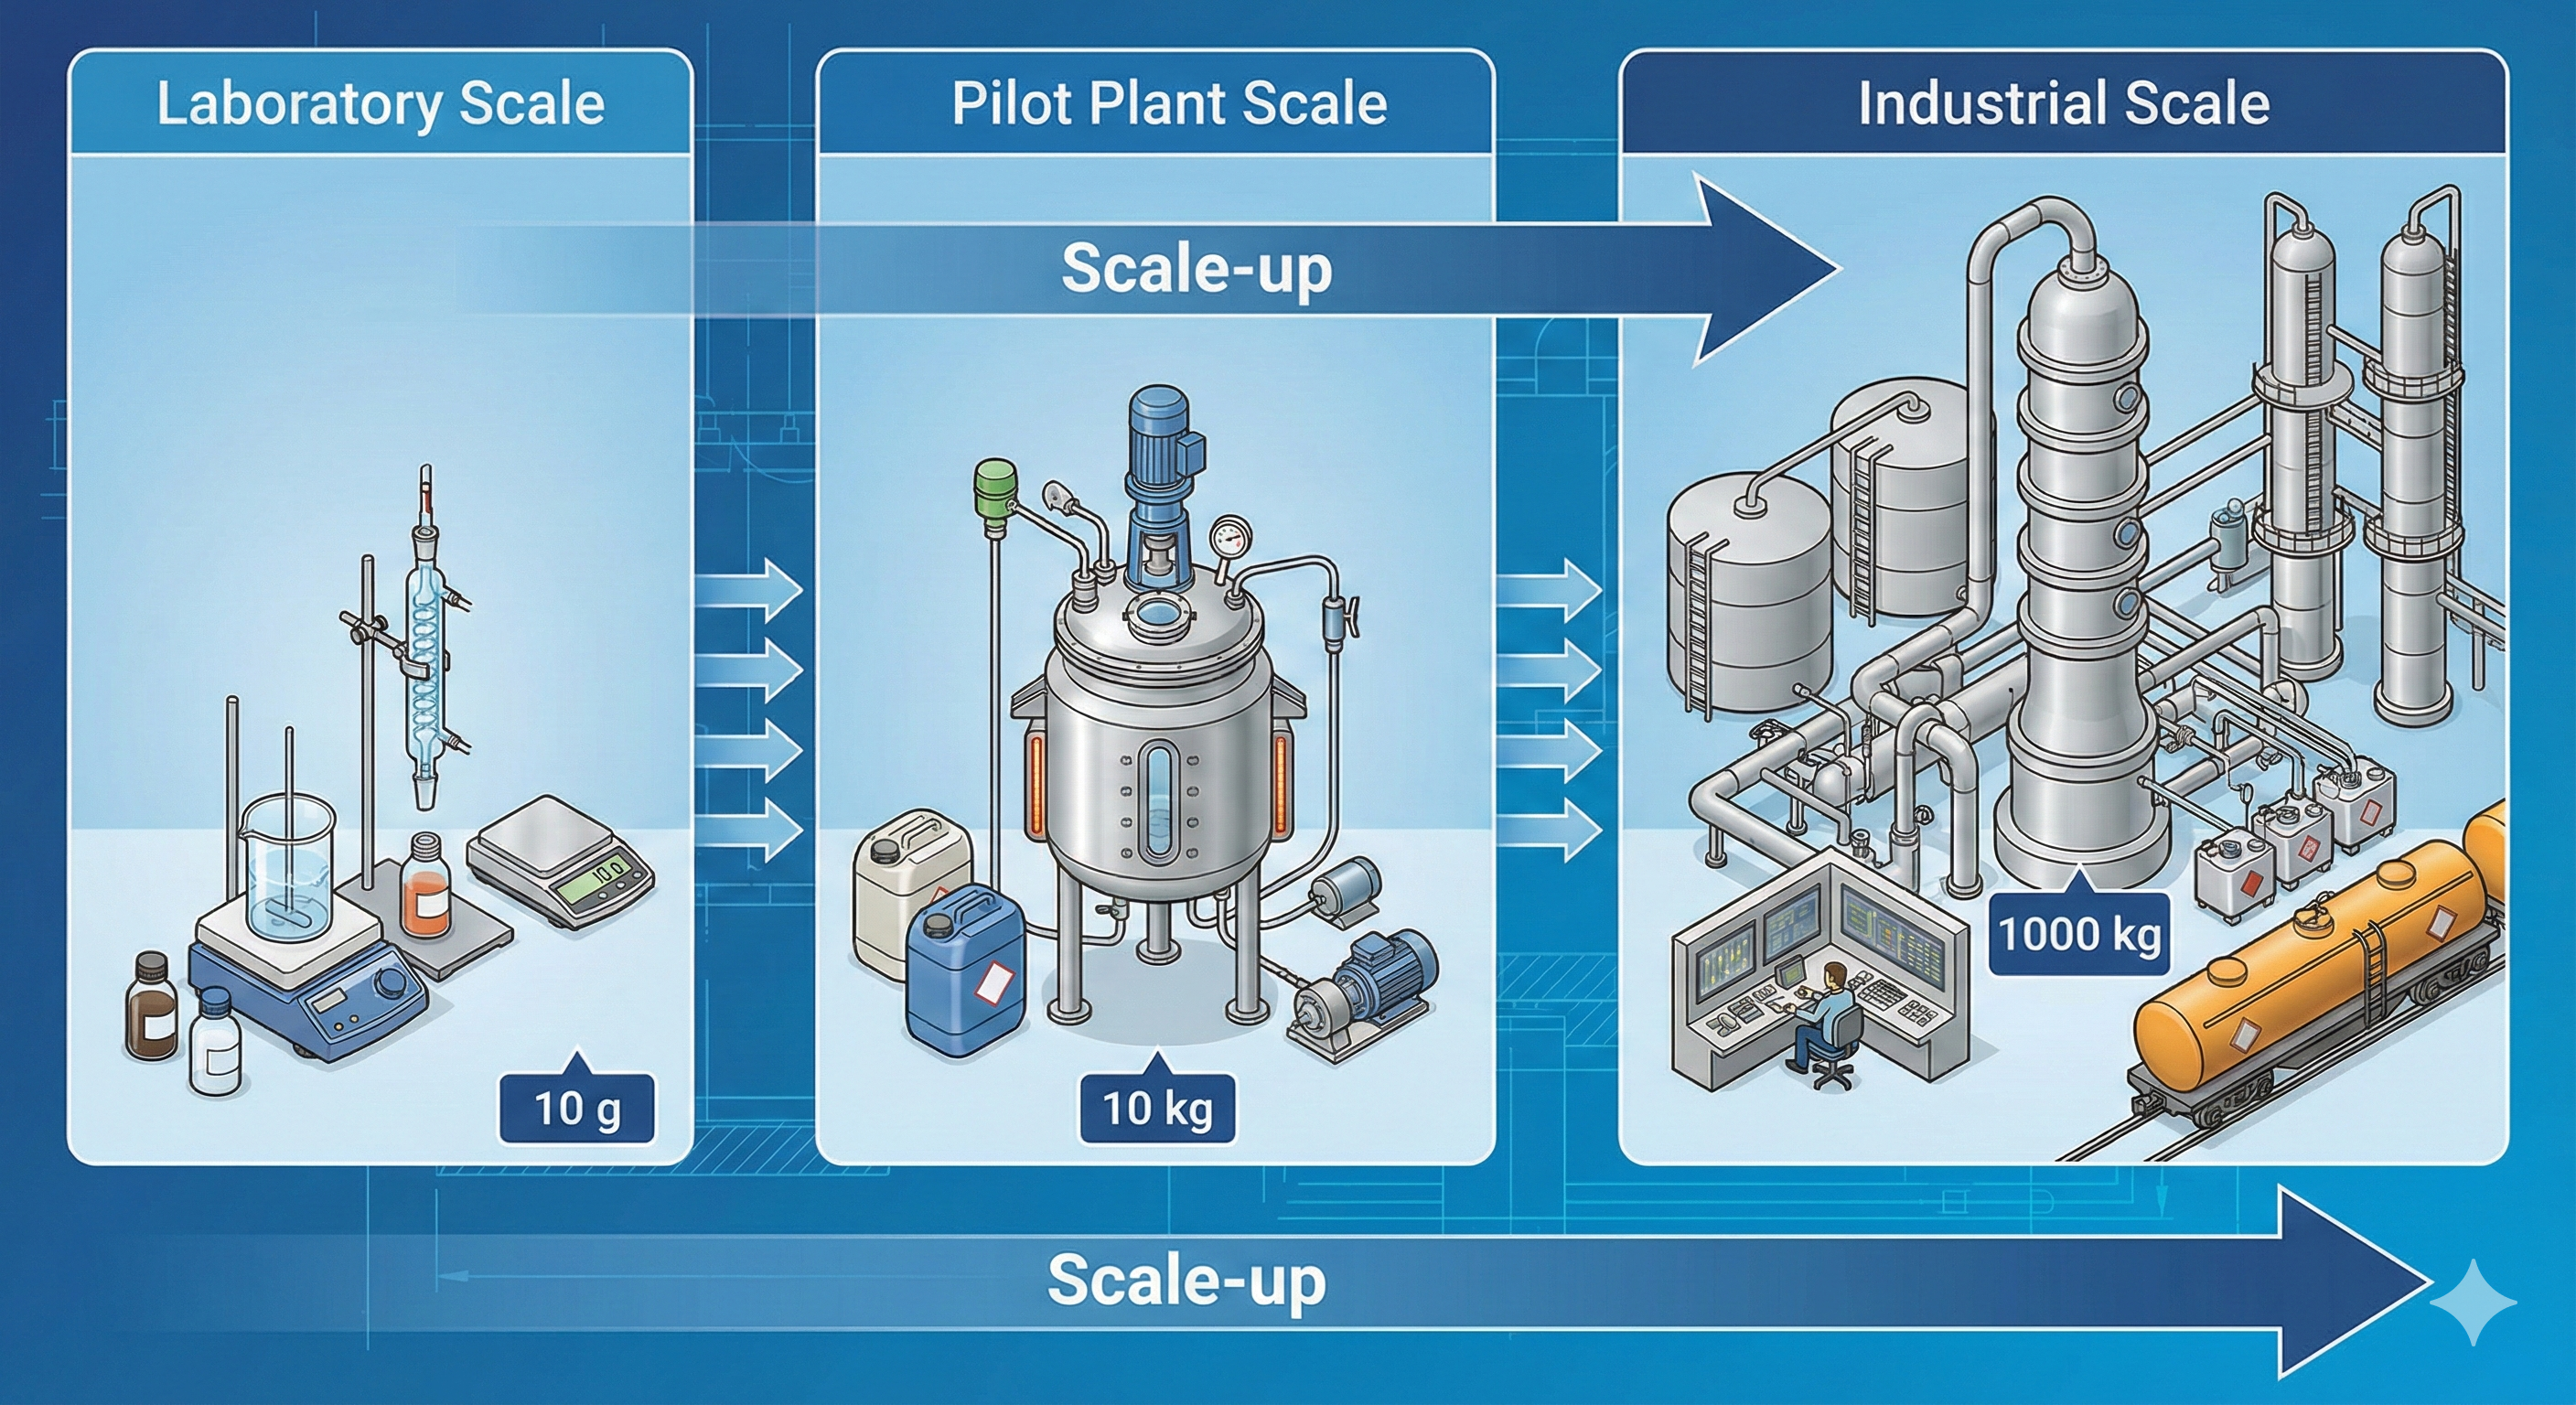
\includegraphics[keepaspectratio]{images/IntroToCHemEng2/media/image71.png}}

אולם בפועל גמלון אינו פעולה טריוויאלית. מערכות הנדסיות לא תמיד גדלות
בצורה "לינארית": תופעות פיזיקליות לפעמים משתנות באופן מהותי כאשר משנים
את קנה המידה. יחס שטח לנפח קטן ככל שמגדילים כלים, ולכן תהליכי ערבול
והעברת חום שעבדו היטב במעבדה אינם מתנהגים באותה צורה במיכל גדול. זרימה
שהייתה למינרית יכולה להפוך לטורבולנטית, מהירות ערבוב עשויה לפגוע בחומר
ביולוגי רגיש, ותהליכי הפרדה עשויים לשנות את יעילותם. לכן גמלון מצריך לא
רק הכפלה של כמויות, אלא גם בחינה של אילו שלבים בתהליך אכן גדלים באופן
ישיר, ואילו דורשים התאמות הנדסיות.

במילים אחרות, גמלון הוא שינוי בקנה המידה של התהליך, ופקטור גמלון הוא
המספר שמבצע את השינוי הזה בפועל. השימוש בפקטור גמלון הוא החלק הפשוט;
ההבנה אילו חלקים בתהליך מגיבים היטב לגמלון ואילו דורשים התאמות - זהו
האתגר ההנדסי האמיתי.

נשתמש בתהליך שפתרנו בסעיף 4.5.2 (הפרדה בין שלושה חומרים בשתי עמודות
זיקוק) וננסה לגמלן אותו

במצב הבסיס קיבלנו:

\[{\dot{m}}_{2} = 510\text{ kg/h},{\dot{m}}_{3} = 490\text{ kg/h},{\dot{m}}_{4} = 300\text{ kg/h},{\dot{m}}_{5} = 190\text{ kg/h}\]

ובהרכב הזרם 3:

\[x_{A,3} = 0.021,x_{M,3} = 0.59,x_{W,3} = 0.389\]

נניח שהמפעל רוצה להגדיל את קצב הייצור פי 10, אבל לשמור על אותה איכות
מוצרים. פקטור הגמלון הוא אם כך 10, ופשוט מכפילים בו את כל הזרמים:

\[{{\dot{m}}_{2}' = 10 \cdot 510 = 5100\text{ kg/h}
}{{\dot{m}}_{3}' = 10 \cdot 490 = 4900\text{ kg/h}
}{{\dot{m}}_{4}' = 10 \cdot 300 = 3000\text{ kg/h}
}{{\dot{m}}_{5}' = 10 \cdot 190 = 1900\text{ kg/h}
}\]

בתיאוריה, מאחר והכפלנו את הכל באותו הגורם התהליך אמור להתקיים באותו
האופן ובאותם היחסים, כך שההרכבים יהיו אותם הרכבים. למשל ההרכב של כל זרם
נשאר זהה, למשל בזרם 3:

\[x_{A,3}' = 0.021,\ \ \ \ x_{M,3}' = 0.59,\ \ \ x_{W,3}' = 0.389\]

מאזן המסה עדיין מתקיים, וכל המשוואות שכתבנו עבור המצב המקורי נשארות
נכונות גם אחרי הגמלון - פשוט עם ערכים גדולים פי 10.

איפה עלול להיווצר קושי? על הנייר, כל מה שעשינו הוא הכפלה במספר 10.
במציאות, שני הכלים בתרשים צריכים כעת להתמודד עם זרימות גדולות פי 10:
המהירויות בצנרת עולות, נפחי הכלים גדלים, זמני השהייה משתנים ותנאי ההפרדה
בעמודות עלולים להשתנות. ייתכן שעבור קצבי זרימה כאלה העמודה הראשונה ,תהיה
מוצפת או שהערבוב במיכלים כבר לא יהיה אחיד, ולכן ההרכבים בפועל בזרמים 3
ו־5 לא יהיו בדיוק אותם \(x_{A},x_{M},x_{W}\)שהנחנו בחישוב.

\subsection{סיכום}\label{ux5e1ux5d9ux5dbux5d5ux5dd-8}

\begin{itemize}
\tightlist
\item
  \textbf{חשיבה מערכתית: בחירת גבולות וניתוח תתי־מערכות}
\end{itemize}

\begin{itemize}
\item
  במערכות מרובות יחידות אין "יחידה אחת שעושים עליה מאזן", אלא רשת של
  זרמים.
\item
  בחירת גבולות המערכת היא חלק מהפתרון: מערכת גדולה מדי או קטנה מדי עלולה
  להיות לא פתירה.
\item
  לעיתים פותרים קודם את \textbf{המערכת הכוללת}, ואז יחידות פנימיות;
  לעיתים להפך.
\item
  כל מאזן נכתב רק על מה שחוצה את גבול המערכת - לכן בחירה נכונה של גבול
  היא קריטית.
\end{itemize}

\begin{itemize}
\tightlist
\item
  \textbf{דרגות חופש (DOF) ככלי עבודה מרכזי}
\end{itemize}

\begin{itemize}
\item
  מספר הנעלמים פחות מספר המשוואות הבלתי־תלויות קובע האם מערכת פתירה.
\item
  במערכות מורכבות DOF מכתיב את סדר הפתרון ולא רק את הפתרון עצמו.
\item
  \(DOF = 0\) -- מערכת פתירה. \(DOF > 0\) -- צריך נתון נוסף, \(DOF < 0\)
  -- עודף מידע/חוסר עקביות
\end{itemize}

\begin{itemize}
\item
  \textbf{חיבורים עיקריים במערכת:}

  \begin{itemize}
  \item
    מפצל, ערבוב, מפריד, מעקף ותחזיר: אלו מנגנונים שמוספים או מסירים
    אילוצים.
  \item
    מפצל ונתוני חלוקה פותחים דרגות חופש, ערבוב ומפריד מוסיפים משוואות
    מאזן, מעקף ותחזיר משנים את קישורי הזרימה ויוצרים לולאות שחייבים
    לפתור כמערכת.
  \end{itemize}
\item
  \textbf{פער בין מודל למציאות}

  \begin{itemize}
  \item
    גם במערכות מרובות יחידות המאזן לעולם לא נסגר ``מושלם'': מדידות,
    הפסדים ומודלים חלקיים מייצרים סטיות. המטרה היא מודל עקבי שמספיק קרוב
    למציאות כדי לתמוך בקבלת החלטות הנדסיות, לא שלמות מתמטית
  \item
    גמלון (Scaling) \textbf{-} כפל כל הזרמים באותו פקטור משאיר את
    המאזנים תקפים ומאפשר לעבור מקנה מידה ניסיוני לתעשייתי, אבל במציאות
    לא כל התופעות גדלות ליניארית, ולכן צריך זהירות בפרשנות.
  \end{itemize}
\end{itemize}

\section{הכרות עם מערכות הכוללות תגובות
כימית}\label{ux5d4ux5dbux5e8ux5d5ux5ea-ux5e2ux5dd-ux5deux5e2ux5e8ux5dbux5d5ux5ea-ux5d4ux5dbux5d5ux5dcux5dcux5d5ux5ea-ux5eaux5d2ux5d5ux5d1ux5d5ux5ea-ux5dbux5d9ux5deux5d9ux5ea}

בפרקים הקודמים עסקנו בתהליכים פיזיקליים בלבד: ערבוב, חימום, דחיסה
והפרדה. במערכות אלו, זהות החומרים נשמרה - מים שנכנסו למערכת יצאו ממנה
כמים, ומתנול נשאר מתנול. משוואת המאזן הבסיסית שלנו הייתה פשוטה: מה שנכנס
חייב לצאת (במצב עמיד). כעת, אנו נכנסים ללב העשייה של הנדסת התהליכים:
\textbf{הריאקטור הכימי.} כאן, חומרי גלם הופכים למוצרים בעלי ערך, וזהות
החומרים משתנה. השינוי הזה מחייב אותנו לעדכן את משוואת המאזן. לא עוד
\(Input\  = \ Output\) אלא משוואה המביאה בחשבון את היצירה (Generation)
והצריכה (Consumption) של החומרים. בפרק זה נרענן מושגים מכימיה כללית,
נתאים אותם לשפה ההנדסית של זרימה ותהליכים ונלמד כיצד למדל מתמטית את
השינויים הללו.

\subsection{סטויכיומטריה והיקף
תגובה}\label{ux5e1ux5d8ux5d5ux5d9ux5dbux5d9ux5d5ux5deux5d8ux5e8ux5d9ux5d4-ux5d5ux5d4ux5d9ux5e7ux5e3-ux5eaux5d2ux5d5ux5d1ux5d4}

כדי להבין כיצד מתארים מתמטית שינוי כימי, נתחיל מדוגמה פשוטה של תגובה
מוכרת. נניח שהמערכת שלנו מבצעת את התגובה:

\[2H_{2} + O_{2} \rightarrow 2H_{2}O\]

כאן מתרחש משהו חדש לחלוטין ביחס למה שראינו בתהליכים פיזיקליים: הכמויות
אינן עוד חופשיות להתנהג כרצונן. שתי מולקולות של מימן חייבות להגיב עם
מולקולה אחת של חמצן, ואם יחס זה אינו מתקיים - חלק מן החומרים יישארו ללא
שימוש. היחסים המספריים הללו, שמופיעים כמקדמים לפני שמות החומרים, הם לב
הסטויכיומטריה. \textbf{סטויכיומטריה} היא התיאור הכמותי של תגובה כימית:
היא קובעת אילו חומרים משתתפים בתגובה ובאיזה יחס מולקולרי. כל מקדם בתגובה
מאוזנת מציין כמה יחידות של אותו חומר נצרכות או נוצרות בכל "מחזור" תגובתי
אחד. במילים אחרות, המקדמים נותנים לנו את "שער החליפין" בין החומרים: לכל
יחידה של מגיב א\textquotesingle{} שנעלמת, כמה יחידות של מגיב
ב\textquotesingle{} חייבות להיעלם וכמה יחידות של תוצר יופיעו במקומן.
היחסים אינם ניתנים למשא ומתן -- הם מוכתבים על ידי הכימיה של המערכת ולכן
משמשים אבן יסוד בכל חישוב של ריאקטורים.

כאשר אנו מתארים תגובה כימית, אנו כותבים אותה בצורתה הכללית:

\[aA + bB \longrightarrow cC + dD\] המספרים \(a,b,c,d\) הם
\textbf{מקדמים סטויכיומטריים}. הם קובעים את היחס המולקולרי המדויק שבו
החומרים משתתפים בתגובה.

כלומר, הם מספרים לנו כמה יחידות מכל חומר נעלמות ונוצרות בכל "מחזור"
תגובתי אחד. אם נעלמות \(a\) יחידות של \(A\), בהכרח ייעלמו במקביל \(b\)
יחידות של \(B\) ויופיעו \(c\) יחידות של \(C\) ו־\(d\) יחידות של \(D\).
היחסים הללו אינם תלויים בקצב התגובה, בטמפרטורה או בצורה של הריאקטור --
הם נובעים מהמבנה הכימי של החומרים.

כך לדוגמא בתגובה הבאה של שריפת אמוניה:

\[4{NH}_{3} + 5O_{2} \longrightarrow 4NO + 6H_{2}O\]

המשמעות היא שבכל פעם שהתגובה מתקדמת "יחידה אחת" מבחינה כימית, נעלמים 4
מולים של אמוניה ו־5 מולים של חמצן, ובמקומם נוצרים 4 מולים של NO ו־6
מולים של מים. אם במערכת נעלמו בפועל 8 מולים של \({NH}_{3}\), אנו יודעים
מיד שנעלמו יחד איתם 10 מולים של \(O_{2}\) ונוצרו 8 מולים של \(NO\) ו־12
מולים של \(H_{2}O\). אין דרך "לשבור" את היחסים הללו: הם נגזרים מהמבנה
הכימי של המגיבים והתוצרים.

כדי שנוכל להשתמש במקדמים בצורה נוחה בתוך משוואות מאזן, נהוג לסמן אותם
באות היוונית \(\nu\) (ניו), עם אינדקס של הרכיב \(\nu_{i}\), כאשר עבור
המגיבים \(\nu_{i}\) שלילי (הם נצרכים), ועבור תוצרים \(\nu_{i}\) חיובי
(הם נוצרים).

לכן, עבור תגובת שריפה האמוניה נקבל

\[\nu_{NH_{3}} = - 4,\ \ \ \nu_{O_{2}} = - 5,\ \ \ \nu_{NO} = + 4,\ \ \ \nu_{H_{2}O} = + 6\]
הכתיבה ב־\(\nu_{i}\) תאפשר לנו בהמשך לנסח בצורה קומפקטית גם מאזני חומר
וגם ביטויים להתקדמות תגובה, כולל מצבים שבהם כמה תגובות פועלות בו זמנית
באותה מערכת.

מתוך המקדמים הסטויכיומטריים אנו גוזרים כלל פשוט אך חזק לחישובים מהירים.

היחס בין השינוי בכמות המולים של שני חומרים כלשהם בתגובה, שווה תמיד ליחס
בין המקדמים הסטויכיומטריים שלהם.

עבור כל שני חומרים \(i\) ו-\(j\) המשתתפים באותה תגובה:

\[\frac{\Delta n_{i}}{\Delta n_{j}} = \frac{\nu_{i}}{\nu_{j}}\]

אם נחזור לדוגמה של שריפת האמוניה, **
\[4{NH}_{3} + 5O_{2} \longrightarrow 4NO + 6H_{2}O\]

היחס בין החמצן לאמוניה הוא:

\[\frac{\nu_{O_{2}}}{\nu_{NH_{3}}} = \frac{- 5}{- 4} = 1.25\]

המשמעות הפיזיקלית היא קבועה: על כל 1 מול אמוניה שנצרך, חייבים להיצרך
1.25 מולים של חמצן.

כלל זה מאפשר לנו "לדלג" בין חומרים: אם ידוע לנו השינוי בחומר אחד, אנו
יכולים לחשב מיד את השינוי בכל חומר אחר מבלי לפתור את כל מערכת המשוואות.

כעת עלינו לעצור ולעדכן את תפיסת העולם שלנו לגבי מאזני מסה. עד כה,
במערכות ללא תגובה, התרגלנו לאמת פשוטה: \textquotesingle מה שנכנס -
יוצא\textquotesingle. אבל ברגע שמתרחשת תגובה כימית, המשפט הזה אינו נכון
יותר עבור המולקולות המשתתפות בתגובה, כמו תחמוצת החנקן או המים. החומרים
הללו משנים את זהותם; הם נצרכים ונוצרים, וכמות היציאה שלהם שונה מכמות
הכניסה. אז מה בכל זאת נשמר? \textbf{האטומים}. ריאקטור כימי (שאינו
גרעיני) אינו יכול ליצור או להשמיד אטומי חנקן, מימן או חמצן. הוא רק מסדר
אותם מחדש במבנים מולקולריים שונים. הסטויכיומטריה היא הביטוי המתמטי לכך
שבטבע אטומים נשמרים. כשאנו מאזנים משוואה כימית, אנו למעשה מוודאים שסך כל
האטומים מכל סוג שנכנסו לתהליך כחלק מהמגיבים, יימצאו בסופו כחלק מהתוצרים.

חשוב לזכור: העובדה שאנחנו יכולים לכתוב משוואה כימית מאוזנת על הנייר, לא
אומרת שהתגובה הזו אכן תתרחש במציאות. למשל, אנו יכולים לכתוב משוואה
מאוזנת להפכית גרפיט ליהלום:

\[C_{(graphite)} \rightarrow C_{(diamond)}\]

אטום פחמן נכנס, אטום פחמן יוצא. מבחינת מאזן אטומים -- המשוואה מושלמת.
אבל אם נכניס עיפרון לתנור, הוא לא ייצא יהלום.

כמהנדסי תהליך, אנחנו לא "ממציאים" תגובות. אנחנו משתמשים במשוואות
סטויכיומטריות רק כדי לתאר תגובות ש\textbf{ידוע לנו} (מתוך ידע בכימיה,
תרמודינמיקה או נתוני מעבדה) שהן אכן מתרחשות בתנאי התהליך שלנו. המאזן
הסטויכיומטרי הוא תנאי \textbf{הכרחי} (האטומים חייבים להישמר), אך הוא
אינו תנאי \textbf{מספיק} (התגובה צריכה להיות אפשרית כימית).

מתוך המאזנים האטומיים והמקדמים הסטויכיומטריים עולה שכמויות המולים של כל
החומרים המשתתפים בתגובה קשורים זה בזה בקשר הדוק. אם נדע כמה השתנה חומר
אחד, נדע מיד כמה השתנו כל האחרים.

התובנה הזו מובילה אותנו להגדרת משתנה חדש ויעיל במיוחד: \textbf{התקדמות
התגובה} (או \textquotesingle מידת התגובה\textquotesingle), המסומנת באות
\(\ \xi\)(קְסִי).

ניתן לחשוב על \(\xi\) כעל מונה הסופר \textquotesingle כמה פעמים התרחשה
המשוואה הכימית\textquotesingle{} במלואה. הקשר בין כמות החומר שנכנסה
למערכת (\(n_{i,in}\)), כמות החומר שיצאה (\(n_{i,out}\)), והתקדמות התגובה
היא:

\[n_{i,out} = n_{i,in} + \nu_{i}\ \xi\]

בעזרת התקדמות התגובה השינוי בכל החומרים המשתתפים בתגובה מוגדר באמצעות
נעלם אחד. כך למשל בתגובת האמוניה**
\[4{NH}_{3} + 5O_{2} \longrightarrow 4NO + 6H_{2}O\]

\begin{itemize}
\item
  עבור אמוניה: \(n_{NH_{3}} = n_{NH_{3,}0} - 4\xi\ \)
\item
  עבור חמצן: \(n_{O_{2}} = n_{O_{2,}0} - 5\xi\)
\item
  עבור תחמוצת החנקן: \(n_{NO} = n_{NO,0} - 4\xi\)
\item
  עבור מים: \(n_{H_{2}O} = n_{H_{2}O,0} - 6\xi\)
\end{itemize}

ללא \(\xi\), היינו צריכים להתמודד עם 4 משתני יציאה לא ידועים (כמות
האמוניה שיצאה, כמות החמצן שיצאה, וכו\textquotesingle), אבל בעזרתו אנו
יכולים לבטא את היציאה של כל ארבעת החומרים בעזרת משתנה נעלם אחד בלבד.

\subsection{המרה (Conversion, היפוך): הפער בין התיאוריה למה שקורה
בפועל.}\label{ux5d4ux5deux5e8ux5d4-conversion-ux5d4ux5d9ux5e4ux5d5ux5da-ux5d4ux5e4ux5e2ux5e8-ux5d1ux5d9ux5df-ux5d4ux5eaux5d9ux5d0ux5d5ux5e8ux5d9ux5d4-ux5dcux5deux5d4-ux5e9ux5e7ux5d5ux5e8ux5d4-ux5d1ux5e4ux5d5ux5e2ux5dc.}

כאשר אנו מתכננים ריאקטור, אחת השאלות הראשונות שמעסיקות אותנו כמהנדסים
היא: מהי כמות התוצר המקסימלית שניתן לייצר? התשובה לשאלה הזו תלויה גם
בכימיה של התגובה וגם בתנאים המערכת שנקבעים על ידינו. כיצד נעריך את
ונשפיע על כמות התוצר?

\subsubsection{מגיב מגביל (Limiting reactant) ומגיבים בעודף (Excess
reactents)}\label{ux5deux5d2ux5d9ux5d1-ux5deux5d2ux5d1ux5d9ux5dc-limiting-reactant-ux5d5ux5deux5d2ux5d9ux5d1ux5d9ux5dd-ux5d1ux5e2ux5d5ux5d3ux5e3-excess-reactents}

המשוואה הסטויכיומטרית מגדירה את יחסי הכוחות, אבל אנחנו מחליטים כמה אנחנו
מזרימים למערכת. השאלה הראשונה שנשאל את עצמינו תהיה "מי המגיב שייגמר
ראשון אם התגובה תמשיך עד הסוף?" זהו המגיב המגביל.

המגיב המגביל הוא המגיב שיגמר ראשון אם התגובה תתרחש במלואה, הוא קובע את
גבול היכולת של התגובה. גם אם כל שאר החומרים זמינים בשפע, לא ניתן לייצר
יותר תוצר מהכמות הנגזרת מכמותו של המגיב המגביל.

ברגע שיש לנו זרם הזנה מוגדר, אנו יכולים לזהות את המגיב המגביל והוא זה
שקובע את "תקרת הזכוכית" של התהליך.

מגיבים בעודף הם כל שאר החומרים שנשארים במערכת בכמות גדולה יותר מזו
הנדרשת לפי היחס הסטויכיומטרי

גם אם שאר החומרים זמינים בשפע (בעודף), לא ניתן לייצר יותר תוצר ממה
שמאפשרת כמותו של המגיב המגביל. כמות תיאורטית זו נקראת לעיתים "הייצור
המקסימלי האפשרי".

כדי להגדיר באופן כמותי את היתרה של המגיבים שאינם המגיב המגביל,\\
נשתמש ב\textbf{שבר העודף} (Fractional Excess)

\[Fractional\, Excess = \frac{n_{fed} - n_{stoich}}{n_{stoich}}\ \ \ \ \ ,\ \ \ \ n_{stoich} = n_{limiting}*\frac{\nu_{}}{\nu_{limiting}}\]

כאשר:

\(n_{fed}\) הכמות שהוזנה בפועל למערכת.

\(n_{stoich}\) הכמות התיאורטית שהיתה נדרשת אילו המגיב המגביל היה מגיב
במלואו.

באותו אופן ניתן להגדיר את אחוז העודף (Excess \%) אם נכפיל את שבר העודף
ב100\%.

\subsubsection{שיווי משקל
כימי}\label{ux5e9ux5d9ux5d5ux5d5ux5d9-ux5deux5e9ux5e7ux5dc-ux5dbux5d9ux5deux5d9}

עד כה הנחנו שריאקציה מתקדמת בכיוון אחד: מגיבים הופכים לתוצרים. אולם
בטבע, תהליכים רבים הם \textbf{הפיכים}. מערכות אלו, במקביל לתגובה הישירה
\((A\  \rightarrow B)\)מתרחשת גם התגובה ההפוכה \((B \rightarrow A)\) אנו
מסמנים תגובות אלו בחץ כפול:

\[aA\  + \ bB\  \rightleftharpoons cC\  + \ dD\]

ככל שריכוז התוצרים עולה, קצב התגובה ההפוכה גדל. בשלב מסוים, קצב היצירה
של התוצרים משתווה בדיוק לקצב הפירוק שלהם חזרה למגיבים. במצב זה, למרות
שהמולקולות ממשיכות להגיב ללא הרף, ב\textbf{רמת המאקרו אין שינוי בהרכב
המערכת}. למצב זה אנו קוראים \textbf{שיווי משקל כימי} (Chemical
Equilibrium).\\

קבוע שיווי משקל הוא היחס בין ריכוזי התוצרים לריכוזי המגיבים במצב שיווי
משקל הוא ערך קבוע עבור תגובה מסויימת בטמפרטורה מסויימת. בצורתו הפשוטה
(עבור ריכוזי החומרים), הוא מוגדר כך:

\[K(T) = \frac{\lbrack C\rbrack^{c}\lbrack D\rbrack^{d}}{\lbrack A\rbrack^{a}\lbrack B\rbrack^{b}}\]

את ערכיו של \(K\) ניתן למצוא באופן נסיוני או להשתמש בנתונים מהספרות
המקצועית. לרוב, ערכי קבוע שיווי המשקל נתונים עבור מצב סטנדרטי
\(\mathbf{2}\mathbf{5}^{\mathbf{\circ}}\mathbf{C}\), אך ניתן לתקן אותם
לטמפרטורת התהליך בפועל בעזרת משוואות תרמודינמיות (כמו משוואת ואן-הוף).

\textbf{חישוב הרכב בשיווי משקל}

כיצד נדע מה יהיה הרכב התערובת הסופי? בהנחה שקבוע שיווי המשקל וריכוזי
החומרים בכלי בתחילת התהליך מוכרים לנו, נוכל להשתמש בהם על מנת לחשב את
הרכב המערכת בשיווי משקל. נגדיר את הכמות בפועל של כל אחד מהחומרים באמצעות
מקדם התקדמות התגובה (\(\xi\)).

\[n_{i,eq} = n_{i,0} + \nu_{i}\xi\]

כאשר \(\xi\) מוגדר ביחידות של מול (בהתאם לשאר המשוואה).

ההצבה בקבוע שיווי משקל דורשת להגדיר את הרכב החומרים השונים באמצעות ריכוז
החומרים במול לליטר (\(M\)), או באמצעות הלחצים החלקיים. על מנת לעבור
לריכוזים עלינו לחלק את הביטוי בנפח הכלי (\(V\)).

\[\frac{n_{i,eq}}{V} = \frac{n_{i,0}}{V} + \nu_{i}\xi\ \ \  = > \ \ C_{i,eq} = C_{i,0} + \nu_{i}\xi\]

במקרה זה \(\xi\) יתקבל ביחידות של מולר (\emph{M}). בפרק 5 נדבר על גזים
ונוכל לחשב

את הביטויים הללו נציב בתוך משוואת קבוע שיווי המשקל ונקבל משוואה אלגברית
עם נעלם אחד, באמצעותה נוכל למצוא את מידת התגובה, ולחשב את הרכב המערכת
בשיווי משקל.

\textbf{עקרון לה-שטלייה (Le Chatelier)}

לפני שנבצע חישובים, עקרון לה-שטלייה מאפשר לנו לחזות איכותית לאן המערכת
תזוז בתגובה לשינויים ("עקה"). העקרון קובע שהמערכת תמיד תשאף "לתקן" את
ההפרעה:

\begin{enumerate}
\def\labelenumi{\arabic{enumi}.}
\tightlist
\item
  שינוי בהרכב (הוספה או הסרה של חומר ספציפי)
\end{enumerate}

במקרה זה אין שינוי בקבוע ש"מ (K), המערכת פשוט יצאה מאיזון רגעי, והיא
תגיב כדי לצמצם את השינוי שנכפה עליה:

\begin{itemize}
\item
  בהוספת מגיב/סילוק תוצר -- המערכת "מרגישה" שיש עודף במגיבים ביחס
  לתוצרים ותנסה לתקן זאת על ידי הפיכה של מגיבים לתוצרים, והתגובה תנועה
  קדימה.
\item
  בסילוק מגיב/הוספת תוצר - המערכת "מרגישה" שיש עודף בתוצרים ביחס למגיבים
  ותנסה לתקן זאת על ידי הפיכה של תוצרים למגיבים, והתגובה תנועה אחורה.

  \begin{enumerate}
  \def\labelenumi{\arabic{enumi}.}
  \tightlist
  \item
    שינוי בנפח או בלחץ בכלי (שינוי בכלל הריכוזים במערכת)
  \end{enumerate}
\end{itemize}

בניגוד להוספת חומר ספציפי, כאן אנו מבצעים פעולה שמשפיעה על הריכוז של כל
החומרים במערכת בו-זמנית. גם במקרה זה, הקבוע \(K\) נשאר ללא שינוי,
והמערכת מגיבה לשינוי ב"צפיפות" החלקיקים.

\begin{itemize}
\item
  בגזים: השינוי מתבצע על ידי דחיסה (העלאת לחץ/הקטנת נפח) או התפשטות
  (הורדת לחץ/הגדלת נפח).
\item
  בנוזלים: השינוי מתבצע על ידי שינוי כמות הממס (למשל, הוספת מים לדילול
  או אידוי מים לריכוז).
\end{itemize}

כיצד המערכת מגיבה?

שינויי הריכוז משפיעים על יחס המגיבים והתוצרים כך שהוא כבר אינו מקיים את
משוואת שיווי המשקל. במקרה זה המערכת תגיב בהתאם למצב הצפיפות החדש:

\begin{itemize}
\item
  כשהמערכת "צפופה" מדי (לחץ גבוה או תמיסה מרוכזת): כדי להקל על הלחץ, היא
  תשאף להקטין את מספר החלקיקים. לכן, התגובה תזוז לכיוון שבו יש פחות
  מולים (סכום המקדמים הסטויכיומטריים של הנמוך יותר).
\item
  כשהמערכת "מרווחת" מדי (לחץ נמוך או תמיסה מדוללת): נוצר "חלל" שהמערכת
  שואפת למלא. כדי לעשות זאת, היא תשאף להגדיל את מספר החלקיקים. לכן,
  התגובה תזוז לכיוון שבו יש יותר מולים (סכום המקדמים הסטויכיומטריים
  הגבוה יותר).
\end{itemize}

שימו לב: כשאנו מדברים על סכום המקדמים הסטויכיומטרים, אנו מדברים רק על
הרכיבים שמשפיעים על שיווי המשקל -גזים וחומרים מומסים. נוזלים ומוצרים לא
משפיעים על שיווי המשקל. אם סכום המקדמים הסטויכיומטריים של המגיבים שווה
לזה של התוצרים (למשל \(H_{2} + I_{2} \rightleftharpoons 2HI\)) לשינוי
הנפח או הלחץ לא יהיה שום אפקט על שיווי המשקל, שכן מספר החלקיקים נשאר זהה
בכל מקרה.

\begin{enumerate}
\def\labelenumi{\arabic{enumi}.}
\tightlist
\item
  השפעת הטמפרטורה (שינוי של \(K\))
\end{enumerate}

שינוי הטמפרטורה הוא המקרה היחיד בו ערך קבוע שיווי המשקל משתנה, והתגובה
תתקדם לכיוון הרצוי (קדימה או אחורה) על מנת להתאים את עצמה לקבוע החדש.
כדי לזכור בקלות לאן ייטה שיווי המשקל, נוח להשתמש במודל "חום כרכיב":

\begin{itemize}
\item
  בתגובה אקסותרמית (תגובה הפולטת חום) נוכל לדמיין את החום כ"תוצר". עליית
  טמפרטורה שקולה ל"הוספת תוצר". כדי לחזור לאיזון, המערכת תיאלץ ללכת
  אחורה (לכיוון המגיבים). ואנו רואים שערכו של הקבוע K קטן.
\item
  בתגובה אנדותרמית (תגובה הקולטת חום) נוכל לדמיין את החום כ"מגיב". עליית
  טמפרטורה שקולה ל"הוספת מגיב". כדי לחזור לאיזון המערכת תיאלץ ללכת קדימה
  ואנו רואים שערכו של הקבוע \(K\) גדל.
\end{itemize}

\subsubsection{מקדם המרה (Conversion
factor)}\label{ux5deux5e7ux5d3ux5dd-ux5d4ux5deux5e8ux5d4-conversion-factor}

גם כשידוע לנו המקסימום התיאורטי, במציאות התעשייתית התגובה כמעט לעולם לא
מגיעה לניצול של 100\% מהמגיב המגביל. הסיבות לכך מגוונות.

\begin{itemize}
\item
  \ul{מגבלות תרמודינמיות (שיווי משקל):} תגובות רבות הן הפיכות. במצב כזה,
  המערכת שואפת להגיע לנקודת שיווי-משקל כימי שבה קצב התגובה הקדימה שווה
  לקצב התגובה ההפוכה. בנקודה זו הריאקציה "נעצרת" (ברמת המאקרו) עוד לפני
  שכל המגיבים נצרכו.
\item
  \ul{מגבלות קינטיות (קצב תגובה):} לעיתים התגובה איטית מאוד, והגעה
  לניצול מלא דורשת זמן שהייה ארוך באופן לא סביר בתוך הריאקטור.
\item
  \ul{מגבלות סלקטיביות (תגובות לוואי):} במקרים רבים מתרחשות במקביל
  תגובות נוספות המתחרות על אותם מגיבים. חלק מהמגיב המגביל "מתבזבז" על
  יצירת תוצרי לוואי לא רצויים במקום להפוך לתוצר המבוקש.
\end{itemize}

המגבלות שמנינו למעלה אינן רק "בעיות מדעיות", אלא פקטורים שמשפיעים ישירות
על הרווחים. הנדסת תהליך טובה דורשת לנהל את המגבלות הללו כדי למקסם את
יעילות התהליך.

\textbf{התמודדות עם שיווי משקל:} כיצד נגרום למגיב יקר להגיב כמעט במלואו
בתגובה הפיכה? נשתמש בעקרון לה-שטלייה: נזין \textbf{עודף גדול של המגיב
הזול} (למשל, אוויר או מים). העודף "דוחף" את שיווי המשקל קדימה ומאלץ את
המגיב היקר (המגביל) להגיב באחוזים גבוהים יותר.

\textbf{התמודדות עם קינטיקה איטית:} ככל שהמגיבים נצרכים, קצב התגובה
יורד. כדי להשיג את ה"אחוזים האחרונים" של ההמרה, נדרש זמן עצום (וריאקטור
ענק ויקר). לכן, הכלל הכלכלי הוא \textbf{חוק התפוקה השולית הפוחתת} - עדיף
לעצור את התגובה כאשר קצב הייצור יורד מתחת לרף מסוים, להפריד את התוצרים,
ולהחזיר את חומרי הגלם שלא הגיבו לסיבוב נוסף (Recycle), מאשר לאפשר לתגובה
את הזמן הנדרש על מנת שתתרחש במלואה.

\textbf{התמודדות עם תגובות לוואי (תגובות מקבילות):} לעיתים התנאים
בריאקטור הם כאלו המאפשרים התרחשות של תגובות נוספות מעבר לתגובה הרצויה.
במקרים אלו עלינו להתחשב גם בהתקדמות התגובות האחרות על מנת למקסם את ההמרה
של התגובה הרצויה. היחס בין כמות התוצר הרצוי לכמות תוצר לוואי נקראת
בררנות או סלקטיביות Selectivity, ונדבר עליה יותר לעומק בהמשך.

כדי לכמת את הפער בין הפוטנציאל התיאורטי לבין המציאות בפועל, אנו מגדירים
את פקטור ההמרה או שבר ההמרה

פקטור ההמרה או שבר ההמרה Fractional Conversion משמש לכימות הפער בין
הפוטנציאל התיאורטי לבין המציאות בפועל. הוא מסומן לרוב ב\(\chi\) או ב
\(f\) וההגדרה מתייחסת כמעט תמיד למגיב המגביל (אלא אם צוין אחרת):

\[\chi_{A} = \frac{\text{moles of A reacted}}{\text{moles of A fed}}\]

או בנוסחה מתמטית, עבור מגיב \(A\)

\[\chi_{A} = \frac{n_{A,in} - n_{A,out}}{n_{A,in}}\]

כאשר

\(\chi_{A} = 0\) התגובה לא התקדמה כלל (כל מה שנכנס -- יצא).

\(\chi_{A} = 1\) המרה מלאה. המגיב נצרך כולו (המצב התיאורטי המקסימלי).

במרבית המקרים \(0 < \chi_{A} < 1\) - רק חלק מהמגיב הפך לתוצרים, ואנו
נרצה למקסם את \(\chi_{A}\) ככל האפשר.

\[n_{A,out} = n_{A,in}\left( 1 - X_{A} \right)\]

משוואה זו אומרת בפשטות: מה שיצא החוצה הוא מה שנכנס, מוכפל בחלק הנותר
\(\left( 1 - X_{A} \right)\)שלא הגיב.

\subsection{תגובות מרובות, ניצולת
וסלקטיביות}\label{ux5eaux5d2ux5d5ux5d1ux5d5ux5ea-ux5deux5e8ux5d5ux5d1ux5d5ux5ea-ux5e0ux5d9ux5e6ux5d5ux5dcux5ea-ux5d5ux5e1ux5dcux5e7ux5d8ux5d9ux5d1ux5d9ux5d5ux5ea}

ברוב התהליכים התעשייתיים, המפגש בין מגיבים בריאקטור לא מסתכם במסלול כימי
יחיד. חומרי הגלם שלנו \textquotesingle חשופים\textquotesingle{} למספר
אפשרויות תרמודינמיות במקביל, ועשויים להגיב בצורות שונות המובילות לתוצרים
מגוונים. בעוד מסלול אחד ייצר את המוצר המבוקש, מסלולים אחרים עשויים
להוביל לתוצרי לוואי חסרי ערך כלכלי או אפילו כאלה המזיקים לסביבה. משום
כך, האתגר ההנדסי אינו מסתכם רק בביצוע התגובה, אלא בניהול התחרות בין
המסלולים השונים: עלינו לתכנן את התנאים כך שהמסלול הרצוי יגבר על האחרים
בצורה המובהקת ביותר.

נהוג לסווג מערכות מרובות תגובות לשתי קטגוריות עיקריות:

\begin{itemize}
\tightlist
\item
  תגובות מקבילות (Parallel Reactions).
\end{itemize}

במצב זה, המגיב \(A\) יכול להשתתף במספר מסלולים שונים המתחרים זה בזה.
מסלול אחד מוביל לתוצר הרצוי \(B\), בעוד מסלול אחר "מבזבז" את המגיב
ליצירת תוצר לוואי \(C\).

\[A \rightarrow B\quad\left( \text{Desired} \right)\]

\[A \rightarrow C\quad\left( \text{Undesired} \right)\]

למשל תגובת חמצון של אתילן \(C_{2}H_{4}\). בתגובה הרצויה, אתילן מגיב עם
חמצן ליצירת אתילן-אוקסיד (\(C_{2}H_{4}O\) חומר גלם חשוב לתעשייה).
במקביל, האתילן עלול לעבור שריפה מלאה עם החמצן ליצירת פחמן דו-חמצני ומים.
האתגר כאן הוא למצוא את התנאים שיצרו העדפה לתגובה הראשונה.

\begin{itemize}
\tightlist
\item
  תגובות ממשיכות / טוריות (Series Reactions)
\end{itemize}

כאן התגובה מתרחשת בשלבים: המגיב \(A\) הופך לתוצר ביניים \(B\) אשר יכול
להמשיך להגיב ולהפוך לתוצר סופי \(C\).

\[A\, \rightarrow \, B\, \rightarrow \, C\]

במקרים מסויימים התוצר הרצוי לנו יהיה תוצר הביניים, ונרצה לעצור את המשך
התגובה. במקרים אחרים המטרה תהיה דווקא התוצר הסופי ואנחנו נצטרך לעזור
לתגובה לא להמשיך ולא לעצור בתוצר הביניים.

כאשר במערכת מתרחשת תגובה בודדת, אנו משתמשים במשתנה יחיד, \(\xi\), כדי
לתאר את השינוי בכמויות כל הרכיבים. אך מה קורה כשיש לנו שתי תגובות (או
יותר) המתרחשות במקביל?

במצב כזה, עלינו להגדיר \textbf{מידת התקדמות נפרדת לכל תגובה} כאשר

\(\xi_{1}\) הוא מונה המציין כמה מולים הגיבו לפי המשוואה הסטויכיומטרית של
תגובה 1.

\(\xi_{2}\) הוא מונה נפרד המציין כמה מולים הגיבו לפי המשוואה
הסטויכיומטרית של תגובה 2.

וכן הלאה...

הקשר בין שתי מידות ההתקדמות נוצר דרך החומרים המשותפים לשתי התגובות.
הכמות הסופית של כל חומר ביציאה היא תוצאה של השינוי המצטבר שנגרם על ידי
כל התגובות שבהן הוא משתתף.

המשוואה הכללית עבור רכיב \(i\) היא:

\[n_{i,out} = n_{i,in} + \sum_{j = 1}^{N_{reactions}}{\nu_{ij}\xi_{j}}\]

\subsubsection{מדדי ביצוע: ניצולת
(Yield)}\label{ux5deux5d3ux5d3ux5d9-ux5d1ux5d9ux5e6ux5d5ux5e2-ux5e0ux5d9ux5e6ux5d5ux5dcux5ea-yield}

המדד המרכזי להערכת יעילות הראקטור ה\textbf{ניצולת} (Yield). על פי ההגדרה
המקובלת (וזו שנשתמש בה בספר זה), הניצולת היא מדד המשווה את המציאות
לפוטנציאל המקסימלי.

הניצולת Yield מוגדרת כיחס בין כמות התוצר הרצוי שנוצרה בפועל, לבין הכמות
התיאורטית שהייתה נוצרת אילו התגובה הייתה מושלמת (ללא תגובות לוואי וללא
מגיבים שלא הגיבו).

הנוסחה לחישוב הניצולת היא:

\[\text{Yield} = \frac{\text{Moles of Desired Product Formed}}{\text{Theoretical Max Moles of Desired Product}}\]

כאשר על מנת לחשב את המכנה אנחנו מניחים שכל הכמות של המגיב \ul{המגביל}
שהוזנה לראקטור הגיבה במלואה והפכה רק לתוצר הרצוי, ללא תוצרי לוואי. לכן,
ערכה של הניצולת חייב להיות בטווח \(\text{0<Yield<1}\)

בספרים אחרים (ובתעשייה) לעיתים תיתקלו בהגדרה שונה לניצולת, המחשבת את
כמות התוצר שנוצר ביחס לכמות המגיב שהוזן (הן ביחס מולי והן ביחס מסתי).
בחישוב זה, טווח הערכים אינו מוגבל \(0 - 1\) ועשוי להשתנות דרמטית כתלות
ביחס הסטויכיומטרי ו/או במסות המולריות של החומרים, מה שהופך את ההגדרה
לפחות אינטואיטיבית להבנת היעילות הכימית בשלבי הלמידה הראשונים. עם זאת,
להגדרה זו יש ערך פרקטי רב: היא משמשת כ\textquotesingle מקדם
המרה\textquotesingle{} תפעולי, המאפשר למנהלי מפעלים לחשב במהירות מהי
כמות התוצר הסופית שתתקבל עבור כל יחידת חומר גלם שנרכשה והוכנסה לתהליך.

נתון תהליך לייצור החומר \(C\) מתוך החומר \(A\) בשני שלבים עוקבים
המבוצעים בשני ריאקטורים נפרדים לפי התהליך הבא
\(A \rightarrow B \rightarrow 2C\).

לראקטור הראשון הוזנו 100 מולים של A, וביציאה מהראקטור התקבלו 80 מולים של
תוצר הביניים B. כל הכמות הזו הוזנה לריאקטור השני וביציאה מהראקטור השני
התקבלו 120 מול של התוצר הסופי C.

מהי הניצולת של (א) השלב הראשון (ב) השלב השני (ג) הניצולת הכוללת בתהליך
ביחס להזנה המקורית?

א -- עבור השלב הראשון. מהו המקסימום התיאורטי של B שניתן היה לקבל מהזנה
של 100 מולים של A? מכיוון שהיחס הוא 1:1 המקסימום הוא 100 מולים.

\[Y_{1} = \frac{n_{B}}{n_{B,mav}} = \frac{80}{100} = 0.8\quad(80\%)\]

ב -- עבור השלב השני ההזנה היא מה שנכנס לראקטור השני, כלומר 80 המולים של
B שיצאו מהשלב הקודם. לפי היחסים הסטויכיומטרים המקסימום התיאורטי של C
יהיה

\[\frac{80molB}{}\left| \frac{2C}{1B} \right| = 160molC\]

ולכן חישוב הניצולת יראה\\
\[Y_{2}\, = \,\frac{\text{n}_{C}}{\text{n}_{C,\ max}\text{ (from step 2 feed)}}\, = \,\frac{120}{160}\, = \, 0.75\,\quad\,(75\%)\]

ג- חישוב הניצולת הכוללת משווה את התוצר הסופי (120molC) ביחס לפוטנציאל
המקורי של חומר הגלם בתחילת הדרך (100molA). לו התהליך היה מושלם לכל אורכו
היינו מקסלים

\[\frac{100molA}{}\left| \frac{1B}{1A} \right|\frac{2C}{1B} = 200molC\]

ולכן

\[Y_{total}\, = \,\frac{\text{n}_{C}}{\text{n}_{C,\ max}\text{ (from original feed)}}\, = \,\frac{120}{200}\, = \, 0.6\,\quad\,(60\%)\]

שימו לב לקשר המתמטי בין התוצאות:

\[Y_{total} = Y_{1} \times Y_{2}\]

\[0.6\  = \ 0.8\  \times 0.75\]

בתהליכים רב-שלביים, הניצולות מוכפלות זו בזו. זו הסיבה שבתעשייה עושים
מאמץ אדיר לשמור על ניצולת גבוהה בכל שלב -- ירידה קטנה בכל שלב מצטברת
להפסד ענק בסוף הקו.

\subsubsection{סלקטיביות (Selectivity,
בררנות)}\label{ux5e1ux5dcux5e7ux5d8ux5d9ux5d1ux5d9ux5d5ux5ea-selectivity-ux5d1ux5e8ux5e8ux5e0ux5d5ux5ea}

בעוד שהניצולת מספרת לנו כמה הצלחנו לייצר ביחס לפוטנציאל המקסימלי
(יעילות), ה\textbf{סלקטיביות} מספרת לנו עד כמה התהליך שלנו
\textquotesingle נקי\textquotesingle{} מתוצרי לוואי.

סלקטיביות היא מדד להעדפת נתיב תגובה אחד על פני אחר. מבחינה מספרית
מגדירים אותה כיחס בין כמות התוצר הרצוי שנוצר לבין כמות תוצר הלוואי
שנוצר, או לעיתים כיחס בין קצב התגובה הרצויה לקצב תגובת הלוואי. בניגוד
למקדם המרה, שמתאר כמה מן המגיב "נעלם", סלקטיביות מתארת לאן המגיב הזה
"הלך".

\[\text{Selectivity} = \frac{\text{Moles of Desired Product Formed}}{\text{Moles of Undesired Product Formed}}\]

ככל שהערך יותר גבוה המשמעות היא שהתהליך שלנו יותר "נקי" וחלק גדול יותר
מן המגיבים הפכו לתוצר הרצוי. לעומת זאת, ככל שהערך נמוך יותר אנו רואים
שכמות גדולה של חומרי גלם \textquotesingle מתבזבזת\textquotesingle{} על
יצירת פסולת.

\begin{tcolorbox}[enhanced jigsaw, colback=white, arc=.35mm, coltitle=black, breakable, toptitle=1mm, leftrule=.75mm, colbacktitle=quarto-callout-tip-color!10!white, opacitybacktitle=0.6, bottomtitle=1mm, titlerule=0mm, opacityback=0, colframe=quarto-callout-tip-color-frame, title=\textcolor{quarto-callout-tip-color}{\faLightbulb}\hspace{0.5em}{עצה}, rightrule=.15mm, bottomrule=.15mm, toprule=.15mm, left=2mm]

עד כה הגדרנו את הסלקטיביות על בסיס התוצרים הסופיים שיצאו מהריאקטור. עם
זאת, אם למדתם כימיה פיזיקלית או קינטיקה, ייתכן שנתקלתם בהגדרה שונה
המתבססת על קצבי תגובה. חשוב להכיר את שתי הגישות ולהבין את ההבדל ביניהן:

הגישה הקינטית/המקומית (Instantaneous Selectivity)

גישה זו, המגיעה מעולם הכימיה הפיזיקלית, בוחנת את המתרחש בכל רגע נתון
בתוך הריאקטור. לפי גישה זו, הסלקטיביות מוגדרת כיחס בין קצב התגובה הרצויה
(\(r_{desired}\)) לבין קצב תגובת הלוואי (\(r_{undesired}\)):

\[S_{instant} = \frac{r_{desired}}{r_{undesired}} = \frac{k_{1}\lbrack A\rbrack^{n}}{k_{2}\lbrack A\rbrack^{m}}\]

הגדרה זו חיונית כשאנו רוצים להבין את המנגנון הכימי או לתכנן כיצד
טמפרטורה (המשפיעה על קצב התגובה דרך k ) וריכוזים (שינוי ב {[}A{]}) ישנו
את המאזן הרגעי בין התגובות.

הגישה ההנדסית/הגלובלית (Overall Selectivity)

גישה זו, שהיא הגישה המרכזית בהנדסת תהליכים (ובספר זה), בוחנת את השורה
התחתונה: כמה חומר הצטבר ביציאה מהתהליך כולו. אנו מסתכלים על היחס בין
כמות התוצר הרצוי שנאספה בסוף התהליך לבין כמות הפסולת שנאספה:

\[S_{overall} = \frac{\text{Total Moles of Desired Product}}{\text{Total Moles of Undesired Product}}\]

במסגרת קורס זה, העוסק במאזני חומר ומסה (מקרו), אנו עובדים אך ורק לפי
הגישה השנייה (ההנדסית). עבורנו, הסלקטיביות היא מדד לביצועים הסופיים של
הריאקטור כולו, ולכן נחשב אותה תמיד על בסיס כמויות (מולים) בזרמי היציאה,
ולא על בסיס משוואות קצב.

\end{tcolorbox}

אתילן \((C_{2}H_{4})\) מיוצר בתעשייה על ידי פירוק בחום (Cracking) של
אתאן (\(C_{2}H_{6}\)). במהלך התהליך מתרחשות שתי תגובות עיקריות:

תגובה רצויה (דה-הידרוגנציה): האתאן מאבד מימן והופך לאתילן.
\(C_{2}H_{6} \rightarrow C_{2}H_{4} + H_{2}\)

תגובה לא רצויה (הידרוגנוליזה): האתאן נשבר והופך למתאן (\(CH_{4}\)).
\(C_{2}H_{6} + H_{2} \rightarrow 2CH_{4}\)

מהנדסת התהליך דגמה את הזרם ביציאה מהריאקטור (Product Stream) וקיבלה את
נתוני הזרימה הבאים:

\textbf{אתילן}
\(\left( \mathbf{C}_{\mathbf{2}}\mathbf{H}_{\mathbf{4}} \right)\)
\(\dot{\mathbf{n}}\mathbf{= 90\ kmol/h\ }\)

\textbf{מתאן} (\(CH_{4}\)) \(\dot{\mathbf{n}}\mathbf{= 5\ kmol/h}\)

\textbf{אתאן}
\(\left( \mathbf{C}_{\mathbf{2}}\mathbf{H}_{\mathbf{6}} \right)\)
\(\dot{\mathbf{n}}\mathbf{= 15\ kmol/h\ }\)

חשבו את הסלקטיביות של התגובה

\begin{tcolorbox}[enhanced jigsaw, colback=white, arc=.35mm, coltitle=black, breakable, toptitle=1mm, leftrule=.75mm, colbacktitle=quarto-callout-note-color!10!white, opacitybacktitle=0.6, bottomtitle=1mm, titlerule=0mm, opacityback=0, colframe=quarto-callout-note-color-frame, title=\textcolor{quarto-callout-note-color}{\faInfo}\hspace{0.5em}{פתרון}, rightrule=.15mm, bottomrule=.15mm, toprule=.15mm, left=2mm]

הסלקטיביות מוגדרת כיחס בין כמות התוצר הרצוי שנוצר לתוצר הלא-רצוי. בהנחה
שלא היו שום תוצרים בהזנה וכל המולקולות אכן נוצרו בראקטור הסלקטיביות תהיה

\[S_{C_{2}H_{4}\,\text{/}\, CH_{4}}\, = \,\frac{{\dot{n}}_{C_{2}H_{4}}}{{\dot{n}}_{CH_{4}}}\]

נציב את הערכים מהדגימה:

\[S = \frac{90\text{ kmol/h}}{5\text{ kmol/h}} = 18\]

הסלקטיביות היא 18, כלומר, על כל מולקולה אחת של אתאן ש"התבזבזה" והפכה
למתאן, הצלחנו להמיר 18 מולקולות למוצר הרצוי (אתילן).

(שימו לב כמות האתאן שלא הגיב \(\mathbf{15\ kmol/h}\) אינה חלק מחישוב
הסלקטיביות בהגדרה זו, כיוון שהיא מייצגת חומר גלם שניתן למחזר ולא חומר
שהפך לפסולת).

\end{tcolorbox}

\begin{tcolorbox}[enhanced jigsaw, colback=white, arc=.35mm, coltitle=black, breakable, toptitle=1mm, leftrule=.75mm, colbacktitle=quarto-callout-tip-color!10!white, opacitybacktitle=0.6, bottomtitle=1mm, titlerule=0mm, opacityback=0, colframe=quarto-callout-tip-color-frame, title=\textcolor{quarto-callout-tip-color}{\faLightbulb}\hspace{0.5em}{עצה}, rightrule=.15mm, bottomrule=.15mm, toprule=.15mm, left=2mm]

היכולת לתכנן תהליך יעיל טמונה במשחק העדין שבין התרמודינמיקה הקובעת אילו
תגובות אפשריות ומה מצב שיווי המשקל אליו ישאפו להגיע, והקינטיקה הקובעת את
קצב התרחשותן של התגובות. במערכות עם תגובות מרובות, המטרה ההנדסית היא
ליצור תנאים שבהם קצב התגובה הרצויה יהיה מהיר משמעותית מקצב תגובות
הלוואי, או שהשיווי משקל לטובת התוצר המועדף גדול משמעותית מהתוצרים
האחרים, ולשם כך יש לנו מספר הכלים העוזרים לנו להשפיע ולכוון את הנעשה
במערכת לכיוון הרצוי.

\textbf{זרזים (Catalysts):}האמצעי היעיל ביותר לשיפור הסלקטיביות. זרז
פועל על ידי הנמכת אנרגיית השפעול \(E_{A}\) של תגובה ספציפית. בחירה בזרז
סלקטיבי תאיץ את המסלול הרצוי מבלי להשפיע (או תשפיע במידה פחותה) על קצב
תגובות הלוואי.

\textbf{טמפרטורה (T):} קבועי הקצב של כל התגובות תלויים בטמפרטורה אך
ברגישות שונה. שינוי הטמפרטורה ישנה את היחס בין קצבי התגובות, ועלינו
לבחור את הטמפרטורה האופטימלית שבה היחס בין התוצר הרצוי לתוצרי הלוואי הוא
המקסימלי.

\textbf{עקרון לה-שטליה (Le Chatelier\textquotesingle s Principle):} עבור
תגובות הפיכות, עקרון זה קובע שמערכת תשאף
\textquotesingle לתקן\textquotesingle{} כל הפרעה חיצונית (שינוי בלחץ,
טמפרטורה או ריכוז) על ידי הסטת שיווי המשקל לכיוון המקטין את ההפרעה.
מכיוון שלכל תגובה יש מאפיינים סטויכיומטריים ותרמודינמיים שונים, אותו
שינוי חיצוני ישפיע על תגובות שונות בעוצמה שונה. למשל, אם יש לנו שתי
תגובות גזיות מתחרות, כאשר אחת מהן כאשר התגובה הרצויה היא
\(A\  + \ B\  \rightleftharpoons C\), ולעומתה התגובה שאינה רצויה היא
\(A\  \rightleftharpoons D\), אנו רואים שהגדלת הלחץ במערכת תשפיע על
התגובה הראשונה, שתשאף להקטין את מספר המולים הכוללת במערכת לעומת התגובה
השנייה אשר כמעט ולא תושפע מהשינוי בלחץ. כך, באמצעות הלחץ, שיפרנו את
הסלקטיביות.

\textbf{זמן שהייה (Residence Time):} פרמטר קריטי בתגובות טוריות\\
\[A\, \rightarrow \, B\, \rightarrow \, C\]

בתהליכים אלו, זמן השהייה של המגיבים בריאקטור קובע את נקודת העצירה של
התהליך. שינויים בזמן השהייה מאפשרים למקסם את יצירת תוצר הביניים B
ולהוציאו מהמערכת לפני שיהפוך לתוצר הלוואי, או לחילופין לאפשר לB הזדמנות
להגיב במלואו על מנת למקסם את כמות C.

\end{tcolorbox}

שאלת מחשבה: מה זה אומר אם יש לנו ערך המרה גבוה, אבל ניצולת נמוכה?

\begin{tcolorbox}[enhanced jigsaw, colback=white, arc=.35mm, coltitle=black, breakable, toptitle=1mm, leftrule=.75mm, colbacktitle=quarto-callout-note-color!10!white, opacitybacktitle=0.6, bottomtitle=1mm, titlerule=0mm, opacityback=0, colframe=quarto-callout-note-color-frame, title=\textcolor{quarto-callout-note-color}{\faInfo}\hspace{0.5em}{פתרון}, rightrule=.15mm, bottomrule=.15mm, toprule=.15mm, left=2mm]

המשמעות היא שהסלקטיביות שלנו לא טובה. כל המגיב שלנו הגיב אבל חלק משמעותי
ממנו לא הפך לתוצר הרצוי.

\end{tcolorbox}

\begin{longtable}[]{@{}
  >{\raggedright\arraybackslash}p{(\linewidth - 6\tabcolsep) * \real{0.1210}}
  >{\raggedright\arraybackslash}p{(\linewidth - 6\tabcolsep) * \real{0.2419}}
  >{\raggedright\arraybackslash}p{(\linewidth - 6\tabcolsep) * \real{0.3427}}
  >{\raggedright\arraybackslash}p{(\linewidth - 6\tabcolsep) * \real{0.2863}}@{}}
\toprule\noalign{}
\begin{minipage}[b]{\linewidth}\raggedright
\textbf{מונח}
\end{minipage} & \begin{minipage}[b]{\linewidth}\raggedright
\textbf{מה הוא מודד?}
\end{minipage} & \begin{minipage}[b]{\linewidth}\raggedright
\textbf{איך מחשבים?}
\end{minipage} & \begin{minipage}[b]{\linewidth}\raggedright
\textbf{למה הוא משמש?}
\end{minipage} \\
\midrule\noalign{}
\endhead
\bottomrule\noalign{}
\endlastfoot
\textbf{מקדם המרה (Conversion)} & כמה מהמגיב נעלם מהמערכת בעקבות תגובות
&
\(\left\lbrack X_{A} = \frac{n_{A,in} - n_{A,out}}{n_{A,in}} \right\rbrack\)
& הערכת יעילות הריאקטור בהפיכת מגיב לחומרים אחרים, בלי קשר לזהות
התוצר \\
\textbf{סלקטיביות (Selectivity)} & כמה מהחומר שנצרך הלך לייצור התוצר
הרצוי ביחס לתוצרי לוואי &
\(\left\lbrack S = \frac{n_{\text{desired}}}{n_{\text{undesired}}} \right\rbrack\)
& מדידת העדפת הנתיב הרצוי כאשר יש כמה תגובות במקביל \\
\textbf{ניצולת (Yield)} & חלק המגיב המקורי שהפך לתוצר הרצוי מתוך כל מה
שנכנס &
\(\left\lbrack Y = \frac{n_{desired}}{n_{max,desired}} \right\rbrack\) &
מדד כולל ל''יעילות אמיתית'' של תהליך: כמה מהמגיב הנכנס הפך לתוצר
הרצוי \\
\end{longtable}

- \textbf{המרה} מתעלמת מזהות התוצרים: גם אם הכול הלך לתוצר לוואי, ההמרה
עדיין תהיה גבוהה.

- \textbf{סלקטיביות} מתעלמת מהכמות הכוללת שנצרכה: מודדת \emph{רק} את
חלוקת החומר בין נתיבי התגובה השונים.

- \textbf{ניצולת} משלבת את שניהם: גם כמה הגיב וגם כמה מתוכו הלך למקום
הנכון.

\subsection{סיכום}\label{ux5e1ux5d9ux5dbux5d5ux5dd-9}

\textbf{סטויכיומטריה}

\begin{itemize}
\item
  המקדמים בתגובה (a,b,c,d) קובעים את היחסים הכמותיים בין כל הרכיבים.
\item
  היחס בין השינויים במולים שווה ליחס המקדמים:
  \(\Delta n_{i}/\Delta n_{j} = \nu_{i}/\nu_{j}\).
\end{itemize}

\textbf{התקדמות תגובה} \(\mathbf{\xi}\)

\begin{itemize}
\item
  \(\xi\)סופר "כמה פעמים התרחשה המשווא".
\item
  לכל רכיב: \(n_{out} = n_{in} + \nu_{i}\xi\)- מאפשר לתאר את כל הרכיבים
  בעזרת נעלם אחד.
\end{itemize}

\textbf{מגיב מגביל ועודף}

\begin{itemize}
\item
  המגיב המגביל קובע את כמות התוצר המקסימלית האפשרית.
\item
  מגיבים בעודף מוגדרים ע"י שבר/אחוז עודף ביחס לכמות הסטויכיומטרית.
\end{itemize}

\textbf{שיווי משקל וכימיה הפיכה}

\begin{itemize}
\item
  תגובה בשיווי משקל - קצב קדימה = קצב אחורה, ריכוז כלל החומרים (תוצרים
  ומגיבים) נשאר קבוע.
\item
  קבוע ש"מ
  \(K = \frac{\lbrack\text{תוצרים}\rbrack^{\text{מקדמים}}}{\lbrack\text{מגיבים}\rbrack^{\text{מקדמים}}}\)תלוי
  בטמפרטורה.
\item
  עקרון לה־שטלייה: המערכת מגיבה לשינוי בהרכב/לחץ/טמפרטורה בכיוון המקטין
  את ההפרעה.
\end{itemize}

ניתן להעריך את עבודת המערכת על ידי מספר פרמטקים

\begin{itemize}
\tightlist
\item
  ה\textbf{מרה} \textbf{(Conversion)-} כמה מהמגיב נעלם:
\end{itemize}

\[X_{A} = \frac{n_{A,in} - n_{A,out}}{n_{A,in}}\]

\begin{itemize}
\tightlist
\item
  \textbf{ניצולת (Yield)-} כמה מהפוטנציאל התיאורטי באמת הפך לתוצר הרצוי:
\end{itemize}

\[Y = \frac{\text{מולי תוצר רצוי בפועל}}{\text{מקסימום תיאורטי של תוצר רצוי}}\]

\begin{itemize}
\tightlist
\item
  \textbf{סלקטיביות (Selectivity)- היחס בין התוצר הרצוי לתוצרי הלוואי}
\end{itemize}

\[S = \frac{n_{\text{desired}}}{n_{\text{undesired}}}\]

\section{מאזנים על מערכות הכוללות תגובות
כימיות}\label{ux5deux5d0ux5d6ux5e0ux5d9ux5dd-ux5e2ux5dc-ux5deux5e2ux5e8ux5dbux5d5ux5ea-ux5d4ux5dbux5d5ux5dcux5dcux5d5ux5ea-ux5eaux5d2ux5d5ux5d1ux5d5ux5ea-ux5dbux5d9ux5deux5d9ux5d5ux5ea}

\subsection{מאזנים מולקולריים ומאזנים
אטומיים}\label{ux5deux5d0ux5d6ux5e0ux5d9ux5dd-ux5deux5d5ux5dcux5e7ux5d5ux5dcux5e8ux5d9ux5d9ux5dd-ux5d5ux5deux5d0ux5d6ux5e0ux5d9ux5dd-ux5d0ux5d8ux5d5ux5deux5d9ux5d9ux5dd}

עד כה, כאשר ניתחנו מערכות ללא ריאקציה כימית, יכולנו להסתמך על אינטואיציה
פשוטה: במצב עמיד - כל חומר שנכנס למערכת חייב גם לצאת ממנה המשוואה המנחה
שלנו הייתה: \(Input\  = \ Output\)

אולם, כאשר מתרחשת תגובה כימית בתוך התהליך, "חוק" זה מפסיק להיות תקף עבור
ה\textbf{מולקולות.} בריאקציה, קשרים כימיים נשברים ונוצרים מחדש; מולקולות
של מגיבים נצרכות ונעלמות, ומולקולות חדשות נוצרות בתוך המערכת. במצב כזה,
עומדות בפנינו שלוש דרכים להתמודדות עם המערכות

\begin{enumerate}
\def\labelenumi{\arabic{enumi}.}
\tightlist
\item
  מאזן מולקולרי (Molecular Balance)
\end{enumerate}

מאחר ויש לנו מולקולות שנוצרות ומולקולות שנצרכות, נהיה חייבים לקחת בחשבון
את השינוי הכימי, ועל כן נשתמש בצורה הכללית של מאזן החומר

\[Input\  + \ Generation\  - \ Output\  - \ Consumption = accumulation\]

ובמצב עמיד

\[Input\  + \ Generation\  = \ Output\  + \ Consumption\]

את החישוב של הכמות שנוצרה/נצרכה נמצא מתוך הסטויכיומטריה של התגובות.

\begin{enumerate}
\def\labelenumi{\arabic{enumi}.}
\setcounter{enumi}{1}
\tightlist
\item
  מאזן אטומי (Atomic Balance)
\end{enumerate}

האטומים עצמם לא נוצרים ולא נצרכים, הם רק מסתדרים מחדש במבנים אחרים, ולכן
מספר האטומים מכל סוג שנכנס למערכת חייב להיות שווה למספר האטומים מכל סוג
שיוצא מהמערכת. לכן, עבור מאזן על אטומים, המשוואה חוזרת לצורתה הפשוטה
\(Input\  = \ Output\)

בשיטה זו, אנו סופרים את האטומים הנכנסים ואת האטומים היוצאים, ללא תלות
במולקולה הספציפית שבה הם נמצאים באותו רגע. גישה זו חוסכת לנו לעיתים
קרובות חישובים מסובכים ומאפשרת פתרון ישיר ומהיר יותר של בעיות.

שימו לב, עבור חלק מהיסודות הבסיסיים (מימן, חמצן, חנקן וכדומה) שם היסוד
הוא גם שם המולקולה ולכן מומלץ לציין בפרוש האם אנחנו מתכוונים לאטומי חמצן
(O) או חמצן מולקולרי (\(O_{2}\)(.

\begin{enumerate}
\def\labelenumi{\arabic{enumi}.}
\setcounter{enumi}{2}
\tightlist
\item
  התקדמות תגובה (extent of reaction)
\end{enumerate}

אנו יכולים להשתמש ב \(\xi\) על מנת לקשר בין השינוי של כל הרכיבים. במקרה
זה אנו נגדיר את משוואת השינוי של כל אחד מהחומרים בתגובה באמצעות מקדם
התקדמות התגובה ** \[n_{i,eq} = n_{i,0} + \nu_{i}\xi\]

נזהה את הנתון עבורו ניתן לנו מידע אודות הכניסה והיציאה, ומתוך זה נחשב את
\(\xi\) ונציב בשאר החומרים. כאשר יש לנו מספר תגובות במקביל, נחשב את מקדם
התקדמות התגובה עבור על אחת מהתגובות בנפרד ועבור כל רכיב נחשב את הסכום של
השינויים.

\[n_{out,\, i}\, = \, n_{in,\, i}\, + \,\sum_{j}^{}{\nu_{ij}\,\xi_{j}}\,\]

כדי להבין לעומק את ההבדלים בין הגישות, נפתור את אותה הבעיה בדיוק באמצעות
שלושת הכלים שלמדנו: מאזן מולקולרי, מאזן אטומי ושיטת מידת ההתקדמות.

שאלה - נתון ריאקטור רציף לייצור אמוניה לפי התגובה:

\[N_{2} + 3H_{2} \rightarrow 2NH_{3}\]

ההזנה לראקטור מכילה \(100\frac{kmol}{h}\) של חנקן מולקולרי \(N_{2}\),
ו\(200\frac{kmol}{h}\) של מימן מולקולרי \(H_{2}\)

ביציאה נמדד קצב זרימה של \(40\ kmol/h\) של אמוניה \(NH_{3}\). מה יהיו
זרמי היצירה של החנקן והמימן המולקלרי?

נצייר את המערכת

\begin{figure}[H]

{\centering 
\includegraphics[width=3.82229in,height=1.34176in]{images/IntroToCHemEng2/media/image70.png}

}

\caption{A black rectangle with black text AI-generated content may be
incorrect.}

\end{figure}%

הנחות -- מצב עמיד, אין תוצר בכניסה למערכת.

\textbf{פתרון 1: מאזן מולקולרי (Molecular Balance)}

\emph{נחשב מאזן מולקולרי מלא על כל אחד מהרכיבים}
\(Input\  + \ Generation\  = \ Output\  + \ Consumption\)

\emph{עבור החנקן:}

\[{\dot{n}}_{N_{2},in} + {\dot{n}}_{N_{2},gen} = {\dot{n}}_{N_{2},out} + {\dot{n}}_{N_{2},con}\]

\[100\frac{kmol}{h} + 0 = {\dot{n}}_{N_{2},out} + {\dot{n}}_{N_{2},con}\]

\[{\dot{n}}_{H_{2},in} + {\dot{n}}_{H_{2},gen} = {\dot{n}}_{H_{2},out} + {\dot{n}}_{H_{2},con}\]

\[200\frac{kmol}{h} + 0 = {\dot{n}}_{H_{2},out} + {\dot{n}}_{H_{2},con}\]

\[{\dot{n}}_{{NH}_{3},in} + {\dot{n}}_{{NH}_{3},gen} = {\dot{n}}_{{NH}_{3},out} + {\dot{n}}_{{NH}_{3},con}\]

\[0 + {\dot{n}}_{{NH}_{3},gen} = 40\frac{kmol}{h} + 0\]

יש לנו שלוש משוואות וחמישה נעלמים. אבל אנחנו יכולים לקשור בין המולקולות
השונות לפי היחסים הסטויכיומטרים

\[{{\dot{n}}_{{NH}_{3},gen}\left| \frac{N_{2}}{2NH_{3}} \right| = {\dot{n}}_{N_{2},con}
}{{\dot{n}}_{{NH}_{3},gen}\left| \frac{3H_{2}}{2NH_{3}} \right| = {\dot{n}}_{H_{2},con}}\]

וכעת ניתן לפתור.\\
מתוך המאזן על האמוניה \({\dot{n}}_{{NH}_{3},gen} = 40\frac{kmol}{h}\)

מתוך היחסים הסטויכיומטרים

\[{\dot{n}}_{N_{2},con} = {\dot{n}}_{{NH}_{3},gen}\left| \frac{N_{2}}{2NH_{3}} \right| = 40\frac{kmol}{h}\left| \frac{N_{2}}{2NH_{3}} \right| = 20\frac{kmol}{h}\ \]

\[{\dot{n}}_{H_{2},con} = {\dot{n}}_{{NH}_{3},gen}\left| \frac{3H_{2}}{2NH_{3}} \right| = 40\frac{kmol}{h}\left| \frac{3H_{2}}{2NH_{3}} \right| = 60\frac{kmol}{h}\]

ונציב במאזנים שנותרו

\[100\frac{kmol}{h} + 0 = {\dot{n}}_{N_{2},out} + 20\frac{kmol}{h}\ \  = > \ {\dot{n}}_{N_{2},out} = 80\frac{kmol}{h}\ \ \]

\[200\frac{kmol}{h} + 0 = {\dot{n}}_{H_{2},out} + 60\frac{kmol}{h}\ \  = > \ \ {\dot{n}}_{H_{2},out} = 140\frac{kmol}{h}\]

\textbf{פתרון 2: מאזן אטומי (Atomic Balance)}

\emph{העיקרון} \(Input\  = \ Output\) עבור אטומים בלבד, ללא קשר
למולקולה\\

מאזן על חנקן (N) -- נכנס (\(N_{2}\)( = יוצא (\(N_{2}\)(+יוצא
(\({NH}_{3}\)(

\[100\frac{kmol}{h} \times \frac{2N}{N_{2}} = {\dot{n}}_{N_{2},out} \times \frac{2N}{N_{2}} + 40\frac{kmol}{h} \times \frac{N}{{NH}_{3}}\]

\[200\frac{kmol}{h} = 2{\dot{n}}_{N_{2},out} + 40\frac{kmol}{h} \Rightarrow 160 = {2{\dot{n}}_{N_{2},out}}_{1} \Rightarrow {\dot{n}}_{N_{2},out} = 80\frac{kmol}{h}\ \text{  }\]

מאזן על מימן -- נכנס (\(H_{2}\)( = יוצא (\(H_{2}\)(+יוצא (\({NH}_{3}\)(

\[200\frac{kmol}{h} \times \frac{2H}{H_{2}} = {\dot{n}}_{H_{2},out} \times \frac{2H}{H_{2}} + 40\frac{kmol}{h} \times \frac{3H}{{NH}_{3}}\]

\[400\frac{kmol}{h} = 2{\dot{n}}_{H_{2},out} + 120\frac{kmol}{h} \Rightarrow 280\frac{kmol}{h} = {2{\dot{n}}_{H_{2},out}}_{1} \Rightarrow {\dot{n}}_{H_{2},out} = 140\frac{kmol}{h}\ \text{  }\]

\textbf{פתרון 3: מידת ההתקדמות (Extent of Reaction)}

\[\nu_{N_{2}} = - 1,\ \ \ \nu_{H_{2}} = - 3,\ \ \ \ \ \nu_{NH_{3}} = + 2\]

נכתוב את זרמי היציאה באמצעות מידת ההתקדמות

\[{\dot{n}}_{N_{2},out} = {\dot{n}}_{N_{2},in} - 1\xi\]

\[{\dot{n}}_{H_{2},out} = {\dot{n}}_{H_{2},in} - 3\xi\]

\[{\dot{n}}_{{NH}_{3},out} = {\dot{n}}_{{NH}_{3},in} + 2\xi\]

מהנתון על האמוניה (משוואה 3) נחלץ את \(\xi\)

\[40\frac{kmol}{h} = 0 + 2\xi\  = > \ \xi = 20\frac{kmol}{h}\]

\[{\dot{n}}_{N_{2},out} = 100\frac{kmol}{h} - 1*20\frac{kmol}{h} = 80\frac{kmol}{h}\]

\[{\dot{n}}_{H_{2},out} = 200\frac{kmol}{h} - 3*20\frac{kmol}{h} = 140\frac{kmol}{h}\]

\textbf{סיכום: איזו שיטה לבחור?}

\begin{longtable}[]{@{}
  >{\raggedright\arraybackslash}p{(\linewidth - 6\tabcolsep) * \real{0.0837}}
  >{\raggedright\arraybackslash}p{(\linewidth - 6\tabcolsep) * \real{0.2845}}
  >{\raggedright\arraybackslash}p{(\linewidth - 6\tabcolsep) * \real{0.3640}}
  >{\raggedright\arraybackslash}p{(\linewidth - 6\tabcolsep) * \real{0.2594}}@{}}
\toprule\noalign{}
\begin{minipage}[b]{\linewidth}\raggedright
\textbf{השיטה}
\end{minipage} & \begin{minipage}[b]{\linewidth}\raggedright
\textbf{יתרונות}
\end{minipage} & \begin{minipage}[b]{\linewidth}\raggedright
\textbf{חסרונות}
\end{minipage} & \begin{minipage}[b]{\linewidth}\raggedright
\textbf{מתי כדאי להשתמש?}
\end{minipage} \\
\midrule\noalign{}
\endhead
\bottomrule\noalign{}
\endlastfoot
\textbf{מולקולרית} & אינטואיטיבית, קלה להבנה ויזואלית. & דורשת חישוב
נפרד של יצירה/צריכה לכל חומר. מסורבלת במערכות מורכבות. & בשאלות פשוטות
עם ריאקציה אחת ורכיבים בודדים. \\
\textbf{אטומית} & \begin{minipage}[t]{\linewidth}\raggedright
משוואות פשוטות\\
(\(In = Out\)), פותרת ישירות את הנעלמים לרוב ללא שלבי ביניים.\strut
\end{minipage} & דורשת זהירות בספירת אטומים במולקולות מורכבות. לא נותנת
ישירות מידע על הריאקציה עצמה. & כשרוצים למצוא זרמי יציאה במהירות, ובעיקר
בתהליכי שריפה. \\
\textbf{מידת ההתקדמות} & שיטתית ומאורגנת. הופכת את כל הנעלמים לתלויים
במשתנה אחד \(\xi\)*.* קלה ליישום במחשב. & מוסיפה משתנה חדש למערכת. דורשת
הבנה והקפדה על מקדמים סטוכיומטריים. & השיטה המועדפת כשיש מספר ריאקציות
במקביל, או בשימוש בתוכנות. \\
\end{longtable}

\subsection{חישוב דרגות חופש עבור מערכות עם
ריאקציה}\label{ux5d7ux5d9ux5e9ux5d5ux5d1-ux5d3ux5e8ux5d2ux5d5ux5ea-ux5d7ux5d5ux5e4ux5e9-ux5e2ux5d1ux5d5ux5e8-ux5deux5e2ux5e8ux5dbux5d5ux5ea-ux5e2ux5dd-ux5e8ux5d9ux5d0ux5e7ux5e6ux5d9ux5d4}

עד כה, בחישוב דרגות חופש במערכות ללא תגובה כימית, הסתפקנו בעיקר בספירת
המשתנים הלא ידועים מול מספר המשוואות הבלתי תלויות:

\[DOF = N_{\text{unknowns}} - N_{\text{equations}}\] במקרים כאלה העבודה
הייתה ישירה יחסית: מגדירים את הנעלמים, כותבים את משוואות המאזן
הרלוונטיות, ומוודאים שמספר המשוואות הבלתי תלויות אכן ``סוגר'' את הבעיה.
ברגע שמכניסים תגובה כימית לתמונה, המבנה של הבעיה משתנה. התגובה מוסיפה
קשרים סטוכיומטריים ומושגים כמו יצירה וצריכה של מינים, ולכן הספירה הפשוטה
של ``מספר מינים'' כבר לא תמיד משקפת נכון את מספר המשוואות הבלתי תלויות
שיש לנו בפועל. בהתאם לכך, נשתמש כאן בשתי דרכים מרכזיות לחישוב דרגות
חופש, כאשר הבחירה ביניהן תלויה בשיטת הפתרון שנאמץ בהמשך.

\textbf{מושג יסוד: ריאקציות בלתי תלויות (Independent Reactions)}

ריאקציות כימיות נחשבות "בלתי תלויות" אם לא ניתן להרכיב אחת מהן על ידי
חיבור או חיסור של האחרות.

נתבונן בכבשן שבו פחמן C נשרף בנוכחות חמצן. ייתכנו התגובות הבאות:

\begin{enumerate}
\def\labelenumi{\arabic{enumi}.}
\item
  \(\mathbf{C +}\mathbf{O}_{\mathbf{2}}\mathbf{\rightarrow}\mathbf{C}\mathbf{O}_{\mathbf{2}}\)
  (שריפה מלאה)
\item
  \(\mathbf{C +}\frac{\mathbf{1}}{\mathbf{2}}\mathbf{O}_{\mathbf{2}}\mathbf{\rightarrow}\mathbf{CO}\)
  (שריפה חלקית)
\item
  \(\mathbf{CO +}\frac{\mathbf{1}}{\mathbf{2}}\mathbf{O}_{\mathbf{2}}\mathbf{\rightarrow}\mathbf{C}\mathbf{O}_{\mathbf{2}}\)
  (חמצון פחמן חד חמצני)
\end{enumerate}

האם יש לנו כאן 3 משוואות בלתי תלויות? לא.

שימו לב שאם נחבר את משוואה (2) ומשוואה (3), נקבל בדיוק את משוואה (1):

\[\left( C + \frac{1}{2}O_{2} \right) + \left( CO + \frac{1}{2}O_{2} \right) \rightarrow (CO) + \left( CO_{2} \right)\]

\[C + O_{2} \rightarrow CO_{2}\]

משמעות הדבר היא שמתוך ה-3, רק 2 הן בלתי תלויות. בחישוב דרגות חופש נשתמש
רק במספר הריאקציות הבלתי תלויות. כעת נוכל לחשב דרגות חופש לפי שיטות
הפתרון השונות.

\textbf{שיטה א\textquotesingle: חישוב DOF בגישת המאזן האטומי}

זוהי הגישה המועדפת בדרך כלל, משום שהיא הפשוטה ביותר ודומה למה שכבר למדנו
במערכות ללא ריאקציה. הנוסחה:

\[DOF = N_{unknowns} - N_{indep.atomicbalances} - N_{molecularbalancesoninerts} - N_{other}\]

\textbf{הסבר האיברים:}

\begin{enumerate}
\def\labelenumi{\arabic{enumi}.}
\item
  \(N_{unknowns}\) -- מספר הנעלמים. סופרים את כל המשתנים הלא ידועים
  בזרמים (קצבי זרימה, שברי הרכב).

  \begin{itemize}
  \tightlist
  \item
    בשיטה זו \textbf{לא} סופרים את מידת ההתקדמות (\(\xi\)) כנעלם, ולא את
    קצבי היצירה/צריכה. מתמקדים רק במה שזורם בצנרת.
  \end{itemize}
\item
  \(N_{indep.atomicbalances}\) מאזנים אטומיים בלתי תלויים - מספר סוגי
  האטומים המעורבים בריאקציה \((C,H,O,N\ldots)\).

  \begin{itemize}
  \tightlist
  \item
    אם שני אטומים מופיעים תמיד באותו יחס בכל המולקולות במערכת, הם נחשבים
    כמאזן אחד בלבד (למשל, אם בכל המולקולות היחס בין N ל-O הוא תמיד 1:2,
    משוואת החנקן תהיה זהה למשוואת החמצן מוכפלת בקבוע, ולכן הן תלויות זו
    בזו.
  \end{itemize}
\item
  \(N_{molecularbalancesoninerts}\) מאזנים על חומרים אינרטיים- עבור חומר
  שאינו משתתף בשום ריאקציה (אינרטי) נכתוב מאזן מולקולרי רגיל ונספור אותו
  כמשוואה
\item
  \(N_{other}\) קשרים אחרים - נתונים כמו המרה, ניצולת, יחסי זרמים
  וכו\textquotesingle...
\end{enumerate}

\textbf{שיטה ב\textquotesingle: חישוב DOF בגישת מידת ההתקדמות (Extent of
Reaction) או בשיטת המאזנים המולקולריים.}

גישה זו משמשת כאשר אנו בוחרים לפתור את הבעיה בדרכים הלוקחות בחשבון את
הסטוכיומטריה בצורה ישירה:

\begin{enumerate}
\def\labelenumi{\arabic{enumi}.}
\item
  \textbf{שיטת מידת ההתקדמות (}\(\xi\)\textbf{):} בה כל הנעלמים מבוטאים
  בעזרת \(\xi\)\emph{.}
\item
  \textbf{שיטת המאזן המולקולרי:} בה אנו כותבים משוואת
  \(\mathbf{In + Gen = Out + Con}\ \) לכל חומר.
\end{enumerate}

מבחינה מתמטית, שתי השיטות זהות במספר המשוואות והנעלמים, ולכן נשתמש באותה
נוסחה:

\[DOF = \left( N_{unknowns} + N_{reactions} \right) - N_{species} - N_{other}\]

\textbf{הסבר האיברים:}

\begin{itemize}
\item
  \(N_{unknowns}\) הנעלמים \ul{בזרמי הכניסה והיציאה בלבד.}
\item
  \(N_{reactions}\) הנעלמים הנובעים מהראקציה עצמה

  \begin{itemize}
  \item
    אם פותרים בשיטת \(\xi\) זהו המשתנה \(\xi\) עצמו (נעלם אחד לכל
    ריאקציה).
  \item
    אם פותרים במאזן מולקולרי: זהו המשתנה המייצג את קצב הריאקציה
    (למשל\(n_{gen}\) או \(n_{con}\) שדרכו ובעזרת המקדמים הסטויכיומטרים
    מחשבים את כל שאר איברי היצירה והצריכה.
  \end{itemize}
\item
  \(N_{species}\) -- מספר המינים - אנו כותבים משוואת מאזן לכל חומר
  במערכת (כולל אינרטיים). כל חומר מספק לנו משוואה.
\end{itemize}

\begin{tcolorbox}[enhanced jigsaw, colback=white, arc=.35mm, coltitle=black, breakable, toptitle=1mm, leftrule=.75mm, colbacktitle=quarto-callout-tip-color!10!white, opacitybacktitle=0.6, bottomtitle=1mm, titlerule=0mm, opacityback=0, colframe=quarto-callout-tip-color-frame, title=\textcolor{quarto-callout-tip-color}{\faLightbulb}\hspace{0.5em}{עצה}, rightrule=.15mm, bottomrule=.15mm, toprule=.15mm, left=2mm]

למה אין נוסחה נפרדת למאזן מולקולרי?\\
גם עם מקדם התקדמות התגובה וגם עם המאזן המולקולרי יש לנו בעצם משתנה אחד
שמייצג מה קרה בתגובה, ודרכו ניתן לחשב את השינוי בשאר האיברים, על ידי
שימוש במקדמים הסטויכיומטרים.

\end{tcolorbox}

\begin{tcolorbox}[enhanced jigsaw, colback=white, arc=.35mm, coltitle=black, breakable, toptitle=1mm, leftrule=.75mm, colbacktitle=quarto-callout-tip-color!10!white, opacitybacktitle=0.6, bottomtitle=1mm, titlerule=0mm, opacityback=0, colframe=quarto-callout-tip-color-frame, title=\textcolor{quarto-callout-tip-color}{\faLightbulb}\hspace{0.5em}{עצה}, rightrule=.15mm, bottomrule=.15mm, toprule=.15mm, left=2mm]

נקודה למחשבה: על "קופסאות שחורות" ו"מנועים פנימיים"

מעבר למתמטיקה, ההבדל בין השיטות מייצג שתי דרכים שונות שבהן מהנדסים
מסתכלים על תהליך:

המאזן האטומי: גישת "הקופסה השחורה"

בגישה זו, מה שקורה בתוך הריאקטור לא מעניין אותנו. מבחינתנו, הריאקטור הוא
"קופסה שחורה". אנחנו עומדים בכניסה וסופרים אטומים, ואז רצים ליציאה
וסופרים אותם שוב. המשוואה \(Input\  = \ Output\) היא השוואה בין שני
מצבים (לפני ואחרי). הריאקציה הכימית היא רק הפרט השולי שגרם לאטומים
להסתדר מחדש, אבל אנחנו מתעלמים ממנה במפורש בחישוב. זוהי השיטה הפשוטה
יותר בה אנו למעשה עוקפים את המורכבות הכימית. עם זאת, יהיה לנו פחות מידע
על התהליכים אם נרצה לאפיין אותם לצורך בדיקה או שיפור המערכת.

מידת ההתקדמות: גישת "המנוע הפנימי"

בגישה זו, אנחנו מסתכלים ישירות אל תוך הריאקטור. אנחנו לא מתעלמים
מהשינוי, אלא מכמתים אותו. המשתנה \(\xi\) מייצג את התהליך עצמו. הוא שואל:
"כמה פעמים הריאקציה קרתה?"

המשוואה \(Output\  = \ Input\  + \xi\ \) אומרת למעשה: "המצב הסופי שווה
למצב ההתחלתי ועוד השינוי שקרה בדרך". שיטה זו מאפשר לנו להבין יותר לעומק
מה קרה בתהליך, ולהשתמש בזה.

\end{tcolorbox}

\textbf{תרגיל לדוגמה: ניתוח דרגות חופש בתהליך ייצור מימן}

אחד התהליכים הנפוצים ביותר בתעשייה הכימית הוא ייצור מימן מגז טבעי (מתאן,
\(CH_{4}\)), תהליך המכונה \textbf{Steam Reforming.} המימן משמש לאחר מכן
לייצור אמוניה, זיקוק דלקים ואפילו כדלק ירוק.

בתהליך זה מתרחשות שתי תגובות עיקריות במקביל:

\begin{enumerate}
\def\labelenumi{\arabic{enumi}.}
\item
  \(CH_{4} + H_{2}O \rightarrow CO + 3H_{2}\)
\item
  \(CO + H_{2}O \rightarrow CO_{2} + H_{2}\)
\end{enumerate}

לראקטור מוזרמים מתאן, מים (קיטור) וחנקן מולקולרי (\(N_{2}\)) בקצבים
ידועים. בזרם היציאה אנו מוצאים תערובת של שישה גזים -- מתאן, מים, פחמן חד
חמצני, פחמן דו חמצני, מימן מולקולרי, חנקן מולקולרי. מצאו את דרגות החופש
של המערכת באמצעות כל אחת מהשיטות. כמה נתונים חסרים לנו על מנת להגיע
לפתרון המערכת?

\textbf{שיטה א\textquotesingle: מאזן אטומי}

בשיטה זו, חומר אינרטי נספר כמשוואת מאזן נפרדת (\(In = Out\)).

\begin{enumerate}
\def\labelenumi{\arabic{enumi}.}
\tightlist
\item
  ספירת נעלמים (\(N_{unknowns}\)):
\end{enumerate}

בזרם היציאה יש לנו 6 נעלמים
\(\left( n_{CH_{4}},n_{H_{2}O},n_{CO},n_{CO_{2}},n_{H_{2}},n_{N_{2}} \right).\)

\begin{enumerate}
\def\labelenumi{\arabic{enumi}.}
\setcounter{enumi}{1}
\item
  \textbf{ספירת משוואות:}

  \begin{itemize}
  \item
    משוואות אטומים: 3 (\(C,\ H,\ O\)).
  \item
    משוואות אינרטיים: 1 (\((N_{2}\) משוואה זו פשוטה מאוד
    \(n_{N_{2},\, in}\, = \, n_{N_{2},\, out}\) .
  \item
    סה"כ משוואות: 4.
  \end{itemize}
\item
  חישוב DOF:
\end{enumerate}

\[DOF\  = \ 6\  - \ 4\  = \ 2\]

\textbf{שיטה ב\textquotesingle: מידת ההתקדמות}

בשיטה זו, האינרטי הוא פשוט עוד מין (Species) במערכת, שהמקדמים
הסטוכיומטריים שלו הם אפס בכל הריאקציות.

\begin{enumerate}
\def\labelenumi{\arabic{enumi}.}
\item
  ספירת נעלמים (\(N_{unknowns} + N_{reactions}\)):

  \begin{itemize}
  \item
    נעלמים בזרם היציאה: 6 (כולל החנקן).
  \item
    משתני ריאקציה \(\xi_{1},\ \xi_{2}\) - סך הכל שני משתנים
  \item
    סה"כ נעלמים: 6+2=8
  \end{itemize}
\item
  ספירת משוואות מינים \(\left( N_{species} \right):\)
\end{enumerate}

יש לנו כעת 6 מינים במערכת - (מתאן, מים, חנקן, פחמן חד חמצני, פחמן דו
חמצני, מימן)\\
לכל אחד נכתוב משוואה עם מידת ההתקדמות של התגובות השונות.

(שימו לב: משוואת החנקן תהיה פשוט
\(n_{N_{2},out} = n_{N_{2},in} + 0 \cdot \xi_{1} + 0 \cdot \xi_{2}\). )

\begin{enumerate}
\def\labelenumi{\arabic{enumi}.}
\setcounter{enumi}{2}
\tightlist
\item
  חישוב DOF
\end{enumerate}

\[DOF\  = \ 8\  - \ 6\  = \ 2\]

אנו רואים שבשתי השיטות קיבלנו DOF=2. בחירת השיטה לא משנה לנו את מספר
דרגות החופש. על מנת לפתור את המערכת אנחנו זקוקים לשני נתונים נוספים,
למשל אחוז ההמרה של המתאן, ריכוז הפחמן הדו חמצני ביציאה, או אפילו הלחץ
הכולל ביציאה (כפי שנלמד בפרק 5 -- מערכות חד פאזיות).

\subsection{מערכות מורכבות הכוללות תגובות
כימיות}\label{ux5deux5e2ux5e8ux5dbux5d5ux5ea-ux5deux5d5ux5e8ux5dbux5d1ux5d5ux5ea-ux5d4ux5dbux5d5ux5dcux5dcux5d5ux5ea-ux5eaux5d2ux5d5ux5d1ux5d5ux5ea-ux5dbux5d9ux5deux5d9ux5d5ux5ea}

תכנון תהליך כימי יעיל מחייב להתמודד עם העובדה שתגובות תעשייתיות כמעט אף
פעם אינן מגיעות להמרה מלאה בתוך הריאקטור. לכן, זרם היציאה מהריאקטור מכיל
לרוב כמות משמעותית של חומרי גלם שלא הגיבו. מאחר שזריקת חומרי גלם יקרים
איננה פתרון כלכלי, הפתרון ההנדסי המקובל הוא שימוש בזרם \textbf{מחזור}
\textbf{(Recycle)} שמחזיר את החומרים שלא הגיבו חזרה לריאקטור ומעלה את
הניצול הכולל של חומרי הגלם.

אולם כאן נכנסת המורכבות התעשייתית השנייה: חומרי הגלם אינם טהורים. גם אם
ריכוז הזיהומים או הגזים האינרטיים קטן, מחזור חוזר גורם להם
\textbf{להצטבר} במעגל התהליך, משום שהם אינם נצרכים בריאקציה. כדי למנוע
הצטברות שפוגעת בביצועי התהליך (ולעיתים גם בבטיחות), נדרש מנגנון סילוק או
טיהור, בדרך כלל באמצעות \textbf{זרם סילוק} \textbf{(Purge)} ולעיתים
בשילוב יחידת הפרדה/טיהור ייעודית.

כך מתקבלת מערכת משולבת: ה-Recycle משפר את ניצול חומרי הגלם, וPurge/טיהור
שומרים על הרכב סביר במעגל ומונעים הצטברות של אינרטים ותוצרי לוואי.

\subsubsection{מחזור במערכות הכוללות תגובה
כימית}\label{ux5deux5d7ux5d6ux5d5ux5e8-ux5d1ux5deux5e2ux5e8ux5dbux5d5ux5ea-ux5d4ux5dbux5d5ux5dcux5dcux5d5ux5ea-ux5eaux5d2ux5d5ux5d1ux5d4-ux5dbux5d9ux5deux5d9ux5ea}

כאשר משלבים תחזיר (Recycle) בתהליך כימי, נוצר צורך להגדיר ``המרה'' בשתי
רמות שונות. מצד אחד, אנחנו רוצים לתאר את ביצועי הריאקטור עצמו בכל מעבר;
מצד שני, אנחנו רוצים למדוד את ניצול חומרי הגלם הטריים לאורך התהליך כולו.
לכן מקובל להבחין בין \textbf{המרת מעבר יחיד} \textbf{(single-pass
conversion, לפעמים נקראת גם "הפיכה")} לבין \textbf{המרה כוללת (overall
conversion, היפוך כולל)} .

\textbf{המרת מעבר יחיד ("הפיכה")} מתארת את החלק מן המגיב שנצרך במעבר אחד
דרך הריאקטור. במקרה של מגיב \(A\), נגדיר:

\[X_{sp,A} = \frac{{\dot{n}}_{A,\text{in to reactor}} - {\dot{n}}_{A,\text{out of reactor}}}{{\dot{n}}_{A,\text{in to reactor}}}\]

חשוב לשים לב שכאשר יש תחזיר, זרם הכניסה לריאקטור אינו זהה לזרם ההזנה
הטרי: בדרך כלל הכניסה לריאקטור היא תערובת של \textbf{הזנה טרייה + זרם
התחזיר} (לאחר נקודת הערבוב). לכן \(X_{sp}\) הוא מדד שמאפיין בעיקר את
הריאקטור ואת תנאי ההפעלה שלו, והוא קובע את הרכב הזרם היוצא מהריאקטור ואת
העומס על יחידות ההפרדה בהמשך התהליך.

לעומת זאת, \textbf{המרה כוללת} מתארת את ניצול המגיב ביחס לזרם הטרי שנכנס
לתהליך. במילים אחרות: כמה מן החומר הטרי שקנינו ונכנס למפעל אכן נצרך
בריאקציה (ובסופו של דבר תורם ליצירת תוצרים), ולא יוצא החוצה מן המערכת
ללא תגובה. עבור מגיב \(A\) נגדיר:

\[X_{ov,A} = \frac{{\dot{n}}_{A,\text{fresh in}} - {\dot{n}}_{A,\text{fresh out of system}}}{{\dot{n}}_{A,\text{fresh in}}}\]

כאן גבול המערכת הוא ``כל התהליך'' ולא רק הריאקטור, ולכן \(X_{ov}\) תלוי
לא רק בריאקטור אלא גם בהפרדה, בתחזיר ובזרם הסילוק (Purge). מאחר וזרם
הסילוק כולל בתוכו גם כמות מסויימת של מגיב, ההמרה הכוללת מושפעת ישירות
מהצורך לסלק זרם כדי למנוע הצטברות של חומרים אינרטיים.

כאשר אנו מסתכלים על שני הערכים בדרך כלל מתקיים \(X_{ov} \geq X_{sp}\):
גם אם במעבר יחיד הריאקטור ממיר רק חלק קטן מן המגיב, התחזיר מאפשר לאותו
מגיב ``לקבל עוד הזדמנויות'' לעבור בריאקטור ולהגיב, וכך הניצול הכולל
עולה. עם זאת, אם קיים Purge הכרחי, ההמרה הכוללת לא תגיע ל-100\% משום
שחלק מן המגיב נזרק החוצה יחד עם זרם הסילוק. לכן, כשמדברים על ``המרה''
בתהליך עם תחזיר, חשוב תמיד לציין האם מתכוונים להמרה חד-מעבר (על
הריאקטור) או להמרה כוללת (על כלל המערכת), כדי למנוע בלבול בין שני מדדים
שונים שמשרתים מטרות שונות.

נתון תהליך לייצור איזו-בוטאן \(i\text{-}C_{4}H_{10}\)מתוך בוטאן רגיל
\(n\text{-}C_{4}H_{10}\) באמצעות תגובת איזומריזציה:

\[n\text{-Butane} \rightarrow i\text{-Butane או }A \rightarrow B\] נתון
כי ההזנה טרייה היא \({\dot{n}}_{A,f} = 100\frac{kmol}{h}\) וכי ההמרה
במעבר יחיד בראקטור היא \(X_{sp} = 0.40\). לאחר הראקטור יש לנו מפריד
מושלם: כל התוצר B יוצא מן המערכת, וכל המגיב A חוזר לראקטור. מהו קצב
הזרימה של התחזיר?

נצייר את המערכת -
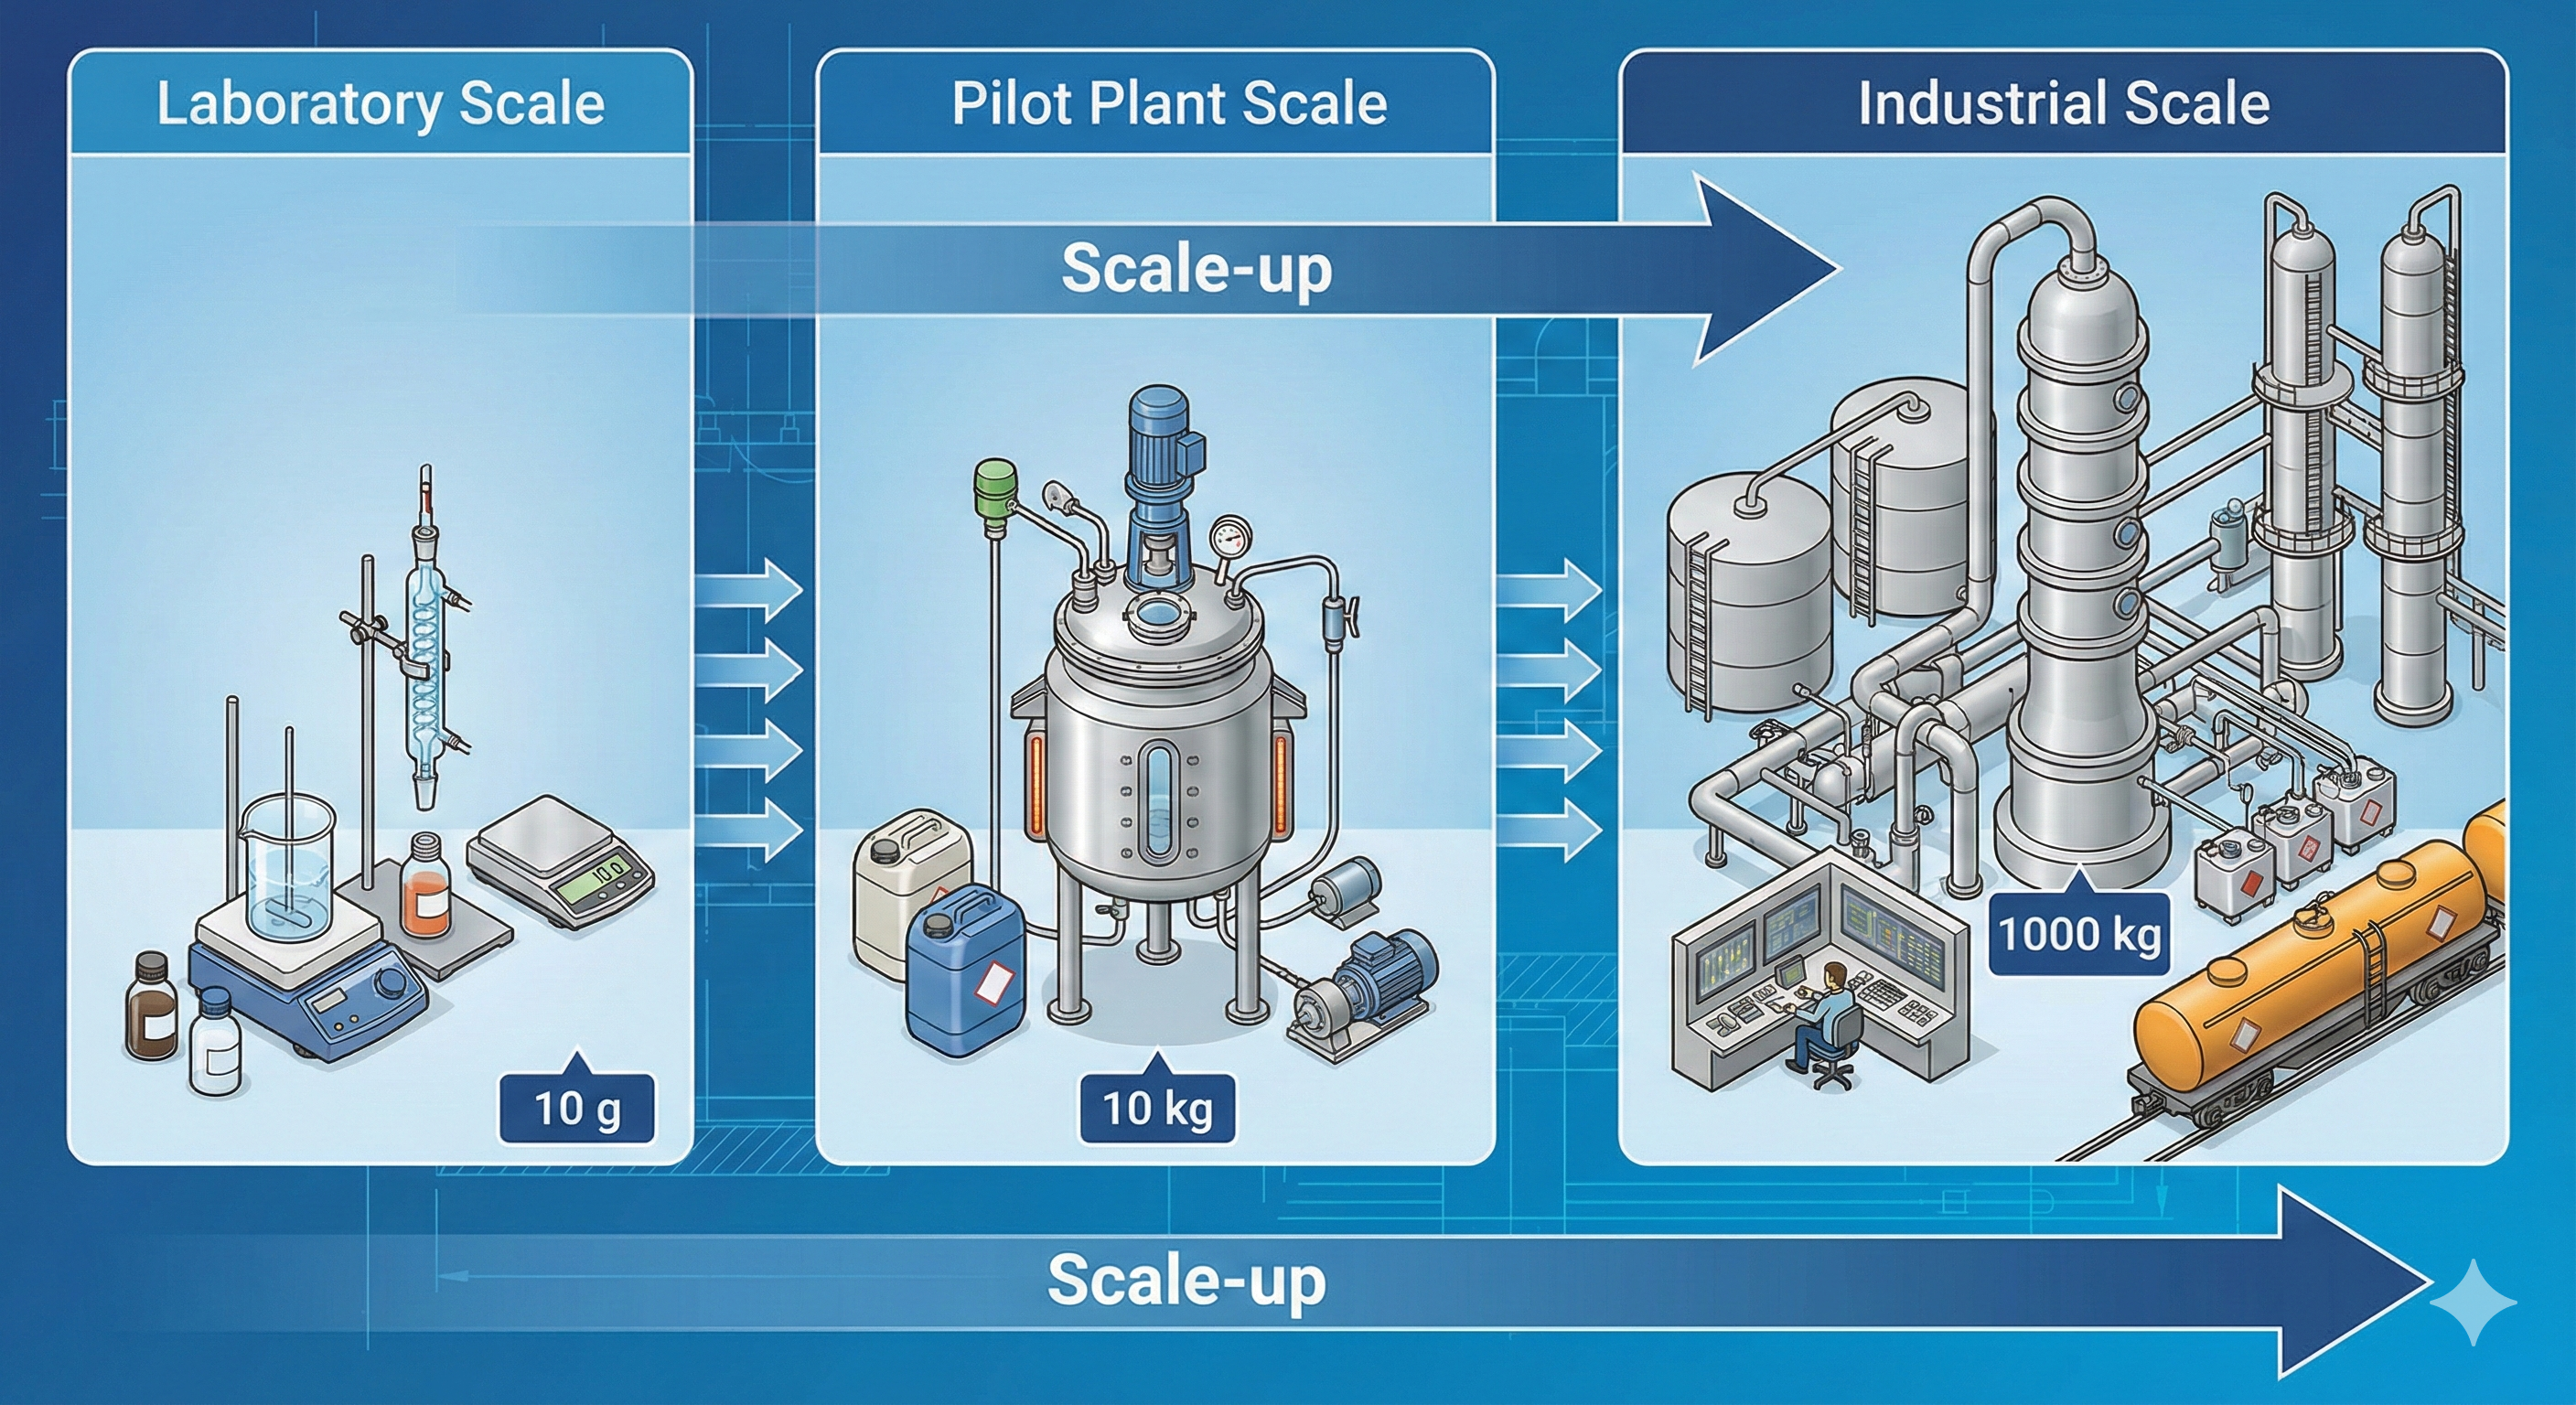
\includegraphics[width=6.36144in,height=2.22928in]{images/IntroToCHemEng2/media/image71.png}

\[A \rightarrow B\]

\hfill\break
נניח מצב עמיד, הפרדה מושלמת, וניקח בסיס חישוב של שעה.

\begin{enumerate}
\def\labelenumi{\arabic{enumi}.}
\setcounter{enumi}{5}
\tightlist
\item
  נעלמים - \(n_{A1},\ n_{A2},\ n_{B2},\ N_{B,out},\ n_{A,r}\) - סך הכל
  חמישה. נגדיר שתי מערכות ונחשב DOF על כל מערכת
\end{enumerate}

\textbf{מערכת 1: גבול מערכת על הריאקטור בלבד}

\textbf{נעלמים} \(\mathbf{N}_{\text{unknowns}}\) \textbf{-} לפי ההגדרה:
``נעלמים בזרמי הכניסה והיציאה בלבד'' (מה שחוצה את הגבול).
\({\dot{n}}_{A,1},\ {\dot{n}}_{A,2}\) \({\dot{n}}_{B,2}\) - שלושה
נעלמים.

\[N_{\text{unknowns}} = 3\]

\textbf{מספר תגובות בלתי תלויות} \(\mathbf{N}_{\text{reactions}}\)

תגובה אחת בלתי תלויה: \(N_{\text{reactions}} = 1\)**

\textbf{מספר מינים} \(\mathbf{N}_{\text{species}}\)

בגבול הריאקטור קיימים שני מינים: \(A,B\). לכן יש שני מאזני מינים:

\[N_{\text{species}} = 2\]

\textbf{קשרים נוספים} \(\mathbf{N}_{\text{other}}\)

נתון התהליך הוא ההמרה במעבר יחיד, והוא מוסיף קשר שאינו ``מאזן מין'':

\[X_{sp} = \frac{{\dot{n}}_{A,1} - {\dot{n}}_{A,2}}{{\dot{n}}_{A,1}} = 0.40\]

לכן:

\[N_{\text{other}} = 1\]

\textbf{חישוב DOF לריאקטור בלבד}

\[DOF = (N_{\text{unknowns}} + N_{\text{reactions}}) - N_{\text{species}} - N_{\text{other}} = (3 + 1) - 2 - 1 = 1\]

הריאקטור לבדו אינו סגור (חסר קשר אחד). זה הגיוני .
\({\dot{n}}_{A,1}\)נקבע על ידי לולאת התחזיר והמפריד, ולא על ידי הריאקטור
בלבד.

\textbf{חישוב DOF לנקודת הערבוב --}

\textbf{יש לנו 2 משתנים לא ידועים}
\(\mathbf{n}_{\mathbf{A,1}}\mathbf{,\ }\mathbf{n}_{\mathbf{A,r}}\)\textbf{,
ויש לנו משוואת מאזן מסה אחת על A}

\[DOF = (1 + 1) - 1 = 1\]

\textbf{חישוב DOF למפריד}

\textbf{יש לנו 4 משתנים לא ידועים.}
\(\mathbf{,\ }\mathbf{n}_{\mathbf{A2}}\mathbf{,\ }\mathbf{n}_{\mathbf{B2}}\mathbf{,\ }\mathbf{n}_{\mathbf{B,out}}\mathbf{,\ }\mathbf{n}_{\mathbf{A,r}}\)

\textbf{יש לנו שני מינים -- שני מאזני מסה.\\
ויש לנו שני אילוצים פיסיקליים שלא השתמשנו בהם -- העובדה שהזרם החוצה כולל
רק B, ושהזרם תחזיר כולל רק A}

\textbf{ולכן}\(\mathbf{DOF = 4 - 4 = 0}\)\textbf{.}

נתחיל עם המפריד

לפי שני מאזני המסה של המפריד אנחנו מקבלים:

\[n_{A2} = n_{A,r}\ \ \ ,\ \ \ n_{B2} = n_{B,out}\]

אמנם אנחנו עדיין לא יודעים בדיוק מה הערכים, אבל אנחנו בפועל מצמצמים שתי
דרגות חופש (כל שוויון מצמצם דרגה אחת)

נסתכל על נקודת הערבוב - \(n_{A_{f}} + n_{Ar} = n_{A1}\)

כעת נסתכל על הראקטור, תוך הצבת שני השוויונים שקיבלנו.

מתוך יחס ההמרה היחיד

\[X_{sp} = \frac{n_{A,1} - n_{A2}}{n_{A,1}} = 0.40 = > n_{A2} = 0.6n_{A,1}\ \]
ובעזרת נקודת הערבוב נוכל לחשב את כולם כל הזרמים של A

\[100kmol + n_{A2} = n_{A1}\]

\[n_{A2} = 0.6n_{A,1}\]

ולכן

\[100kmol + 0.6n_{A,1} = n_{A1}\]

\[n_{A1} = 250\ kmol\]

\[n_{Ar} = n_{A2} = 0.6*250\ kmol = 150\ kmol\]

ומתוך היחסים הסטויכיומטרים

\[n_{Acon} = n_{Bgen} = 100kmol\]

וכעת נחזור לבסיס החישוב של שעה אחת ונגדיר את הקצבים

\[{\dot{n}}_{A1} = 250\frac{kmol}{h}\ \ \ \ \ \ \ \ {\dot{n}}_{A2} = {\dot{n}}_{A,r} = 150\frac{kmol}{h}\ \ \ \ \ \ \ {\dot{n}}_{B2} = \ {\dot{n}}_{B,out} = 100\frac{kmol}{h}\ \]

\subsubsection{זרם סילוק/טיהור
Purge}\label{ux5d6ux5e8ux5dd-ux5e1ux5d9ux5dcux5d5ux5e7ux5d8ux5d9ux5d4ux5d5ux5e8-purge}

כאשר מפעילים תהליך עם \textbf{תחזיר אנו מ}חזירים לריאקטור חלק מזרם
היציאה כדי להעלות את הניצול הכולל של חומרי הגלם (במיוחד כש-\(X_{sp}\)
נמוך). אבל לרוב חומרי גלם כמעט אף פעם אינם טהורים: יש חומרים אינרטים
(למשל \(N_{2}\), \(Ar\), \(CO_{2}\)שלא מגיב, אדי מים), ולעיתים יש גם
\textbf{תוצרי לוואי} או מזהמים שנכנסים עם ההזנה או נוצרים בתהליך. אם
נפריד רק את התוצר ונחזיר את כל שאר הזרם הלא-מגיב חזרה לריאקטור, אותם
רכיבים לא רצויים ימשיכו להכנס למערכת אבל לא לצאת, ולכן הם ילכו ויצטברו
במחזור. ההצטברות משנה את הרכב זרם הכניסה לריאקטור, עלולה להפריע
לקינטיקה, להכביד על ההפרדה, ובמקרים מסוימים גם ליצור סיכוני בטיחות (למשל
הצטברות רכיב דליק/רעיל).

כאן נכנס \textbf{Purge} --

Purge או זרם סילוק/זרם טיהור - זהו זרם קטן שנלקח מתוך לולאת התחזיר ומוצא
החוצה מן המערכת. הרעיון פשוט: אם כל רכיב אינרטי שנכנס חייב גם לצאת בסוף,
ובמערכת עם תחזיר אין לו ``מסלול יציאה טבעי'', אנחנו \emph{מייצרים לו
מסלול יציאה} באמצעות Purge. בפועל Purge מוציא החוצה גם קצת מהמגיבים
היקרים, ולכן הוא תמיד פשרה בין שתי מגבלות: מצד אחד למנוע הצטברות אינרטים
ותוצרי לוואי, ומצד שני לא לאבד יותר מדי חומר גלם.

מבחינה תהליכית, נהוג להגדיר \textbf{שבר סילוק} (purge fraction) כלומר
איזה חלק מזרם המחזור מסולק:

\[f_{p} = \frac{{\dot{n}}_{P}}{{\dot{n}}_{\text{recycle loop}}}\]

ככל ש-\(f_{p}\) גדול יותר, האינרטים יוצאים מהר יותר וההצטברות קטנה, אבל
גדל גם איבוד המגיבים. ככל ש-\(f_{p}\) קטן יותר, נחסוך חומר גלם בטווח
הקצר אבל נסתכן בהצטברות שתפגע בביצועי התהליך .

מפעל לייצור מתנול (\(CH_{3}OH\)) מוזן בגז סינתזה המכיל פחמן חד-חמצני
(\(CO\)) ומימן (\(H_{2}\)). חומר הגלם מכיל גם כמות קטנה של מתאן
(\(CH_{4}\)), אשר אינו מגיב בתהליך (אינרטי). הריאקציה המתרחשת היא:\\
\[CO + 2H_{2} \rightarrow CH_{3}OH\]

הנתונים בתרשים, קצב הסילוק מכוונן כך שריכוז המתאן בכניסה לראקטור יהיה
10\% מולי

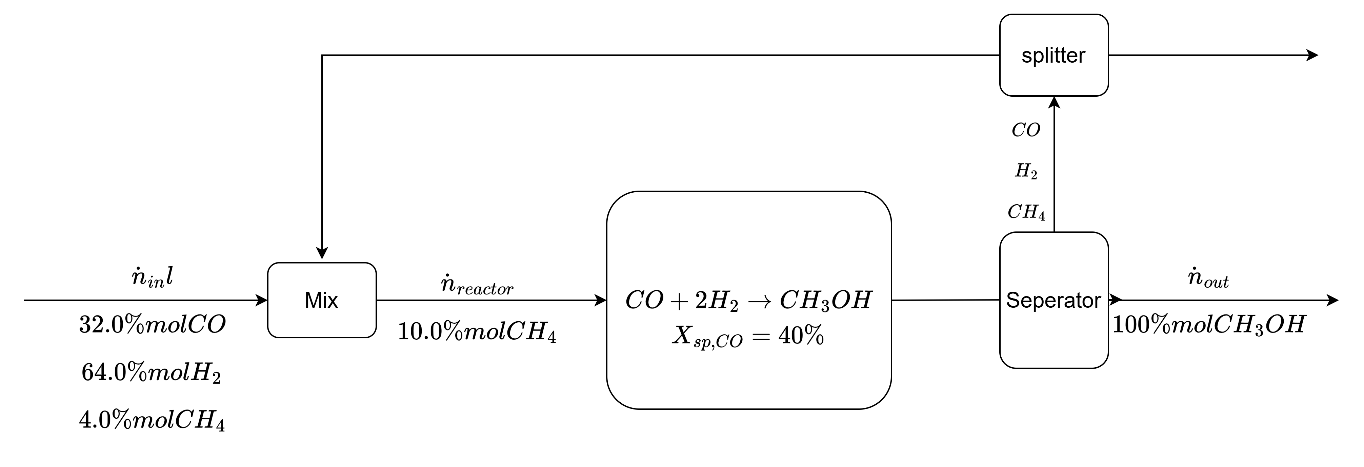
\includegraphics[width=6.18655in,height=2.11688in]{images/IntroToCHemEng2/media/image72.png}

מהי כמות המתנול אשר נוצרת בתהליך ומהו מקדם ההמרה הכללי?\\
מה צריך להיות התחזיר על מנת שהתהליך ישאר במצב עמיד?

פתרון

הנחות:

\begin{itemize}
\item
  הפרדה מושלמת במפריד. כל המתנול מתעבה ויוצא כתוצר טהור; כל הגזים
  \(CO,H_{2},CH_{4}\) יוצאים כזרם גז.
\item
  כל הזרמים הנכנסים והיוצאים מהמפצל הם בעלי אותו ההרכב.
\item
  כל האחוזים המוצגים בשרטוט הם מולריים
\end{itemize}

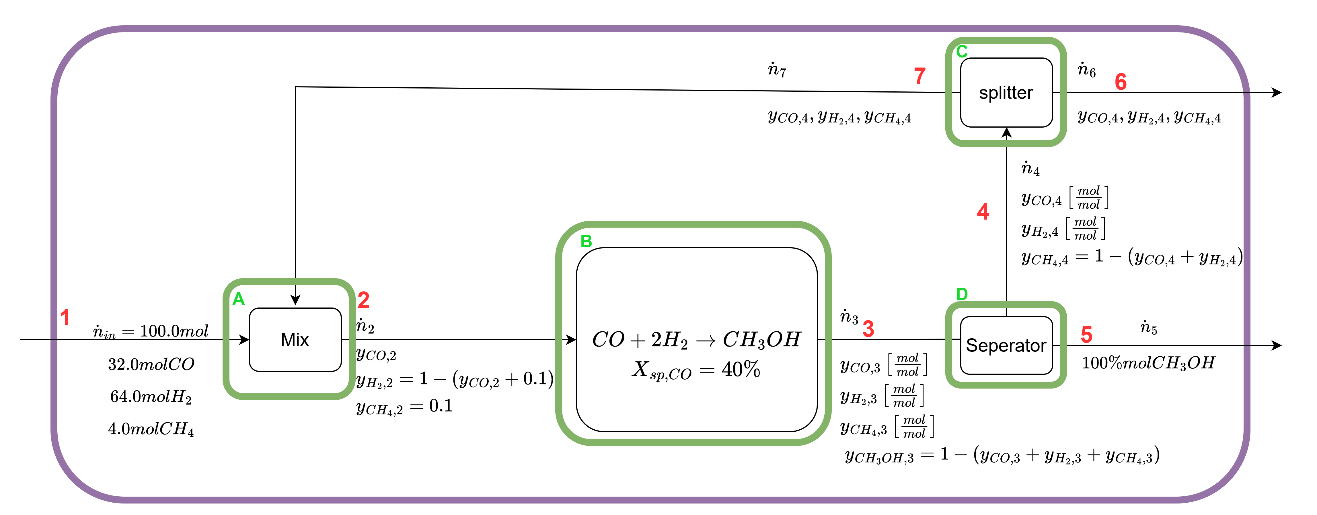
\includegraphics[width=5.96753in,height=2.33512in]{images/IntroToCHemEng2/media/image73.png}

\begin{quote}
\ul{נתחיל עם ניתוח דרגות חופש על המערכת הכוללת כ"קופסא שחורה" (ריבוע
סגול)}\\
מסתכלים רק על מה שנכנס ומה שיוצא

במערכת הכוללת יש לנו 3 זרמים -- 1,5,6\\
נחשב דרגות חופש על בסיס אטומים (כי יש לנו קופסא שחורה, אנחנו לא יודעים
מה קורה בפנים)\\
לכן חסרים 5 נעלמים
\(\ {\dot{n}}_{1},{\dot{n}}_{6},\ {\dot{n}}_{5},y_{CO,4},\ y_{H_{2},4}\ \)

ויש לנו 3 מאזנים אפשריים -- על שלושה אטומים C,H,O\(\ \)\\
ולכן דרגות חופש על המערכת הכוללת הן \(DOF = 5 - 3\) -- לא פתיר\\
נוכל להוריד דרגת חופש אחת על ידי הנחת בסיס חישוב של
\({\dot{n}}_{1} = \frac{100}{h}\) אבל עדיין חסרה עוד דרגה
\end{quote}

על מנת למצוא את המידע החסר נסתכל על תת המערכות השונות עם הנחת בסיס
החישוב\({\dot{n}}_{1} = \frac{100}{h}\)\\
עם הזמן תתפתח לנו האינטואיציה של אילו תת-מערכות עדיפות בכל סיטואציה ולא
באמת נחשב את דרגות החופש של כל תתי המערכות באופן מלא, אבל בשלב זה אנחנו
עדיין עושים זאת למען התרגול.

\begin{longtable}[]{@{}
  >{\raggedright\arraybackslash}p{(\linewidth - 8\tabcolsep) * \real{0.1360}}
  >{\raggedright\arraybackslash}p{(\linewidth - 8\tabcolsep) * \real{0.4560}}
  >{\raggedright\arraybackslash}p{(\linewidth - 8\tabcolsep) * \real{0.1760}}
  >{\raggedright\arraybackslash}p{(\linewidth - 8\tabcolsep) * \real{0.0960}}
  >{\raggedright\arraybackslash}p{(\linewidth - 8\tabcolsep) * \real{0.1120}}@{}}
\toprule\noalign{}
\begin{minipage}[b]{\linewidth}\raggedright
\begin{quote}
\textbf{תת־מערכת}
\end{quote}
\end{minipage} & \begin{minipage}[b]{\linewidth}\raggedright
\begin{quote}
\textbf{נעלמים}
\end{quote}
\end{minipage} & \begin{minipage}[b]{\linewidth}\raggedright
\begin{quote}
\textbf{מידע זמין (משוואות)}
\end{quote}
\end{minipage} & \begin{minipage}[b]{\linewidth}\raggedright
\begin{quote}
\textbf{DOF}
\end{quote}
\end{minipage} & \begin{minipage}[b]{\linewidth}\raggedright
\begin{quote}
\textbf{פתיר?}
\end{quote}
\end{minipage} \\
\midrule\noalign{}
\endhead
\bottomrule\noalign{}
\endlastfoot
\begin{minipage}[t]{\linewidth}\raggedright
\begin{quote}
מערכת כוללת (קופסה שחורה)
\end{quote}
\end{minipage} & \begin{minipage}[t]{\linewidth}\raggedright
\begin{quote}
\(\left( n_{3},n_{6},y_{CO,6},y_{CH_{4},6} \right)\)- סה"כ 4
\end{quote}
\end{minipage} & \begin{minipage}[t]{\linewidth}\raggedright
\begin{quote}
מאזנים אטומיים C,H,O -- סך הכל 3 מאזנים.
\end{quote}
\end{minipage} & \begin{minipage}[t]{\linewidth}\raggedright
\begin{quote}
1
\end{quote}
\end{minipage} & \begin{minipage}[t]{\linewidth}\raggedright
\begin{quote}
לא
\end{quote}
\end{minipage} \\
\begin{minipage}[t]{\linewidth}\raggedright
\begin{quote}
ערבוב (Mixer)
\end{quote}
\end{minipage} & \({\dot{n}}_{2},y_{CO,2},\)

\({\dot{n}}_{7},y_{CO,4},y_{CH_{4},4}\) &
\begin{minipage}[t]{\linewidth}\raggedright
\begin{quote}
מאזנים עם הרכיבים בנקודת הערבוב -- סך הכל 3 משוואות.
\end{quote}
\end{minipage} & \begin{minipage}[t]{\linewidth}\raggedright
\begin{quote}
2
\end{quote}
\end{minipage} & \begin{minipage}[t]{\linewidth}\raggedright
\begin{quote}
לא
\end{quote}
\end{minipage} \\
\begin{minipage}[t]{\linewidth}\raggedright
\begin{quote}
ריאקטור בלבד
\end{quote}
\end{minipage} & \begin{minipage}[t]{\linewidth}\raggedright
\begin{quote}
\[{{\dot{n}}_{2},y_{CO,2}
}{{\dot{n}}_{3},y_{CO,3},y_{H_{2},3},y_{CH_{4},3}}\]

משתנה תגובה (\(\xi\)) - סה"כ 7
\end{quote}
\end{minipage} & \begin{minipage}[t]{\linewidth}\raggedright
\begin{quote}
משוואות על מינים מוגדרות באמצעות \(\xi\) -- 4 משוואות\\
אילוצים פיסיקליים -- מקדם המרה\\
סך הכל - 5
\end{quote}\strut
\end{minipage} & \begin{minipage}[t]{\linewidth}\raggedright
\begin{quote}
2
\end{quote}
\end{minipage} & \begin{minipage}[t]{\linewidth}\raggedright
\begin{quote}
לא
\end{quote}
\end{minipage} \\
\begin{minipage}[t]{\linewidth}\raggedright
\begin{quote}
מפריד (Condenser) בלבד
\end{quote}
\end{minipage} & \begin{minipage}[t]{\linewidth}\raggedright
\begin{quote}
\[{\dot{n}}_{3},y_{CO,3},y_{H_{2},3},y_{CH_{4},3}\]

\[{\dot{n}}_{4},y_{CO,4},y_{CH_{4},4}\]

\[{\dot{n}}_{5}\]
\end{quote}
\end{minipage} & \begin{minipage}[t]{\linewidth}\raggedright
\begin{quote}
4 מאזנים על 4 רכיבים
\end{quote}
\end{minipage} & \begin{minipage}[t]{\linewidth}\raggedright
\begin{quote}
4
\end{quote}
\end{minipage} & \begin{minipage}[t]{\linewidth}\raggedright
\begin{quote}
לא
\end{quote}
\end{minipage} \\
\begin{minipage}[t]{\linewidth}\raggedright
\begin{quote}
מפצל (Splitter) בלבד
\end{quote}
\end{minipage} & \begin{minipage}[t]{\linewidth}\raggedright
\begin{quote}
\[{\dot{n}}_{4},{\dot{n}}_{7},{\dot{n}}_{6}\]
\end{quote}
\end{minipage} & \begin{minipage}[t]{\linewidth}\raggedright
\begin{quote}
מאזן מסה על הספיקות\\
(אין טעם לעשות על הרכיבים, כולם נגזרים מהיחס בין הספיקות)
\end{quote}\strut
\end{minipage} & \begin{minipage}[t]{\linewidth}\raggedright
\begin{quote}
4
\end{quote}
\end{minipage} & \begin{minipage}[t]{\linewidth}\raggedright
\begin{quote}
לא
\end{quote}
\end{minipage} \\
\end{longtable}

\begin{quote}
ובשלב ראשון אנחנו רואים שאין לנו שום תת מערכת, אבל התת מערכת הכי קרובה
לפתרון היא תת מערכת על הראקטור, ולכן ננסה לפתח אותה יותר לעומק. האם נוכל
למצוא מידע נוסף?
\end{quote}

\begin{itemize}
\tightlist
\item
  ישנו אילוץ נוסף על המערכת שלא שמנו לב אליו כי הוא דורש תנאים
  ספציפיים.- אם נסתכל על היחס בין הCO למימן אנחנו רואים שהיחס בכניסה הוא
  1:2, וגם יחס התגובה הוא 1:2. מאחר ובשום מקום אנחנו לא מפרידים בינהם,
  והם תמיד ממשיכים יחד באותם הזרמים המשמעות היא שהיחס בינהם בכל הזרמים
  חייב להיות בהכרח
\end{itemize}

\[\frac{n_{CO}}{n_{H_{2}}} = \frac{y_{CO}}{y_{H_{2}}} = \frac{1}{2}\]

\begin{itemize}
\tightlist
\item
  אמנם אין אפשרות לפתור את הראקטור באופן מלא, אבל אנחנו יכולים לפתור רק
  חלק מהמשתנים אם נתמקד בתכונות האינטנסיביות של הראקטור, וננסה לחשב רק
  את ההרכבים של הזרמים. לצורך כך נוכל להגדיר \ul{בסיס חישוב זמני} רק
  עבור הראקטור שיהיה נוח לחישוב
\end{itemize}

\begin{quote}
\[{\dot{n}}_{2}^{*} = 100\frac{mol}{h}\]
\end{quote}

מאחר שכל הזרמים בלולאה (יציאה מהראקטור, זרם הגז לאחר ההפרדה, זרם התחזיר
וזרם הסילוק) \textbf{קשורים זה לזה ליניארית}, שינוי קנה המידה של הספיקה
משנה רק את הערכים המוחלטים -- אך \textbf{אינו משנה את השברים המולריים}
.אמנם הערכים \({\dot{n}}_{2}^{*},{\dot{n}}_{3}^{*}\) לא יהיו נכונים עבור
המערכת הגדולה, אבל זה יאפשר לנו למצוא את ההרכבים.
\(y_{H_{2,3}}\ ,\ y_{CO_{3}},\ y_{{CH}_{4,3}},y_{{CH}_{4,3}}\)\\

בחירת בסיס חישוב זמני (כמו \(\dot{n} = 100\)) \textbf{לצורך מציאת
הרכבים} מותרת רק כאשר המידע הזמין קובע יחסים בין זרמים, אך לא קובע את
הסקאלה המוחלטת שלהם.

מתי נוכל להגדיר בסיס חישוב זמני? מספר דוגמאות:

\begin{enumerate}
\def\labelenumi{\arabic{enumi}.}
\item
  ריאקטור עם המרה נתונה, כאשר ספיקת הכניסה אינה ידועה. במקרה זה
  הסטויכיומטריה וההמרה קובעות את היחסים בין המינים, אך לא את הספיקה
  הכוללת.
\item
  לולאת תחזיר עם אילוץ על הרכב (למשל ריכוז אינרטי בכניסה לריאקטור).
  האילוץ קובע את ההרכב בלולאה, אך הסקאלה נקבעת רק במאזן הגלובלי.
\end{enumerate}

מתי לא נוכל להגדיר בסיס חישוב זמני? דוגמאות

\begin{enumerate}
\def\labelenumi{\arabic{enumi}.}
\item
  מערכת שבה ספיקת ההזנה נתונה במפורש (למשל \(100\text{ kmol/h}\)). במקרה
  זה הסקאלה כבר נקבעה, ואין חופש לבחור בסיס אחר.
\item
  בעיות הכוללות קינטיקה או מאזני אנרגיה התלויים בריכוזים או בספיקות
  מוחלטות. כאן שינוי הבסיס משנה את הפיזיקה של הבעיה, ולא רק את המספרים.
\end{enumerate}

או בקיצור

\textbf{בסיס חישוב זמני מותר רק כאשר הבעיה עדיין לא קבעה סקאלה.\\
אם הסקאלה נקבעה -- אין חופש לבחור בסיס.}

\begin{quote}
עם המידע הנוסף ננסה לפתור את המערכת\\
משוואת המרה -
\(\frac{{\dot{n}}_{CO,2} - {\dot{n}}_{CO,3}}{{\dot{n}}_{CO,2}} = 0.40\)**
\ul{אילוץ בכניסה לראקטור שנקבע על ידי התהליך} \(y_{CH_{4},2} = 0.10\)

ובסיס חישוב זמני ** \[{\dot{n}}_{2}^{*} = 100\frac{mol}{h}\]

\{מבחינה רעיונית אנחנו מנתחים עכשיו מערכת אחרת שהספיקה בכניסה שלה היא
שונה, והספיקה בכניסה לראקטור היא \(n_{1}^{*}\) במקרה זה לא תהיה 100mol
אבל היחסים בין הזרמים חייבים להשמר ולכן השברים המולריים עבור המערכת הזו
יהיה זהה לחישוב היחסים עבור המערכת השנייה\}

מהאילוץ:

\[n_{CH_{4},2}^{*} = {\dot{n}}_{2}^{*}{\ y}_{CH_{4},2}\ \ \ \ y_{CH_{4},2} = 0.10\frac{mol}{mol}\]

\[\Rightarrow n_{CH_{4},2}^{*} = 100\frac{mol}{h}*0.10\frac{mol}{mol} = 10\frac{mol}{h}\]

לכן:

\[{\dot{n}}_{2}^{*} = {\dot{n}}_{CO,2}^{*} + {\dot{n}}_{H_{2},2}^{*} + n_{CH_{4},2}^{*}\]

\[{\dot{n}}_{CO,2}^{*} + {\dot{n}}_{H_{2},2}^{*} = 90\frac{mol}{h}\]

נשתמש ביחס בין המימן לCO

\[\frac{n{\dot{\text{ }}}_{H_{2,2}}^{*}}{{\dot{n}}_{CO,2}^{*}} = \frac{2}{1}\ \  \Longrightarrow \ \ \ {\dot{n}}_{H_{2},2}^{*} = 2{\dot{n}}_{CO,2}^{*}\]

ולכן

\[{\dot{n}}_{CO,2}^{*} + 2{\dot{n}}_{CO,2}^{*} = 90\frac{mol}{h}\]

\[{\dot{n}}_{CO,2}^{*} = 30\frac{mol}{h},\ \ \ \ \ \ \ \ \ \ \ {\dot{n}}_{H_{2},2}^{*} = 60\frac{mol}{h}\]

\[y_{CO,2}^{*} = 0.3,\ \ \ \ \ \ \ \ \ \ \ y_{H_{2},2}^{*} = 0.6\frac{mol}{h}\]

כעת נשתמש במקדם ההמרה \(X_{sp,CO} = 0.40\):

\[X_{sp,CO} = \frac{{\dot{n}}_{CO,2}^{*} - {\dot{n}}_{CO,3}^{*}}{{\dot{n}}_{CO,2}^{*}}\  = > \ {\dot{n}}_{CO,3}^{*} = {\dot{n}}_{CO,2}^{*}\left( 1 - X_{SP} \right)\ \]

\[\ {\dot{N}}_{CO,3}^{*} = {\dot{n}}_{CO,2}^{*}\left( 1 - X_{SP} \right)\]

\[{\dot{n}}_{CO,3}^{*} = 30\frac{mol}{h}(1 - 0.4) = 18\frac{mol}{h}\]
ושוב לפי יחס המגיבים

\[{\dot{n}}_{H_{2},3}^{*} = 2{\dot{n}}_{CO,3}^{*}\ \ \ \  = > {\dot{n}}_{H_{2},3}^{*} = 2*18\frac{mol}{h} = 36\frac{mol}{h}\ \ \ \ \]

כמות החומר האינרטי לא משתנה:

\[{\dot{n^{*}}}_{CH_{4},3} = 10\]

ונוצר מתנול לפי היחסים הסטויכיומטרים --

\[\frac{\nu_{CH_{3}OH,3}}{\nu_{CO,reacted}} = \frac{{\dot{n}}_{CH_{3}OH,3}}{{\dot{n}}_{CO,2}^{*}X_{SP}}\]

\[{\dot{n}}_{CH_{3}OH,3} = \frac{\nu_{CH_{3}OH,3}}{\nu_{CO,reacted}}{\dot{n}}_{CO,2}^{*}X_{SP} = \frac{1}{1}*30\frac{mol}{h}*0.4 = 12\frac{mol}{h}\]

\[{{\dot{n}}^{*}}_{CH_{3}OH,3} = 12\frac{mol}{h}\] כעת אנחנו יודעים את
הכמויות של כל החומרים ביציאה מהראקטור ולכן ניתן לחשב את השברים המוליים
שלהם

\[{\dot{n}}_{3}^{*} = {\dot{n}}_{CO,3}^{*} + {\dot{n}}_{H_{2},3}^{*} + n_{CH_{4},3}^{*} + {\dot{n}}_{CH_{3}OH,3}^{*}\]

\[{\dot{n}}_{3}^{*} = 18\frac{mol}{h} + 36\frac{mol}{h} + 10\frac{mol}{h} + 12\frac{mol}{h} = 76\frac{mol}{h}\]

\[{y_{CH_{4},3} = \frac{10\frac{mol}{h}}{76\frac{mol}{h}} = 0.13
}{y_{CO,3} = \frac{18\frac{mol}{h}}{76\frac{mol}{h}} = 0.24
}{y_{H_{2},3} = \frac{36\frac{mol}{h}}{76\frac{mol}{h}} = 0.47}\]

\[y_{CH_{3}OH,3} = \frac{12\frac{mol}{h}}{76\frac{mol}{h}} = 0.16\]
\end{quote}

ומצאנו את היחסים המולריים ביציאה מהראקטור

מאחר והמפריד יוצר הפרדה מלאה, וכל המתנול ממשיך לצד אחד, ושאר הגזים לזרם
אחר, אנו יכולים למצוא גם את הרכב הגזים בזרם 4

\begin{quote}
\[{y_{CH_{4},4} = \frac{10\frac{mol}{h}}{(76 - 12)\frac{mol}{h}} = 0.16
}{y_{CO,4} = \frac{18\frac{mol}{h}}{(76 - 12)\frac{mol}{h}} = 0.28
}{y_{H_{2},4} = \frac{36\frac{mol}{h}}{(76 - 12)\frac{mol}{h}} = 0.56}\]
\end{quote}

(אם רוצים לראות את זה באופן פורמלי אפשר לבנות את המאזנים המפריד על אותו
בסיס חישוב זמני, או לחילופין להחליט מלכתחילה שעושים את כל החישובים על תת
מערכת המכילה את הראקטור והמפריד. עם הזמן נדע לזהות זרמים כמו זרם 3
שמוסיפים לנו המון משתנים למערכת ומעט מאוד מידע, ולכן לבחור תת מערכות
המכילות בתוכן את הזרמים הללו).

\begin{quote}
חשוב לשים לב שגם כאן כל הערכים המוחלטים מתבססים על בסיס החישוב הזמני
שלנו \({\dot{n}}^{*}\), ולכן נשתמש רק ביחסים ולא בערכים המוחלטים כשנחזור
למערכת המלאה.

כעת נסתכל על המערכת הכוללת עם בסיס חישוב
\(\dot{n_{1}} = 100\frac{mol}{h}\)\\
ועם היחסים\\
\[y_{CH_{4},4} = 0.16,\ \ \ \ y_{CO,4} = 0.28,\ \ \ \ \ y_{H_{2},4} = 0.56\]
\end{quote}

ונשארו לנו רק שני נעלמים \(\dot{n_{5},}\ \dot{n_{6}}\)

\begin{quote}
\ul{מאזן על המתאן}

\({\dot{n}}_{CH_{4},1} = {\dot{n}}_{6}*y_{CH_{4},6}\)

\{ אם אנחנו במצב עמיד אז כל המתאן שנכנס חייב לצאת בזרם הטיהור (אחרת תהיה
הצטברות).\}

\(4.0\frac{mol}{h} = {\dot{n}}_{6}*0.16\  \Rightarrow \ {\dot{n}}_{6} = 25.0\frac{mol}{h}\)
\end{quote}

ומספר המולים הכללי בזרם 6 יהיה שווה גם ל-

\[{\dot{n}}_{6} = {\dot{n}}_{CH_{4},6} + {\dot{n}}_{H_{2},6} + {\dot{n}}_{CO,6}\]

נזכור שקיים יחס קבוע בין
\[\frac{n_{CO}}{n_{H_{2}}} = \frac{y_{CO}}{y_{H_{2}}} = \frac{1}{2}\]

\[25.0\frac{mol}{h} = 4.0\frac{mol}{h} + 2{\dot{n}}_{CO,6} + {\dot{n}}_{CO,6}\]

\[{\dot{n}}_{CO,6} = 7.0\frac{mol}{h}\ \ \ \ ,\ \ \ {\dot{n}}_{H_{2},6} = 14.0\frac{mol}{h}\ \ \]

נעצור ונזכר מה שאלו אותנו

מהי כמות המתנול אשר נוצרת בתהליך ומהו מקדם ההמרה הכללי?\\
מה צריך להיות התחזיר על מנת שהתהליך ישאר במצב עמיד?

\begin{quote}
\ul{מאזן על ה CO}

\[{\dot{n}}_{in} = {\dot{n}}_{reacted} + {\dot{n}}_{out}\]

\[{\dot{n}}_{CO,1} = {\dot{n}}_{co,reacted} + {\dot{n}}_{CO,6}\]

\[32\frac{mol}{h} = {\dot{n}}_{co,reacted} + 7\frac{mol}{h}\ \  \Rightarrow \ {\dot{n}}_{co,reacted} = 25\frac{mol}{h}\]

ולכן מקדם ההמרה הכללי יהיה
\(X_{ov} = \frac{{\dot{n}}_{CO,1} - {\dot{n}}_{CO,6}}{{\dot{n}}_{CO,1}}\)

\[X_{ov} = \frac{32\frac{mol}{h} - 7\frac{mol}{h}}{32\frac{mol}{h}} = 0.78\ או\ \ 78\%\]

\ul{מאזן על המתנול}

\[{\dot{n}}_{in} + {\dot{n}}_{generated} = {\dot{n}}_{out}\]

\[{\dot{n}}_{CH_{3}OH,gen} = \frac{\nu_{CH_{3}OH}}{\nu_{CO}}{\dot{n}}_{co,reacted}\]

\[{\dot{n}}_{CH_{3}OH,gen} = \frac{1}{1}*25\frac{mol}{h} = 25\frac{mol}{h}\]

על מנת למצוא את התחזיר נצטרך להשתמש בנתונים מתוך הלולאה\\
נזכר ביחסים שמצאנו **
\[y_{CO,2}^{} = 0.3,\ \ \ \ \ \ \ \ \ \ \ y_{H_{2},2}^{} = 0.6\frac{mol}{h}\]

\[y_{CH_{4},4} = 0.16,\ \ \ \ y_{CO,4} = 0.28,\ \ \ \ \ y_{H_{2},4} = 0.56\]

\[{\dot{n}}_{CO,6} = 7.0\frac{mol}{h}\ \ \ \ ,\ \ \ {\dot{n}}_{H_{2},6} = 14.0\frac{mol}{h}\]

ומתוך המאזן על נקודת הערבוב

אין תגובה אז מספר המולים שנכנס חייב להיות שווה למספר המולים שיוצא

\[{\dot{n}}_{in} + {\dot{n}}_{7} = {\dot{n}}_{2}\]

מאזנים על הCO

\[{\dot{n}}_{CO,in} + {\dot{n}}_{CO,7} = {\dot{n}}_{CO,2} \Rightarrow 32\frac{mol}{h} + 0.28{\dot{n}}_{7} = 0.3{\dot{n}}_{2}\]

\[100\frac{mol}{h} + {\dot{n}}_{7} = {\dot{n}}_{2}\]

\[32\frac{mol}{h} + 0.28{\dot{n}}_{7} = 0.3{\dot{n}}_{2}\]

נחלק משוואות

\[\frac{32\frac{mol}{h} + 0.28{\dot{n}}_{7}}{100\frac{mol}{h} + {\dot{n}}_{7}} = 0.3\]

\[32\frac{mol}{h} + 0.28{\dot{n}}_{7} = 30\frac{mol}{h} + 0.3{\dot{n}}_{7}\]

\[2\frac{mol}{h} = 0.02{\dot{n}}_{7}\  \Rightarrow \ {\dot{n}}_{7} = 100\frac{mol}{h}\]

\[{\dot{n}}_{in} + {\dot{n}}_{7} = {\dot{n}}_{2} = 100\frac{mol}{h} + 100\frac{mol}{h} = 200\frac{mol}{h}\]

נבדוק את עצמינו עם מאזן על המתאן

\[{\dot{n}}_{in,CH_{4}} + {\dot{n}}_{7}y_{CH_{4},4} = {\dot{n}}_{2}y_{CH_{4},2}\]

\[4\frac{mol}{h} + 100\frac{mol}{h}0.16\overset{?}{\overbrace{=}}200\frac{mol}{h}*0.1\]
\end{quote}

ורואים שהמאזן מתקיים.

התחזיר הוא למעשה זרם 7 \[{\dot{n}}_{7} = 100\frac{mol}{h}\]

\subsection{סיכום -- מאזנים במערכות הכוללות
תגובות}\label{ux5e1ux5d9ux5dbux5d5ux5dd-ux5deux5d0ux5d6ux5e0ux5d9ux5dd-ux5d1ux5deux5e2ux5e8ux5dbux5d5ux5ea-ux5d4ux5dbux5d5ux5dcux5dcux5d5ux5ea-ux5eaux5d2ux5d5ux5d1ux5d5ux5ea}

במערכות ללא ריאקציה, הכלל המנחה הוא \(Input\  = \ Output\) אך כאשר
מתרחשת תגובה כימית, מולקולות נצרכות ונוצרות, ולכן כלל זה אינו תקף עוד
עבור המולקולות (אך נותר תקף עבור האטומים). בפרק זה הוצגו שלוש גישות
לפתרון בעיות ומערכת מושגים לניתוח תהליכים מורכבים.

\begin{itemize}
\item
  \textbf{מאזן מולקולרי (Molecular Balance):}

  \begin{itemize}
  \item
    \textbf{העיקרון:} התחשבות בשינוי הכימי באמצעות איברי יצירה וצריכה.\\
    נשתמש במשוואה \(In\  + \ Gen\  = \ Out\  + \ Con\)עבור כל מין כימי.
  \item
    איברי היצירה והצריכה מחושבים באופן ישיר על בסיס היחסים הסטויכיומטרים
    בתגובה.
  \item
    זו השיטה הכי אינטואיטיבית, אך היא הכי רגישה לטעויות חישוב וטעויות
    סימון, ולכן לרוב מתאים למערכות פשוטות עם ריאקציה בודדת.
  \end{itemize}
\item
  \textbf{מאזן אטומי (Atomic Balance):}

  \begin{itemize}
  \item
    \textbf{העיקרון:} אטומים אינם נוצרים או נעלמים. מתייחסים למערכת
    כ"קופסה שחורה" וסופרים אטומים בלבד. נשתמש במשוואה
    \(Input\  = \ Output\) עבור כל סוג אטום.
  \item
    השיטה המהירה ביותר למציאת זרמי יציאה (למשל בתהליכי שריפה), חוסכת
    חישובי ביניים אך לא מספקת מידע על הריאקציה עצמה.
  \end{itemize}
\item
  \textbf{מידת ההתקדמות (Extent of Reaction -}
  \(\mathbf{\xi}\)\textbf{):}

  \begin{itemize}
  \item
    \textbf{העיקרון:} שימוש במשתנה \(\xi\) המייצג את מספר הפעמים
    שהריאקציה התרחשה ("המנוע הפנימי"). כל השינויים במולי המגיבים
    והתוצרים מבוטאים באמצעות \(\xi\) והמקדמים הסטוכיומטריים
    \(n_{out} = n_{in} + \nu\xi\)
  \item
    פתרון עקבי ואחיד, המבוסס על משתנה מרכזי אחד עבור כל ראקציה. מועדפת
    כאשר ישנן מספר ריאקציות במקביל או בשימוש בתוכנות מחשב.
  \end{itemize}
\end{itemize}

\textbf{\ul{דרגות חופש (DOF) במערכות עם ריאקציה}}

יש שתי דרכים לחשב דרגות חופש במערכות עם ראקציה. בכל מקרה יש להקפיד לספור
רק \textbf{ריאקציות בלתי תלויות} (ריאקציות שלא ניתן להרכיב כקומבינציה
לינארית של ריאקציות אחרות).

\begin{itemize}
\tightlist
\item
  בגישת המאזן האטומי:
\end{itemize}

\[DOF = N_{unknowns} - N_{atomic\text{\_}balances} - N_{molecular\text{\_}inerts} - N_{other}\]

האטומים שהם חלק מהתגובה נספרים בנפרד, חומרים אינרטים מקבלים משוואה נפרדת

\begin{itemize}
\tightlist
\item
  בגישת מידת ההתקדמות / מאזן מולקולרי:
\end{itemize}

\[DOF = \left( N_{unknowns} + N_{reactions} \right) - N_{species} - N_{other}\]

סופרים את כל המינים כמשוואות, ומוסיפים נעלמים עבור כל ריאקציה.

בכל המקרים צריך לשים לב -- את האילוצים הפיסיקליים נספור רק כאשר הם
כוללים את הנעלמים שבמערכת/תת מערכת אותה אנחנו מנסים לפתור, ולא מוסיפים
לנו נעלמים חדשים.

\textbf{מערכות מורכבות -- תחזיר (Recycle) וזרם סילוק (Purge).}

בתעשייה המרה מלאה נדירה ולכן משתמשים במבנה תהליכי המאפשר ניצול יעיל של
משאבים:

\begin{itemize}
\item
  \textbf{תחזיר (Recycle):} החזרת חומרי גלם שלא הגיבו לריאקטור לטובת
  ניצול חוזר.
\item
  \textbf{הגדרות המרה:}

  \begin{itemize}
  \item
    \textbf{המרה במעבר יחיד (}\(\mathbf{X}_{\mathbf{sp}}\)\textbf{):}
    יעילות הריאקטור עצמו ("מה נצרך בריאקטור חלקי מה שנכנס אליו").
  \item
    \textbf{המרה כוללת (}\(\mathbf{X}_{\mathbf{ov}}\)\textbf{):} יעילות
    התהליך כולו ("מה נצרך במערכת חלקי מה שקנינו כחומר גלם טרי").
  \end{itemize}
\item
  \textbf{זרם סילוק (Purge)} נדרש כאשר חומרי הגלם מכילים אי-ניקיונות
  (אינרטים). ללא זרם הסילוק האינרטים יצטברו בלולאת המחזור.זרם הסילוק הוא
  פשרה בין הוצאת אינרטים לאובדן חומר גלם.
\end{itemize}

\textbf{טכניקות פתרון מתקדמות}

\begin{itemize}
\item
  \textbf{בסיס חישוב זמני:} בתת-מערכות (כמו לולאת מחזור) בהן ידועים יחסי
  הזרמים וההרכבים אך לא הספיקה המוחלטת, ניתן להניח בסיס חישוב שרירותי
  (למשל \(100\) מול), לחשב את ההרכבים (\(y_{i}\)) ואז לחזור למערכת המלאה
  ולהשתמש ביחסים שנמצאו.
\item
  \textbf{בחירת תת-מערכת:} ככל שהמערכת מורכבת יותר יש יותר חשיבות בבחירת
  מסלול הפתרון הנכון -- קופסא שחורה, מערכת כוללת, וחלוקה לתת מערכות
  שונות. הערכה נכונה של DOF תעזור לנו למצוא את המסלול המהיר ביותר.
\end{itemize}

\section{תגובות
שריפה}\label{ux5eaux5d2ux5d5ux5d1ux5d5ux5ea-ux5e9ux5e8ux5d9ux5e4ux5d4}

תגובות שריפה הן מהתגובות הכימיות המוכרות והאינטואיטיביות ביותר: כולנו
יודעים שדלק ``נשרף'', שדרוש חמצן, ושמתקבלים חום וגזי פליטה, אך מעבר לכך
תגובות שריפה הן אולי הסוג הנפוץ והחשוב ביותר של תגובות כימיות בתעשייה.
יש סוגים רבים של תגובות שריפה אך כולן מתבססות על אותו העקרון

תגובת שריפה - תגובה מהירה בין \textbf{דלק} (Fuel) לבין \textbf{מחמצן}
(Oxidizer) המשחררת כמות גדולה של אנרגיה.

מנקודת מבט של הנדסת תהליכים, שריפה היא מקרה פרטי ומאוד שימושי של תגובה
כימית. מבחינת מהנדס התהליך, שריפה היא "רק" עוד תגובה כימית, וכל חוקי
מאזני החומר שלמדנו (כולל מגיב מגביל, המרה וסטויכיומטריה) חלים גם כאן
בדיוק באותו אופן. עם זאת, בגלל השכיחות העצומה וההיסטורית של התהליכים
הללו, התפתח עבורם ז\textquotesingle רגון מקצועי ייחודי. מסיבה זו, תגובות
שריפה משמשות מודל קלאסי ללימוד ולתרגול של מושגי יסוד בניתוח מערכות עם
תגובות כימיות.

\subsection{מושגי
היסוד}\label{ux5deux5d5ux5e9ux5d2ux5d9-ux5d4ux5d9ux5e1ux5d5ux5d3}

\subsubsection{הדלק (Fuel)}\label{ux5d4ux5d3ux5dcux5e7-fuel}

הדלק הוא חומר הגלם אותו אנו שורפים במטרה להפיק אנרגיה תרמית. מבחינה
כימית, רוב הדלקים התעשייתיים הם \textbf{פחמימנים} (Hydrocarbons) -
תרכובות אורגניות הבנויות בעיקר מאטומי פחמן (C) ומימן (H). האנרגיה הרבה
המשתחררת בתהליך השריפה נובעת מפירוק הקשרים הכימיים במולקולות הדלק ויצירת
קשרים חדשים ויציבים יותר עם החמצן.

נהוג לסווג את הדלקים לפי מצב הצבירה שלהם, שכן הוא מכתיב את אופן הטיפול
בהם ואת הציוד ההנדסי הנדרש. \textbf{דלקים גזיים}, ובראשם הגז הטבעי
(Natural Gas), הם הנפוצים והנקיים יחסית. במודלים פשוטים נהוג להתייחס לגז
טבעי כאל מתאן טהור (\({CH}_{4}\)( בפועל הוא מכיל תערובת של פחמימנים קלים
נוספים (כגון אתאן ופרופאן) ולעיתים גם גזים שאינם דליקים. \textbf{דלקים
נוזליים}, כמו הבנזין, הסולר והמזוט, הם תוצרי זיקוק של נפט גולמי. דלקים
אלו הם תערובות מורכבות של מאות סוגי מולקולות, ולכן בחישובי הנדסה נהוג
לייצג אותם באמצעות נוסחה כימית "ממוצעת" או באמצעות הרכב משקלי
(\(wt\%\)). הקבוצה השלישית היא \textbf{דלקים מוצקים,} כאשר הנציג הבולט
הוא הפחם (Coal) המורכב ברובו מפחמן.

חשוב לזכור כי בניגוד למתרחש במעבדה הסטרילית או בתרגילי הכימיה
התיאורטיים, הדלקים במציאות התעשייתית אינם טהורים. הם מכילים רכיבים
נוספים ("אי-ניקיונות") המשפיעים מהותית על תהליך השריפה ועל חישובי המאזן.
הזיהום המשמעותי ביותר הוא הגופרית (S), המצויה באופן טבעי בנפט ובפחם.
בתהליך השריפה, הגופרית מתנהגת באופן דומה לפחמן -- היא מתרכבת עם החמצן
ונשרפת על פי המשוואה:

\[S + O_{2} \rightarrow SO_{2}\]

התוצר, גופרית דו-חמצנית (\(SO_{2}\)), הוא גז רעיל המהווה מקור זיהום
סביבתי חמור (גשם חומצי). מבחינת מהנדס התהליך, נוכחות גופרית מחייבת
התייחסות כפולה: ראשית, הגופרית צורכת חמצן ולכן משפיעה על כמות האוויר שיש
להזין למערכת; ושנית, יש לקחת בחשבון את הטיפול בתוצרי הלוואי הנוצרים.

מלבד הגופרית, דלקים (ובמיוחד פחם) מכילים לרוב גם \textbf{אפר} (Ash) -
מינרלים ומתכות שאינם משתתפים בתגובה הכימית, נכנסים ויוצאים מהמערכת
כמוצק, ומהווים פסולת שיש לסלק. כמו כן, דלקים עשויים להכיל אחוזי
\textbf{לחות} (מים) משמעותיים. המים אמנם אינם נשרפים, אך הם מתאדים במהלך
התהליך, גוזלים אנרגיה ומשפיעים על הרכב הגזים בארובה.

\subsubsection{המחמצן
(Oxidizer)}\label{ux5d4ux5deux5d7ux5deux5e6ux5df-oxidizer}

הרכיב השני ההכרחי בכל תגובת שריפה הוא ה\textbf{מחמצן} (Oxidizer). בעוד
שבמעבדה או ביישומים ייחודיים (כגון טילים) אנו עשויים להשתמש בחמצן טהור
או במי-חמצן, הרי שבתעשייה התהליכית הכבדה המחמצן הכמעט בלעדי הוא
\textbf{האוויר}. הסיבה לכך היא כלכלית גרידא: האוויר זמין, זול ואינו דורש
אחסון.

עם זאת, השימוש באוויר מציב בפנינו אתגר חישובי: האוויר הוא תערובת גזים,
ולא חומר טהור. המודל המקובל מתייחס ל"אוויר יבש" המכיל חנקן וחמצן בלבד.

אוויר יבש מורכב משני הגזים ביחס מולרי קבוע:

21\% חמצן (\(O_{2}\)) - זהו הרכיב הפעיל המשתתף בתגובה.

79\% חנקן (\(N_{2}\)) - רכיב אינרטי (אדיש).

המשקל המולקולרי הממוצע של תערובת זו הוא ערך שחשוב לזכור בעל-פה
\(MW_{air} \approx 29\frac{g}{mol}\).

בפועל אוויר אמיתי מכיל אדי מים (לחות), ארגון (Ar) פחמן דו-חמצני וגזים
אצילים נוספים, אך לצורך חישובים הנדסיים של שריפה נהוג להזניח אותם אלא אם
צוין אחרת במפורש.

החנקן, למרות שאינו משתתף פעיל בתגובת השריפה עצמה, הוא בעל השפעה משמעותית
על התהליך. הוא תופס נפח ומקטין את הלחץ החלקי של החמצן, מה שעשוי להשפיע
על קצב התגובה. וחשוב מכך, החנקן קולט כמות אדירה של חום בתהליך השריפה
ויוצא איתו דרך הארובה, מה שמוריד את היעילות האנרגטית של התהליך כולו.

לכן, חשוב לשים לב ליחס בין החמצן לחנקן במערכת. על כל מול של חמצן שאנו
מזינים למערכת (במטרה לשרוף את הדלק), אנו נאלצים להזין יחד איתו כמות
גדולה של חנקן:

\[\frac{79\text{ mol }N_{2}}{21\text{ mol }O_{2}} = 3.76\frac{\text{mol }N_{2}}{\text{mol }O_{2}}\]

במילים אחרות, ברגע שחישבנו כמה חמצן אנו זקוקים לצורך התגובה, נדע מיד כי
כמות החנקן הנלווית אליו גדולה ממנו כמעט פי ארבע.

\subsection{הכימיה של השריפה: תגובות
ותוצרים}\label{ux5d4ux5dbux5d9ux5deux5d9ux5d4-ux5e9ux5dc-ux5d4ux5e9ux5e8ux5d9ux5e4ux5d4-ux5eaux5d2ux5d5ux5d1ux5d5ux5ea-ux5d5ux5eaux5d5ux5e6ux5e8ux5d9ux5dd}

כעת, כשיש לנו דלק ומחמצן, מתרחש המפגש ביניהם. תהליך השריפה הוא למעשה
שרשרת מהירה של תגובות חמצון אקסותרמיות (פולטות חום). זהות התוצרים
הסופיים תלויה בזמינות החמצן ובאופי התהליך, כאשר אנו מבחינים בין שני
מצבים עיקריים: שריפה מלאה ושריפה חלקית.

\ul{שריפה מלאה (Complete Combustion)}

זהו המצב האידיאלי והרצוי ברוב היישומים ההנדסיים.

בשריפה מלאה, אנו מניחים שיש מספיק חמצן וזמן שהייה מספק בריאקטור, כך שכל
רכיב בדלק מתחמצן לדרגת החמצון הגבוהה ביותר (היציבה ביותר) שלו

\begin{itemize}
\item
  כל הפחמן (\(C\)) הופך לפחמן דו-חמצני (\(CO_{2}\))
\item
  כל המימן (\(H\)) הופך למים (\(H_{2}O\))
\end{itemize}

לדוגמא, משוואת השריפה המלאה של פרופאן (\(C_{3}H_{8}\)):

\begin{quote}
\[C_{3}H_{8} + 5O_{2} \rightarrow 3CO_{2} + 4H_{2}O\]
\end{quote}

\begin{itemize}
\tightlist
\item
  כמו כן, כל הגופרית (\(S\)), אם קיימת בדלק, הופכת לגופרית דו-חמצנית
  (\(SO_{2}\))
\end{itemize}

\ul{שריפה חלקית (Partial Combustion)}

במציאות, תהליכים אינם מושלמים. לעיתים כמות החמצן אינה מספקת, או שהערבוב
בין הדלק לאוויר אינו אחיד. במצבים אלו, הפחמן אינו משלים את תהליך החמצון
ל\(CO_{2}\) ונוצרים תוצרי ביניים: פחמן חד-חמצני (\(CO\)) או אפילו פיח (C
-- פחמן מוצק). היווצרות \(CO\) היא בעייתית במיוחד, קודם כל זהו גז רעיל
מאוד, ומעבר לכך - היווצרותו מעידה על בזבוז אנרגיה, שכן המעבר מ\(CO\)
ל\(CO_{2}\) יכול היה לשחרר חום נוסף שלא נוצל. באותו אופן יכולה להיות
שריפה חלקית גם של הגופרית.

\ul{גזי הפליטה (Flue Gas / Stack Gas)}

הזרם היוצא מהארובה בסופו של התהליך נקרא "גז פליטה". ניתוח ההרכב שלו הוא
הכלי המרכזי שלנו לבקרת התהליך ולביצוע מאזני חומר. זרם זה הוא תערובת
הכוללת את תוצרי השריפה (\(CO_{2},H_{2}O,SO_{2}\)), את החמצן העודף שלא
הגיב \(O_{2}\), וכמובן את כמות החנקן הגדולה (\(N_{2}\)) שנכנסה עם האוויר
ויצאה ללא שינוי.

\subsection{הרכב גזים: בסיס רטוב מול בסיס
יבש}\label{ux5d4ux5e8ux5dbux5d1-ux5d2ux5d6ux5d9ux5dd-ux5d1ux5e1ux5d9ux5e1-ux5e8ux5d8ux5d5ux5d1-ux5deux5d5ux5dc-ux5d1ux5e1ux5d9ux5e1-ux5d9ux5d1ux5e9}

כאשר אנו נדרשים לנתח את הרכב גזי הפליטה (למשל, כדי לבדוק אם עמדנו בתקני
איכות הסביבה או כדי לחשב את יעילות השריפה), אנו נתקלים לעיתים קרובות
בבלבול הנובע משיטת המדידה. גזי הפליטה יוצאים מהתהליך בטמפרטורה גבוהה
מאוד. רוב מכשירי המדידה (החל ממכשיר ה"אורסט" הקלאסי ועד חיישנים
אלקטרוניים מודרניים) אינם יכולים לעבוד בטמפרטורות אלו. כדי לבצע את
המדידה, לוקחים דגימה מהגז ומקררים אותה לטמפרטורת החדר. בנקודה זו קורה
דבר קריטי: אדי המים שהיו בגז מתעבים והופכים לנוזל, והמכשיר מודד רק את
הגזים שנשארו במצב גז. (חמצן, חנקן,\(CO_{2}\), וכו...) ומתעלם לחלוטין
מהמים שהפכו לנוזל וסולקו. התוצאה שמתקבלת נקראת אנליזה על בסיס יבש (Dry
Basis Analysis) והיא מציגה את הרכב הגז כאילו המים מעולם לא היו שם.

לכן, נהוג להתייחס להרכב גזי הפליטה בשני אופנים שונים החשובים במידה שווה:

בסיס רטוב (Wet Basis): ההרכב האמיתי של הגז אשר נפלט מהתהליך, במקרה זה
נחשב את השברים המוליים תוך התייחסות לכלל המרכיבים -- כולל המים.
\[y_{i,wet} = \frac{n_{i}}{n_{total,wet}}\]

בסיס יבש (Dry Basis): היחס בין כמות כל רכיב לבין סך הגזים היבשים בלבד
(ללא המים). זהו הגודל אשר לרוב ישתקף במכשירי המדידה בהם משתמשים לצורך
ניתוח הדגימות.
\[y_{i,dry} = \frac{n_{i}}{n_{total,wet} - n_{H_{2}O}} = \frac{n_{i}}{n_{total,dry}}\]

נניח שיש לנו גז פליטה המורכב מ-100 מולים סך הכל: 20 מול \(H_{2}O\), 10
מול \(CO_{2}\) ו-70 מול \(N_{2}\).

בסיס רטוב:

\[y_{{CO}_{2},wet} = \frac{10molCO_{2}}{100mol} = 0.1\ \ \ ;\ \ \ \ y_{N_{2},wet} = \frac{70molN_{2}}{100mol} = 0.7\ \]

\[y_{H_{2}O,wet} = \frac{20molH_{2}O}{100mol} = 0.2\ \ \ \ \ \ \]

בסיס יבש: כמות הגז היבש היא \(100mol - 20mol = 80mol\)

ובהתאם - **
\[y_{{CO}_{2},dry} = \frac{10molCO_{2}}{80mol} = 0.125\ \ \ ;\ \ \ \ y_{N_{2},dry} = \frac{70molN_{2}}{80mol} = 0.875\ \]

\begin{tcolorbox}[enhanced jigsaw, colback=white, arc=.35mm, coltitle=black, breakable, toptitle=1mm, leftrule=.75mm, colbacktitle=quarto-callout-tip-color!10!white, opacitybacktitle=0.6, bottomtitle=1mm, titlerule=0mm, opacityback=0, colframe=quarto-callout-tip-color-frame, title=\textcolor{quarto-callout-tip-color}{\faLightbulb}\hspace{0.5em}{עצה}, rightrule=.15mm, bottomrule=.15mm, toprule=.15mm, left=2mm]

בעת ניתוח מערכות מסוג זה, חשוב לדעת לעבור בקלות בין שתי דרכי ההצגה.

במעבר מבסיס רטוב לבסיס יבש הוא פשוט יחסית. נבחר בסיס חישוב (לרוב 100 מול
גז רטוב), נחסיר את כמות המים ונחשב את השברים מחדש ביחס לסכום היבש.

המעבר מבסיס יבש לבסיס רטוב הוא מעט יותר מורכב מכיוון שאם ההרכב הוא יבש
אנו לא יכולים לדעת כמה מים היו שם במקור. אנו נהיה חייבים למצוא נתון
חיצוני היכול להצביע על כמות המים שהיתה בתוצר (כמו מאזן על המימן) ומשם
נשחזר את ההרכב הרטוב.

\end{tcolorbox}

\subsection{אוויר תיאורטי ואוויר
עודף}\label{ux5d0ux5d5ux5d5ux5d9ux5e8-ux5eaux5d9ux5d0ux5d5ux5e8ux5d8ux5d9-ux5d5ux5d0ux5d5ux5d5ux5d9ux5e8-ux5e2ux5d5ux5d3ux5e3}

בשריפה אידיאלית, ניתן לחשב באופן חד־משמעי את כמות החמצן הדרושה לתגובה על
פי הסטויכיומטריה של הדלק. בפועל, תהליכי שריפה תעשייתיים כמעט תמיד פועלים
עם כמות גדולה יותר של אוויר, המכונה אוויר עודף. הסיבה לכך אינה
סטויכיומטרית אלא תפעולית: ערבוב לא מושלם, מגבלות קינטיות ותנאי זרימה
מחייבים אספקת חמצן מעבר לדרוש על פי המשוואה הכימית, כדי להבטיח שריפה
מלאה ולהפחית היווצרות תוצרים בלתי רצויים כגון פחמן חד־חמצני. כדי לכמת את
העודף הזה בצורה אחידה, עלינו להגדיר תחילה מושג ייחוס שנקרא "אוויר
תיאורטי".

חמצן תיאורטי (\(O_{2,theoretical}\)): זוהי כמות החמצן המינימלית הנדרשת
כדי לשרוף את כל הדלק שהוזן למערכת שריפה מלאה.

במקרה זה אנו מניחים שהיה חמצון מלא של כל האטומים המשתתפים בתגובה כך שכל
הפחמנים הפכו לפחמן דו חמצני, כל המימנים הפכו למים, וכל הגופרית (אם יש)
הפכה לגופרית דו חמצנית. חישוב החמצן התיאורטי מבוסס אך ורק על הרכב הדלק
ועל משוואות התגובה, והוא מניח שכל החמצן המוזן למערכת מגיב בפועל. במובן
זה, החמצן התיאורטי הוא גודל חישובי אידיאלי, המשמש נקודת ייחוס לניתוח
תהליכי שריפה.

אוויר תיאורטי (\(Air_{theoretical}\)): מכיוון שאנו שורפים עם אוויר ולא
עם חמצן טהור, אנו נדרשים לחשב את כמות האוויר שתספק לנו את הכמות החמצן
התיאורטי אשר חישבנו קודם לכן.

כזכור, האוויר מכיל 21\% חמצן מולרי, ולכן:

\[n_{air,theoretical} = \frac{n_{O_{2},theoretical}}{0.21}\]

אחוז עודף אוויר (\% Excess Air): מדד לכמות האוויר שהכנסנו מעבר למינימום
הנדרש.

הנוסחה לחישוב אחוז העודף היא:

\[\%\text{Excess} = \frac{n_{fed} - n_{theoretical}}{n_{theoretical}} \times 100\%\]

כאשר נרצה לתכנן תהליך, נוכל לחשב מהו האויר התיאורטי, להגדיר את אחוז
האויר העודף בו אנו מעוניינים וכך לחשב כמה אוויר להזין בפועל.

\[n_{fed} = n_{theoretical} \times \left( 1 + \frac{\%\text{Excess}}{100} \right)\]

אם תגובה דורשת תיאורטית 10 מול חמצן ז"א שהאויר התיאורטי יהיה

\[n_{air,theoretical} = \frac{n_{O_{2},theoretical}}{0.21}\  = \frac{10mol}{0.21} = 48\ mol\ air\]

אם נרצה לעבוד ב50\% אויר עודף יהיה עלינו להזין בפועל

\[n_{fed} = 48mol \times \left( 1 + \frac{50}{100} \right) = 72\ mol\ air\]

24 המולים ה"מיותרים" של האוויר לא ישתתפו בתגובה, אלא יתחממו ויצאו בארובה
יחד עם החנקן.

בכימיה נהוג לעיתים להניח שעודף חמצן מוביל לשריפה מלאה, אולם בניתוח הנדסי
אין מניחים זאת מראש. אנו קובעים את אופי השריפה על פי הרכב התוצרים בפועל.
אוויר עודף הוא פרמטר תפעולי המשפיע על אופן התרחשות השריפה, אך אינו מגדיר
אותה.

לתוך תא שריפה (Combustion Chamber) מוזן גז אתאן (\(C_{2}H_{6}\)) ואוויר
ב-20\% עודף. אנליזה של גזי הפליטה מראה שהם מכילים פחמן דו חמצני, חנקן,
חמצן ושאריות של אתאן. מאותה אנליזה הסיקו כי אחוז ההמרה של האתאן הוא 90\%
בלבד.\\
א. איזו תגובה/תגובות מתרחשות בתא השריפה? הסבירו\\
ב. מהי כמות האוויר (מולים) המוזנת לכל 100 מול אתאן.\\
ג. מהו הרכב גזי הפליטה ביציאה מהארובה? יש לחשב על בסיס רטוב ועל בסיס
יבש.

אנו רואים שהתרחשה לנו רק שריפה מלאה (אחרת היה לנו גם פחמן חד
חמצני/שאריות פחמן בתוצרים)

ציור המערכת
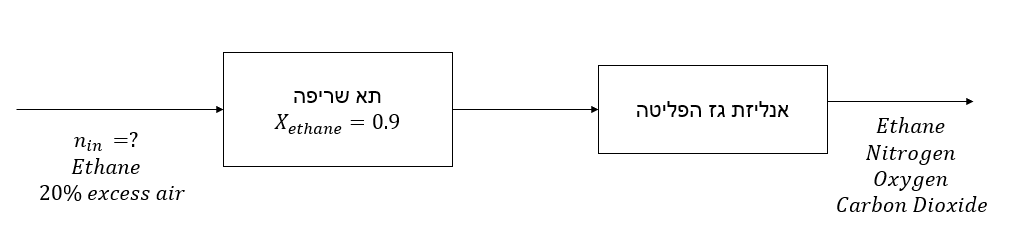
\includegraphics[width=6.5in,height=1.61528in]{images/IntroToCHemEng2/media/image74.png}

מדוע לא רואים מים בתוצרים? מפני שהם מתעבים לפני שמכניסים אותם למכשיר
האנליזה. ציור יותר נכון של המערכת יהיה

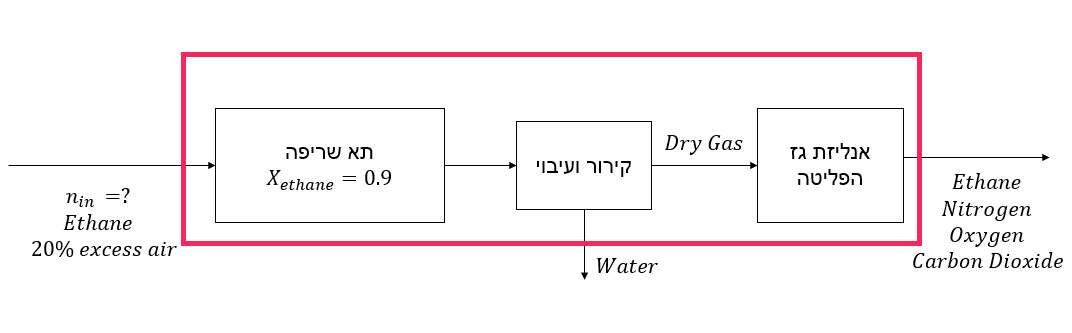
\includegraphics[width=6.5in,height=2.01944in]{images/IntroToCHemEng2/media/image75.png}\\
ניתוח דרגות חופש בסיסי על המערכת המלאה -\\
נעלמים -- בזרם הכניסה --
\(n_{C_{2}H_{6},\ in}\ \ ,\ \ n_{O_{2},\ in}\ \ \ \ ,\ n_{N_{2},in}\)

ביציאה
\(n_{C_{2}H_{6},\ out}\ \ ,\ \ n_{O_{2},\ out}\ \ \ \ ,\ n_{N_{2},out},\ \ \ \ n_{{CO}_{2},\ out}\ \ \ \ ,\ n_{H_{2}O,out}\)

סך הכל 8 נעלמים.

משוואות ואילוצים --

\begin{enumerate}
\def\labelenumi{\arabic{enumi}.}
\item
  בסיס חישוב (100 מול אתאן, לפי השאלה)
\item
  קשר בין חנקן לחמצן באוויר
\item
  קשר בין הדלק שנכנס לאוויר הנכנס (20\% עודף)
\item
  הקשר בין דלק נכנס לדלק יוצא
\item
  מאזני אטומים עצמאיים -- C,H,N,O
\end{enumerate}

סך הכל 8 משוואות.

המשוואה מוגדרת היטב וניתנת לפתרון יחיד.

פתרון

קודם כל ננסח תגובת שריפה עבור אתאן ונאזן

\[C_{2}H_{6} + 3.5\ O_{2} \rightarrow 2CO_{2} + 3H_{2}O\]

נחשב את החמצן התיאורטי לצורך חישוב האוויר שנכנס למערכת.

\[n_{O_{2},\ theroetical} = n_{C_{2}H_{6},\ in}*\frac{\nu_{O_{2}}}{\nu_{C_{2}H_{6}}} = 100mol*3.5 = 350\ mol\ O_{2}\]

אוויר תיאורטי

\[n_{air,theoretical} = \frac{n_{O_{2},\ theroetical}}{0.21} = \frac{350mol}{0.21} = 1670\ mol\ air\]

אוויר עודף

\[n_{fed} = n_{theoretical} \times \left( 1 + \frac{\%\text{Excess}}{100} \right)\]

\[n_{fed} = 1670 \times \left( 1 + \frac{20}{100} \right) = 2000\ mol\ air\]

\[n_{fed,O_{2}} = 420mol\ \ \ \ \ n_{fed,N_{2}} = 1580mol\ \ \ \ \ \]

מה קרה בפועל? נבצע מאזן חומר

אתאן -
\(n_{C_{2}H_{6},\ in} = n_{C_{2}H_{6},\ reacted} + n_{C_{2}H_{6},\ out}\)

\[X = \frac{n_{C_{2}H_{6},\ in} - n_{C_{2}H_{6},\ out}}{n_{C_{2}H_{6},\ in}} = 0.9\]

\[n_{C_{2}H_{6},\ in} = 100mol\ \ ;\ n_{C_{2}H_{6},\ out} = 10mol\ ;\ \ n_{C_{2}H_{6},\ reacted} = 90mol\ \]

חמצן נצרך (לפי המקדמים הסטויכיומטריים)

\[n_{O_{2},\ reacted} = \frac{\nu_{O_{2}}}{\nu_{C_{2}H_{6}}}n_{C_{2}H_{6},\ reacted} = \frac{3.5}{1}*90mol = 315mol\]

מאזן על חמצן

\[n_{O_{2},\ in} = n_{O_{2},\ reacted} + n_{O_{2},\ out}\]

\[n_{O_{2},\ out} = 420mol - 315mol = 105mol\]

פחמן דו חמצני

\[n_{{CO}_{2},gen} = n_{{CO}_{2},\ out}\]

\[n_{{CO}_{2},gen} = \frac{\nu_{{CO}_{2}}}{\nu_{C_{2}H_{6}}}n_{C_{2}H_{6},\ reacted} = \frac{3}{1}*90mol = 270mol\]

מים

\[n_{H_{2}O,gen} = n_{H_{2}O,\ out}\]

\[n_{H_{2}O,gen} = \frac{\nu_{H_{2}O}}{\nu_{C_{2}H_{6}}}n_{C_{2}H_{6},\ reacted} = \frac{2}{1}*90mol = 180mol\]

הרכב על בסיס רטוב

\[\, n_{total,wet}\, = n_{C_{2}H_{6},\ out}\, + \, n_{O_{2},\ out}\, + \, n_{{CO}_{2},\ out}\, + n_{H_{2}O,\ out}\, + \, n_{fed,N_{2}}\, = \, 2145\,\text{ mol}\,\]

\[y_{C_{2}H_{6}} = \frac{10\text{ mol}}{2145\text{ mol}} = 0.47\%\]

\[y_{O_{2}} = \frac{105\text{ mol}}{2145\text{ mol}} = 4.90\%\]

\[y_{CO_{2}} = \frac{180\text{ mol}}{2145\text{ mol}} = 8.39\%\]

\[y_{H_{2}O} = \frac{270\text{ mol}}{2145\text{ mol}} = 12.59\%\]

\[y_{N_{2}} = \frac{1580\text{ mol}}{2145\text{ mol}} = 73.66\%\]

הרכב על בסיס יבש

\[n_{total,wet}\, = n_{C_{2}H_{6},\ out}\, + \, n_{O_{2},\ out}\, + \, n_{{CO}_{2},\ out}\, + \, n_{fed,N_{2}}\, = 1875\text{mol}\]

\[y_{C_{2}H_{6},dry} = \frac{10\text{ mol}}{1875\text{ mol}} = 0.53\%\]

\[y_{O_{2},dry} = \frac{105\text{ mol}}{1875\text{ mol}} = 5.60\%\]

\[y_{CO_{2},dry} = \frac{180\text{ mol}}{1875\text{ mol}} = 9.60\%\]

\[y_{N_{2},dry} = \frac{1580\text{ mol}}{1875\text{ mol}} = 84.27\backslash\%\]

במפעל פטרוכימי גדול פועל כבשן מרכזי המשמש לאספקת חום לתהליכי הייצור. דלק
הכבשן הוא גז מתאן (\(CH_{4}\)) טהור. לאחרונה, הנהלת המפעל החליטה להטמיע
טכנולוגיית "מחזור גזי פליטה" (EGR- Exhaust Gas Recirculation), במטרה
למתן את הטמפרטורות בכבשן ובכך למנוע יצירת תחמוצות חנקן (\(NO_{x}\))
מזהמות. המהנדס הנבחר לתיקון פרוטוקול ההפעלה תוך הקפדה על יציבות התהליך
הוא הסטודנט העצל זרובבל, והוא קיבל לידיו את פרוטוקול ההפעלה המתוכנן.

לפי הפרוטוקול - המתאן מוזן למבער בקצב קבוע של \(100\, mol\text{/}h\).
והמפוחים מכוונים כך שהם יונקים אוויר טרי (יבש) בעודף של 15\%. הגזים
הלוהטים שיוצאים מהכבשן עוברים תחילה דרך יחידת קירור ועיבוי (Condenser).
ביחידה זו, כל אדי המים שנוצרו בשריפה הופכים לנוזל ומסולקים מהמערכת
לטיפול בנפרד. זרם הגז היבש שנותר מפוצל כך ש 40\% מהזרם מוחזר כתחזיר
ומוזרמים יחד עם האוויר הטרי אל הכניסה למבער, ויתר הזרם משתחרר דרך
הארובה. מבדיקות מעבדה עולה כי כל המתאן המוזן למערכת נצרך, אך החמצון אינו
מושלם. הסלקטיביות בין תגובת השריפה המלאה לתגובת השריפה החלקית היא 19.

בבוקר קיבל הסטודנט העצל זרובבל מזכר דחוף מיצרן המבערים. היצרן מתריע כי
המבער תוכנן לעבוד עם תערובת גזים עשירה בחמצן. אם ריכוז החמצן
\(\left( y_{O_{2}} \right)\)בזרם המאוחד הנכנס למבער יורד מתחת ל-18\%,
הלהבה עלולה להפוך ללא יציבה. מצב כזה עלול להוביל לכיבוי פתאומי
("Flame-out") ולסכנת פיצוץ בעת ניסיון הצתה מחדש.

עזרו לסטודנט העצל זרובבל להחליט האם המערכת יציבה. אם לא, מה תמליצו לו
לעשות על מנת לתקן?

\begin{quote}
\textbf{נתאר לעצמינו את השאלה בכמה מילים -}

יש לנו תהליך שריפה של מתאן שנשרף במלואו, רובו (95\%) שריפה מלאה והשאר
שריפה חלקית. המים מעובים ואז גז הפליטה היבש מוחזר כאשר 40\% הולך לתחזיר
ו60\% לזרם סילוק. שואלים אותנו מה אחוז החמצן בנקודת הכניסה של החמצן
לכבשן, והאם זה גדול מ18\%?

כעת נצייר את המערכת כדי להבין את הנתונים. קודם כל נצייר דיאגרמת בלוקים
ונמספר זרמים.

לאחר מכן נוסיף את כל הנתונים שאנחנו מוצאים

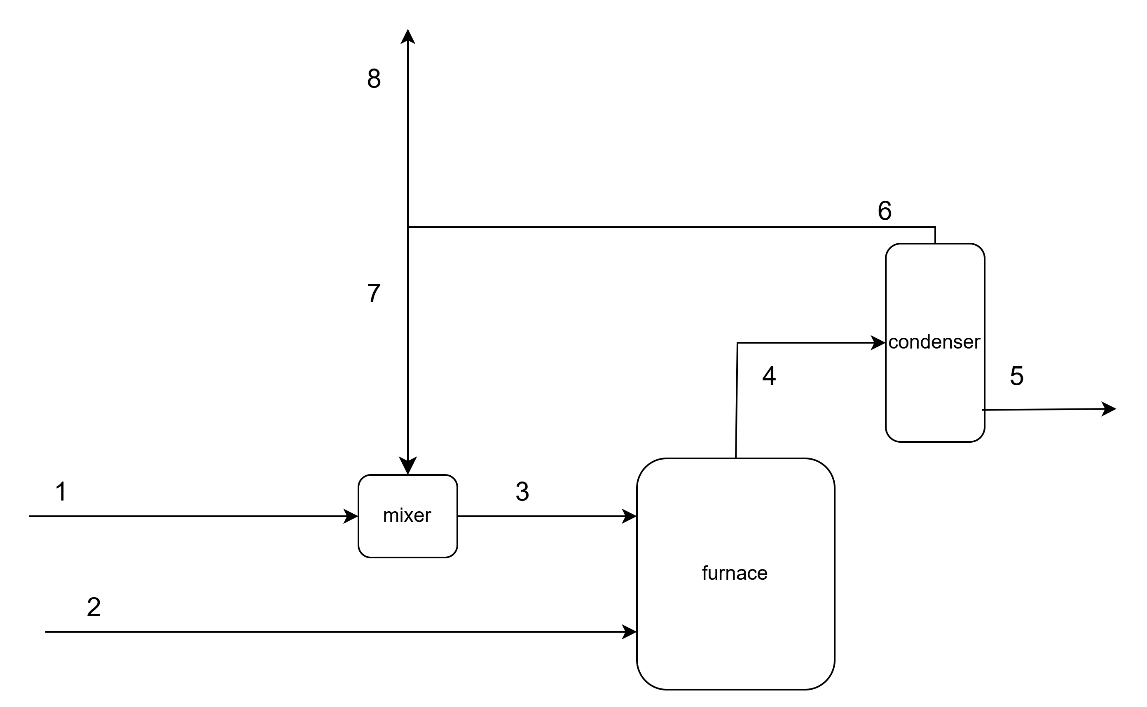
\includegraphics[width=5.18822in,height=3.2004in]{images/IntroToCHemEng2/media/image76.png}
\end{quote}

הנחות -- לשם הנוחות נבחר בסיס חישוב של שעה, ומעכשיו נדבר על ערכים
מוחלטים של מולים

\begin{itemize}
\item
  מצב עמיד
\item
  כל המתאן נשרף
\item
  אין פיח -- רק שריפה מלאה וחלקית
\item
  כל המים מתעבים ויוצאים במעבה.
\item
  זרם כניסה של אויר -- 79\% חנקן והשאר חמצן
\end{itemize}

\begin{quote}
\textbf{ונכניס אליו את כל המידע}

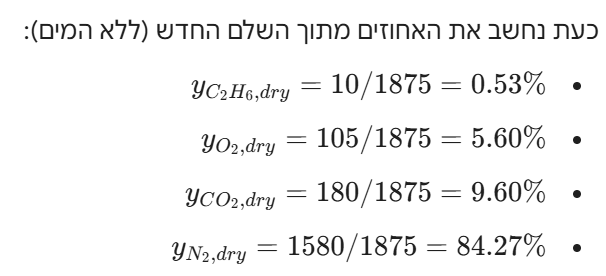
\includegraphics[width=6.7642in,height=2.91329in]{images/IntroToCHemEng2/media/image77.png}
\end{quote}

\textbf{מה שואלים בפועל?} \(y_{3,O_{2}} = ?\), האם הוא גדול מ0.18?

**ניתוח דרגות חופש -- האם זה פתיר?** נסתכל על המערכת המלאה

איזה זרמים חוצים? 1,2,5,8

נעלמים -
\(n_{1},\ n_{5},n_{6},\ y_{6,N_{2}},y_{6,O_{2}},\ y_{6,{CO}_{2}},\xi_{1},\ \xi_{2}\ \)

סך הכל שמונה נעלמים

מה ידוע לנו --

\begin{enumerate}
\def\labelenumi{\arabic{enumi}.}
\item
  שישה מאזנים מולקולריים (מתאן, חמצן, מים, פחמן דו חצמני, פחמן חד חמצני,
  חנקן)
\item
  המרת מתאן 100\%
\item
  סלקטיביות (יחס בין פחמן דו חמצני לפחמן חד חמצני)
\item
  15\% עודף בכניסה
\end{enumerate}

9 משוואות \(DOF = - 1\)

איך זה יכול להיות? נסתכל על זה שוב.\\
\ul{השתמשנו כבר הנתון של המרת המתאן -- בזה שהגדרנו שבזרם 4 אין מתאן ולכן
אסור לספור את זה} בחישובים של דרגות החופש. שישה מאזנים מולקולריים,
סלקטיביות ועודף אויר בכניסה

\[DOF = 8 - 8\]

כלומר, יש לנו מספיק משוואות לסגור את הבעיה ללא הנחות נוספות. בפועל, בגלל
שמדובר בשריפה עם המרה מלאה ויחסי תוצרים נתונים, הזרם היוצא נקבע
חד-משמעית\emph{.}

אבל אין כאן את הערך שמעניין אותנו. לכן נבצע ניתוח דרגות חופש על המיקסר

זרמים -- 1,7,3

נעלמים --
\(n_{1},n_{7},\ y_{6,N_{2}},y_{6,O_{2}},\ y_{6,{CO}_{2}},\ n_{3},\ y_{3,O_{2}},y_{3,N_{2}},y_{3,CO_{2}},\ \)

9 נעלמים

משוואות -- ארבעה מאזנים מולקולריים

\[DOF = 9 - 4 = 5\]

כרגע זה ממש לא פתיר, אבל אם נפתור את המערכת הכוללת

נגלה את \(n_{1},n_{7},\ y_{6,N_{2}},y_{6,O_{2}},\ y_{6,{CO}_{2}},\)

ונשארו לנו רק ארבעת המשתנים של זרם 3
\(n_{3},\ y_{3,O_{2}},y_{3,N_{2}},y_{3,CO_{2}}\) ואז \(DOF = 4 - 4 = 0\)

תכנית לפתרון -

\begin{enumerate}
\def\labelenumi{\arabic{enumi}.}
\item
  נמצא את \(n_{1}\) באמצעות הנתון של אויר עודף
\item
  באמצעות הסלקטיביות ובסיס החישוב נמצא את היקף התגובה של כל אחת מהתגובות
\item
  נחשב שינויים הנובעים מהתגובות עבור כל אחד מהמגיבים/תוצרים
\item
  נחשב מאזנים מולקולריים על כל החומרים
\item
  מאזן על המפצל כדי לראות כמה זורם לכל כיוון
\item
  מאזנים על זרם 3 למצוא את כמות החמצן
\end{enumerate}

\ul{חישוב אויר בכניסה}

כמקובל בהנדסת תהליכים, נגדיר עודף אוויר ביחס לשריפה המלאה הסטויכיומטרית
של מתאן\emph{:}

\[CH_{4} + 2O_{2} \rightarrow CO_{2} + 2H_{2}O\]

כלומר \(2\text{ }mol\text{ }O_{2}\) לכל
\(1\text{ }mol\text{ }CH_{4}\)\emph{.}

לכן, חמצן תיאורטי למתאן (מלא)\emph{:}

\[n_{O_{2},\text{theor}} = 2 \cdot 100 = 200\text{ }kmol\]

עם 15\% עודף אוויר (טרי)\emph{:}

\[n_{O_{2},1} = 1.15 \cdot 200 = 230\text{ }kmol\]

ומכאן ספיקת אוויר טרי\emph{:}

\[n_{air,1} = \frac{n_{O_{2},1}}{y_{O_{2},1}} = \frac{230}{0.21} = 1095.238kmol = 1100\text{ }kmol\]

וחנקן טרי\emph{:}

\[n_{N_{2},2} = n_{air,2}*y_{N_{2},2} = 0.79 \cdot 1100kmol = 865.238\text{ }kmol = 870kmol\]

\ul{מציאת היקף התגובה}

\[\begin{matrix}
CH_{4} + 2O_{2} \rightarrow CO_{2} + 2H_{2}O & \xi_{1} \\
CH_{4} + 1.5O_{2} \rightarrow CO + 2H_{2}O & \xi_{2}
\end{matrix}\]

מתוך מקדם ההמרה והסלקטיביות

\[n_{reacted,CH_{4}} = n_{in,CH_{4}} \cdot X_{CH_{4}}\]

נגדיר את הקפי התגובה

\[n_{reacted,CH_{4}} = \left( \nu_{1,CH_{4}} \cdot \xi_{1} \right) + \left( \nu_{2,CH_{4}} \cdot \xi_{2} \right)\]

והסלקטיביות

\[S = \frac{\nu_{1,CO_{2}} \cdot \xi_{1}}{\nu_{2,CO} \cdot \xi_{2}}\]

כעת נסדר לעצמינו בטבלה את השינוי בכל אחד מהחומרים

\begin{longtable}[]{@{}
  >{\raggedright\arraybackslash}p{(\linewidth - 10\tabcolsep) * \real{0.0935}}
  >{\raggedright\arraybackslash}p{(\linewidth - 10\tabcolsep) * \real{0.1295}}
  >{\raggedright\arraybackslash}p{(\linewidth - 10\tabcolsep) * \real{0.2446}}
  >{\raggedright\arraybackslash}p{(\linewidth - 10\tabcolsep) * \real{0.2446}}
  >{\raggedright\arraybackslash}p{(\linewidth - 10\tabcolsep) * \real{0.1439}}
  >{\raggedright\arraybackslash}p{(\linewidth - 10\tabcolsep) * \real{0.1439}}@{}}
\toprule\noalign{}
\begin{minipage}[b]{\linewidth}\raggedright
רכיב
\end{minipage} & \begin{minipage}[b]{\linewidth}\raggedright
כניסה
\end{minipage} & \begin{minipage}[b]{\linewidth}\raggedright
שינוי מריאקציה 1
\end{minipage} & \begin{minipage}[b]{\linewidth}\raggedright
שינוי מריאקציה 2
\end{minipage} & \begin{minipage}[b]{\linewidth}\raggedright
יציאה
\end{minipage} & \begin{minipage}[b]{\linewidth}\raggedright
הערות
\end{minipage} \\
\midrule\noalign{}
\endhead
\bottomrule\noalign{}
\endlastfoot
\(CH_4\) & \(n_2\) & \(-\nu_{CH_4,1}\,\xi_1\) & \(-\nu_{CH_4,2}\,\xi_2\)
& \(0\) & הכל הגיב (בדיקה) \\
\(O_2\) & \(n_{1,O_2}\) & \(-\nu_{O_2,1}\,\xi_1\) &
\(-\nu_{O_2,2}\,\xi_2\) & \(n_{8,O_2}\) & הנעלם שלנו \\
\(N_2\) & \(n_{1,N_2}\) & \(0\) & \(0\) & \(n_{8,N_2}\) & אינרטי \\
\(CO_2\) & \(0\) & \(\nu_{CO_2,1}\,\xi_1\) & \(0\) & \(n_{8,CO_2}\) &
נוצר רק בריאקציה 1 \\
\(CO\) & \(0\) & \(0\) & \(\nu_{CO,2}\,\xi_2\) & \(n_{8,CO}\) & נוצר רק
בריאקציה 2 \\
\(H_2O\) & \(0\) & \(\nu_{H_2O,1}\,\xi_1\) & \(\nu_{H_2O,2}\,\xi_2\) &
\(n_{5,H_2O}\) & כל המים יוצאים בזרם \\
\end{longtable}

וכעת קל לבנות משוואות עבור כל אחד מהרכיבים

\[0 = n_{2}{- \nu}_{CH_{4},1},\xi_{1}{- \nu}_{CH_{4},2},\xi_{2}\]

\[n_{8,O_{2}} = n_{1,O_{2}}{- \nu}_{O_{2},1},\xi_{1}{- \nu}_{O_{2},2},\xi_{2}\]

\[n_{1,N_{2}} = n_{8,N_{2}}\]

\[n_{8,{CO}_{2}} = \nu_{CO_{2},1},\xi_{1}\]

\[n_{8,CO} = \nu_{CO,2},\xi_{2}\]

\[n_{5,H_{2}O} = \nu_{H_{2}O,1},\xi_{1} + \nu_{H_{2}O,2},\xi_{2}\]

\hfill\break

וכעת יש לנו את כל המשוואות על מנת לפתור את המערכת הגדולה

הצבת המספרים\emph{:}

\[n_{reacted,CH_{4}} = 100\, kmol \cdot 1.0 = 100\, kmol\]

\[n_{reacted,CH_{4}} = 100\ kmol = 1 \cdot \xi_{1} + 1 \cdot \xi_{2}\]

\[S = \frac{\nu_{1,CO_{2}} \cdot \xi_{1}}{\nu_{2,CO} \cdot \xi_{2}}\ \  = > 19 = \frac{1 \cdot \xi_{1}}{1 \cdot \xi_{2}}\]

\[100\ kmol = 19 \cdot \xi_{2} + 1 \cdot \xi_{2} = 20\xi_{2}\]

\[\xi_{2} = 5\ kmol\]

\[\xi_{1} = 95\ kmol\]

ונציב במשוואות ההיקף של החומרים השונים

\[0 = 100 - 1*95\ kmol - 15\ kmol\]

\[n_{8,O_{2}} = 230\text{ }kmol - n_{1,O_{2}}2\xi_{1} - 1.5\xi_{2} = 230\text{ }kmol - n_{1,O_{2}}2*95kmol - 1.5*5kmol = 32\ kmol\]

\[n_{1,N_{2}} = n_{8,N_{2}} = 870kmol\]

\[n_{8,{CO}_{2}} = \nu_{CO_{2},1},\xi_{1} = 1*95\ kmol\]

\[n_{8,CO} = \nu_{CO,2},\xi_{2} = 1*5kmol\]

\[n_{5,H_{2}O} = 2*95\ kmol + 2*5kmol = 200kmol\]

מים במעבה (כל המים מסולקים)\emph{:}

\[{\dot{n}}_{H_{2}O,L} = 200\text{ }kmol/h\] ואנחנו יכולים למצוא את
ההרכב היבש של הזרם היוצא בגז הפליטה

\[n_{8} = n_{8,O_{2}} + n_{8,{CO}_{2}} + n_{8,CO} + n_{8,N_{2}}\]

\[n_{6} = (230kmol - 198kmol) + 95\ kmol + 5kmol + 870kmol = 1002\ kmol = 1000kmol\]

\[y_{6,O_{2}} = \frac{n_{8,O_{2}}}{n_{8}} = \frac{32kmol}{1000kmol} = 3.2\%\]

\[y_{6,{CO}_{2}} = \frac{n_{8,{CO}_{2}}}{n_{8}} = \frac{95kmol}{1000kmol} = 9.5\%\]

\[y_{6,CO} = \frac{n_{8,CO}}{n_{8}} = \frac{5kmol}{1000kmol} = 0.5\%\]

\[y_{6,N_{2}} = \frac{n_{8,N_{2}\ }}{n_{8}} = \frac{870kmol}{1000kmol} = 87\%\]

נזכר מה אנחנו מחפשים -- אחוז החמצן בזרם 3.

לצורך כך נצטרך לעשות מאזנים על המיקסר.

בשביל למצוא את הכניסה למיקסר נשתמש ביחס ההפרדה של המפצל

\[n_{7} = 0.4n_{6} = 0.4*1000kmol = 400kmol\ \ \] מאזן מולים על המיקסר

\[n_{3} = n_{1} + n_{7}\]

\[n_{3} = 1100kmol + 400\ kmol = 1500kmol\]

ונמצא את השבר המולי של החמצן

\[y_{3,O_{2}}\, = \,\frac{n_{1}*y_{1,O_{2}}\, + \, n_{7}*y_{7,O_{2}}}{n_{3,}} = \frac{1100kmol*0.21\, + \, 400kmol*0.032}{1500kmol} = 16.2\%\]

הסף שניתן: 18\% מולרי. מתקבל\emph{:}

\[16.2\% < 18\%\] \textbf{המסקנה הסופית}

ריכוז החמצן בכניסה למבער הוא \emph{16.2\%}. מכיוון שערך זה נמוך מהסף
הנדרש של 18\%, המערכת אינה עומדת בדרישות הבטיחות, והלהבה עלולה
להיכבות\emph{.}\\
המלצה הנדסית (בונוס)\emph{:} כדי לפתור את הבעיה, המפעל יצטרך\emph{:}

\begin{enumerate}
\def\labelenumi{\arabic{enumi}.}
\item
  להקטין את אחוז המחזור (פחות מ-40\%)\emph{.}
\item
  או להגדיל את עודף האוויר בכניסה (יותר מ-15\%)\emph{.}
\end{enumerate}

\subsection{סיכום תגובות
שריפה}\label{ux5e1ux5d9ux5dbux5d5ux5dd-ux5eaux5d2ux5d5ux5d1ux5d5ux5ea-ux5e9ux5e8ux5d9ux5e4ux5d4}

תגובות שריפה הן המקרה הפרטי הנפוץ ביותר של תגובות כימיות בתעשייה. מבחינה
חישובית, חלים עליהן כל חוקי מאזני החומר (המרה, סטויכיומטריה, מגיב
מגביל), אך הן מתאפיינות בז\textquotesingle רגון מקצועי ייחודי\emph{.}

\begin{itemize}
\item
  \textbf{הדלק \emph{(Fuel)}:} לרוב פחמימנים
  \emph{(}\(C_{x}H_{y}\)\emph{).}

  \begin{itemize}
  \tightlist
  \item
    במציאות מכיל אי-ניקיונות: גופרית
    \emph{(}\(S \rightarrow SO_{2}\)\emph{),} אפר (מוצק, יוצא ללא
    שינוי), ומים (מתאדים וצורכים אנרגיה).
  \end{itemize}
\end{itemize}

\begin{itemize}
\item
  \textbf{המחמצן \emph{(Oxidizer)}:} חמצן מולקולרי, לרוב
  מה\textbf{אוויר}

  \begin{itemize}
  \item
    \textbf{הרכב האוויר:} \(21\%\, O_{2},\) \(79\%\, N_{2}\)באחוזים
    מולריים.
  \item
    \textbf{תפקיד החנקן:} אינרטי (נכנס ויוצא ללא שינוי כימי), אך תופס
    נפח, מדלל את החמצן, וסופח חום רב שיוצא בארובה\emph{.}
  \end{itemize}
\item
  \textbf{סוגי שריפה}
\end{itemize}

\begin{itemize}
\item
  \textbf{שריפה מלאה \emph{(Complete)}:} המצב האידיאלי. כל הפחמן הופך
  ל\(CO_{2}\)\emph{,} המימן ל\(H_{2}O\) והגופרית ל\(SO_{2}\)\emph{.}
\item
  \textbf{שריפה חלקית \emph{(Partial)}:} חלק מהפחמן הופך ל-\(CO\) (רעיל
  ובזבזני אנרגטית) או לפיח \emph{(}\(C\)\emph{)}.
\end{itemize}

חישוב כמויות האוויר מתבצע תמיד ביחס לנקודת ייחוס תיאורטית\emph{:}

\begin{longtable}[]{@{}
  >{\centering\arraybackslash}p{(\linewidth - 4\tabcolsep) * \real{0.2059}}
  >{\raggedright\arraybackslash}p{(\linewidth - 4\tabcolsep) * \real{0.2500}}
  >{\raggedright\arraybackslash}p{(\linewidth - 4\tabcolsep) * \real{0.5368}}@{}}
\toprule\noalign{}
\begin{minipage}[b]{\linewidth}\centering
\textbf{המושג}
\end{minipage} & \begin{minipage}[b]{\linewidth}\raggedright
\textbf{הגדרה}
\end{minipage} & \begin{minipage}[b]{\linewidth}\raggedright
\textbf{נוסחה / הערה}
\end{minipage} \\
\midrule\noalign{}
\endhead
\bottomrule\noalign{}
\endlastfoot
\textbf{חמצן תיאורטי}

\emph{(}\(O_{2,theoretical}\)\emph{)} & הכמות הסטויכיומטרית הדרושה
לשריפה \textbf{מלאה} של כל הדלק שהוזן\emph{.} & מחושב לפי משוואת
הריאקציה המלאה בלבד\emph{.} \\
\textbf{אוויר תיאורטי}

\emph{(}\(Air_{theoretical}\)\emph{)} & כמות האוויר המכילה את החמצן
התיאורטי\emph{.} & \(n_{air,th} = \frac{n_{O_{2},th}}{0.21}\) \\
\textbf{אוויר עודף}

\emph{(}\(\%\ Excess\)\emph{)} & מקדם ביטחון תפעולי להבטחת שריפה
מלאה\emph{.} & \(\frac{n_{fed} - n_{th}}{n_{th}} \times 100\%\) \\
\textbf{אוויר מוזן}

\emph{(}\(n_{fed}\)\emph{)} & הכמות שנכנסת פיזית לכבשן\emph{.} &
\(n_{fed} = n_{th}\left( 1 + \frac{\backslash\% Excess}{100} \right)\) \\
\end{longtable}

\textbf{אנליזת גזי פליטה: בסיס רטוב מול יבש}

ההבדל נובע משיטת המדידה (עיבוי מים לפני דגימה)\emph{.}

\begin{itemize}
\tightlist
\item
  בסיס רטוב \emph{(Wet Basis):} ההרכב האמיתי ביציאה מהארובה (כולל אדי
  מים)\emph{.}
\end{itemize}

\[y_{i,wet} = \frac{n_{i}}{n_{total,wet}}\]

\begin{itemize}
\tightlist
\item
  בסיס יבש \emph{(Dry Basis):} ההרכב המדובר לאחר עיבוי וסילוק המים
  (סימולציה של מכשיר מדידה)\emph{.}
\end{itemize}

\[y_{i,dry} = \frac{n_{i}}{n_{total,wet} - n_{H_{2}O}}\]

\begin{itemize}
\tightlist
\item
  במעבר מבסיס יבש (נתון מדידה) לבסיס רטוב (נתון מאזן), חובה להשתמש בנתון
  חיצוני (כגון מאזן אטומי על מימן) כדי לשחזר את כמות המים
  המקורית\emph{.}
\end{itemize}

\section{סיכום מאזני חומר בהנדסת
תהליכים}\label{ux5e1ux5d9ux5dbux5d5ux5dd-ux5deux5d0ux5d6ux5e0ux5d9-ux5d7ux5d5ux5deux5e8-ux5d1ux5d4ux5e0ux5d3ux5e1ux5ea-ux5eaux5d4ux5dcux5d9ux5dbux5d9ux5dd}

מאזן חומר הוא הכלי המרכזי לניתוח תהליכים כימיים ופיזיקליים. הוא מבוסס על
חוק שימור המסה ומאפשר לקשר בין זרמי כניסה, זרמי יציאה, ותהליכים המתרחשים
בתוך מערכת.

הביטוי הכללי של מאזן חומר עבור כל מערכת הוא:

\[
\text{Input} - \text{Output} + \text{Generation} - \text{Consumption} = \text{Accumulation}
\]

ובמצב עמיד:

\[
\text{Input} + \text{Generation} = \text{Output} + \text{Consumption}
\]

השלב הקריטי בכל יישום הוא הגדרת גבול מערכת וזיהוי הזרמים החוצים אותו.

\subsection{מערכות ללא תגובה
כימית}\label{ux5deux5e2ux5e8ux5dbux5d5ux5ea-ux5dcux5dcux5d0-ux5eaux5d2ux5d5ux5d1ux5d4-ux5dbux5d9ux5deux5d9ux5ea}

במערכות פיזיקליות בלבד (ללא תגובה כימית) אין יצירה או צריכה של חומרים:

\begin{itemize}
\tightlist
\item
  לכל מין כימי מתקיים\\
  \(\text{Input} = \text{Output}\)\\
\item
  הפתרון נשען על מאזנים מולקולריים, שברים מולריים ויחסי זרמים.\\
\item
  בדיקת דרגות חופש קובעת האם הנתונים מספיקים לפתרון חד-משמעי.
\end{itemize}

\subsection{מערכות עם תגובה
כימית}\label{ux5deux5e2ux5e8ux5dbux5d5ux5ea-ux5e2ux5dd-ux5eaux5d2ux5d5ux5d1ux5d4-ux5dbux5d9ux5deux5d9ux5ea}

כאשר מתרחשת תגובה כימית:

\begin{itemize}
\tightlist
\item
  מולקולות נוצרות ונצרכות, אך אטומים נשמרים.\\
\item
  קיימות שלוש דרכי ייצוג שקולות של אותה פיזיקה:

  \begin{itemize}
  \tightlist
  \item
    \textbf{מאזן מולקולרי} - כולל איברי יצירה וצריכה לכל מין.
  \item
    \textbf{מאזן אטומי} - סופר אטומים בלבד, ללא תלות בזהות המולקולות.
  \item
    \textbf{מידת ההתקדמות} (\(\xi\)) - מרכזת את השינוי הכימי במשתנה אחד
    לכל ריאקציה.
  \end{itemize}
\item
  כל גישה מייצרת מערכת משוואות שונה, אך הפתרון הפיזיקלי זהה.
\end{itemize}

במערכות עם יותר מריאקציה אחת:

\begin{itemize}
\tightlist
\item
  לא כל משוואת תגובה מוסיפה מידע חדש.
\item
  ריאקציות נספרות רק אם הן \textbf{בלתי תלויות}, כלומר לא ניתנות להרכבה
  כצירוף לינארי של אחרות.
\end{itemize}

\subsection{דרגות חופש
(DOF)}\label{ux5d3ux5e8ux5d2ux5d5ux5ea-ux5d7ux5d5ux5e4ux5e9-dof}

ניתוח דרגות חופש הוא כלי לבדיקת פתירות:

\begin{itemize}
\tightlist
\item
  מספר דרגות החופש של מערכת הוא ההפרש בין מספר הנעלמים למספר המשוואות
  הבלתי תלויות.
\item
  כדי שלמערכת יהיה פתרון יחיד (מערכת מוגדרת היטב), נדרש\\
  \(\mathrm{DOF}=0\).
\item
  במערכות עם תגובה ניתן לבצע את הספירה:

  \begin{itemize}
  \tightlist
  \item
    בגישה האטומית (נעלמים בזרמים בלבד).
  \item
    או בגישת \(\xi\) / מאזן מולקולרי (כולל משתני תגובה).
  \end{itemize}
\item
  אילוצים פיזיקליים ונתונים תפעוליים מצמצמים DOF רק אם הם מערבים את
  נעלמי המערכת.
\end{itemize}

\subsection{תגובות
שריפה}\label{ux5eaux5d2ux5d5ux5d1ux5d5ux5ea-ux5e9ux5e8ux5d9ux5e4ux5d4-1}

תגובות שריפה הן תגובות חשובות בתעשייה:

\begin{itemize}
\tightlist
\item
  דלק (לרוב פחמימנים) מגיב עם חמצן מהאוויר.
\item
  החנקן שבאוויר מתפקד כאינרטי: אינו מגיב אך משפיע על נפח ואנרגיה.
\item
  נעשה שימוש במונחי ייחוס ייעודיים:

  \begin{itemize}
  \tightlist
  \item
    חמצן ואוויר תיאורטיים.
  \item
    אוויר עודף.
  \end{itemize}
\item
  ניתוח גזי פליטה מחייב הבחנה בין בסיס רטוב לבסיס יבש והשלמה באמצעות
  מאזנים אטומיים.
\end{itemize}

\subsection{מערכות עם תחזיר וזרם
סילוק}\label{ux5deux5e2ux5e8ux5dbux5d5ux5ea-ux5e2ux5dd-ux5eaux5d7ux5d6ux5d9ux5e8-ux5d5ux5d6ux5e8ux5dd-ux5e1ux5d9ux5dcux5d5ux5e7}

בתהליכים תעשייתיים המרה מלאה בריאקטור היא חריגה:

\begin{itemize}
\tightlist
\item
  \textbf{תחזיר (Recycle)} מאפשר ניצול חוזר של מגיבים.
\item
  \textbf{זרם סילוק (Purge)} מונע הצטברות אינרטים ותוצרי לוואי.
\item
  קיימת הבחנה מושגית בין:

  \begin{itemize}
  \tightlist
  \item
    המרת מעבר יחיד - מאפיין של הריאקטור.
  \item
    המרה כוללת - מאפיין של המערכת כולה.
  \end{itemize}
\end{itemize}

\subsection{אסטרטגיית
פתרון}\label{ux5d0ux5e1ux5d8ux5e8ux5d8ux5d2ux5d9ux5d9ux5ea-ux5e4ux5eaux5e8ux5d5ux5df}

פתרון בעיות מאזנים הוא תהליך הנדסי:

\begin{itemize}
\tightlist
\item
  בחירת ייצוג (אטומי, מולקולרי, \(\xi\)).
\item
  בחירת גבולות מערכת ותתי-מערכות.
\item
  שימוש בבסיס חישוב מתאים (ולעיתים זמני).
\item
  חתירה לפתרון עקבי פנימית, ולא רק לתוצאה מספרית.
\end{itemize}

מאזן החומר הוא לא רק אוסף משוואות, אלא שפה הנדסית לתיאור תהליכים. שליטה
בכלי זה מאפשרת למהנדסים ולמהנדסות לנתח, לבדוק ולהבין מערכות - מפשוטות
ועד מורכבות - באופן שיטתי, ביקורתי ועקבי.

\bookmarksetup{startatroot}

\chapter{מערכות חד
פאזיות}\label{ux5deux5e2ux5e8ux5dbux5d5ux5ea-ux5d7ux5d3-ux5e4ux5d0ux5d6ux5d9ux5d5ux5ea}

\section{מה נלמד בפרק
הזה?}\label{ux5deux5d4-ux5e0ux5dcux5deux5d3-ux5d1ux5e4ux5e8ux5e7-ux5d4ux5d6ux5d4-3}

\begin{itemize}
\item
  להכיר את המושגים: נוזלים בלתי-דחיסים; חיבור נפחים בנוזלים; משוואת מצב;
  גז אידיאלי; נפח סגולי סטנדרטי; לחץ חלקי; שבר נפחי מול שבר מולרי בגזים
  אידיאליים; גורם דחיסות; משוואות מצב קוביות; טמפרטורה ולחץ קריטיים.
\item
  לחשב צפיפות או נפח של תערובת נוזלים מתוך הרכב נתון, בעזרת נתוני צפיפות
  או הנחת חיבור נפחים; לגזור נוסחת אומדן צפיפות.
\item
  ליישם את משוואת הגז האידיאלי: לחשב את המשתנה החסר, לקבוע את צפיפות
  הגז, ולבחון את תקפות ההנחה בעזרת גורם הדחיסות.
\item
  לפרש ולחשב ספיקות גזים ביחידות סטנדרטיות ובתנאי תהליך אמיתיים.
\item
  לקבוע הרכב תערובת גז אידיאלי מתוך לחצים חלקיים ולחץ כולל.
\item
  לבצע חישובי PVT בעזרת משוואות מצב שונות (ויריאל, ואן-דר-ואלס, SRK,
  compressibility factor).
\item
  לנתח ולפתור מערכות תהליך עם ספיקות נפחיות: לבצע ניתוח דרגות חופש, לנסח
  משוואות, לחשב ולרשום הנחות, ולבחון את סבירותן.
\end{itemize}

\section{מצבי צבירה ודיאגרמת
פאזות}\label{ux5deux5e6ux5d1ux5d9-ux5e6ux5d1ux5d9ux5e8ux5d4-ux5d5ux5d3ux5d9ux5d0ux5d2ux5e8ux5deux5ea-ux5e4ux5d0ux5d6ux5d5ux5ea}

כאשר מהנדס או מהנדסת ניגשים לתכנן או לנתח מערכת תהליכית, נדרש לעיתים
לקבוע תכונות פיזיקליות של חומרי התהליך ולהשתמש בהן כחלק מתיאור המערכת.
תכונות אלו מאפשרות לקשור בין משתנים שונים, ולגזור קשרים הכרחיים לצורך
חישובי מאזן החומר וניתוח הזרמים במערכת.

תכונות פיזיקליות, כגון צפיפות, אינן תמיד ידועות מראש בתנאי העבודה
הרלוונטיים. לשם קביעתן נעזרים במקורות מידע שונים, בהם טבלאות נתונים
ניסיוניים, מאגרי מידע, וקורלציות אמפיריות המתארות את תלות התכונה
בטמפרטורה ולעיתים גם בלחץ. הבחירה בדרך המתאימה לקביעת התכונה, ורמת הדיוק
הנדרשת, הן חלק משיקול הדעת ההנדסי.

\subsection{מצבי
צבירה}\label{ux5deux5e6ux5d1ux5d9-ux5e6ux5d1ux5d9ux5e8ux5d4}

חומרי תהליך יכולים להופיע כמוצקים, נוזלים או גזים, כאשר מצב הצבירה תלוי
בתנאי התהליך, ובראשם הטמפרטורה והלחץ. בניתוח תהליכים, מצב הצבירה קובע
כיצד נבחר לתאר את החומר ואילו תכונות פיזיקליות יהיו רלוונטיות. נוזלים
ומוצקים מתאפיינים בנפח כמעט קבוע ובתלות חלשה בלחץ, ולכן ניתן לרוב לתארם
כחומרים בלתי־דחיסים בקירוב. לעומתם, גזים מתאפיינים בנפח התלוי באופן חזק
בתנאי התהליך, ודורשים טיפול שונה, כפי שנראה בהמשך הפרק.

מעברים בין מצבי צבירה, כגון אידוי, עיבוי או התכה, מתרחשים כאשר תנאי
התהליך משתנים וחוצים גבולות בין אזורי יציבות שונים. גבולות אלו מתוארים
באמצעות דיאגרמות פאזות, המציגות את תחומי הקיום של כל מצב צבירה ואת תנאי
המעבר ביניהם. דיאגרמות אלו משמשות כלי תיאורי חשוב להבנת מצב החומר
בתהליך, אך בקורס זה נשתמש בהן בעיקר לצורך זיהוי תחום העבודה ולא לצורך
ניתוח תרמודינמי מפורט.

סימולציה phase.html

\begin{figure}[H]

{\centering 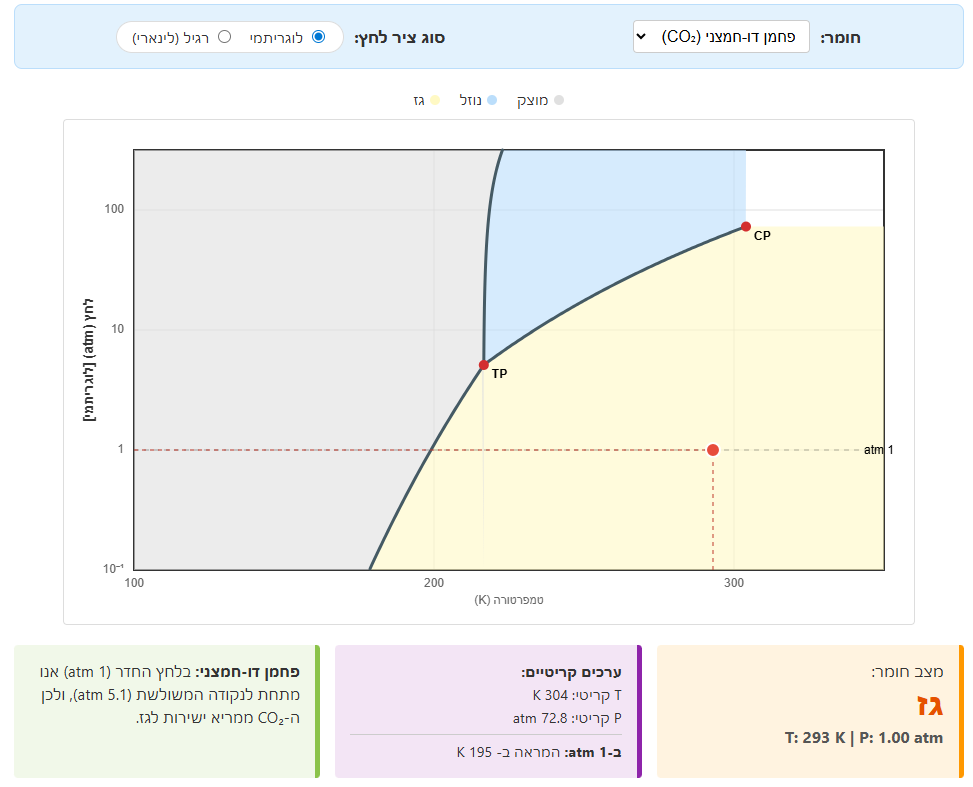
\includegraphics[width=4.70361in,height=3.8046in]{images/IntroToCHemEng2/media/image78.png}

}

\caption{Figure 34 - דיאגרמת פאזות}

\end{figure}%

בניתוח תהליכים נהוג להבחין בין מערכות חד־פאזיות למערכות רב־פאזיות.

פאזה היא אזור במערכת שבו החומר אחיד בתכונותיו הפיזיקליות והכימיות, כגון
הרכב, צפיפות וטמפרטורה.

מערכת חד־פאזית היא מערכת שבה קיים אזור כזה בלבד, כלומר כל החומר נמצא
באותו מצב צבירה ובעל תכונות אחידות.

דוגמאות למערכות חד־פאזיות כוללות נוזל טהור במיכל, תמיסה נוזלית אחידה, או
זרם גז אחיד בצינור. במערכות אלו ניתן לייחס לכל המערכת ערך יחיד של
צפיפות, טמפרטורה והרכב, דבר המאפשר תיאור פשוט יחסית של הזרמים וחישובי
מאזן החומר.

לעומת זאת, במערכת רב־פאזית מתקיימים בו־זמנית אזורים נפרדים בעלי תכונות
שונות, כגון נוזל וגז, או מוצק ונוזל. במערכות כאלה אין אפשרות לתאר את
המערכת כולה באמצעות ערך יחיד של צפיפות או הרכב, ונדרש טיפול נפרד בכל
פאזה. ניתוח מערכות רב־פאזיות מורכב יותר, וידרוש כלים נוספים שלא נעסוק
בהם בשלב זה.

במערכות חד־פאזיות, שבהן ניתן לייחס לחומר תכונות אחידות, ניתן להשתמש
בצפיפות כקשר ישיר בין תיאורים נפחיים לבין כמויות חומר. קשר זה מהווה בסיס
לעבודה עם זרמים של נוזלים ומוצקים בתיאור תהליכים.

עבור כל אחת מהמערכות הבאות, קבעו האם מדובר במערכת \textbf{חד-פאזית} או
\textbf{רב-פאזית}\\
א. כוס מים עם קרח.\\
ב. תרכיז פטל שנמהל במים בצורה מושלמת.\\
ג. בקבוק סודה שנפתח זה עתה (ויוצאות ממנו בועות).

א. \textbf{כוס מים עם קרח: רב-פאזית.} למרות שזהו אותו חומר כימי
(\(\mathbf{H}_{\mathbf{2}}\mathbf{O}\)), יש כאן שני מצבי צבירה שונים
(מוצק ונוזל) עם גבול ברור ביניהם, ותכונות שונות (כמו צפיפות) לכל מצב
צבירה.

ב. \textbf{תרכיז שנמהל: חד-פאזית.} הנוזל אחיד בכל נפחו. אין גבולות
פנימיים המפרידים בין המים לתרכיז (זו תמיסה), ובכל נקודה במערכת התכונות
הפיסיקליות יהיו זהות

ג. \textbf{בקבוק סודה פתוח: רב-פאזית.} יש כאן פאזה נוזלית (המשקה) ופאזה
גזית (בועות הפחמן הדו-חמצני) הנמצאות במגע.

\section{נוזלים ומוצקים: קשר בין מסה, נפח
וצפיפות.}\label{ux5e0ux5d5ux5d6ux5dcux5d9ux5dd-ux5d5ux5deux5d5ux5e6ux5e7ux5d9ux5dd-ux5e7ux5e9ux5e8-ux5d1ux5d9ux5df-ux5deux5e1ux5d4-ux5e0ux5e4ux5d7-ux5d5ux5e6ux5e4ux5d9ux5e4ux5d5ux5ea.}

עד כה, ברוב הדוגמאות והתרגילים בקורס, תיארנו כמויות חומר במונחים של מסה
או מספר מולים. זו בחירה טבעית: מאזן החומר מבוסס על שימור מסה,
וסטוכיומטריה מנוסחת במונחים מולריים. אולם כאשר עוברים מתיאור כימי מופשט
לתיאור של תהליך זורם בפועל, מתברר שאלו אינם המשתנים הנוחים ביותר לעבודה.
במערכות תהליכיות אמיתיות חומר אינו ``נספר'' במולים ואינו ``נשקל'' בכל
רגע, אלא זורם בצינורות, נשאב במשאבות ונמדד לרוב ביחידות של נפח ליחידת
זמן. לכן, כדי לנתח ולפתור מערכות זורמות, עלינו לדעת לקשר בין תיאורים
מבוססי מסה או מולים לבין תיאורים מבוססי נפח.

במערכות תהליכיות רבות, ובפרט כאשר עוסקים בנוזלים, המשתנה הנפחי הוא נקודת
המוצא לחישוב. מיכלים, צינורות, משאבות ומערכות אגירה מתוכננים לפי נפח,
והמידע התפעולי הניתן על תהליך מתייחס לרוב לנפחים או לספיקות נפחיות.
במקרים רבים נוכל לחשב מסה מתוך נפח נתון (או להפך) באמצעות הקשר הפשוט

\[m = \rho V\] כאשר הצפיפות נחשבת קבועה בתנאי התהליך הנתונים. עבור
נוזלים ומוצקים, זוהי לעיתים קרובות הנחה סבירה, שכן נפחם משתנה מעט בלבד
עם לחץ וטמפרטורה בטווחי עבודה תעשייתיים.

עם זאת, בקביעת ערכי צפיפות כחלק מתיאור תהליך, ערכים אלו אינם תמיד זמינים
ישירות, ולעיתים נדרש לאתרם ממקורות חיצוניים. לצורך כך עומדים לרשותנו
סוגים שונים של נתונים פיזיקליים: טבלאות נתונים ניסיוניים, ערכים מדודים
בתנאים סטנדרטיים, וקורלציות אמפיריות המתארות את תלות הצפיפות בטמפרטורה
ולעיתים גם בלחץ.

\subsection{צפיפות של חומרים
טהורים}\label{ux5e6ux5e4ux5d9ux5e4ux5d5ux5ea-ux5e9ux5dc-ux5d7ux5d5ux5deux5e8ux5d9ux5dd-ux5d8ux5d4ux5d5ux5e8ux5d9ux5dd}

צפיפות היא תכונה פיזיקלית אינטנסיבית, המגדירה את היחס בין מסה לנפח של
חומר. עבור חומרים טהורים, הצפיפות נקבעת על ידי זהות החומר ותנאי התהליך,
ובראשם הטמפרטורה והלחץ. במוצקים ובנוזלים, השפעת הטמפרטורה על הצפיפות היא
לרוב משמעותית, בעוד שתלות הצפיפות בלחץ חלשה יחסית וניתנת להזנחה ברוב
טווחי העבודה התעשייתיים.

במערכות תהליכיות, הצפיפות משמשת לקישור בין תיאורים נפחיים של זרמים - כפי
שהם נמדדים ומבוקרים בפועל - לבין כמויות חומר במונחים של מסה או מולים,
הנדרשות לצורך חישובי מאזן חומר. לכן, קביעת ערך צפיפות מתאים אינה שלב
טכני שולי, אלא חלק מרכזי בתיאור המערכת.

\subsubsection{תנאים סטנדרטיים (Standard
Conditions)}\label{ux5eaux5e0ux5d0ux5d9ux5dd-ux5e1ux5d8ux5e0ux5d3ux5e8ux5d8ux5d9ux5d9ux5dd-standard-conditions}

מכיוון שנפח (ולכן גם צפיפות) משתנה כתלות בטמפרטורה ובלחץ, קיים צורך
בבסיס משותף להשוואה ולדיווח נתונים. בסיס זה מכונה "תנאים סטנדרטיים",
והוא משתנה בין ענפי תעשייה ובין ארגונים מדעיים (כגון IUPAC מול תעשיית
הגז והנפט).

בהנדסה כימית ובתהליכים, מקובל להיתקל בשתי הגדרות נפוצות:

\begin{enumerate}
\def\labelenumi{\arabic{enumi}.}
\item
  \textbf{STP (Standard Temperature and Pressure) -} מוגדר לרוב
  כטמפרטורה של \(0^{\circ}C\) (\(273.15\ K\)) ולחץ של \(1\text{ atm}\)
  (או \(1\text{ bar}\) בתקנים חדשים יותר). הגדרה זו נפוצה מאוד בחישובי
  גזים.
\item
  \textbf{SATP (Standard Ambient Temperature and Pressure) -} המכונים
  לעיתים "תנאי חדר", מוגדרים כטמפרטורה של \(25^{\circ}C\)
  (\(298.15\ K\)) ולחץ של \(1\text{ bar}\). נתונים רבים לנוזלים ולמוצקים
  מדווחים סביב טמפרטורה זו.
\end{enumerate}

כאשר אתם שולפים נתון צפיפות מטבלה המציינת "תנאים סטנדרטיים" או מסומנת
בקיצור S.C, בדקו תמיד באותיות הקטנות או במבוא לטבלה מהי הטמפרטורה אליה
מתייחס המקור, שכן ההבדל בין \(0^{\circ}C\) ל-\(25^{\circ}C\) עשוי להיות
משמעותי.

\subsubsection{שימוש בנתונים
טבלאיים}\label{ux5e9ux5d9ux5deux5d5ux5e9-ux5d1ux5e0ux5eaux5d5ux5e0ux5d9ux5dd-ux5d8ux5d1ux5dcux5d0ux5d9ux5d9ux5dd}

הדרך הנפוצה ביותר לקביעת צפיפות של חומר טהור היא שימוש בנתונים ניסיוניים
שפורסמו בספרות המקצועית ובמאגרי נתונים. צפיפויות של חומרים רבים נמדדו
בתנאים מבוקרים, וערכיהן זמינים בטבלאות נתונים ובספרי ייחוס. נתונים אלו
מהווים נקודת מוצא אמינה, וניתן להשתמש בהם ישירות כאשר תנאי המדידה קרובים
לתנאי התהליך הנבחן.

נתונים ניסיוניים לתכונות פיזיקליות של חומרים זמינים במגוון מקורות
ייעודיים. מקורות נפוצים כוללים ספרי ייחוס להנדסת תהליכים, כגון ספרי יד
(handbooks) ומאגרי נתונים מקוונים, המרכזים ערכים שנמדדו בתנאים מבוקרים.
מאגרים אלה מספקים מידע על צפיפות, לחצי אדים, מסיסות ותכונות נוספות,
ולעיתים כוללים גם תלות בטמפרטורה ובלחץ. השימוש במקורות מסוג זה מאפשר
להסתמך על נתונים מבוססים, ולהימנע מהנחות שרירותיות או ממידע שאינו מתועד
כראוי.

נתונים לתכונות פיזיקליות של חומרים, כגון צפיפות, זמינים במאגרי נתונים
ייעודיים ובספרי יד להנדסת תהליכים. מקורות נפוצים כוללים את \emph{CRC
Handbook of Chemistry and Physics}, את \emph{Perry's Chemical Engineers'
Handbook}, ואת מאגר הנתונים המקוון \emph{NIST Chemistry WebBook}. מקורות
אלה מרכזים נתונים ניסיוניים שנמדדו בתנאים מבוקרים, ולעיתים כוללים גם
תלות בטמפרטורה ובלחץ. בעת שימוש בנתונים, חשוב לשים לב לתנאי המדידה
ולוודא התאמה לתנאי התהליך הנבחן. לעיתים ניתן להסתפק בקירוב, ולעיתים נדרש
תיקון או שימוש בנתונים נוספים, בהתאם לרמת הדיוק הנדרשת ולמטרת החישוב.

לגליצרול טהור זמינים הנתונים הבאים:

מקור א:
\(\mathbf{\rho} = \mathbf{1}.\mathbf{26134}\text{ }\mathbf{g}/\mathbf{mL}\)בטמפרטורה
\(\mathbf{20}^{\circ}\mathbf{C}\)

מקור ב:
\(\mathbf{\rho} = \mathbf{1}.\mathbf{23970}\text{ }\mathbf{g}/\mathbf{mL}\)בטמפרטורה
\(\mathbf{60}^{\circ}\mathbf{C}\)

הזרם בתהליך נמצא בטמפרטורה \(\mathbf{25}^{\circ}\mathbf{C}\).\\
באיזה נתון כדאי להשתמש כדי להמיר ספיקה נפחית לספיקה מסתית? נמקו בקצרה.

כדאי להשתמש במקור א' (הנתון ב־\(\mathbf{20}^{\circ}\mathbf{C}\)) משום
שהוא קרוב יותר לתנאי התהליך \(\mathbf{25}^{\circ}\mathbf{C}\). צפיפות של
נוזלים משתנה עם טמפרטורה, ולכן נתון שנמדד קרוב יותר לטמפרטורת העבודה
צפוי להקטין את השגיאה. במקרה הזה, שימוש בנתון
ב־\(\mathbf{60}^{\circ}\mathbf{C}\) עלול להוביל להערכת חסר של הצפיפות
(ומכאן גם של המסה), כי בטמפרטורות גבוהות יותר הצפיפות נמוכה יותר.

כאשר נדרש דיוק גבוה יותר, נעדיף לבצע תיקון טמפרטורה באמצעות קורלציה או
אינטרפולציה בין נתונים.

\subsubsection{שימוש בקורלציות
אמפיריות}\label{ux5e9ux5d9ux5deux5d5ux5e9-ux5d1ux5e7ux5d5ux5e8ux5dcux5e6ux5d9ux5d5ux5ea-ux5d0ux5deux5e4ux5d9ux5e8ux5d9ux5d5ux5ea}

כאשר נדרש ערך צפיפות בטמפרטורה שונה מזו של הנתונים הזמינים, ניתן להיעזר
בקורלציות אמפיריות המתארות את תלות הצפיפות בטמפרטורה. קורלציות אלו הן
ביטויים מתמטיים פשוטים יחסית, אשר הותאמו לנתונים ניסיוניים בטווח מוגדר
של תנאים.

השימוש בקורלציות מאפשר לבצע אינטרפולציה בין נקודות מדידה ידועות, ולעיתים
גם אקסטרפולציה זהירה. עם זאת, יש לזכור כי קורלציות אינן חוקי טבע,
ותקפותן מוגבלת לטווח התנאים שלפיהם פותחו. לכן, בעת שימוש בהן יש לבדוק את
תחום התקפותן ולהעריך את השפעת אי־הוודאות על תוצאות החישוב.

בטקסט נכתב כי "קורלציות אינן חוקי טבע". מהי המשמעות המעשית של משפט זה
עבור מהנדס שצריך לחשב צפיפות בטמפרטורה של
\(\mathbf{8}\mathbf{0}^{\mathbf{\circ}}\mathbf{C}\) כאשר הקורלציה שבידיו
פותחה על סמך נתונים בטווח של
\(\mathbf{1}\mathbf{0}^{\mathbf{\circ}}\mathbf{C - 6}\mathbf{0}^{\mathbf{\circ}}\mathbf{C}\)?
נמקו

\subsubsection{מדידה
ניסיונית}\label{ux5deux5d3ux5d9ux5d3ux5d4-ux5e0ux5d9ux5e1ux5d9ux5d5ux5e0ux5d9ux5ea}

במקרים שבהם לא ניתן למצוא נתונים מתאימים בספרות, או כאשר נדרש דיוק גבוה
במיוחד, הצפיפות נקבעת באמצעות מדידה ניסיונית. בכל מערכת יש גורמים רבים
שמשפיעים ולא תמיד ניתן למדל את כולם, הדרך הכי מדוייקת לדעת את התכונות של
חומר מסויים בתנאים מסויימים היא למדוד אותן. מדידות כאלה מבוצעות באמצעים
ניסיוניים ייעודיים, ונפוצות במיוחד בשלבי פיתוח תהליך, בעבודה עם חומרים
חדשים, או כאשר תנאי התהליך חורגים משמעותית מן התנאים הסטנדרטיים. מדידה
ניסיונית מאפשרת לקבוע את הצפיפות בתנאים המדויקים של המערכת, אך היא כרוכה
בזמן, בעלות ובמאמץ ניסויי. משום כך, היא משמשת בדרך כלל כאשר הדיוק חשוב
ושימוש בנתונים קיימים או בקורלציות אינו מספק מענה מתאים.

\subsubsection{בחירת מקור
הנתונים}\label{ux5d1ux5d7ux5d9ux5e8ux5ea-ux5deux5e7ux5d5ux5e8-ux5d4ux5e0ux5eaux5d5ux5e0ux5d9ux5dd}

הבחירה בין שימוש בנתונים טבלאיים, קורלציות אמפיריות או מדידה ניסיונית
תלויה במטרת החישוב, ברמת הדיוק הנדרשת ובשלב שבו נמצא התהליך ההנדסי.
במקרים רבים, ניתוח ראשוני או חישוב סדר גודל יתבססו על נתונים זמינים
וקירובים פשוטים, בעוד שבשלבים מתקדמים יותר יידרש שימוש בנתונים מדויקים
יותר. היכולת לבחור מקור נתונים מתאים ולהעריך את סבירותו היא חלק בלתי
נפרד מן החשיבה ההנדסית.

בחרו את מקור הנתונים המתאים ביותר בכל מצב (מתוך האפשרויות: טבלה,
קורלציה, מדידה ניסיונית). נמקו

\begin{enumerate}
\def\labelenumi{\arabic{enumi}.}
\item
  תכנון סופי של מערכת תעשייתית, שבה טעות של \(2\%\) בצפיפות תגרום לחריגה
  משמעותית בעמידה במפרט מוצר.
\item
  חישוב ראשוני (סדר גודל) לצורך סקיצה של קטרי צנרת במערכת חדשה.
\item
  נדרש ערך צפיפות בטמפרטורה \(55^{\circ}C\), ויש טבלה רק
  ב-\(20^{\circ}C\), אך קיימת קורלציה התקפה עד \(80^{\circ}C\).
\end{enumerate}

\textbf{1. מדידה ניסיונית} (או נתונים ניסיוניים מאוד ספציפיים לתנאי
התהליך, אם קיימים) - כי דרוש דיוק גבוה והשפעת השגיאה קריטית.

\textbf{2. טבלה} (או ערך סטנדרטי אמין) - כי המטרה היא סדר גודל ולא נדרש
דיוק גבוה.

\textbf{3. קורלציה} - כי היא מאפשרת התאמה לטמפרטורה הרצויה בתוך תחום
התקפות, בעוד שטבלה ב-\(20^{\circ}C\) אינה מתאימה ישירות.

\subsection{צפיפות של תערובות חד
פאזיות}\label{ux5e6ux5e4ux5d9ux5e4ux5d5ux5ea-ux5e9ux5dc-ux5eaux5e2ux5e8ux5d5ux5d1ux5d5ux5ea-ux5d7ux5d3-ux5e4ux5d0ux5d6ux5d9ux5d5ux5ea}

עד כה עסקנו בקביעת צפיפות של חומרים טהורים במערכות חד־פאזיות, שבהן ניתן
לייחס לחומר ערך צפיפות יחיד בתנאי תהליך נתונים. כאשר החומר במערכת הוא
תערובת של נוזלים, מתווסף משתנה חדש - ההרכב - ולכן הצפיפות אינה תכונה
``נתונה מראש'' אלא תוצאה של שילוב הרכיבים. במצב כזה נדרש לקשר בין הרכב
התערובת לבין הנפח הכולל שלה, כדי שנוכל להמשיך ולהמיר בין תיאורים נפחיים
לבין מסה או מולים לצורך חישובי מאזן חומר.

כאשר עוסקים בחומר טהור, הקשר בין מסה לנפח נקבע באמצעות ערך צפיפות יחיד.
אולם כאשר החומר במערכת הוא תערובת של נוזלים, מתעוררת שאלה עקרונית: כיצד
נקבע נפח התערובת מתוך נפחי הרכיבים המרכיבים אותה?

באופן אינטואיטיבי, ניתן לחשוב שנפח תערובת של שני נוזלים שווה לסכום
נפחיהם לפני הערבוב. כלומר, אם מערבבים נפח נתון של נוזל אחד עם נפח נתון
של נוזל אחר, ניתן לצפות שהנפח הכולל יהיה פשוט סכום שני הנפחים.
אינטואיציה זו נפוצה, והיא משמשת לעיתים כהנחת עבודה סמויה. עם זאת, מבחינה
פיזיקלית אין הכרח שנפחי הרכיבים יתחברו בצורה פשוטה. ערבוב נוזלים עשוי
לגרום לשינוי בסידור המולקולרי, ולפיכך גם לשינוי בנפח הכולל. לכן, אף על
פי שבפועל נהוג לעיתים להשתמש בחיבור נפחים באופן ישיר כחלק מחישוב תהליכי,
אין לראות בכך צעד אוטומטי. חיבור נפחים הוא הנחת עבודה שיש להכיר בה
במפורש, ולהבין באילו מצבים היא סבירה ובאילו מקרים היא עלולה להוביל
לשגיאה.

\subsubsection{אדטיביות של
נפחים}\label{ux5d0ux5d3ux5d8ux5d9ux5d1ux5d9ux5d5ux5ea-ux5e9ux5dc-ux5e0ux5e4ux5d7ux5d9ux5dd}

\textbf{הנחת חיבור נפחים (אדטיביות של נפחים)} נפח התערובת שווה לסכום
נפחי הרכיבים המרכיבים אותה לפני הערבוב. כלומר, אם תערובת מורכבת ממספר
רכיבים, כל אחד בנפח נתון, אזי הנפח הכולל של התערובת מתקבל מחיבור נפחי
הרכיבים.

הנחה זו מאפשרת לקשר בין הרכב התערובת לבין נפחה בצורה ישירה, ולכן גם לחשב
צפיפות תערובת מתוך צפיפויות הרכיבים. במונחים חישוביים, היא מפשטת את
הבעיה באופן משמעותי, ומאפשרת להמשיך לעבוד עם תיאורים נפחיים כחלק מניתוח
תהליכים זורמים. עם זאת, חשוב להדגיש כי מדובר \textbf{בהנחה ולא בחוק
פיזיקלי} .חיבור נפחים אינו מובטח מבחינה עקרונית, והוא משקף קירוב שבו
מניחים כי ערבוב הרכיבים אינו גורם לשינוי נפח כולל. הנחה זו סבירה בעיקר
כאשר מדובר בנוזלים בעלי מבנה מולקולרי דומה, או כאשר השפעת האינטראקציות
בין הרכיבים על הנפח הכולל קטנה ביחס לדיוק הנדרש בחישוב.

\subsubsection{חישוב צפיפות של
תערובת}\label{ux5d7ux5d9ux5e9ux5d5ux5d1-ux5e6ux5e4ux5d9ux5e4ux5d5ux5ea-ux5e9ux5dc-ux5eaux5e2ux5e8ux5d5ux5d1ux5ea}

בהנחת חיבור נפחים, ניתן לחשב את צפיפותה של תערובת נוזלים בשתי דרכים
שונות, בהתאם לאופן שבו הרכב התערובת נתון. אף ששתי הדרכים נשענות על אותה
הנחת עבודה, הן מבוססות על תיאורי הרכב שונים - שברי מסה לעומת שברי נפח -
ולכן אינן בהכרח מניבות את אותה תוצאה. ההבדל בין התוצאות נובע מכך שהמעבר
בין תיאורי ההרכב אינו טריוויאלי ותלוי בצפיפויות הרכיבים.

\ul{חישוב צפיפות תערובת מתוך שברי נפח}

כעת נבחן תערובת של שני נוזלים, A ו־B, כאשר הרכב התערובת נתון באמצעות
שברי נפח \(\phi_{A}\), \(\phi_{B}\). בהנחת חיבור נפחים, הנפח הכולל הוא
סכום נפחי הרכיבים, והמסה של כל רכיב מתקבלת כמכפלת נפחו בצפיפותו. צפיפות
התערובת מתקבלת לכן כ־

\[\rho_{\text{mix}} = \phi_{A}\rho_{A} + \phi_{B}\rho_{B}\]

כאשר יש לנו את השברים הנפחיים, צפיפות תערובת עבור תערובת עם n רכיבים
תהיה

\[\rho_{\text{mix}} = \sum_{i = 1}^{n}\phi_{i}\rho_{i}\] כאשר \(i\) הוא
הרכיב, \(\rho_{i}\) זו צפיפות הרכיב ו-\(\phi_{i}\) הוא השבר הנפחי של
הרכיב בתמיסה.

\ul{חישוב צפיפות תערובת מתוך שברי מסה}

נבחן תחילה תערובת חד־פאזית של שני נוזלים, A ו-B. נסמן את המסות של
הרכיבים ב־\(m_{A}\), \(m_{B}\), ואת צפיפויותיהם ב־\(\rho_{A}\),
\(\rho_{B}\). צפיפות התערובת מוגדרת כיחס בין המסה הכוללת לבין הנפח
הכולל:

\[\rho_{\text{mix}} = \frac{m_{A} + m_{B}}{V_{A} + V_{B}}\] בהנחת חיבור
נפחים, נפח כל רכיב בנפרד מתקבל מחלוקת המסה שלו בצפיפות המתאימה:

\[V_{A} = \frac{m_{A}}{\rho_{A}},V_{B} = \frac{m_{B}}{\rho_{B}}\]

הצבה בביטוי לצפיפות התערובת נותנת:

\[\rho_{\text{mix}} = \frac{m_{A} + m_{B}}{\frac{m_{A}}{\rho_{A}} + \frac{m_{B}}{\rho_{B}}}\]
נגדיר את השברים המסתיים

\[x_{A} = \frac{m_{A}}{m_{A} + m_{B}},x_{B} = \frac{m_{B}}{m_{A} + m_{B}}\]
נקבל:

\[\rho_{\text{mix}} = \frac{1}{\frac{x_{A}}{\rho_{A}} + \frac{x_{B}}{\rho_{B}}}\]

הצפיפות של תערובת הכוללת \(n\) רכיבים שהרכבה נתון על ידי שברים מסתיים

\[\rho_{\text{mix}} = \frac{1}{\sum_{i = 1}^{n}\frac{x_{i}}{\rho_{i}}}\]
כאשר \(i\) הוא הרכיב, \(\rho_{i}\) זו צפיפות הרכיב ו-\(x_{i}\) הוא השבר
המסתי של הרכיב בתמיסה.

שתי הדרכים לחישוב צפיפות של תערובת נוזלים נשענות על אותה הנחת עבודה -
חיבור נפחים - אך הן מתאימות למצבים שונים. כאשר הרכב התערובת נתון בשברי
נפח, החישוב ישיר ואינטואיטיבי, ומתבסס על סכימה משוקללת של צפיפויות
הרכיבים. לעומת זאת, כאשר הרכב התערובת נתון בשברי מסה, יש לחשב תחילה את
תרומת כל רכיב לנפח הכולל, ולכן מתקבל ביטוי שונה לצפיפות התערובת. חשוב
לבחור בדרך החישוב בהתאם לאופן שבו הרכב התערובת נתון, ולא לנסות לערבב בין
שתי הגישות. שברי מסה ושברי נפח מתארים תערובות שונות מבחינה פיזיקלית,
והחלפה ביניהם ללא חישוב מפורש עלולה להוביל לתוצאה שגויה.

תערובת נוזלים מורכבת משני רכיבים, A ו-B. צפיפויות הרכיבים הן:

\[\rho_{A} = 800\text{ }kg/m^{3},\rho_{B} = 1200\text{ }kg/m^{3}\]

א. חשבו את צפיפות התערובת בהנחת חיבור נפחים, כאשר שברי \ul{המסה} הם
\(x_{A} = 0.5\), \(x_{B} = 0.5\).\\
ב. חשבו את צפיפות התערובת בהנחת חיבור נפחים, כאשר שברי \ul{הנפח} הם
\(\phi_{A} = 0.5\), \(\phi_{B} = 0.5\).\\
ג. השוו בין התוצאות והסבירו בקצרה את מקור ההבדל.

א. לפי שברי מסה:

\[\rho_{\text{mix}} = \frac{1}{\frac{0.5}{800} + \frac{0.5}{1200}} \approx 960\text{ }kg/m^{3}\]

ב. לפי שברי נפח:

\[\rho_{\text{mix}} = 0.5 \cdot 800 + 0.5 \cdot 1200 = 1000\text{ }kg/m^{3}\]

ג. התקבלו ערכים שונים משום ששברי מסה ושברי נפח מתארים תערובות שונות
מבחינה פיזיקלית. המעבר בין התיאורים תלוי בצפיפויות הרכיבים, ולכן גם תחת
אותה הנחת חיבור נפחים מתקבלות תוצאות שונות.

\subsection{סיכום -- צפיפויות של נוזלים
וגזים}\label{ux5e1ux5d9ux5dbux5d5ux5dd-ux5e6ux5e4ux5d9ux5e4ux5d5ux5d9ux5d5ux5ea-ux5e9ux5dc-ux5e0ux5d5ux5d6ux5dcux5d9ux5dd-ux5d5ux5d2ux5d6ux5d9ux5dd}

\begin{itemize}
\item
  נוזלים ומוצקים במערכות חד־פאזיות מתאפיינים בנפח כמעט קבוע בתנאי תהליך
  נתונים.
\item
  הצפיפות היא תכונה פיזיקלית אינטנסיבית, המשמשת לקישור בין נפח לבין כמות
  חומר (מסה או מולים).
\item
  צפיפות של חומר טהור נקבעת מתוך נתונים ניסיוניים, קורלציות אמפיריות, או
  מדידה ניסיונית, בהתאם לרמת הדיוק הנדרשת.
\item
  בתערובות נוזלים, הצפיפות תלויה גם בהרכב התערובת ולא רק בזהות הרכיבים.
\item
  חישוב צפיפות של תערובת נוזלים מבוסס לרוב על הנחת חיבור נפחים.
\item
  שברי נפח ושברי מסה אינם שקולים, והחלפה ביניהם ללא חישוב מפורש עלולה
  להוביל לשגיאה
\end{itemize}

\section{גזים: כשהנפח תלוי בתנאי
התהליך}\label{ux5d2ux5d6ux5d9ux5dd-ux5dbux5e9ux5d4ux5e0ux5e4ux5d7-ux5eaux5dcux5d5ux5d9-ux5d1ux5eaux5e0ux5d0ux5d9-ux5d4ux5eaux5d4ux5dcux5d9ux5da}

צפיפות מוגדרת כיחס בין מסה לנפח. עבור כמות נתונה של חומר, המסה קבועה,
ולכן כל שינוי בצפיפות נובע משינוי בנפח. בנוזלים ובמוצקים, שינויי נפח
כתוצאה משינויים בלחץ ובטמפרטורה הם קטנים יחסית בטווחי עבודה תעשייתיים,
ולכן הצפיפות ניתנת לרוב להתייחסות כקבועה בקירוב. בגזים, לעומת זאת, גם
שינוי מתון יחסית בלחץ או בטמפרטורה עלול להוביל לשינוי משמעותי בנפח,
ובהתאם גם בצפיפות. מסיבה זו, בגזים אין משמעות לצפיפות ללא ציון מפורש של
תנאי התהליך.

אותו גז, באותה כמות חומר, יכול לתפוס נפחים שונים מאוד בלחצים ובטמפרטורות
שונות. כתוצאה מכך, הצפיפות של גז אינה תכונה קבועה של החומר בלבד, אלא
תלויה באופן ישיר בלחץ ובטמפרטורה שבהם הוא נמצא. כדי לקבוע צפיפות של גז,
אין די בידיעת זהות החומר או כמותו - יש צורך גם בקשר המתאר כיצד הנפח
משתנה כתלות בתנאי התהליך. משמעות הדבר בהנדסת תהליכים היא שנפח אינו יכול
לשמש כמשתנה ``שקט'' כפי שהיה בנוזלים. כדי לקשר בין תיאורים נפחיים לבין
כמויות חומר בגזים, נדרש מודל הקושר בין נפח, טמפרטורה, לחץ וכמות חומר.
קשרים כאלה מכונים \textbf{משוואות מצב}, משום שהם מתארים את מצב הגז בתנאי
תהליך נתונים, ללא תלות במסלול שבו הגיע למצב זה.

\subsection{משוואת הגז
האידיאלי}\label{ux5deux5e9ux5d5ux5d5ux5d0ux5ea-ux5d4ux5d2ux5d6-ux5d4ux5d0ux5d9ux5d3ux5d9ux5d0ux5dcux5d9}

הקשר הפשוט והנפוץ ביותר לתיאור התנהגות של גזים הוא \textbf{משוואת הגז
האידיאלי}.

משוואת הגז האידיאלי קושרת בין לחץ, נפח, טמפרטורה וכמות חומר, ומאפשרת
לחשב כל אחד מן הגדלים הללו כאשר האחרים ידועים:

\[PV = nRT\]

כאשר \(P\) הוא הלחץ, \(V\) הוא הנפח, \(n\)הוא מספר המולים, \(T\)היא
הטמפרטורה המוחלטת, ו-\(R\) הוא קבוע הגזים האוניברסלי. משוואה זו מתארת את
מצב הגז בתנאי תהליך נתונים, והיא אינה תלויה בזהות החומר אלא רק בכמותו
ובתנאים שבהם הוא נמצא.

משוואת הגז האידיאלי קושרת בין ארבעה גדלים: לחץ, נפח, טמפרטורה וכמות
חומר. משמעות הקשר היא שלמצב הגז אין משתנה אחד ``חופשי'': שינוי באחד מן
הגדלים מחייב שינוי באחרים. עבור כמות חומר נתונה -- אם נקבע את הלחץ
והטמפ\textquotesingle{} אנחנו למעשה מגדירים את הנפח שהגז תופס. אם נשנה
את הנפח אחד (או שני) המשתנים האחרים חייבים להשתנות על מנת לאזן את
השינוי.

המונח גז אידיאלי אינו מתאר גז שקיים בפועל, אלא מודל תיאורי פשוט להתנהגות
של גזים. במודל זה מתקבלות שתי הנחות מרכזיות: נפח המולקולות המרכיבות את
הגז זניח ביחס לנפח הכולל, ואין ביניהן אינטראקציות משמעותיות פרט
להתנגשויות רגעיות. הנחות אלו מאפשרות לנסח קשר מתמטי פשוט בין תנאי התהליך
לבין כמות החומר. המונח ``אידיאלי'' משקף את העובדה שהמודל אינו מתאר
במלואו את ההתנהגות הפיזיקלית של גזים אמיתיים. עם זאת, ברוב היישומים
ההנדסיים השגרתיים, שבהם הגזים פועלים בלחצים שאינם גבוהים במיוחד
ובטמפרטורות הרחוקות מתנאי עיבוי, ההתנהגות בפועל קרובה מאוד להתנהגות
אידיאלית.

משום כך, משוואת הגז האידיאלי משמשת כמודל עבודה ראשון בניתוח תהליכים
הכוללים גזים. היא מאפשרת לבצע חישובים נפחיים, לקשר בין מדידות תפעוליות
לבין כמויות חומר, ולבנות הבנה תהליכית ברורה לפני שמוסיפים מורכבות. בהמשך
נראה כיצד ומתי יש לבחון את תקפות ההנחה האידיאלית, ומה עושים כאשר היא
אינה מספקת.

תרגיל -- התנהגות של גז אידיאלי

ענו על השאלות הבאות באמצעות הסימולציה

https://phet.colorado.edu/sims/html/gas-properties/latest/gas-properties\_all.html

\begin{enumerate}
\def\labelenumi{\arabic{enumi}.}
\tightlist
\item
  קבעו מספר חלקיקים קבוע וטמפרטורה קבועה. מה קורה ללחץ כאשר משנים את נפח
  הכלי באמצעות הבוכנה? נסו להסביר את התוצאה במונחים של תנועת חלקיקים
  והתנגשויות בדפנות.\\
\item
  כעת השאירו את הנפח קבוע והעלו את הטמפרטורה. מה קורה ללחץ? מה השתנה
  בתנועת החלקיקים ברמה המיקרוסקופית?\\
\item
  החזירו את הטמפרטורה לערך המקורי, הגדירו טמפרטורה קבועה, והוסיפו
  חלקיקים למערכת. כיצד משתנה הלחץ כאשר הנפח קבוע? האם התוצאה תלויה בזהות
  החלקיקים או רק במספרם?\\
\item
  נסו לשנות שני משתנים בו־זמנית (למשל: הקטנת נפח והורדת טמפרטורה). האם
  ניתן לצפות מראש את כיוון השינוי בלחץ? מה מקשה על ניבוי אינטואיטיבי
  במצב כזה?
\end{enumerate}

מה יקרה ולמה?

נמקו באופן איכותי (ללא שימוש במספרים) במונחים של לחץ, נפח, טמפרטורה או
צפיפות.

א. שקית חטיפים במטוס

שקית חטיפים סגורה נארזה בגובה פני הים. במהלך הטיסה, כאשר המטוס מגיע
לגובה שיוט, השקית מתנפחת. מה השתנה בתנאי הסביבה שגרם לכך? כיצד השינוי
משפיע על נפח הגז שבתוך השקית?

ב. כדור פורח

כדור פורח עומד על הקרקע ומחומם באמצעות מבער. בזמן החימום הכדור מתחיל
להתרומם, אף על פי שהאוויר שבתוכו זהה בהרכבו לאוויר שמסביב. איזה משתנה
תהליכי משתנה בתוך הכדור? כיצד שינוי זה מוביל להתרוממות?

ג. צמיג רכב ביום חם

לחץ האוויר בצמיג נמדד בבוקר קר. לאחר נסיעה ארוכה ביום חם, הלחץ בצמיג
גבוה יותר. מה גרם לשינוי בלחץ? מדוע נפח הצמיג כמעט ואינו משתנה למרות
זאת?

פתרון

א. שקית חטיפים במטוס

השקית נאטמה בגובה פני הים, ולכן כמות הגז שבתוכה קבועה. במהלך העלייה
לגובה, לחץ האוויר החיצוני קטן משמעותית. כך שהלחץ בתוך השקית גדול מהלחץ
מחוץ לשקית. הגז בתוך השקית מתרחב עד שלחצו משתווה ללחץ הסביבה, ולכן נפח
השקית גדל והיא מתנפחת.\\
זהו תהליך שבו הלחץ החיצוני משתנה, והנפח של הגז מתאים את עצמו לשינוי.

ב. כדור פורח

האוויר בתוך הכדור מחומם, בעוד שהכדור פתוח בתחתיתו ולכן הלחץ בתוכו נשאר
קרוב ללחץ האטמוספרי. חימום האוויר מגדיל את נפח האוויר עבור אותה כמות
חומר, ולכן צפיפות האוויר בתוך הכדור קטנה. כאשר הצפיפות הממוצעת בתוך
הכדור נמוכה מצפיפות האוויר החיצוני, מתקבל כוח עילוי כלפי מעלה.\\
זהו תהליך שבו הלחץ כמעט קבוע, והשינוי בטמפרטורה מתבטא בשינוי צפיפות.

ג. צמיג רכב ביום חם

במהלך הנסיעה האוויר בצמיג מתחמם עקב חיכוך והעברת חום מהכביש. נפח הצמיג
כמעט קבוע, וכמות הגז שבתוכו אינה משתנה. לכן העלייה בטמפרטורה מתבטאת
בעלייה בלחץ האוויר בתוך הצמיג.\\
זהו תהליך שבו הנפח כמעט קבוע, והשינוי בטמפרטורה גורם לשינוי בלחץ.

\subsubsection{\texorpdfstring{קבוע הגזים האידיאליים (R) אם נבודד את R
מתוך משוואת הגז האידיאלי, נקבל את הביטוי הבא - \(R = \frac{PV}{nT}\)
משמעות הדבר היא שעבור כל גז אידיאלי בעולם, בכל מצב נתון, היחס בין מכפלת
הלחץ והנפח לבין כמות החומר והטמפרטורה הוא \textbf{ערך קבוע ובלתי משתנה}.
הערך של R משמש למעשה כ"מתרגם" בין שפת הלחץ והנפח שבחרנו לבין שפת האנרגיה
והטמפרטורה ולכן הוא תלוי ביחידות בהן אנחנו משתמשים. להלן הערכים הנפוצים
ביותר, מסודרים לפי מערכת היחידות של הלחץ
והנפח:}{קבוע הגזים האידיאליים (R) אם נבודד את R מתוך משוואת הגז האידיאלי, נקבל את הביטוי הבא - R = \textbackslash frac\{PV\}\{nT\} משמעות הדבר היא שעבור כל גז אידיאלי בעולם, בכל מצב נתון, היחס בין מכפלת הלחץ והנפח לבין כמות החומר והטמפרטורה הוא ערך קבוע ובלתי משתנה. הערך של R משמש למעשה כ"מתרגם" בין שפת הלחץ והנפח שבחרנו לבין שפת האנרגיה והטמפרטורה ולכן הוא תלוי ביחידות בהן אנחנו משתמשים. להלן הערכים הנפוצים ביותר, מסודרים לפי מערכת היחידות של הלחץ והנפח:}}\label{ux5e7ux5d1ux5d5ux5e2-ux5d4ux5d2ux5d6ux5d9ux5dd-ux5d4ux5d0ux5d9ux5d3ux5d9ux5d0ux5dcux5d9ux5d9ux5dd-r-ux5d0ux5dd-ux5e0ux5d1ux5d5ux5d3ux5d3-ux5d0ux5ea-r-ux5deux5eaux5d5ux5da-ux5deux5e9ux5d5ux5d5ux5d0ux5ea-ux5d4ux5d2ux5d6-ux5d4ux5d0ux5d9ux5d3ux5d9ux5d0ux5dcux5d9-ux5e0ux5e7ux5d1ux5dc-ux5d0ux5ea-ux5d4ux5d1ux5d9ux5d8ux5d5ux5d9-ux5d4ux5d1ux5d0---r-fracpvnt-ux5deux5e9ux5deux5e2ux5d5ux5ea-ux5d4ux5d3ux5d1ux5e8-ux5d4ux5d9ux5d0-ux5e9ux5e2ux5d1ux5d5ux5e8-ux5dbux5dc-ux5d2ux5d6-ux5d0ux5d9ux5d3ux5d9ux5d0ux5dcux5d9-ux5d1ux5e2ux5d5ux5dcux5dd-ux5d1ux5dbux5dc-ux5deux5e6ux5d1-ux5e0ux5eaux5d5ux5df-ux5d4ux5d9ux5d7ux5e1-ux5d1ux5d9ux5df-ux5deux5dbux5e4ux5dcux5ea-ux5d4ux5dcux5d7ux5e5-ux5d5ux5d4ux5e0ux5e4ux5d7-ux5dcux5d1ux5d9ux5df-ux5dbux5deux5d5ux5ea-ux5d4ux5d7ux5d5ux5deux5e8-ux5d5ux5d4ux5d8ux5deux5e4ux5e8ux5d8ux5d5ux5e8ux5d4-ux5d4ux5d5ux5d0-ux5e2ux5e8ux5da-ux5e7ux5d1ux5d5ux5e2-ux5d5ux5d1ux5dcux5eaux5d9-ux5deux5e9ux5eaux5e0ux5d4.-ux5d4ux5e2ux5e8ux5da-ux5e9ux5dc-r-ux5deux5e9ux5deux5e9-ux5dcux5deux5e2ux5e9ux5d4-ux5dbux5deux5eaux5e8ux5d2ux5dd-ux5d1ux5d9ux5df-ux5e9ux5e4ux5ea-ux5d4ux5dcux5d7ux5e5-ux5d5ux5d4ux5e0ux5e4ux5d7-ux5e9ux5d1ux5d7ux5e8ux5e0ux5d5-ux5dcux5d1ux5d9ux5df-ux5e9ux5e4ux5ea-ux5d4ux5d0ux5e0ux5e8ux5d2ux5d9ux5d4-ux5d5ux5d4ux5d8ux5deux5e4ux5e8ux5d8ux5d5ux5e8ux5d4-ux5d5ux5dcux5dbux5df-ux5d4ux5d5ux5d0-ux5eaux5dcux5d5ux5d9-ux5d1ux5d9ux5d7ux5d9ux5d3ux5d5ux5ea-ux5d1ux5d4ux5df-ux5d0ux5e0ux5d7ux5e0ux5d5-ux5deux5e9ux5eaux5deux5e9ux5d9ux5dd.-ux5dcux5d4ux5dcux5df-ux5d4ux5e2ux5e8ux5dbux5d9ux5dd-ux5d4ux5e0ux5e4ux5d5ux5e6ux5d9ux5dd-ux5d1ux5d9ux5d5ux5eaux5e8-ux5deux5e1ux5d5ux5d3ux5e8ux5d9ux5dd-ux5dcux5e4ux5d9-ux5deux5e2ux5e8ux5dbux5ea-ux5d4ux5d9ux5d7ux5d9ux5d3ux5d5ux5ea-ux5e9ux5dc-ux5d4ux5dcux5d7ux5e5-ux5d5ux5d4ux5e0ux5e4ux5d7}

\begin{longtable}[]{@{}
  >{\raggedright\arraybackslash}p{(\linewidth - 10\tabcolsep) * \real{0.1340}}
  >{\raggedright\arraybackslash}p{(\linewidth - 10\tabcolsep) * \real{0.0722}}
  >{\raggedright\arraybackslash}p{(\linewidth - 10\tabcolsep) * \real{0.0722}}
  >{\raggedright\arraybackslash}p{(\linewidth - 10\tabcolsep) * \real{0.0825}}
  >{\raggedright\arraybackslash}p{(\linewidth - 10\tabcolsep) * \real{0.0773}}
  >{\raggedright\arraybackslash}p{(\linewidth - 10\tabcolsep) * \real{0.5515}}@{}}
\toprule\noalign{}
\begin{minipage}[b]{\linewidth}\raggedright
\textbf{מערכת יחידות}
\end{minipage} & \begin{minipage}[b]{\linewidth}\raggedright
\textbf{לחץ (P)}
\end{minipage} & \begin{minipage}[b]{\linewidth}\raggedright
\textbf{נפח (V)}
\end{minipage} & \begin{minipage}[b]{\linewidth}\raggedright
\textbf{טמפ\textquotesingle{} (T)}
\end{minipage} & \begin{minipage}[b]{\linewidth}\raggedright
\textbf{כמות (n)}
\end{minipage} & \begin{minipage}[b]{\linewidth}\raggedright
\textbf{ערך הR}
\end{minipage} \\
\midrule\noalign{}
\endhead
\bottomrule\noalign{}
\endlastfoot
\textbf{מדעית (SI)} & Pa & \(m^{3}\) & K & \(mol\) &
\(\mathbf{8.314}\frac{\mathbf{m}^{\mathbf{3}}\mathbf{\ Pa}}{\mathbf{mol\ K}}\) \\
\textbf{כימית / אטמוספירות} & Atm & L & K & \(mol\) &
\(\mathbf{0.08206\ }\frac{\mathbf{L\ atm}}{\mathbf{mol\ K}}\) \\
\textbf{מטרית הנדסית} & bar & L & K & \(mol\) &
\(\mathbf{0.08314}\frac{\mathbf{L\ bar}}{\mathbf{mol\ K}}\) \\
\textbf{בריטית (Mechanical)} & Psi & \(ft^{3}\) & \({^\circ}R\) &
\(lb - mol\) &
\(\mathbf{10.73}\frac{\mathbf{f}\mathbf{t}^{\mathbf{3}}\mathbf{\ psi}}{\mathbf{lb - mol\ \ }{^\circ}R}\) \\
\end{longtable}

:::

::: \{.callout-warning title="אזהרה: יחידות מוחלטות בלבד"\}

הקבוע R מוגדר עבור סולמות מוחלטים בלבד.

\textbf{טמפרטורה: ח}ובה להמיר צלזיוס לקלווין (K) או פרנהייט לרנקין
\({^\circ}R\)

\textbf{לחץ:} חובה להשתמש בלחץ מוחלט (\(P_{abs}\)). אם נתון לחץ יחסי
(gauge) יש להוסיף לו את הלחץ האטמוספרי לפני ההצבה במשוואה.

:::

\textbf{נקודה למחשבה: מה הקשר בין לחץ, נפח ואנרגיה?}

עד כה התייחסנו ללחץ ולנפח כאל תכונות פיזיות של הגז. אבל אם נסתכל לעומק
על היחידות, נגלה משהו מעניין. במכניקה, אנו יודעים שעבודה (שהיא צורה של
אנרגיה) מוגדרת כמכפלה של כוח במרחק:

\[Work = Force \times Distance\quad\lbrack N \cdot m = J\rbrack\]

מה קורה כשאנחנו כופלים לחץ בנפח?

לחץ הוא כוח ליחידת שטח (\(P = \frac{F}{A}\)) ונפח הוא שטח כפול אורך
(\(V\  = \ A\  \cdot L\)).

\[P \cdot V = \frac{F}{A} \cdot (A \cdot L) = F \cdot L\]

קיבלנו שוב כוח כפול מרחק!

אנו יכולים לראות שיש קשר ישיר בין מכפלת הלחץ והנפח \(P\  \cdot V\)
לאנרגיה. בהקשר של גזים, ערכים אלו מבטאים את יכולת הגז לבצע עבודה (למשל,
לדחוף בוכנה). זו הסיבה שבמערכת היחידות הבינלאומית (SI), הערך של Rנמדד
בג\textquotesingle אול (Joule).

תרגיל --

השתמשו באחד מערכי R המופיעים בטבלה כאן על מנת למצוא את ערכו של R ביחידות
של \(\frac{J}{mol\ K}\)

\subsection{שימוש במשוואת הגז האידיאלי בחישובים
תהליכיים}\label{ux5e9ux5d9ux5deux5d5ux5e9-ux5d1ux5deux5e9ux5d5ux5d5ux5d0ux5ea-ux5d4ux5d2ux5d6-ux5d4ux5d0ux5d9ux5d3ux5d9ux5d0ux5dcux5d9-ux5d1ux5d7ux5d9ux5e9ux5d5ux5d1ux5d9ux5dd-ux5eaux5d4ux5dcux5d9ux5dbux5d9ux5d9ux5dd}

בהנדסת תהליכים משוואת הגז האידיאלי אינה משמשת לרוב כדי ``לחשב לחץ'' או
``לחשב נפח'' באופן מבודד. השימוש המרכזי בה הוא כקשר בין \textbf{תיאור
נפחי של מערכת} לבין \textbf{כמות החומר שבה}. במערכות גזיות, מדידות
תפעוליות ניתנות בדרך כלל במונחים של לחץ, טמפ\textquotesingle{} ונפח או
ספיקה נפחית, אך מאזני החומר נכתבים תמיד על כמות החומר (במסה או במולים).
משוואת הגז האידיאלי מאפשרת מעבר מהיר בין הערכים.

\begin{itemize}
\tightlist
\item
  \textbf{נפח מולרי של גז בתנאים סטנדרטיים (STP/SATP)}
\end{itemize}

בהנדסה ובמדעים נהוג להגדיר "תנאים סטנדרטיים" כדי לאפשר השוואה נוחה בין
נתונים. כפי שציינו קודם, קיימים שני תקנים נפוצים: STP -
\(0^{\circ}C,1\text{ atm}\), ו- SATP - \(25^{\circ}C,1\text{ bar}\).

מכיוון שבמודל הגז האידיאלי הנפח תלוי אך ורק בT, P ו- n עבור כמות קבועה
של 1 מול גז, הנפח יהיה זהה תמיד בכל אחד מהתנאים הללו. לכן, ניתן לחשב
מראש את "הנפח המולרי הסטנדרטי" ולהשתמש בו כנתון קבוע לקיצור חישובים:

\begin{itemize}
\tightlist
\item
  עבור STP (\(0^{\circ}C,1\text{ atm}\)):
\end{itemize}

\[\widehat{V} = \frac{RT}{P} = \frac{0.08206\frac{L \cdot atm}{mol \cdot K} \cdot 273.15K}{1\text{ atm}} \approx 22.4\frac{L}{mol}\]

\begin{itemize}
\tightlist
\item
  עבור SATP (\(25^{\circ}C,1\text{ bar}\)):
\end{itemize}

\[\widehat{V} = \frac{RT}{P} = \frac{0.08314\frac{L \cdot bar}{mol \cdot K} \cdot 298.15K}{1\text{ bar}} \approx 24.8\frac{L}{mol}\]

(הערה -- שימו לב איזה ערך של R נמצא בכל חישוב).

מאחר ואלו ותנאים אלו קבועים, במקום להציב בכל פעם במשוואת המצב המלאה, אם
ידוע שהגז נמצא בתנאי STP, ניתן להמיר מיידית בין מולים לנפח באמצעות היחס
הקבוע של \({\widehat{V}}_{Ideal,STP} = 22.4\text{ L/mol}\).

ובתנאי SATP ניתן להמיר מיידית
\({\widehat{V}}_{Ideal,SATP} = 24.8\text{ L/mol}\)

\begin{itemize}
\tightlist
\item
  \textbf{חישוב כמות גז מנפח נתון}
\end{itemize}

כאשר ידועים הלחץ, הטמפרטורה והנפח של גז, ניתן לחשב את כמות החומר שבו
באמצעות:

\[n = \frac{PV}{RT}\] זהו שימוש בסיסי ונפוץ, למשל לצורך חישוב כמה מולים
של גז נמצאים במיכל, או לקביעת כמות גז שאוחסנה בנפח נתון בתנאי תהליך
ידועים.

\begin{itemize}
\tightlist
\item
  \textbf{מעבר מספיקה נפחית לספיקה מולרית}
\end{itemize}

בתהליכים רציפים, הנתון התפעולי השכיח הוא \textbf{ספיקה נפחית}
(\(\dot{V}\)), בעוד שמאזני חומר דורשים \textbf{ספיקה מולרית}
(\(\dot{n}\)). משוואת הגז האידיאלי מאפשרת לקשר בין השתיים:

\[\dot{n} = \frac{P\dot{V}}{RT}\]

\begin{itemize}
\tightlist
\item
  \textbf{שימוש ביחסים בין מצבים}
\end{itemize}

לעיתים אין צורך בקבוע \(R\) כלל. כאשר כמות הגז קבועה, ניתן להשוות בין
שני מצבים של אותו גז:

\[\frac{P_{1}V_{1}}{T_{1}} = \frac{P_{2}V_{2}}{T_{2}}\] במקרים רבים
נשתמש במשוואות מהסוג הזה כדי להבין איך שינוי בלחץ או
בטמפ\textquotesingle{} משפיע על הנפח ואיך תנאי התהליך משפיעים על הגז
שבתוך התהליך, במיוחד כשאנו לא יודעים את כמות הגז המוחלט.

לפני כל הצבה במשוואת הגז האידיאלי, נשאל את עצמנו - מהי המערכת? מה ידוע
ונמדד? מה קבוע ומה משתנה? האם מדובר במצב אחד או בהשוואה בין מצבים?

חנקן מולקולרי כלוא במיכל בנפח \(1.5\text{ }m^{3}\).הלחץ במיכל הוא
\(150\text{ }kPa\) והטמפרטורה היא \(300\text{ }K\). מהי כמות הגז במיכל?
אם היינו מחליפים את הגז למימן -- האם הכמות היתה משתנה?

נתון:\\
\[V = 1.5\text{ }m^{3}\ \ \ \ \ ,\ \ \ \ \ P = 150\text{ }kPa\ \ \ \ \ ,\ \ \ \ \ T = 300K\]

נשתמש במשוואת הגז האידיאלי בצורתה הישירה:

\[n = \frac{PV}{RT} = \frac{150\text{ }kPa*1.5\text{ }m^{3}}{300K*8.314\frac{J}{mol\ K}} = \frac{150\frac{\text{ }kN}{m^{2}}*1.5\text{ }m^{3}}{300K*8.314\frac{N*m}{mol\ K}} = 0.090\ kmol\]

מיכל סגור ובעל נפח קבוע מכיל גז אידיאלי.\\
במצב ההתחלתי לחץ הגז הוא \(100\text{ }kPa\) והטמפרטורה היא
\(300\text{ }K\). המיכל מחומם עד שטמפרטורת הגז עולה ל־\(450\text{ }K\).
מהו הלחץ במצב הסופי?

נתון:\\
\[P_{1} = 100\text{ }kPa\ \ \ \ ;\ \ \ \ \ T_{1} = 25℃\ \ \ \ \ \ \ \ ;\ \ \ \ \ \ T_{2} = 185{^\circ}\]
המיכל קשיח וסגור - נפח וכמות הגז קבועים.\\
לפני החישוב, העריכו -- האם אנו מצפים שהלחץ יעלה או ירד?

אנו לא יודעים את הנפח, אבל אנחנו יודעים שהנפח ומספר המולים קבוע

התחלה - \(P_{1}V = nRT_{1}\) סיום \(P_{2}V = nRT_{2}\)

נחלק בין המשוואות

\[\frac{P_{1}V}{P_{2}V} = \frac{nRT_{1}}{nRT_{2}}\]

ולאחר צמצום הקבועים קיבלנו

\[\frac{P_{1}}{T_{1}} = \frac{P_{2}}{T_{2}}\ \ \ \  = > \ \ \ \ \ P_{2} = P_{1}\frac{T_{2}}{T_{1}}\ \ \ \ \ \ \]
נזכור כי משוואת הגזים האידיאליים מתייחסת לטמפרטורה אבסולוטית ולכן אסור
להציב צלזיוס וחובה לעבור לקלווין

\[P_{2} = 100kPa \cdot \frac{(185 + 273)K}{(25 + 273)K} = 150kPa\]

\subsection{מתי מותר להניח שהגז אידיאלי? (קריטריון
האידיאליות)}\label{ux5deux5eaux5d9-ux5deux5d5ux5eaux5e8-ux5dcux5d4ux5e0ux5d9ux5d7-ux5e9ux5d4ux5d2ux5d6-ux5d0ux5d9ux5d3ux5d9ux5d0ux5dcux5d9-ux5e7ux5e8ux5d9ux5d8ux5e8ux5d9ux5d5ux5df-ux5d4ux5d0ux5d9ux5d3ux5d9ux5d0ux5dcux5d9ux5d5ux5ea}

משוואת הגז האידיאלי היא כלי נוח ופשוט, אך כפי שציינו, היא מזניחה את הנפח
העצמי של המולקולות ואת כוחות המשיכה/דחייה ביניהן. לכן, לפני שנשתמש בה
לתכנון תהליך, עלינו לוודא שאנחנו נמצאים בתחום שבו ההזנחות האלו מוצדקות.

מבחינה פיסיקלית המודל האידיאלי עובד היטב כאשר המולקולות "רחוקות" זו מזו.

\begin{enumerate}
\def\labelenumi{\arabic{enumi}.}
\item
  לחץ נמוך: בלחצים נמוכים יחסית הצפיפות נמוכה והמרחק הממוצע בין
  המולקולות גדול.
\item
  טמפרטורה גבוהה: כשהטמפרטורה גבוהה, האנרגיה הקינטית של המולקולות גבוהה
  מאוד ביחס לכוחות המשיכה ביניהן, והן "מתעלמות" זו מזו.
\end{enumerate}

אך מה נחשב "לחץ נמוך מספיק"? ומהי "טמפרטורה גבוהה מספיק"? ואיך התלות
בינהם משפיעה על ההחלטה? לשם כך אנו זקוקים לקריטריון כמותי.

כלל האצבע עבור הנחת גזים אידיאליים מבוסס על הנפח הסגולי המולרי

בהנדסת תהליכים נהוג להשתמש ב"כלל אצבע" המבוסס על הנפח הסגולי המולרי
(\(\widehat{V}\)) שהגז תופס. ככל שהנפח המולרי גדול יותר, כך המולקולות
רחוקות יותר זו מזו וההתנהגות קרובה יותר לאידיאלית.

הקריטריון מתחלק לשני סוגי גזים:

\begin{enumerate}
\def\labelenumi{\arabic{enumi}.}
\tightlist
\item
  עבור גזים פשוטים (דו-אטומיים ואצילים):
\end{enumerate}

גזים כמו חנקן (\(N_{2}\)), חמצן (\(O_{2}\)), ומימן (\(H_{2}\)) הם בעלי
מולקולות קטנות יחסית ואינטראקציות חלשות. עבורם ניתן להניח התנהגות
אידיאלית כאשר:

\[{\widehat{V}}_{ideal} = \frac{RT}{P} \geq 5\frac{L}{mol}\ \ \ \ \ or\ \ \ {\widehat{V}}_{ideal} = \frac{RT}{P} \geq 80\frac{ft^{3}}{lbmol}\]

\begin{enumerate}
\def\labelenumi{\arabic{enumi}.}
\setcounter{enumi}{1}
\tightlist
\item
  עבור גזים אחרים (מורכבים):
\end{enumerate}

גזים כמו פחמן דו-חמצני (\(CO_{2}\)), אדי מים או פחמימנים, הם בעלי
מולקולות גדולות יותר או בעלי קוטביות חזקה יותר. עבורם נדרש "מרחב מחייה"
גדול יותר כדי להתנהג באופן אידיאלי:

\[\ \ {\widehat{V}}_{ideal} = \frac{RT}{P} \geq 20\frac{L}{mol}\ \ \ \ \ {\widehat{V}}_{ideal} = \frac{RT}{P} \geq 320\frac{ft^{3}}{lbmol}\]

תרגיל בדיקת בטיחות למיכל חנקן

הסטודנטית החרוצה סתוונית היא מהנדסת תהליך במפעל כימי. במחסן הציוד נמצא
מיכל לחץ ישן בנפח 500L, על המיכל מוטבע לחץ העבודה המקסימלי המותר 60bar.
מנהל הייצור רוצה לדחוס לתוך המיכל 35kg של גז חנקן (\(N_{2}\)) ולאחסן
אותו בחצר המפעל, שם הטמפרטורה ביום חם עלולה להגיע ל\(45^{\circ}C\).

חשבי את הלחץ שיווצר במיכל בתנאים אלו, תחת הנחת גז אידיאלי. האם המיכל
יעמוד בלחץ? האם השימוש במשוואת הגז האידיאלי היה מוצדק במקרה זה?

חלק א\textquotesingle: חישוב הלחץ

לפני שנציב במשוואה \(P = \frac{nRT}{V}\), עלינו לסדר את היחידות.

חישוב המולים (\(n\))

\[n = \frac{35,000\, g}{28\, g\text{/}mol} = 1,250\, mol\]

סידור הטמפרטורה והנפח:

\[T\  = \ 45\  + \ 273.15\  = \ 318.15\,\ K\]

\[V\  = \ 500\ \, L\]

אנחנו רוצים לחץ ב-bar, ויש לנו נפח ב-L. ולכן
\(R = 0.08314\frac{bar \cdot L}{mol \cdot K}\)

הצבה:

\[P = \frac{1,250mol \cdot 0.08314\frac{bar \cdot L}{mol \cdot K} \cdot 318K}{500L} = 66\, bar\]

הלחץ המחושב (\(66.13\ \,\ bar\)) גבוה מהלחץ המותר (\(60\ \,\ bar\)).
המיכל מסוכן לשימוש!

אבל האם זה נכון להתבסס על המספר שחישבנו (\(66bar\)) בכלל נכון? בואי
נבדוק את "כלל האצבע" לאידיאליות. נחשב את הנפח המולרי (\(\widehat{V}\))
שיש לגז בתוך המיכל:

\[\widehat{V} = \frac{V}{n} = \frac{500\, L}{1,250\, mol} = 0.4\,\frac{L}{mol}\]

הבדיקה:

הכלל עבור גזים דו-אטומיים (כמו חנקן) דורש
\(\widehat{V} \geq 5\, L\text{/}mol\)

אבל הערך שקיבלנו נמוך משמעותית. מה זה אומר?

המשמעות היא שאנחנו נמצאים עמוק בתוך התחום הלא-אידיאלי. המולקולות צפופות
מאוד. החישוב שעשינו בחלק א\textquotesingle{} הוא בעל שגיאה גדולה מאוד
(סביר להניח שהלחץ האמיתי יהיה אפילו גבוה יותר בגלל נפח המולקולות עצמן
שתופס מקום). כך שלא רק שהמיכל מסוכן לפי החישוב, אלא שהמצב בפועל כנראה
חמור יותר. אסור להשתמש במשוואת הגז האידיאלי לתכנון כאן.

\subsection{תערובות של גזים
אידיאליים}\label{ux5eaux5e2ux5e8ux5d5ux5d1ux5d5ux5ea-ux5e9ux5dc-ux5d2ux5d6ux5d9ux5dd-ux5d0ux5d9ux5d3ux5d9ux5d0ux5dcux5d9ux5d9ux5dd}

ברוב היישומים ההנדסיים אנו עוסקים בתערובות של גזים ולא בחומרים טהורים.
האוויר שאנו נושמים, הגז הטבעי שאנו שורפים והעשן הנפלט מארובות -- כולם
תערובות. היתרון במודל הגז האידיאלי הוא שניתן להתייחס לתערובת כאל אוסף של
חלקיקים עצמאיים. מכיוון שהמולקולות אינן משפיעות זו על זו, כל רכיב
בתערובת מתנהג כאילו הוא נמצא שם לבד.

\ul{חוק דלטון (Dalton) -- חיבור לחצים}

ג\textquotesingle ון דלטון ניסח עיקרון פשוט אך חזק: במיכל בנפח קבוע
ובטמפרטורה קבועה, הלחץ הכולל של תערובת גזים שווה לסכום הלחצים שכל גז היה
מפעיל אילו היה תופס את \textbf{כל הנפח לבדו}.

הלחץ הזה, שכל גז תורם בנפרד, נקרא \textbf{לחץ חלקי} (\(P_{i}\)).

\[P_{total} = P_{A} + P_{B} + P_{C} + \ldots = \sum_{}^{}P_{i}\]

עבור גזים אידיאליים, קיים קשר ישיר בין השבר המולי ללחץ החלקי:

\[P_{i} = y_{i} \cdot P_{total}\]

\ul{חוק אמגא (Amagat) -- חיבור נפחים}

בעוד דלטון מסתכל על נפח קבוע ולחצים משתנים, אמגא (Amagat) מסתכל על המצב
ההפוך: מה היה קורה אילו היינו מפרידים את הגזים כך שכל אחד יהיה בלחץ
המקורי של התערובת (\(P_{total}\)) ובטמפרטורה המקורית?

במצב זה, הנפח הכולל הוא סכום הנפחים שכל גז תופס בנפרד:

\[V_{total} = V_{A} + V_{B} + V_{C} + \ldots = \sum_{}^{}V_{i}\]

עבור גזים אידיאליים, הקשר הוא:

\[V_{i} = y_{i} \cdot V_{total}\]

גדלים אלו משמשים אותנו לרוב להגדרת הרכב באחוזים נפחיים
(\(\% v\text{/}v\)), צורת הביטוי הנפוצה ביותר לאנליזות גז (כרומטוגרפיה,
מפרטי בטיחות ועוד).

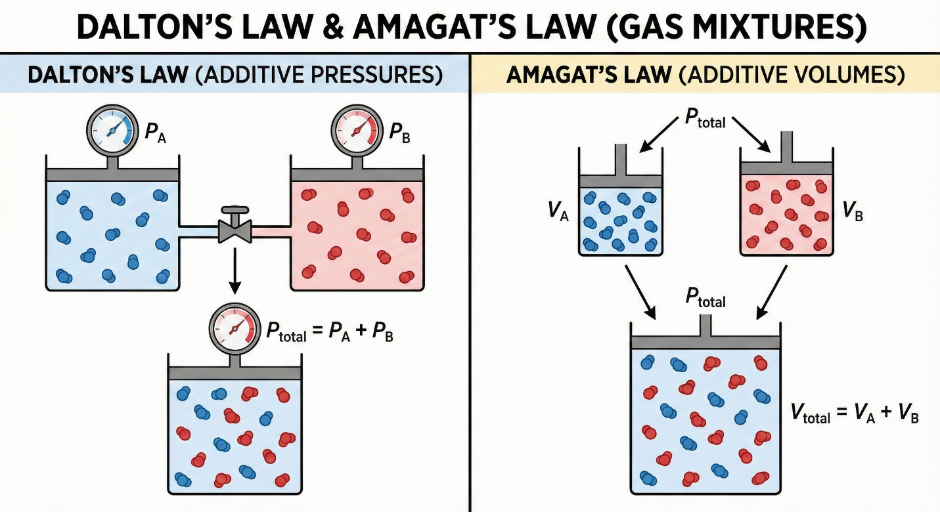
\includegraphics[width=4.27083in,height=2.32934in]{images/IntroToCHemEng2/media/image79.png}

מהחוקים הללו נגזרת אחת התכונות השימושיות ביותר של גזים אידיאלים - הזהות
המוחלטת בין יחסי המולים, הלחצים והנפחים. עבור גז \ul{אידיאלי} מתקיים
תמיד:

\[y_{i} = \frac{n_{i}}{n_{total}} = \frac{P_{i}}{P_{total}} = \frac{V_{i}}{V_{total}}\]

כך שאם נתון לנו הרכב של גז ב"אחוזים נפחיים" (למשל: אוויר מכיל 21\%
חמצן), ניתן להניח מיד שזהו גם אחוז המולים, וזהו גם אחוז הלחץ שהגז תורם.

::: \{.callout-note title="הערה חשובה"\}

זהות זו נכונה רק עבור גזים אידיאליים. בגזים ריאליים בלחצים גבוהים, אחוזי
הנפח אינם זהים בהכרח לאחוזי המולים עקב כוחות דחייה ומשיכה שונים בין
מולקולות שונות (נפח הערבוב אינו זניח).

:::

\subsection{סיכום -- גזים
אידיאליים}\label{ux5e1ux5d9ux5dbux5d5ux5dd-ux5d2ux5d6ux5d9ux5dd-ux5d0ux5d9ux5d3ux5d9ux5d0ux5dcux5d9ux5d9ux5dd}

\begin{itemize}
\item
  גז אידיאלי הוא מודל תיאורטי המתבסס על ההנחותש נפח המולקולות
  ואינטראקציות ביניהן מוזנחים. המודל אינו מדויק לחלוטין אך מתאים לרוב
  היישומים ההנדסיים בלחצים לא גבוהים ובטמפרטורות רחוקות מתנאי עיבוי.
\item
  משוואת הגז האידיאלי:
\end{itemize}

\[PV = nRT\] קושרת בין לחץ P, נפח \(V\), טמפרטורה מוחלטת \(T\) וכמות
חומר \(n\). שינוי באחד מחייב שינוי באחרים בהתאם לאילוצי המערכת.

\begin{itemize}
\tightlist
\item
  קבוע הגזים:
\end{itemize}

\[R = \frac{PV}{nT} = 8.314\frac{m^{3}\ Pa}{mol\ K} = \ 0.08206\ \frac{L\ atm}{mol\ K} = 10.73\frac{ft^{3}\ psi}{lb - mol\ \ {^\circ}R}\]

הוא יחס פיזיקלי קבוע; ערכו הנומרי תלוי במערכת היחידות. בשימוש בו אנו
חייבים להשתמש בטמפרטורה מוחלטת (K או \({^\circ}R\) (ובלחץ מוחלט.

\begin{itemize}
\tightlist
\item
  שימושים מרכזיים בהנדסת תהליכים:
\end{itemize}

\[{n = \frac{PV}{RT}\text{ (כמות גז ממיכל)}
}{\dot{n} = \frac{P\dot{V}}{RT}\text{(מעבר מספיקה נפחית לספיקה מולרית)}
}{\frac{P_{1}V_{1}}{T_{1}} = \frac{P_{2}V_{2}}{T_{2}}\text{(השוואה בין מצבים, }n = \text{קבוע)}
}\]

\begin{itemize}
\tightlist
\item
  ניתן לבדוק את תקפות ההנחה האידיאלית נבחנת לפי מידת הדילול של הגז. נפח
  מולרי אידיאלי:
\end{itemize}

\[\widehat{V} = \frac{RT}{P}\]

\begin{enumerate}
\def\labelenumi{\arabic{enumi}.}
\tightlist
\item
  עבור גזים פשוטים (דו-אטומיים ואצילים):
\end{enumerate}

\[{\widehat{V}}_{ideal} = \frac{RT}{P} \geq 5\frac{L}{mol}\ \ \ \ \ or\ \ \ {\widehat{V}}_{ideal} = \frac{RT}{P} \geq 80\frac{ft^{3}}{lbmol}\]

\begin{enumerate}
\def\labelenumi{\arabic{enumi}.}
\setcounter{enumi}{1}
\tightlist
\item
  עבור גזים אחרים (מורכבים):
\end{enumerate}

\[\ \ {\widehat{V}}_{ideal} = \frac{RT}{P} \geq 20\frac{L}{mol}\ \ \ \ \ {\widehat{V}}_{ideal} = \frac{RT}{P} \geq 320\frac{ft^{3}}{lbmol}\]

\begin{itemize}
\tightlist
\item
  בתערובות של גזים אידיאליים כל רכיב מתנהג באופן עצמאי: לפי חוק דלתון
  הלחץ הכולל הוא סכום הלחצים החלקיים, ולפי חוק אמגא הנפח הכולל הוא סכום
  הנפחים החלקיים.\\
\item
  באופן כללי כשאנחנו עובדים עם תערובות של גזים אידיאליים אפשר לראות
  שהשבר המולי שווה לשבר הנפחי ושווה לשבר הלחצים, וניתן לעשות מעבר זה
  באופן אוטומטי. **
  \[y_{i} = \frac{n_{i}}{n_{total}} = \frac{P_{i}}{P_{total}} = \frac{V_{i}}{V_{total}}\]
\end{itemize}

\section{גזים
ריאליים}\label{ux5d2ux5d6ux5d9ux5dd-ux5e8ux5d9ux5d0ux5dcux5d9ux5d9ux5dd}

עד כה ניתחנו מערכות גזיות תוך שימוש במשוואת הגז האידיאלי \(PV = nRT\)
אשר סיפקה תיאור פשוט ואפקטיבי של הקשר בין לחץ, נפח, טמפרטורה וכמות חומר.
כאשר אנו עובדים על לחצים מתונים וטמפרטורות שאינן קיצוניות חישוב זה נותן
לנו הערכה טובה ומאפשר חישוב מהיר ואינטואיטיבי של משתני תהליך. עם זאת,
ככל שתנאי התהליך מתרחקים מאזורים אלו, ובפרט בלחצים גבוהים או בטמפרטורות
נמוכות, ההתנהגות של גזים מתחילה לסטות מן האידיאליות. במצבים אלו, ההנחות
הבסיסיות של המודל האידיאלי, נפח זניח של המולקולות והיעדר אינטראקציות
ביניהן, אינן מתקיימות עוד, והשימוש במשוואת הגז האידיאלי עלול להוביל
לשגיאות חישוביות שאינן זניחות מבחינה הנדסית.

כאשר מתברר שמשוואת הגז האידיאלי אינה מספקת תוצאות מדויקות, עומדות
לרשותנו שתי אפשרויות עיקריות לפתרון. האפשרות הראשונה היא \textbf{שימוש
במשוואות מצב מתקדמות} - מודלים מתמטיים מורכבים יותר (תיאורטיים או
אמפיריים) שנועדו להחליף את המשוואה הפשוטה ולתאר בדיוק רב את פיזיקת
החלקיקים. האפשרות השנייה, והנפוצה מאוד בהנדסה, היא \textbf{תיקון המודל
הקיים.} במקום לעבור למשוואה חדשה ומסובכת, אנו שומרים על התבנית המוכרת
והנוחה של משוואת הגז האידיאלי, אך מוסיפים לה \textquotesingle גורם
תיקון\textquotesingle{} המפצה על הסטייה מההתנהגות האידיאלית. בפרק זה
נתחיל ביישום שיטת התיקון (מקדם הדחיסות), ובהמשך נכיר את המודלים המתקדמים
יותר לתיאור גזים ריאליים.

\subsection{מקדם הדחיסות
Z}\label{ux5deux5e7ux5d3ux5dd-ux5d4ux5d3ux5d7ux5d9ux5e1ux5d5ux5ea-z}

כדי להתמודד עם סטיות מהתנהגות אידיאלית של גזים, נרצה תחילה להרחיב את
משוואת הגז האידיאלי מבלי לנטוש אותה לחלוטין. הדרך הפשוטה והישירה לעשות
זאת היא להכניס גורם תיקון המתאר את הפער בין ההתנהגות האידיאלית לבין
ההתנהגות הנמדדת בפועל. גורם תיקון זה נקרא מקדם הדחיסות, ומסומן \(Z\).

מקדם הדחיסות מוגדר כיחס בין הנפח המולרי האמיתי של הגז
(\({\widehat{V}}_{real}\)), לבין הנפח שהיה מתקבל אילו הגז היה מתנהג
כאידיאלי באותם תנאי לחץ וטמפרטורה
(\({\widehat{V}}_{ideal} = RT\text{/}P\))

\[Z = \frac{{\widehat{V}}_{real}}{{\widehat{V}}_{ideal}} = \frac{P\widehat{V}}{RT}\]

באמצעות הגדרה זו, אנו יכולים לכתוב מחדש את משוואת המצב בצורה המתוקנת
הבאה:

\[P\widehat{V} = ZRT\quad\text{או}\quad PV = ZnRT\]

כאשר V הוא הנפח הכולל ו-n הוא מספר המולים. משוואה זו זהה בצורתה למשוואת
הגז האידיאלי, כאשר כל "חוסר האידיאליות" מקופל בתוך הפרמטר היחיד Z.

כאשר \(Z = 1\), מתקבלת בדיוק משוואת הגז האידיאלי, והמשמעות היא שהגז
מתנהג בקירוב אידיאלי בתנאי התהליך הנתונים. סטייה של \(Z\) מערך זה מעידה
על כך שהנפח המולרי של הגז שונה מן הנפח שהיה מתקבל אילו ההתנהגות הייתה
אידיאלית לחלוטין. כאשר \(Z \neq 1\), \(Z\) מייצג השפעה מצטברת של מספר
תופעות פיזיקליות הקשורות לכוחות משיכה ודחייה בין-מולקולריים ולנפח העצמי
של המולקולות. עם זאת, באופן כללי נתון להגיד שכאשר מתקבל \(Z < 1\), פירוש
הדבר הוא שהנפח המולרי האמיתי של הגז קטן מן הנפח האידיאלי הצפוי. מצב זה
מאפיין לרוב טמפרטורות בינוניות-נמוכות שבהן השפעת כוחות המשיכה בין
המולקולות בולטת יותר, כך שהגז ``דחוס'' יותר מכפי שמנבא המודל האידיאלי.
לעומת זאת, כאשר מתקבל \(Z > 1\) , הנפח המולרי גדול מן הערך האידיאלי,
תופעה הקשורה להשפעת הנפח העצמי של המולקולות ולדחייה קצרי־טווח ביניהן,
ונפוצה יותר בלחצים גבוהים.

אבל כיצד נמצא את ערך של Z? הערך של Z אינו קבוע; הוא משתנה עבור כל גז,
ותלוי בטמפרטורה ובלחץ הספציפיים שבהם הוא נמצא. כיצד ניתן לקבוע את Z עבור
גז נתון בתנאי לחץ וטמפרטורה נתונים? כדי לאפשר הכללה, נשתמש בתכונות
קריטיות ובחוק המצבים התואמים, שמאפשרים להעריך \(Z\)עבור גזים שונים
באמצעות משתנים חסרי מימד. כדי להבין זאת, נחזור בקצרה לדיאגרמת הפאזות
(P-T diagram) המוכרת ונחדד מספר הגדרות חשובות שישמשו אותנו בחישובים.

\href{../../projects/IntrotoProcessEngineering/simulations/phase.html}{..\textbackslash..\textbackslash projects\textbackslash IntrotoProcessEngineering\textbackslash simulations\textbackslash phase.html}

דיאגרמת פאזות מתארת אילו מצבי חומר יציבים עבור ערכי לחץ וטמפרטורה שונים.
בדיאגרמה זו ניתן לראות שעקומת שיווי-המשקל בין נוזל לגז (עקומת הרתיחה)
אינה נמשכת עד אינסוף. היא מסתיימת בנקודה ספציפית הנקראת הנקודה הקריטית.

טמפרטורה קריטית \(T_{c}\) -הטמפ\textquotesingle{} הגבוהה ביותר שבה החומר
יכול להתקיים במצב צבירה נוזלי, מעל לטמפ\textquotesingle{} זו האנרגיה
הקינטית של המולקולות גבוהה מדי מכדי שכוחות המשיכה יחזיקו אותן יחד כנוזל,
לא משנה כמה לחץ נפעיל עליהן.

לחץ קריטי \(P_{c}\) - הלחץ הדרוש על מנת לנזל את הגז בדיוק
בטמפ\textquotesingle{} הקריטית שלו

תכונה חשובה אחת היא ההבחנה בין גז לאדים. למרות שבשפת היום-יום אנו
משתמשים במונחים "גז" ו"אדים" בערבוביה, בהנדסת תהליכים ישנה אבחנה ברורה
ביניהם.

אדים - חומר במצב גזי הנמצא מתחת לטמפ\textquotesingle{} הקריטית שלו
\(T < T_{c}\), והאדים ניתנים לעיבוי על ידי הפעלת לחץ בלבד (דחיסה
איזורתמית).

גז -- חומר במצב גזים מעל הטמפ\textquotesingle{} הקריטית \(T > T_{c}\),
הגז אינו ניתן לעיבוי על ידי העלאת הלחץ בלבד.

בקרבת הנקודה הקריטית ההבדל בין נוזל לגז ``מיטשטש'', ותכונות החומר משתנות
באופן רגיש במיוחד לתנאים. למצב צבירה זה אנו קוראים זורם סופר קריטי

\textbf{זורם סופר-קריטי (Supercritical Fluid):} מצב שבו החומר נמצא מעל
הטמפרטורה הקריטית\\
(\(T > T_{c}\)) ומעל הלחץ הקריטי (\(P > P_{c}\)). לחומר יש צפיפות גבוהה
המזכירה נוזל, אך צמיגות נמוכה ויכולת דיפוזיה המזכירה גז. (תכונות אלו
הופכות אותו לממס מצוין בתעשייה, למשל במיצוי קפאין מפולי קפה).

אולם חשיבותם של הערכים הקריטיים
(\(\mathbf{T}_{\mathbf{c}}\mathbf{,}\mathbf{P}_{\mathbf{c}}\)) חורגת
מעבר להגדרת מצבי הצבירה. נקודות ציון פנימיות אלו מספקות לנו את המפתח
להשוואה אמיתית בין חומרים שונים. האם יש קשר בין ההתנהגות של גזים שונים?
במבט ראשון, נראה שהתשובה היא לא. אם נשרטט גרף של מקדם הדחיסות (Z) כתלות
בלחץ עבור מגוון גזים בטמפרטורה אחידה יראה כאילו כל גז מתנהג אחרת לגמרי:
גז אחד נדחס מאוד (Z יורד תלולות), אחר כמעט ולא משתנה, ושלישי בכלל מראה
סטייה חיובית. נדמה שאין שום דרך לחזות התנהגות של גז אחד על סמך גז אחר.
אך כשמסתכלים לעומק ניתן לראות שהמבנה הכללי של העקומות דומה עבור כל
הגזים, הגרף מתחיל ב\(z = 1\) בלחץ אפס. ככל שמעלים את הלחץ, ברוב המקרים
הגרף יורד תחילה (השפעת כוחות משיכה) ואז, בלחצים גבוהים יותר, עולה
בתלילות כלפי מעלה (השפעת כוחות דחייה).

\begin{tcolorbox}[enhanced jigsaw, colback=white, arc=.35mm, coltitle=black, breakable, toptitle=1mm, leftrule=.75mm, colbacktitle=quarto-callout-note-color!10!white, opacitybacktitle=0.6, bottomtitle=1mm, titlerule=0mm, opacityback=0, colframe=quarto-callout-note-color-frame, title={הערה}, rightrule=.15mm, bottomrule=.15mm, toprule=.15mm, left=2mm]

\#\#\# איור 5.4.1: סימולציה אינטראקטיבית -- מקדם הדחיסות (\$z\$) כתלות
בלחץ ובטמפרטורה

\textless iframe src="real-gas.html" width="100\%" height="600px"
style="border:none;"\textgreater\textless/iframe\textgreater{}

**שאלות מנחות לחקירה:**

\begin{enumerate}
\def\labelenumi{\arabic{enumi}.}
\item
  **הגבול של לחץ נמוך:** הציבו את המחוון על טמפרטורה כלשהי. מהו ערכו של
  \$z\$ כאשר הלחץ מתקרב ל-0 אטמוספירות? האם ערך זה משתנה כשמחליפים בין
  הגזים השונים?
\item
  **השפעת הטמפרטורה:** בחרו את הגז **מתאן (\$CH\_4\$)**. התחילו
  בטמפרטורה נמוכה (סביב \$200K\$) והעלו אותה בהדרגה ל-\$500K\$. כיצד
  משפיעה העלאת הטמפרטורה על הסטייה מהתנהגות אידיאלית (\$z=1\$)?
\item
  **השוואה בין חומרים:** קבעו את הטמפרטורה על \$300K\$. החליפו בין
  **חנקן (\$N\_2\$)** לבין **פחמן דו-חמצני (\$CO\_2\$)**. איזה מהגזים
  מציג סטייה גדולה יותר מאידיאליות בטמפרטורה זו, ומדוע? (רמז: בדקו את
  הערך של \$T\_c\$ המוצג עבור כל גז).
\item
  **מעבר פאזה:** בחרו ב**מים (\$H\_2O\$)** והורידו את הטמפרטורה אל מתחת
  ל-\$647K\$. מה קורה לצורת הגרף בלחצים נמוכים? (הלולאה שנוצרת מייצגת את
  אזור הדו-פאזי שבו הגז מתעבה לנוזל, כפי שמתואר במשוואת ואן-דר-ואלס).
\end{enumerate}

\end{tcolorbox}

הדמיון הזה במבנה מרמז לנו שהפיזיקה הבסיסית הפועלת על מולקולות חמצן היא
אותה פיזיקה הפועלת על מולקולות מתאן. ההבדל ביניהן הוא לא ב"חוקים", אלא
ב"סקאלה" -- בעוצמת הכוחות הפנימיים האופיינית לכל חומר. הבעיה בהשוואה
הקודמת הייתה שהשתמשנו ב"סרגל מדידה" אבסולוטי (למשל, אטמוספירות וקלווין)
עבור חומרים שהסקאלה הפנימית שלהם שונה לחלוטין. טמפרטורה של \(300K\)
נחשבת "לוהטת" עבור חנקן (הנמצא הרבה מעל הטמפרטורה הקריטית שלו) אך
"קפואה" עבור מים (הנמצאים עמוק מתחתיה). לא הוגן להשוות ביניהם באותם
תנאים. כדי למצוא את החוקיות במקום לשאול "מה הלחץ?" נשאל "עד כמה הלחץ הזה
גבוה ביחס ללחץ הקריטי של החומר הספציפי?"

חוק המצבים התואמים (Law of Corresponding States)- החוק קובע שאם מנרמלים
את התנאים ומסתכלים על הלחץ והטמפרטורה באופן יחסי לנקודה הקריטית של כל
חומר, ניתן "ליישר" את התנהגות הגזים לפי עקומה אחת אוניברסלית.

\subsubsection{משתנים מופחתים (Reduced
Variables)}\label{ux5deux5e9ux5eaux5e0ux5d9ux5dd-ux5deux5d5ux5e4ux5d7ux5eaux5d9ux5dd-reduced-variables}

כדי ליישם את חוק המצבים התואמים ולהשוות בין חומרים שונים, עלינו לתרגם את
תנאי התהליך שלנו לערכים יחסיים, חסרי יחידות. ערכים אלו נקראים
\textbf{משתנים מופחתים}:

\[T_{r} = \frac{T}{T_{c}}\quad,\quad P_{r} = \frac{P}{P_{c}}\]

משתנים אלו מבטאים עד כמה הטמפרטורה והלחץ רחוקים מן הערכים הקריטיים
האופייניים לחומר הנדון. באופן זה, שני גזים שונים הנמצאים באותו \(T_{r}\)
ואותו \(P_{r}\)נמצאים במצב פיזיקלי דומה מבחינת ``המרחק היחסי'' שלהם מן
הנקודה הקריטית, גם אם הערכים המוחלטים של \(T\ \)ו \(P\)-שונים לחלוטין.
באמצעות המשתנים המופחתים וגרפי הדחיסות הכלליים אנו יכולים להעריך את ערכו
של מקדם הדחיסות Z עבור גזים ריאליים.

הגרפים הבאים מציגים את ההתנהגות הכללית של פקטור הדחיסות \(Z\) כפונקציה
של לחץ וטמפרטורה מוקטנים. לצורכי המחשה והבנה, הגרפים חושבו באמצעות
משוואת מצב של גז אמיתי, המשחזרת את המאפיינים הפיזיקליים העיקריים של
ההתנהגות הנמדדת.

\begin{figure}[H]

{\centering 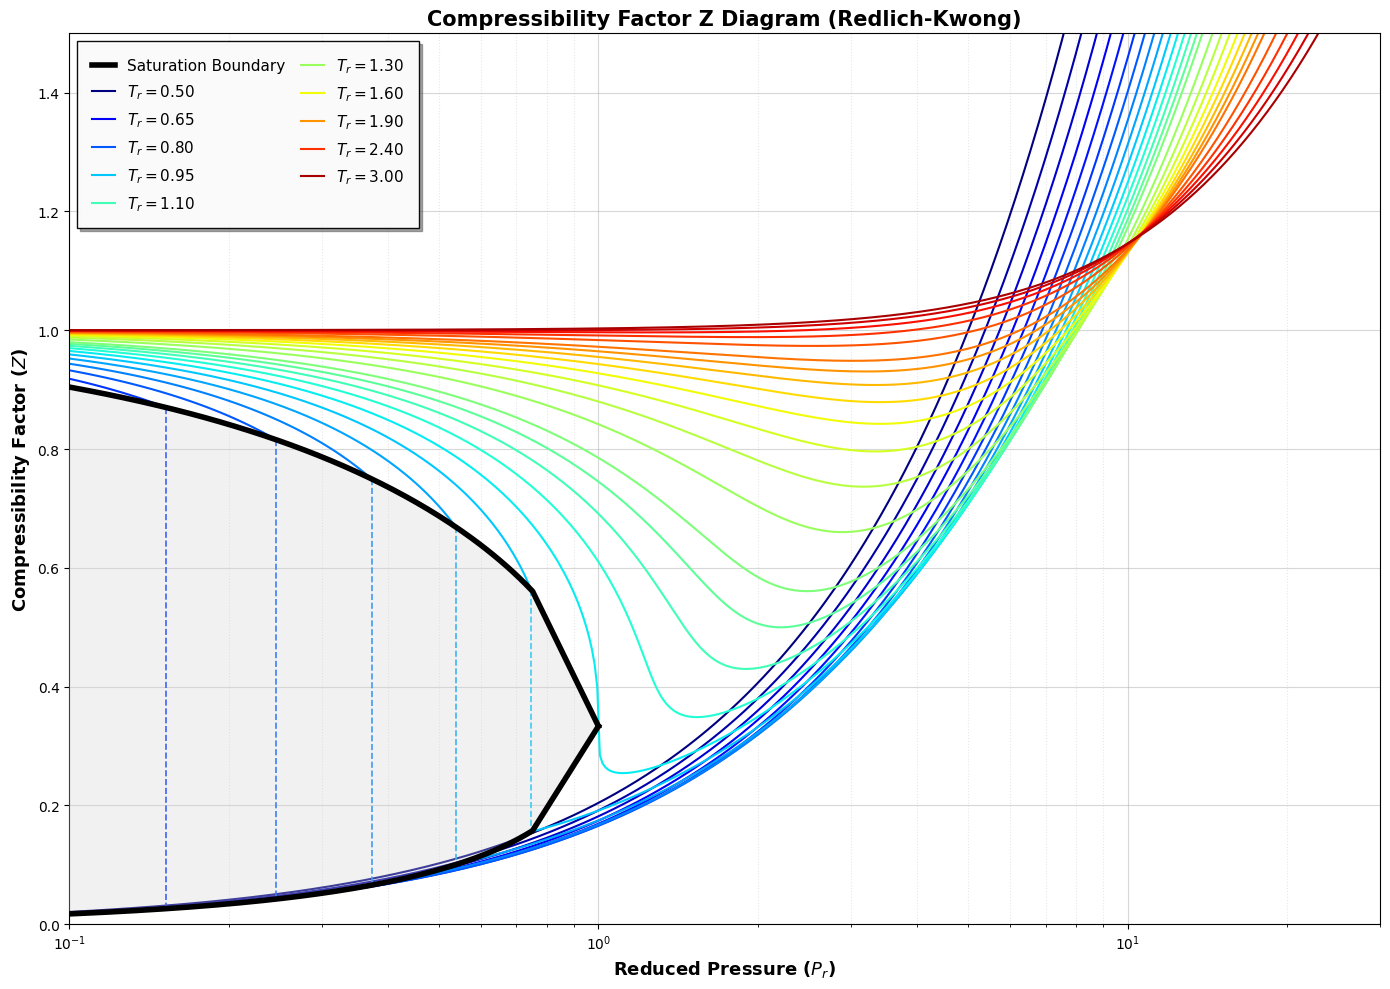
\includegraphics[width=6.35417in,height=4.51927in]{images/IntroToCHemEng2/media/image80.png}

}

\caption{Figure 35 - הגרף מציג את פקטור הדחיסות \(Z\) כפונקציה של הלחץ
המוקטן \(P_{r}\)עבור טמפרטורות מוקטנות שונות \(T_{r}\). כל עקומה מייצגת
איזותרמה. בלחצים נמוכים מתקבל \(Z \approx 1\), המעיד על התנהגות קרובה
לגז אידיאלי. עבור טמפרטורות נמוכות מופיעה סטייה משמעותית מגז אידיאלי,
המתבטאת בשקע ב-\(Z\) וקשורה לכוחות משיכה בין המולקולות. הקו השחור מתאר
את גבול הרוויה (אזור דו־פאזי- שיווי משקל בין נוזל לגז).}

\end{figure}%

\begin{figure}[H]

{\centering 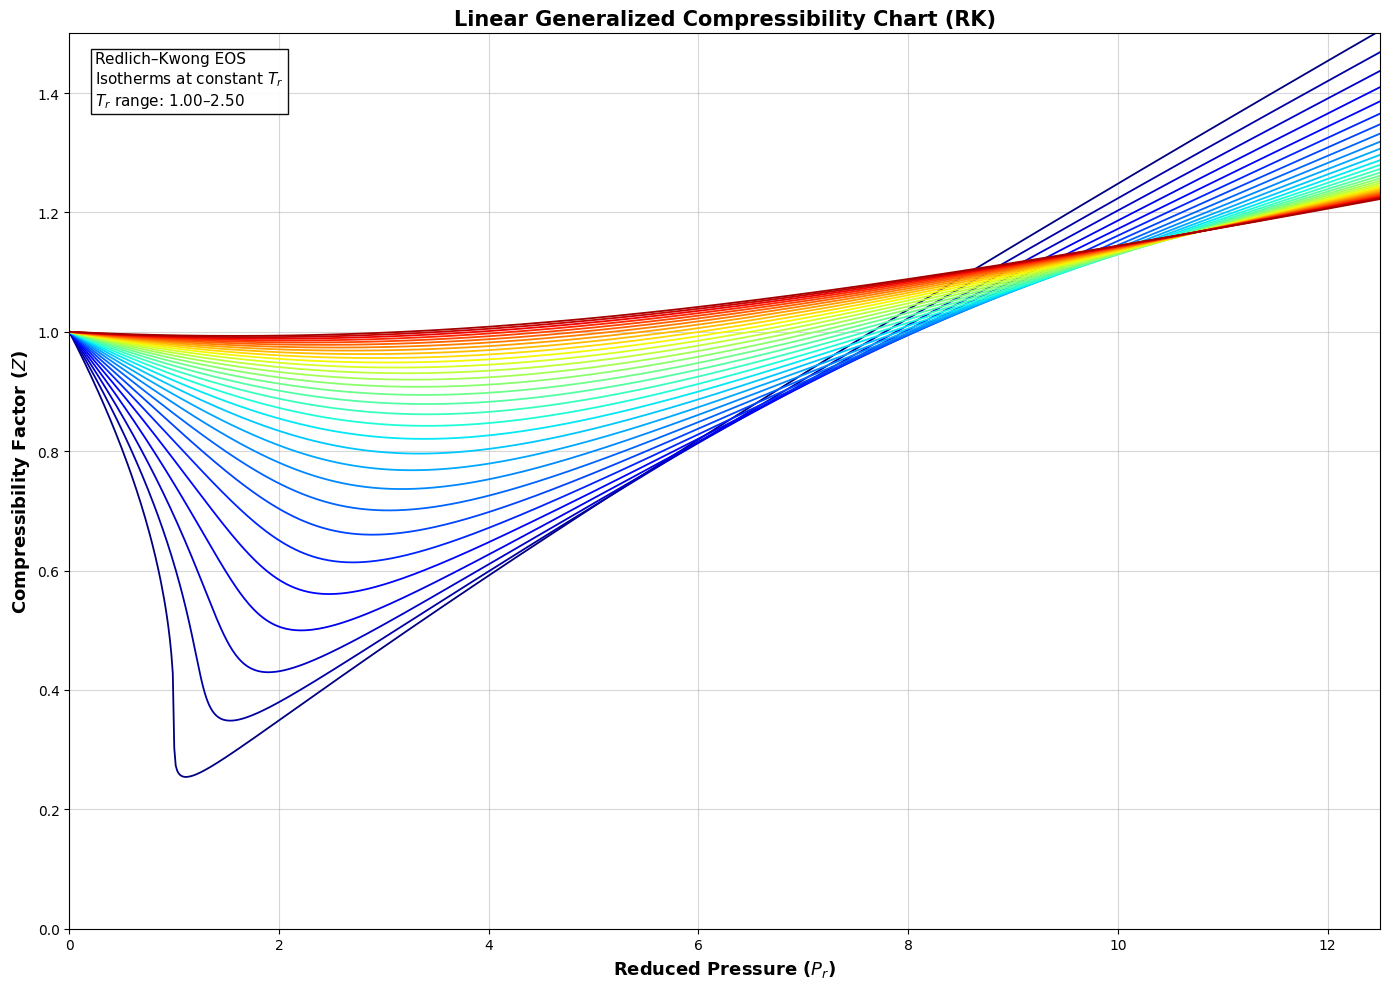
\includegraphics[width=6.49306in,height=4.61806in]{images/IntroToCHemEng2/media/image81.png}

}

\caption{Figure 36 - פקטור הדחיסות \(Z\) \textbf{כתלות בלחץ מוקטן}
\(P_{r}\) \textbf{עבור איזותרמות שונות, מחושב לפי משוואת המצב
Redlich--Kwong.}}

\end{figure}%

הגרפים המוצגים כאן מתארים את ההתנהגות הכללית של פקטור הדחיסות \(Z\)
כפונקציה של לחץ וטמפרטורה מוקטנים. גרפים קלאסיים מסוג זה מבוססים במקור
על אוסף רחב של נתונים אמפיריים שנמדדו עבור גזים שונים, ואשר עובדו לגרפים
מוכללים (Generalized Compressibility Charts). במסגרת ספר זה, לצורכי
הדגמה, הבנה ויצירת גרפים רציפים ונשלטים, ההתנהגות מחושבת באמצעות משוואת
מצב של גז אמיתי (Redlich--Kwong). השימוש במודל מאפשר לשחזר את המאפיינים
הפיזיקליים העיקריים של הגרפים האמפיריים, כגון סטייה מגז אידיאלי, הופעת
אזור דו־פאזי, והתנהגות חריגה בקרבת הנקודה הקריטית\textbf{. להצגה מדוייקת
יותר המבוססת ישירות על נתונים אמפיריים, ראו איור 5.4 אצל Felder et
al.~(2016).}

\subsubsection{שימוש בגרף הדחיסות הכללי -- הלכה
למעשה}\label{ux5e9ux5d9ux5deux5d5ux5e9-ux5d1ux5d2ux5e8ux5e3-ux5d4ux5d3ux5d7ux5d9ux5e1ux5d5ux5ea-ux5d4ux5dbux5dcux5dcux5d9-ux5d4ux5dcux5dbux5d4-ux5dcux5deux5e2ux5e9ux5d4}

נניח, לשם הדגמה, כי נתונים לנו הלחץ (P) והטמפרטורה (T) של גז מסוים, ואנו
מעוניינים לחשב את הנפח המולרי שלו (\(\widehat{V}\)).

\textbf{1. נמצא} את הערכים הקריטיים של הגז הספציפי - הטמפרטורה הקריטית
\(T_{c}\)והלחץ הקריטי \(P_{c}\) מתוך טבלאות תרמודינמיות או נספחים בספר
הקורס.

\textbf{2. נחשב} את הטמפרטורה והלחץ המופחתים:

\[T_{r} = \frac{T}{T_{c}},P_{r} = \frac{P}{P_{c}}\]

\textbf{3. בגרף הדחיסות הכללי}\\
- נאתר את הערך של \(P_{r}\) על ציר ה -- \(x\).

\begin{itemize}
\item
  נעלה אנכית עד למפגש עם האיזותרמה המתאימה ל- \(T_{r}\).
\item
  אם הערך המדויק של \(T_{r}\) אינו מופיע, נעשה אינטרפולציה ויזואלית בין
  העקומות.
\item
  נקרא את ערך מקדם הדחיסות \(Z\) מציר ה־\(y\).
\end{itemize}

\textbf{4. נציב את} \(Z\) במשוואת המצב המתוקנת ונחשב את הנפח המולרי:

\[\widehat{V} = \frac{ZRT}{P}\]

חישוב נפח גז חנקן בלחץ גבוה

נתונים שני מיכלים המכילים גז חנקן (\(N_{2}\)) בטמפרטורה של
\(200\,\text{K}\) הראשון בלחץ של \(1\,\text{atm}\) והשני בלחץ של
\(100atm\). חשבו את הנפח המולרי של הגז בשני המיכלים בשתי דרכים:\\
א. בהנחת גז אידיאלי.\\
ב. באמצעות גרף הדחיסות הכללי (גז ריאלי).

פתרון

חלק א': הנחת גז אידיאלי (\(\mathbf{Z} = \mathbf{1}\))

עבור המיכל הראשון

\[{\widehat{V}}_{ideal} = \frac{RT}{P} = \frac{0.08206\ \frac{L\ atm}{mol\ K}\ 200K}{1atm} = 16\frac{L}{mol}\]

\[{\widehat{V}}_{ideal} = \frac{RT}{P} = \frac{0.08206\ \frac{L\ atm}{mol\ K}\ 200K}{100atm} = 0.16\frac{L}{mol}\]

חלק ב': שימוש בגרף הדחיסות

נתונים קריטיים לחנקן (מתוך טבלת נתונים) -
\(T_{c} = 126.2K,\ P_{c} = 33.5atm\)

חישוב טמפקטורה מופחתת (עבור שני המיכלים)
\(T_{r} = \frac{200K}{126.2K} \approx 1.58\)

עבור המיכל הראשון

נחשב לחץ מופחת

\[\ \ \ \ P_{r} = \frac{1atm}{33.5atm} \approx 0.03\]

ובגרף הדחיסות הכללי עבור \(P_{r} \ll 1\) מתקבל \(Z = 1\)

\[{\widehat{V}}_{ideal} = Z\frac{RT}{P} = 1*\frac{0.08206\ \frac{L\ atm}{mol\ K}\ 200K}{1atm} = 0.16\frac{L}{mol}\]

וניתן לראות שבלחצים נמוכים הגז מתנהג כגז אידיאלי.

עבור המיכל השני

\[P_{r} = \frac{100}{33.5} \approx 2.98\]

ובגרף הדחיסות ניתן לראות שעבור \(P_{r} \approx 3,\ T_{r} \approx 1.6\)
מתקבל בקירוב \(Z \approx 0.86\)

\[{\widehat{V}}_{real} = Z\frac{RT}{P} = 0.86 \cdot \frac{0.08206\frac{L\ atm}{mol\ K} \cdot 200K}{100atm} = 0.14\]

\begin{longtable}[]{@{}
  >{\raggedright\arraybackslash}p{(\linewidth - 6\tabcolsep) * \real{0.0743}}
  >{\raggedright\arraybackslash}p{(\linewidth - 6\tabcolsep) * \real{0.1284}}
  >{\raggedright\arraybackslash}p{(\linewidth - 6\tabcolsep) * \real{0.3919}}
  >{\raggedright\arraybackslash}p{(\linewidth - 6\tabcolsep) * \real{0.3919}}@{}}
\toprule\noalign{}
\begin{minipage}[b]{\linewidth}\raggedright
\textbf{מיכל}
\end{minipage} & \begin{minipage}[b]{\linewidth}\raggedright
\textbf{לחץ (atm)}
\end{minipage} & \begin{minipage}[b]{\linewidth}\raggedright
\[{\widehat{V}}_{ideal}\ \left( \frac{L}{mol} \right)\]
\end{minipage} & \begin{minipage}[b]{\linewidth}\raggedright
\[{\widehat{V}}_{real}\ \left( \frac{L}{mol} \right)\]
\end{minipage} \\
\midrule\noalign{}
\endhead
\bottomrule\noalign{}
\endlastfoot
1 & 1 & 16.41 & 16.41 \\
2 & 100 & 0.164 & 0.141 \\
\end{longtable}

במיכל הראשון אין הבדל מעשי בין המודלים -- הסטייה מאידיאליות זניחה.\\
במיכל השני, לעומת זאת, הנפח המולרי האמיתי קטן בכ־14--16\% מהערך
האידיאלי, עקב השפעת כוחות משיכה בין־מולקולריים בלחץ גבוה.

ההליך שתואר עד כה מתאים במיוחד למצבים שבהם הנעלם הוא הנפח V. אולם לעיתים
נתון לנו נפח המיכל וכמות החומר, ואנו נדרשים לחשב דווקא את הלחץ P. במקרה
כזה נוצרת תלות מעגלית: כדי למצוא את Zמהגרף יש לדעת את הלחץ המופחת
\(P_{r}\), אך \(P_{r}\)עצמו תלוי בלחץ:

\[P_{r} = \frac{P}{P_{c}} = \frac{ZnRT/V}{P_{c}}\] מצבים כאלה נפוצים
מאוד בעבודה הנדסית, והפתרון המקובל להם הוא שימוש בתהליך איטרטיבי פשוט.

\textbf{שיטת הפתרון (איטרציה)}

\begin{itemize}
\item
  מנחשים ערך התחלתי ל\(Z\) (בדרך כלל Z=1 כלומר התחלה מגז אידיאלי).
\item
  מחשבים את הלחץ P לפי הניחוש.
\item
  מחשבים את \(P_{r}\) המתאים.
\item
  ניגשים לגרף ומוצאים את ערך \(Z\) עבור \(P_{r}\) ו־\(T_{r}\).
\item
  אם ערך Z שנקרא מהגרף קרוב לערך שניחשנו -- הפתרון הושג.
\item
  אם לא, משתמשים בערך Z החדש כניחוש לסיבוב הבא וחוזרים על התהליך עד
  להתכנסות.
\end{itemize}

מיכל קשיח מכיל גז חנקן (\(N_{2}\)) בטמפרטורה \(T = 200\text{ }K\). הנפח
המולרי של הגז במיכל נמדד כ:

\[\widehat{V} = 0.200\ L/mol\] חשבו את הלחץ \(P\)של הגז בשתי דרכים:\\
א. בהנחת גז אידיאלי.\\
ב. כגז ריאלי באמצעות גרף הדחיסות הכללי

** א. עבור גז אידיאלי (\(Z = 1\))

\[P_{ideal} = \frac{RT}{\widehat{V}} = \frac{0.08206\frac{L\ atm}{mol\ K} \cdot 200K}{0.200\ L/mol} = 82\text{ }atm\]
ב. כגז ריאלי

נתונים קריטיים לחנקן: \(T_{c} = 126.2\text{ , }P_{c} = 33.5\text{ }atm\)

שלב 1: מחשבים \(\mathbf{T}_{\mathbf{r}}\) (קבוע לכל האיטרציות)

\[\mathbf{T}_{\mathbf{r}} = \frac{\mathbf{T}}{\mathbf{T}_{\mathbf{c}}} = \frac{\mathbf{200}}{\mathbf{126}.\mathbf{2}} \approx \mathbf{1}.\mathbf{6}\]

שלב 2: איטרציה על \(\mathbf{Z}\)

מנחשים \(\mathbf{Z}\) \textbf{←} מחשבים
\(\mathbf{P} = \frac{\mathbf{ZRT}}{\widehat{\mathbf{V}}}\) ← מחשבים
\(\mathbf{P}_{\mathbf{r}} = \frac{\mathbf{P}}{\mathbf{P}_{\mathbf{c}}}\)
← קוראים \(\mathbf{Z}\) מהגרף עבור
\(\left( \mathbf{T}_{\mathbf{r}},\mathbf{P}_{\mathbf{r}} \right)\) ←
חוזרים על התהליך עד שהתוצאה מתייצבת

נגדיר קבוע נוח:

\[P_{ideal} = \ \frac{RT}{\widehat{V}} = \frac{0.08206\frac{L\ atm}{mol\ K} \cdot 200K}{0.200L/mol} = 82atm\]
ולכן:

\[P(atm) = Z \cdot P_{ideal}(atm)\]

טבלת איטרציות

\begin{longtable}[]{@{}
  >{\raggedright\arraybackslash}p{(\linewidth - 8\tabcolsep) * \real{0.0556}}
  >{\raggedright\arraybackslash}p{(\linewidth - 8\tabcolsep) * \real{0.0992}}
  >{\raggedright\arraybackslash}p{(\linewidth - 8\tabcolsep) * \real{0.2897}}
  >{\raggedright\arraybackslash}p{(\linewidth - 8\tabcolsep) * \real{0.4048}}
  >{\raggedright\arraybackslash}p{(\linewidth - 8\tabcolsep) * \real{0.1429}}@{}}
\toprule\noalign{}
\begin{minipage}[b]{\linewidth}\raggedright
\textbf{איטרציה}
\end{minipage} & \begin{minipage}[b]{\linewidth}\raggedright
\textbf{ניחוש} \(\mathbf{Z}\)
\end{minipage} & \begin{minipage}[b]{\linewidth}\raggedright
\[\mathbf{P(atm) = Z \cdot}\mathbf{P}_{\mathbf{ideal}}\mathbf{(atm)}\]
\end{minipage} & \begin{minipage}[b]{\linewidth}\raggedright
\[\mathbf{P}_{\mathbf{r}}\mathbf{=}\frac{\mathbf{P}\left( \mathbf{atm} \right)}{\mathbf{33.5atm}}\]
\end{minipage} & \begin{minipage}[b]{\linewidth}\raggedright
\(\mathbf{Z}\) \textbf{חדש מהגרף (בערך)}
\end{minipage} \\
\midrule\noalign{}
\endhead
\bottomrule\noalign{}
\endlastfoot
0 & 1.00 & 82 & 2.45 & 0.88 \\
1 & 0.88 & 72.2 & 2.15 & 0.90 \\
2 & 0.90 & 73.9 & 2.21 & 0.90 \\
\end{longtable}

וניתן לראות שהפתרון מתכנס
ל-\(\mathbf{Z} \approx \mathbf{0}.\mathbf{90},\mathbf{P} \approx \mathbf{74}\text{ }\mathbf{atm}\)**

ניתן לראות כי הנחת הגז האידיאלי הייתה מעריכה את הלחץ בגז בכ10\% יותר.

\subsubsection{חישוב תכונות תערובת גזים באמצעות פקטור הדחיסות (Kay's
Rule)}\label{ux5d7ux5d9ux5e9ux5d5ux5d1-ux5eaux5dbux5d5ux5e0ux5d5ux5ea-ux5eaux5e2ux5e8ux5d5ux5d1ux5ea-ux5d2ux5d6ux5d9ux5dd-ux5d1ux5d0ux5deux5e6ux5e2ux5d5ux5ea-ux5e4ux5e7ux5d8ux5d5ux5e8-ux5d4ux5d3ux5d7ux5d9ux5e1ux5d5ux5ea-kays-rule}

כיצד ניתן להעריך את מקדם הדחיסות \(Z\ \)עבור תערובת גזים, כאשר לכל רכיב
בתערובת ערכים קריטיים שונים? גישה נפוצה ופשוטה, המתאימה ליישומים הנדסיים
רבים, היא כלל קיי (Kay's Rule). לפי כלל זה, ניתן להתייחס אל תערובת הגזים
כאילו הייתה ``גז מדומה'' יחיד, אשר תכונותיו הקריטיות מחושבות כממוצע
משוקלל של התכונות הקריטיות של רכיביה. תכונות אלו נקראות תכונות
פסאודו־קריטיות.

הטמפרטורה הפסאודו־קריטית של התערובת מוגדרת כ:

\[T_{c,\text{mix}} = \sum_{i}^{}y_{i}\text{ }T_{c,i}\] והלחץ
הפסאודו־קריטי מוגדר כ:

\[P_{c,\text{mix}} = \sum_{i}^{}y_{i}\text{ }P_{c,i}\]

כאשר \(y_{i}\) הוא השבר המולי של רכיב \(i\) בתערובת, ו-\(T_{c,i}\)
ו-\(P_{c,i}\) הם הערכים הקריטיים של אותו רכיב טהור.

לאחר חישוב הערכים הפסאודו־קריטיים, ממשיכים בדיוק כפי שנעשה עבור גז טהור:
מחשבים את המשתנים המופחתים של התערובת,

\[T_{r} = \frac{T}{T_{c,\text{mix}}},P_{r} = \frac{P}{P_{c,\text{mix}}}\]

קוראים את ערך מקדם הדחיסות \(Z\) מתוך גרף הדחיסות הכללי עבור ערכים אלו
ומציבים במשוואת המצב

\begin{quote}
\[V_{total} = \frac{Zn_{total}RT}{P}\]
\end{quote}

\begin{tcolorbox}[enhanced jigsaw, colback=white, arc=.35mm, coltitle=black, breakable, toptitle=1mm, leftrule=.75mm, colbacktitle=quarto-callout-tip-color!10!white, opacitybacktitle=0.6, bottomtitle=1mm, titlerule=0mm, opacityback=0, colframe=quarto-callout-tip-color-frame, title=\textcolor{quarto-callout-tip-color}{\faLightbulb}\hspace{0.5em}{עצה}, rightrule=.15mm, bottomrule=.15mm, toprule=.15mm, left=2mm]

\textbf{מתי כלל קיי עובד?}

כלל קיי הוא קירוב לינארי פשוט. הוא מספק דיוק טוב (שגיאה של אחוזים
בודדים) עבור תערובות של גזים בעלי מבנה כימי דומה (למשל תערובת של גזים
אינרטיים או סדרה הומולוגית של פחמימנים). עבור תערובות של גזים שונים מאוד
באופיים (למשל מולקולות קוטביות מאוד מעורבבות עם לא-קוטביות), הדיוק של
הכלל יורד, אך בקורס מבוא זה הוא ישמש אותנו ככלי העיקרי לפתרון בעיות
בתערובות.

\end{tcolorbox}

תערובת גזים מכילה \(80\%\) חנקן (\(N_{2}\)) ו- \(20\%\) פחמן דו־חמצני
(\(CO_{2}\)) (שברים מולריים). התערובת נמצאת בטמפרטורה \(T = 300\,\)
ובלחץ \(P = 50\, atm\). חשבו את הנפח המולרי הריאלי של התערובת.

נוציא נתונים קריטיים מהטבלה

חנקן - \(T_{c} = 126.2\text{ , }P_{c} = 33.5atm\)

פחמן דו חמצני \(T_{c} = 304.2K\text{ , }P_{c} = 73.8\ atm\)

השברים המולריים בתערובת:

\[y_{N_{2}} = 0.80,y_{CO_{2}} = 0.20\]

נחשב תכונות פסאודו־קריטיות (Kay's Rule)

טמפרטורה פסאודו־קריטית
\(T_{c,\text{mix}} = \sum_{i}^{}y_{i}T_{c,i} = 0.80 \cdot 126.2K + 0.20 \cdot 304.2K = 161K\)\emph{*
לחץ פסאודו־קריטי:
\(P_{c,\text{mix}} = \sum_{i}^{}y_{i}P_{c,i} = 0.80 \cdot 33.5atm + 0.20 \cdot 73.8atm = 41.6atm\)}*

נחשב משתנים מופחתים

\[{T_{r} = \frac{T}{T_{c,\text{mix}}} = \frac{300K}{161.8K} \approx 1.85
}{P_{r} = \frac{P}{P_{c,\text{mix}}} = \frac{50atm}{41.56atm} \approx 1.20
}\]

ניגש לגרף הדחיסות הכללי ונאתר את \(P_{r} \approx 1.2\). עולים עד
האיזותרמה המתאימה ל - \(T_{r} \approx 1.85\)\\
קריאה מהגרף נותנת בקירוב:

\[Z \approx 0.95\]

ולכן הנפח המולרי של התערובת יהיה

\[\widehat{V} = \frac{ZRT}{P} = \frac{0.95 \cdot 0.08206\frac{L\ atm}{mol\ K} \cdot 300K}{50atm} = 0.47\ L/mol\]

\subsection{משוואות מצב של גזים
ריאליים}\label{ux5deux5e9ux5d5ux5d5ux5d0ux5d5ux5ea-ux5deux5e6ux5d1-ux5e9ux5dc-ux5d2ux5d6ux5d9ux5dd-ux5e8ux5d9ux5d0ux5dcux5d9ux5d9ux5dd}

עד כה, הפתרון שלנו לסטייה מאידיאליות התבסס על גישה גרפית-אמפירית: השימוש
במקדם הדחיסות (\(\mathbf{Z}\)) ובחוק המצבים התואמים. גישה זו מצוינת
להבנה אינטואיטיבית ולחישובים ידניים מהירים, שכן היא "מנרמלת" את התנהגות
כל הגזים לתמונה ויזואלית אחת. אולם, לשיטה הגרפית ישנן מגבלות. קריאה
מגרפים חשופה לשגיאות אנוש, היא אינה נוחה לשימוש בתוכנות מחשב ובסימולציות
הנדסיות, והדיוק שלה מוגבל על ידי איכות הגרף והיכולת שלנו לבצע
אינטרפולציה. יתרה מכך, כאשר אנו נדרשים לבצע חישובים מורכבים יותר (כגון
חישובי שיווי-משקל פאזות או נגזרות תרמודינמיות), אנו זקוקים לביטוי מתמטי
רציף ומדויק, ולא רק לערך נקודתי מתוך גרף. כאן נכנסות לתמונה משוואות המצב
(Equations of State - EOS).

קיימות שתי גישות עיקריות לפיתוח משוואות מצב לגזים ריאליים. הגישה
הוויראלית מתארת את הסטייה מהתנהגות אידיאלית באמצעות פיתוח סדרתי של מקדם
הדחיסות בתחום תנאים נתון, ולכן היא מדויקת בעיקר בלחצים נמוכים ומתאימה
לניתוח תיאורטי. הגישה הקובית, לעומת זאת, בונה משוואת מצב סגורה אחת
הכוללת תיקונים פשוטים לדחייה ולמשיכה בין־מולקולרית, ומאפשרת תיאור רציף
של התנהגות החומר בטווח רחב של תנאים, כולל מעבר בין גז לנוזל.

\subsubsection{המשוואה הוויראלית (The Virial
Equation)}\label{ux5d4ux5deux5e9ux5d5ux5d5ux5d0ux5d4-ux5d4ux5d5ux5d5ux5d9ux5e8ux5d0ux5dcux5d9ux5ea-the-virial-equation}

אחת הגישות התיאורטיות החזקות ביותר לתיאור גזים ריאליים מגיעה מהמכניקה
הסטטיסטית. במקום לנסות "לתקן" את המודל האידיאלי באופן שרירותי, המשוואה
הוויראלית מציגה את מקדם הדחיסות \(\mathbf{Z}\) כטור חזקות אינסופי (טור
טיילור) של הצפיפות המולרית
(\(\mathbf{1}\textit{\textbf{/}}\widehat{\mathbf{V}}\))

\[Z = \frac{P\widehat{V}}{RT} = 1 + \frac{B(T)}{\widehat{V}} + \frac{C(T)}{\widehat{V^{2}}} + \frac{D(T)}{\widehat{V^{3}}} + ...\]

המקדמים \(\mathbf{B,\ C,\ D\ldots}\) נקראים \textbf{המקדמים הוויראליים}
(Virial Coefficients) . הם תלויים בטמפרטורה בלבד ועבור כל חומר הם שונים.
לייצוג המתמטי הזה יש משמעות פיזיקלית עמוקה:

\begin{itemize}
\item
  האיבר הראשון מייצג את הגז האידיאלי (ללא אינטראקציות).
\item
  האיבר השני,
  \(\mathbf{B}\left( \mathbf{T} \right)\textit{\textbf{/}}\widehat{\mathbf{V}}\),
  מייצג את האינטראקציות בין \textbf{זוגות} של מולקולות (התנגשויות
  בינאריות).
\item
  האיבר השלישי,
  \(\mathbf{C}\left( \mathbf{T} \right)\textit{\textbf{/}}\widehat{\mathbf{V}^{\mathbf{2}}}\),
  מייצג אינטראקציות בין \textbf{שלשות} של מולקולות, וכן הלאה.
\end{itemize}

ככל שהצפיפות נמוכה יותר, תרומתם של האיברים הגבוהים בטור קטנה, והמשוואה
מתכנסת במהירות.

בפועל, לרוב מסתפקים באיבר או בשני האיברים הראשונים של הפיתוח. ומחשבים
לפי

\[Z \approx 1 + B(T)\text{ }P\]

קירוב זה מספק תיאור מדויק למדי בלחצים נמוכים עד בינוניים, והוא שימושי
במיוחד כאשר הסטייה מהאידיאליות קטנה.

יתרונה המרכזי של המשוואה הוויראלית הוא הבסיס התיאורטי שלה: המקדמים
הוויראליים ניתנים, עקרונית, לגזירה מתוך מכניקה סטטיסטית, ולכן יש להם
משמעות פיזיקלית מוגדרת. עם זאת, חישוב או מדידה של מקדמים מסדר גבוה הוא
מורכב, ולעיתים קרובות אינו מעשי. מסיבה זו, השימוש במשוואה הוויראלית
מוגבל לרוב לתחום תנאים מצומצם ואינו מתאים לתיאור מעבר פאזה או להתנהגות
נוזלית. לתיאור התנהגות החומר בטווח רחב יותר של תנאים, ובפרט כאשר נדרש
תיאור של פאזה נוזלית ומעבר פאזה, נשתמש במשוואות מצב קוביות.

\subsubsection{משוואות מצב קוביות (Cubic Equations of
State)}\label{ux5deux5e9ux5d5ux5d5ux5d0ux5d5ux5ea-ux5deux5e6ux5d1-ux5e7ux5d5ux5d1ux5d9ux5d5ux5ea-cubic-equations-of-state}

דרך נוספת "לתקן" את משוואת הגז האידיאלי ולהתאים אותה למציאות הפיזיקלית
היא על ידי התייחסות ישירה להנחות היסוד של מודל הגז האידיאלי ותיקון
הקבועים הנובעים ממנו. במקרה זה אנו מקבלים משוואת מצב קובית הכוללת
\textbf{גורמי תיקון} שמבטאים שני אפקטים פיזיקליים קריטיים:

\begin{enumerate}
\def\labelenumi{\arabic{enumi}.}
\item
  \textbf{תיקון עבור כוחות דחייה (נפח עצמי) :}המולקולות תופסות נפח ממשי
  במרחב ודוחות זו את זו כשהן קרובות מאוד. משוואות המצב הקוביות מתקנות
  זאת על ידי הפחתת "הנפח העצמי" של המולקולות מהנפח הכולל של הכלי.
\item
  \textbf{תיקון עבור כוחות משיכה :}מולקולות מושכות זו את זו ממרחק, מה
  שמקטין את הלחץ שהן מפעילות על הדפנות. המשוואות כוללות איבר המפחית את
  הלחץ המחושב בהתאם לצפיפות הגז ועוצמת המשיכה.
\end{enumerate}

השם "משוואות קוביות" נובע מכך שהתוצאה המתמטית של שילוב תיקונים אלו היא
משוואה, שכאשר מסדרים אותה אלגברית, מתקבל פולינום ממעלה שלישית בנפח
המולרי (\(\widehat{\mathbf{V}}\)).מבנה מתמטי זה הוא שמאפשר למשוואה אחת
לתאר באופן רציף גם גז, גם נוזל וגם את נקודת הרתיחה ביניהם.

\ul{משוואת ואן-דר-ואלס}

המשוואה הראשונה שהצליחה ליישם עקרונות אלו הוצעה בשנת 1873 על ידי
הפיזיקאי ההולנדי יוהנס דידריק ואן-דר-ואלס (עליה זכה בפרס נובל לפיזיקה).
ואן-דר-ואלס הציע שני קבועים ייחודיים לכל חומר: b המתקן את הנפח המולרי ו-
a המתקן את הלחץ.

\[P = \frac{RT}{\widehat{V} - b} - \frac{a}{\widehat{V^{2}}}\]

התיקון הראשון (a) מתייחס לכוחות המשיכה בין המולקולות, אשר מפחיתים את
הלחץ האפקטיבי שהגז מפעיל על דפנות הכלי. הפחתה זו נובעת מכך שמולקולות
נמשכות זו אל זו ולא רק נעות באופן חופשי. הפרמטר \(a\) מייצג את התרומה
המצטברת של כוחות המשיכה הבין־מולקולריים, ומתאר את גודל התיקון ללחץ
במשוואת המצב.

התיקון הראשון מתייחס לנפח אותו המולקולות תופסות. לא כל הנפח של הכלי זמין
לתנועת מרכזי המסה של המולקולות. הנפח שאינו נגיש למולקולה אחת עקב נוכחותן
של מולקולות אחרות נקרא \emph{הנפח האסור}. הפרמטר \(b\) מייצג, בקירוב, את
סך הנפח האסור למול אחד של מולקולות.

הנפח האסור \textbf{אינו} הנפח הפיזי של המולקולות עצמן. זהו נפח אפקטיבי
גדול יותר, הנובע מהעובדה ששתי מולקולות אינן יכולות להתקרב זו לזו מעבר
למרחק מינימלי. לכן \(b\)גדול בערך פי כמה מהנפח הגאומטרי של המולקולות

אחד המאפיינים החשובים של משוואת ואן־דר־ואלס הוא שניתן לקשור את הפרמטרים
a ו-b לערכים הקריטיים של החומר. באמצעות תנאי הנקודה הקריטית מתקבלים:

\[a = \frac{27R^{2}T_{c}^{2}}{64P_{c}},b = \frac{RT_{c}}{8P_{c}}\]

קשר זה מאפשר להשתמש במשוואת ואן־דר־ואלס גם כאשר ידועים רק הערכים
הקריטיים של החומר.

\ul{משוואת רדליך-קוונוג (Redlich-Kwong EOS)}

למרות האלגנטיות התיאורטית של משוואת ואן-דר-ואלס, השימוש המעשי בה הוגבל
בשל חוסר דיוק כמותי. היא הצליחה להסביר "למה" גזים סוטים מאידיאליות, אך
לא הצליחה לחזות "בכמה" בדיוק מספק לתכנון הנדסי מודרני. פריצת הדרך המעשית
הגיעה בשנת 1949, כאשר אוטו רדליך וג\textquotesingle וזף קוונוג הציעו
שיפור למודל. הם זיהו כי כוחות המשיכה בין המולקולות אינם קבועים, אלא
מושפעים מהטמפרטורה של הגז. ככל שהטמפרטורה עולה, האנרגיה הקינטית של
המולקולות גוברת, והאפקטיביות של כוחות המשיכה הבין-מולקולריים יורדת.

כדי לבטא זאת, הם שינו את איבר המשיכה במשוואה (האיבר השני) והוסיפו לו
תלות בטמפרטורה (\(\mathbf{T}^{\mathbf{- 0.5}}\)):

\[P = \frac{RT}{\widehat{V} - b} - \frac{a}{\sqrt{T}\widehat{V}\left( \widehat{V} + b \right)}\]

זוהי המשוואה ששימשה אותנו ליצירת גרפי ה Z בחלק הקודם. ההבדל המשמעותי
ביחס למשוואת ואן-דר-ואלס הוא שאיבר המשיכה מכיל כעת את השורש של הטמפרטורה
במכנה, והמכנה עצמו הפך למורכב יותר
(\(\widehat{\mathbf{V}}\left( \widehat{\mathbf{V}}\mathbf{+ b} \right)\)
במקום \(\widehat{\mathbf{V}^{\mathbf{2}}}\). גם כאן, הפרמטרים a ו-b
מחושבים מתוך הערכים הקריטיים של החומר, אך המקדמים המספריים שונים מאלו של
ואן-דר-ואלס:

\[a = 0.42748\frac{R^{2}T_{c}^{2.5}}{P_{c}}\]

\[b = 0.08664\frac{RT_{c}}{P_{c}}\]

משוואת רדליך-קוונוג נחשבת לאחת ההצלחות הגדולות בתרמודינמיקה הנדסית. היא
מספקת דיוק מצוין עבור גזים רבים בלחצים גבוהים (מעל ללחץ הקריטי)
ובטמפרטורות שמעל לטמפרטורה הקריטית.

משוואות קוביות מתקדמות - (SRK, PR)

בהמשך למשוואת רדליך--קוונג פותחו משוואות מצב קוביות משופרות, אשר נועדו
לשפר את הדיוק בתיאור תכונות של גזים ונוזלים בטווח רחב עוד יותר של תנאים.
בין המשוואות הנפוצות ביותר ניתן למנות את משוואת Soave--Redlich--Kwong
(SRK) ואת משוואת Peng--Robinson (PR).

שיפורים אלו מתמקדים בעיקר בתיאור מדויק יותר של איבר המשיכה, תוך התאמתו
לסוג החומר ולטמפרטורה, ובשחזור טוב יותר של תכונות רוויה ולחץ אדים. מסיבה
זו, משוואות SRK ו־PR משמשות כיום כסטנדרט בתעשיית הנפט והגז ומשולבות ברוב
סימולטורי התהליכים התעשייתיים, כגון Aspen ו- HYSYS.

בסימולציה זו ניתן לראות את ההשוואה בין ואן דר ואלס, RK וגז אידיאלי\\
\href{file:///C:/Users/inbaltsa/projects/IntrotoProcessEngineering/simulations/real-comparison.html}{"C:\textbackslash Users\textbackslash inbaltsa\textbackslash projects\textbackslash IntrotoProcessEngineering\textbackslash simulations\textbackslash real-comparison.html"}

משוואות מצב קוביות מובילות, לאחר סידור אלגברי, לפולינום ממעלה שלישית
בנפח המולרי. כתוצאה מכך, עבור תנאים מסוימים עשויים להתקבל מספר פתרונות
מתמטיים לנפח. מבין פתרונות אלו, רק הפתרונות המתאימים לפאזות יציבות (גז
או נוזל) הם בעלי משמעות פיזיקלית, בעוד שהפתרון האמצעי חסר משמעות הנדסית.

\section{סיכום}\label{ux5e1ux5d9ux5dbux5d5ux5dd-10}

\textbf{מושגי יסוד ונוזלים}

\begin{itemize}
\item
  \textbf{מערכות חד-פאזיות:} מערכות בהן החומר אחיד בתכונותיו (כגון
  צפיפות והרכב) בכל נקודה. בנוזלים ובמוצקים, הנפח משתנה מעט מאוד עם הלחץ
  והטמפרטורה, ולכן לרוב ניתן להניח שהצפיפות קבועה\textsuperscript{.}
\item
  \textbf{מקורות מידע לצפיפות:} ניתן להשיג נתוני צפיפות מטבלאות
  ספרותיות, קורלציות אמפיריות (לחישוב בטמפרטורות שונות), או מדידה
  ניסיונית כאשר נדרש דיוק גבוה\textsuperscript{.}
\item
  \textbf{תערובות נוזלים:} חישוב צפיפות תערובת מתבסס לרוב על
  \textbf{הנחת חיבור נפחים} (אדיטיביות), לפיה נפח התערובת הוא סכום נפחי
  הרכיבים. יש להבחין בין חישוב המבוסס על שברי מסה לבין זה המבוסס על שברי
  נפח\textsuperscript{.}
\end{itemize}

\textbf{גזים אידיאליים}

\begin{itemize}
\item
  \textbf{משוואת הגז האידיאלי (}\(\mathbf{PV = nRT}\)\textbf{):} מודל
  המתאר גזים בהנחה שנפח המולקולות זניח ואין ביניהן
  אינטראקציות\textsuperscript{.} המודל יעיל בלחצים נמוכים ובטמפרטורות
  גבוהות\textsuperscript{.}
\item
  \textbf{תנאים סטנדרטיים (STP/SATP):} משמשים להשוואה נוחה. ב- STP
  (\(0^{\circ}C,1atm\)) הנפח המולרי הוא
  \(22.4\ L\text{/}mol\)\textsuperscript{..}
\item
  \textbf{תערובות גזים אידיאליים:} כל גז מתנהג באופן עצמאי. חוק דלתון -
  הלחץ הכולל הוא סכום הלחצים החלקיים, חוק אמגא - הנפח הכולל הוא סכום
  הנפחים החלקיים
\item
  בגז אידיאלי: שבר מולי = שבר נפחי = שבר לחץ\textsuperscript{.}
\end{itemize}

\textbf{גזים ריאליים}

\begin{itemize}
\item
  \textbf{מקדם הדחיסות (}\(\mathbf{Z}\)\textbf{):} מתקן את משוואת הגז
  האידיאלי (\(PV = ZnRT\)) כדי לתאר סטיות הנובעות מכוחות משיכה ודחייה
  בין המולקולות\textsuperscript{.} כאשר \(Z = 1\) הגז אידיאלי,\(Z < 1\)
  מעיד לרוב על דומיננטיות של כוחות משיכה, ו-\(Z > 1\) על כוחות דחייה
  ונפח עצמי.
\item
  \textbf{חוק המצבים התואמים:} גזים שונים מתנהגים באופן דומה כאשר הם
  נמצאים באותו מרחק יחסי מהנקודה הקריטית שלהם. משתמשים במשתנים מופחתים
  (\(T_{r},P_{r}\)) כדי למצוא את \(Z\) מתוך גרף דחיסות כללי.
\item
  \textbf{כלל קיי (Kay\textquotesingle s Rule):} שיטה לחישוב \(Z\) עבור
  \textbf{תערובות} גזים ריאליים, על ידי חישוב ערכים "פסאודו-קריטיים"
  (ממוצע משוקלל של \(T_{c}\) ו-\(P_{c}\) של הרכיבים)
\end{itemize}

\textbf{משוואות מצב (EOS)}

\begin{itemize}
\tightlist
\item
  \textbf{המשוואה הוויראלית:} טור חזקות תיאורטי המדויק בלחצים
  נמוכים-בינוניים.
\end{itemize}

\textbf{משוואות קוביות (Van der Waals, Redlich-Kwong):} משוואות הנדסיות
הכוללות פרמטרים לתיקון הנפח העצמי (\(b\)) וכוחות המשיכה (\(a\)). הן
מאפשרות תיאור רציף של מעבר פאזה בין גז לנוזל. משוואת RK משפרת את הדיוק
ע"י הוספת תלות בטמפרטורה לאיבר המשיכה.

\bookmarksetup{startatroot}

\chapter{סיכום}\label{ux5e1ux5d9ux5dbux5d5ux5dd-11}

פתחנו את הספר בבניית הזהות המקצועית שלנו כמהנדסי תהליך. למדנו שתפקידנו
הוא לגשר על הפער שבין המעבדה המדעית לבין המפעל התעשייתי. בעוד שהכימאי
שואל מה קורה במבחנה, אנחנו שאלנו כיצד מייצרים את אותו חומר בקנה מידה
תעשייתי -- בכמויות גדולות, בצורה בטוחה וכלכלית. הבנו שהאתגר המרכזי הוא
גימלון (Scale-up): המעבר מתהליך קטן ומבוקר לייצור רציף ומורכב, ולשם כך
נדרש שילוב של הבנה פיזיקלית, חישוב כמותי ושיקול הנדסי. כדי להתמודד עם
אתגר זה רכשנו שפה משותפת. למדנו לעבוד עם יחידות וממדים, והבנו שבהנדסה
מספר ללא יחידות הוא חסר משמעות ולעיתים אף מסוכן. אימצנו את בדיקת היחידות
ככלי בסיסי לאיתור שגיאות, תרגלנו המרות בין מערכות יחידות, והכרנו את
המורכבות של עבודה עם מערכות שונות, כולל ההבחנה החשובה בין מסה לכוח. לפני
שניגשנו לפתרון בעיות, למדנו להגדיר את גבולות המערכת ולזהות את המשתנים
הרלוונטיים. הבדלנו בין תכונות אקסטנסיביות ואינטנסיביות, דייקנו בעבודה עם
טמפרטורה ולחץ, ולמדנו לתאר תערובות באמצעות שברי מסה ושברי מולים. שלב זה
חידד את ההבנה שחישוב הנדסי אינו מתחיל בנוסחה, אלא בהגדרה מדויקת של
הבעיה. בהמשך חיברנו בין כימיה להנדסה באמצעות סטוכיומטריה. למדנו לזהות
חומרים מגבילים ועודפים, להגדיר מדדי ביצוע כמו אחוז המרה וניצולת, ולהשתמש
בדרגת התקדמות הריאקציה כדי לפשט את תיאור השינויים במערכת. כלים אלו אפשרו
לנו לנתח תגובות לא כתרגיל כימי מבודד, אלא כחלק מתהליך תעשייתי שלם. לב
הקורס הוקדש למאזני חומר. כאן יישמנו את חוק שימור המסה על מערכות זורמות,
ניסחנו משוואות מאזן כלליות והתמקדנו במיוחד במצב יציב, שהוא הנפוץ ביותר
בתעשייה. פיתחנו שיטת עבודה מסודרת לפתרון בעיות, הכוללת שרטוט מדויק,
קביעת בסיס חישוב וניתוח דרגות חופש, ולמדנו להתמודד עם מערכות מורכבות
הכוללות זרמי מחזור, עקף ודמם. בחלק האחרון של הספר העמקנו בקשר בין כמות
החומר לבין נפח ולחץ. ראינו כיצד בנוזלים ובמוצקים ניתן לעיתים קרובות
להניח צפיפות קבועה, בעוד שבגזים הנפח משתנה באופן משמעותי. השתמשנו במודל
הגז האידיאלי כל עוד הוא תקף, ונעזרנו בתנאים סטנדרטיים ובחוקי תערובות.
כאשר המודל האידיאלי לא הספיק, עברנו לתיאור גזים ריאליים באמצעות מקדם
הדחיסות, חוק המצבים התואמים ומשוואות מצב מתקדמות, שלוקחות בחשבון את הנפח
העצמי של המולקולות ואת כוחות המשיכה ביניהן, ומסוגלות לתאר באופן רציף גם
מצבי גז וגם מצבי נוזל. בסיום הקורס בנינו ארגז כלים הנדסי ראשוני אך
מהותי. למדנו לא רק כיצד לבצע חישובים, אלא כיצד לנתח מערכת תהליכית בצורה
ביקורתית ומודעת: להגדיר בעיה, לבחור מודל מתאים, לפתור באופן שיטתי ולבחון
את סבירות התוצאה. אלו אינן מיומנויות נקודתיות, אלא דרך חשיבה שתלווה
אותנו בהמשך הלימודים ובכל התמודדות עם מערכות הנדסיות בעולם האמיתי.

\bookmarksetup{startatroot}

\chapter{ביבליוגרפיה}\label{ux5d1ux5d9ux5d1ux5dcux5d9ux5d5ux5d2ux5e8ux5e4ux5d9ux5d4}

\section{ספרי קורס}\label{ux5e1ux5e4ux5e8ux5d9-ux5e7ux5d5ux5e8ux5e1}

{ - \textbf{Felder, R.M., Rousseau, R.W., \& Bullard, L.G.} (2016).
\emph{Elementary Principles of Chemical Processes} (4th ed., Global
Edition). Wiley. }\\
גרסה דיגיטלית זמינה לשימוש. ניתן להיעזר גם במהדורות קודמות -- עותקים
זמינים בספריית האוניברסיטה.

{ - \textbf{Himmelblau, D.M.} (2012). \emph{Basic Principles and
Calculations in Chemical Engineering}. Prentice Hall. }\\
מומלץ לעיון נוסף. עותקים זמינים בספרייה.

\section{חומרי הוראה
משלימים}\label{ux5d7ux5d5ux5deux5e8ux5d9-ux5d4ux5d5ux5e8ux5d0ux5d4-ux5deux5e9ux5dcux5d9ux5deux5d9ux5dd}

\begin{itemize}
\tightlist
\item
  חומרי הוראה של ד''ר רחל ליכטנשטיין\\
\item
  חומרי הוראה של פרופ' רונית ביטון
\end{itemize}

\section{מקורות תמונות
ואיורים}\label{ux5deux5e7ux5d5ux5e8ux5d5ux5ea-ux5eaux5deux5d5ux5e0ux5d5ux5ea-ux5d5ux5d0ux5d9ux5d5ux5e8ux5d9ux5dd}

\begin{itemize}
\tightlist
\item
  ספרי הלימוד לעיל\\
\item
  Wikipedia -- שימוש בתמונות תחת רישיון Creative Commons עם קרדיט
  מתאים\\
\item
  \textbf{Freepik} -- שימוש בתמונות ובאיורים תחת רישיון Premium (מנוי
  פעיל בתשלום)\\
\item
  \textbf{Freepik AI Generator} -- תמונות מקוריות שנוצרו באמצעות כלים
  מבוססי בינה מלאכותית של Freepik במסגרת מנוי Premium
\end{itemize}

\begin{center}\rule{0.5\linewidth}{0.5pt}\end{center}

\emph{הספר נערך ונוסח בעזרת ChatGPT (GPT-5, OpenAI), לצורך שיפור
ניסוחים, תיאום מונחים והנגשה פדגוגית.}




\end{document}
